%%%%%%%%%%%%%%%%%%%%%%%%%%%%%%%%%%%%%%%%%%%%%%%%%%%%
%%%                                              %%%
%%%     Language Science Press Master File       %%%
%%%         follow the instructions below        %%%
%%%                                              %%%
%%%%%%%%%%%%%%%%%%%%%%%%%%%%%%%%%%%%%%%%%%%%%%%%%%%%
 
% Everything following a % is ignored
% Some lines start with %. Remove the % to include them

\documentclass[output=book,
  nonflat,
  modfonts,
%   colorlinks,
%   draft,draftmode
% showindex
		  ]{langsci/langscibook}    
  
%%%%%%%%%%%%%%%%%%%%%%%%%%%%%%%%%%%%%%%%%%%%%%%%%%%%
%%%                                              %%%
%%%          additional packages                 %%%
%%%                                              %%%
%%%%%%%%%%%%%%%%%%%%%%%%%%%%%%%%%%%%%%%%%%%%%%%%%%%%

% put all additional commands you need in the 
% following files. {I}f you do not know what this might 
% mean, you can safely ignore this section

\title{The verb in Nyakyusa}
\subtitle{A focus on tense, aspect and modality. Second revised edition}
\BackTitle{The verb in Nyakyusa: A focus on tense, aspect and modality} % Change if BackTitle != Title
\BackBody{Nyakyusa is an underdescribed Bantu language spoken by around 800.000 speakers in the Mbeya Region of Tanzania. This book provides a detailled description of the verb in this language. The topics covered include the complex morphophonological and morphological processes as well as verb-to-verb derivation, copula verbs and grammaticalized verbs of motion. The main body of the book consists of a detailed description of tense, aspect and modality constructions, which includes not only an in-depth discussion of their sentence level semantics, but also of their patterns of employment in discourse.

This is the second edition of a book originally published in 2017. Throughout the volume, typographical errors have been corrected, a few textual improvements have been implemented, the status of some references has been updated, and broken URL links have been repaired or removed. The overall content has not been changed.}
%\dedication{Change dedication in localmetadata.tex}
\typesetter{Sebastian Nordhoff, Bastian Persohn}
\proofreader{
Andreas Hölzl,
Bev Erasmus,
Caroline Rossi,
Christian Döhler,
Elizabeth Bogal-Allbritten,
Grace Temsen,
Jan Wohlgemuth,
Jean Nitzke,
Jeroen van de Weijer,
Lea Schäfer,
Matthew Czuba,
Mike Aubrey,
Mykel Brinkerhoff,
Prisca Jerono,
Rosetta Berger,
Sandra Auderset
}
\author{Bastian Persohn}
\renewcommand{\lsSeries}{calseries} 
\renewcommand{\lsSeriesNumber}{2}


% \BookDOIOLD{10.5281/zenodo.926408}
\BookDOI{10.5281/zenodo.4287412}

% \renewcommand{\lsISBNdigitalOLD}{978-3-96110-014-9}
% \renewcommand{\lsISBNhardcoverOLD}{978-3-96110-015-6}
\renewcommand{\lsISBNdigital}{978-3-96110-294-5}
\renewcommand{\lsISBNhardcover}{978-3-96110-295-2}

% \renewcommand{\lsIDOLD}{141}
\renewcommand{\lsID}{297}

% add all extra packages you need to load to this file  

%%%%%%%%%%%%%%%%%%%%%%%%%%%%%%%%%%%%%%%%%%%%%%%%%%%%
%%%                                              %%%
%%%           Examples                           %%%
%%%                                              %%%
%%%%%%%%%%%%%%%%%%%%%%%%%%%%%%%%%%%%%%%%%%%%%%%%%%%% 
%% to add additional information to the right of examples, uncomment the following line
% \usepackage{jambox}
%% if you want the source line of examples to be in italics, uncomment the following line
% \renewcommand{\exfont}{\itshape}
\usepackage{./langsci/styles/langsci-optional}
\usepackage{./langsci/styles/langsci-lgr}
\usepackage{./langsci/styles/langsci-glyphs}
\usepackage{tabularx} 

\usepackage[english]{babel}

\usepackage{tikz} %für Bäume
\usepackage{multirow}
\usepackage{longtable}%für Tabellen mit Seitenumbruch
\usepackage{colortbl} % für farbig hinterlegte Tabellenspalten
\newcommand\diag[4]{%
  \multicolumn{1}{p{#2}}{\hskip-\tabcolsep
  $\vcenter{\begin{tikzpicture}[baseline=0,anchor=south west,inner sep=#1]
  \path[use as bounding box] (0,0) rectangle (#2+2\tabcolsep,\baselineskip);
  \node[minimum width={#2+2\tabcolsep},minimum height=\baselineskip+\extrarowheight] (box) {};
  \draw (box.north west) -- (box.south east);
  \node[anchor=south west] at (box.south west) {#3};
  \node[anchor=north east] at (box.north east) {#4};
 \end{tikzpicture}}$\hskip-\tabcolsep}} %für diagonale Zeilen in tabellen
\usepackage{vowel} %for vowel chart
\usepackage{phonrule} %for formatting phonological rules
\usepackage{paralist} %for \compactitem
\usepackage{subfigure} %for subcaptions
\usepackage{gensymb} %for \degree
\usepackage[all]{xy} % for Figure 2.2 (noun class pairings)
\usepackage{multicol}
\usepackage{./langsci/styles/langsci-gb4e}
%% hyphenation points for line breaks
%% Normally, automatic hyphenation in LaTeX is very good
%% If a word is mis-hyphenated, add it to this file
%%
%% add information to TeX file before \begin{document} with:
%% %% hyphenation points for line breaks
%% Normally, automatic hyphenation in LaTeX is very good
%% If a word is mis-hyphenated, add it to this file
%%
%% add information to TeX file before \begin{document} with:
%% %% hyphenation points for line breaks
%% Normally, automatic hyphenation in LaTeX is very good
%% If a word is mis-hyphenated, add it to this file
%%
%% add information to TeX file before \begin{document} with:
%% \include{localhyphenation}
\hyphenation{
affri-ca-te
affri-ca-tes
com-ple-ments
Nya-kyusa
caus-a-tive
caus-a-tives
per-fec-tive
im-per-fec-tive
la-mba-la-la
Ar-is-to-te-lian
spir-ant-iz-ing
non-spir-ant-iz-ing
re-oc-cur-ring
with-in
Lu-bukusu
af-ri-ka-ni-scher
Kohl-ham-mer
Ein-ge-bo-re-nen
Ki-nya-kyusa
man-u-script
mor-pho-pho-no-log-ical
La-brous-si
}
\hyphenation{
affri-ca-te
affri-ca-tes
com-ple-ments
Nya-kyusa
caus-a-tive
caus-a-tives
per-fec-tive
im-per-fec-tive
la-mba-la-la
Ar-is-to-te-lian
spir-ant-iz-ing
non-spir-ant-iz-ing
re-oc-cur-ring
with-in
Lu-bukusu
af-ri-ka-ni-scher
Kohl-ham-mer
Ein-ge-bo-re-nen
Ki-nya-kyusa
man-u-script
mor-pho-pho-no-log-ical
La-brous-si
}
\hyphenation{
affri-ca-te
affri-ca-tes
com-ple-ments
Nya-kyusa
caus-a-tive
caus-a-tives
per-fec-tive
im-per-fec-tive
la-mba-la-la
Ar-is-to-te-lian
spir-ant-iz-ing
non-spir-ant-iz-ing
re-oc-cur-ring
with-in
Lu-bukusu
af-ri-ka-ni-scher
Kohl-ham-mer
Ein-ge-bo-re-nen
Ki-nya-kyusa
man-u-script
mor-pho-pho-no-log-ical
La-brous-si
}
\bibliography{localbibliography} 

%%%%%%%%%%%%%%%%%%%%%%%%%%%%%%%%%%%%%%%%%%%%%%%%%%%%
%%%                                              %%%
%%%             Frontmatter                      %%%
%%%                                              %%%
%%%%%%%%%%%%%%%%%%%%%%%%%%%%%%%%%%%%%%%%%%%%%%%%%%%% 
\usepackage{lipsum}
\begin{document}     
%add all your local new commands to this file

\newcommand{\smiley}{:)}

\renewbibmacro*{index:name}[5]{%
  \usebibmacro{index:entry}{#1}
    {\iffieldundef{usera}{}{\thefield{usera}\actualoperator}\mkbibindexname{#2}{#3}{#4}{#5}}}

\newcommand{\noop}[1]{}

\makeatletter
\def\blx@maxline{77}
\makeatother

\newcommand{\appref}[1]{Appendix \ref{#1}}
\newcommand{\fnref}[1]{Appendix \ref{#1}}
\newcommand{\regel}[1]{#1}
\newcommand{\vernacular}[1]{\emph{#1}}
\newcommand{\gloss}[1]{#1}

\newcommand{\BlankCell}{}

\newlength{\myl}
\settowidth{\myl}{\#} %for contextually unacceptable examples
%\the\myl 

\newcommand{\ᵑ}{\textsuperscript{\tiny ŋ}}

 
 

\maketitle                
\frontmatter
% %% uncomment if you have preface and/or acknowledgements

\currentpdfbookmark{Contents}{name} % adds a PDF bookmark
\tableofcontents 
\addchap{Acknowledgments}
\begin{refsection}
An academic monograph, such as this one, may have a single author, but is really a project dependent on the support of many more people.

First of all, I wish to thank my three PhD supervisors:\footnote{The work presented in this book is based on my doctoral dissertation, which was accepted by the University of Cologne's Faculty of Arts and Humanities in 2016.} Gerrit Dimmendaal for all the time he has dedicated to mentoring my work, for the cordial reception at the Institute for African Studies and Egyptology and for believing in my abilities from the very first moment on; Martin Becker for hours of discussion and answering tons of e-mails on the mind-twisting issues of tense, aspect and modality; and Silvia Kutscher for motivating me to pursue a doctorate and for channelling my work.

I am further indebted to Dan King and Helen Eaton of SIL International for access to their data and for lengthy discussions of Nyakyusa, to Dörte Borchers for encouraging me to continue working on this language and to Robert Botne, Thera Crane, Tiffany Kershner, Axel Fleisch and Frank Seidel for debating all things tense and aspect.

My trips to Lwangwa would not have been possible without the accommodation offered by Kai and Susanne Hoffmann. Further thanks go to Marcelo and Melanie Reimer and to Heinke Schimanowski for their help in times of need.

Nancy Winters and Martin Werner helped me a great deal with my first steps in the village and have provided great companionship far from home. My first contacts in the Nyakyusa community were established with the help of Astol Benson and Anthon Mwangake. Martin Mwakaje has been a great help in finding further speakers for text collecting.

Descriptive linguistic research greatly relies on the cooperation of native speakers. I am thankful to all my language assistants, especially Elisha Mwakyoma, who has been so patient from my first steps in empirical linguistics on, and Herbert Zabron \lq\lq The Professor'' Mwaikema, who has been a dedicated language teacher.

\largerpage
The Institute for African Studies and Egyptology with all of its members has been a welcoming and supportive environment. Further thanks go to Monica Feinen, who has provided the map used in this study.

I also wish to express my gratitude towards a.r.t.e.s. Graduate School for the Humanities Cologne for the great working conditions and for awarding me a generous scholarship that made this research possible.

Further thanks go to Lee Bickmore and Sebastian Nordhoff for providing helpful feedback and for guiding me through the publication process. This book has also benefited greatly from the comments of the two anonymous reviewers. I wish to thank Mary Chambers and the Language Science Press community proofreaders for improving my non-native English.

Last but not least, I wish to thank all my friends, who lifted my spirits when writing or fieldwork strained my nerves, especially Alexandra, Anne, Benjamin, Eka, Hares, Jens and Willi.


\printbibliography[heading=subbibliography]
\end{refsection}
%\addchap{Abbreviations}
\addchap{Abbreviations and symbols}
%\chapter*{Abbreviations and symbols}


Morphemes throughout this study are glossed using the Leipzig Glossing Rules, with some minor additions to fit the needs of Nyakyusa morphology.\\

\begin{tabular}[h]{ll}
%\textsc{indef.fut}x\=\kill
- & segmentable morpheme boundary\\
= & clitic boundary\\
<> & infix boundary; graphemic representation\\
. & syllable boundary\\
* & ungrammatical form; reconstructed form\\
\# & contextually inadequate\\
? & questionable or only marginally acceptable\\
< & source language\\
// & phonological representation\\
{[]} & phonetic form\\
%\degree & morphological representation\\ %UNBEDINGT WIEDER REIN WENN FEHLER BEHOBEN
$\sim $& reduplication; variation between forms\\
´ & marked rise in pitch\\%\\; unpredictable stress\\
~ ̩ & syllabicity of nasal segment
\end{tabular}
\vspace{\baselineskip}


\begin{multicols}{2} 


\begin{tabular}{lp{4.5cm}} 
1\ldots 18 &noun classes\\
\textsc{1pl} &first person plural\\
\textsc{1sg}&first person singular\\
\textsc{2pl}&second person plural\\
\textsc{2sg}&second person singular\\
\textsc{adj}&deverbal adjective\\
\textsc{agnr}&agent nominalizer\\
\textsc{appl}&applicative\\
\textsc{assoc}&associative\\
\textsc{aug}&augment\\
\textsc{aux}&auxiliary verb\\
\textsc{c} & consonant segment;\\
&coda phase\\
\end{tabular}
\columnbreak

\begin{tabular}{lp{4.5cm}} 
\textsc{caus}&causative\\
\textsc{com}&comitative (\lq with'/\lq and')\\
\textsc{comp}&complementizer\\
\textsc{cmpr}&comparative\\
\textsc{cond}&conditional\\
\textsc{cop}&copula\\
\textsc{de}&German\\
\textsc{dem}&demonstrative\\
\textsc{desdtv}&desiderative\\
\textsc{dist}&distal demonstrative\\
\textsc{en}&English\\
{[\textsc{et}]} & example from elicitation\\
\textsc{fut}&future\\
\end{tabular}

\pagebreak

\begin{tabular}{lp{4.5cm}}
\textsc{fv}&final vowel\\
\textsc{g} & glide segment\\
\textsc{hort} & hortative particle\\
\textsc{imp}&imperative\\
\textsc{indef.fut}&indefinite future\\
\textsc{inf}&infinitive\\
\textsc{intens}&intensifier\\
\textsc{ints}&intensive\\
intr.&intransitive\\
\textsc{interj}&interjection\\
\textsc{ipfv}&imperfective\\
\textsc{itv}&itive\\
\textsc{loc}&locative\\
\textsc{mod.fut}&modal future\\
\textsc{n} & nasal segment;\\
&nucleus phase\\
n/a & not applicable\\
\textsc{narr}&narrative tense\\
\textsc{ncl}&noun class\\
\textsc{neg}&negation\\
\textsc{neut}&neuter (derivation)\\
\textsc{npx}&nominal prefix\\
\textsc{o} & onset phase\\
\textsc{om} & object marker\\
\textsc{part}&partitive\\
\textsc{pass}&passive\\
\textsc{pst}&past\\
\textsc{pb} &Proto-Bantu\\
p.c. &personal communication\\
\textsc{pcu} & perception, cognition,\\
& utterance\\
\textsc{pers}&persistive\\
\textsc{pfv}&perfective\\
\textsc{pl} & plural\\ %weil ja bei posessiva
\textsc{poss}&possessive\\
\textsc{prs}&present\\
\textsc{prog} & progressive aspect\\
\textsc{proh}&prohibitive\\
\textsc{ppx}&pronominal prefix\\
\end{tabular}
\columnbreak

\begin{tabular}{lp{4.5cm}}
\textsc{prox}&proximal demonstrative\\
\textsc{q}&question marker\\
\textsc{recp}&reciprocal\\
\textsc{redupl}&reduplication\\
\textsc{ref}&referential demonstrative\\
%sep	seperative (verb extension)
\textsc{s} & time of speech\\
\textsc{sg}& singular\\ %weil ja bei possessiva
\textsc{sm}&subject marker\\
\textsc{subj}&subjunctive\\
\textsc{subsec}&subsecutive\\
\textsc{swa}&Swahili\\
\textsc{tma}&tense, mood, aspect\\
tr. &transitive\\
\textsc{v} & vowel segment\\
\textsc{vb} &verb base\\
\textsc{wh} &wh-question word
\end{tabular}

 
\end{multicols}  
\mainmatter         
  

%%%%%%%%%%%%%%%%%%%%%%%%%%%%%%%%%%%%%%%%%%%%%%%%%%%%%
%%%                                              %%%
%%%             Chapters                         %%%
%%%                                              %%%
%%%%%%%%%%%%%%%%%%%%%%%%%%%%%%%%%%%%%%%%%%%%%%%%%%%%
\chapter{Introduction and Background}
\section{Introductory remarks}
This monograph deals with the verb in Nyakyusa, a Bantu language of south-western Tanzania. As \citet[21]{NurseD2008} puts it, ``Bantu languages are `verby', that is, they are morphologically agglutinating languages, expressing by verbal inflection what other languages may express lexically or syntactically.'' Grammatical categories marked on the verb include subject, object, negation, a number of derivational categories and tense, mood and aspect (TMA).

Perhaps one of the most striking features of verbs in Bantu are the highly nuanced systems of marking tense and aspect distinctions. \citet[185]{DahlOe1985} even speaks of ``the most complex TMA systems in general''. While most descriptive accounts of individual languages deal with formal aspects of these systems, their meaning and usage are commonly disregarded. Typically, the authors confine themselves to giving a label for each construction and presenting a few examples with approximate translations. Recent and noteworthy exceptions include \citet{FleischA2000}, \citet{KershnerT2002}, \citet{BotneROchwadaHMarloM2006}, \citet{BotneR2008}, and \citet{CraneTM2011}. Given this lacuna, the following description puts a special focus on TMA constructions, encompassing both their sentence-level meaning as well as their patterns of employment in discourse. The description is synchronically orientated and aims at scholars of comparative Bantu studies as well as the general linguistic audience.

In the following sections, the language and its speakers are presented (\sectref{LanguageAndSpeakers}), followed by an exposition of the methods of data collection used (\sectref{DataCollection}). Lastly, the theoretical framework is described (\sectref{TheoreticalFramework}).
\section{The Nyakyusa language and its speakers}\label{LanguageAndSpeakers}
\subsection{Geography and demography}
Nyakyusa is a Bantu language spoken in the Mbeya region of south-western Tanzania, in the coastal plains of lake Nyassa (Lake Malawi) and the hills extending to the north of it (e.g. \citealt[1]{WilsonM1963}), with the biggest urban centres being Tukuyu and Kyela. Its homeland forms part of the so-called Nyasa-Tanganyika Corridor (henceforth: the Corridor; see \sectref{LinguisticClassification}) and is characterized by heavy rainfalls and fertile ground. In the updated version of Guthrie's referential system Nyakyusa has the code M31 \citep{MahoJ2009}.\footnote{The referential system devised by Malcolm Guthrie, which refers to Bantu languages by a combination of a letter (zone) and digits (group and language) is to be understood as purely geographical, with no direct reference to phylogenetic or areal relationships; see \citet{MahoJ2003}.}

The Ethnologue estimates 1,080,000 speakers in Tanzania \citep{SimonsGFeddingC2017}, while \citet{MuzaleRRugemaliraJ2008} give a number of 732,990. Nyakyusa is vigorously used by all generations and also learned by local non-native speakers \citep{LewisM2009}. Most speakers are bilingual in Swahili.\il{Swahili} Nyakyusa is surrounded by other Bantu languages, among them \ili{Kinga} (G65) to the east, \ili{Kisi} (G67) to the southeast, and \ili{Safwa} (M25) and \ili{Wanji} (G66) in the north. Its closest relatives are \ili{Ngonde} (M31d), spoken further south in Malawi and \ili{Ndali} (M301). Nyakyusa and \ili{Ngonde} are typically treated as one language. However, the limited data available on Malawian \ili{Ngonde} points towards major structural divergences, as will be pointed out at various points throughout this study.

The linguistic and cultural closeness of Nyakyusa and \ili{Ndali} (also see \sectref{LinguisticClassification}) is reflected in a shared myth of origin. According to this myth, Nyakyusa and \ili{Ndali} were part of one ethnic group originating in Mahenge, half way between their current homelands and the coast. The \ili{Ndali} people took the longer path, thus the name \ili{Ndali} `long (class 9)' \citep[39]{Konter-KataniM1989}. A different myth, however, sees a common origin with the Kinga,\il{Kinga} a group with whom an important cult is shared \citep[ch. 7]{WeberP1998}.

\subsection{On the name Nyakyusa}
Over the course of time, the names used to refer to the Nyakyusa people and their language have changed and caused some confusion in the literature. Therefore, a short excursion into the history of research on them, with a focus on glossonyms, seems to be appropriate before turning to the linguistic research itself.

The first Europeans to at the area around the north shore of Lake Nyasa on the Zambezi-Shire-Nyasa water way in the 1870s, landed in the \ili{Ngonde} kingdom of present-day Malawi. Hence they called the local groups, among them those that later came to be known as Nyakyusa, by the name Konde (\citealt[36–40]{PreinP1995}; \citealt[1–5]{WilsonM1963}). This is reflected in the first descriptions of and notes on the Nyakyusa language (\citealt{MeinhofC1966}; \citealt{SchumannK1899}; \citealt{Cleve1904}). A wordlist by \citet{MerenskyA1894}, however, features ``Iki Nyakyusa'' in its subtitle, which is presumably the first scholarly mention of the language by that name.

A turning point in the linguistic treatment of Nyakyusa is \citeauthor{EndemannC1914}'s (\citeyear{EndemannC1914}) grammatical sketch ``Erste Übungen im Nyakyusa''. The anglophone tradition, however, takes a different path: until the 1930s reference is made to the local varieties dealt with (\citealt{BainJ1891}; \citealt{HodsonT1934}), with \citet[208 et passim]{JohnstonH1977} somewhere in-between, using ``Ikinyi-kiusa (Nkonde)'' and listing a number of dialects. \citeauthor{BergerP1933} (\citeyear{BergerP1933}; \citeyear{BergerP1938}), and \citeauthor{StolzA1934}'s (\citeyear{StolzA1934}) posthumously published wordlist edited by Berger, however, still speak of \lq\lq Konde'', as does \citeauthor{BusseJ1942} in \citeyear{BusseJ1942}, although he later on (\citeyear{BusseJ1949}; \citeyear{BusseJ1957}; \citeyear{BusseJnd}) adopts the denomination \textit{Nyakyusa}. This term had in the meantime been established in the ethnological literature by Geoffrey and Monica Wilson (\citeyear{WilsonG1936}; \citeyear{WilsonG1937} amongst others), mainly to differentiate between the divergent political systems on either side of the Songwe river, i.e. scattered chiefdoms to the north vs. the Ngonde kingdom to the south. Originally, \textit{Nyakyusa} designated a local chiefdom, and was extended to name all of the peoples living north of the Konde and their closely related mutually intelligible language varieties. The name Nyakyusa relates to a legendary chief Mwakyusa, whose name again is a matronym `son of Kyusa' (\citealt[42f]{LabroussiC1998}; \citealt[91–95]{WeberP1998}). The prefix \textit{nya}- designates group, clan or family membership and is a widespread Bantu element \citep{MeeussenA1967}. From that period onwards all linguistic publications dealing with Tanzanian varieties speak of Nyakyusa (see e.g. \citealt{GuthrieM1967}; \citealt{MwangokaNVoorhoeveJ1960b}; \citealt{vanEssenOKaehler-MeyerE1969}).\footnote{For a valuable discussion of linguistic work in the colonial period, although somewhat coloured by the Moravian perspective, see \citet{KroegerR2011}.}
\subsection{Previous linguistic research}\label{ResearchHistory}
In comparison to other, mostly un(der)described, Corridor languages, there has been a relatively high number of publications on Nyakyusa. Description nevertheless remains very sketchy.

The only more or less comprehensive grammatical sketches, with around 90 pages each, are \citet{SchumannK1899} and, partly based on that work, \citet{EndemannK1900}, the former being the oldest monograph on any of the Corridor languages.\footnote{Another shorter, typewritten and unpublished grammatical sketch of unknown authorship was found in possession of Reverend Mwasamwaja of Lwangwa. This work, which has gone unnoticed so far, is said to be the product of Scandinavian missionaries and seems to be heavily based on Schumann's and Endemann's grammars.} In the mid-20th century another short grammatical sketch was produced at the University of Leiden \citep{MwangokaNVoorhoeveJ1960b}, accompanied by a practical language guide by the same authors \citep{MwangokaNVoorhoeveJ1960}. An even shorter grammatical sketch of just eight pages is \citet{NurseD1979}. The domain of tense, mood and aspect in particular is only rudimentarily dealt with in all of these; they limit themselves mainly to labelling certain constructions and providing a few translations of sample sentences into German or English. 

A number of publications deal with more specific aspects of Nyakyusa grammatical structure.\footnote{The following studies were inaccessible to the author: \citet{Anonym1939}, \citet{BusseJnd}, \citet{DurantiA1977}, \citet{HawkinsonA1976}, \citet{Konter-KataniM1988}, \citet{LusekeloA2010}, \citet{MeyerT1919} and \citet{MulindaM1997}.}
\citet{MeinhofC1966} is the first approximation to an account of Nyakyusa phonology, \citet{MeyerT1919} an unpublished proposal for developing an official orthography. \citet{EndemannK1900} is an attempt at explaining the morphophonology of applicativized causatives (see \sectref{ApplicativizedCausatives}).
\citeauthor{LabroussiC1998} (\citeyear{LabroussiC1998}; \citeyear{LabroussiC1999}), apart from genetic classification, discusses some aspects of phonology and morphology, and \citet{vanEssenOKaehler-MeyerE1969} deal with the prosody of nouns (including verbal nouns) in isolation. \citeauthor{MethodS2008}'s (\citeyear{MethodS2008}) master's thesis presents a generative approach to aspects of phonology in a dialect of Nyakyusa. \citet{Konter-KataniM1989} discusses the reflexes of \ili{Proto-Bantu} plosives in Nyakyusa and \ili{Ndali}, a topic seemingly also dealt with by \citet{MulindaM1997}. Some aspects of \isi{reduplication} are analyzed in \citet{LusekeloA2009}. \citet{BergerP1938} is a first attempt to describe regularities in the formation of perfective stems (\sectref{Imbrication}).

Concerning morphosyntax we find a manuscript by \citet{DurantiA1977} and a description of the linear structure of the noun phrase by \citet{LusekeloA2009a}. Lusekelo also published several papers dealing with aspects of motion verbs \citep{LusekeloA2008} and adverbials \citep{LusekeloA2010}. Object marking and some aspects of verbal derivation are dealt with in his PhD dissertation \citep{LusekeloA2012}, parts of which were published as a paper beforehand \citep{LusekeloA2008a}. A master's thesis by \citet{HawkinsonA1976} deals, according to its title, with aspects of cross-reference marking. \citet{PersohnB2017a} discusses postfinal clitics (\sectref{PostfinalClitics}). \mbox{\citeauthor{LusekeloA2007}'s} (\citeyear{LusekeloA2007}) master's thesis, which has been published in a slightly modified version \citep{LusekeloA2013}, deals with tense and aspect categories. See i.a. p.\nobreakspace\pageref{FootnoteCriticismLusekelo2013} for a critical discussion. \citet{LusekeloA2016} discusses some aspects of conditional sentences in Nyakyusa. \citet{PersohnB2016} discusses the semantic shifts that have lead to the present-day narrative tense (\sectref{NarrativeTense}) and modal future\is{future!modal future} (\sectref{Commissive}) constructions. \citet{PersohnBBernanderR2016} give an overview of present tense markers in the Corridor and several languages of Guthrie's zones G and N and discuss their grammaticalization.

\largerpage
Concerning lexicography, the first known wordlist is \citet{BainJ1891}, further lists of varying lengths and reliability are found in \citet{JohnstonH1897,JohnstonH1977}, \citet{NurseD1979}, \citet{SchumannK1899}, \citet{MerenskyA1894} and \citet{MwangokaNVoorhoeveJ1960c}. \citet{StolzA1934} deals with botanical vocabulary, while \citet{GreenwayP1947} lists veterinary lexemes in several languages, one of which is Nyakyusa. There are further unpublished word lists and dictionaries (\citealt{Anonym1939}; \citealt{BusseJnd}; \citealt{Konter-KataniM1988}). Some scattered words can be found in \citet{WernerA1919} and \citet{WilsonM1958}. The only published and extensive lexicographic work is \citet{FelbergK1996}. The latter has been of immense help for the creation of the present monograph, although it has deficits and inconsistencies in the transcription of vowel length as well as of the vowel quality of the two pairs of high vowels.\footnote{Knut Felberg (p.c.) himself recognizes these shortcomings.} 

Social aspects of language use are specifically dealt with by \citet{HodsonT1934} on name giving, \citet{WalshM1982} on greetings and \citet{KolbusaS2000} on the avoidance register \textit{ɪngamwana}. The latter also contains an extensive discussion of previous notes on onomastics. A short note by \citet{Cleve1904} is the first known mention of \textit{ɪngamwana}.
\citeauthor{MwakasakaC1975} (\citeyear{MwakasakaC1975}; \citeyear{MwakasakaC1978}) deals with oral literature, although without presenting any original texts. Some narratives, written down by native speakers and without translation, can be found at Felberg's web page \citep{FelbergK2010} and \citet{MwangokaNVoorhoeveJ1960a}. There is also a number of edited narratives with German translations: \citet{BergerP1933}, \citeauthor{BusseJ1942} (\citeyear{BusseJ1942}; \citeyear{BusseJ1949}) and also in the appendix of \citet{SchumannK1899}. \citet{BusseJ1957} is a collection of riddles including translation into German. An overview of educational and religious materials can be found in \citet{KroegerR2011} and \citet{FelbergK2010}.

Unfortunately, some of the more recent publications on Nyakyusa either transcribe Nyakyusa with orthography of Swahili,\il{Swahili} which has only 5 vowels and no vowel length distinctions, or, when attempting to transcribe the 7x2 vowel system, are very inconsistent, even to the point of self-contradiction. This impedes any meaningful analysis not only of TMA constructions, but also of morphological processes applying within the verb stem (e.g. \sectref{VowelHarmony}--\ref{HighVowelRaising}, \ref{Imbrication}).

Several further papers include some discussion of Nyakyusa data, among them \citet{HymanL1999} on vowel harmony, \citet{HymanL2003b} on the emergence of morphophonological patterns, \citet{BoestonK2008} on spirantization, \citet{EatonH2013} on narrative markers in the Corridor and \citet{PersohnBBernanderR2016} on the grammaticalization of present tenses in southern Tanzanian Bantu languages. Furthermore, SIL International is working on a standardized orthography and a re-translation of the Bible, but not planning any linguistic publications (Helen Eaton,\ia{Eaton, Helen} p.c.; Daniel King,\ia{King, Daniel}, p.c.). For an overview of ethnological work on the Nyakyusa and Ngonde people as well as religious material see \citet{MwalilinoW1995}.
\subsection{Nyakyusa within Bantu}\label{LinguisticClassification}
Attempts at an internal classification of the Bantu languages have, apart from smaller subgroups such as Guthrie's zone S, so far not yielded any comprehensive or broadly accepted results. This can be attributed to the high number of languages, the very limited documentation of most of these and the difficult task of disentangling inherited innovations from geographical diffusion of structural and lexical traits. For an overview of different attempts of classification as well as a discussion of some methodological problems, the reader is referred to \citet[102–114]{MoehligW1981} and \citet{NurseDPhillipsonG2003b}.

The Nyakyusa language area forms part of the Nyasa-Tanganyika Corridor, a geographical stretch that was named by social anthropologist Monica \citet{WilsonM1958} after the two lakes defining it to the south and north. The area's cultural and linguistic coherence has been noted from early on (see e.g. \citealt{FuellebornF1906}; \citealt{JohnstonH1977}). Even on this smaller scale, linguistic classification proves a difficult task, with the specific problems of most languages being underdescribed and the data available, until recently, being heavily biased towards Tanzania \citep{NurseD1988}.

Concerning Nyakyusa, there is broad agreement that its closest relative, apart from \ili{Ngonde}, is Ndali.\footnote{The \ili{Sukwa} language of Malawi (see \citealt{KershnerT2002}) is usually subsumed under Ndali\il{Ndali}.} This has led some scholars to consider at least the aforementioned two tongues, or even all three of them, as dialects of one and the same language (see \citealt[9]{WilsonM1958}). Especially on the lexical level this group is very unlike its neighbours. Says \citet[72f]{NurseD1988}, ``moving from the three eastern groups to Nyakyusa-Ndali one has the impression of entering a different lexical world''. Some of these uncommon lexemes are suggested by \citet{NurseD1988} and \citet{EhretC1973} to be of South Cushitic\il{South Cushitic languages} and Central Sudanic\il{Central Sudanic languages} origin. On the structural level however, Nyakyusa proves to be quite divergent from \ili{Ndali} and \ili{Ngonde} as described by \citet{BotneR2008}, \citet{LabroussiC1998} and \citet{KishindoP1999} (see also \citealt[55]{NurseD1988}).%Therefore throughout the following sections contrastive remarks will be made where considered adequate.

In the following paragraphs the various proposed classifications of Nyakyusa and the neighbouring tongues are briefly summarized and discussed. The names of different varieties are adapted to NUGL \citep{MahoJ2009} and may not conform to the original sources. As the reader will notice, the various attempts at classification differ not only with regards to their results, but also to the languages examined, rendering the results only partially comparable.

Bernd \citeauthor{HeineB1972}, in his often-cited (\citeyear{HeineB1972}) work, presents a lexicostatistic classification of Bantu that is supposed to reflect diachronic reality. In his study of 137 languages, he considers Nyakyusa together with \ili{Fipa} and \ili{Nyika} to be part of a Fipa-Konde branch of Eastern Highland (\textit{Osthochland}), which again represents a sub-branch of his Congo branch (\textit{Kongozweig}), the most numerous of 11 postulated primary Bantu branches.

Derek Nurse, together with his colleagues Gérard Phillipson and George Park, has presented various classifications of the Corridor languages over the years. In an early lexicostatistically-based classification \citep{NurseD1979} he proposes that Nyakyusa should be grouped with \ili{Ndali} and Lambya,\il{Lambya} without proposing a higher level grouping. A decade later this idea changed: in \citet{NurseD1988}, on the basis of lexicostatistics and phonological innovations, a Corridor group consisting of three subgroups, one of them Nyakyusa/Ndali,\il{Ndali} is proposed, although in \citet{NurseDParkG1988} this subgroup is separated from the other Corridor languages, a position maintained in \citet{NurseD1999}. \citet{NurseDPhillipsonG2003b} keep the basic grouping of the Corridor languages (\figref{ClassificationNursePhillipson2003}), expressing doubts as to whether Nyakyusa/Ndali should be included.

\begin{figure}
\begin{center}
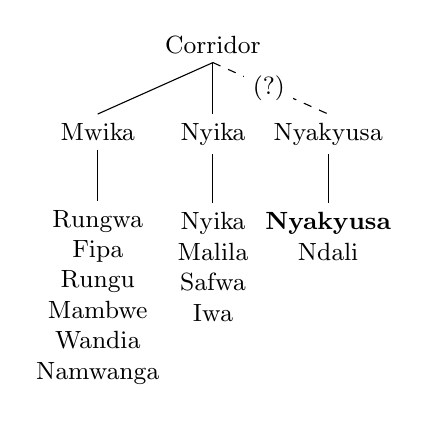
\begin{tikzpicture}[level distance=2.5em,
			sibling distance=8em,
			parent anchor=south,
			child anchor=north,
			anchor=north,
			align=center]
\small
\node(A){Corridor}
	child[sibling distance=4.5em]
			{node {Mwika} edge from parent[solid]
				child[sibling distance=4.5em]	
					%%M26 Iwa zweimal? Am Buch checken!		
					{node {Rungwa\\Fipa\\Rungu\\Mambwe\\Wandia\\Namwanga} edge from parent[solid]}
			}
	child[sibling distance=4.5em]
			{node {Nyika} edge from parent[solid]
				child[sibling distance=4.5em]
					{node {Nyika\\Malila\\Safwa\\Iwa} edge from parent[solid]}	
			}
	child[sibling distance=4.5em]
			{node (B){Nyakyusa} edge from parent[dashed]
				child[sibling distance=4.5em]
					{node {\textbf{Nyakyusa}\\Ndali} edge from parent[solid]}
			}	
;	
\path (A) -- coordinate[midway](AB) (B);
\node [anchor=center,fill=white] at (AB) {(?)};
\end{tikzpicture}
\caption{Nurse \& Phillipson's (\citeyear{NurseDPhillipsonG2003b}) classification of the Corridor languages}\label{ClassificationNursePhillipson2003}\il{Rungwa}\il{Fipa}\il{Rungu}\il{Mambwe}\il{Wandia}\il{Namwanga}\il{Nyika}\il{Malila}\il{Safwa}\il{Iwa}\il{Ndali}
\end{center}
\end{figure} 
Catherine Labroussi's (\citeyear{LabroussiC1998}, \citeyear{LabroussiC1999}) work is a valuable contribution to our understanding of the Corridor languages: apart from phonological traits and lexicostatistic calculations, it examines patterns of diffusion and also discusses social factors, mostly retrieved by archaeology and oral history. As for the classification of the Corridor languages, it fundamentally reflects Nurse's position concerning Nyakyusa.

Historian Christopher Ehret (\citeyear{EhretC1973}) proposed a Corridor-group (``Mambwe-Fi\-pa-Nyiha'')\il{Mambwe}\il{Fipa}\il{Nyika} which excludes Nyakyusa. What distinguishes his proposal is that he postulates that Corridor and Nyakyusa may belong to different branches of eastern Bantu. This position is revised in \citet[36f, 55]{EhretC2001}, where the Corridor languages are split into two major groups, Rungwe (Nyakyusa, Ndali,\il{Ndali} Safwa,\il{Safwa} Nyika,\il{Nyika} Wandia\il{Wandia}) and Mwika (Pimbwe,\il{Pimbwe} Fipa,\il{Fipa} Mambwe,\il{Mambwe} Namwanga\il{Namwanga}). Ehret qualifies this insofar as he admits that this synchronic grouping need not reflect linguistic genealogy.

Ehret's student Catherine Fourshey, however, has returned to Ehret's earlier views \citep{FoursheyC2002}. In an attempt to reconstruct the pre-colonial history of the Corridor based mainly on linguistic data, she proposes a genetic unit comprising the Corridor languages, the internal structure of the unit in essence reflecting Nurse's classification. Fourshey arrives at this assumption primarily on the basis of lexicostatistics supplemented and refined by an examination of the distribution of certain cultural lexemes. Unfortunately Fourshey did not have access to the linguistically more fine-grained analysis of \citet{LabroussiC1998}.

To conclude, it seems safe to assert at this point -- as stated more or less explicitly in \citet{NurseD1988}, \citet{LabroussiC1998}, \citet{NurseDPhillipsonG2003b} -- that the languages of the Corridor might best be understood not as a genetically uniform unit, but as forming an area of long-term linguistic convergence. In this context, Nyakyusa can be understood as the special case, being more strongly isolated from its geolinguistic environment. Although it shares a number of lexical and structural features with its neighbouring languages, especially \ili{Ngonde} and \ili{Ndali}/Sukwa,\il{Sukwa} it seems to have been rather resistant to external influences, and in the development and spreading of innovations it seems to have played the role of donor rather than that of recipient.

\largerpage[-2]
\subsection{Dialects and variety described}\label{InternalClassiffication}
\is{dialects|(}
The dialectal geography of the Corridor as a whole, as well as for the specific case of Nyakyusa, remains relatively unknown (\citealt[4, 25]{WalshMSwillaI2002}). However, a number of topolectal divisions can be stated. Some first observations concerning subgroups and varieties of Nyakyusa were made by \citet[61]{JohnstonH1977}, with subsequent refinements by \citet[2]{WilsonM1963}. The following notes are based on the latter, as well as on \citeauthor{WalshMSwillaI2002}'s (\citeyear{WalshMSwillaI2002}) comments upon it. These sources have been supplemented by consultation with a number of native speaker informants as well as by an unpublished survey by SIL International.\footnote{Kindly made available to the author by Helen Eaton.\ia{Eaton, Helen}} The following list gives the identifiable subgroups within Nyakyusa, together with their respective Guthrie codes according to \citet{MahoJ2009}:\footnote{It has to be kept in mind that ethnic or group identity and linguistic varieties need not overlap.}
\begin{compactitem}
\item Nyakyusa of the lake-shore plains. This variety is often referred to as \textit{MuNgonde} by speakers of northern varieties, although speakers from the area do not use this name themselves. It is considered clearly distinct from Malawian \ili{Ngonde} (\mbox{\textit{IkyaNgonde}}).
\item Central Nyakyusa, around Masoko. The Nyakyusa variety of this area, seat of chief Mwaipopo, is considered the variety with the highest prestige. In \citet{MahoJ2009} this variety is grouped with that of the lake-shore plains as \textit{Nyakyusa proper} (M31A).
\item Northern Nyakyusa (M31B), also called \textit{Kukwe} or \textit{Ngumba} (`innermost plateau').
\item Nyakyusa of the mountains (M31C), also referred to as \textit{Mwamba} (`Mountains'), \textit{Lugulu} (name of an aboriginal group) or \textit{Sokelo} (`East'), in the area around Mwakaleli.
\item Selya (M31E), at the foot of the Livingstone Mountains. Wilson distinguishes this from another eastern subgroup named Saku.
\end{compactitem}
The denominations for the various groups and varieties within Nyakyusa are used differently by speakers from different areas. As Monica Wilson states:
\begin{quote}AbaMwamba means by derivation `the hill people', but is generally used for `the people of the north'. The \ili{Ngonde} of Karonga call those on the plain around Mwaya BaMwamba, the men of Mwaya apply the name not to themselves, but to the people of Selya, while the people of Selya apply it to those in the hills to the north of them. \citep[2 FN2]{WilsonM1963}
\end{quote}
\largerpage[-2]
Two further varieties of unclear status might be added to the list above. \citet[9]{WilsonM1958} observed that the group of \ili{Penja} M302, as well speakers of the eastern variety of \ili{Nyika} M23, were being absorbed by the Nyakyusa. While the case of \ili{Penja} remains unsolved \citep[26]{WalshMSwillaI2002}, a recent sociolinguistic survey provides further indications of a language shift of the Eastern \ili{Nyika} people, suggesting an additional Nyakyusa topolect \citep{Lindforsetal2009}. 

Although diatopic variation within Nyakyusa exists and speakers readily identify the speech varieties of different regions, intercomprehension is not affected. Given the high number of speakers, Nyakyusa can be considered relatively uniform in comparison to many of the other, smaller Corridor languages (see \citealt[204]{LabroussiC1998}). Most speakers consulted stress that the main dividing line lies between the variety of the lake-shore plains (Kyela district) on the one side and the varieties of the more mountainous terrains on the other.

The focus of this study lies on the Selya and Mwamba/Lugulu varieties. The Germany-based language assistants are originaly from Ikama (Mwamba/Lugulu) and Itete (Selya). In Mbeya city, preliminary work was performed with speakers from Itete. The main part of the fieldwork (\sectref{DataCollection}) took place in the village of Lwangwa, which is said to be at the transition between the Mwamba/Lugulu and Selya varieties. The map in \figref{MapLwangwaIkamaItete} shows the position of the three villages.

\begin{figure}[hbt]
\begin{center}
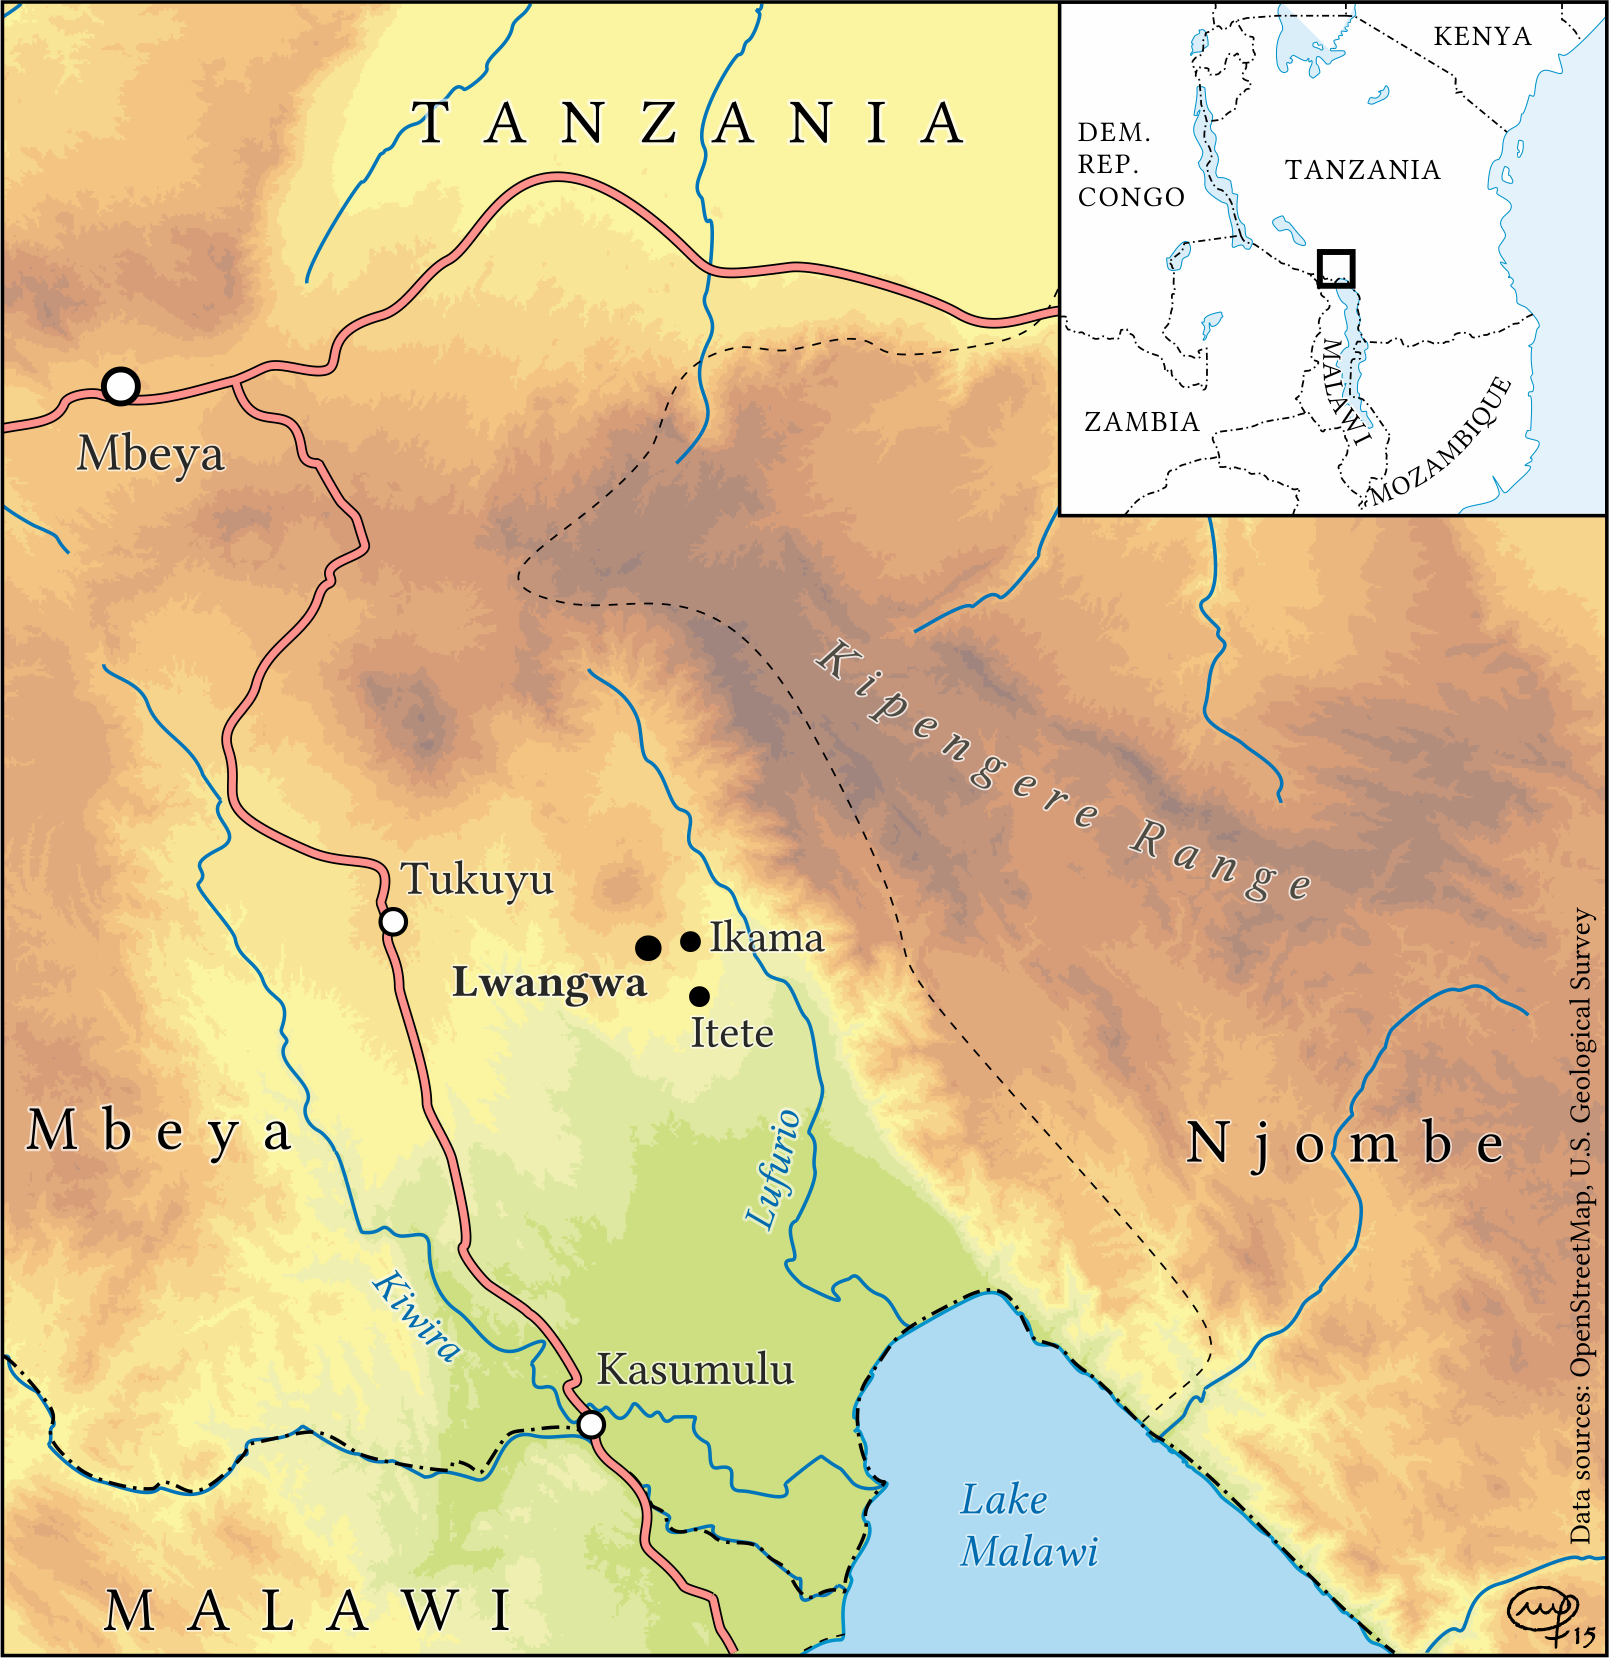
\includegraphics[width=0.75\textwidth]{figures/MapLwangwaIkamaItete.png}
\caption{Field base and origin of language assistants. Map courtesy of Monika Feinen}
\label{MapLwangwaIkamaItete}
\end{center}
\end{figure}

\label{Varietydescribed}
 \is{dialects|)}
\section{Data collection}\label{DataCollection}
The main data for this study was collected during three research trips to Tanzania. The first trip took place in November and December 2013, during which time research was carried out with speakers living in the city of Mbeya. On the second trip, in November and December of 2014, as well as on the third trip, from late September to early December of 2015, Lwangwa village in Busekelo district was chosen as the field base. Further intensive work, mainly guided elicitation, was carried out with two language assistants living in Germany between 2012 and 2016.

All language assistants that participated in this study are native speakers of Nyakyusa, fluent in Swahili and between 25 years and 78 years of age during the period of research. The expatriate speakers have been living in Germany since 2009 and 2005 respectively. Since that time they have returned periodically to the language area and continue to converse with family members on a regular basis in their native language. The contact language used in research has mainly been English, plus some Swahili (in Tanzania) and German (in Germany). 

The main practices of data collection were one-on-one elicitation and text collection, predominantly of folk narratives. Elicitation is here to be understood not as a mere production task, but in a broad and interactive sense, in line with \citet[2]{MousM2007}, who states that ``elicitation is guided conversation about language data''. See \citet[245--256]{CoverR2015} for a recent discussion of elicitation with a focus on semantic fieldwork.

The collection of lexical items, apart from basic approaches such as the elicitation of semantic fields and sound-substitution \citep[104--111]{CrowleyT2007}, was greatly aided by previous work on Nyakyusa, especially \citeauthor{FelbergK1996}'s (\citeyear{FelbergK1996}) dictionary. Although a great number of entries had to be checked for accuracy, it served as a valuable starting point for enlarging the lexical corpus. All lexical items were entered into a database using Fieldworks Language Explorer (FLEx) software. In the course of research this was supplemented and double-checked with usage in texts and spontaneous speech. FLEx software was also used for morphological segmentation and creating lexical cross-references. Given the problematic representation of Nyakyusa in several recent publications (see \sectref{ResearchHistory}), 
a great amount of time and scrutiny was dedicated to checking and re-checking all transcriptions.

With regard to the semantics of TMA, elicitation encompassed a variety of tasks. One of them was translation from the contact language, mostly together with a discourse context. Here \citeauthor{DahlOe1985}'s (\citeyear{DahlOe1985}; \citeyear{DahlOe2000a}) tense and aspect questionnaires served as valuable points of departure. In other cases, the compatibility of a given construction with specific adverbials or lexical items was checked through grammaticality judgements, or possible contexts of use for constructed sentences were narrowed down through dialogue with the language assistants. The more research advanced, the more elicitation on TMA became intertwined with the analysis of texts and naturally observed data. Specific utterances were checked for their applicability and/or meaning in other contexts, and examples were manipulated in a targeted way, again checking for acceptability, changes in meaning, and possible contexts of use.

The texts used in this study came from two main sources. First, oral monologues, mostly folk narratives plus a few e\isi{expository} texts, were recorded with single speakers and later transcribed by the researcher. The transcription was then checked and the texts were translated into English with the help of a language assistant. Apart from minor exceptions, these were not the recorded speakers themselves. Additionally, two retellings of the Pear Story \citep{ChafeW1980} were recorded and one oral rendering of a traditional narrative was made available by Knut Felberg.
Furthermore, a number of written texts were made available by SIL International's Mbeya office. These stem from literacy workshops and are mostly fictitious narratives but also include a few \isi{expository} and \isi{procedural} and one \isi{behavioural} text. Five of these came edited and with translations into English, the others were translated with the language assistants. One additional written expository text was provided by one of the main language assistants. All written texts were double-checked for pronunciation. The composition of the text corpus is given in \tabref{CompositionTextCorpus}. A few additional examples were taken from a current draft of a Bible translation by SIL International (kindly made available by Helen Eaton\ia{Eaton, Helen}),\footnote{Scripture quotations from The Authorized (King James) Version. Rights in the Authorized Version in the United Kingdom are vested in the Crown. Reproduced by permission of the Crown’s patentee, Cambridge University Press.} HIV prevention materials produced by the same organization and older text collections (\citealt{BergerP1933}; \citealt{BusseJ1942}; \citeyear{BusseJ1949}).


\begin{table}[ht]
\begin{center}
\begin{tabular}{lllll}

\lsptoprule

\footnotesize{Genre} & \footnotesize{Medium} & \footnotesize{Source} & \footnotesize{N\textsuperscript{o}\xspace of texts} & \footnotesize{Avg. N\textsuperscript{o}\xspace of words}\\
\midrule

Narrative & Oral & Own fieldwork & 15 & 324\\
Narrative & Oral & Knut Felberg & 1 & 856\\
Narrative & Written & SIL & 16 & 285\\
Retelling & Oral & Own fieldwork & 2 & 430\\
Exposition & Oral & Own fieldwork & 3 & 351\\
Exposition & Written & Own fieldwork & 1 & 95\\
Exposition & Written & SIL & 2 & 247\\
Behavioural & Written & SIL & 1 & 129\\
Procedural & Written & SIL & 1 & 205\\
\lspbottomrule
\end{tabular}
\caption{Composition of the text corpus}
\label{CompositionTextCorpus}
\end{center}
\end{table}

The focus on \is{narrative} discourse is due to a number of reasons. The first reason is the availability of texts and the comparatively easy segmentation of narrative texts, given the time limits imposed upon this study. The second reason is the need for an adequate description of the dedicated narrative markers (\sectref{NarrativeMarkers}). Third, though monological in their form, narratives often contain language of other communicative situations, for instance episodes in dialogue form or embedded expository or behavioural discourse. The use of certain grammatical devices, especially TMA, in everyday discourse constitutes an area that is open for further research.

Apart from elicitation and text collection, a great deal of everyday life in the field was carried out using Nyakyusa. This allowed for the observation of language use in a more natural environment and proved a fruitful source for contextualized examples, which served as jumping-off points for further elicitation. Lastly, \ili{Proto-Bantu} reconstructions stem from the Bantu lexical reconstructions\nobreakspace 3 database \citep{BLR3}.

Throughout this study, examples from elicitation sessions are marked with the abbreviation \lq\lq[ET]''. Textual data is marked with a short version of the text's name, often the title of the narrative, such as \lq\lq[Crocodile and Monkey]''. Examples from participant observation or conversation are marked as \lq\lq[overheard]''.
\section{Theoretical framework}\label{TheoreticalFramework}
\subsection{Overview}
For most parts of this grammar, no particular framework has been adopted. Instead, the description is based on well-known descriptive and typological concepts. In those parts dealing with phonological, morphological and syntactic aspects, the description is guided by structural considerations, whereas in the discussion of the meaning and use of TMA categories, functional considerations are in the foreground.

However, to gain a more profound understanding of the organization of \isi{tense} and aspect,\is{aspect!grammatical} the cognitive framework developed by \citet{BotneRKershnerT2008} has been adopted, although an attempt was made to give a broad and dense description so as to facilitate translation into other frameworks. Botne \& Kershner's framework will be outlined in \sectref{TenseAspect}--\ref{InherentTemporalStructure}.
 
Further, to approach the uses of TMA categories in Nyakyusa \isi{narrative} texts, the analytic tools developed by \citeauthor{LabovWWaletzkyJ1967} (\citeyear{LabovWWaletzkyJ1967} and subsequent works) were applied and augmented by a number of concepts stemming from the works of Fleischman (esp. \citeyear{FleischmanS1990}) and \citeauthor{LongacreR1990} (esp. \citeyear{LongacreR1990}), as well as some insights into activation status by Prince (\citeyear{PrinceEF1981}; \citeyear{PrinceEF1992}). These are described in \sectref{ToolsNarrativeAnalysis}. Lastly, while the approaches mentioned so far are synchronically oriented, in various cases it was found that applying a diachronic perspective helped the understanding of the present-day situation. Therefore, findings from \isi{grammaticalization} theory (e.g. \citealt{HeineBClaudiUHuennemeyerF1991}; \citealt{BybeePerkinsPaglucia1994}) were included, particularly with regard to identifying the sources of a given construction, delimiting newer and older readings and disentangling the interplay between the various constructions available within an area of grammar.
\subsection{Tense and grammatical aspect}\label{TenseAspect}
\subsubsection{Tense}\label{Tense}
\is{tense|(}
Tense is a deictic category that localizes a described state-of-affairs in time (see \citealt{ComrieB1985} among others). According to the most commonly expressed view, the linguistic construal of time is best described in terms of an abstract time line. Thus \citet[2]{ComrieB1985}, in his reference work on tense, declares that \lq\lq such a diagrammatic representation of time is adequate for an account of tense in human language.” \figref{FigureLinearConceptionOfTime} illustrates this conception. Throughout this study, in the illustration of temporal relations, S stands for \lq time of speech’.

\begin{figure}[h]
\begin{center}
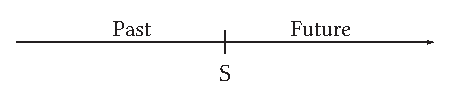
\includegraphics{figures/GrafikLinearTime.eps}
\caption{Linear conception of time}
\label{FigureLinearConceptionOfTime}
\end{center}
\end{figure}

Bantu languages are well known for their complex TMA systems which include various degrees of remoteness in time, especially in the past (\citealt[185]{DahlOe1985}; \citealt[21f]{NurseD2008}). Following the common conception of tense, these are usually described in terms of distance on a mono-dimensional timeline, as illustrated in \figref{FigureRemoteness}. The subscript digits indicate the degree of remoteness.

\begin{figure}[h]
\begin{center}
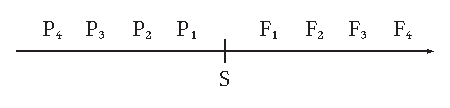
\includegraphics{figures/GrafikRemoteness.eps}
\caption{Remoteness distinctions in a linear conception of time}
\label{FigureRemoteness}
\end{center}
\end{figure}

Such a representation, however, fails in many cases to explain patterns of morphological marking, as well as the systematic employment of these constructions. For example, the Malawian Bantu language \ili{Sukwa} M301, as discussed by \citet[93f]{KershnerT2002}, possesses four non-imperfective paradigms with past time reference. At first glance, their meanings seem to represent a progression from immediate past to to remote past. \figref{FigureSukwaPasts} illustrates these paradigms together with their morphological composition on the traditional timeline.

\begin{figure}[hbt]
\begin{center}
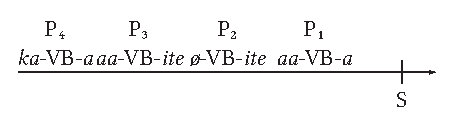
\includegraphics{figures/GrafikPastsSukwa.eps}
\caption{Sukwa paradigms with past reference. Adapted from \citet[94]{KershnerT2002}}
\label{FigureSukwaPasts}
\end{center}
\end{figure}

The linear approach to tense fails to give a motivated explanation for the morphological composition of these constructions, e.g., why there is a zero-prefix in past\textsubscript{2}, whereas past\textsubscript{1} and past\textsubscript{3} have \textit{aa}-, or why past\textsubscript{3} combines the prefix of past\textsubscript{1} with the suffix of past\textsubscript{2}. Further, it does not allow us to adequately describe their patterns of employment, which are described at length by \citet{KershnerT2002}.

To address such cases, \citet{BotneRKershnerT2008} develop a cognitive model of tense and aspect, which is based on the tenet that there are two basic conceptualizations of time. One conceptualization has Ego, the conceptualizer, moving along a stationary timeline (\textsc{time is a path}); see \citet[84f]{EvansVGreenM2006} on the concept of Ego. In the other, time itself is construed as moving (\textsc{time is a stream}), which allows for two perspectives. Either the metaphorical stream of time moves Ego along, passing eventualities as they take place, or time floats eventualities past a stationary Ego. \figref{FigurePerspectivesOnTime} depicts the two basic construals.

\begin{figure}[h]
\begin{center}
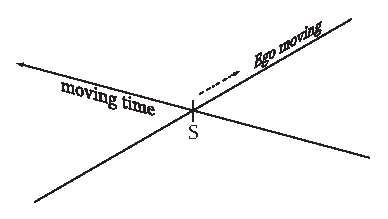
\includegraphics{figures/GrafikPerspectivesTime.eps}
\caption{Two perspectives on time}
\label{FigurePerspectivesOnTime}
\end{center}
\end{figure}

These two distinct conceptualizations of time are not mutually exclusive. A language may rather encode different aspects of both in different verbal paradigms. Botne \& Kershner go on to decompose \citeauthor{ReichenbachH1947}'s (\citeyear{ReichenbachH1947}) concept of reference time into two separate concepts: reference frame (\lq\lq temporal domain'' in Botne \& Kershner's terms) and reference anchor. The first is said to be \lq\lq comparable, but not identical'' \citep[152]{BotneRKershnerT2008} to \citeauthor{KleinW1994}'s (\citeyear{KleinW1994}) concept of topic time. Tense is then understood as the relationship between time of speech as the deictic locus and a reference frame. When the time span of the reference frame includes the deictic locus, this ``denot[es] a primary, prevailing experiential past and future perspective'' \citep[153]{BotneRKershnerT2008}. In cases where the deictic locus is not included in the time span of the reference frame (domain), they speak of a dissociated past or future. Exclusion corresponds to the conceptualization of \textsc{time} is a \textsc{path}.

The split between reference frame and reference anchor allows Botne \& Kershner to further account for temporal relations within a reference frame, which correspond to the conceptualizatioan of \textsc{time} is a \textsc{stream}. 

\figref{FigureConstrualsOfPast} illustrates these two types of temporal relationships, with the reference frames (domains) as rectangular plains. \figref{PastDDomain} depicts a past tense, such as the \ili{English} simple past. With the reference frame excluding the time of speech, the conceptualizer is instructed to move to a different cognitive domain, where the eventuality takes place. \figref{PastPDomain} illustrates an associated past (\lq\lq tenor'' in Botne \& Kershner's terminology), which situates an eventuality prior to the time of speech but within the same reference frame.

\begin{figure}[h]
\begin{center}
\caption{Dissociative and associative pasts}
\label{FigureConstrualsOfPast}
\begin{subfigure}[h]{0.45\textwidth}
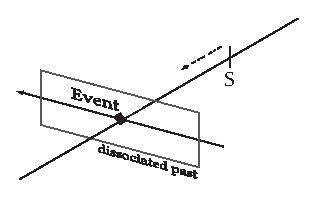
\includegraphics{figures/GrafikPastDDomainNew.eps}
\subcaption{Dissociative past}
\label{PastDDomain}
\end{subfigure}
\begin{subfigure}[h]{0.45\textwidth}
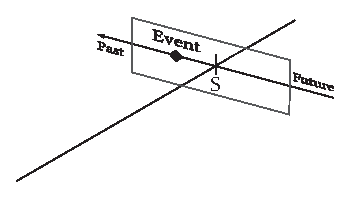
\includegraphics{figures/GrafikPastPDomainNew.eps}
\subcaption{Associative past}
\label{PastPDomain}
\end{subfigure}
\end{center}
\end{figure}
\largerpage
In the case of \ili{Sukwa} addressed above, constructions with past time reference can now be described on a compositional basis \citep{KershnerT2002}. The suffix \mbox{-\textit{ite}} denotes \textit{completive aspect}.\footnote{See \sectref{Aspect}, \ref{PerfectivityCompletion} on grammatical aspect\is{aspect!grammatical} and the notion of \isi{completion} respectively.} The prefix \textit{aa}- situates the described state-of-affairs in a preceding time unit within the same reference frame. In out-of-the-blue utterances this is understood as being shortly before the time of speech, but depending on the discursive environment, it can also refer to units such as the preceding day, month, season, etc.
The sense of heightened remoteness of the configuration \mbox{\textit{aa}-}\textsc{vb}\mbox{-\textit{ite}} then derives from viewing an event as already completed within a preceding time unit. Lastly, \textit{ka}- is a true tense in that it situates the state-of-affairs in a past reference frame. \figref{FigureSukwaTenorTense} illustrates the pasts of Sukwa.\il{Sukwa} See \citet{BotneRKershnerT2008} for a discussion of a number of such cases across Bantu.

\begin{figure}[hbt]
\begin{center}
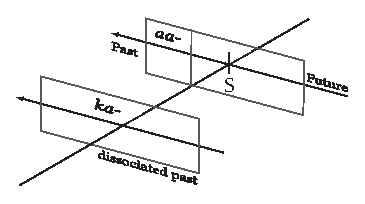
\includegraphics{figures/GrafikSukwaTenorTenseNew.eps}
\caption{Organization of the past in Sukwa. Adapted from \citet[113]{KershnerT2002}.}
\label{FigureSukwaTenorTense}
\end{center}
\end{figure}

Apart from Botne \& Kershner's own work (among others \citealt{BotneR2003b}; \citeyear{BotneR2006}; \citeyear{BotneR2008}; \citealt{BotneRKershnerT2000}; \citeyear{BotneRKershnerT2008}; \citealt{KershnerT2002}) their framework has proven fruitful in \citeauthor{SeidelF2008}'s (\citeyear{SeidelF2008}) grammar of \ili{Yeyi} R41, \citeauthor{CraneTM2011}'s (\citeyear{CraneTM2011}) treatise of tense and aspect in \ili{Totela} K41 as well as \citeauthor{DomSBostoenK2015}'s (\citeyear{DomSBostoenK2015}) work on the \ili{Kikongo} cluster of Bantu languages. As will be seen in Chapters \ref{TenseAspectConstructions}--\ref{Futurates}, the core assumption of two linguistic perspectives on time will also guide our understanding of the organization of the Nyakyusa tense and aspect system.
\is{tense|)}

 
\subsubsection{Grammatical aspect}\label{Aspect}
\is{aspect!grammatical|(}
While tense, as defined in \sectref{Tense}, is a deictic category, aspect is not. According to the most common and widely agreed-upon definition, ``aspects are different ways of viewing the internal temporal constituency of a situation'' \mbox{\citep[3]{ComrieB1976}.}

\newpage 
As has been pointed out variously in the theoretical literature on aspectuality, it is essential to distinguish aspect as a grammatical device from the aspectual potential encoded in the lexical verb or verb phrase. \citet{SasseHJ2002} speaks of \lq\lq bidimensional approaches'' to aspectuality. Within these bidimensional approaches, a prominent position is taken by those approaches which \citet{SasseHJ2002}, adopting a term first introduced by \citet{BickelB1997}, calls \lq\lq radical selection theories''. In these theories, aspect as a morphosyntactic device and the lexical dimension of aspect are understood as standing in a strict correspondence relationship: grammatical aspect serves as a phase-selector that selects matching temporal phases from the lexical dimension (the concept of phase will be developed in \sectref{InherentTemporalStructure}). As Sasse points out, other prominent bi-dimensional approaches to aspectuality, such as the one put forward by \citet{SmithC1997} are conceptually closely related to radical selection theories or might even constitute only a notional variant of them.

The need to distinguish two dimensions of aspectuality also holds for an adequate description of Nyakyusa. As will become clear in Chapters \ref{AspectualClassification}--\ref{Futurates}, grammatical aspect in Nyakyusa is sensitive to the aspectual potential in the lexical (and verb phrase) dimension and hence the choice of an inflectional paradigm greatly depends upon the latter. A central distinction here is that which falls between inchoative and non-inchoative verbs; see \sectref{AristotelianAspect}. In compliance with the tenets of radical selection theories, Botne \& Kershner define grammatical aspect as follows:

\begin{quote}
[Grammatical, BP] [a]spect denotes the particular temporal view of time in the narrated event. More precisely, a specific aspect denotes a particular temporal phase of the narrated event as the focal frame for viewing the event. This focal frame depicts the status of the event in relation to the vantage point determined by Ego, by default typically the moment of speaking. \citep[171]{BotneRKershnerT2008}
\end{quote}

It is not entirely clear how far the idea of a temporal phase as the ``focal frame'' serves our understanding of grammatical aspect in Nyakyusa. Rather, it seems, especially in the case of perfective aspect (\sectref{PerfectivityCompletion}), that Ego's vantage point may be construed in relation to a particular phase without necessarily being contained in the eventuality itself. Throughout this study, grammatical aspect will therefore be understood in a slightly simplified version of Botne \& Kershner's definition as denoting a particular temporal view of an eventuality by relating Ego's vantage point to a particular temporal phase of it.

As can be gathered from the preceding discussion, Botne \& Kershner's approach to tense and grammatical aspect is a compositional one. Concerning Nyakyusa, this has proven especially fruitful for the analysis of the past tense paradigms (see Chapter \ref{TenseAspectConstructions}), the function of the future enclitic \textit{aa}= (\sectref{ProcliticAa}) and the analysis of the present perfective (\sectref{PresentPerfective}) vis-à-vis the past perfective (\sectref{PastPerfective}). In a few other cases, such as the narrative tense (\sectref{NarrativeTense}) and the modal future (\sectref{ModalFuture}), the meanings and uses of the paradigms in question can, however, only be taken as a function of the entire construction. This situation can, in turn, be explained by taking into account the diachronic axis.
\is{aspect!grammatical|)}
\subsection{Inherent temporal structure of the verb}\label{InherentTemporalStructure}
Grammatical aspect,\is{aspect!grammatical} as defined in the previous subsection, relates Ego's vantage point to a particular temporal \isi{phase} of an eventuality. The key to the interpretation of any particular verbal expression in Nyakyusa is thus the interaction between grammatical aspect\is{aspect!grammatical} and the temporal structure inherently encoded in the verb. In spite of its central role, this facet of grammar hardly receives any attention in descriptive work on Bantu languages. It is common in Bantu studies, however, to recognize that a number of verbs tend to show a particular behaviour, appearing mainly in certain inflectional paradigms and encoding a state. This class of verbs is commonly labeled \lq\lq inchoative verbs'' (e.g. \citealt[55–60]{ColeD1955});\is{inchoative verbs} this class of verbs will be dealt with in more detail below. A brief theoretical digression will lay out the concepts and analytical tools central to understanding the interaction between the lexical and the inflectional dimension in Nyakyusa.
\subsubsection{Aristotelian aspect (\lq lexical aspect')}\label{AristotelianAspect}
\is{aspect!Aristotelian|(}Aristotelian aspect, also named \lq lexical aspect' or \lq verb aspect' by some scholars, refers to the obligatory classification of the aspectual potential encoded in the lexical (and phrasal) dimension in terms of abstract temporal phases. \citet{SasseHJ2002} speaks of \lq aspect\textsubscript{2}'. The present study follows Binnick's terminology, as \iai{Aristotle} is generally credited with discovering these distinctions \citep[171f]{BinnickR1991}.

The most familiar categorization of verbal expressions in the linguistic literature are the categories postulated by the philosopher \citet{VendlerZ1957} and developed to explain the behaviour of different verbal expressions in English.\il{English} Vendler\ia{Vendler, Zeno} distinguishes four types of expressions based on temporal criteria and their behaviour or compatibility in particular syntactic frames: states, activities, achievements and accomplishments. A major split between these categories is along the lines of telicity (delimitedness): achievements and accomplishments are understood as telic, whereas states and activities are understood as atelic. The latter two again differ in dynamicity, while accomplishments and achievements differ in regards to their duration (see below). Vendler's\ia{Vendler, Zeno} categories have been accepted by a great number of scholars as being valid for all natural languages, as they are supposed to be based on universals of logic and are therefore understood not to be subject to cross-linguistic variation (see e.g. \citealt[322]{TatevosovS2002}); for critical evaluations of this assumption see \citet{FilipH2011} and \citet{Bar-elL2015}. The broad acceptance of Vendler's\ia{Vendler, Zeno} categorization is not challenged by certain tweaks proposed by different scholars: for instance \citet{VerkuylH1972} and \citet{KennyA1969} conflate achievements and accomplishments, while \citet{SmithC1997} adds semelfactives as a further category. A number of tests to determine the category of different expressions have been developed in the literature, the most cited test being one for telicity, by checking for compatibility with adverbials of the type ``in X time'' and ``for X time''. For an overview of tests put forward by a number of scholars, see \citet[173–197]{BinnickR1991}.

For the study of Bantu languages Vendler's\ia{Vendler, Zeno} categories are hardly applicable. As \citeauthor{CraneTM2011} puts it:
\begin{quote}Rather than having a basic telic-atelic distinction, Bantu languages in general appear to divide verbs differently. This is due to a distinction between non-inchoative verbs (roughly corresponding to Vendler’s states, activities, and accomplishments) and inchoative verbs, which encompass many of Vendler’s\ia{Vendler, Zeno} achievements and other verbs. \citep[34]{CraneTM2011}\end{quote}

Crane hints at two closely related points of central importance. First, one essentially problematic category in Vendler's classification is that of achievement verbs. In a Vendlerian\ia{Vendler, Zeno} understanding, as echoed by \citet[195]{BinnickR1991}, ``an achievement is all culmination; although the achievement is possibly preceded by some activity […] the verb refers only to the achievement phase, not to the preceding activity''. \citet{PersohnB2017b}, by drawing on the Nyakyusa data presented in Chapter \ref{AspectualClassification} and incorporating data from \ili{Sukwa} \citep{KershnerT2002} and \ili{Ndali} \citep{BotneR2008}, shows that the morphosemantic behaviour of numerous verbal lexemes and verb phrases in these languages can only be explained by assuming the lexicalization of transitional patterns that consist of a state or process of origin, a change-of-state and a resultant state; similar assumptions have so far been mostly implicit in recent studies of aspectuality in Bantu languages. This leads to the second point: Crane picks up the notion of \textit{inchoative verbs},\is{inchoative verbs} which has come to be used as an umbrella term for those classes of verbal lexemes that encode a resultant state as part of their aspectual potential. As will become more explicit in Chapters \ref{AspectualClassification}--\ref{TenseAspectConstructions}, this notion of inchoativity plays a central role in the choice of grammatical aspect in Nyakyusa.

Within radical selection theories of aspectuality (\sectref{Aspect}), certain modifications of the Vendlerian\ia{Vendler, Zeno} categories have been stipulated. To give an example, Breu and Sasse (e.g. \citealt{BreuW1984}; \citealt{SasseHJ1991}) understand grammatical aspect\is{aspect!grammatical} as making reference to boundaries of situations, the basic assumption being that the lexical or verb phrase dimension can potentially encode one situation, a left boundary that represents the ingression into the situation and a right boundary, that is, the egression out of the situation. This yields five potential types of verbs. Other radical selection theories, such as \citet{BickelB1997} or \citeauthor{JohansonL1996} (\citeyear{JohansonL1996}; \citeyear{JohansonL2000}) offer comparable classifications; see \citet[48–52]{CroftW2012} for an overview. What these approaches share is the basic assumption that the lexical or verb phrase dimension may encode only one situation (or \lq middle phase'), which by definition excludes any lexicalizations of a transition from a state or process of origin into a resultant state; see \citet{PersohnB2017b} for more extensive discussion.

For the description of aspectuality in Nyakyusa the present study thus draws on a framework developed by Botne and Kershner (see \citealt{BotneR1983}; \citealt{KershnerT2002}; \citealt{BotneRKershnerT2008} among others; see also \sectref{TenseAspect}), which has its origin in Botne's study of aspectuality in Ruanda JD61 and has been extended by Kershner's study of Sukwa M301.\il{Sukwa} Botne and Kershner's categorization of verbs is based on \citet{FreedA1979}, a study of \ili{English} \isi{phasal verbs} (\lq aspectualizers') and their interaction with verbal semantics and the syntax of the verbal complement, in which Freed provides a formalization of Vendler's\ia{Vendler, Zeno} categories. In analogy with syllable phonology Freed\ia{Freed, Alice} proposes that the underlying temporal structure of verbs can be understood as a combination of three phases\is{phase} (\lq\lq segments'' in her terminology). The Onset\is{phase!Onset phase} constitutes a preliminary or preparatory phase, while the Nucleus\is{phase!Nucleus phase} corresponds to the characteristic act encoded in the verb. The Coda\is{phase!Coda phase} constitutes a culminative phase following the characteristic act. In doing so, Freed\ia{Freed, Alice} subscribes to Vendler's\ia{Vendler, Zeno} understanding of achievements as pure transitions. Botne and Kershner, in their works, adopt Freed's\ia{Freed, Alice} understanding of phases;\is{phase} their central modification is to allow for more combinations of phases.\is{phase} Thus achievement verbs, apart from a punctual Nucleus,\is{phase!Nucleus phase} may further encode an extended Onset\is{phase!Onset phase} (state of origin) and/or an extended Coda\is{phase!Coda phase} (resultant state), yielding four types of achievements. Likewise, accomplishments may either contain a punctual or extended Coda\is{phase!Coda phase} phase. In both cases, the presence or absence of an extended Coda phase\is{phase!Coda phase} is equivalent to the distinction between inchoative\is{inchoative verbs} and non-inchoative verbs. Activities, in Botne \& Kershner's understanding, comprise an extended Nucleus,\is{phase!Coda phase} whereas a state does not possess any internal structure. Throughout this study, in illustration of aspectual classes the three possible constituent phases\is{phase} will be abbreviated as O, N and C respectively. Note that the choice of Botne \& Kershner's model is to be understood as a useful descriptive tool; see \citet{PersohnB2017b} for a critical evaluation.   

What must be emphasized in this context is the essential need to distinguish between the ontology of a real world state-of-affairs on the one hand and the linguistic construction (lexicalization) on the other which need not be congruent (\citealt[77–100]{BotneR1981}; \citealt{BickelB1997}). Stated differently, cross-linguistic differences can arise when different phases\is{phase} of a situation are included in the lexical semantics of a verb. This is illustrated by \citet{BotneR2003b}, a case study on \lq to die' verbs, traditionally understood as a primary example of an achievement in Vendler's\ia{Vendler, Zeno} sense. Furthermore, the alleged polysemy of many inchoative verbs\is{inchoative verbs} in Bantu (\lq to become X'; \lq to be X') can thus be understood as a result of an inadequate meta-language translation, rather than an as inherent ambiguity (cf. \citealt[269, FN 249]{SeidelF2008}).
\subsubsection{Aktionsart}\label{Aktionsart}
\is{aktionsart|(}Having broached the issues of grammatical aspect\is{aspect!grammatical} and Aristotelian (lexical) aspect,\is{aspect!Aristotelian} a further analytical distinction is to be made between Aristotelian aspect and Aktionsart. While Aristotelian aspect classifies the phasal structure of the verb in a wider sense, Aktionsart is ``rather a classification of (expressions for) phases of situations and subsituations'' (\citealt[170]{BinnickR1991}), which is optional and best described in more specific terms such as inceptive or resumptive \citep[ibid]{BinnickR1991}. Formally, Aktionsart in Nyakyusa is expressed by verbal derivation (Chapter \ref{VerbalDerivation}) and \isi{phasal verbs} (Chapter \ref{AspectualClassification}).

To give an example, in the single-event reading of (\ref{exAktionsart}) the phasal verb\is{phasal verbs} \textit{leka} \lq cease, stop' refers to a cessation of the Nucleus phase of the lexical verb \textit{moga} \lq dance':

\begin{exe}
	\ex\label{exAktionsart}
	 \gll a-lek-ile ʊ-kʊ-mog-a\\
	1-cease-\textsc{pfv} \textsc{aug}-15(\textsc{inf})-dance-\textsc{fv}\\
	\glt \lq S/he has stopped dancing.'
\end{exe}
\is{aktionsart|)}
\subsection{Tense and grammatical aspect in discourse}\label{TenseAspectDiscourse}
\subsubsection{Remarks on textual analysis and grammaticography}
In the following description of tense and aspect categories, apart from their use in a sentence-level frame, an attempt is made to further include their use in discourse. A number of factors speak in favour of this approach. The \lq traditional' perspective on tense and aspect is most clearly expressed by Comrie:
\begin{quote}{[T]he investigation of the use of a grammatical category in discourse should not be confused with the meaning of that category; instead, the discourse function should ultimately be accounted for in terms of the interaction of meaning and context. \citep[29]{ComrieB1985}}\end{quote}

Among the well-known feature of Bantu languages, however, are constructions whose main function lies in the structuring of narrative discourse \citep[24]{NurseD2008}, typically labelled \textit{narrative tense} and/or \textit{consecutive tense}; see Chapter \ref{NarrativeMarkers} for such constructions in Nyakyusa.\is{narrative markers} Thus Comrie's perspective seems problematic with regard to descriptive adequacy. A similar argument is put forward by \citet{GueldemannT1996} in his discussion of Doke's grammar of \ili{Lamba} M54 (translated from the original German, BP):
\begin{quote}{In the otherwise extensive and precise grammatical analysis by Doke one hardly encounters useful indications concerning the construction's functional classification […] The author only describes the verbal paradigm with\-in the limits of sentence semantics […] Within such an approach the result of the analysis can only produce a relatively vague term such as tempus historicum, which semantically speaking seems the more vacuous as the paradigms characterized by it are not the only ones that can denote historical events. \citep[208]{GueldemannT1996}}\end{quote}

Furthermore, as \citet[77ff]{LevinsonS1983} notes, in most languages there is no one-to-one correspondence between temporal reference, in the physical sense, and linguistic categories. It is a common feature of natural languages to employ the latter for a broader variety of meanings. Assuming these notions surface especially in discourse contexts, an analysis limiting itself to the sentence-level misses many defining characteristics.

The opposite pole to a position such as Comrie's is prominently represented by \citet{WeinreichH1964} and \citet{HopperP1982}, who consider temporal and aspectual categories to be of discourse origin and sentence-level meanings to be but mere correlates of discourse functions. Hopper says:
\begin{quote} {[M]orphological and local-syntactic accounts of aspect are either incomplete, or, to the extent that they are valid, essentially show the sentence-level correlates of discourse structures […][O]ur understanding of aspect should be rooted in the last resort in discourse. \citep[16]{HopperP1982}}\end{quote}

An intermediate position is taken by Suzanne Fleischman, who considers discursive uses of \isi{tense} and grammatical aspect\is{aspect!grammatical} as ``motivated extensions that […] may ultimately contribute to a reshaping of the basic meanings'' \citep[23]{FleischmanS1990}. In other words, she sees a certain dialectic relationship between meaning and use, although with a primacy of meaning.

Further intermediary positions can be found in the field of cognitive linguistics, with approaches considered to be holistic. Mental space theory \citep{FauconnierG1994} deals with the construction of discursive worlds through the use of TMA markers among other features. To a certain extent Botne \& Kershner's principle of inclusion and exclusion (\sectref{Tense}) can also be understood as holistic, although no direct reference to discourse is made. What both approaches and further cognitive frameworks have in common is that, in their understanding, temporal and aspectual interpretations of these inflectional categories represent just the special case of a more general notion of cognitive distance and accessibility.

Independently of which one of these intermediary positions is taken, this short excursion has shown that it is necessary to include sentence-level as well as discursive data, whether they permit us to draw conclusions as to the \lq\lq basic'' meanings of the categories in question, which might be in the process of being reshaped by discursive use, which again is culture- and language-specific, or because sentence-level semantics and discourse uses are understood as two sides of one abstract conceptualization.
\subsubsection{Tools and concepts of narrative analysis}\label{ToolsNarrativeAnalysis} \is{narrative|(}
The key concepts used in this study to approach the use of tense and grammatical aspect in discourse stem from \citeauthor{LabovWWaletzkyJ1967} (\citeyear{LabovWWaletzkyJ1967} and subsequent works). These authors propose a classification of independent clauses within narratives, based on whether and to what degree they can be displaced without changing the temporal and sequential interpretation:
\begin{compactitem}
\item \textit{Narrative clauses}\is{clause types (Labov \& Waletzky)!narrative clause} cannot be displaced without changing the inferred sequence of eventualities.
\item \textit{Restricted clauses}\is{clause types (Labov \& Waletzky)!restricted clause} can be displaced throughout a determined part of a narrative.
\item \textit{Co-ordinate clauses}\is{clause types (Labov \& Waletzky)!co-ordinate clause} can be interchanged only with each other.
\item \textit{Free clauses}\is{clause types (Labov \& Waletzky)!free clause} can range throughout the whole narrative.
\end{compactitem}

By moving each clause to the beginning of its respective displacement set and coalescing coordinate clauses into a single unit, the ``primary sequence'' of events is obtained. Labov \& Waletzky further put forward a structural outline of a typical narrative text (\tabref{tableNarrativeStructureLW1967}).

A minimal narrative, according to \citet{LabovWWaletzkyJ1967}, consists of a sequence of clauses of which at least two are temporarily ordered. Thus a minimal narrative may consist of only the complicating action,\is{section!complicating action} although Labov \& Waletzky emphasize that such a narrative would be pointless.
As \citet[136]{FleischmanS1990} observes, there is a close relationship between narrative structure and TMA categories. The abstract\is{section!abstract} and coda\is{section!coda} relate to the now of the speaker, thus one can expect the corresponding verbal categories to be used, whereas the orientation section,\is{section!orientation} the complicating action\is{section!complicating action} and the resolution\is{section!resolution} relate to the story-now and thus demand the use of different categories.

\begin{table}[H] % [H] sorgt dafür, dass genau hier und nicht verrutscht
	\centering
	
\begin{tabularx}{\textwidth}{lX}
\lsptoprule 
\footnotesize{Abstract}\is{section!abstract} & A short summary that primarily serves to license the speaker to take the conversational turn. \\  
\footnotesize{Orientation}\is{section!orientation} & Formally defined as those free clauses preceding the first narrative clause. Its function is to ``orient the listener in respect to person, place, time and behavioural situation“ \citep[32]{LabovWWaletzkyJ1967}. \\ 
\footnotesize{Complicating action}\is{section!complicating action} & The core of the text. \\ 
\footnotesize{Evaluation}\is{section!evaluation} & The point of the narrative, defined semantically through evaluation of eventualities, allocation of blame, etc. The evaluation can coincide with other structural parts of the narrative. \\ 
\footnotesize{Resolution}\is{section!resolution} & Formally defined as the part of the narrative following or coinciding with the evaluation. In \citet[414]{LabovW1997} the definition is refined to ``the set of complicating actions that follow the most reportable event.''\\
\footnotesize{Coda}\is{section!coda} & ``[A] functional device for returning the verbal perspective to the present'' \citep[39]{LabovWWaletzkyJ1967}. The coda provides definite closure.\\
\lspbottomrule 
\end{tabularx} 
	\caption{Narrative structure according to \citet{LabovWWaletzkyJ1967}}
	\label{tableNarrativeStructureLW1967}
\end{table}

Labov \& Waletzky's analytic tools were originally designed for analysing ``oral versions of personal experience'' \citep[12]{LabovWWaletzkyJ1967}, which, according to the authors, exhibit the most simple and fundamental narrative structures. They were later successfully applied to more complex narrative texts, perhaps most prominently in the works of Suzanne Fleischman. Thus \citet{FleischmanS1990} is an extensive treatment of tense and grammatical aspect in narrative discourse. Her analyses over a variety of languages, historical stages and genres is guided by the distinction of four separate but interdependent functional components on which tense and grammatical aspect operate:
\begin{compactitem}
\item The so-called \textit{referential component} encompasses truth-conditional relations and what Fleischman takes to be the basic functions of TMA categories. As the term \textit{referential} is often associated with so-called referential theories of meaning (e.g. \citealt{OgdenCKRichardsIA1923}), this component will be referred to as \textit{semantics} in the narrow sense throughout this study.
\item \textit{The textual component}\is{component of meaning!textual} deals with grounding (the construction of relative salience within the text), with marking textual boundaries and with controlling the flow of information.
\item \textit{The expressive component}\is{component of meaning!expressive} provides social and attitudinal meanings, including evaluations and points of view.
\item \textit{The metalinguistic component}\is{component of meaning!metalinguistic} characterizes the discourse as such, by signalling specific styles, genres, registers and types of discourse.
\end{compactitem}

The assumption of a textual component\is{component of meaning!textual} of meaning will prove fruitful in the analysis of the employment of the past tense categories in narrative discourse (\sectref{PastPerfectiveNarrative}), while the expressive component\is{component of meaning!expressive} plays a role for the narrative present (\sectref{NarrativePresent}) and the employment of tense in relative clauses (\sectref{PRSnonPSTRelativeClauses}).\is{subordinate clauses!relative clause} Lastly, a metalinguistic component\is{component of meaning!metalinguistic} must be assumed, at least for the dedicated narrative markers (Chapter \ref{NarrativeMarkers}).

From \citet{LongacreR1996} the concept of narrative peak has been adopted. Longacre puts forth a structural outline of narratives comparable to the one proposed by Labov \& Waletzky. Unlike the latter authors, however, he distinguishes between two tiers: a notional structure and a surface structure. Peak is then understood as the surface realization of the notional elements of climax (``everything comes to a head […] contradictions, […] all sorts of tangles until confrontation is inevitable''; \citealt[35]{LongacreR1996}) and/or denouement (``a crucial event happens which makes resolution possible''; \citealt[35]{LongacreR1996}). Considering the grammatical and pragmatic devices used, peak is characterized as ``a zone of turbulence in regard to the flow of the discourse in its preceding and following parts'' \citep[38]{LongacreR1996}. Common strategies of peak-marking include a shift in tense and grammatical aspect, rhetorical underlining such as repetitions and paraphrases, the concentration of participants as if on a crowded stage, over-specification of referents, or a shift in vantage point, to name just a few.

\is{information status|(}Lastly, in the analysis of tense usage in relative clauses\is{subordinate clauses!relative clause} (\sectref{PRSnonPSTRelativeClauses}), Prince's (\citeyear{PrinceEF1992}) classification of information status has proven helpful. Prince introduces two binary distinctions, depending on whether information is new or old to the hearer (hearer-new/hearer-old) and new or old to the discourse (discourse-new/discourse-old). In an older taxonomy \citep{PrinceEF1981}, discourse-new/hearer-new information is labelled \lq\lq brand new information''. As information that is new to the hearer is likewise new to the discourse, these distinctions yield three logical combinations: discourse-new/hearer-new, discourse-new/hearer-old, and discourse-old/hearer-old. As a separate category, Prince proposes inferable information: a discourse may contain information that is technically discourse-new/hearer-new but can be inferred from schemata, general beliefs or context. For Prince, information means referents in discourse. In the analysis of tense-use in relative clauses this study follows \citet{LevinsohnH2007} in applying the classification of activation status not only to referents, but to whole propositions, too. This combined approach to relative clauses has been adapted from \citet{KarelsJ2014}. \is{information status|)} \is{narrative|)}  
 \chapter{Grammatical sketch}
\section{Typological overview}
Nyakyusa classifies as a typical Narrow Bantu language, while also showing some unique characteristics. This section will provide a summary of these characteristics, giving examples of a number of commonly mentioned defining features (\citealt{MoehligW1981}; \citealt{NurseDPhillipsonG2003a}). It will then provide a short grammatical sketch that will serve as a point of departure for a more detailed description of the verb.

The phonology of Nyakyusa proves to be typical for Narrow Bantu in terms of its symmetrical inventory of seven vowel qualities\is{vowels!inventory} and its phonotactics, although it can be considered innovative with regard to the loss of \isi{tone} (\sectref{Stress}). Nyakyusa also shows a rather particular variation from typical Narrow Bantu vowel harmony\is{vowels!vowel height harmony} and related processes (\sectref{MorphophonologyOfVerbalExtension}).

Concerning morphology, Nyakyusa is a highly agglutinative language, with a productive system of verbal derivation.\is{derivation} As will be described in \sectref{Negations}, it features various verbal negations,\is{negative} the functional distribution of which is uncommon from a pan-Bantu perspective. Nyakyusa further has an elaborate system of tense,\is{tense} aspect\is{aspect!grammatical} and \isi{mood} categories. An outstanding feature of Nyakyusa in this regard are the great number of \isi{futurate} constructions (Chapter \ref{Futurates}) in comparison to past tense\is{tense!past} forms, and the existence of two different \isi{narrative markers} (Chapter \ref{NarrativeMarkers}). Bantu morphology, especially derivational\is{derivation} morphology, has been described as showing a strong tendency towards \isi{templatic} structures \citep{HymanL2002}. Nyakyusa shows some intriguing cases of \isi{templatic} requirements in the phonological realisation of certain affixes and affix combinations (see \sectref{ApplicativizedCausatives}, \ref{Imbrication}) that are noteworthy even within the broader Bantu context.

When it comes to syntax,\is{syntax} the Nyakyusa \lq\lq basic'' word order is SVO. The language has compound verbs, that is auxiliaries\is{auxiliary} taking an inflected verb as a complement (see \sectref{Persistive}, \ref{MinorConstructions}). The language further has a well developed system of \isi{noun classes} and both subject-\is{subject marker} and object-marking\is{object marker} on the verb.

\section{Basic phonology}\label{BasicPhonology}
\subsection{Vowels and syllables}\label{VowelsAndSyllales} 
\subsubsection{Syllable structure}
Syllables in Nyakyusa can have any of the following structures:
\begin{exe}
		\ex
		\begin{tabbing}
			NCGVx\=x\textit{ʊ.lʊ.te.\textbf{ngaa}.no}x\=\kill%unnsinnszeile für tabulatoren
			V \> \textit{\textbf{ɪ}.kɪ.ko.ta}\> `chair' \\
			VV \> \textit{\textbf{ii}.si.kʊ}\> `day' \\
			CV \> \textit{ʊ.n.jwe.\textbf{go}}\> `noise' \\
			CVV \> \textit{a.\textbf{kaa}.ja}\> `homestead' \\
			CGV \> \textit{ɪ.\textbf{kya}.lo}\> `field' \\
			N\> \textit{ʊ.\textbf{m}.pʊ.nga}\> `rice'\\
			NCV \> \textit{ʊ.mu.\textbf{ndʊ}}\> `person' \\
			NCVV \> \textit{ʊ.lʊ.te.\textbf{ngaa}.no}\> `peace' \\		
			NCGV \> \textit{ɪ.\textbf{ngwe}.go}\> `spear'
		\end{tabbing}
\end{exe}

The possible syllable structures are subject to several distributional constraints: Syllables featuring an initial NC-cluster are not permitted following a syllabic nasal and syllabic nasals do not occur in word-final position. V and VV only occur in the initial position of a word or clitic group. Word-final vowels as a general rule are short, although there are several exceptions: the negated copula (optional, see \sectref{Copulae}), some cases of the associative marker -\textit{a}, some interjections such as \textit{ee} `yes' and a number of ideophones.\is{ideophones}

\subsubsection{Vowel inventory}
 \is{vowels!inventory|(}
Nyakyusa has a system of seven phonemic vowel qualities, as has also been reconstructed for \ili{Proto-Bantu} \citep[147]{SchadebergT2003b}. Phonetically, the mid-vowels are realized as open-mid vowels [ɛ, ɔ]. All seven vowel qualities occur as short and long.  Following Bantuist conventions, long vowels are represented by a sequence of two identical vowels.\footnote{This stands in contrast to Ndali,\il{Ndali} which has a reduced inventory of five phonemic vowel qualities, maintaining the inherited length opposition (\citealt{LabroussiC1998}; \citealt{BotneR2008}), and Ngonde,\il{Ngonde} which has further lost the opposition in quantity (\citealt{LabroussiC1998}; \citealt{KishindoP1999}).} \figref{exVokalsystem} illustrates the vowel inventory.
%\begin{exe}[h]
%\ex\label{exVokalsystem}
\begin{figure}[h]
	\begin{center}
		\begin{vowel}[plain,triangle]%Vokaldreiecke
			\putvowel{a}{2\vowelhunit}{3\vowelvunit}
			\putvowel{i}{0pt}{0pt}
			\putvowel{ɪ}{0,67\vowelhunit}{1\vowelvunit}
			\putvowel{e}{1,34\vowelhunit}{2\vowelvunit}
			\putvowel{o}{2,67\vowelhunit}{2\vowelvunit}
			\putvowel{ʊ}{3,34\vowelhunit}{1\vowelvunit}
			\putvowel{u}{4\vowelhunit}{0pt}
		\end{vowel}
		\begin{vowel}[plain,triangle]
			\putvowel{aa}{2\vowelhunit}{3\vowelvunit}
			\putvowel{ii}{0pt}{0pt}
			\putvowel{ɪɪ}{0,67\vowelhunit}{1\vowelvunit}
			\putvowel{ee}{1,34\vowelhunit}{2\vowelvunit}
			\putvowel{oo}{2,67\vowelhunit}{2\vowelvunit}
			\putvowel{ʊʊ}{3,34\vowelhunit}{1\vowelvunit}
			\putvowel{uu}{4\vowelhunit}{0pt}
		\end{vowel}
	\end{center}
\caption{Nyakyusa vowel system}\label{exVokalsystem}
\end{figure}


\subsubsection{Vowel length}\label{VowelLength}  \is{vowels!length|(}
Nyakyusa has both short and long vowels. They can be lexically specified or can arise through morphophonemic processes such as contact between heteromorphemic vowels (\sectref{HiatusSolution}) or as a compensation for the deletion of word-internal non-syllabic nasals (see p.\nobreakspace\pageref{NasalDelition} in \sectref{NasalDelition}). It is these contexts in which vowel length is distinctive. The minimal pairs in (\ref{exMinimalpaareVokLängeLex}) exemplify the distinctive lexical function of vowel length, while those in (\ref{exMinimalpaareVokLängeGramm}) show that vowel length is grammatically distinctive.
\begin{exe}
	\ex \label{exMinimalpaareVokLängeLex}
	\begin{tabbing}
		\textit{ʊkʊmanya}x\=`err, make a mistake'x\=vs.x\=\textit{ʊkʊʊmanya}x\=\kill
		\textit{ʊkʊtima}\>`to rain'\>vs.\>\textit{ʊkʊtiima}\>`to herd'
		\\\textit{ʊkʊlɪla}\>`to cry'\>vs.\>\textit{ʊkʊlɪɪla}\>`to eat with/for/at'
		\\\textit{ʊkʊmeta}\>`cut (esp. hair)'\>vs.\>\textit{ʊkʊmeeta}\>`bleat, cry like a goat'
		\\\textit{ʊkʊsala}\>`choose; pick'\>vs.\>\textit{ʊkʊsaala}\>`be(come) happy'
		\\\textit{ʊkʊbola}\>`rot, go bad'\>vs.\>\textit{ʊkʊboola}\>`cut; slaughter'
		\\\textit{ʊkʊtʊla}\>`err, make a mistake'\>vs. \>\textit{ʊkʊtʊʊla}\>`take from the head'
		\\\textit{ʊkʊfula}\>`castrate'\>vs.\>\textit{ʊkʊfuula}\>`undress; open knots'		
	\end{tabbing}	
	\ex \label{exMinimalpaareVokLängeGramm}
	\begin{tabbing}
		\textit{ʊkʊmanya}x\=`err, make a mistake'x\=vs.x\=\textit{ʊkʊʊmanya}x\=\kill
		\textit{ajengile}\>`s/he has built'\>vs.\>\textit{aajengile}\>`s/he built'\\
		\textit{ʊkʊmanya}\>`to know'\>vs.\>\textit{ʊkʊʊmanya}\>`to know me' \\
		\textit{ʊkʊsala}\>`to choose; pick'\>vs.\>\textit{ʊkʊʊsala}\>`to choose me'
	\end{tabbing}	
\end{exe}
A number of Bantu languages, including some of the neighbouring Corridor languages, restrict the occurrence of long vowels. For instance, in \ili{Malila} M24, a long vowel cannot surpass the fourth mora reckoned from the word end \citep{KutschLojengaC2007}. Nyakyusa, however, does not know such a constraint as the following examples illustrate.
\begin{exe}
	\ex
	\begin{tabular}[t]{@{}>{\itshape}ll}
		\textit{j\textbf{aa}katala} & \lq (then) it (class 9) got angry'\\
		\textit{\textbf{aa}l\textbf{aa}l\textbf{ʊʊ}siisye} & `s/he asked'\\
		\textit{b\textbf{aa}lʊʊki} & `oranges'
	\end{tabular}
\end{exe}
Long vowels can further be the result of compensatory lengthening before prenasalized plosives (see \sectref{NC-Clusters}). Vowels following glides (\sectref{glides}) are also realized with a slightly increased duration. As vowel length in these two environments is predictable, it is not given in the orthographic representation.
Generally speaking, vowels in a syllable bearing primary stress tend to be realized with a longer phonetic duration, especially in the penultimate syllable of a phrase. Nevertheless, the phonemic length distinction is still discernible in stressed syllables.\footnote{The accoustic study by \citet{vanEssenOKaehler-MeyerE1969} notes the same for nouns produced in citation form, hence a phonological phrase. Such cases of phonetic penultimate lengthening have been reported for a number of Bantu languages; see \citet[313]{HymanL2013} and references therein.} The only exception to the regular lengthening before prenasalized plosives is in imperatives (\sectref{Imperative}).

The opposite of compensatory lengthening is triggered by syllabic nasals (see \sectref{SyllabicNasals}).\footnote{The same effect is triggered by the object marker of noun class 1; see p.\nobreakspace\pageref{OMNCL1syllabic} in \sectref{OMNCL1syllabic}.} Any vowel preceding a syllabic nasal surfaces as short. The examples in (\ref{exNCvsSyllabicNasal}) illustrate the opposition between prenasalized plosives and syllabic nasals. In the practical orthography employed throughout this work, syllabic nasals are marked <n̩, m̩> preceding <b, d, g>, thus differentiating them from the voiced prenasalized plosives. As a nasal preceding a voiceless plosive or another nasal is always syllabic in Nyakyusa  -- see \sectref{SyllabicNasals}, \ref{PrenasalizedPlosives} -- syllabicity is not overtly indicated in these cases. Examples in (\ref{exVowelShortening}) show that a short vowel is pronounced where the outcome of morphophonology would otherwise be a long or lengthened vowel.

\begin{exe}
	\ex
	\begin{xlist}
		\sn
		\label{exNCvsSyllabicNasal}
		\begin{tabbing}
			{[}a.ŋ̩.ga.ˈni.ɾɛ{]}x\=`s/he loves him/her'x\=vs.x\=\kill
			{[}a.ŋ̩.ga.ˈni.ɾɛ{]}\>`s/he loves him/her\>vs.\>{[}aː.{\ᵑ}ga.ˈni.ɾɛ{]} `s/he loves me'
		\end{tabbing}
	\end{xlist}
	\ex \label{exVowelShortening} 
	\begin{xlist}
		\ex Long vowel (triggered by \textsc{1sg} prefix) shortened:
		\begin{tabbing}
			{[tʷa.ŋ̩.kʰɔ.ˈma.ɰa]}x\=(\degree ba-a-mu-kom-aga)x\=\kill
			{[na.ŋ̩.kʰɔ.ˈma.ɰa]}\>(\degree n-a-mu-kom-aga)\>`I was beating him/her'
		\end{tabbing}
		\ex Long vowel (outcome of vowel coalescence) shortened:
		\begin{tabbing}
			{[tʷa.ŋ̩.kʰɔ.ˈma.ɰa]}x\=(\degree ba-a-mu-kom-aga)x\=\kill
			{[β̞a.ŋ̩.kʰɔ.ˈma.ɰa]}\>(\degree ba-a-mu-kom-aga)\>`they were beating him/her'
		\end{tabbing}
		\ex Vowel shortening overrides compensatory lengthening:
		\begin{tabbing}
			{[tʷa.ŋ̩.kʰɔ.ˈma.ɰa]}x\=(\degree ba-a-mu-kom-aga)x\=\kill
			{[tʷa.ŋ̩.kʰɔ.ˈma.ɰa]}\>(\degree tʊ-a-mu-kom-aga)\>`we were beating him/her'
		\end{tabbing}
	\end{xlist}
\end{exe}
\is{vowels!length|)}\is{vowels!inventory|)}

\subsubsection{Vowel coalescence and glide formation}\label{HiatusSolution}\is{vowels!hiatus solution|(}
When heteromorphemic vowels within a word are juxtaposed, vowel coalescence and glide formation take place. The regularities differ slightly to the left and to the right of the root. (\ref{exVowelContacti}--\ref{exVowelContactu}) illustrate the outcome to the left of the stem, using the combination of subject prefix and verb stem. In the case of /u/-initial stems, the examples are nouns.\footnote{No verb stems beginning with /u/ are attested and no prefix contains the mid-vowels /e, o/; see \sectref{PhonologicalStructureVerbalMorphemes}.} Note that the outcome of vowel contact is independent of syllable count.

\clearpage % necessary to keep following examples together
\begin{exe}
	\ex 
	\label{exVowelContacti}
	\begin{tabbing}
		u + ax\=$\rightarrow$x\=waxx\=\textit{ʊmuunyu}x\=(\degree ʊ-mu-unyu)x\=\kill%Unsinnszeile für Tabulatoren
		i + i\>$\rightarrow$\>ii\>\textit{siisile}\>(\degree si-is-ile)\>`they (class 10) have come'\\
		i + ɪ\>$\rightarrow$\>yɪ\>\textit{syɪmile}\>(\degree si-ɪm-ile)\>`they (class 10) have stopped'\\
		i + e\>$\rightarrow$\>ye\>\textit{syegile}\>(\degree si-eg-ile)\>`they (class 10) have taken'\\
		i + a\>$\rightarrow$\>ya\>\textit{syagile}\>(\degree si-ag-ile)\>`they (class 10) have found'\\
		i + o\>$\rightarrow$\>yo\>\textit{syogile}\>(\degree si-og-ile)\>`they (class 10) have bathed'\\
		i + ʊ \>$\rightarrow$\>yʊ\>\textit{syʊmile}\>(\degree si-ʊm-ile)\>`they (class 10) have dried'\\ 
		i + u\>$\rightarrow$\>yu\>\textit{ɪfyuga}\>(\degree ɪ-fi-uga)\>`hoofs'
	\end{tabbing}
	\ex
	\begin{tabbing}
		u + ax\=$\rightarrow$x\=waxx\=\textit{ʊmuunyu}x\=(\degree ʊ-mu-unyu)x\=\kill%Unsinnszeile für Tabulatoren
		ɪ + i\>$\rightarrow$\>ii\>\textit{liisile}\>(\degree lɪ-is-ile)\>`it (class 5) has come'\\
		%\>\>\>\textit{ɪkiisʊ}\>(\degree ɪ-kɪ-isʊ)\>`land; country'\\
		ɪ + ɪ\>$\rightarrow$\>yɪ\>\textit{lyɪmile}\>(\degree lɪ-ɪm-ile)\>`it (class 5) has stopped'\\
		%\>\>\>\textit{ɪkyɪnja}\>(\degree ɪ-kɪ-ɪnja)\>`year'\\
		ɪ + e\>$\rightarrow$\>ye\>\textit{lyegile}\>(\degree lɪ-eg-ile)\>`it (class 5) has taken'\\
		%\>\>\>\textit{ɪkyeni}\>(\degree ɪ-kɪ-eni)\>`forehead'\\
		ɪ + a\>$\rightarrow$\>ya\>\textit{lyagile}\>(\degree lɪ-ag-ile)\>`it (class 5) has found'\\
		%\>\>\>\textit{ɪkyalo}\>(\degree ɪ-kɪ-alo)\>`farm'\\
		ɪ + o\>$\rightarrow$\>yo\>\textit{lyogile}\>(\degree lɪ-og-ile)\>`it (class 5) has bathed'\\
		%\>\>\>\textit{ɪkyolo}\>(\degree ɪ-fy-ola)\>`pouch, bag'\\
		ɪ + ʊ\>$\rightarrow$\>yʊ\>\textit{lyʊmile}\>(\degree lɪ-ʊm-ile)\>`it (class 5) has dried'\\
		%\>\>\>\textit{ɪkyʊma}\>(\degree ɪ-kɪ-ʊma)\>`property; riches'\\
		ɪ + u \>$\rightarrow$\>yu\>\textit{ɪkyuga}\>(\degree ɪ-kɪ-uga)\>`hoof'
	\end{tabbing}
	\ex
	\begin{tabbing}
		u + ax\=$\rightarrow$x\=waxx\=\textit{ʊmuunyu}x\=(\degree ʊ-mu-unyu)x\=\kill%Unsinnszeile für Tabulatoren
		a + i\>$\rightarrow$\>ii\>\textit{biisile}\>(\degree ba-is-ile)\>`they have come'\\
		%\>\>\>\textit{amiino}\>(\degree a-ma-ino)\>`teeth'\\
		a + ɪ\>$\rightarrow$\>ɪɪ\>\textit{bɪɪmile}\>(\degree ba-ɪm-ile)\>`they have stopped'\\
		%\>\>\>\textit{amɪɪsi}\>(\degree a-ma-ɪsi)\>`water'\\
		a + e\>$\rightarrow$\>ee\>\textit{beegile}\>(\degree ba-eg-ile)\>`they have taken'\\
		%\>\>\>\textit{ameebe}\>(\degree a-ma-ebe)\>`crows'\\
		a + a\>$\rightarrow$\>aa\>\textit{baagile}\>(\degree ba-ag-ile)\>`they have found'\\
		%\>\>\>\textit{amaani}\>(\degree a-ma-ani)\>`leafs'\\
		a + o\>$\rightarrow$\>oo\>\textit{boogile}\>(\degree ba-og-ile)\>`they have bathed'\\
		%\>\>\>\textit{amoobe}\>(\degree a-ma-obe)\>`fingers, toes'\\  check if semantically OK
		a + ʊ\>$\rightarrow$\>ʊʊ\>\textit{bʊʊmile}\>(\degree ba-ʊm-ile)\>`they have dried'\\
		a + u\>$\rightarrow$\>uu\>\textit{amungu}\>(\degree a-ma-ungu)\>`mushrooms'
	\end{tabbing}
	\ex
	\begin{tabbing}
		u + ax\=$\rightarrow$x\=waxx\=\textit{ʊmuunyu}x\=(\degree ʊ-mu-unyu)x\=\kill%Unsinnszeile für Tabulatoren
		ʊ + i\>$\rightarrow$\>wi\>\textit{twisile}\>(\degree tʊ-is-ile)\>`we have come'\\
		%\>\>\>\textit{ʊlwiho}\>(\degree ʊ-lw-iho)\>`law; custom; culture'\\
		ʊ + ɪ\>$\rightarrow$\>wɪ\>\textit{twɪmile}\>(\degree tʊ-ɪm-ile)\>`we have stopped'\\
		%\>\>\>\textit{ʊlwɪsi}\>(\degree ʊ-lʊ-ɪsi)\>`river'\\
		ʊ + e\>$\rightarrow$\>we\>\textit{twegile}\>(\degree tʊ-eg-ile)\>`we have taken'\\
		%\>\>\>\textit{ʊlwelo}\>(\degree ʊ-lʊ-elo)\>`fishing net'\\
		ʊ + a\>$\rightarrow$\>wa\>\textit{twagile}\>(\degree tʊ-ag-ile)\>`we have found'\\
		%\>\>\>\textit{ʊlwalo}\>(\degree ʊ-lʊ-alo)\>`base, foundation'\\
		ʊ + o\>$\rightarrow$\>oo\>\textit{toogile}\>(\degree tʊ-og-ile)\>`we have bathed' \\
		ʊ + ʊ\>$\rightarrow$\>ʊʊ\>\textit{tʊʊmile}\>(\degree tʊ-ʊm-ile)\>`we have dried'\\
		%\>\>\>\textit{ʊlʊʊbo}\>(\degree ʊ-lʊ-ʊbo)\>`big knife, sword'\\
		ʊ + u\>$\rightarrow$\>uu\>\textit{ʊtungu}\>(\degree ʊ-tʊ-ungu) \> \lq little mushrooms' %check if OK
	\end{tabbing}
	\ex\label{exVowelContactu}\begin{tabbing}
		u + ax\=$\rightarrow$x\=waxx\=\textit{ʊmuunyu}x\=(\degree ʊ-mu-unyu)x\=\kill%Unsinnszeile für Tabulatoren
		u + i\>$\rightarrow$\>wi\>\textit{mwisile}\>(\degree mu-is-ile)\>`you (pl.) have come'\\
		%\>\>\>\textit{ʊmwifwa}\>(\degree ʊ-mu-ifwa)\>`thorn'\\
		u + ɪ\>$\rightarrow$\>wɪ\>\textit{mwɪmile}\>(\degree mu-ɪm-ile)\>`you (pl.) have stopped'\\
		%\>\>\>\textit{ʊmwɪmbi}\>(\degree ʊ-mu-ɪmbi)\>`singer'\\
		u + e\>$\rightarrow$\>we\>\textit{mwegile}\>(\degree mu-eg-ile)\>`you (pl.) have taken'\\
		%\>\>\>\textit{ʊmwesi}\>(\degree ʊ-mu-esi)\>`moon; month'\\
		u + a\>$\rightarrow$\>wa\>\textit{mwagile}\>(\degree mu-ag-ile)\>`you (pl.) have found'\\
		%\>\>\>\textit{ʊmwafi}\>(\degree ʊ-mw-afi)\>`medicine to make sb. vomit'\\
		u + o\>$\rightarrow$\>oo\>\textit{moogile}\>(\degree mu-og-ile)\>`you (pl.) have bathed' \\
		%\>\>\>\textit{ʊmooto}\>(\degree ʊ-mu-oto)\>`fire'\\
		u + ʊ\>$\rightarrow$\>ʊʊ\>\textit{mʊʊmile}\>(\degree mu-ʊm-ile)\>`you (pl.) have dried'\\
		%\>\>\>\textit{ʊmʊʊji}\>(\degree ʊ-mu-ʊji)\>`breath; air; steam'\\ 
		u + u\>$\rightarrow$\>uu\>\textit{ʊmuunyu}\>(\degree ʊ-mu-unyu)\>`salt'
	\end{tabbing}
\end{exe}

The table in (\ref{exVowelContactPrefixingTable}) summarizes the outcome of left-of-the-stem (prefixing) vowel contact.

%\begin{table}
%\centering
%\captionabove{Adjacent vowels (prefixing):}
\begin{exe}\ex\label{exVowelContactPrefixingTable}
	Adjacent vowels (left of the stem):\\
	\begin{tabular}{c|ccccccc}
		\lsptoprule 
		\diag{.1em}{.5cm}{\footnotesize{V1}}{\footnotesize{V2}} & i & ɪ & e & a & o & ʊ & u \\ 
		\cline{2-8}
		i & ii & yɪ & ye & ya & yo & yʊ & yu \\ 
		ɪ & ii & yɪ & ye & ya & yo & yʊ & yu \\ 
		%e & /  & /  & /  & /  & /  & /  & /  \\ 
		a & ii & ɪɪ & ee & aa & oo & ʊʊ & uu \\ 
		%o & /  & /  & /  & /  & /  & /  & / \\ 
		ʊ & wi & wɪ & we & wa & oo & ʊʊ & uu \\ 
		u & wi & wɪ & we & wa & oo & uu & uu \\ 
		\lspbottomrule
	\end{tabular}
\end{exe}
%\end{table}
\noindent Noun class 9 prefix \textit{jɪ}- is exceptional. Its vowel assimilates to any following vowel (one may alternatively analyse this as vowel deletion with subsequent compensatory lengthening). (\ref{exConcordNCL9beforeVowel}) illustrates this for the subject prefix.
\begin{exe}
	\ex \label{exConcordNCL9beforeVowel}
	\begin{tabbing}
		\textit{jʊʊmile}x\=(\degree jɪ-ʊm-ile)x\=\kill
		\textit{jiisile}\>(\degree jɪ-is-ile)\>`it (class 9) has come'\\
		\textit{jɪɪmile}\>(\degree jɪ-ɪm-ile)\>`it (class 9) has stopped'\\
		\textit{jeegile}\>(\degree jɪ-eg-ile)\>`it (class 9) has taken'\\
		\textit{jaagile}\>(\degree jɪ-ag-ile)\>`it (class 9) has found'\\
		\textit{joogile}\>(\degree jɪ-og-ile)\>`it (class 9) has bathed'\\
		\textit{jʊʊmile}\>(\degree jɪ-ʊm-ile)\>`it (class 9) has dried'
	\end{tabbing}
\end{exe}

Juxtaposition of heteromorphemic vowels to the right of the root (suffixation and infixation) occurs productively only in a limited number of cases, one of which is derivational suffixes attached to monosyllabic verbs. This yields slightly ideosyncratic results; see \sectref{VHHMonosyllabicVerbs}. The other two are the suffixing of inflectional affixes to monosyllabic verbs and a process of infixing referred to as \textit{imbrication} (\sectref{Imbrication}).\is{imbrication} Unlike with prefixes, the low vowel /a/ followed by a front vowel yields /ee/.
\begin{exe}
	\ex
	\begin{tabbing}
		xxxxx\=xxxx\=xxxxxx\=xxxxxxxxx\=xxxxxxxxxxxxxx\=xxxxxxx\kill
		i + i\>$\rightarrow$\>ii\>\textit{inamiike}\>(\degree inami<i>k-e)\>`bend (tr).\textsc{pfv}'\\
		ɪ + i\>$\rightarrow$\>ii\>\textit{pɪliike}\>(\degree pɪlɪ<i>k-e)\>`hear; feel.\textsc{pfv}'\\
		e + i\>$\rightarrow$\>ii\>\textit{kemiile}\>(\degree keme<i>l-e)\>`bark at.\textsc{pfv}'
	\end{tabbing}
	\ex\begin{tabbing}
		xxxxx\=xxxx\=xxxxxx\=xxxxxxxxx\=xxxxxxxxxxxxxx\=xxxxxxx\kill
		a + i\>$\rightarrow$\>ee\>\textit{peegwa}\>(\degree pa-igw-a)\>`be given'\\
		\>\>\>\textit{egeeme}\>(\degree ega<i>m-e)\>`lean.\textsc{pfv}'
		\\a + ɪ\>$\rightarrow$\>ee\>\textit{peela}\>(\degree pa-ɪl-a)\>`give away'
	\end{tabbing}
	\ex
	\begin{tabbing}
		xxxxx\=xxxx\=xxxxxx\=xxxxxxxxx\=xxxxxxxxxxxxxx\=xxxxxxx\kill
		o + e\>$\rightarrow$\>we\>\textit{bwene}\>(\degree bo<e>n-e)\>`see.\textsc{pfv}'\\
		o + i\>$\rightarrow$\>wi\>\textit{kosomwile}\>(\degree kosomo<i>l-e)\> \lq cough.\textsc{pfv}'\\
		ʊ + i\>$\rightarrow$\>wi\>\textit{alwike}\>(\degree alʊ<i>k-e)\>`stand up.\textsc{pfv}'\\
		u + i\>$\rightarrow$\>wi\>\textit{afwile}\>(\degree afu<i>l-e)\>`crawl.\textsc{pfv}'
	\end{tabbing}
\end{exe}
\is{vowels!hiatus solution|)}

\subsection{Consonants}
\is{consonants|(}
\subsubsection{Consonant inventory}
\tabref{TableConsonantInventory} shows the 16 phonemic consonants of Nyakyusa as they are spelt in this study. Where the phonetic value differs from the graphic representation the latter is given in angle brackets.
\begin{table}[H] % [H] sorgt dafür, dass genau hier und nicht verrutscht
	
	
	\begin{tabular}{|l|c|c|c|c|c|c|}
		\hline & 
		\footnotesize{Bilabial}&
		\footnotesize{Lab. dent}&
		\footnotesize{Alveolar}&
		\footnotesize{Palatal}&
		\footnotesize{Velar}&
		\footnotesize{Glottal}\\	
		%jeweils die, die sich berühren weg, d.h. bilabial c| lab. dent c| etc
		\hline Plosive &  				% Plosive
		p  &							% Bilabial
		&							% Labiodental
		t  &							% Alveolar
		ɟ <j> &					% Palatal
		k &							% Velar
		\\							% Glottal
		\hline Nasal & 					% Nasal
		m &							% Bilabial
		&							% Labiodental
		n &							% Alveolar
		ɲ <ny> &						% Palatal
		ŋ <ng'> &  					% Velar
		\\							% Glottal
		\hline Fricative & 				% Fricative
		& 							% Bilabial
		f &							% Labiodental
		s &							% Alveolar
		&							% Palatal
		&							% Velar
		h \\						% Glottal
		\hline Approx. &				% Approx.
		β̞ <b>   &     			% Bilabial
		&						% Labiodental
		&						% Alveolar
		&						% Palatal
		ɰ <g> &				% Velar
		\\						% Glottal
		\hline Lat. Appr. & 			% Lat. Approx
		&						% Bilabial
		&						% Labiodental
		l &			% Alveolar
		& 						% Palatal
		&						% Velar
		\\						% Glottal
		\hline Glide & 				% Glides
		&						% Bilabial
		&						% Labiodental
		&						% Alveolar
		(j) <y>  &				% Palatal
		(w) &					% Velar
		\\						% Glottal
		\hline
	\end{tabular}	
	\caption{Nyakyusa consonant inventory}
\label{TableConsonantInventory}	
\end{table}

The glottal fricative is very rare. In most cases it can be regularly traced back to loans from \ili{Kinga} and \ili{Kisi} \citep[218]{LabroussiC1998}. \citet{NurseD1979} even considers it to be so marginal as to make its phonemic status dubious. The velar nasal is frequent phonetically, but rare in its occurrence underlyingly. The approximants are realized as plosives when following a nasal and as approximants elsewhere. Lateral /l/ is optionally realized as [ɾ$\sim$ɹ] after a front vowel in unstressed syllables, unless it is followed by a glide. The palatal plosive is typically realized as an affricate [d͜ʒ] when following a nasal. Voiceless plosives tend to be aspirated. The fricative /f/ in native material can regularly be traced back to a diachronic or synchronic process of spirantization;\is{spirantization} see \citet{BoestonK2008} on Bantu spirantization. Morphophonemic processes can, however, obscure this relationship, detaching the fricative from the triggering vowel (see \sectref{ReciprocalAndCausative}, \ref{ApplicativizedCausatives}).\footnote{Note also the verb stem \textit{fifa} `hide (intr.)' (variant \textit{fisa}) < PB *\textit{píc}, a clear case of historical assimilation.} Nasals preceding another consonant are generally homorganic and will be written as <m> before a labial and as <n> elsewhere. Consonants in loans from Swahili that are not adapted to the phoneme inventory of Nyakyusa will be written with their respective phonetic symbols.

\subsubsection{Glides}\label{glides}
Glides can be synchronically or diachronically traced back to the desyllabification of a vowel,\is{vowels!hiatus solution} although the quality of the underlying vowel is not synchronically discernible in all cases. The palatalized alveolar nasal is clearly distinct from the palatal nasal. In monitored speech it is realized as [ni̯]. The palatalized alveolar nasal will be written as <ni> throughout this study in order to distinguish it from the palatal nasal /ɲ/, represented by the digraph <ny>.  Glides normally do not appear before rounded back vowels, although some lexicalized exceptions occur. Vowels following glides are slightly lengthened (\sectref{VowelLength}).

\subsubsection{Prenasalized plosives}\label{PrenasalizedPlosives}
Prenasalization in Nyakyusa is limited to plosives (see \tabref{tabPrenasalizedConsonants}).
\label{NC-Clusters}
\begin{table}[H] % [H] sorgt dafür, dass genau hier und nicht verrutscht
	\centering
	\begin{tabular}{cccc}
		\lsptoprule
		{\footnotesize{Bilabial}}&		% Bilabial
		{\footnotesize{Alveolar}} & 		% Alveolar
		{\footnotesize{Palatal}} & 		% Palatal
		{\footnotesize{Velar}} 	 \\		% Velar
		\midrule
		ᵐb <mb> & ⁿd <nd> & ⁿd͜ʒ <nj> & {\ᵑ}g <ng> \\
		\lspbottomrule
		
		%			\hline
	\end{tabular}	
	\caption{Prenasalized consonants}	
	\label{tabPrenasalizedConsonants} 
	%Fussnote bzgl. [y] statt [j]
\end{table}
Prenasalized plosives are always voiced and homorganic.\footnote{This voicing rule distinguishes Nyakyusa from the \ili{Ngonde} variety described by \citet[278]{LabroussiC1998}, although it does apply in the variety described by \citet{KishindoP1999}.} Voiceless plosives turn into their voiced counterparts when preceded by a non-syllabic nasal, and the approximants /β̞, l, ɰ/ into their plosive counterparts. (\ref{exnyclasses910}) shows that preceding vowels the prefix of noun class 9/10 surfaces as \textit{ny}- (note that any vowel preceding or following this prefix surfaces as long; see \sectref{NominalMorphology}) and (\ref{exNCclasses910}) illustrates how this prefix induces prenasalization.  (\ref{exNC1sg}) illustrates prenasalization with the subject prefix of the first person singular.\footnote{Before certain object prefixes, the \textsc{1sg} subject prefix turns into a syllabic nasal; see \sectref{SubjectConcordsParticipants}.}
\begin{exe}
	\ex \label{exnyclasses910}
	\begin{tabbing}
		xxxxxxxxx\=xxxxxxxxxxxx\=xxxxxxxxxxxxxx\=xxxxxxx\kill 
		\textit{ɪɪnyiifi}\>(\degree ɪ-ny-ifi)\>`chameleons'
		\\\textit{ɪɪnyɪmbo}\>(\degree ɪ-ny-ɪmbo)\>`songs'
		\\\textit{ɪɪnyendo}\>(\degree ɪ-ny-endo)\>`journeys'
		\\\textit{ɪɪnyaala}\>(\degree ɪ-ny-ala)\>`grindstones'
		\\\textit{ɪɪnyoobe}\>(\degree ɪ-ny-obe)\>`fingers'
		\\\textit{ɪɪnyʊʊbo}\>(\degree ɪ-ny-ʊbo)\>`big knives'
	\end{tabbing}
	              \newpage 
	\ex \label{exNCclasses910}
	\begin{tabbing}
		xxxxxxxxx\=xxxxxxxxxxxx\=xxxxxxxxxxxxxx\=xxxxxxx\kill 
		\textit{ɪmbepo}\>(\degree ɪ-ny-pepo)\>`cold; air(s); spirit(s)'
		\\\textit{ɪndʊmi}\>(\degree ɪ-ny-tʊmi)\>`message(s), news'
		\\\textit{ɪnjʊni}\>(\degree ɪ-ny-jʊni)\>`bird(s)'
		\\\textit{ɪnguuto}\>(\degree ɪ-ny-kuuto)\>`cry / cries'
		\\\textit{ɪmbatɪko}\>(\degree ɪ-ny-batɪko)\>`procedure(s)'
		\\\textit{ɪndagɪlo}\>(\degree ɪ-ny-lagɪlo)\>`law(s); commission(s)'
		\\\textit{ɪngolo}\>(\degree ɪ-ny-golo)\>`louse(s)'
	\end{tabbing}
	\ex\label{exNC1sg}
	\begin{tabbing}
		xxxxxxxxx\=xxxxxxxxxxxx\=xxxxxxxxx\=xxxxxxxxxxxxxx\=xxxxxxx\kill 
		\textit{mbinyile}\>(\degree n-piny-ile)\>`I have bound' 
		\\\textit{ndaagile}\>(\degree n-taag-ile)\>`I have thrown'
		\\\textit{njaatile}\>(\degree n-jaat-ile)\>`I have taken a walk' 
		\\\textit{ngeetile}\>(\degree n-keet-ile)\>`I have watched'
		\\\textit{mbalile}\>(\degree n-bal-ile)\>`I have counted'
		\\\textit{ndɪlile}\>(\degree n-lɪl-ile)\>`I have cried'
		\\\textit{ngelile}\>(\degree n-gel-ile)\>`I have tested'
	\end{tabbing}
\end{exe}

Prenasalized consonants are not considered phonemic for a number of reasons. First, when they occur across morpheme boundaries, as in the above examples, they can clearly be analysed as the result of a nasal segment followed by a plosive or approximant. Second, the nasals involved are also found as single phonemes and the voiced plosives are regular allophones of /β̞, l, ɰ/ in a post-nasal context, as can also be seen with the syllabic nasals (\sectref{SyllabicNasals}). Further, their stem-internal distribution is very limited, the majority of cases being the second consonant of the stem. Last, they are rarely found in affixes. All of this speaks in favour of assuming syllable structures of the type /NC\ldots / rather than an additional set of phonemes. Note that prenasalization triggers lengthening of a preceding vowel,\is{vowels!length} as discussed in \sectref{VowelLength}.

\subsubsection{Syllabic nasals}\label{SyllabicNasals}
In the great majority of cases, syllabic nasals are the result of a series of morphophonemic processes affecting noun class affixes. The most frequently applying of these processes is deletion of the underlying high back vowel of the prefixes of noun classes 1, 3, and 18 in most pre-consonantal environments and subsequent syllabification of the nasal segment. Other sources include the first person singular subject prefix in determined phonemic and morphological contexts (see \sectref{SubjectConcordsParticipants}).

Syllabic nasals hardly ever appear morpheme-internally. Exceptions include \textit{mma} [ˈm̩.ma] `no' and related forms such as \textit{somma} [sɔ.ˈm̩.ma] `don't!', as well as \textit{nnoono} [n̩.ˈnɔː.nɔ] `so much' and \textit{nsyɪsyɪ} [n̩.ˈsʸɪˑ.sʸɪ] `skunk' (pl. \textit{bansyɪsyɪ}). In contrast to prenasalized plosives, syllabic nasals do not trigger voicing. Thus, in the graphic representation, the syllabicity of nasals is ambiguous only in sequences involving a voiced plosive, and will be marked <m̩, n̩> in this context. Further, syllabic nasals induce shortening of preceding long or lengthened vowels (see \sectref{VowelLength}).\is{vowels!length} Phonetically they are realized with a longer duration than non-syllabic nasals. As with prenasalized plosives, syllabic nasals as a general rule are homorganic to the following segment, and approximant phonemes are hardened to plosives. A syllabic nasal preceding /h/ is realized as velar. 
\begin{exe}
	\ex\begin{tabular}[t]{lll}
		\textit{ʊm̩belo}&(\degree ʊ-mu-belo)&`wind'\\
		\textit{ʊn̩dʊme}&(\degree ʊ-mu-lʊme)&`husband'\\
		\textit{ʊn̩gʊnda}&(\degree ʊ-mu-gʊnda)&`field, farm'\\
		\textit{ʊnhɪɪji}&(\degree ʊ-mu-hɪɪj-i)&`thief'
	\end{tabular}
\end{exe}
\is{consonants|)}
\subsection{Suprasegmentals}\label{Stress} 
\is{stress|(}Nyakyusa is not a tonal language, unlike the majority of Bantu languages (\citealt{KisseberthCOddenD2003} among others). The loss of inherited tone in Nyakyusa has been noted even in early studies (e.g. \citealt{NurseD1979}; \citealt{GuthrieM1967}; \citealt{vanEssenOKaehler-MeyerE1969}). Instead, Nyakyusa features a regular penultimate accent. The lack of phonemic tone makes Nyakyusa quite different from its close relative \ili{Ndali} (see e.g. \citealt{NurseD1988}; \citealt{BotneR2008}), although this characteristic is apparently shared with \ili{Ngonde} (\citealt{KishindoP1999}; \citealt{LabroussiC1999})\is{tone}. Every word in Nyakyusa is assigned stress on the penultimate syllable. However, words are often grouped together as a prosodic unit, in which case the penultimate syllable of the rightmost word receives a more pronounced stress.\footnote{See \citet{BickmoreLClemensL2016} on \ili{Tooro} JE12 for a similar case.} Typical cases are nouns followed by a determiner:
\begin{exe}
	\ex
	\glll ʊˌmwan(a) ˈʊjʊ\\
	ʊ-mu-ana ʊ-jʊ\\
	\textsc{aug}-1-child \textsc{aug}-\textsc{prox.1}\\
	\glt `this child'
	\ex
	\glll iiˌgalɪ ˈlyangʊ\\
	ii-galɪ lɪ-angʊ\\
	5-car 5-\textsc{poss.1sg}\\
	\glt \lq my car'
\end{exe}

In the same fashion, a determiner introducing a relative clause (see \sectref{RelativeClausss}) forms a prosodic unit with the following verb:
\begin{exe}
	\ex \glll ʊn̩ˈdʊngʊ ˌʊgʊ gʊˈkwisa aˈtwale ɪɪˌheela \\
	ʊ-mu-lʊngʊ ʊ-gʊ gʊ-kʊ-is-a a-twal-e ɪɪ-heela\\
	\textsc{aug}-3-week \textsc{aug}-\textsc{prox.3} 3-\textsc{prs}-come-\textsc{fv} 1-carry-\textsc{subj} \textsc{aug}-money(9)\\
	\sn \glll ˈjangʊ\\
	jɪ-angʊ\\
	9-\textsc{poss.1sg}\\
	\glt `Next week [lit. the week that comes] he must bring my money.' [Monkey and Tortoise]
\end{exe}
\is{stress|)}
\section{Nouns and noun phrase}
\subsection{Noun classes}\label{NounClasses}
\is{noun classes|(}Bantu languages are well-known for their noun class systems; for an introduction see \citet[ch. 3]{MahoJ1999} and \citet{KatambaF2003}. Nyakyusa has a typical system of 18 noun classes, of which some are further differentiated into subclasses. Each noun class is characterized by a series of agreement prefixes. Agreement in the noun phrase occurs between the head and its modifiers, as (\ref{exAgreementNounPhrase}) illustrates. See \citet{LusekeloA2009a} on the linear structure of the Nyakyusa noun phrase.

\begin{exe}
	\ex\label{exAgreementNounPhrase}
	\gll a-\textbf{ba}-ana a-\textbf{ba}-lʊmyana a-\textbf{ba}-tupe \textbf{b}-angʊ \textbf{ba}-bɪlɪ \textbf{ba}-la\\
	\textsc{aug}-2-child \textsc{aug}-2-boy \textsc{aug}-2-fat 2-\textsc{poss.1sg} 2-two  2-\textsc{dist}\\
	\glt `those two fat sons of mine' [ET]
\end{exe}

As to agreement marking, two sets of prefixes can be distinguished within the noun phrase:

\begin{itemize}
	\item The \textit{nominal prefix} (\textsc{npx}) is used with nouns and adjectives and the numerals 2--5, as well as with the bound roots \textit{nandɪ} `little, few', \textit{ingi} `many, much', \textit{lɪnga} `how much, how many', and \textit{ki} `what kind of, which'.
	\item The \textit{pronominal prefix} (\textsc{ppx}) is used to form demonstratives (see \sectref{Demonstratives}), and also occurs with the associative and possessives as well as with the bound roots \textit{mo} `one, some', \textit{ngɪ} `other', \textit{ope} `also', \textit{ene} `self; owner' (except for class 1) and \textit{osa} `all'. It is also used as a secondary prefix (see \sectref{NominalMorphology}).
\end{itemize}

As the list indicates, there are a number of additional complexities concerning the choice and shape of these agreement prefixes, of which only the most frequent can be discussed here. In noun class 1, the pronominal prefix is \textit{gʊ}- with possessives, the associative and \textit{osa} `all' (yielding irregular \textit{gwesa}), and \textit{jʊ}- elsewhere. Further, the bound root \textit{ene} `self; owner' takes the nominal prefix in noun class 1, but the pronominal prefix in all other classes. Numerals in class 10 are marked by a prefix \textit{i}-.

Subclasses (1a, 2a, 9a, 10a) differ from their main class in the marking of the head noun -- in the case of 1a, 9a and 10a they lack an overt nominal prefix altogether. Dependent constituents, however, take the agreement forms of the respective main classes. Throughout this study, subclasses will not be explicitly marked in glossing. The agreement prefixes are further subject to a number of morphophonological alternations, some of which will be discussed in \sectref{NominalMorphology}. 

Nouns, adjectives and a number of other bound roots can also carry the augment, which is commonly referred to as the pre-prefix or initial vowel. This morpheme has the shape of a single vocalic segment /ɪ, a, ʊ/, whose place of articulation harmonizes with that of the respective noun class's underlying prefix vowel. See \sectref{NominalMorphology} for a short discussion of the distribution of the augment.

The semantics of the Nyakyusa noun classes are only semi-transparent and can best be described in terms of some common core meanings.

\tabref{TableSemanticsNCL} gives an overview of the various noun classes in Nyakyusa, their nominal agreement prefixes and frequent semantic elements of each class; cross-reference markers on the verb will be discussed in \sectref{SubjectConcords}, \ref{ObjectConcords}, \ref{LocativeEnclitics}. The noun classes are numbered according to the common Bleek-Meinhof system. The ascribed meanings are based on a synthesis of previous grammatical sketches\footnote{\citet{SchumannK1899},  \citet{MeinhofC1966}, \citet{EndemannC1914}, \citet{NurseD1979}, \citet{LusekeloA2007} and \citet{FelbergK1996}} and have been refined by the author through the inclusion of subclasses.


\begin{table}
\small
\begin{tabularx}{\textwidth}{lllll}
	\lsptoprule
	\footnotesize{Class} & \footnotesize{AUG} & \footnotesize{NPx} & \footnotesize{PPx} & \footnotesize{Semantics} \\ 
	\midrule
	
	1 & \textit{ʊ}- & \textit{mu}- & \textit{jʊ}- (\textit{gʊ}-) & human beings \\
	
	1a & (\textit{ʊ}-) & \textit{ø}- & & kinship terms; proper names
	\tabularnewline &  & &  & some living beings; some loans\\
	
	2 & \textit{a}- & \textit{ba}- & \textit{ba}- & regular plural of class 1 \\ 
	
	2a & (\textit{a})- & \textit{baa}- & & regular plural of class 1a\\
	
	3 & \textit{ʊ}- & \textit{mu}- & \textit{gʊ}- & plants, other non-animates
	\tabularnewline &  & &  &  natural phenomena \\ 
	
	4 & \textit{ɪ}- & \textit{mi}- & \textit{gɪ}- & regular plural of classes 3 and 14
	\tabularnewline &  & &  & regular plural of class 5 augmentatives\\ 
	
	5 & \textit{ɪ}- & \textit{li}- (\textit{ii}-) & \textit{lɪ}- & fruits, produce; body parts; miscellanea
	\tabularnewline &  & &  &  augmentatives \\ 
	
	6 & \textit{a}- & \textit{ma}- & \textit{ga}- & regular plural of class 5
	\tabularnewline &  & &  &  mass terms and liquids; paired objects \\
	
	7 & \textit{ɪ}- & \textit{kɪ}- & \textit{kɪ}- & characteristics, mannerisms, languages
	\tabularnewline &  & &  & instruments, utensils, tools
	\tabularnewline & & & & derogatives \\ 
	
	8 & \textit{ɪ}- & \textit{fi}- & \textit{fi-} & regular plural of class 7 \\ 
	
	9 & \textit{ɪ}- & \textit{ny}- & \textit{jɪ}- & animals; frequently used objects \tabularnewline &  & &  & some abstracts \\ 
	
	9a & \textit{ɪɪ}- & ø- &  & primarily loans \\ 
	
	10 & \textit{ɪ}- & \textit{ny}- & \textit{si}- & regular plural to class 9 
	\tabularnewline & & & &plural to concrete nouns of class 11 \\ 
	
	10a & \textit{ɪɪ}- & ø- & & regular plural to class 9a \\ 
	
	11 & \textit{ʊ}- & \textit{lʊ}- & \textit{lʊ}- & long, thin entities; some abstracts \tabularnewline & & &  & single instances of collectives
	\tabularnewline &  & &  & particular instances of class 9 stems \\ 
	
	12 & \textit{a}- & \textit{ka}- & \textit{ka}- & large quantities; some miscellanea
	\tabularnewline &  & &  & diminutives \\ 
	
	13 & \textit{ʊ}- & \textit{tʊ}- & \textit{tʊ}- & regular plural of class 12 \\ 
		
	14 & \textit{ʊ}- & \textit{bʊ}- & \textit{bʊ}- & qualities, characteristics, materials
	\tabularnewline &  & &  & abstracts; localities, countries
	\tabularnewline &  & &  &  some concretes \\
	
	15 & \textit{ʊ}- & \textit{kʊ}- & \textit{kʊ}- & infinitives \\ 
	
	16 & / & \textit{pa}- & \textit{pa}- & \isi{locative}: \lq at', `proximity' \\ 
	
	17 & / & \textit{kʊ}- & \textit{kʊ}- & locative: \lq general area', `far away' \\ 
	
	18 & / & \textit{mu}- & \textit{mu}- & locative: `in' \\ 
	\lspbottomrule 
\end{tabularx}
\caption[]{Nyakyusa noun classes} \label{TableSemanticsNCL}
\end{table}

As can be gathered from \tabref{TableSemanticsNCL}, Nyakyusa noun classes form a number of regular singular-plural pairings. \figref{FIGattestedsgplpairings} illustrates these pairings, which for the main classes represent one of the most frequent patterns across Bantu \citep[109]{KatambaF2003}. Examples for each of these pairings are given in (\ref{exNCLpairings}). See (\ref{exLocativeNouns}) below for examples of the locative noun classes and Chapter \ref{ChapterInfinitives} on the infinitive noun class 15. Note that when it comes to nominal agreement, the discourse participants (first and second person) fall within noun classes 1 (singular) and 2 (plural).

\begin{figure}[h]
	\begin{center}
		\begin{displaymath}
		\xymatrix@R=2.75pt@C=2in{    %@R= spaces rows from each other
			\textbf{Sg.}            &    \textbf{Pl.}\\
			1    \ar[r] 		        &    2\\
			1\textrm{a}   \ar[r]                &    2\textrm{a}\\
			3    \ar[r]                 &    4\\
			5    \ar[r]\ar[ur]          &    6 \\
			7    \ar[r]                 &    8\\
			9    \ar[r] 		        &    10\\
			9\textrm{a}	 \ar[r]         &    10\textrm{a}\\
			11    \ar[uur]	 		     &    \\
			12    \ar[r]                &    13\\
			14    \ar[uuuuuuur]            &    \\
		}
		\end{displaymath}
		\caption{Attested noun class pairings}\label{FIGattestedsgplpairings}
	\end{center}
\end{figure}

\newpage 
\begin{exe}
\ex \label{exNCLpairings}
\begin{xlist}
\ex Classes 1/2:
\begin{tabbing}
\textit{ʊlʊnywili}x\=(\degree ɪ-ny-nywili)x\=\kill %nonsense, for tabbing
\textit{ʊmwana} \> (\degree ʊ-mu-ana) \> \lq child'\\
\textit{abaana} \> (\degree a-ba-ana) \> \lq children'
\end{tabbing}
\ex Classes 1a/2a:
\begin{tabbing}
\textit{ʊlʊnywili}x\=(\degree ɪ-ny-nywili)x\=\kill %nonsense, for tabbing
\textit{taata} \> (\degree ø-ø-taata) \> \lq my father'\\
\textit{baataata} \> (\degree ø-baa-taata) \> \lq my fathers'
\end{tabbing}
\ex Classes 3/4:
\begin{tabbing}
\textit{ʊlʊnywili}x\=(\degree ɪ-ny-nywili)x\=\kill %nonsense, for tabbing
\textit{ʊmpiki} \> (\degree ʊ-mu-piki) \> \lq tree'\\
\textit{ɪmipiki} \> (\degree ɪ-mi-piki) \> \lq trees'
\end{tabbing}
\ex Classes 5/6:
\begin{tabbing}
\textit{ʊlʊnywili}x\=(\degree ɪ-ny-nywili)x\=\kill %nonsense, for tabbing
\textit{iitooki} \> (\degree ii-tooki) \> \lq type of banana'\\
\textit{amatooki} \> (\degree a-ma-tooki) \> \lq bananas'
\end{tabbing}
\ex Classes 5/4 (augmentatives):
\begin{tabbing}
\textit{ʊlʊnywili}x\=(\degree ɪ-ny-nywili)x\=\kill %nonsense, for tabbing
\textit{iibwa} \> (\degree ii-bwa) \> \lq big/bad dog'\\
\textit{ɪmibwa} \> (\degree ɪ-mi-bwa) \> \lq big/bad dogs'
\end{tabbing}
\ex Classes 7/8:
\begin{tabbing}
\textit{ʊlʊnywili}x\=(\degree ɪ-ny-nywili)x\=\kill %nonsense, for tabbing
\textit{ɪkɪkombe} \> (\degree ɪ-kɪ-kombe) \> \lq cup'\\
\textit{ɪfikombe} \> (\degree ɪ-fi-kombe) \> \lq cups'
\end{tabbing}
\ex Classes 9/10:
\begin{tabbing}
\textit{ʊlʊnywili}x\=(\degree ɪ-ny-nywili)x\=\kill %nonsense, for tabbing
\textit{ɪmbwa} \> (\degree ɪ-ny-bwa) \> \lq dog'\\
\textit{ɪmbwa} \> (\degree ɪ-ny-bwa) \> \lq dogs'
\end{tabbing}
\ex Classes 9a/10a:
\begin{tabbing}
\textit{ʊlʊnywili}x\=(\degree ɪ-ny-nywili)x\=\kill %nonsense, for tabbing
\textit{ɪɪpʊsi} \> (\degree ɪɪ-ø-pʊsi) \> \lq cat' (<EN)\\
\textit{ɪɪpʊsi} \> (\degree ɪɪ-ø-pʊsi) \> \lq cats'
\end{tabbing}
\ex Classes 11/10:
\begin{tabbing}
\textit{ʊlʊnywili}x\=(\degree ɪ-ny-nywili)x\=\kill %nonsense, for tabbing
\textit{ʊlʊnywili} \> (\degree ʊ-lʊ-nywili) \> \lq hair (sg.)'\\
\textit{ɪɪnywili} \> (\degree ɪ-ny-nywili) \> \lq hair (pl.)'
\end{tabbing}
\ex Classes 12/13:
\begin{tabbing}
\textit{ʊlʊnywili}x\=(\degree ɪ-ny-nywili)x\=\kill %nonsense, for tabbing
\textit{akapango} \> (\degree a-ka-pango) \> \lq story'\\
\textit{ʊtʊpango} \> (\degree ʊ-tʊ-pango) \> \lq stories'
\end{tabbing}
\ex Classes 12/13 (diminutives):
\begin{tabbing}
\textit{ʊlʊnywili}x\=(\degree ɪ-ny-nywili)x\=\kill %nonsense, for tabbing
\textit{akabwa} \> (\degree a-ka-bwa) \> \lq little dog'\\
\textit{ʊtʊbwa} \> (\degree ʊ-tʊ-bwa) \> \lq little dogs'
\end{tabbing}
\ex Classes 14/4:
\begin{tabbing}
\textit{ʊlʊnywili}x\=(\degree ɪ-ny-nywili)x\=\kill %nonsense, for tabbing
\textit{ʊbooga} \> (\degree ʊ-bʊ-oga) \> \lq mushroom'\\
\textit{ɪmyoga} \> (\degree ɪ-mi-oga) \> \lq mushrooms'
\end{tabbing}
\end{xlist}	
\end{exe}

\subsection{Nominal morphology}\label{NominalMorphology}
The linear structure of a canonical nominal in Nyakyusa can be schematized as in \figref{FigureStructureNominals}.
\begin{figure}[H] % [H] sorgt dafür, dass genau hier und nicht verrutscht
	\centering
	\begin{tabularx}{8cm}{ccc}
		\hline 
		(Augment) & \multirow{3}{*}{Nominal prefix} & \multirow{3}{*}{Stem} \\ 
		(Locative prefix)  &  & \\(Pronominal prefix) & &\\ 
		\hline 
	\end{tabularx}
	\caption{Structure of Nyakyusa nominals}
	\label{FigureStructureNominals} 
\end{figure} 

The grammatical functions of the augment in Bantu are complex and need further research; see \citeauthor{HymanLKatambaF1991} (\citeyear{HymanLKatambaF1991}; \citeyear{HymanLKatambaF1993}) and also \citet{VanDerWalJNamyaloS2015} for insightful discussions of a number of pragmatic and syntactic functions of the augment in \ili{Ganda} JE15. In Nyakyusa use of the augment is optional, although it is excluded in a number of contexts: following the associative -\textit{a}, in predicative and vocative use, following \textit{ngatɪ} `as, like', \textit{kʊkʊtɪ} `every' and (\textit{ɪ})\textit{kɪsita}/(\textit{ʊ})\textit{kʊsita} \lq without', and when the head noun is modified by \textit{ki} `which, what kind of'. Nouns carrying a pronominal prefix instead of an augment, express an emphatic notion translatable along the lines of `just X; \mbox{the very X}':

\begin{exe}
	\ex\begin{tabular}[t]{ll}
		\textit{lʊ}-\textit{lw}-\textit{ala} & `the very grindstone (class 11)'\\
		\textit{gʊ}-\textit{n}-\textit{tʊ} & `the very head (class 3)'\\
	\end{tabular}
\end{exe}

Inherently \isi{locative} nouns are rare. Locatives\is{locative} are commonly formed by additive marking, that is by prefixing a locative noun class prefix to a noun already marked for a noun class of its own:
\begin{exe}
	\ex \label{exLocativeNouns}
	\begin{tabular}[t]{ll}
		\textit{pa}-\textit{lw}-\textit{ɪsi} & `at (class 16) a/the river'\\
		\textit{kʊ}-\textit{lw}-\textit{ɪsi} & `at (class 17) a/the river'\\
		\textit{mu}-\textit{lw}-\textit{ɪsi} & `in (class 18) a/the river'\\
	\end{tabular}
\end{exe}

In a manner analogous to the prefixing of pronominal prefixes discussed above, \isi{locative} nouns may carry more than one prefix of the same \isi{locative} class in addition to the noun's basic noun class prefix. This twofold or even threefold locative marking seems to give emphasis to the specific \isi{locative} semantics.
\begin{exe}
	\ex
	\begin{tabular}[t]{ll}
		\textit{pa}-\textit{pa}-\textit{kɪ}-\textit{lo} & `\textit{on that very} (class 16) night'
		\\\textit{mu}-\textit{n}-\textit{k}-\textit{iina} &  `\textit{in} (class 18) the pit'
		\\\textit{mu}-\textit{mu}-\textit{n̩}-\textit{dw}-\textit{ɪsi} & \lq \textit{in} (class 18) the river'
	\end{tabular}
\end{exe}

The nominal prefixes (\sectref{NounClasses}) are subject to a number of morphophonological alternations, of which only the most general ones can be discussed here. The nominal prefix \mbox{\textit{mu}-} of noun classes 1, 3 and 18 is commonly realized as a syllabic nasal when preceding consonants other than the prenasalized plosives; see \sectref{SyllabicNasals} for some examples. The nominal prefix \textit{ny}- of classes 9/10 does not surface when preceding a stem-initial nasal or voiceless fricative, unless the resultant word would be monosyllabic, in which case it surfaces as a syllabic nasal (\ref{exNPXnyDeletionOrNot}). Any prefix preceding an underlying \textit{ny}- (the augment, a locative prefix or a pronominal prefix) is realized with a long vowel. The same holds for any following stem-initial vowel (\ref{exNPXnyVowelsLong}). Similarly, augments and other prefixes on subclass 9a/10a nouns always feature a long vowel (\ref{exAugment9a10along}).

\begin{exe}
	\ex \label{exNPXnyDeletionOrNot}
	\begin{tabbing}
		\textit{kʊʊnyuma}x\=(\degree kʊ-ny-nyuma)x\=\lq affair(s); case(s)'xx\=cf.\textit{akagombe}x\=\kill%Unsinnszeile für Tabulatoren
		\textit{ɪɪnongwa}\>(\degree ɪ-ny-nongwa)\>\lq affair(s); case(s)'\\
		\textit{ɪɪswi}\>(\degree ɪ-ny-swi)\>`fish(es)'\\
		\textit{nswi}\>(\degree ny-swi)\>`it is (a/the) fish(es)'
	\end{tabbing}
	\ex \label{exNPXnyVowelsLong}
	\begin{tabbing}
		\textit{kʊʊnyuma}x\=(\degree kʊ-ny-nyuma)x\=`affair(s); case(s)'xx\=cf.\textit{akagombe}x\=\kill%Unsinnszeile für Tabulatoren
		\textit{ɪɪnyuma}\>(\degree ɪ-ny-nyuma)\>`back'\\
		\textit{jɪɪnyuma}\>(\degree jɪ-ny-nyuma)\>`the very back'\\
		\textit{kʊʊnyuma}\>(\degree kʊ-ny-nyuma)\>`behind, after'\\
		\textit{ɪɪnyaala}\>(\degree ɪ-ny-ala)\>`grindstones'
	\end{tabbing}
	\ex\label{exAugment9a10along}
	\begin{tabbing}
		\textit{kʊʊnyuma}x\=(\degree kʊ-ny-nyuma)x\=`affair(s); case(s)'xx\=cf.\textit{akagombe}x\=\kill
		\textit{ɪɪlefani}\>(\degree ɪ-lefani)\>`spoon'\\
		\textit{ɪɪpʊsi}\>(\degree ɪ-pʊsi)\>\lq cat'
	\end{tabbing}
\end{exe}

Further, there are a few class 9/10 stems where the prefix and the stem-initial consonant fuse due to a fossilized morphophonemic process known as Meinhof's law (\ref{exMeinhofsLaw}). In noun class 5, with consonant-initial stems, most commonly a prefix \textit{ii}- is used, with no distinction concerning the presence or absence of an augment (\ref{exPrefixNCL5}).
\begin{exe}
	\ex\label{exMeinhofsLaw}
	\begin{tabbing}
		\textit{ɪɪnyumba}x\=(\degree ɪ-ny-jumba)x\=`leopard'xx\=cf.\textit{akagombe}x\=\kill%Unsinnszeile für Tabulatoren
		\textit{ɪɪng'ombe}\>(\degree ɪ-ny-gombe)\>`cow'\>cf. \textit{akagombe}\>`little cow (class 12)'
		\\\textit{ɪɪnyumba}\>(\degree ɪ-ny-jumba)\>`house'\>cf. \textit{akajumba}\>`little house (class 12)'
	\end{tabbing}
	\ex\label{exPrefixNCL5}
	\begin{tabbing}
		\textit{ɪɪnyumba}x\=(\degree ɪ-ny-jumba)x\=`leopard'xx\=cf. .\textit{akagombe}x\=\kill%Unsinnszeile für Tabulatoren
		\textit{ii}-\textit{bole}\>`leopard'\\
		\textit{ii}-\textit{lʊʊka}\>`shop'\\
		\textit{ii}-\textit{syʊ}\>`word'
	\end{tabbing}
\end{exe}

\subsection{Demonstratives and pronominals}\label{Demonstratives} 


Three basic demonstratives can be distinguished. First, a proximal of the shape \textsc{aug}-\textsc{ppx}.\footnote{Sometimes (but not consistently) a Swahili-influenced variant /hVCV/ is heard: e.g. \textit{hɪkɪ} `this (7)'.} This demonstrative is always used with the augment. Second, a demonstrative with a referential function (\textsc{aug}-\textsc{ppx}-\textit{o}). Used without the augment, this further serves as an emphatic copulative. Following common Bantuist terminology, throughout this study these demonstratives will also be called substitutives. Third, there is a distal demonstrative (\textsc{ppx}-\textit{la}). \tabref{TableDemonstratives} illustrate these forms. 

\begin{table}
	\begin{center}
			\begin{tabular}{cccccccc}
			\lsptoprule 
			\footnotesize{Class} & \footnotesize{Proximal} & \footnotesize{Referential} & \footnotesize{Distal} & \footnotesize{Class} & \footnotesize{Proximal} & \footnotesize{Referential} & \footnotesize{Distal} \\ 
			\cmidrule(r){1-4}\cmidrule(l){5-8}
			1 & \textit{ʊjʊ} & \textit{ʊ-jo} & \textit{jʊla} & 11 & \textit{ʊlʊ} & \textit{ʊ-lo} & \textit{lʊla}\\ 
			2 & \textit{aba} & \textit{a-bo} & \textit{bala} & 12 & \textit{aka} & \textit{a-ko} & \textit{kala} \\
			3 & \textit{ʊgʊ} & \textit{ʊ-go} & \textit{gʊla} & 13 & \textit{ʊtʊ} & \textit{ʊ-to} & \textit{tʊla}\\
			4 & \textit{ɪgɪ} & \textit{ɪ-gyo} & \textit{gɪla} & 14 & \textit{ʊbʊ} & \textit{ʊ-bo} & \textit{bʊla}\\
			5 & \textit{ɪlɪ} & \textit{ɪ-lyo} & \textit{lɪla} & 15 & \textit{ʊkʊ} & \textit{ʊ-ko} & \textit{kʊla}\\
			6 & \textit{aga} & \textit{a-go} & \textit{gala} & 16 & \textit{apa} & \textit{a-po} & \textit{pala}\\
			7 & \textit{ɪkɪ} & \textit{ɪ-kyo} & \textit{kɪla} & 17 & \textit{kʊno} & \textit{ʊ-ko} & \textit{kʊla} \\
			8 & \textit{ɪfi} & \textit{ɪ-fyo} & \textit{fila} & 18 & \textit{muno} & \textit{ʊ-mo} & \textit{mula}\\
			9 & \textit{ɪjɪ} & \textit{ɪ-jo} & \textit{jɪla} \\
			10 & \textit{ɪsi} & \textit{ɪ-syo} & \textit{sila} &\\
			\lspbottomrule 
		\end{tabular}
		\caption{Noun class demonstratives}
		\label{TableDemonstratives}
	\end{center}
\end{table}




Numerous emphatic forms can be constructed through various patterns of reduplication,\is{reduplication} for instance 
\textit{kɪkɪɪkɪ} `this very one (class 7)', \textit{kɪɪkyo} `the very one (class 7) (e.g. already mentioned)' or \textit{kɪlakɪla} `that very one (class 7)'. Locative classes 17 and 18 (but not 16) differ in that their proximal demonstrative has the shape \textsc{ppx}-\textit{no}. Parallel forms also exist for class 14 (\textit{bʊno} `this way, thus, so') and class 5 (\textit{lɪno}, \textit{lɪlɪno} `now; today').



A number of demonstratives have acquired special meanings and functions. The class 14 substitutive \textit{bo} serves a number of circumstancial functions, such as introducing adverbials of comparison. It also has an aspectual function of establishing or reintroducing a temporal anchor (\ref{exboreference}) and introducing temporal adverbial clauses\is{subordinate clauses!temporal clause} (\ref{exbo}).

\begin{exe}
	\ex \label{exboreference}
	\gll bo a-a-bomb-aga fi-ki? \\
	\textsc{ref}.14 1-\textsc{pst}-do-\textsc{ipfv} 8-what\\
	\glt `What was he doing then?' [ET]
    \ex \label{exbo} \gll bo fi-kw-and-a ʊ-kʊ-bɪfw-a, ɪ-n-gambɪlɪ si-lɪnkw-and-a ʊ-kʊ-ly-a ɪ-fi-lombe m-mi-gunda gy-a ba-ndʊ ba-la \\ 
    \textsc{ref}.14 8-\textsc{prs}-begin-\textsc{fv} \textsc{aug}-15-ripen-\textsc{fv}, \textsc{aug}-10-monkey 10-\textsc{narr}-begin-\textsc{fv} \textsc{aug}-15-eat-\textsc{fv}
 \textsc{aug}-8-maize 18-4-farm 4-\textsc{assoc} 2-person 2-\textsc{dist} \\
	\glt `When it began to ripen, monkeys started to eat the maize in those people's field.' [Thieving monkeys]
\end{exe}

Similarly, the \isi{locative} determiners are used as temporals. Further cases of specialized meanings include class 11 proximal \textit{ʊlʊ} `in this way; now' and class 18 reduplicated substitutives \textit{muumo, momuumo} \lq right, all right; accordingly; complete'.

The pronouns for the \isi{discourse participants} (substitutives) are given in \tabref{TablePersonalPronouns}. In contrast to the substitutives of the noun classes, they have the shape \textsc{aug}-C(G)-\textit{e}. Note the change of the consonant in the first person plural when preceded by a vowel.

\begin{table} 
	\begin{center}
			\begin{tabularx}{4cm}{cc}
			\lsptoprule 
			\footnotesize{Participant} & \footnotesize{Pronoun} \\ 
			\midrule
			\textsc{1sg} & \textit{ʊ-ne} \\ 
			\textsc{2sg} & \textit{ʊ-gwe} \\
			\textsc{1pl} & \textit{twe}, \textit{ʊ-swe} \\
			\textsc{2pl} & \textit{ʊ-mwe} \\
			\lspbottomrule 
		\end{tabularx} 
	\caption{Participant pronouns}\label{TablePersonalPronouns}
	\end{center}
\end{table}

\newpage
\noindent Emphatic personal pronouns are formed with a reduplicated class 1 pronominal prefix. This holds for the singular as well as for the plural: \textit{jʊ}$\sim$\textit{jʊʊ}-\textit{ne} `just me', \textit{jʊjʊʊgwe} `just you', \textit{jʊjʊʊswe} `just us', \textit{jʊjʊʊmwe} `just you (pl.)'. \is{noun classes|)}

\section{Basic syntax}
\is{syntax|(}The basic word order in Nyakyusa is Subject--(Auxiliary)--Verb--1\textsuperscript{ary} Object--2\textsuperscript{ary} Object (--Adjuncts).
\begin{exe}
	\ex \gll a-lɪ pa-kʊ-ba-p-a a-ba-ana ɪ-fi-ndʊ pa-ka-aja\\
	1-\textsc{cop} 16-15-2-give-\textsc{fv} \textsc{aug}-2-child \textsc{aug}-8-food 16-12-homestead\\
	\glt `She is giving the children food at home.' [ET]
\end{exe}  

However, as \citet{BearthT2003} observes, word order in Bantu is typically not as much a question of syntactic restrictions as it is governed by the needs of discourse. Modifiers most commonly follow their head:

\begin{exe}
	\ex \gll ɪɪ-heela ny-ingi\\
	\textsc{aug}-money(10) 10-many\\
	\glt `much money'
	\ex \gll ʊ-tʊ-ndʊ tw-ɪtʊ\\
	\textsc{aug}-13-thing 13-\textsc{poss.1pl}\\
	\glt `our things'
\end{exe}

A key element in Nyakyusa syntax are the \isi{noun classes} (\sectref{NounClasses}) and their respective agreement or cross-reference. Agreement in Nyakyusa occurs between a head and its modifiers in the noun phrase, as well as between the predicate and its subject and possibly an object. There is also endophoric agreement with demonstratives and relative clauses.\is{subordinate clauses!relative clause} The reader is referred to \citet{KatambaF2003} and \citet{BearthT2003} for an introduction.

\label{RelativeClausss} 
\is{subordinate clauses!relative clause|(}
Unlike many other Bantu languages (see \citealt[ch. 3.3]{GueldemannT1996}), Nyakyusa does not have dedicated morphological paradigms for relative clauses. Instead these are introduced by demonstratives that agree with the head of the phrase. Typically the proximal or distal demonstratives are used, although emphatic reduplicated pronouns (see \sectref{Demonstratives}) are also found. (\ref{exSubjectRelativeClause}, \ref{exObjectRelativeClause}) illustrate subject and object relatives, respectively. (\ref{exLocativeRelativeClause}) exemplifies a relative clause modifying a locative adjunct.

\begin{exe}
	\ex \label{exSubjectRelativeClause} \gll ba-mo \textbf{a}-\textbf{ba} \textbf{ba}-\textbf{tol}-\textbf{iigwe} ʊ-kʊ-ly-ag-a ɪ-ly-ʊndʊ, ba-a-gelek-el-aga ɪ-mi-pʊpa \\
	2-one \textsc{aug}-2.\textsc{prox} 2--win-\textsc{pass.pfv} \textsc{aug}-15-5-find-\textsc{fv} \textsc{aug}-5-thatching\_grass 2-\textsc{pst}-thatch-\textsc{appl}-\textsc{ipfv} \textsc{aug}-4-banana\_leaf \\
	\glt `Some who were unable to get the type of grass would roof with banana leaves.' [Nyakyusa houses of long ago]
	\ex \label{exObjectRelativeClause}\gll leelo ʊ-lw-ifi bo lʊ-pɪliike \textbf{a}-\textbf{ma}-\textbf{syʊ} ga-a kalʊlʊ \textbf{a}-\textbf{ga} a-a-job-aga, lʊ-lɪnkw-amul-a lʊ-lɪnkʊ-tɪ\\
	now/but \textsc{aug}-11-chameleon as 11-hear.\textsc{pfv} \textsc{aug}-6-word 6-\textsc{assoc} hare(1) \textsc{aug}-\textsc{prox.6} 1-\textsc{pst}-speak-\textsc{ipfv} 11-\textsc{narr}-answer-\textsc{fv} 11-\textsc{narr}-say\\
	\glt `When Chameleon heard the words that Hare had been speaking, he answered:' [Hare and Chameleon]
	\ex \label{exLocativeRelativeClause} \gll a-lɪnkʊ-ga-ag-a a-m-ɪɪsi ma-nandɪ \textbf{n̩}-\textbf{dʊ}-\textbf{kʊbo} \textbf{mu}-\textbf{no} a-a-tiim-aga ɪɪ-ng'ombe\\
	1-\textsc{narr}-6-find-\textsc{fv} \textsc{aug}-6-water 6-little 18-11-pasture 18-\textsc{prox} 1-\textsc{pst}-herd-\textsc{ipfv} \textsc{aug}-cow(10)\\
	\glt `He found a little water in the pasture where he was herding cows.' [Water and toads] 
\end{exe}

Relative clauses referring to \isi{discourse participants} are introduced by their respective substitutives without the augment. (\ref{exRelativeClauseParticipants1}, \ref{exRelativeClauseParticipants2}) illustrate this for the first and second person singular.
\begin{exe}
	\ex \label{exRelativeClauseParticipants1}
	\gll n-dɪ na=a-ma-hala jʊ$\sim$jʊʊ-ne \textbf{ne} \textbf{n}-\textbf{ga}-\textbf{job}-\textbf{a} na=si-mo\\
	\textsc{1sg}-\textsc{cop} \textsc{com}=\textsc{aug}-6-intelligence \textsc{redupl}$\sim$1-\textsc{1sg} \textsc{1sg} \textsc{1sg}-\textsc{neg}-speak-\textsc{fv} \textsc{com}=10-one\\
	\glt \lq I'm the only smart one, I who haven't said anything.' [Invaders]
	\ex\label{exRelativeClauseParticipants2}\gll ʊ-ne n-gʊ-fi-tol-a n=ɪ-fi-nyamaana fi-f-ingi, aa=kʊ-j-a jo ʊ-gwe \textbf{gwe} \textbf{ʊ}-\textbf{bagiile} ʊ-kʊ-tolan-a na=niine?\\
	\textsc{aug}-\textsc{1sg} \textsc{1sg}-\textsc{prs}-8-beat-\textsc{fv} \textsc{com}=\textsc{aug}-8-animal 8-8-many \textsc{fut}=\textsc{prs}-be(come)-\textsc{fv} \textsc{ref.1} \textsc{aug}-\textsc{2sg} \textsc{2sg} \textsc{2sg}-be\_able.\textsc{pfv} \textsc{aug}-15-compete-\textsc{fv} \textsc{com}=\textsc{com.1sg}\\
	\glt `I beat [i.e. have beaten] many animals, will you be the one who is able to compete with me?' [Hare and Chameleon]
\end{exe}

Lastly, a relative clause need not have a lexical head. Endophoric reference and the inherent semantics of noun classes may substitute for this. (\ref{ExHeadlessRelativeClause}) illustrates a headless relative clause.
\begin{exe}
	\ex \label{ExHeadlessRelativeClause}
	\gll pa-lʊ-komaano lʊ-la, j-aa-sal-iigwe ɪɪ-fubu ʊ-kʊ-j-a mw-ɪmɪlɪli gw-a \textbf{ba}-\textbf{la} \textbf{bi}-\textbf{kʊ}-\textbf{j}-\textbf{a} pa-kʊ-tolan-a\\
	16-11-meeting 11-\textsc{dist} 9-\textsc{pst}-choose-\textsc{pass.pfv} \textsc{aug}-hippo(9) \textsc{aug}-15-be(come)-\textsc{fv} 1-supervisor 1-\textsc{assoc} 2-\textsc{dist} 2-\textsc{prs}-be(come)-\textsc{fv} 16-15-compete-\textsc{fv}\\
	\glt `At that meeting, Hippo was chosen as the referee of those that were going to race.' [Hare and Chameleon]
\end{exe}
\is{subordinate clauses!relative clause|)}
\is{syntax|)}
 \chapter{Structure of the verb}
\section{Introduction}
The purpose of this chapter is to give an introduction to the phonological and morphological structure of the verbal word in Nyakyusa, as well as to give a description of several morphemes that do not fit in the following chapters.

First, the phonological structure of verbal morphemes will be laid out (\sectref{PhonologicalStructureVerbalMorphemes}), followed by a description of the linear morphological structure of the finite verb (\sectref{LinearStructureOFiniteVerb}). The latter includes a description of each of the slots that make up the finite verbs and the morphemes that may fill these slots. Specific focus is laid on subject\is{subject marker} and object prefixes\is{object marker} as well as on post-final enclitics.\is{enclitic} Last, the hierarchical structure of the verbal root,\is{root} \isi{base} and \isi{stem} will be discussed (\sectref{RootBaseStem}).

\section{Phonological structure of verbal morphemes}\label{PhonologicalStructureVerbalMorphemes}
The basic segmental shape of the verbal \isi{root} is CVC, where C\textsubscript{1} can be followed by a glide and C\textsubscript{2} can be a prenasalized plosive; C\textsubscript{1} is never prenasalized. One of the consonantal segments can be zero and V might be short or long. For vowel-initial roots,\is{root} all vowels in the inventory but /u/ are attested, which is most likely an accidental gap, as nominal stems with initial /u/ are attested, e.g. \textit{ʊ}-\textit{mu}-\textit{unyu} `salt', \textit{ɪ}-\textit{ly}-\textit{ungu} `pumpkin'.

Although disyllabic roots\is{root} can be considered the most basic structure, more complex forms outnumber these in the present-day language. Most verbs with a more complex shape can be analysed as the outcome of derivational\is{derivation} processes, although in many cases such an analysis can only be arrived at through a comparative Bantu perspective. Only 17 monosyllabic verbs exist in Nyakyusa. These, however, include some very basic concepts. (\ref{exMonosyllabycStems}) lists their  {stem} forms; see \sectref{RootBaseStem} on roots\is{root} and stems.\is{stem} Note that <ni> in \textit{nia} stands for a sequence of coronal nasal plus palatal glide.

\clearpage

\begin{exe}
	\ex\label{exMonosyllabycStems}
	\begin{multicols}{2}
		\begin{xlist}
			\ex
			\begin{tabbing}
				mwx\=\kill
				shape Cɪ (defective verbs) \\
				\textit{lɪ}\>`be'\\
				\textit{tɪ}\>`say; think; do like'
			\end{tabbing}
			\ex shape C(V)-a
			\begin{tabbing}
				\textit{pa} (p(a)-a)x\=\kill
				\textit{pa} (p(a)-a)\>`give'\footnotemark\\
				\textit{ja} (j-a)\>`be, become'
			\end{tabbing}
			\footnotetext{The verb \textit{pa} \lq give' behaves ambiguously with regard to its segmentation. Both vowel quality and length\is{vowels!length} in the perfective stem \textit{peele} (\sectref{Imbrication}), the \isi{applicative} \textit{peela} (\sectref{MorphophonologyOfVerbalExtension}) and the passive\is{passive!productive} \textit{peegwa} (\sectref{Passive}) indicate a root \textit{pa}. With the imperfective suffix, however, the stem takes the shape \textit{paga} (\textit{pege} in the imperfective subjunctive), not \textit{*paaga, peege}. With post-final clitics\is{enclitic} it also surfaces as \textit{pa} (\textit{pe} in the subjunctive). Thus it is treated as \textit{p} in these cases.}
			\ex shape Cy-a
			\begin{tabbing}
				mwax\=\kill
				\textit{kya}	\>`cease raining; dawn'\\
				\textit{lya}	\>`eat'\\
				\textit{nia}	\>`defecate'\\
				\textit{pya}	\>`be burnt'\\
				\textit{sya}	\>`grind'
			\end{tabbing}
			\columnbreak
			\ex shape Cw-a
			\begin{tabbing}
				mwax\=\kill
				\textit{fwa}\>`die'\\
				\textit{gwa}	\>`fall'\\
				\textit{kwa}	\>`pay dowry'\\
				\textit{lwa}	\>`fight'\\
				\textit{mwa}	\>`shave'\\
				\textit{nwa}	\>`drink'\\
				\textit{swa}	\>`spit; forgive'\\
				\textit{twa}	\>`be plenty (esp. of fish)'
			\end{tabbing}
		\end{xlist}
	\end{multicols}
\end{exe}

\noindent The typical verbal prefix has the shape CV-, with a very limited number of exceptions having VCV-, NCV- V- or N-. Prefixes do not contain the mid vowels /e/ and /o/. Suffixes typically have the mirrored form -VC, with a few cases of -V. Of the few suffixes having -VCV, some might be understood as bipartite -VC-V. The final vowel segment of the verbal word is always short. This also holds when post-final clitics (\sectref{PostfinalClitics})\is{enclitic} are attached.
\section{Linear morphological structure of the finite verb}\label{LinearStructureOFiniteVerb}
The highly agglutinative structure of the finite verb in Nyakyusa can be understood as consisting of a number of slots for derivational and inflectional affixes that frame the basic unit, the verbal root.\is{root}

The linear arrangement of the verbal morphemes and the functions associated with each slot can be represented as in \figref{Linearstructureofthefiniteverb}, adopting the segmentation and terminology proposed by \citet[546]{GueldemannT1999}. Slots with a subscript N may be filled with various affixes, as will be described in the corresponding sections.


\begin{figure}[H] % [H] sorgt dafür, dass genau hier und nicht verrutscht
	\label{FigLinearStructureOFiniteVerb}
	\centering
	\begin{tabular}{rccccc}
		\footnotesize{slot} & pre-initial & initial & post-initial\textsubscript{N} & pre-radical & radical\\
		\footnotesize{function} & tense/ & subject & TMA/ & object & verbal \\
		& emphasis & & polarity & & root\\[7.5pt]
		\footnotesize{slot} & pre-final\textsubscript{N} & final & post-final& \\
		\footnotesize{function} & derivation/ & TMA & locative/WH/ \\
		&  voice & & adverbial &
	\end{tabular}
	\caption{Linear structure of the finite verb}
	\label{Linearstructureofthefiniteverb}
\end{figure}

Examples (\ref{exImperativeAsMinimalVerb}) and (\ref{exMaximalVerb}) illustrate the imperative as the morphologically minimal possible structure and the use of all verbal slots, respectively.\footnotemark

\begin{exe}
	\ex \label{exImperativeAsMinimalVerb}
	\gll job-a\\
	speak-\textsc{fv}\\
	\glt `Speak!'
	
	\ex
	\label{exMaximalVerb}
	\gll aa=tʊ-ti-kʊ-ba-jaat-ɪl-a=ko\\
	\textsc{fut}=\textsc{1pl}-\textsc{neg}-\textsc{prs}-2-walk-\textsc{appl}-\textsc{fv}=17(\textsc{loc})\\
	\glt `We will not visit them there'
\end{exe}
\footnotetext{The gloss \textsc{prs} `present' is here to be understood as shorthand for a non-past imperfective;\is{aspect!imperfective} see \sectref{Present}.}

In the following subsections, each of the individual slots, together with the morphemes that may fill them, will be described.

\subsection{The pre-initial slot}
The pre-initial slot of the verbal word may only contain a single morpheme. As \citet[186]{GueldemannT2003} notes, morphemes in this slot are typically the result of the truncation of a formerly bi-predicate structure. This is most likely the case for the de-itive future proclitic\is{proclitic} \textit{aa}= (\sectref{ProcliticAa}) and its de-ventive counterpart (\textit{i})\textit{sa}= (\sectref{ProcliticIsa}). Other morphemes that may occupy this slot are a proclitic\is{proclitic} form of comitative \textit{na}= as well as a proclitic\is{proclitic} \textit{a}=, both of which add specific interlocutory and modal nuances to certain uses of the subjunctive paradigm (\sectref{SubjunctiveMainClause}). Last, in some southern varieties of Nyakyusa,\is{dialects} a proclitic\is{proclitic} \textit{naa} with a future-oriented meaning is found (\sectref{ProcliticNaa}), which might be a portmanteau of comitative \textit{na} and the future proclitic\is{proclitic} \textit{aa}=.

\subsection{The initial slot}
\label{SubjectConcords}
In the initial slot of the verbal word, the subject is marked.\is{subject marker} Any finite Nyakyusa verb, with the exception of imperatives (\sectref{Imperative}) and subjunctives in their directive use (\sectref{SubjunctiveMainClause}), carries a subject prefix. 

In the Bantuist and general linguistic tradition, the subject prefixes,\is{subject marker} as well as the object prefixes\is{object marker} (\sectref{ObjectConcords}), are most often referred to as \textit{agreement} markers. Given the origin of the term agreement in the treatment of person-marking in European languages and the typological problems associated with it (see e.g. \citealt{HaspelmathM2013}), the more neutral and also widespread term \textit{cross-reference} is used throughout this study. This nomenclature has the further advantage of capturing not only subject-\is{subject marker} and object-markers\is{object marker} but also the \isi{locative} morphemes described in \sectref{LocativeEnclitics}.

\is{subject marker|(}Concerning the subject markers, two paradigmatic sets of prefixes will be assumed in this study. The choice between the sets depends on the following formant: when the subject prefix directly precedes the simple present prefix \textit{kʊ}-, set 2 is used. Otherwise set 1 is used.

These two distinct sets are postulated for two reasons. First, the subject prefix for the second person singular is zero before \isi{simple present} \textit{kʊ}- and has the shape (\textit{g})\textit{ʊ}- elsewhere. Second, the shape of the other subject prefixes preceding \textit{kʊ}- is not completely predictable in the varieties that are in the focus of this study. While /a/ regularly changes to /i/ in this environment and the front vowel of some subject prefixes is raised to /i/, this is not a regularly predictable process (see Tables \ref{tableSMparticipants} and \ref{tableSMNCL}). In other topolects,\is{dialects} such as the one described by \citet{BergerP1938} and the lake-shore-plains variety,\is{dialects} which is the subject of ongoing research by SIL International, there is greater regularity. In those varieties all unrounded vowels preceding \isi{simple present} \textit{kʊ}- are raised to /i/ and all rounded back vowels change to /u/. The findings of the present study, however, basically agree with those of \citet{MwangokaNVoorhoeveJ1960b} and \citet{LabroussiC1998}. While the former work gives no information as to the variety studied, Labroussi's main assistant is a speaker of the Kukwe/Ngumba topolect.\is{dialects}

Similar alternations, in which a vowel segment /i/ surfaces in at least one allomorph of the \isi{simple present} (and constructions based on this paradigm), are found in numerous languages in a coherent area encompassing Nyakyusa as well as most of Guthrie's zones G60 and N10.\footnote{The variety of \ili{Ngonde} described by \citet{KishindoP1999} does not have this alternation in subject prefixes. This seemingly also holds for the \ili{Ngonde} described by \citet{LabroussiC1998}.} \citet{PersohnBBernanderR2016} trace this back to a \isi{grammaticalization} process, the source structure of which consists of a reflex of \ili{Proto-Bantu} *\textit{jìkad} \lq dwell, be, sit' plus infinitive and the cradle of which is found in zone G60. 

In the following subsections, first the subject prefixes for the \isi{discourse participants} (first and second person) will be described (\sectref{SubjectConcordsParticipants}), followed by the prefixes for the \isi{noun classes} (third persons) (\sectref{SubjectConcordsNCL}). 
\subsubsection{Participant subject prefixes}
\label{SubjectConcordsParticipants}
\is{discourse participants|(}The subject prefixes for the discourse participants are listed in \tabref{tableSMparticipants}.\footnote{The second person plural is also used as an honorific. This usage seems to be limited to the exchange of greetings; also see \citet[32]{WalshM1982}.}

\begin{table}[H]%[HBT]
	\begin{center}
		\begin{tabular}{ccc}
			\lsptoprule 
			\footnotesize{Participant} & \footnotesize{Set 1} & \footnotesize{Set 2}\\ 
			\midrule 
			1\textsc{sg} & \textit{n}- & \textit{n} (\textit{ni}-) \\ 
			2\textsc{sg} & \textit{ʊ}- & \textit{ø}-\\ 
			1\textsc{pl} & \textit{tʊ}- & \textit{tʊ}-\\ 
			2\textsc{pl} & \textit{mu}- & \textit{mu}-\\
			\lspbottomrule 
		\end{tabular}
		\caption{Participant subject prefixes}
		\label{tableSMparticipants}
	\end{center}
\end{table}

The prefixes of the first and second person singular display some morphophonemic peculiarities. In the first person singular, set 2 contains an alternative form \textit{ni}-. This was found in older descriptions and text collections (e.g. \citealt{SchumannK1899}; \citealt{EndemannC1914}; \citealt{BergerP1933}). The younger speakers consulted were unaware of this alternation and it was considered antiquated by the older generation.

Preceding those noun class object prefixes\is{object marker} featuring a voiceless plosive (noun classes 7, 12, 13, 15, 16 and 17), the first person singular subject prefix is realized as a syllabic nasal. This is illustrated in (\ref{exSM1SGsyllabischvorOMNCL}). Before any other prefix with an initial voiceless plosive, it regularly triggers prenasalisation; see (\ref{exSM1SGsnichyllabischvorOMparticipants}) for the object prefixes of the second person singular and first person plural, and (\ref{exSM1SGsnichyllabischvorTMA}) for TMA prefixes. For stem-initial plosives see (\ref{exNC1sg}) in \sectref{PrenasalizedPlosives}. This allopmorphy can hence not be accounted for on a purely phonological base.

\begin{exe}
	\ex\label{exSM1SGsnichyllabischvorOMparticipants}
	\begin{tabbing}
		\textit{mpameenye}x\=(\degree n-pa-many-ile)x\=\kill
		\textit{ngʊmeenye}\>(\degree n-kʊ-many-ile)\>`I know you'\\
		\textit{ndʊmeenye}\>(\degree n-tʊ-many-ile)\>`I know us'
	\end{tabbing}

\clearpage

	\ex\label{exSM1SGsnichyllabischvorTMA}
	\begin{tabbing}
		\textit{mpameenye}x\=(\degree n-pa-many-ile)x\=\kill
		\textit{ngamanya}\>(\degree n-ka-many-a)\>`I do not know'\\
		\textit{ngamanye}\>(\degree n-ka-many-e)\>`I should go get to know'\\
		\textit{ndikʊjoba}\>(\degree n-ti-kʊ-job-a)\>`I do not speak'
	\end{tabbing}
	\ex \label{exSM1SGsyllabischvorOMNCL}
	\begin{tabbing}
		\textit{mpameenye}x\=(\degree n-pa-many-ile)x\=\kill
		\textit{nkameenye}\>(\degree n-ka-many-ile)\>`I know it (class 12)'
		\\\textit{ntʊmeenye}\>(\degree n-tʊ-many-ile)\>`I know them (class 13)'
		\\\textit{nkʊmeenye}\>(\degree n-kʊ-many-ile)\>`I know it (class 15)'
		\\\textit{mpameenye}\>(\degree n-pa-many-ile)\>`I know the place (class 16)'
		\\\textit{nkʊmeenye}\>(\degree n-kʊ-many-ile)\>`I know the place (class 17)'
	\end{tabbing}
\end{exe}

\label{MorphophonSM1SG} The first person singular subject prefix also surfaces as a syllabic nasal before a fricative or another nasal:
\begin{exe}
	\ex
	\begin{tabbing}
		\textit{mmumeenye}x\=(\degree n-mu-many-ile)x\=\kill
		\textit{mmalile}\>(\degree n-mal-ile)\>`I have finished' \\
		\textit{mmumeenye}\>(\degree n-mu-many-ile)\>`I know it inside (class 18)' \\
		\textit{nnusiisye}\>(\degree n-nus-ile)\>`I have smelled'\\
		\textit{nng'walile}\>(\degree n-ng'wal-ile)\>`I have scratched'\\
		\textit{nnyeelile}\>(\degree n-nyeel-ile)\>`I have jumped'\\
		\textit{nhobwike}\>(\degree n-hobok-ile)\>`I have rejoiced'\\
		\textit{mfibwene}\>(\degree n-fi-bon-ile)\>`I have seen them (class 8)' \\
		\textit{mfumile}\>(\degree m-fum-ile)\>`I have come (from)' \\
		\textit{nsibwene}\>(\degree n-si-bon-ile)\>`I have seen them (class 10)' \\
		\textit{nswile}\>(\degree n-sw-ile)\>`I have spilled' 
	\end{tabbing}
\end{exe}

\label{MonosyllabicSubjunctives}The first person singular subject prefix is further realized as a syllabic nasal before monosyllabic stems with an initial plosive or approximant in the subjunctive mood,\is{mood!subjunctive} that is, in those cases in which prenasalization would result in a monosyllabic word (\ref{exSM1SGMonosyllabicSubjunctive}). In the imperfective subjunctive\is{mood!subjunctive} and when post-final clitics\is{enclitic} are attached, the resultant word is no longer monosyllabic and the prefix surfaces as prenasalization (\ref{exSM1SGMonosyllabicSubjunctiveLongerWord}). Likewise, when the subjunctive of \textit{tɪ} \lq say; think; do like' merges with the following interrogative \textit{bʊle} (see \sectref{SubjunctiveTiBule}), the first person singular subject prefix surfaces as prenasalization (\ref{exSM1SGMonosyllabicSubjunctiveBule}). A similar avoidance of monosyllabic words is found with the corresponding object prefix in the imperative;\is{mood!imperative} see \sectref{sectionParticipantOM}.

\begin{exe}
	\ex \label{exSM1SGMonosyllabicSubjunctive}
	\begin{tabbing}
		\textit{ndʊbʊle}x\=(\degree n-lw-e=po)x\=\kill %unsinnszeile für tabulatoren
		\textit{n̩je} \> (\degree n-j-e) \> \lq I should be(come)'\\
		\textit{n̩dye} \> (\degree n-ly-e) \> \lq I should eat'\\
		\textit{n̩dɪ} \> (\degree n-tɪ) \> \lq I should say'\footnotemark\\
		\textit{n̩gwe} \> (\degree n-gw-e) \> \lq I should fall' % %muessen ja nicht ALLE gelistet werden
	\end{tabbing}
	\ex \label{exSM1SGMonosyllabicSubjunctiveLongerWord}
	\begin{tabbing}
		\textit{ndʊbʊle}x\=(\degree n-lw-e=po)x\=\kill %unsinnszeile für tabulatoren
		%\textit{ndwege} \> (\degree n-lw-ege) \> \lq I should be fighting'\\
		\textit{ndyege} \> (\degree n-ly-ege) \> \lq I should be eating'\\
		\textit{ndyepo} \> (\degree n-ly-e=po) \> \lq I should eat a bit'\\
		\textit{ndyemo} \> (\degree n-ly-e=mo) \> \lq I should eat some'\\
		\textit{ndɪgɪ} \> (\degree n-t-ɪgɪ) \> \lq I should be saying'
	\end{tabbing}
	\ex \label{exSM1SGMonosyllabicSubjunctiveBule}
	\begin{tabbing}
		\textit{ndʊbʊle}x\=(\degree n-lw-e=po)x\=\kill %unsinnszeile für tabulatoren
		\textit{ndʊbʊle} \> (\degree n-tɪ bʊle) \> \lq What should I say/do'
	\end{tabbing}
\end{exe}
\protect\footnotetext{For the subjunctive of defective \textit{tɪ}, see \sectref{defectiveti}.}

When the object prefix of noun class 1\is{object marker} follows the subject prefix of \textsc{1sg}, an epenthetic vowel /u/ is inserted.
\begin{exe}
	\ex \label{exSM1SGvorOM1}
	\begin{tabbing}
		\textit{nummʊʊliile}x\=(\degree n-mu-ʊl-ɪl-ile)x\=`I have bought for him \=\kill
		\textit{nummʊʊliile}\>(\degree n-mu-ʊl-ɪl-ile)\>`I have bought for him/her'\\
		\textit{nummwagile}\>(\degree n-mu-ag-ile)\>`I have found him/her'\\
		\textit{nunkomile}\>(\degree n-mu-kom-ile)\>`I have hit him/her'
	\end{tabbing}
\end{exe}

A vowel following the first person singular subject prefix is regularly long (\ref{exSM1SGFolgeVokalLang}),\is{vowels!length} with the exception of the indefinite future prefix \textit{isakʊ}- (\sectref{isaFut}).
\begin{exe}
	\ex \label{exSM1SGFolgeVokalLang}
	\begin{tabbing}
		\textit{naataagile}x\=(\degree n-a-taag-ile)x\=`I threw'\kill
		\textit{niisile}\>(\degree n-is-ile)\>`I have come'\\
		\textit{nɪɪmile}\>(\degree n-ɪm-ile)\>`I have stopped'\\
		\textit{neegile}\>(\degree n-eg-ile)\>`I have taken'\\
		\textit{naagile}\>(\degree n-ag-ile)\>`I have found'\\
		\textit{naataagile}\>(\degree n-a-taag-ile)\>`I threw'\\
		\textit{noogile}\>(\degree n-og-ile)\>`I have bathed'\\
		\textit{nʊʊlile}\>(\degree n-ʊl-ile)\>`I have bought'
	\end{tabbing}
\end{exe}

The subject prefix of the second person singular is realized as \textit{gʊ}- preceding a vowel (\ref{exSM2SGvorVokal}). The usual rules for vowel juxtaposition apply (see \sectref{HiatusSolution}).\is{vowels!hiatus solution}
\begin{exe}
	\ex \label{exSM2SGvorVokal}
	\begin{tabbing}
		\kill
		\textit{gwataagile}x\=(\degree ʊ-a-taag-ile)x\=`You threw'\kill
		\textit{gwisile}\>(\degree ʊ-is-ile)\>`you have come'\\
		\textit{gwɪmile}\>(\degree ʊ-ɪm-ile)\>`you have stopped'\\
		\textit{gwegile}\>(\degree ʊ-eg-ile)\>`you have taken'\\
		\textit{gwagile}\>(\degree ʊ-ag-ile)\>`you have found'\\
		\textit{gwataagile}\>(\degree ʊ-a-taag-ile)\>`you threw'\\
		\textit{googile}\>(\degree ʊ-og-ile)\>`you have bathed'\\
		\textit{gʊʊlile}\>(\degree ʊ-ʊl-ile)\>`you have bought'
	\end{tabbing}
\end{exe}

When the subject prefix of the second person singular is adjacent to the object prefix\is{object marker} of the first person singular or noun class 1, there is free variation between \textit{gʊ}- and \textit{ʊ}-. The only paradigms in which these two sets of morphemes can be adjacent are the subjunctive (\sectref{Subjunctive})\is{mood!subjunctive} and the present perfective (\sectref{PresentPerfective}):

\clearpage

\begin{exe}
	\ex \label{exSM2sgOM1SG}
	Subject prefix \textsc{2sg} and object prefix \textsc{1sg}:
	\begin{tabbing}
		\textit{(g)ʊʊnyʊʊliile}x\=(\degree ʊ-ny-ʊl-ɪl-ile)x\=`you have bought for me'\kill
		\textit{(g)ʊʊnyʊʊliile}\>(\degree ʊ-ny-ʊl-ɪl-ile)\>`you have bought for me'
		\\\textit{(g)ʊndaagile}\>(\degree ʊ-ny-taag-ile)\>`you have thrown me'
		\\\textit{(g)ʊʊsalile}\>(\degree ʊ-ny-sal-ile)\>`you have chosen me'
		\\\textit{(g)ʊʊnyʊʊlɪle}\>(\degree ʊ-ny-ʊl-ɪl-e)\>`you should buy for me'
		\\\textit{(g)ʊndaage}\>(\degree ʊ-ny-taag-e)\>`you should throw me'
		\\\textit{(g)ʊʊsale}\>(\degree ʊ-ny-sal-e)\>`you should choose me'
	\end{tabbing}
	\ex \label{exSM2sgOMNCL1} Subject prefix \textsc{2sg} and object prefix class 1:
	\begin{tabbing}
		\textit{(g)ʊʊnnyʊʊliile}x\=(\degree ʊ-ny-ʊl-ɪl-ile)x\=`you have bought for me'\kill
		\textit{(g)ʊmmʊʊliile}\>(\degree ʊ-mu-ʊl-ɪl-ile)\>`you have bought for him/her'
		\\\textit{(g)ʊmmwagile}\>(\degree ʊ-mu-ag-ile)\>`you have found him/her'
		\\\textit{(g)ʊnsalile}\>(\degree ʊ-mu-sal-ile)\>`you have chosen him/her'
		\\\textit{(g)ʊmmʊʊlɪle}\>(\degree ʊ-mu-ʊl-ɪl-e)\>`you should buy for him/her'
		\\\textit{(g)ʊmmwage}\>(\degree ʊ-mu-ag-e)\>`you should find him/her'
		\\\textit{(g)ʊnsale}\>(\degree ʊ-mu-sal-e)\>`you should choose him/her'
	\end{tabbing}
\end{exe}
Given this free variation as well as the fact that the second person singular subject before consonants in other contexts surfaces as \textit{ʊ}-, the monosegmental form can be assumed to be the underlying representation.
 \is{discourse participants|)}
\subsubsection{Noun class subject prefixes}\label{SubjectConcordsNCL}
\is{noun classes|(}
\begin{table}[htb]
	\begin{center}
		\begin{tabular}{cccccc}
			\lsptoprule 
			\footnotesize{Noun class} & \footnotesize{Series 1} & \footnotesize{Series 2} & \footnotesize{Noun class} & \footnotesize{Series 1} & \footnotesize{Series 2}\\ 
			\cmidrule(r){1-3}\cmidrule(l){4-6}
			1 & \textit{a}- & \textit{i}- (\textit{ʊ}-) & 10 & \textit{si}- & \textit{si}-\\ 
			2 & \textit{ba}- & \textit{bi}- & 11 & \textit{lʊ}- & \textit{lʊ}-\\ 
			3 & \textit{gʊ}- & \textit{gʊ}- & 12 & \textit{ka}- & \textit{ki}-\\ 
			4 & \textit{gɪ}- & \textit{gɪ}- & 13 & \textit{tʊ}- & \textit{tʊ}-\\
			5 & \textit{lɪ}- & \textit{li}- & 14 & \textit{bʊ}- & \textit{bʊ}-\\
			6 & \textit{ga}- & \textit{gi}- & 15 & \textit{kʊ}- & \textit{kʊ}-\\
			7 & \textit{kɪ}- & \textit{ki}- & 16 & \textit{pa}- & \textit{pi}-\\
			8 & \textit{fi}- & \textit{fi}- & 17 & \textit{kʊ}- & \textit{kʊ}-\\
			9 & \textit{jɪ}- & \textit{jɪ}- & 18 & \textit{mu}- & \textit{mu}-\\
			\lspbottomrule
		\end{tabular} 
	\caption{Noun class subject prefixes}\label{tableSMNCL}
	
	\end{center}
\end{table}

The subject prefixes for the noun classes are given in \tabref{tableSMNCL}. Except for noun class 1, the first series is identical to the pronominal prefixes (\sectref{NounClasses}). In the second series, \textit{i}- is the most common and most widely accepted subject prefix of noun class 1. A variant form \textit{ʊ}- is attested for speakers of the northernmost varieties. The speakers consulted on this subject considered this a feature common for the northernmost topolects, but of low prestige. Given that all the other subject prefixes recorded for that variety have the predictable alternation between /a/ in series 1 and /i/ in series 2, this is most likely an innovative case of assimilation.\footnote{In the (north-)eastern neighbour languages \ili{Kinga} and \ili{Vwanji} the combination of noun class 1 subject prefix and simple present prefix yields \textit{i}/\textit{ikʊ}, while Safwa,\il{Safwa} bordering to the north, has \textit{ahu}-/\textit{a}-. The choice of allomorphs depend on the type and shape of the following morpheme (\citealt{WolffR1905}; \citealt{VoorhoeveJsa}\relax; Helen Eaton,\ia{Eaton, Helen} p.c.). Influence from the neighbouring languages can thus be excluded.}
 \is{noun classes|)}\is{subject marker|)}
\subsection{The post-initial slot}
In the post-initial slot, polarity,\is{negative} tense,\is{tense} aspect\is{aspect!grammatical} and mood/modality\is{mood}\is{modality} are marked. The following prefixes may fill this slot: \textit{ti}- \lq negation',\is{negative} \textit{ka}- \lq negation',\is{negative} \textit{nga}- \lq negative subjunctive'\is{negative}\is{mood!subjunctive} (see \sectref{Negations} on negation in Nyakyusa), \textit{kʊ}- \lq \isi{simple present} (also: modal future)',\is{future!modal future} \textit{a}(\textit{lɪ})- \lq past',\is{tense!past} \textit{a}- \lq subsecutive',\is{subsecutive} \textit{lɪnkʊ}- \lq \isi{narrative tense}', \textit{isakʊ}- \lq indefinite future',\is{future!indefinite future} \textit{ka}- \lq itive/distal',\is{itive} and \textit{lɪ}- \lq desiderative'.\is{mood!desiderative} 

Concerning the order of prefixes in this slot, \isi{negative} markers are followed by the respective tense-aspect prefixes.\is{tense}\is{aspect!grammatical} The exception is desiderative \textit{lɪ}-,\is{mood!desiderative} which stands before the negative subjunctive\is{mood!subjunctive} prefix. \tabref{TablePostInitialPrefix} lists the possible co-occurrences of prefixes in the post-initial slot. Note that some of the mentioned paradigms require the addition of specific suffixes other than the default final vowel -\textit{a} (\sectref{FinalSlot}). For a detailed description of the individual tense, aspect and mood/modal construction and their negative counterparts see Chapters \ref{TenseAspectConstructions}--\ref{MoodModal}.


\begin{table}[H]
	\begin{center}
		\begin{tabular}{llll}
			\lsptoprule
			\multicolumn{3}{l}{\footnotesize{Prefixes}} & \footnotesize{See}\\
			\midrule
			& ka- \lq\textsc{neg}' & a(lɪ)- \lq\textsc{pst}' & \sectref{NEGPstPFV}, \ref{NegPSTIPFV}\\
			& ti- \lq\textsc{neg}' & kʊ- \lq\textsc{prs}' & \sectref{Present}, \ref{ModalFuture}\\
			& ti- \lq\textsc{neg}' & isakʊ- \lq\textsc{indef.fut}' & \sectref{isaFut}\\
			lɪ- \lq\textsc{desdtv}' & nga- \lq\textsc{neg.subj}' && \sectref{NegativeSubjunctive}\\
			lɪ- \lq\textsc{desdtv}' & ka- \lq \textsc{itv}' && \sectref{Desiderative}\\
			\lspbottomrule  
		\end{tabular}
		\caption{Co-occurrences of prefixes in the post-initial slot}\label{TablePostInitialPrefix}
	
	\end{center}
\end{table}

\subsection{The pre-radical slot}
\label{ObjectConcords} \is{object marker|(}
The pre-radical slot is the locus of object-marking. In the following subsections the object prefixes will be described, beginning with those of the discourse participants (\sectref{sectionParticipantOM}), followed by the object prefixes of the noun classes (third persons) (\sectref{sectionParticipantOM}) and the reflexive object prefix (\sectref{Reflexive}). The focus lies mainly on the shape of the prefixes and a number of morphophonological particularities.

Concerning the syntactic and discourse-pragmatic factors licensing the object prefixes, some first observations are found in \citet{LusekeloA2012}. As observed therein and as previously noted by \citet[20f]{SchumannK1899} and \citet[17--20]{EndemannC1914}, Nyakyusa allows for only a single object to be marked in pre-radical position. In the typology of Bantu languages put forward by \citet{BearthT2003}, Nyakyusa thus classifies as an OM-1 language. This characteristic is shared by the surrounding languages \ili{Nyika} M23, \ili{Malila} M24, \ili{Safwa} M25 (Helen Eaton,\ia{Eaton, Helen} p.c.), \ili{Kinga} G65 \citep{WolffR1905}, \ili{Vwanji} G66 (Helen Eaton\ia{Eaton, Helen}, p.c.), and \ili{Kisi} G67 \citep{GrayMS}.
\subsubsection{Participant object prefixes}
\label{sectionParticipantOM}
\is{discourse participants|(}
\tabref{OMparticipants} lists the object prefixes for the discourse participants. 
\begin{table}[H] 
	\begin{center}
		\begin{tabular}{cc}
			\lsptoprule 
			\footnotesize{Participant} & \footnotesize{Object prefix} \\ 
			\midrule 
			1\textsc{sg} & \textit{ny}- \\ 
			2\textsc{sg} & \textit{kʊ}- \\ 
			1\textsc{pl} & \textit{tʊ}- \\ 
			2\textsc{pl} & \textit{ba}-\\
			\lspbottomrule 
		\end{tabular} 
	\caption{Participant object prefixes}
	\label{OMparticipants}
	\end{center}
\end{table}

The object prefix of the first person singular displays some morphophonemic peculiarities. Before a vowel it surfaces as \textit{ny}-. In this case, both the vowel of the preceding prefix and the following stem-initial vowel are long (\ref{OM1SGLongVowels}).\is{vowels!length}


\begin{exe}
	\ex\label{OM1SGLongVowels}
	\begin{tabbing}
		\textit{syalɪɪnyaagile}x\=(\degree si-alɪ-ny-ag-ile)x\=\kill
		\textit{ikʊʊnyiitɪka}\>(\degree i-kʊ-ny-itɪk-a)\>`s/he believes me'\\
		\textit{muunyootile}\>(\degree mu-ny-ot-ile)\>`you (pl.) have invited me' \\
		\textit{baanyaagile}\>(\degree ba-ny-ag-ile)\>`they have found me'\\
		\textit{syalɪɪnyaagile}\>(\degree si-alɪ-ny-ag-ile)\>`they (class 10) found me'\\
		\textit{ʊkaanyʊʊlɪle}\>(\degree ʊ-ka-ny-ʊl-ɪl-e)\>`go buy for me'
	\end{tabbing}
\end{exe} 

Preceding a plosive or an approximant, the first person singular object prefix follows the general phonological rules and triggers prenasalization. Note that prenasalization induces lengthening of the preceding vowel (see \sectref{PrenasalizedPlosives}), which, as it is predictable, is not indicated in the practical orthography.
\begin{exe}
	\ex
	\begin{tabbing}
		\textit{bambʊʊlile}x\=(\degree ba-ny-bʊʊl-ile)x\=`they have told me'\kill
		\textit{bambinyile}\>(\degree ba-ny-piny-ile)\>`they have bound me'\\
		\textit{bambʊʊlile}\>(\degree ba-ny-bʊʊl-ile)\>`they have told me'\\
		\textit{bandaagile}\>(\degree ba-ny-taag-ile)\>`they have thrown me'\\
		\textit{bandobile}\>(\degree ba-ny-log-ile)\>`they have bewitched me'\\
		\textit{banjobile}\>(\degree ba-ny-job-ile)\>`they have spoken to me'\\
		\textit{bangeetile}\>(\degree ba-ny-keet-ile)\>`they have watched me'\\
		\textit{bangogile}\>(\degree ba-ny-gog-ile)\>`they have killed me'
	\end{tabbing}
\end{exe}

There is one exception: in the imperative (\sectref{Imperative}),\is{mood!imperative} when a monosyllabic root contains an initial plosive or an approximant and wehre prenasalization would thus result in a monosyllabic word, the first person singular object prefix surfaces as a syllabic nasal (\ref{exImperativeOM1SGMonosyllabic}). Accordingly, in the imperfective\is{aspect!imperfective} imperative\is{mood!imperative} and with post-final clitics (\sectref{PostfinalClitics}),\is{enclitic} the first person singular object prefix surfaces as prenasalization (\ref{exImperativeOM1SGMonosyllabicLongerWord}). This behaviour is shared with the first person singular subject prefix\is{subject marker} in the subjunctive mood;\is{mood!subjunctive} see \sectref{SubjectConcordsParticipants}.

\begin{exe}
	\ex\label{exImperativeOM1SGMonosyllabic}
	\begin{tabbing}
		\textit{ngwaga}x\=(\degree ny-p-a=ko)x\=`They have told me'\kill
		\textit{n̩dya}\>(\degree ny-ly-a)\>`Eat me!'\\
		\textit{n̩gwa}\>(\degree ny-kw-a)\>`Pay me dowry!'\\
		\textit{m̩ba}\>(\degree ny-p-a)\>`Give me!'
	\end{tabbing}
	%\pagebreak
	\ex\label{exImperativeOM1SGMonosyllabicLongerWord}
	\begin{tabbing}
		\textit{ngwaga}x\=(\degree ny-p-a=ko)x\=`They have told me.'\kill
		\textit{ndyaga}\>(\degree ny-ly-aga)\>`Be eating me!'\\
		\textit{ngwaga}\>(\degree ny-kw-aga)\>`Be paying me dowry!'\\
		\textit{mbaga}\>(\degree ny-p-aga)\>`Be giving me!'\\
		\textit{mbako}\>(\degree ny-p-a=ko)\>`Give to me!'
	\end{tabbing}
\end{exe} 

\label{NasalDelition} When the object prefix of the first person singular stands between a prefix and a stem-initial nasal or fricative, it has no segmental realization. However, it is discernible through the length of the preceding vowel (\ref{exOM1SGDelition}). To summarize, any word-internal vowel preceding or following the first person singular object prefix is phonetically realized as long.\footnote{Interestingly, the same holds for the noun class 9/10 noun prefix, which also has the underlying shape \textit{ny}-.}\is{vowels!length}

\clearpage % to keep examples together

\begin{exe}
	\ex\label{exOM1SGDelition}\begin{xlist}
		\ex Deletion of object prefix \textsc{1sg} in simple present:
		\begin{tabbing}
			\textit{ikʊʊnyomosya}x\=(\degree i-kʊ-ny-nyomosi-a)x\= \kill
			\textit{ikʊʊmeta}\>(\degree i-kʊ-ny-met-a)\>`s/he shaves me'
			\\\textit{ikʊʊnangɪsya}\>(\degree i-kʊ-ny-nangɪsi-a)\>`s/he shows me'
			\\\textit{ikʊʊnyomosya}\>(\degree i-kʊ-ny-nyomosi-a)\>`s/he frightens me'
			\\\textit{ikʊʊng'amula}\>(\degree i-kʊ-ny-ng'amul-a)\>`s/he recognizes me'
			\\\textit{ikʊʊfwɪma}\>(\degree i-kʊ-ny-fwɪm-a)\>`s/he hunts me'
			\\\textit{ikʊʊhobosya}\>(\degree i-kʊ-ny-hobosi-a)\>`s/he makes me happy'
			\\\textit{ikʊʊsala}\>(\degree i-kʊ-ny-sal-a)\>`s/he chooses me'
		\end{tabbing}
		\ex Deletion of object prefix \textsc{1sg} in other paradigms:
		\begin{tabbing}
			\textit{ikʊʊnyomosya}x\=(\degree i-kʊ-ny-nyomosi-a)x\= \kill
			\textit{aafwɪmile}\>(\degree a-ny-fwɪm-ile)\>`s/he has hunted me'
			\\\textit{aalɪɪfwɪmile}\>(\degree a-alɪ-ny-fwɪm-ile)\>`s/he hunted me'
			\\\textit{aametile}\>(\degree a-ny-met-ile)\>`s/he has shaved me'
			\\\textit{aalɪɪmetile}\>(\degree a-alɪ-ny-met-ile)\>`s/he shaved me'
			\\\textit{(g)ʊʊsalile}\>(\degree ʊ-ny-sal-ile)\>`you have chosen me'
			\\\textit{ʊngaasyobaga}\>(\degree ʊ-nga-ny-syob-aga)\>`don't cheat on me'
		\end{tabbing}
	\end{xlist}
\end{exe}
 \is{discourse participants|)}
\subsubsection{Noun class object prefixes}\label{sectionNCLOM}
\is{noun classes|(} \tabref{OMNCL} lists the object prefixes for the noun classes. These are identical to the pronominal prefixes, except for class 1, the object prefix of which is identical to the nominal prefix (\sectref{NounClasses}).
\begin{table}[H]
	\begin{center}
		\begin{tabular}{cccc}
			\lsptoprule 
			\footnotesize{Noun class} & \footnotesize{Object prefix} & \footnotesize{Noun class} & \footnotesize{Object prefix}\\ 
			\cmidrule(r){1-2}\cmidrule(l){3-4}
			1 & \textit{mu}- & 10 & \textit{si}-\\ 
			2 & \textit{ba}- & 11 & \textit{lʊ}-\\ 
			3 & \textit{gʊ}- & 12 & \textit{ka}- \\ 
			4 & \textit{gɪ}- & 13 & \textit{tʊ}- \\
			5 & \textit{lɪ}- & 14 & \textit{bʊ}- \\
			6 & \textit{ga}- & 15 & \textit{kʊ}-\\
			7 & \textit{kɪ}- & 16 & \textit{pa}-\\
			8 & \textit{fi}- & 17 & \textit{kʊ}-\\
			9 & \textit{jɪ}- & 18 & \textit{mu}-\\
			\lspbottomrule 
		\end{tabular}
		\caption{Noun class object prefixes}\label{OMNCL}
	\end{center}
\end{table}

\clearpage

\label{OMNCL1syllabic} The object prefix of noun class 1 becomes a syllabic nasal before a consonant (\ref{exOMNCL1syllabic}) and thus triggers shortening of a preceding vowel (\ref{exOMNCL1syllabicshortening}).\footnote{The vowel of the noun class 1 prefix is given as /u/, as the process of reduction and syllabification is shared with the nominal concords of classes 1, 3 and 18, which have the shape \textit{mu}-. Due to the rules of hiatus resolution\is{vowels!hiatus solution} for verbal prefixes (\sectref{HiatusSolution}) and the fact that the prefix surfaces as a mere consonantal segment preceding another consonant, the quality of the vowel cannot be directly observed.}
\begin{exe}
	\ex \label{exOMNCL1syllabic}
	\begin{tabbing}
		\textit{bammʊʊlɪlaga}x\=(\degree ba-a-mu-piny-aga)x\=`They were binding him'\kill
		\textit{bikʊmpinya}\>(\degree bi-kʊ-mu-piny-a)\>`they bind him/her'\\
		\textit{bikʊm̩bʊʊla}\>(\degree bi-kʊ-mu-bʊʊl-a)\>`they tell him/her'\\
		\textit{bikʊn̩joba}\>(\degree bi-kʊ-mu-job-a)\>`they speak to him/her'\\
		\textit{bikʊnsala}\>(\degree bi-kʊ-mu-sal-a)\>`they choose him/her'\\
		\textit{bikʊmmeta}\>(\degree bi-kʊ-mu-met-a)\>`they shave him/her'
	\end{tabbing}
	\ex \label{exOMNCL1syllabicshortening}
	\begin{tabbing}
		\textit{bammʊʊlɪlaga}x\=(\degree ba-a-mu-piny-aga)x\=`They were binding him'\kill
		\textit{bampinyaga}\>(\degree ba-a-mu-piny-aga)\>`they were binding him/her'\\
		\textit{bam̩bʊʊlaga}\>(\degree ba-a-mu-bʊʊl-aga)\>`they were telling him/her'\\
		\textit{ban̩jobaga}\>(\degree ba-a-mu-job-aga)\>`they were speaking to him/her'\\
		\textit{bansalaga}\>(\degree ba-a-mu-sal-aga)\>`they were choosing him/her'\\
		\textit{bammetaga}\>(\degree ba-a-mu-met-aga)\>`they were shaving him/her'
	\end{tabbing}
\end{exe}

When a following vowel induces glide formation or vowel coalescence (see \sectref{HiatusSolution}), the nasal segment of the noun class 1 object prefix is realized with a longer phonetic duration and also triggers vowel shortening (\ref{exOMNCL1Vowel}), which is orthographically indicated by <mm> in these cases. The nasal in these cases, however, does not constitute a syllable of its own. In summary, any vowel preceding the noun class 1 object prefix surfaces as short.

\begin{exe}
	\ex \label{exOMNCL1Vowel}
	\begin{tabbing}
		\textit{bammʊʊlɪlaga}x\=(\degree ba-a-mu-piny-aga)x\=`They were binding him'\kill
		\textit{bammwega}\> [β̝a.ˈmːʷɛˑ.ɰa]\>`they (then) took him/her'\\
		\textit{bammʊʊlɪlaga}\>[β̞a.mːʊː.lɪ.ˈla.ɰa]\>`they were buying for him/her'\\ 
	    \textit{bammootaga}\>[β̞a.mːɔː.ˈtʰa.ɰa]\>`they were inviting him/her'
	\end{tabbing}
\end{exe}

Unlike its class 1 counterpart, the noun class 18 object prefix \textit{mu}- does not become a syllabic nasal before a consonant. The nasal segment is neither realized with a longer duration, nor does it trigger vowel shortening:
\begin{exe}
	\ex
	\begin{tabbing}
		\textit{ikʊmwinogona}x\=(\degree i-kʊ-mu-inogon-a)x\=`s/he considers the inside'\kill
		\textit{amumeenye}\>(\degree a-mu-many-ile)\>`s/he knows it inside'
		\\\textit{aamumeenye}\>(\degree a-a-mu-many-ile)\>`s/he knew it inside'
		\\\textit{ikʊmwinogona}\>(\degree i-kʊ-mu-inogon-a)\>`s/he considers the inside'
	\end{tabbing}
\end{exe}

Note that \isi{locative} object prefixes are extremely rare in the text corpus, whereas enclitic forms of \isi{locative} substitutives (\sectref{LocativeEnclitics}) occur frequently. A similar distribution is also attested in languages such as Kiluba L33, Ruund L53, and Luvale K14; see \citet{DevosMPersohnB2017} for an overview. 
\is{noun classes|)}
\subsubsection{Reflexive object prefix}\label{Reflexive}
 \is{reflexive|(}
The reflexive object prefix has the shape \textit{i}- before consonants (\ref{exReflexiveConsonants}) and \textit{ij}- preceding vowels. Stem-initial vowels following the reflexive are always long (\ref{exReflexiveVowel}).
\begin{exe}
	\ex\label{exReflexiveConsonants}
	\begin{tabbing}
		\textit{nyomosya}x\=`frighten'x\= > \textit{inyomosya}x\=`\kill
		\textit{koma}\>\lq hit'\> > \textit{ikoma}\>`hit oneself'\\
		\textit{nyomosya}\>`frighten'\> > \textit{inyomosya}\>`frighten o.s.'\\
		\textit{joba}\>`speak'\> > \textit{ijoba}\>`speak about o.s.'\\
		\textit{baaja}\>`kick'\> > \textit{ibaaja}\>`kick o.s.'\\
		\textit{fisa}\>`hide'\> > \textit{ifisa}\>`hide o.s.'
	\end{tabbing}
	\ex\label{exReflexiveVowel}
	\begin{tabbing}
		\textit{onanga}x\=\lq help; open, release'x\= > \textit{ij-oonanga}x\=\kill
		\textit{ima}\>`not give; deprive'\> > \textit{ij-iima}\>`abstain from'\\
		\textit{ɪmika}\>\lq erect; respect'\> > \textit{ij-ɪɪmika}\>`stand o.s. up; praise o.s.'\\
		\textit{elʊsya}\>`clean; rinse'\> > \textit{ij-eelʊsya}\>`cleanse o.s.'\\
		\textit{abʊla}\>\lq help; open, release'\> > \textit{ij-aabʊla}\>`make o.s. free'\\
		\textit{onanga}\>\lq destroy'\> > \textit{ij-oonanga}\>`destroy, spoil o.s.'\\
		\textit{ʊbatɪla}\>`embrace'\> > \textit{ij-ʊʊbatɪla}\>`embrace o.s.'
	\end{tabbing}
\end{exe}

With some verbs the reflexive gives an idiosyncratic meaning:

\begin{exe}
	\ex\begin{tabbing}
		\textit{i}-\textit{kanyanga}x\= \lq consider o.s. different'x\= < kanyangax\=\kill
		\textit{i}-\textit{kanyanga} \> \lq talk nonsense' \> < \textit{kanyanga} \> \lq trample'\\
		\textit{i}-\textit{bona} \> \lq consider o.s. different' \> < \textit{bona} \> \lq see'\\
		\textit{i}-\textit{bɪɪka} \> \lq pretend' \> < \textit{bɪɪka} \> \lq put, store'\\
		\textit{i}-\textit{gana} \> \lq like, prefer' \> < \textit{gana} \> \lq like, love'\\
		\textit{i}-\textit{pɪlɪka} \> \lq act arrogantly' \> < \textit{pɪlɪka} \> \lq hear'\\
		\textit{i}-\textit{pʊʊla} \> \lq actively seek' \> < \textit{pʊʊla} \> \lq thresh'\\
		\textit{i}-\textit{puuta} \> \lq pray, worship' \> < \textit{puuta} \> \lq blow out (in prayer)'\\
		\textit{i}-\textit{kasya} \> \lq bear; try one's best' \> < \textit{kasya} \> \lq encourage; fasten'\\
		\textit{i}-\textit{kinya} \> \lq knock, bump (\textsc{loc})'\> < \textit{kinya} \>\lq hit'
	\end{tabbing}
\end{exe}

Given an adequate context, at least some of the verbs with idiosyncratic meaning with the reflexive allow for a second object prefix, including a second instance of the reflexive (\ref{exReflexivePlusOM}). The examples in (\ref{exNo2OM1}, \ref{exNo2OM2}) show that two object prefixes in the same verb are otherwise not licensed. See \citet{MarloM2014} for a discussion of object marking exceptionalities involving the reflexive in several Bantu languages.
\begin{exe}
	\ex \label{exReflexivePlusOM}
	\begin{tabular}[t]{ll}
		\textit{k}-\textit{ii}-\textit{gana} & \lq like it (class 7)' (not all speakers)\\
		\textit{ij}-\textit{ii}-\textit{gana} & \lq like oneself; be vain'\\
		\textit{ny}-\textit{ii}-\textit{puut}-\textit{ɪl}-\textit{a} &`pray for/with (\textsc{appl}) me'\\
		\textit{mmw}-\textit{i}-\textit{puut}-\textit{ɪl}-\textit{a}&`pray for/with (\textsc{appl}) him/her'\\
		\textit{ij}-\textit{ii}-\textit{puut}-\textit{ɪl}-\textit{a}&`pray for/with (\textsc{appl}) oneself'
		%mehr müssen gecheckt werden
	\end{tabular}
	\ex\label{exNo2OM1}\begin{xlist}
		\ex[*]{\gll bi-kʊ-si-m-p-a ʊ-n̩-dʊmyana ɪɪ-heela\\
			2-\textsc{prs}-10-1-give-\textsc{fv} \textsc{aug}-1-boy \textsc{aug}-money(10)\\
		}
		\ex[*]{\gll bi-kʊ-n-si-p-a ʊ-n̩-dʊmyana ɪɪ-heela\\
			2-\textsc{prs}-1-10-give-\textsc{fv} \textsc{aug}-1-boy \textsc{aug}-money(10)\\
			\glt (intended: They give the boy money.')}
	\end{xlist}
	\ex\label{exNo2OM2}\begin{xlist}
		\ex[*]{\gll ʊ-n̩-dʊmyana i-kʊ-si-i-p-a ɪɪ-heela\\
			\textsc{aug}-1-boy 1-\textsc{prs}-10-\textsc{refl}-give-\textsc{fv} \textsc{aug}-money(10)\\
		}
		\ex[*]{\gll ʊ-n̩-dʊmyana i-kw-i-si-p-a ɪɪ-heela\\
			\textsc{aug}-1-boy 1-\textsc{prs}-\textsc{refl}-10-give-\textsc{fv} \textsc{aug}-money(10)\\
			\glt (intended: \lq The boy gives himself money.')}
	\end{xlist}
\end{exe}

At least with the following two verbs, the reflexive has an intransitivizing or middle function:
\begin{exe}
	\ex
	\begin{tabular}[t]{llll}
		\textit{i}-\textit{kola} & \lq be(come) caught, stuck' & < \textit{kola} & \lq grasp, hold'\\
		\textit{i}-\textit{kyela} & \lq consent; be pleased' & < \textit{kyela} & \lq please'
	\end{tabular}
\end{exe}

Lastly, at least the following verbs exist only as reflexives:
\begin{exe}
	\ex
	\begin{tabular}[t]{lll}
		\textit{i}-\textit{fun}-\textit{a} & \lq boast'& no *\textit{funa} attested\\
		\textit{ij}-\textit{eekel}-\textit{a} & \lq be in privacy' & no *\textit{ekela} attested
	\end{tabular}
\end{exe}
\is{reflexive|)} \is{object marker|)}

\subsection{The radical slot}
As discussed in \sectref{LinearStructureOFiniteVerb}, the radical slot contains the verbal \isi{root} and can thus be considered the centre of the verbal word. For the phonological structure of verbal roots see \sectref{PhonologicalStructureVerbalMorphemes}.

\subsection{The pre-final slot}
The pre-final slot is the locus of verb-to-verb \isi{derivation} by means of suffixes (verbal extensions). This will be described in detail in Chapter \ref{VerbalDerivation}. For a discussion of co-occurrences of verbal derivation suffixes see \sectref{CombinationOfVerbalExtensions}.

\subsection{The final slot}\label{FinalSlot}
In the final slot of the verb, tense,\is{tense} aspect\is{aspect!grammatical} and  {mood}/\isi{modality} are marked. By default this slot is filled with the final vowel -\textit{a}; see \sectref{RootBaseStem}. Other suffixes that may occur in this slot are imperfective\is{aspect!imperfective} -\textit{a}(\textit{n})\textit{ga}, subjunctive -\textit{e},\is{mood!subjunctive} imperfective subjunctive -\textit{e}(\textit{n})\textit{ge} -- see \sectref{AlternationsIPFVaga} on the morphophonology of the imperfective suffix -- as well as perfective\is{aspect!perfective} -\textit{ile}. The latter is subject to complex alternations, which may obscure the boundary between the radical, pre-final and final slot; see \sectref{Imbrication} for a detailed discussion.

\subsection{The post-final slot}
\label{PostfinalClitics}
\is{enclitic|(}
The post-final slot of the verb may be filled with one of a set of morphemes of the shape CV.\footnote{The analysis and some of the data presented in this section are also found in \citet{PersohnB2017a}. The limitation to a single enclitic stands in contrast to (the Malawian variety of) Ndali,\il{Ndali} where enclitics can be stacked \citep[92]{BotneR2008}.} Although there is no clear boundary between clitics and affixes, these morphemes will be referred to as enclitics in this study. The reasons for this analysis are mainly syntactical and morphological. First, in case of the WH enclitics, these stand in alternation with their free forms. Second, post-final enclitics are often optional and -- in the cases of non-locative =\textit{po} and \mbox{=\textit{mo}} -- show a lower selectivity than affixes. Further, they lie outside the scope of \isi{stem} reduplication.\is{reduplication} In terms of their (morpho-)phonology, however, the post-finals show a tight integration into the verbal word. First, when they are attached, \isi{stress} shifts to the new penultimate syllable. More importantly, all enclitics except =\textit{ki} `what' trigger certain morphophonological changes in the verb stem, namely prenasalization of the imperfective suffix\is{aspect!imperfective} (\sectref{AlternationsIPFVaga}) and raising of the vowel in the \isi{copula} (see \sectref{Existentials}).

In the following subsections, first enclitic forms of \isi{locative} substitutives will be discussed, which serve as \isi{locative} cross-reference markers  (\sectref{LocativeEnclitics}), followed by a description of several adverbial enclitics that can mostly be traced back to extended functions of the \isi{locative} enclitics (\sectref{PoPartitive}--\ref{MoSome}) and frequent or lexicalized collocations between verbs and these enclitics (\sectref{EnliticsFrequent}). Last, two enclitic forms of question words (\lq WH enclitics') will be described (\sectref{WHenclitics}).

\subsubsection{Enclitic locative substitutives}\label{LocativeEnclitics}
\is{locative|(}
Locations can be marked on the verb with enclitic forms of the substitutives of locative noun classes 16--18. Note that the locative enclitic is licensed even when the overt locative noun phrase directly follows the verb, as in (\ref{exLocativeCliticOvertLOCNP}), unlike what has been reported for interlacustrine Bantu languages (e.g. \citealt{DiercksM2011}; \citealt{GrayH2013}).
\begin{exe}
	\ex \gll bo i-kʊ-gon-a mu-n-k-iina mula$\sim$mu-la ɪ-n-jala j-a-n̩-dʊm-aga fiijo, a-lɪnkʊ-tendeel-a pa-mwanya ʊkʊtɪ a-sook-e a-bʊʊk-e n-kʊ-ly-a. a-lɪnkw-ag-a ɪ-n-giisi jɪ-li=po ngatɪ mu-ndʊ ɪɪm-ile=\textbf{po}, ngɪmba ii-syanjʊ lɪ-n̩-gw-ɪl-iile=\textbf{po}\\
	as 1-\textsc{prs}-live-\textsc{fv} 18-18-7-pit \textsc{redupl}$\sim$18-\textsc{dist} \textsc{aug}-9-hunger 9-\textsc{pst}-1-bite-\textsc{ipfv} \textsc{intens} 1-\textsc{narr}-peep-\textsc{fv} 16-up \textsc{comp} 1-leave-\textsc{subj} 1-go-\textsc{subj} 18-15-eat-\textsc{fv} 1-\textsc{narr}-find-\textsc{fv} \textsc{aug}-9-darkness 9-\textsc{cop}=16 like 1-person 1.stand/stop-\textsc{pfv}=16 behold 5-leave 5-1-fall-\textsc{appl}-\textsc{pfv}=16\\
	\glt `While he [Hare] was staying there in the pit, he was plagued by hunger. He had a look upwards to leave and go to eat. He found there was darkness, as if a person was standing \textbf{there}, in fact a leaf had fallen (\textbf{there}) on him.' [Saliki and Hare]
	\ex \label{exLocativeCliticOvertLOCNP}
	\gll p-ii-sɪɪlya a-aly-and-ile ʊ-kʊ-bop-a kɪsita kʊ-keet-a-\textbf{ko} \textbf{kʊʊ}-nyuma\\
	16-5-other\_side 1-\textsc{pst}-start-\textsc{pfv} \textsc{aug}-15-run-\textsc{fv} without 15-watch-\textsc{fv}-17 17-back(9)\\
	\glt \lq On the other side, he started to run without looking \textbf{back}.' [Saliki and Hare]

\end{exe}

Locative enclitics were also found with reference not to a formal locative, but to a noun phrase that simply denotes a location. Thus in (\ref{exLOCEncliticSemanticLocative1}) the class 17 clitic =\textit{ko} refers to \textit{ʊn̩gʊnda} \lq field', while in (\ref{exLOCEncliticSemanticLocative2}) the class 18 clitic \mbox{=\textit{mo}} can be understood to refer to the inside of \textit{ɪndeko} `earthen pot'. This kind of use often has an infinitive as the dependent element of the associative construction (\ref{exLOCEncliticSemanticLocative3}).
\begin{exe}
	\ex \label{exLOCEncliticSemanticLocative1} \gll n-kamu gw-angʊ Pakyɪndɪ, ɪɪ-ng’ombe si-k-oonang-a fiijo a-ma-jabʊ ga-ako a-ka-balɪlo a-ka-a pa-muu-si, n-gʊ-kʊ-sʊʊm-a ʊkʊtɪ ʊ-bʊʊk-e ʊ-ka-sigɪl-e=\textbf{ko} paapo a-ma-jabʊ g-oonang-iike fiijo\\
	1-relative 1-\textsc{poss.1sg} P. \textsc{aug}-10.cow 10-\textsc{prs}-destroy-\textsc{fv} \textsc{intens} \textsc{aug}-6-cassava 6-\textsc{poss.2sg} \textsc{aug}-12-time \textsc{aug}-12-\textsc{assoc} 16-3-daytime \textsc{1sg}-\textsc{prs}-\textsc{2sg}-beg-\textsc{fv} \textsc{comp} \textsc{2sg}-go-\textsc{subj} \textsc{2sg}-\textsc{itv}-check-\textsc{subj}=17 because \textsc{aug}-6-cassava 6-destroy-\textsc{neut.pfv} \textsc{intens}\\
	\glt `My friend Pakyindi, the cows are destroying your cassava during the day, I beg you go and have a look \textbf{there}, because the cassava is very spoiled.' [Sokoni and Pakyindi]
	\ex \label{exLOCEncliticSemanticLocative2}
	\gll bo a-fik-ile a-a-jɪ-bwene ɪ-n-deko jɪ-lɪ pa-m-ooto. a-a-kuputwile, a-aly-eg-ile\textbf{=mo} ɪ-fi-balali\\
	as 1-arrive-\textsc{pfv} 1-\textsc{pst}-9-see.\textsc{pfv} \textsc{aug}-9-earthen\_pot 9-\textsc{cop} 16-3-fire 1-\textsc{pst}-uncover.\textsc{pfv} 1-\textsc{pst}-take-\textsc{pfv}=18 \textsc{aug}-8-piece\\
	\glt `When she arrived, she saw that the pot was on the fire. She uncovered it, she took \textbf{out} pieces [of the food].' [Thieving woman]
	\ex \label{exLOCEncliticSemanticLocative3}\gll gw-ijʊʊl-e ʊ-kʊ-lond-a ʊ-bʊ-jo ʊ-bʊ-nunu ʊ-bw-a kʊ-jeng-a=\textbf{po}\\
	\textsc{2sg}-work\_hard-\textsc{subj} \textsc{aug}-15-search-\textsc{fv} \textsc{aug}-14-place \textsc{aug}-14-good \textsc{aug}-14-\textsc{assoc} 15-build-\textsc{fv}=16\\
	\glt `You should try to look for a good place to build \textbf{on}.' [How to build modern houses]
\end{exe}

Note that there are homophonous enclitics =\textit{po} and \mbox{=\textit{mo}} which serve non-locative functions. These are discussed in the following subsections.
\is{locative|)}
\subsubsection{Partitive =\textit{po}}\label{PoPartitive}
 \is{partitive|(}
An enclitic \textit{=po}, derived from the locative class 16 substitutive serves as a partitive. For an overview over such de-locative partitives across Bantu, see \citet{DevosMPersohnB2017}. Concerning the core function of verbal partitive markers, \citeauthor{DevosMPersohnB2017} adopt the follwing definition by \citeauthor{BuddP2014}: \lq\lq [A verbal partitive marker denotes] an indefinite partial degree, to which an action is carried out or to which a situation pertains” \citep[524]{BuddP2014}.

The use of partitive \mbox{=\textit{po}} in Nyakyusa is frequently, but not exclusively, combined with the adverbial \textit{panandɪ} \lq a little'. Formally speaking, \textit{panandɪ} can be segmented into \textit{pa}-\textit{nandɪ} \lq 16-little'. This collocation thus seems like a reasonable candidate for the development of the non-locative function of the enclitic. This fits the fact that Nyakyusa \mbox{=\textit{po}} often retains a minimizing meaning of low intensity, short duration or limited affectedness of the object, whereas a more general \isi{indefinite} meaning is expressed by enclitic \mbox{=\textit{mo}} (see \sectref{MoSome}). The scope of partitive \mbox{=\textit{po}} may be over the object (in transitive clauses), as in (\ref{exPartitiveObject}), or over the entire predicate, in which case it quantifies the degree of the state-of-affairs, as in (\ref{exPartitiveWholePredicate}). Note that in (\ref{exPartitivePoliteness}) the partitive seems to also function on the intersubjective level, qualifying the imperative's imposition on the addressee rather than only the propositional content.
\begin{exe}
	\ex \label{exPartitiveObject} \gll kangɪ na=nungwe kʊ-m-bon-a lɪnga a-ka-ndʊ ka-mo ka-m-balamaasiisye=\textbf{po} ʊ-m̩-bɪlɪ gw-angʊ, n-gw-andʊl-a ɪ-my-enda ɪ-gɪ m-fwele, nakalɪnga n-gʊ-fwal-a ɪ-gɪ-ngɪ ɪ-mi-nunu ɪ-gy-a lʊ-ko ʊ-lʊ-ngɪ\\
	again \textsc{com}=\textsc{com.2sg} \textsc{2sg.prs}-\textsc{1sg}-see-\textsc{fv} if/when \textsc{aug}-12-thing 12-one 12-\textsc{1sg}-touch.\textsc{pfv}=\textsc{part} \textsc{aug}-3-body 3-\textsc{poss.sg} \textsc{1sg}-\textsc{prs}-change-\textsc{fv} \textsc{aug}-4-cloth \textsc{aug}-\textsc{prox.4} \textsc{1sg}-dress/wear.\textsc{pfv} immediately \textsc{1sg}-\textsc{prs}-dress/wear-\textsc{fv} \textsc{aug}-4-other \textsc{aug}-4-good \textsc{aug}-4-\textsc{assoc} 12-type \textsc{aug}-11-other\\
	\glt `You too see me [habitually], when something touches my body \textbf{a bit}, I change the clothes I wear and immediately put on other beautiful ones of a different type.' [Hare and Chameleon]
	\ex \label{exPartitiveWholePredicate} \gll lʊmo bo a-bomb-ile=\textbf{po} \textbf{panandɪ} kw-ag-aga a-b-eene na=fyo b-iis-ile kʊ-kw-eg-a\\
	maybe as 1-work-\textsc{pfv}=\textsc{part} a\_little \textsc{2sg.mod.fut}-find-\textsc{mod.fut} \textsc{aug}-2-owner \textsc{com}=\textsc{ref.8} 2-come-\textsc{pfv} 17-15-take-\textsc{fv}\\
	\glt \lq Or when he has worked \textbf{for a little while}, you will find they [owner of the tools] have come to take them back.' [Types of tools in the home]%das BSP muss drin sein wegen po panandI
	\ex \label{exPartitivePoliteness} \gll tw-ɪmb-ɪl-e=\textbf{po} kangɪ mwa=li-ndʊ, kʊb-a kangɪ!\\
	\textsc{1pl}-sing-\textsc{appl}-\textsc{imp}=\textsc{part} again matronym=5-monster beat-\textsc{fv} again\\
	\glt \lq Sing \textbf{a little} for us again, Mr. Monster, play again!' (Monster with Guitar)
\end{exe}

On negated verbs,\is{negative} the partitive =\textit{po} strengthens the negation, having the meaning \lq not a bit' or \lq not at all'.
\begin{exe}
	\ex \gll a-a-bop-ile mw-ene, a-a-bop-ile mw-ene kalʊlʊ. mwa=n-dugutu \textbf{a}-\textbf{ka}-\textbf{a}-\textbf{bop}-\textbf{ile}=\textbf{po}\\
	1-\textsc{pst}-run-\textsc{pfv} 1-only 1-\textsc{pst}-run-\textsc{pfv} 1-only hare(1) matronym=9-type\_of\_bird 1-\textsc{neg}-\textsc{pst}-run-\textsc{pfv}=\textsc{part}\\
	\glt `He [Hare] had run alone, Hare had run alone. Mr. Tugutu did \textbf{not} run \textbf{at all}.' [Hare and Tugutu]
	\ex \gll ʊ-gwe kʊ-job-a ɪ-s-ingi itolo ɪ-si \textbf{a}-\textbf{ka}-\textbf{kʊ}-\textbf{lagɪl}-\textbf{a}=\textbf{po}, fiki ʊ-ti-kʊ-pɪlɪkɪsy-a kanunu?\\
	\textsc{aug}-\textsc{2sg} \textsc{2sg.prs}-speak-\textsc{fv} \textsc{aug}-10-many just \textsc{aug}-\textsc{prox.10} 1-\textsc{neg}-\textsc{2sg}-order-\textsc{fv}=\textsc{part} why \textsc{2sg}-\textsc{neg}-\textsc{prs}-listen-\textsc{fv} well\\
	\glt `‎‎You say many things that he \textbf{hasn't} told you \textbf{at all}, why don't you listen properly?' [Saliki and Hare]
\end{exe}

As with the semantically locative enclitics, minimizing \textit{=po} triggers prenasalization of the imperfective suffix (\sectref{AlternationsIPFVaga}):\is{aspect!imperfective}
\begin{exe}
	\ex 
	\begin{xlist}
		\ex \gll nw-anga=po!\\
		drink-\textsc{ipfv}=\textsc{part}\\
		\glt `Drink a little!'
		\ex \gll ʊ-tʊʊsy-enge=po\\
		\textsc{2sg}-rest-\textsc{ipfv.subj}=\textsc{part}\\
		\glt `You should rest a little.'
	\end{xlist}
\end{exe}

Partitive \mbox{=\textit{po}} is also used with predicative adjectives (\ref{exPoPartitiveAdjectives}) and is also attested with adverbials (\ref{exPoPartitiveAdverbial}). This has been observed before by \citet[63]{SchumannK1899} and \citet[80]{EndemannC1914}.
\begin{exe}
	\ex \label{exPoPartitiveAdjectives}
	\gll a-ka-aja a-ko ka-lɪ pa-tali=\textbf{po}\\
	\textsc{aug}-12-village \textsc{aug}-\textsc{ref.12} 12-\textsc{cop} 16-long=\textsc{part}\\
	\glt `That village is a bit far.' [ET]
	
	\ex \label{exPoPartitiveAdverbial}
	\gll bo end-ile=po n-ky-eni=\textbf{po} \textbf{panandɪ}, a-lɪnkʊ-ba-bon-a Jaakobo na Johani, a-ba-nya-Sebetai\\
	as 1.walk/travel-\textsc{pfv}=\textsc{part} 18-7-forehead=\textsc{part} a\_little 1-\textsc{narr}-2-see-\textsc{fv} J. \textsc{com} J. \textsc{aug}-2-kinship-S.\\
	\glt \lq When he had gone a little farther, he saw James son of Zebedee and his brother John.' (Mark 1:19)\footnotemark
\end{exe}
\protect\footnotetext{\textit{nkyeni} (lit. \lq in the forehead') has grammaticalized to an adverbial \lq in front, ahead'.}
 \is{partitive|)}
\subsubsection{Comparative =\textit{po}}
\is{comparative|(}
Another enclitic, \mbox{=\textit{po}}, likewise derived from the locative class 16 substitutive, is used in comparisons of inequality. Nyakyusa's primary means of encoding comparisons of inequality features the verb \textit{kɪnda} \lq pass, surpass', which takes the standard of comparison as its object. \citet{StassenL2013} terms this pattern, which is the most common means of forming comparisons in languages south of the Sahara, \lq\lq exceed comparatives''.

\begin{exe}
	\ex \gll ɪɪ-nyumba ɪ-jɪ nywamu ʊ-kʊ-kɪnd-a jɪ-la\\
	\textsc{aug}-house(9) \textsc{aug}-\textsc{prox.9} big(9) \textsc{aug}-15-pass-\textsc{fv} 9-\textsc{dist}\\
	\glt \lq This house is bigger than that one' [ET]
\end{exe}

The verb \textit{kɪnda} often features the comparative enclitic \mbox{=\textit{po}}. According to the speakers consulted, this emphasizes the comparison.

\begin{exe}
	\ex \gll ʊ-mw-ana ʊ-jʊ a-lɪ na=a-ma-hala ʊ-kʊ-kɪnd-a=\textbf{po} ʊ-jʊ-ngɪ ʊ-jʊ\\
	\textsc{aug}-1-child \textsc{aug}-\textsc{prox.1} 1-\textsc{cop} \textsc{com}=\textsc{aug}-6-intelligence \textsc{aug}-15-pass-\textsc{fv}=\textsc{cmpr} \textsc{aug}-1-other \textsc{aug}-\textsc{prox.1}\\
	\glt \lq This child is cleverer than this other one.' [ET]
\end{exe}
Note that \textit{kɪnda} even in non-comparative contexts often features an enclitic =\textit{po}:
\begin{exe}
	\ex\label{exkindapononcomparative} \gll bo ka-kɪnd-ile=po a-ka-balɪlo ka-nandɪ, Pakyindi a-lɪnkʊ-bʊʊk-a kʊ-n̩-gʊnda\\
	as 12-pass-\textsc{pfv}=\textsc{cmpr} \textsc{aug}-12-time 12-little, P. 1-\textsc{narr}-go-\textsc{fv} 17-3-field\\
	\glt \lq When a short time had passed, Pakyindi went to the field.' [Paykindi and Sokoni]
\end{exe}

The host of the comparative enclitic may also be an inflected verb (\ref{exPocmprativeInflectedVerb}) or a predicative adjective (\ref{exPocmprativeAdjective}) functioning as the object of comparison.
\begin{exe}
	\ex \label{exPocmprativeInflectedVerb}
	\gll ʊ-n̩-dʊmyana ʊ-jʊ \textbf{i}-\textbf{kʊ}-\textbf{bomb}-\textbf{a}=\textbf{po} kanunu ʊ-kʊ-n-kɪnd-a ʊ-jʊ\\
	\textsc{aug}-1-boy \textsc{aug}-\textsc{prox.1} 1-\textsc{prs}-work-\textsc{fv}=\textsc{cmpr} well \textsc{aug}-15-1-pass-\textsc{fv} \textsc{aug}-\textsc{prox.1}\\
	\glt \lq This boy works better than this one.' [ET]
	
	\ex \label{exPocmprativeAdjective}
	\gll \textbf{kʊ}-\textbf{pepe}=\textbf{po} ɪ-n-gamila ʊ-kw-end-a pa-bw-asi bw-a sindaano ʊ-kʊ-kɪnd-a ʊ-n-kabi ʊ-kw-ingɪl-a m̩-bʊ-nyafyale bw-a Kyala\\
	15-easy=\textsc{cmpr} \textsc{aug}-9-camel(<SWA) \textsc{aug}-15-walk/travel-\textsc{fv} 16-14-gap 14-\textsc{assoc} needle(9) \textsc{aug}-15-pass-\textsc{fv} \textsc{aug}-1-rich \textsc{aug}-15-enter-\textsc{fv} 18-14-chiefdom 14-\textsc{assoc} God\\
	\glt \lq It is easier for a camel to go through the eye of a needle than for someone who is rich to enter the kingdom of God.' (Mark 10:25)
\end{exe}

The comparative clitic is also found on predicative adjectives without any form of \textit{kɪnda} in the clause (\ref{exCompativePoNoKinda}). Lastly, note that a sequence /po/ is also found in the invariant stem \textit{paakipo} \lq preferable' and in \textit{kyajɪ} $\sim$ \textit{kyajɪpo} \lq better'.

\begin{exe}
	\ex \label{exCompativePoNoKinda}\gll ɪ-m-bwa ɪ-jɪ n-galɪ, jɪ-la \textbf{n}-\textbf{galɪ}=\textbf{po}\\
	\textsc{aug}-9-dog \textsc{aug}-\textsc{prox.9} 9-fierce 9-\textsc{dist} 9-fierce=\textsc{cmpr}\\
	\glt \lq This dog is fierce, that one is fiercer.' [ET]
\end{exe}

The use of an originally \isi{locative} enclitic to express comparison is not limited to Nyakyusa: \citet{DevosMPersohnB2017} observe comparative uses in \ili{Kanyoka} L32, \ili{Kaonde} L41, \ili{Tumbuka} N21 and \ili{Umbundu} R11. As has been noted above, in Nyakyusa there is a strong attraction between the exceed-verb \textit{kɪnda} and the enclitic \mbox{=\textit{po}}. It is conceivable that the enclitic originally indexed the (implied) landmark, beyond which motion continues. Through metaphorical transfer this may be a temporal landmark, as in (\ref{exkindapononcomparative}) or the standard of comparison NP. A likely source construction is found in the following example:

\begin{exe}
	\ex \gll n-ambɪliile fy-osa ɪ-fi mu-m-b-eele, kangɪ \textbf{n}=\textbf{ʊ}-\textbf{kʊ}-\textbf{kɪnd}-\textbf{a}=\textbf{po} \textbf{palɪ} ɪ-fi n-aa-lond-aga\\
	\textsc{1sg}-receive.\textsc{pfv} 8-all \textsc{aug}-\textsc{prox.8} \textsc{2pl}-\textsc{1sg}-give-\textsc{pfv} again \textsc{com}=\textsc{aug}-15-pass-\textsc{fv}=\textsc{16} 16 \textsc{aug}-\textsc{prox.8} \textsc{1sg}-\textsc{pst}-want-\textsc{ipfv}\\
	\glt \lq But I have all, and abound. [lit. I have received everything that you have given me and even more than what I needed]’ (Philippians 4:18)'
\end{exe}

In this scenario, \mbox{=\textit{po}} turns into a comparative marker of its own when it attaches to the inflected verb, predicative nominal or predicative invariant stem that expresses the object of comparison.
 \is{comparative|)}
\subsubsection{Some(time) =\textit{mo}}\label{MoSome}
\is{indefinite|(} The enclitic \textit{=mo} can have a range of non-locative readings. The collocation with perfective\is{aspect!perfective} \mbox{-\textit{ile}} (see \sectref{PresentPerfective},\ref{PastPerfective}) typically denotes a state-of-affairs that has occurred at some previous time, a reading similar to what has been labelled the ``experiential perfect'' \citep{ComrieB1976} or ``existential perfect'' \citep{McCawleyJ1971}.\is{aspect!anterior}
\begin{exe}
	\ex \label{exIleMoText}
	\gll ʊ-ka-bagɪl-a ʊ-kʊ-n-dol-a ʊ-ne, paapo ɪ-fi-nyamaana bo ɪ-m-babala, ɪɪ-senjebele n=ɪ-fi-nyamaana ɪ-fi-ngɪ, ɪ-fi ʊ-fi-meenye ʊkʊtɪ fi-kʊ-bop-a fiijo ʊ-lʊ-bɪlo, fy-ope fi-gel-\textbf{ile}=\textbf{mo} ʊ-kʊ-tolan-a na=niine, fy-osa n-aa-fi-tol-ile\\
	\textsc{2sg}-\textsc{neg}-be\_able-\textsc{fv} \textsc{aug}-15-\textsc{1sg}-beat-\textsc{fv} \textsc{aug}-\textsc{1sg} because \textsc{aug}-8-animal like \textsc{aug}-9-gazelle \textsc{aug}-zebra(9) \textsc{com}=\textsc{aug}-8-animal \textsc{aug}-8-other \textsc{aug}-\textsc{prox.8} \textsc{2sg}-8-know.\textsc{pfv} \textsc{comp} 8-\textsc{prs}-run-\textsc{fv} \textsc{intens} \textsc{aug}-11-running 8-also 8-try-\textsc{pfv}=some \textsc{aug}-15-compete-\textsc{fv} \textsc{com}=\textsc{com.1sg} 8-all \textsc{1sg}-\textsc{pst}-8-beat-\textsc{pfv}\\
	\glt `You can't beat me, because animals like Gazelle, Zebra and many animals that you know to race fast have [at some point] tried to compete with me, I beat them all.' [Hare and Chameleon]

	\ex\label{exIleMoQuestionnaire}
	Context: When you came to this place, did you know my brother?
	\gll tw-ag-an-\textbf{iile}\textbf{e}=mo\\
	\textsc{1pl}-find-\textsc{recp}-\textsc{appl.pfv}=some\\
	\glt `We met [at least once before].' [ET]
\end{exe}

In questions, \textit{=mo} can be combined with \textit{sikʊ} `ever':\footnote{The adverbial \textit{sikʊ} `ever' seems to be derived from the root \textit{sikʊ} `day'.}
\begin{exe}
	\ex \gll ʊ-l-iile=mo sikʊ ɪ-kɪ-nanaasi?\\
	\textsc{2sg}-eat-\textsc{pfv}=some ever \textsc{aug}-7-pineapple(<SWA)\\
	\glt `Have you ever eaten pineapple?' [ET]
\end{exe}

With negated verbs,\is{negative} =\textit{mo} adds the notion of `not once, never'.
\begin{exe}
	\ex \gll a-ka-balɪlo ka-mo a-alɪ-m̩-bwene n=ʊ-n-nyambala ʊ-jʊ-ngɪ mu-n̩-gʊnda ʊ-gw-a ma-jabʊ ʊ-gw-a n̩-dʊme bo i-kʊ-logw-a. leelo Sokoni a-ka-alɪ-m̩-bʊʊl-ile=\textbf{mo} ʊ-n̩-dʊme\\
	\textsc{aug}-12-time 12-one 1-\textsc{pst}-1-see.\textsc{pfv} \textsc{com}=\textsc{aug}-1-man \textsc{aug}-1-other 18-3-field \textsc{aug}-3-\textsc{assoc} 6-cassava \textsc{aug}-3-\textsc{assoc} 1-husband as 1-\textsc{prs}-copulate-\textsc{fv} now/but S. 1-\textsc{neg}-\textsc{pst}-1-tell-\textsc{pfv}=some \textsc{aug}-1-husband\\
	\glt `‎‎One time he [Sokoni] saw her with another man in her husband's cassava field while was she having sex. But Sokoni did not ever tell the husband.' [Sokoni and Pakyindi]
	\ex \gll po na=jʊ-mo a-ti-kw-i-tuufy-a=\textbf{mo} kʊʊ-nongwa j-aa m-bombo ɪ-si i-kʊ-bomb-a\\
	then \textsc{com}=1-one 1-\textsc{neg}-\textsc{prs}-\textsc{refl}-praise-\textsc{fv}=some 17-issue(9) 9-\textsc{assoc} 10-work \textsc{aug}-\textsc{prox.10} 1-\textsc{prs}-work-\textsc{fv}\\
	\glt \lq So no one ever praises oneself for the work s/he does.' [Division of labour]
\end{exe}

Negation\is{negative} involving \textit{=mo} is frequently strengthened through the use of the postverbal \textit{sikʊ}, yielding a sense of `never ever' (\ref{exMoSiku}). The enclitic is also used on infinitives\is{infinitive} negated\is{negative} by \textit{(ʊ)kʊsita}, \textit{(ɪ)kɪsita} `without' (\ref{exNegInfMo}).
%sikU geht auch ohne =mo, siehe z.B. story EM1; elizitation mit J.O.Mwasamwaja
\begin{exe}
	\ex\label{exMoSiku}
	\gll n-ga-fwal-a=\textbf{mo} \textbf{sikʊ} a-ma-koti ma-nywamu\\
	\textsc{1sg}-\textsc{neg}-dress/wear-\textsc{fv}-some ever \textsc{aug}-6-coat(<SWA) 6-big\\
	\glt \lq I have never ever put on a thick jacket.' [ET]
	\ex \label{exNegInfMo}
	\gll ba-lɪnkʊ-j-a ba-ndʊ ba-a lʊ-sulumanio fiijo ʊ-kʊ-kong-an-a n=\textbf{ʊkʊsita} \textbf{kʊ}-\textbf{kab}-\textbf{a}=\textbf{mo} ʊ-mw-ana na=jʊ-mo n-katɪ m̩-bʊ-ʊmi bw-abo\\
	2-\textsc{narr}-be(come)-\textsc{fv} 2-person 2-\textsc{assoc} 11-grief \textsc{intens} \textsc{aug}-15-follow-\textsc{recp}-\textsc{fv} \textsc{com}=without 15-get-\textsc{fv}=some \textsc{aug}-1-child \textsc{com}=1-one 18-middle 18-14-life 14-\textsc{poss.pl}\\
	\glt `They became very sad because they did not [ever in all that time] get even a single child in their life.' [Pregnant women]
\end{exe}

As with the semantically locative enclitics, =\textit{mo} in its indefinite function triggers prenasalization of the imperfective suffix (\sectref{AlternationsIPFVaga}):\is{aspect!imperfective}
\begin{exe}
	\ex \gll ba-ka-a-bomb-anga=mo sikʊ\\
	2-\textsc{neg}-\textsc{pst}-work-\textsc{ipfv}=some ever\\
	\glt `They were never ever working.' [ET]
\end{exe}

Note that an enclitic \textit{=mo} is also found with predicative nominals. This gives a qualifying or mitigating reading. Thus (\ref{exMoManyaanimo}) was given as a response to the author asking for the relationship between the addressee and another person who had just left. The mini-dialogue in (\ref{exMoNominal}) was suggested when discussing possible uses of \textit{=mo} on nouns and adjectives.\footnote{Enclitic \textit{=mo} is not only homophonous to the \is{locative} class 18 substitutive but also to the bound root \textit{mo} `one; some'. One is lead to wonder if this might have motivated the extra-locative uses.}
\begin{exe}
	\ex\label{exMoManyaanimo}\gll m-manyaani=mo gw-angʊ\\
	1-friend=some 1-\textsc{poss.1sg}\\
	\glt `He is somewhat of a friend of mine.' [overheard]
	\ex\label{exMoNominal}
	\gll bʊle, pa-Lwangwa pa-piipi? -- mma, pa-tali=mo\\
	\textsc{q} 16-L. 16-close {} no 16-far=some\\
	\glt `Is it close to Lwangwa?' -- \lq No, it is somewhat far.' [ET]
\end{exe}
 \is{indefinite|)}
\subsubsection{Frequent or lexicalized collocations}\label{EnliticsFrequent}
Some verbal roots frequently occur in combination with a post-final clitic. To begin with, with the movement verb \textit{sooka}, whose core meaning can be paraphrased as `leave, set off',\footnote{\citet[66]{BotneR2005} states about the seemingly functionally equivalent verb in \ili{Ndali}: ``\textit{ny'amuka} denotes separation of the figure from the source, with latent motion away from that source.'' The encoding of motion in Nyakyusa is the subject of ongoing research.} the \isi{locative} enclitics in most cases do not refer to an overt location, but specify the spatial relation to the source (\ref{exSooka}). An example within its discoursive co-text is given in (\ref{exsookapo}). Note that there is no antecedent for the locative.\is{locative}
\begin{exe}
	\ex\label{exSooka}
	\begin{tabular}[t]{>{\itshape}ll}
		\textit{sooka=po} & `go away; go off; pull out (train, bus)'\\
		\textit{sooka=ko} & `go away'\\
		\textit{sooka=mo} & `get out'
	\end{tabular}
	\ex \label{exsookapo} \gll i-kw-eg-a ɪ-n-jɪnga, a-ka-bagɪl-a pa-kʊ-pot-a, paapo a-fuleele ɪ-kɪ-lʊndɪ. \textbf{i}-\textbf{kʊ}-\textbf{sook}-\textbf{a}=\textbf{po}.\\
	1-\textsc{prs}-take-\textsc{fv} \textsc{aug}-9-bicycle 1-\textsc{neg}-be\_able-\textsc{fv} 16-15-steer-\textsc{fv} because 1-be(come)\_hurt.\textsc{pfv} \textsc{aug}-7-leg 1-\textsc{prs}-leave-\textsc{fv}=16\\
	\glt `He takes the bike, he cannot ride it, because he has injured his leg. He sets off.' [Elisha pear story]
\end{exe}

The same use of enclitics is found with the causative \textit{soosya}:
\begin{exe}
	\ex
	\begin{tabular}[t]{lll}
		\textit{soosya}&`remove, get rid of; discharge; donate; yield'\\
		\textit{soosya=po}&`omit; remove; expel; dismiss; displace; send away'\\ %auch: annul?
		\textit{soosya=ko}&`deduct, subtract; remove'\\
		\textit{soosya=mo}&`exclude; bring out from within'
	\end{tabular}
\end{exe}

Locative enclitics are also frequently used with \textit{pa} \lq give', in which case the reference is to the recipient/goal:
\begin{exe}
	\ex \gll popaa$\sim$po ʊ-mu-ndʊ jʊ-la a-lɪnkʊ-bʊʊk-a pa-kɪ-syanjʊ pa-kʊ-tʊʊsy-a, a-lɪnkʊ-j-aag-a ɪɪ-nyama. a-lɪnkʊ-jɪ-koolel-a ɪ-m-bwa j-aake, a-lɪnkʊ-p-a=\textbf{po} ʊkʊtɪ jɪ-ly-ege\\
	\textsc{redupl}$\sim$then \textsc{aug}-1-person 1-\textsc{dist} 1-\textsc{narr}-go-\textsc{fv} 16-7-thicket 16-15-rest-\textsc{fv} 1-\textsc{narr}-9-find-\textsc{fv} \textsc{aug}-meat(9) 1-\textsc{narr}-9-call-\textsc{fv} \textsc{aug}-9-dog 9-\textsc{poss.sg} 1-\textsc{narr}-give-\textsc{fv}=16 \textsc{comp} 9-eat-\textsc{ipfv.subj}\\
	\glt `That man went into the thicket to rest, he found the meat. He called his dog, he gave [the meat] \textbf{to} \textbf{him} to eat.' [Dogs laughed at each other]
\end{exe}

A few collocations of verbal root plus enclitic have acquired a specialized meaning, which must be considered lexicalized or on the path to becoming so. First, the verb \textit{lya} `eat', when used with a human subject, is more frequently than not used with an enclitic \mbox{=\textit{mo}}, whose semantic contribution is not entirely clear (\ref{exLyaMo}). The only counterexamples in the corpus feature anthropomorphized animals as the protagonists of fables, as in (\ref{exLyaMoAnimals}). This association with humans also became clear in elicitation, where constructed examples with animals as subjects of \textit{lya}=\textit{mo} were either only accepted with a locative reading or considered as humanizing the animal.
\begin{exe}
	\ex \label{exLyaMo} 
	\gll ba-lɪnkʊ-m̩-bʊʊl-a ʊkʊtɪ iik-e paa-si \textbf{a}-\textbf{ly}-\textbf{e}=\textbf{mo} ɪ-fi-ndʊ ɪ-fi ba-alɪ-n-twal-iile\\
	2-\textsc{narr}-1-tell-\textsc{fv} \textsc{comp} 1.descend-\textsc{subj} 16-below 1-eat-\textsc{subj}=some(?) \textsc{aug}-8-food \textsc{aug}-\textsc{prox.8} 2-\textsc{pst}-1-carry-\textsc{appl.pfv}\\
	\glt \lq They told her to come down and eat the food they brought for her.' [Myfage turns into a lion] 
	
	
	\ex \label{exLyaMoAnimals}\gll bo \textbf{ba}-\textbf{l}-\textbf{iile}=\textbf{mo} kalʊlʊ n=ʊ-lʊ-bʊbi, ba-lɪnkʊ-buj-a kʊ-my-abo\\
	as 2-eat-\textsc{pfv}=some(?) hare(1) \textsc{com}=\textsc{aug}-11-spider 2-\textsc{narr}-return-\textsc{fv} 17-4-\textsc{poss.pl}\\
	\glt `When Hare and Spider had eaten they went home.' [Hare and Spider]
\end{exe}

Lastly, at least the verbs in (\ref{exTableLexicalizedEnclitics}) have related, but idiosyncratic meanings when combined with an enclitic:
\begin{exe}
	\ex \label{exTableLexicalizedEnclitics}
	\begin{tabbing}
		\textit{ikinya}x\=\lq knock at, bump into (\textsc{loc})'x\= > \textit{ikinya}=\textit{mo}x\=\kill %nonsense line for tabs
		\textit{tala} \> \lq do first; be first to do' \> > \textit{tala}=\textit{po} \> \lq go ahead'\\
		\textit{gela} \> \lq try; examine' \> > \textit{gela}=\textit{po} \> \lq dare to'\\
		\textit{ingɪla} \> \lq enter' \> > \textit{ingɪla}=\textit{po} \> \lq succeed, inherit from'\\
		\textit{ikinya} \> \lq knock at, bump into (\textsc{loc})' \> > \textit{ikinya}=\textit{mo} \> \lq take offence'
	\end{tabbing}
\end{exe}

In the cases of \textit{tala}=\textit{po} and \textit{gela}=\textit{po}, the partitive \textit{po} suggests itself as the source of the divergent meaning. Concerning \textit{ingɪla}=\textit{po} and \textit{ikinya}=\textit{mo}, the ideosyncratic readings most likely originate in collocations with \isi{locative} possessives, which are still sometimes found in the present-day language: \textit{ingɪla}=\textit{po} \textit{pamyake} \lq enter his/her place' > \lq succeed' and \textit{ikinya}=\textit{mo} \textit{mmyake} lit. \lq bump into his/hers' > \lq take offence'.

\newpage 
\subsubsection{WH-enclitics}\label{WHenclitics}
Two question morphemes can attach to the verb: \textit{ki} `what' and \textit{kʊ} `where'. The bound root \textit{ki} has a meaning along the lines of `what kind of; which'. Its employment as an enclitic is derived from its use in noun class 8 (\ref{exfiki}).\footnote{\textit{fiki} is also used as an interrogative of reason `why?'. Some speakers stated that the enclitic =\textit{ki} is emblematic of the Mwamba/Lugulu and/or Kukwe/Ngumba dialect.}

\begin{exe}
	\ex \label{exfiki}
	\gll kʊ-lond-a=ki? $\sim$ kʊ-lond-a fi-ki?\\
	\textsc{2sg.prs}-want-\textsc{fv}=what {} \textsc{2sg.prs}-want-\textsc{fv} 8-what\\
	\glt `What do you want?'[overheard]
\end{exe}

Enclitic \textit{ki} cannot be employed together with its full form:
\begin{exe}
	\ex[*]{\textit{kʊlondaki fiki?}}
\end{exe}

The clitic \textit{kʊ} is a shortened form of \textit{kʊʊgʊ}, the question word for locative noun class 17.
\begin{exe}
	\ex
	\gll ba-fum-ile kʊʊgʊ? $\sim$ ba-fum-ile=kʊ?\\
	2-come\_from-\textsc{pfv} where {} 2-come\_from-\textsc{pfv}=where\\
	\glt `Where have they come from?' [ET]
\end{exe}

The enclitic \textit{kʊ} also forms part of the fixed expression \textit{kʊtwakʊ} \lq Where are you going?'. As is the case with =\textit{ki}, =\textit{kʊ} is incompatible with the full form:
\begin{exe}
	\ex[*]{\textit{bafumilekʊ kʊʊgʊ?}}
\end{exe}
 \is{enclitic|)}
\section{Root, base and stem}\label{RootBaseStem}
\is{root|(}\is{base|(}\is{stem|(}
The verbal root being its basic unit, the Nyakyusa verb can be described in terms of a hierarchy. According to this view, the hierarchically lowest element is the root, which is not further analysable in its morphology. The root together with the derivational elements in the pre-final slot form the base, which is the domain of the morphophonological process of imbrication (\sectref{Imbrication}). The base together with the final affix form the stem, which is the domain of clitizication (\sectref{PostfinalClitics}). \figref{HierarchicalStructureVerb} illustrates this structure.

In another common terminology, what is labelled \textit{root} and \textit{base} here corresponds to \textit{simple base} and \textit{extended base} \citep{SchadebergT2003a}. \citet{DowningL2001} uses \textit{derivational stem} and \textit{inflectional stem} instead of \textit{base} and \textit{stem}.

\begin{figure}[H]
	\begin{center}
		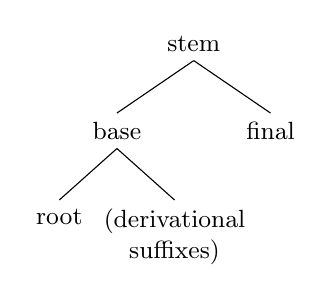
\begin{tikzpicture}[level distance=2.5em,
		sibling distance=8em,
		parent anchor=south,
		child anchor=north,
		anchor=north,
		align=center]
		\small
		\node{stem}
		child[sibling distance=6em]
		{node {base} edge from parent[solid]
			child[sibling distance=4.5em]
			{node {root} edge from parent[solid]}	
			child[sibling distance=4.5em]
			{node {(derivational\\suffixes)} edge from parent[solid]}
		}		
		child[sibling distance=6em]
		{node {final} edge from parent[solid]}
		
		;
		\end{tikzpicture}
		\captionabove{Hierarchical structure of the verb}\label{HierarchicalStructureVerb} 
	\end{center}
\end{figure} 

A number of verbs with initial /i/ are formally \isi{reflexive} verbs, that is, they are preceded by the reflexive object marker \textit{i}- (\sectref{Reflexive}). However, with some of these the reflexive semantics has become obscured and there may not exist a corresponding stem without the reflexive marker. There are at least two diagnostic criteria regarding the status of initial /i/. First, object prefixes do not count as stem syllables. Trisyllabic formal reflexives are thus treated as disyllabic in the formation of the perfective stem (see \sectref{Imbrication}).\is{imbrication}
\begin{exe}
	\ex
	\begin{tabbing}
		\textit{i-nogon-e!}x\=`turn (sthg.) upside down!'x\= > \textit{ikifiifye}x\=\kill
		\textit{itoga}\>`mount (horse, donkey)'\> > \textit{itogile}\>(not *\textit{itwige})\\
		\textit{ikifya}\>`do your best'\> > \textit{ikifiifye}\>(not *\textit{ikiifye})
	\end{tabbing}
\end{exe}

Second, any object prefix other than first person singular triggers a final vowel -\textit{e} in the imperative\is{mood!imperative} (\sectref{Imperative}) (\ref{exReflexiveFinalE}). Verbs in which initial /i/ is part of the stem have -\textit{a} (\ref{exInitialIStem}),
\begin{exe}
	\ex\label{exReflexiveFinalE}
	\begin{tabbing}
		\textit{i-nogon-e!}x\=`turn (sthg) upside down!'x\= > \textit{ikifiifye}x\=\kill
		\textit{i-jʊʊl-e!}\>`work hard!'\>(not *\textit{ijʊʊla})\\
		\textit{i-nogon-e!}\>`think!'\>(not *\textit{inogona})
	\end{tabbing} 
	\ex\label{exInitialIStem}
	\begin{tabbing}
		\textit{i-nogon-e!}x\=`turn (sthg) upside down!'x\=> \textit{ikifiifye}x\kill
		\textit{inamika!}\>`turn (sthg) upside down!'\\
		\textit{igʊla!}\>`open!'
	\end{tabbing}
\end{exe}

The final slot of the stem is obligatory and by default is occupied by the final vowel (\textsc{fv}) -\textit{a}, except for certain TMA paradigms and the defective verbs \textit{lɪ} and \textit{tɪ} (Chapter \ref{DefectiveVerbsCopulae}). Following Bantuist tradition, throughout the rest of this study verbs are listed as stems, except when explicitly making reference to hierarchically lower structures. Note that the verb stem is generally not a possible morphological word in Nyakyusa.\footnote{The exception is the imperative (\sectref{Imperative}),\is{mood!imperative} for those verbs that can figure in this paradigm and are not monosyllabic.}
\is{root|)}\is{base|)}\is{stem|)}
 \chapter{Verbal Derivation}\label{VerbalDerivation}
\is{derivation|(}
\section{Introduction}
Verbal derivation in Nyakyusa is accomplished by means of several devices. The most frequent is the use of derivational suffixes. These are also known as verbal extensions in Bantu studies \citep{SchadebergT2003a} and are common in the postulated Niger-Congo phylum \citep{HymanL2007}. The canonical verbal extension has the shape\mbox{-VC}, with the exception of the passive and causative extensions (\mbox{-V} and \mbox{-VCV}). While some verbal extensions, e.g. the applicative,\is{applicative} are highly productive, others like the \isi{tentive} can be segmented on the basis of their shape and meaning, but are not used productively to derive new verbs. Between these two extremes lie other extensions whose productivity is harder to determine as there seems to be a close interaction with verbal semantics (see \citealt{FleischA2000}). In these cases productivity is described on a tentative basis.

Verbal derivation by means of derivational suffixes is cyclic: once a derived verbal base has acquired a special or idiosyncratic meaning, this functions as the point of departure for subsequent derivations. 
\begin{exe}
\ex
\begin{tabbing}
 > \= > \= > \=\kill
\textit{fuma}\\
\lq come from'\\
 > \textit{fum\textbf{uk}a} \\
\>\lq be(come) known, famous' (separative)\\
\> > \textit{fum\textbf{usy}a}\\
\> \>\lq announce' (separative + causative)\\
\>\> > \textit{fum\textbf{usigw}a}\\
\>\>\> \lq be announced' (separative + causative + passive)
\end{tabbing}
\end{exe}

Verbal derivations cover a set of functions that can be subsumed under valency changing operations, semantic alternations, aktionsart\is{aktionsart} (see \sectref{Aktionsart}) and alternations in Aristotelian aspect\is{aspect!Aristotelian} (see \sectref{AristotelianAspect}). Some devices express a combination of these functions.

This chapter begins with an account of morphophonological processes affecting verbal extensions (\sectref{MorphophonologyOfVerbalExtension}), followed by a section on the form and function of each verbal extension (\sectref{Causative1}--\ref{extensive}). The treatment of the less productive extensions includes observations on lexical co-occurrences that are derived forms from the same root (commutations). Thereafter the combinations of verbal extensions are dealt with in more detail, including their respective order and some cases of specialized combinations (\sectref{CombinationOfVerbalExtensions}). Following the verbal extensions, denominal verb bases are dealt with (\sectref{Denominal}). Lastly, there is a note on partially reduplicated\is{reduplication} verbs (\sectref{PartialReduplication}).
\section{Verbal extensions}
\subsection{Morphophonology of verbal extensions}
\label{MorphophonologyOfVerbalExtension}
Verbal extensions in Nyakyusa are subject to two progressively operating processes affecting the degree of vowel opening: vowel height harmony and high vowel raising. 
\subsubsection{Vowel height harmony}\label{VowelHarmony} 
\is{vowels!vowel height harmony|(}
The verbal extensions with an underlying front vowel /ɪ/ surface with mid vowel /e/ following a syllable containing mid vowels /e, o/. 
The examples in (\ref{exVHHfront}) illustrate this for the applicative extension (only one possible reading given for each example).
\begin{exe}
\ex \label{exVHHfront}
\begin{tabbing}
\textit{bʊʊkɪla}x\=`measure with'x\= < \textit{bʊʊka}x\=\kill%Unsinn, fuer Tabulatoren
\textit{fikɪla}\>`arrive at'\> < \textit{fika}\>`arrive'\\
\textit{pɪmɪla}\>`measure with'\> < \textit{pɪma}\>`weigh, measure'\\
\textit{temela}\>`cut with'\> < \textit{tema}\>`cut' \\
\textit{jabɪla}\>`give off to'\> < \textit{jaba}\>\lq divide; distribute'\\
\textit{bopela}\>`run to'\> < \textit{bopa}\>`run'\\
\textit{bʊʊkɪla}\>`go to'\> < \textit{bʊʊka}\>`go (to)'\\
\textit{guulɪla}\>`wait for'\> < \textit{guula}\>`wait'
\end{tabbing}
\end{exe}

A similar rule applies to extensions beginning with the back vowel /ʊ/. The separative extensions -\textit{ʊl} and -\textit{ʊk} occur as -\textit{ol} and -\textit{ok} following a syllable with /o/ (but not /e/). They surface as -\textit{ul}/-\textit{uk} following a syllable with the high back vowel /u/. That is, front and back vowels are treated asymmetrically. Previous discussions of vowel harmony in Nyakyusa (e.g. \citealt{MwangokaNVoorhoeveJ1960b}; \citealt{LabroussiC1998}; \citealt{HymanL1999}) did not notice the raising of /ʊ/ to /u/. This rule of high vowel rising seems to be the expression of a more general constraint against stem-internal /*uCʊ/. These rules are illustrated in (\ref{exVHHback}) for the separative transitive extension. 
\begin{exe}
\ex \label{exVHHback}
\begin{tabbing}
\textit{niembʊla}x\=`disentangle'x\= < \textit{niemba}x\=\kill%Unsinn fuer Tabulatoren
\textit{kingʊla}\>`uncover'\> < \textit{kinga}\>`cover' \\
\textit{pɪndʊla}\>`convert'\> < \textit{pɪnda}\>`bend; wrap'\\
\textit{niembʊla}\>`disentangle'\> < \textit{niemba}\>`wrap up'\\
\textit{matʊla}\>`demolish'\> < \textit{mata}\>\lq plug, stop up'\\
\textit{bonola}\>`pay off'\> < \textit{bona}\>`see'\\
\textit{tʊngʊla}\>`pick'\> < \textit{tʊnga}\>`hang; string together'\\
\textit{fumbula}\>`solve'\> < \textit{fumba}\>`enclose in mouth or hands'
\end{tabbing}
\end{exe}

In principle, the rules of vowel harmony apply to all verbal extensions in question. (\ref{ruleVHH}) gives a formalized account. Extensions containing /i/ or /a/, such as the passive or the reciprocal, do not change their vowel quality. 

\begin{exe}
\ex \label{ruleVHH}
\phonc{ɪ}{e}{\oneof{
\mbox{e C \phold} \\
\mbox{o C \phold}}}
\\
\phonl{ʊ}{o}{o C} \\
\phonl{ʊ}{u}{u C}
\end{exe}

\label{VHHMonosyllabicVerbs} The shape of the verbal extensions subject to vowel height harmony on monosyllabic roots is not predictable in a straightforward fashion, at least in synchronic terms. (\ref{MonosyllabicAPPL}) lists the applicative forms of monosyllabic verbs together with their \ili{Proto-Bantu} forms.\footnote{Defective \textit{lɪ} and \textit{tɪ} do not take derivational suffixes.} 
\begin{exe} 
\ex
\begin{xlist} \label{MonosyllabicAPPL}
\ex 
\begin{tabbing}
\textit{mwa}x\=(*mò)x\=`be plenty (esp. fish)'x\=\kill%semantisch unsinnige Zeile, aber fuer Tabulatoren
\textit{pa}\>(*pá)\>`give'\> > \textit{peela}\\
\textit{ja}\>(*gɪ̀)\>`be(come)'\> > \textit{jɪɪla}
\end{tabbing}
\ex \begin{tabbing}
\textit{mwa}x\=(*mò)x\=`be plenty (esp. fish)'x\=\kill%semantisch unsinnige Zeile, aber fuer Tabulatoren
\textit{fwa}\>(*kú)\>`die'\> > \textit{fwɪla}\\
\textit{gwa}\>(*gʊ̀)\>`fall'\> > \textit{gwɪla}\\
\textit{kwa}\>(*kó)\>`pay dowry'\> > \textit{kwela} \\
\textit{lwa}\>(*dʊ̀)\>`fight'\> > \textit{lwɪla}\\
\textit{mwa}\>(*mò)\>`shave'\> > \textit{mwela}\\
\textit{nwa}\>(*ɲó)\>`drink'\> > \textit{nwela}\\
\textit{swa}\>(*tu?)\>`spit; forgive'\> > \textit{swela}\\
\textit{twa}\>(*tó?)\>`be plenty (esp. fish)'\> > \textit{twɪla}
\end{tabbing}
\ex
\begin{tabbing}
\textit{mwa}x\=(*mò)x\=`be plenty (esp. fish)'x\=\kill%semantisch unsinnige Zeile, aber fuer Tabulatoren
\textit{kya}\>(*ké)\>`dawn; cease to rain'\> > \textit{kyela}\\
\textit{lya}\>(*lɪ́)\>`eat'\> > \textit{lɪɪla}\\
\textit{nia}\>(*nè)\>`defecate'\> > \textit{niela}\\
\textit{pya}\>(*pɪ́)\>`be(come) burnt'\> > \textit{pɪɪla}\\
\textit{sya}\>(*cè)\>`grind'\> > \textit{syela}
\end{tabbing}
\end{xlist}
\end{exe}

As can be gathered, \textit{pa} is treated as underlying \textit{pa-a} for derivational purposes. With all other monosyllabic roots, the surface glide is retained, unless the sequence is /*ɪ-ɪ/. The vowel quality of the derivational suffix as such is conditioned by the historic root vowel and shows the same alternations as with longer verbs. The only exceptions are \textit{twa} `be plenty (esp. of fish)', whose origin in \textit{*tó} `bite' is merely tentative, and \textit{swa} \lq spit; forgive' < *\textit{tú} \lq spit', where *\textit{fwa} would be expected according to the rules of diachronic phonology.
\is{vowels!vowel height harmony|)}
\subsubsection{High vowel raising}\label{HighVowelRaising}
\is{vowels!high vowel raising|(}
Two further and related processes affect the quality of vowels in verbal extensions. What both have in common is the raising of the second degree vowels /ɪ, ʊ/ to the first degree /i, u/. First, the underlying vowels of verbal extensions are raised to first degree vowels when following the palatal nasal,\footnote{This seems to be the expression of a more general constraint against stem-internal /*nyɪ, nyʊ/, cf. also nominal stems like \textit{unyu} \lq salt' < PB\textit{*jɪ́nyʊ̀}.} as illustrated in (\ref{exVowelRaisingAfterPalatalNasal}) with the \isi{applicative} (-\textit{ɪl}), \isi{neuter} (-\textit{ɪk}), \isi{causative}\textsubscript{2} (-\textit{ɪsi}) and the \isi{separative} (-\textit{ʊl}/-\textit{ʊk}) extensions.

\begin{exe}
\ex \label{exVowelRaisingAfterPalatalNasal}
\begin{tabbing}
\textit{tuuny\textbf{u}ka}x\=(\degree tuuny-ʊk-a)x\=`disencourage'x\= < \textit{tuunya}x\=\kill
\textit{many\textbf{i}la}\>(\degree many-ɪl-a)\>`learn'\> < \textit{manya} \lq know'\\
\textit{many\textbf{i}ka}\>(\degree many-ɪk-a)\>`be known'\\
\textit{many\textbf{i}sya}\>(\degree many-ɪsi-a)\>`teach'\\
\textit{kany\textbf{i}sya}\>(\degree kany-ɪsi-a)\>`fill up, stuff'\>< \textit{kanya}\>`tread on'\\
\textit{tuuny\textbf{i}la}\>(\degree tuuny-ɪl-a)\>`throw at'\> < \textit{tuunya}\>`throw'\\
\textit{tuuny\textbf{u}ka}\>(\degree tuuny-ʊk-a)\>`fall (from)'\\
\textit{kiny\textbf{u}la}\>(\degree kiny-ʊl-a)\>`disencourage'\> < \textit{kinya} \>`hit'
\end{tabbing}
\end{exe}

This rule does not apply when the vowel in question is affected by vowel height harmony\is{vowels!vowel height harmony} (\ref{exVowelPalatalRaisingBlockedByVHH}). Also, only the directly adjacent vowel is subject to high vowel raising (\ref{exVowelRaisingPalatalNoSpreading}).

\begin{exe}
\ex \label{exVowelPalatalRaisingBlockedByVHH} 
\begin{tabbing}
\textit{toony\textbf{e}sya}x\=`break, wreck; harvest corn'x\=< \textit{keenya}x\=\kill%Unsinnszeile fuer Tabulatoren
\textit{toony\textbf{e}sya}\>`cause to fall or drip'\> < \textit{toonya}\>`drip, ooze'\\ 
\textit{keeny\textbf{e}sya}\>`insult, shout at'\> < \textit{keenya}\>`insult'\\
\textit{kony\textbf{o}la}\>`break, wreck; harvest corn'\> < *\textit{kóny}\>`fold, bend, twist'\\
\textit{kony\textbf{o}ka}\>`break (intr.)'
\end{tabbing}
\ex\label{exVowelRaisingPalatalNoSpreading}
\begin{tabbing}
\textit{keeny\textbf{e}sya}x\=`break, wreck; harvest corn'x\=< \textit{keenya}x\=\kill%Unsinnszeile fuer Tabulatoren
\textit{many\textbf{i}l\textbf{ɪ}la}\>`know (much)'\> < \textit{manya}\>`know'\\
\textit{piny\textbf{i}l\textbf{ɪ}la}\>`tie up, bind repeatedly'\> < \textit{pinya}\>`bind; detain; fix'\\
\textit{keny\textbf{u}l\textbf{ɪ}la}\>`add too much; oversalt'
\end{tabbing}
\end{exe}

The underlying second degree vowels /ɪ, ʊ/ of verbal extensions are also realized as first degree /i, u/ when they follow a sequence of low vowel /a/ plus the coronal or bilabial nasals /n/ or /m/. Examples are given in (\ref{exHighVowelRaisingAfterReciprocalPositional}) for the extensions in question when following the \isi{reciprocal} and \isi{positional} extensions, while (\ref{exHighVowelRaisingAfteranmRootfinal}) illustrates this for root-final sequences.\footnote{Again, this seems to be the expression of a more general phonotactic constraint: Regardless of syntactic class, no stem containing /an, am/ followed by a second degree vowel is attested in the data.}

\begin{exe}
\ex \label{exHighVowelRaisingAfterReciprocalPositional}
\begin{tabbing}
\textit{swigan\textbf{i}ka}x\=(\degree swig-an-ɪk-a)x\=\lq turn upside down' \= < \textit{batama}x\=`be silent'\kill%unsinnige Zeile, fuer Tabs
\textit{koman\textbf{i}la}\>(\degree kom-an-ɪl-a)\>`fight for'\> < \textit{koma}\>`hit'\\
\textit{swigan\textbf{i}ka}\>(\degree swig-an-ɪk-a)\>`wonder (much)' \> < \textit{swiga}\>`wonder' \\
\textit{sulam\textbf{i}ka}\>(\degree sulam-ɪk-a)\>`turn upside down'\> < \textit{sulama}\>`bend, droop'\\
\textit{batam\textbf{i}sya}\>(\degree batam-ɪsi-a)\>`silence, caress'\> < \textit{batama}\>`be silent'
\end{tabbing}
\ex
\label{exHighVowelRaisingAfteranmRootfinal}
\begin{tabbing}
\textit{swigan\textbf{i}ka}x\=(\degree swig-an-ɪk-a)x\=`turn upside down' \= < \textit{batama}x\=`be silent'\kill%unsinnige Zeile, fuer Tabs
\textit{gan\textbf{i}la}\>(\degree gan-ɪl-a)\>`love + \textsc{appl}'\> < \textit{gana} \>`love'\\
\textit{gan\textbf{i}sya}\>(\degree gan-ɪsi-a)\>`cause to love'
\\\textit{kaan\textbf{i}ka}\>(\degree kaan-ɪk-a)\>`dispute'\> < \textit{kaana}\> `refuse'\\
\textit{kaan\textbf{i}la}\>(\degree kaan-ɪl-a)\>`refuse'\\
\textit{kaan\textbf{i}sya}\>(\degree kaan-ɪsi-a)\>`forbid'\\
\textit{kam\textbf{i}la}\>(\degree kam-ɪl-a)\>`milk + \textsc{appl}'\> < \textit{kama}\>`milk, squeeze'
\\ \textit{kam\textbf{u}la}\>(\degree kam-ʊl-a)\>`squeeze out'
\\ \textit{lam\textbf{u}la}\>(\degree lam-ʊl-a)\>`stop fight; judge'\> *\textit{dàm-ʊd}\>`settle dispute'
\\ \textit{saam\textbf{i}la}\>(\degree saam-ɪl-a)\>`move + \textsc{appl}'\> < \textit{saama}\>`move, migrate'
\\ \textit{saam\textbf{i}sya}\>(\degree saam-ɪsi-a)\>`transfer; displace'
\end{tabbing}
\end{exe}

Again, only the directly adjacent vowel undergoes raising:
\begin{exe}
\ex \label{exNoSpreadingAfterRaisinganmn}
\begin{tabbing}
\textit{saam\textbf{i}k\textbf{ɪ}sya}x\=(\degree fwan-ɪkɪsi-a)x\=`migrate + \textsc{intns}'x\= < \textit{sanuka}x\=`move, migrate'\kill%unsinnszeile, fuer tabulatoren
\textit{fwan\textbf{i}k\textbf{ɪ}sya}\>(\degree fwan-ɪkɪsi-a)\>`compare'\> < \textit{fwana}\>\lq resemble'
\\\textit{kaan\textbf{i}l\textbf{ɪ}la}\>(\degree kaan-ɪlɪl-a)\>`refuse +\textsc{intns}'\> < \textit{kaana}\>`refuse'
\\\textit{saam\textbf{i}k\textbf{ɪ}sya}\>(\degree saam-ɪkɪsi-a)\>`transfer; exile to'\> < \textit{saama}\>`move, migrate'
\\\textit{saam\textbf{i}l\textbf{ɪ}la}\>(\degree saam-ɪlɪl-a)\>`migrate + \textsc{intns}'
\\\textit{san\textbf{u}k\textbf{ɪ}la}\>(\degree sanuk-ɪl-a)\>`turn to'\> < \textit{sanuka}\>\lq alter'\\
\textit{am\textbf{u}l\textbf{ɪ}sya}\>(\degree amul-ɪsi-a)\>`make answer'\>< \textit{amula}\>`answer'
\end{tabbing}
\end{exe}

The examples in (\ref{exNoRaisingAC}) show that other /aC/ sequences do not induce raising of the second degree vowels.\footnote{A few combinations are not attested in the data: /aŋɪ, afɪ, afu/. The lack of the first is due to the scarcity of the velar nasal, while the lack of the other two stems from the fact that the bilabial fricative /f/ has its main diachronic source in sequences of \ili{Proto-Bantu} plosives followed by a first degree vowel.} The examples in (\ref{exNoRaisingVN}) show that other /VN/ sequences likewise do not induce high vowel raising (but see above on the effects of the palatal nasal, and below on the sequence /mu/).
\clearpage

\begin{exe}
\ex\label{exNoRaisingAC}
\begin{tabbing}
\textit{nangɪsya}x\=`be(come) unravelled'xxx\=\textit{nangɪsya}x\=\kill
/ap, at, ak/ \>\> /amb, and, aŋg/ \\
\textit{paapɪla}\>`give birth + \textsc{appl}' \> \textit{bambɪka}\>`arrange in line'\\
\textit{tapʊka}\>`separate'\>\textit{sambʊka}\>`rebel'\\
\textit{ʊbatɪla}\>`embrace'\>\textit{andɪsya}\>`establish; repeat'\\
\textit{latʊla}\>`rip' \> \textit{andʊla}\>`change; convert'\\
\textit{pakɪla}\>`load + \textsc{appl}' \> \textit{nangɪsya}\>`show'\\
\textit{sakʊka}\>`reappear' \> \textit{pangʊla}\>`dismantle'\\
/aβ̞, al, aɟ, aɰ/\>\> /as, ah/\\
\textit{laabɪla}\>`get up early; be early' \> \textit{lasɪla}\>`stab + \textsc{appl}'\\
\textit{abʊla}\>`release; open' \> \textit{pasʊka}\>`burst'\\
\textit{malɪka}\>`(be) finish(ed) (intr.)' \> \textit{hahɪla}\>\lq propose + \textsc{appl}'\\
\textit{saalʊka}\>`be(come) unravelled' \> /aŋ/\\
\textit{baajɪka}\>`kick + \textsc{appl}' \> \textit{kang'ʊla}\>`remove stopper'\\
\textit{tajʊka}\>`break up (intr.)' \\
\textit{bagɪla}\>\lq be able; suit'\\
\textit{pagʊka}\>`fall apart'
\end{tabbing}
%I have tried to solve the above with multicols, but had no success
\ex
\label{exNoRaisingVN}
\begin{tabbing}
\textit{nangɪsya}x\=\kill
/V$\neq$a\{n, m\}/\\
\textit{pɪmɪla}\>\lq measure + \textsc{appl}'\\
\textit{inɪsya}\>\lq dirty (tr.)'\\
\textit{inʊla}\>\lq lift'\\
\textit{timɪla}\>\lq rain + \textsc{appl}'\\
\textit{ʊmɪla}\>\lq dry + \textsc{appl}'
\end{tabbing}
\end{exe}

A formalized account of the rules of high vowel raising is given in (\ref{ruleVowelRaisingAfterPalatalNasal}, \ref{exRuleHigVowelRaisingAfteranm}).
\begin{exe}
\ex \label{ruleVowelRaisingAfterPalatalNasal}
\phonl{
	\oneof{
	\mbox{ɪ} \\
	\mbox{ʊ}}
	}
	{\oneof{
	\mbox{i} \\
	\mbox{u}}
	}
	{ny}
\ex \label{exRuleHigVowelRaisingAfteranm}
\phonl{
	\oneof{
	\mbox{ɪ} \\
	\mbox{ʊ}}
	}
	{\oneof{
	\mbox{i} \\
	\mbox{u}}}
{a\{n, m\}}
\end{exe}

Lastly, in a few stems the sequence /mu/ is found in contexts where it cannot be accounted for by the above rules (\ref{exMuStem}). This seems to be the expression of a general phonotactic constraint against /mʊ/.\footnote{This kind of constraint against certain CV sequences may be more widespread in Bantu. \citet{BennettWGLeeSJ2015} describe in detail how the sequence /li/ is strongly dispreferred in \ili{Tsonga} S53.} While the latter sequence may be the outcome of vowel coalescence between the vowel of a prefix and a vowel-initial stem (\sectref{HiatusSolution})\is{vowels!hiatus solution}, no stem or affix containing it is attested.\footnote{Note that this constraint alone cannot explain the raising of the front vowel /ɪ/ after \mbox{/a\{m, n\}/}, nor can it explain the raising of /ʊ/ after /an/, as /mɪ, nɪ, nʊ/ are licensed stem-internal syllables.}

\begin{exe}
\ex \label{exMuStem}
\begin{tabbing}
\textit{nyenyemusya}x\=`speak much'x\=\kill
\textit{lendemuka}\>`crack'
\\\textit{nyenyemusya}\>`excite'
\\\textit{telemuka}\>`slip'\> < *\textit{tèdɪmʊk} 
\\\textit{syelemuka}\>`slip'\> < *\textit{tɪ̀edɪmʊk}
\\\textit{tyemula}\>`sneeze'\> < *\textit{tɪ́emʊd}
\\\textit{tyesemula}\>`sneeze'
\end{tabbing}
\end{exe}

\is{vowels!high vowel raising|)}
\subsection{Causative 1} \label{Causative1} 
\is{causative|(}
The verbal suffix -\textit{i} serves to derive causative verbs. Before turning to a closer examination of its function, some formal aspects require discussion.

Synchronically speaking, the vowel of this extension is not directly observable; instead it surfaces as the glide /y/. It is interpreted as -\textit{i} because of the morphophonological changes it induces, which in diachronical terms go back to a first degree front vowel. Lingual plosives and approximants preceding this causative suffix are spirantized\is{spirantization} to /s/, while their labial counterparts change to /f/. This rule, which constitutes a typical case of Bantu \isi{spirantization} (see \citealt{BoestonK2008}), is given (\ref{RuleSpirantizationCaus1}) and illustrated in (\ref{exSpirantizationCaus1}).
\begin{exe}  
\ex Spirantization\is{spirantization} triggered by causative -\textit{i}\label{RuleSpirantizationCaus1}
\begin{xlist}
\ex \phonr{\{ t, l, j, k, g \}}{s}{i}
\ex \phonr{\{ p, b \}}{f}{i}
\end{xlist}
\ex\label{exSpirantizationCaus1} 
\begin{tabular}[t]{llll}
\textit{bosya}&`cause to rot'& < \textit{bola}&`rot'\\
\textit{sesya}&`make laugh'& < \textit{seka}&`laugh'\\
\textit{osya}&\lq bathe (tr.); baptize'& < \textit{oga}&`bathe (intr.)'\\
\textit{pyʊfya}&`warm, heat up'& < \textit{pyʊpa}&`get warm'\\
\textit{sofya}&`loose; mislead'& < \textit{soba}&`be lost; be wrong'
\end{tabular}
\end{exe}

\largerpage %long distance for 'moo'
When prenasalized plosives are spirantized, the preceding vowel becomes long (\ref{exCausative1NC}).\footnote{This can be analyzed either as retention of the compensatory lengthening triggered by the NC cluster or as subsequent deletion of the word-internal non-syllabic nasal plus compensatory lengthening, cf. the first person singular object prefix\is{object marker} (\sectref{SubjectConcordsParticipants}).} The \isi{causative} -\textit{i} followed by passive\is{passive!productive} -\textit{igw} surfaces with a short vowel;\is{vowels!length} see p.\nobreakspace\pageref{exCausativePassiveShortVowel} in \sectref{Passive}.

\begin{exe}
\ex\label{exCausative1NC}
\begin{tabbing}
\textit{joosya}x\=\lq make pass, pass through; allow'x\= < \textit{kɪnda}x\=\kill %nonsense line for tabs
\textit{kɪɪsya} \>\lq make pass, pass through; allow' \> < \textit{kɪnda} \> \lq pass'\\
\textit{joosya} \>`elope with girl; lose' \> < \textit{jonga} \> `run away'
\end{tabbing}
\end{exe}

When serving as a typical causative, this extension increases the valency of the verb by one. It introduces an agent that causes the act of the underlying verb and demotes the original subject to an object. The following examples illustrate this.
\begin{exe}
\ex
\begin{tabular}[t]{llll}
\textit{elʊsya} & \lq clean, rinse' & < \textit{elʊka} & \lq become white, clean'\\
\textit{fulasya} & \lq hurt (tr.)' & < \textit{fulala} & \lq (be)come hurt'\\
\textit{isʊsya} & \lq fill' & < \textit{isʊla} & \lq (be)come full'\\
\textit{sumusya} & \lq make stand up, get up' & < \textit{sumuka} & \lq get up, depart'\\
\textit{kusya} & \lq blow away' & < \textit{kula} & \lq blow (intr.), drift'
\end{tabular}
\end{exe}

Causative -\textit{i} has developed idiosyncratic readings with a number of verbs, but it is no longer productive in the present-day language. These issues are dealt with in more detail in \sectref{TwoCausatives}.
\subsection{Causative 2}\label{Causative2}
The extension -\textit{ɪsi} (allomorphs -\textit{esi}, -\textit{isi}, see \sectref{MorphophonologyOfVerbalExtension},) serves to derive causative verbs. \mbox{-\textit{ɪsi}} is the only causative extension used with monosyllabic verbs and verbs ending in the palatal nasal (\ref{exCaus2MonoPalatal}). It is also the only productive causative in Nyakyusa; see \sectref{TwoCausatives} for discussion.

\begin{exe}
\ex\begin{xlist}
\ex \label{exCaus2MonoPalatal}Causatives of monosyllabic verbs:
\begin{tabbing}
\textit{kuunya}x\=`bind; detain; fix'x\= > \textit{kunuyisya}x\=\kill%Unsinnszeile für Tabulatoren 
\textit{gwa}\>`fall'\> > \textit{gwɪsya}\>`overturn, throw down'\\
\textit{lwa}\>`fight'\> > \textit{lwɪsya}\>`cause to fight'\\
\textit{nwa}\>`drink'\> > \textit{nwesya}\>`make drink, water'\\
\textit{lya}\>`eat'\> > \textit{lɪɪsya}\>`feed'\\
\textit{sya}\>`grind'\> > \textit{syesya}\>`make grind'%needs checking
%evtl weiteres bsp
\end{tabbing}
\ex Causatives of bases ending in -\textit{ny}:
\begin{tabbing}
\textit{kuunya}x\=`bind; detain; fix'x\= > \textit{kuunyisya}x\=\kill%Unsinnszeile für Tabulatoren 
\textit{manya}\>`know'\> > \textit{manyisya}\>`teach'\\
\textit{pinya}\>`bind; detain; fix`\> > \textit{pinyisya}\>`make bind'\\
\textit{kuunya}\>`push, bump'\> > \textit{kuunyisya}\>`make push, bump'
\end{tabbing}
\end{xlist}
\end{exe}

The suffix -\textit{ɪsi} may be analysed as consisting of two morphemes -\textit{ɪs}-\textit{i}. In combination with the reciprocal/associative\is{reciprocal} it often surfaces as -\textit{ɪs}-\textit{an}-\textit{i}; see also \sectref{ReciprocalAndCausative}. Also note that any causative followed by the passive \mbox{-\textit{igw}}\is{passive!productive} surfaces with a short vowel;\is{vowels!length} see p.\nobreakspace\pageref{exCausativePassiveShortVowel} in \sectref{Passive}.
\begin{exe}
\ex
\begin{tabular}[t]{llll}
\textit{lwɪsania}&`make fight each other'& < \textit{lwa}&`fight'\\
\textit{sobesania}&`loose each other'& < \textit{soba} & \lq be lost'
\end{tabular}
\end{exe}

Causative\textsubscript{2} -\textit{ɪsi} increases the valency of the verb by one, introducing an agent-causer and demoting the original subject to an object. See (\ref{exShortCausativeLexicalized}--\ref{exCausative2Productive}) in \sectref{TwoCausatives} for numerous examples. Causative\textsubscript{2} can further be used to add an intensive, evaluative meaning without changing the verb's argument structure (\ref{exCaus2Intensifying1}, \ref{exCaus2Intensifying2}). Such an intensifying use of the causative has also been reported for neighbouring \ili{Ndali} \citep[73f]{BotneR2003} and other Bantu languages such as \ili{Chewa} N20 \citep[78f]{IntensiveChichewa}, \ili{Bemba} M42 \citep[83--92]{vanSambeekJ1955} and \ili{Kalanga} S16 \citep[397]{MathangwaneJ2001}. For a typological perspective see \citet{KittilaeS2009}.
\begin{exe}
\ex \label{exCaus2Intensifying1}\gll i-kʊ-mmw-amul-ɪsy-a\\
1-\textsc{prs}-1-answer-\textsc{caus}-\textsc{fv}\\
\glt `1. S/he makes him/her answer.'\\
`2. S/he answered him/her snottily.' [ET]
\ex \label{exCaus2Intensifying2}\gll i-kʊ-ba-hah-ɪsy-a a-ba-kiikʊlʊ\\
1-\textsc{prs}-2-persuade-\textsc{caus}-\textsc{fv} \textsc{aug}-2-woman\\
\glt `He goes around proposing to women.' [ET]
\end{exe}

\subsection{The relationship between the two causatives}
\label{TwoCausatives}
As was seen in the preceding sections, Nyakyusa has two causative morphemes: -\textit{i} and -\textit{ɪsi}. Their distribution is partly conditioned by phonology. Only -\textit{ɪsi} applies with monosyllabic verbs and following /ɲ/. These phonological contexts aside, in the variety described by \citet{SchumannK1899} and \citet{EndemannC1914}, causative\textsubscript{1} -\textit{i} figures as the more productive morpheme of the two. For the present-day language, however, \citet{LabroussiC1999} observes that causative\textsubscript{2} -\textit{ɪsi} has widely replaced causative\textsubscript{1} -\textit{i}. Labroussi's observations are corroborated in the data. First, in a number of cases, causative\textsubscript{1} -\textit{i} is lexicalized with idiosyncratic meanings, whereas causative\textsubscript{2} -\textit{ɪsi} yields a more transparent meaning and syntax. (\ref{exShortCausativeLexicalized}) illustrates a few of these.

\begin{exe}
\ex \label{exShortCausativeLexicalized}
\begin{tabbing}
\textit{taama}x\=\lq recover; escape'x\= > \textit{taamisya}x\=\kill %nonsense line for tabs
\textit{kʊba} \> \lq beat; ring; play' \> > \textit{kʊfya} \> \lq cause trouble' not: \lq make beat'\\
\> \> > \textit{kʊbɪsya} \> \lq make beat, ring, play'\\
\textit{oga} \> \lq bathe (intr.)' \> > \textit{osya} \> \lq bathe (tr.); baptize'\\
\> \> > \textit{ogesya} \> \lq bathe (tr.)' not: \lq baptize'\\
\textit{pona} \> \lq recover; escape' \> > \textit{ponia} \> \lq greet, visit' not: \lq cure'\\
\> \> > \textit{ponesya} \> \lq cure, rescue'\\
\textit{syala} \> \lq remain' \> > \textit{syasya} \> \lq leave over' not: \lq make remain'\\
\> \> > \textit{syalɪsya} \> \lq make remain'\\
\textit{taama} \> \lq moo' \> > \textit{taamya} \> \lq trouble; persecute'\\
\>\>\>not: \lq make moo'\\
\> \> > \textit{taamisya} \> \lq make moo'
\end{tabbing}
\end{exe}

In other cases, both causatives are attested without any apparent difference in meaning. With most of these, there is a preference for the long causative\textsubscript{2}. However, with a few verbs, the short causative\textsubscript{1} is strongly preferred or is the only acceptable form (\ref{exPreferenceCaus1}). The data at hand suggest that this kind of lexicalization is particularly the case with verbs featuring the separative intransitive (\sectref{Separative}) and the extensive (\sectref{extensive}).

\begin{exe}
\ex \label{exPreferenceCaus1}\begin{tabbing}
\textit{hoboka}x\=\lq be(come) happy'x\= > \textit{hobokesya}x\=\kill %nonsene line for tabs
\textit{fulala}\> \lq be(come) hurt'\> > \textit{fulasya} \> \lq hurt (tr.)'\\
\textit{hoboka}\> \lq be(come) happy'\> > \textit{hobosya} \> \lq amuse\\
\> \> \hphantom{> }*\textit{hobokesya}\\
\textit{kalala}\> `be(come) angry' \> > \textit{kalasya} \> \lq enrage'\\
\> \> \hphantom{> }*\textit{kalalɪsya}\\
\textit{lɪla}\>i.a. \lq cry' \> > \textit{lɪsya} \> \lq make cry' (preferred)\\
\> \> > \textit{lɪlɪsya} \> \lq make cry'\\
\textit{pyʊpa}\> i.a. \lq get warm' \> > \textit{pyʊfya} \> \lq heat, warm up'\\
\> \> \hphantom{> }*\textit{pyʊpɪsya}
\end{tabbing} 
\end{exe}

Furthermore, causative\textsubscript{2} -\textit{ɪsi} is the only one which is applied productively (\ref{exCausative2Productive}). Causative\textsubscript{1} \mbox{-\textit{i}} was rejected with most roots, including a number of those listed by \citet{MeinhofC1966}[1910], \citet{SchumannK1899}, and \citet{EndemannC1914}.\footnote{\textit{hobokesya} is acceptable nevertheless as the applicativized causative. \citet{FelbergK1996} lists \textit{kalalɪsya} for the variety of the lake-shore plains,\is{dialects} so topological differences might also come into play. Some of these forms exist as causatives of other verbs: \textit{baasya} < \textit{baala} \lq increase, thrive', \textit{pɪɪsya} < \textit{pya} \lq be(come) burnt'. \citet{MwangokaNVoorhoeveJ1960c} list \textit{keesya} < \textit{keeta}, which was rejected by the speakers consulted for this study.} 

\begin{exe}
\ex \label{exCausative2Productive}
\begin{tabbing}
\textit{baaja}x\= \lq be(come) satisfied\lq x\= > \textit{keetesya}x \= \lq make cultivate'x\= \kill %Unsinnszeile für Tabulatoren
\textit{baaja} \> \lq kick' \> > \textit{baajɪsya} \> \lq make kick' \> not: *\textit{baasya}\\
\textit{bona} \> \lq see' \> > \textit{bonesya} \> \lq show' \> not *\textit{bonia}\\%ist auch eins aus alten Quellen
\textit{funja} \> \lq harvest' \> > \textit{funjɪsya} \> \lq make harvest' \> not: *\textit{fuusya}\\%dito
\textit{ikʊta} \> \lq be(come) satisfied' \> > \textit{ikʊtɪsya} \> \lq satisfy' \> not: *\textit{ikʊsya}\\
\textit{jaata} \> \lq walk' \> > \textit{jaatɪsya} \> \lq make walk' \> not: *\textit{jaasya}\\
\textit{jenga} \> \lq build' \> > \textit{jengesya} \> \lq make build' \> not: *\textit{jeesya}\\
\textit{keeta} \> \lq look, watch' \> > \textit{keetesya} \> \lq make look' \> not: *\textit{keesya}\\%ist eins von denen von endemann,schumann
\textit{lɪma} \> \lq cultivate' \> > \textit{lɪmɪya} \> \lq make cultivate' \> not: *\textit{lɪmya}\\
\textit{pɪɪja} \> \lq cook' \> > \textit{pɪɪjɪsya} \> \lq make cook' \> not: *\textit{pɪɪsya}
\end{tabbing}
\end{exe}

Lastly, causative\textsubscript{2} -\textit{ɪsi} is found with the same function as causative\textsubscript{1} -\textit{i} in the derivation of pluractionals\is{pluractional} (see \sectref{Pluractional}). It is also subject to the same templatic requirements as -\textit{i} in the formation of applicativized\is{applicative} causatives (\sectref{ApplicativizedCausatives}) and perfective stems (\sectref{Imbrication}),\is{imbrication} both of which can be diachronically traced back to \isi{spirantization} triggered by causative\textsubscript{1} \textit{-i}.

\citet{LabroussiC1999} regards the loss of productivity of causative\textsubscript{1} -\textit{i} as an epiphenomenon of the more general decline of \isi{spirantization} in Nyakyusa, which is also observed in the agent noun suffix -\textit{i}. The latter is lexicalized with spirantizing forms,\is{spirantization} but does not productively cause consonant mutation. What Labroussi does not consider is the fossilization of passive\is{passive!fossilized} *-\textit{ʊ} (\sectref{FossilizedPassive}), which has been replaced by the reflex of PB *-\textit{ibʊ} (\sectref{Passive}).\is{passive!productive} The alternation between these two was historically also triggered by phonological context \citep[78]{SchadebergT2003a}. Thus, apart from a general decline of spirantization,\is{spirantization} present-day Nyakyusa also shows a general preference for suffixes of the shape -VCV over -V.
\is{causative|)}
\subsection{Reciprocal/Associative}
\label{Reciprocal}\is{reciprocal|(}
The reciprocal/associative extension has the shape -\textit{an}. With some roots, this extension surfaces with a long vowel,\is{vowels!length} which is maintained in complex derivations (\sectref{CombinationOfVerbalExtensions}). The long allomorph is induced predominantly, but not exhaustively, by roots\is{root} of the shape (C)VNC.

\begin{exe}
	\ex \label{exReciprocalLong}
	Long reciprocals -\textit{aan}:
	\begin{xlist}
		\ex Following (C)VNC:
		\begin{tabbing}
			\textit{jʊʊgaanika}x\=\lq kill each other with blade'x\= < *\textit{bʊnga}x\=\kill%Unsinnszeile fuer Tabulatoren
			\textit{bʊngaana}\>`gather, be assembled'\> < *\textit{bʊ́nga} `gather up'\\
			\textit{lɪngaania}\>\lq explain; narrate'\> < \textit{lɪnga}\>`peep through'\\
			\textit{lʊngaana}\>`join together (intr.)'\>< \textit{lʊnga}\>`join; add spice'\\
			\textit{ongaana}\>`be together, be mixed'\> < \textit{onga}\>`suck'\\
			\textit{sangaana}\>\lq kill each other with blade'\> < \textit{sanga}\>\lq slaughter'\\
			\textit{tengaana}\>\lq settle; live in peace'\> < \textit{tenga}\>`make bed'
		\end{tabbing}
		\ex Following CV(V)C:
		\begin{tabbing}
			\textit{jʊʊgaanika}x\=\lq kill each other with blade'x\= < *\textit{bʊnga}x\=\kill%Unsinnszeile fuer Tabulatoren
			\textit{jʊʊgaania}\>`shake, aggitate'\\
			\textit{jʊʊgaanika}\>`tremble'\\
			\textit{kolaana}\>`grasp, hold e.o.; accuse e.o.'\> < \textit{kola}\>\lq grasp, hold' \\
			\textit{kolaania}\>`multitask'\\
			\textit{lekaana}\>`leave e.o.; release e.o.'\> < \textit{leka}\>\lq release; let'\\
			\textit{manyaana}\>`be(come) acquainted'\> < \textit{manya}\>`know'
		\end{tabbing}
	\end{xlist}
\end{exe}


However, not all (C)VNC roots\is{root} have the long allomorph (\ref{exReciprocalShortNC}). Further, one minimal pair -\textit{an} vs. -\textit{aan} is attested (\ref{exMPReciprocalsLongShort}).\is{vowels!length}
\pagebreak
\begin{exe}
	\ex \label{exReciprocalShortNC} Short reciprocal -\textit{an} following (C)VNC:
	\begin{tabbing}
		\textit{komaana}x\=`follow e.o.; depend upon e.o.'x\= < \textit{manya}x\=\kill%unsinnszeile fuer tabulatoren
		\textit{andana}\>`be early'\> < \textit{anda}\>`start'\\
		\textit{kongana}\>`follow e.o.; depend upon e.o.'\> < \textit{konga}\>\lq follow'\\
		\textit{ningana}\>`give e.o.; be opposite e.o.'\> < \textit{ninga}\>`give'\\
		\textit{pɪngana}\>`debate, disagree'\> < \textit{pɪnga}\>`obstruct'
	\end{tabbing}
	\ex \label{exMPReciprocalsLongShort}
	\begin{tabbing}
		\textit{komaana}x\=`follow e.o.; depend upon e.o.'x\= < \textit{manya}x\=\kill%unsinnszeile fuer tabulatoren
		\textit{komana}\>`fight'\> < \textit{koma}\>`hit' \\
		\textit{komaana}\>`hold a meeting'
	\end{tabbing}
\end{exe}

Having broached the formal issues of the reciprocal/associative, its function can now be examined. The reciprocal/associativ is commonly used with transitive verbs and yields a reciprocal action. The verb's valency in this case decreases by one.

\begin{exe}
	\ex
	\begin{tabbing}
		\textit{tʊʊlana}x\=\lq divide amongst each other'x\= < \textit{tʊʊla}x\=\kill%unsinnszeile fuer tabulatoren
		\textit{sekana} \> \lq make fun of each other' \> < \textit{seka} \> \lq laugh (at)'\\
		\textit{tʊʊlana} \> \lq help each other' \> < \textit{tʊʊla} \> \lq help'\\
		\textit{titana}\> \lq pinch each other' \> < \textit{tita} \> \lq pinch'
	\end{tabbing} 
\end{exe}

Another reading of the reciprocal/associative is that of a joint action. Accordingly, valency remains unchanged:

\begin{exe}
	\ex\begin{tabbing}
		\textit{tʊʊlana}x\=\lq divide amongst each other'x\= < \textit{tʊʊla}x\=\kill%unsinnszeile fuer tabulatoren
		\textit{jabana}\>\lq divide amongst each other' \> < \textit{jaba} \> \lq divide; distribute'\\
		\textit{gonana}\>\lq sleep together, copulate' \> < \textit{gona} \> \lq rest, sleep'
	\end{tabbing}
\end{exe}

A closer look at examples (\ref{exReciprocalLong}, \ref{exReciprocalShortNC}) above shows that the reciprocal/associative often expresses a further range of related meanings in the area of middle voice \citep{KemmerS1993}. A preliminary classification, including some of the above examples, is given in the following:
\begin{exe}
	\ex\label{exReciprocalMiddle}\begin{xlist}
		\ex Verbs of being (dis-)connected:
		\begin{tabbing}
			\textit{bulungana}x\=\lq be(come) quiet; settle'x\= < \textit{bulunga}x\=\kill%Unsinnszeile für Tabulatoren
			\textit{pangʊkana}\>`break apart'\> < \textit{pangʊka}\>`collapse'\\
			\textit{ongaana}\>`be together, be mixed'\> < \textit{onga}\>`suck'
		\end{tabbing}
		\ex Collective eventualities:
		\begin{tabbing}
			\textit{bulungana}x\=\lq be(come) quiet; settle'x\= < \textit{bulunga}x\=\kill%Unsinnszeile für Tabulatoren
			\textit{bʊngaana}\>`gather, be assembled'\> < *\textit{bʊ́nga}\>`gather up'\\
			\textit{palamana}\>`be close to each other'\\
			\textit{papatana}\>`be squeezed together'\> < *\textit{pát}\>`hold'
		\end{tabbing}
		\ex Chaining relation:
		\begin{tabbing}
			\textit{bulungana}x\=\lq be(come) quiet; settle'x\= < \textit{bulunga}x\=\kill%Unsinnszeile für Tabulatoren
			\textit{kongana}\>\lq follow each other'\>< \textit{konga} \>\lq follow'
		\end{tabbing}
	
	\clearpage
	
		\ex Intransitive, resultative:\footnotemark
		\begin{tabbing}
			\textit{bulungana}x\=\lq be(come) quiet; settle'x\= < \textit{bulunga}x\=\kill%Unsinnszeile für Tabulatoren
			\textit{andana}\>`be early'\> < \textit{anda}\>`start'\\
			\textit{bulungana}\>`be(come) round'\> < \textit{bulunga}\>`roll up; knead'\\
			%\textit{pɪndana}\>`wrinkle'\> < \textit{pɪnda}\>`bend; wrap'\\%check vowel length and meaning
			\textit{tengaana}\>\lq be(come) quiet; settle'\> < \textit{tenga}\>`make bed'
		\end{tabbing}
	\end{xlist}
\end{exe}
\protect\footnotetext{\citet{BotneR2008}, observing that a number of verbs with -(\textit{a})\textit{an} in \ili{Ndali} are aspectually inchoative and have a resultative meaning, stipulates a homophonous ``resultative'' extension.}

The majority of these readings include a plurality of participants. Thus the grammatical subject is often expressed as plural (\ref{exReciprocalPluralSubjekt1}).
Depending on the specific verb and on context, other strategies are also encountered. Two conjoined noun phrases may form a plural subject (\ref{exReciprocalPluralConjoinedSubject}). Lastly, conjoined subjects may be expressed discontinuously. In this case, the corresponding plural may be cross-referenced on the verb (\ref{exReciprocalNaSubject1}).
Alternatively, the first noun phrase or a participant in the context (\ref{exReciprocalNaSubject2}) may be cross-referenced. This latter strategy is attested much less frequently in the data.

\begin{exe}
	\ex\label{exReciprocalPluralSubjekt1}
	\gll ɪ-fi-nyamaana ɪ-fi \textbf{fy}-\textbf{a}-\textbf{many}-\textbf{eene} fiijo n=ɪ-m-bombo sy-abo sy-osa \textbf{fy}-\textbf{a}-\textbf{tʊʊl}-\textbf{an}-\textbf{aga}\\
	\textsc{aug}-8-animal \textsc{aug}-\textsc{prox.8} 8-\textsc{pst}-know-\textsc{recp.pfv} \textsc{intens} \textsc{com}=\textsc{aug}-10-work 10-\textsc{poss.pl} 10-all 8-\textsc{pst}-help-\textsc{recp}-\textsc{ipfv}\\
	
	\glt \lq These animals were close friends and helped each other with everything.' [Hare and Chameleon]
	
	
	\ex\label{exReciprocalPluralConjoinedSubject}
	\gll kalʊlʊ \textbf{n}=\textbf{ʊ}-\textbf{lʊ}-\textbf{bʊbi} \textbf{ba}-\textbf{lɪnkʊ}-\textbf{job}-\textbf{an}-\textbf{a} kʊ-kʊ-mwanya kʊ-m-piki\\
	hare(1) \textsc{com}=\textsc{aug}-11-spider 2-\textsc{narr}-speak-\textsc{recp}-\textsc{fv} 17-17-high 17-3-tree\\
	\glt \lq Hare and Spider talked high in the tree.' [Hare and Spider]
	\ex\label{exReciprocalNaSubject1} \gll paapo \textbf{ba}-\textbf{al}-\textbf{iitɪk}-\textbf{eene} \textbf{na} kalʊlʊ ʊ-kʊ-bop-a a-ma-eli ma-haano\\
	because 2-\textsc{pst}-agree-\textsc{recp.pfv} \textsc{com} hare(1) \textsc{aug}-15-run-\textsc{fv} \textsc{aug}-6-mile(<EN) 6-five\\
	\glt \lq Because they (Tugutu and Hare) had agreed to run five miles.' [Hare and Tugutu]
	\ex\label{exReciprocalNaSubject2}
	\gll jʊ-la \textbf{i}-\textbf{kw}-\textbf{itɪk}-\textbf{an}-\textbf{a} \textbf{na}=nuuswe\\
	1-\textsc{dist} 1-\textsc{prs}-agree-\textsc{recp}-\textsc{fv} \textsc{com}=\textsc{com.1pl}\\
	\glt \lq That one agrees with us.' [ET]
\end{exe}
\is{reciprocal|)}
\subsection{Applicative}
\is{applicative|(}The applicative extension, also called \textit{dative} \citep{SchadebergT2003a}, has the underlying shape \mbox{-\textit{ɪl}}. Allomorphs are \mbox{-\textit{el}}, \mbox{-\textit{il}}; see \sectref{MorphophonologyOfVerbalExtension}. In its most productive use, the applicative increases the valency of the verb by one. The semantic roles of the additional argument can be grossly classified as being beneficiary (\ref{exApplicativeBeneficient1}), location or direction/goal (\ref{exApplicativeDirection}), instrument (\ref{exApplicativeInstrument1}), manner (\ref{exApplicativeManner1}) or reason (\ref{exApplicativeReason1}).\is{semantic roles}

\begin{exe}
\ex\label{exApplicativeBeneficient1}Beneficiary:\\
\gll bo g-ʊʊl-ile ʊ-lond-e ʊ-mu-ndʊ ʊ-gw-a \textbf{kʊ}-\textbf{kʊ}-\textbf{jeng}-\textbf{el}-\textbf{a}\\
as \textsc{2sg}-buy-\textsc{pfv} \textsc{2sg}-search-\textsc{subj} \textsc{aug}-1-person \textsc{aug}-1-\textsc{assoc} 15-\textsc{2sg}-build-\textsc{appl}-\textsc{fv}\\
\glt \lq When you have bought one [place to build], you should look for a person to build for you.' [How to build modern houses]

\ex\label{exApplicativeDirection}Direction:\\
\gll ba-lɪnkw-igʊl-a ʊ-tʊ-supa tʊ-la \textbf{n}=\textbf{ʊ}-\textbf{kʊ}-\textbf{si}-\textbf{sop}-\textbf{el}-\textbf{a} ɪ-n-gambɪlɪ\\
2-\textsc{narr}-open-\textsc{fv} \textsc{aug}-13-bottle 13-\textsc{dist} \textsc{com}=\textsc{aug}-15-10-throw-\textsc{appl}-\textsc{fv} \textsc{aug}-10-monkey\\
\glt \lq They opened those little bottles and threw them at the monkeys.' [Thieving monkeys]

\ex \label{exApplicativeInstrument1} Instrument:\\
\gll ʊ-n-nyambala i-kʊ-lond-igw-a ʊ-kʊ-j-a n=ii-kʊmbʊlʊ ly-ake ɪ-ly-a \textbf{kʊ}-\textbf{lɪm}-\textbf{ɪl}-\textbf{a}. ɪ-n-gwego ɪ-j-aa \textbf{kʊ}-\textbf{las}-\textbf{ɪl}-\textbf{a}. ɪɪ-sengo ɪ-j-aa \textbf{kʊ}-\textbf{seng}-\textbf{el}-\textbf{a} \ldots\\
\textsc{aug}-1-man 1-\textsc{prs}-want-\textsc{pass}-\textsc{fv} \textsc{aug}-15-be(come)-\textsc{fv} \textsc{com}=5-hoe 5-\textsc{poss.sg} \textsc{aug}-5-\textsc{assoc} 15-farm-\textsc{appl}-\textsc{fv} \textsc{aug}-9-spear \textsc{aug}-9-\textsc{assoc} 15-stab-\textsc{appl}-\textsc{fv} \textsc{aug}-sickle(9) \textsc{aug}-9-\textsc{assoc} 15-chop-\textsc{appl}-\textsc{fv}\\
\glt \lq A man is required to have his hoe for farming with. A spear for stabbing. A sickle for clearing with \ldots' [Types of tools in the home]

\ex \label{exApplicativeManner1} Manner:\footnotemark\\
\gll ʊ-swe tʊ-ka-pɪliike a-ka-jʊni a-ka mu-no \textbf{ki}-\textbf{kw}-\textbf{ɪmb}-\textbf{ɪl}-\textbf{a}\\
\textsc{aug}-\textsc{1pl} \textsc{1pl}-12-hear.\textsc{pfv} \textsc{aug}-12-bird \textsc{aug}-\textsc{prox.12} 18-\textsc{dem} 12-\textsc{prs}-sing-\textsc{appl}-\textsc{fv}\\
\glt \lq We have heard how the little bird is singing.' [Man and his in-law]

\footnotetext{The expression of manner is a common extension of \isi{locative} class 18.}

\ex \label{exApplicativeReason1} Reason:\\
\gll Pakyɪndɪ a-alɪ-n-kalal-\textbf{iile} fiijo ʊ-n-kasi kʊ-m-bombo ɪ-si a-a-si-bomb-ile ɪ-li-sikʊ lɪ-la\\
P. 1-\textsc{pst}-1-be(come)\_angry-\textsc{appl.pfv} \textsc{intens} \textsc{aug}-1-wife 17-10-work \textsc{aug}-\textsc{prox.10} 1-\textsc{pst}-10-do-\textsc{pfv} \textsc{aug}-5-day 5-\textsc{dist}\\
\glt \lq Pakyindi got very angry with his wife for what she had done that day.' [Sokoni and Pakyindi]
\end{exe}


An applicative is sometimes found with an indefinite \isi{locative} or directional meaning \lq somewhere; someplace', as in (\ref{exApplicativesLocationalDirectionalBroadText1}--\ref{exApplicativesLocationalDirectionalBroadText3}).


\begin{exe}
\ex \label{exApplicativesLocationalDirectionalBroadText1}
\gll kʊ-m-malɪɪkɪsyo ɪɪ-sofu jɪ-lɪnkw-igal-a ʊ-lʊ-komaano. po ɪ-fi-nyamaana fy-osa \textbf{fi}-\textbf{lɪnkʊ}-\textbf{bal}-\textbf{an}-\textbf{il}-\textbf{a}\\
17-3-end \textsc{aug}-elephant(9) 9-\textsc{narr}-close-\textsc{fv} \textsc{aug}-11-meeting then \textsc{aug}-8-animal 8-all 8-\textsc{narr}-shine-\textsc{recp}-\textsc{appl}-\textsc{fv}\\
\glt \lq Finally Elephant closed the meeting. All the animals dispersed.' [Hare and Chameleon]
\ex \label{exApplicativesLocationalDirectionalBroadText2}
\gll \textbf{jɪ}-\textbf{lɪnkw}-\textbf{ag}-\textbf{an}-\textbf{il}-\textbf{a} n=ɪ-m-bwa ɪ-jɪ jɪ-l-iile ɪɪ-nyama\\
9-\textsc{narr}-find-\textsc{recp}-\textsc{appl}-\textsc{fv} \textsc{com}=\textsc{aug}-9-dog \textsc{aug}-\textsc{prox.9} 9-eat-\textsc{pfv} \textsc{aug}-meat(9)\\
\glt \lq He [somewhere on his way] met the dog that had eaten the meat.' [Dogs laughed at each other]
\ex \label{exApplicativesLocationalDirectionalBroadText3}
\gll kɪ-laabo ɪ-kɪ-ngɪ Sokoni a-lɪnkʊ-bʊʊk-a kangɪ \textbf{kʊ}-\textbf{kʊ}-\textbf{kʊng}-\textbf{ɪl}-\textbf{a} ɪɪ-ng'ombe\\
7-tomorrow \textsc{aug}-7-other S. 1-\textsc{narr}-go-\textsc{fv} again 17-15-tie-\textsc{appl}-\textsc{fv} \textsc{aug}-cow(10)\\
\glt \lq The next day Sokoni went again to tie the cows [someplace].' [Sokoni and Pakyindi]
\end{exe}

In many verbs the applicative has become lexicalized with a divergent meaning, with or without an increase in valency:
\begin{exe}
\ex \begin{tabular}[t]{llll}
\textit{angalɪla} & \lq tease, mock' & < \textit{angala} & i.a. \lq be well, converse'\\
\textit{ɪmɪla} & \lq preside' & < \textit{ɪma} & \lq stand, stop'\\
\textit{lagɪla} & \lq enforce; dictate; rule' & < \textit{laga} & \lq bid farewell'\\
\textit{manyila} & \lq learn' & < \textit{manya} & \lq know'\\
\textit{sookela} & \lq appear at; happen' & < \textit{sooka} & \lq leave'\\
\end{tabular}
\end{exe}
\is{applicative|)}

\subsection{Productive Passive}\label{Passive}
\is{passive!productive|(}
The productive passive extension has the shape -\textit{igw}. While the category of passive rather belongs to the inflectional than the derivational domain, it is discussed at this place because it fills the pre-final slot of the verb template, just as other verbal extensions.
\begin{exe}
\ex\begin{tabular}[t]{>{\itshape}llll} 
bomba &`do; work'& > \textit{bombigwa}&`be done; be worked'
\\ega & `take; marry'& > \textit{egigwa}&`be taken; be married'
\\senga &`chop' & > \textit{sengigwa}&`be chopped'
\end{tabular}
\end{exe}

When the passive follows one of the \isi{causative} extensions, the resultant vowel remains short:\is{vowels!length}
\begin{exe}
\ex \label{exCausativePassiveShortVowel}
\begin{tabular}[t]{lll} 
\textit{fumus\textbf{i}gwa} & (\degree fum-ʊk-i-igw-a) & `be announced'\\
\textit{sof\textbf{i}gwa} & (\degree sob-i-igw-a) & `be mislead'\\
\textit{taam\textbf{i}gwa} & (\degree taam-i-igw-a) & `be troubled'\\
\textit{manyis\textbf{i}gwa}& (\degree many-ɪsi-igw-a) & `be taught sthg.'
\end{tabular}
\end{exe}

The passive of monosyllabic verbs is formed by inserting -\textit{ɪl}/-\textit{el} between the \isi{root} and the passive extension. See \sectref{MorphophonologyOfVerbalExtension} on vowel alternations.
\begin{exe}
\ex
\begin{tabular}[t]{lll} 
\textit{pa}&`give'& > \textit{peeligwa}\\
\textit{mwa}&`shave'& > \textit{mweligwa}\\
\textit{nwa}&`drink'& > \textit{nweligwa}\\
\textit{lya}&`eat'& > \textit{lɪɪligwa}\\
\textit{sya}&`grind'& > \textit{syeligwa}
\end{tabular}
\end{exe}

For \textit{pa} \lq give', a variant \textit{peegwa} exists, while for \textit{lya} \lq eat' there is a variant form \textit{lɪɪgwa} (see \sectref{ImbricationDisyllabic} for the perfective stems\is{stem} of these verbs).\footnote{According to \citet[212f]{BergerP1938}, \textit{lɪɪgwa} is semantically restricted to human beings being eaten by beasts of prey. This could not be confirmed by the present data and is contradicted by \citeauthor{BergerP1933}'s (\citeyear{BergerP1933}) own text collection, where on page 122 it is found in reference to beans being eaten by birds.} The speakers consulted preferred the regular forms \textit{peeligwa} and \textit{lɪɪligwa}, which are also the only ones found in the textual data.

The original or underlying subject of the passive can be introduced by a proclitic form of the comitative \textit{na}:\footnote{In the variety described by \citet[35]{SchumannK1899} and \citet[88]{EndemannC1914}, the agent/force of the passive is introduced by the locative class 17 \textit{kʊ}-. In elicitation this was rejected as agent marking and only accepted with a locational reading.}
\begin{exe}
\ex \gll jo a-a-pon-ile kʊsita kʊ-seng-\textbf{igw}-a \textbf{n}=\textbf{ʊ}-\textbf{mw}-\textbf{ene} \textbf{ka}-\textbf{aja} ʊ-jʊ a-a-kol-ile ɪɪ-sengo\\
\textsc{ref.1} 1-\textsc{pst}-save-\textsc{pfv} without 15-chop-\textsc{pass}-\textsc{fv} \textsc{com}=\textsc{aug}-1-owner 12-homestead \textsc{aug}-\textsc{prox.1} 1-\textsc{pst}-hold-\textsc{pfv} \textsc{aug}-sickle(9)\\
\glt `He was saved without being cut by the owner of the house, who held a sickle.' [Wage of the thieves]
\ex \gll ɪ-kɪ-siba ɪ-kyo kɪ-sisya kangɪ kɪ-syʊngʊʊtɪl-i\textbf{igw}e \textbf{n}=\textbf{ɪ}-\textbf{fy}-\textbf{amba} na a-m-ɪɪsi ga-ake ma-sisya\\
\textsc{aug}-7-pond \textsc{aug}-\textsc{ref-8} 8-frightening again 8-surround-\textsc{pass.pfv} \textsc{com}=\textsc{aug}-8-mountain \textsc{com} \textsc{aug}-6-water 6-\textsc{poss.sg} 6-frightening\\
\glt `That pond is frightening. It is surrounded by mountains and its water is frightening.' [Selfishness kills]
\end{exe}

With \isi{locative} subjects, passives of intransitive verbs can be formed. This yields an impersonal meaning:
\begin{exe}
\ex \gll paa-sokoni pi-kʊ-jweg-igw-a\\
16-market(9)(<SWA) 16-\textsc{prs}-shout-\textsc{pass}-\textsc{fv}\\
\glt `At the market, there is shouting.' [ET]
\ex \gll kʊ-ka-aja kʊ-my-ɪnʊ kʊ-kʊ-hobok-igw-a fiijo\\
17-12-homestead 17-4-\textsc{poss.1pl} 17-\textsc{prs}-be(come)\_happy-\textsc{pass}-\textsc{fv} \textsc{intens}\\
\glt `At our home, they rejoice much.' [ET]
\ex \gll n-nyumba mu-la mu-kʊ-mog-igw-a\\
18-house(9) 18-\textsc{dist} 18-\textsc{prs}-dance-\textsc{pass}-\textsc{fv}\\
\glt `In that house, there is dancing.' [ET]
\end{exe}

For a discussion of the syntax of the passive see \citet{LusekeloA2012}. Nyakyusa has symmetric passives (see e.g. \citealt{BresnanJMoshiL1990}): Both objects of three-argument-verb can be promoted to subject in passivization. The following examples illustrate this with objects occupying various semantic roles.\is{semantic roles}
\begin{exe}
\ex
\begin{xlist}
\ex Active voice:\\
\gll i-kʊ-ba-pɪɪj-ɪl-a ɪ-fi-ndʊ a-ba-heesya\\
1-\textsc{prs}-2-cook-\textsc{appl}-\textsc{fv} \textsc{aug}-8-food \textsc{aug}-2-foreigner\\
\glt \lq S/he cooks food for the guests.'
\ex Passive voice, theme as subject:\\
\gll ɪ-fi-ndʊ fi-kʊ-pɪɪj-ɪl-igw-a a-ba-heesya\\
\textsc{aug}-8-food 8-\textsc{prs}-cook-\textsc{appl}-\textsc{pass}-\textsc{fv} \textsc{aug}-2-foreigner\\
\glt \lq The food is cooked for the guests.'
\ex Passive voice, beneficiary as subject:\\
\gll a-ba-heesya bi-kʊ-pɪɪj-ɪl-igw-a ɪ-fi-ndʊ\\
\textsc{aug}-2-foreigner 2-\textsc{prs}-cook-\textsc{appl}-\textsc{pass}-\textsc{fv} \textsc{aug}-8-food\\
\glt \lq The guests are cooked food for.'\footnotemark
\end{xlist}
\ex
\begin{xlist}
\ex Active voice:\\
\gll i-kʊ-kolog-el-a ʊ-n-tingo ɪ-fi-ndʊ\\
1-\textsc{prs}-stir-\textsc{appl}-\textsc{fv} \textsc{aug}-3-wooden\_spoon \textsc{aug}-8-food\\
\glt \lq S/he stirs (the) food with a/the spoon.'
\ex Passive voice, theme as subject:\\
\gll ɪ-fi-ndʊ fi-kʊ-kolog-el-igw-a ʊ-n-tingo\\
\textsc{aug}-8-food 8-\textsc{prs}-stir-\textsc{appl}-\textsc{pass}-\textsc{fv} \textsc{aug}-3-wooden\_spoon\\
\glt \lq (The) food is stirred with a/the spoon.'
\ex Passive voice, instrument as subject:\\
\gll ʊ-n-tingo gʊ-kʊ-kolog-el-igw-a ɪ-fi-ndʊ\\
\textsc{aug}-3-wooden\_spoon 3-\textsc{prs}-stir-\textsc{appl}-\textsc{pass}-\textsc{fv} \textsc{aug}-8-food\\
\glt \lq A/the spoon is used to stir (the) food.'
\end{xlist}
\ex
\begin{xlist}
\ex Active voice:\\
\gll ʊ-mw-ana i-kʊ-sop-el-a ɪ-m-bwa a-ma-bwe\\
\textsc{aug}-1-child 1-\textsc{prs}-throw-\textsc{appl}-\textsc{fv} \textsc{aug}-9-dog \textsc{aug}-6-stone\\
\glt \lq A/the child throws stones at a/the dog.'

\ex Passive voice, theme as subject:\\
\gll a-ma-bwe gi-kʊ-sop-el-igw-a ɪ-m-bwa\\
\textsc{aug}-6-stone 6-\textsc{prs}-throw-\textsc{appl}-\textsc{pass}-\textsc{fv} \textsc{aug}-9-dog\\
\glt \lq Stones are thrown at a/the dog.'

\clearpage %otherwise first line of the following example would stand alone

\ex Passive voice, goal as subject:\\
\gll ɪ-m-bwa jɪ-kʊ-sop-el-igw-a a-ma-bwe\\
\textsc{aug}-9-dog 9-\textsc{prs}-throw-\textsc{appl}-\textsc{pass}-\textsc{fv} \textsc{aug}-6-stone\\
\glt \lq A/the dog is thrown stones at.' [all examples elicited]
\end{xlist}
\end{exe}
\protect\footnotetext{This example created some amusement, as it also allows for a reading of the subject being the instrument, hence cannibalism.}
\is{passive!productive|)}

\subsection{Fossilized Passive} \label{FossilizedPassive}\is{passive!fossilized|(}
For Proto-Bantu,\il{Proto-Bantu} the passive extension has been reconstructed with two allomorphs \mbox{*-\textit{ʊ}/}\mbox{-*\textit{ibʊ}}, the latter of which came to be used only with vowel-final bases \citep[78]{SchadebergT2003a}. While the reflex of the longer passive extension is productive in Nyakyusa (\sectref{Passive}), the short allomorph is only found in a relatively small number of lexicalized cases.\footnote{\citet[36]{SchumannK1899} observes for a number of stems that ``[s]ome verbs are only formally passives, but also concerning formation of the perfect deviate from the regular passive form (deponentia)'' (translated from the original German, BP). See \citet{GoodJ2007} for a discussion of deponency in Bantu.} These have in most cases undergone a semantic shift, as shown in the following examples.

\begin{exe}
\ex \label{exLexicalizedPassivesSemanticShift}
\begin{tabbing}
\textit{pondwa}x\=`be burdened, weak'x\=;< \textit{ponda}x\=\kill%unsinnszeile für Tabulatoren
\textit{gogwa}\>`dream; have vision'\> < \textit{goga}\>`kill; destroy'\\
\textit{komwa}\>`sob'\> < \textit{koma}\> \lq hit'\\
\textit{logwa}\>`copulate'\> < \textit{loga}\> \lq bewitch'\\
\textit{milwa}\>`drown'\> < \textit{mila}\> \lq swallow; devour'\\
\textit{pondwa}\>`fail to; miss'\> < \textit{ponda}\> \lq forge'\\
\textit{tolwa}\>`be burdened, weak'\> < \textit{tola}\> \lq defeat'
\end{tabbing}
\end{exe}

Some of these fossilized passives are transitive:
\begin{exe}
\ex
\begin{tabbing}
\textit{pondwa}x\=`be burdened, weak'x\=;< \textit{ponda}x\=\kill%unsinnszeile für Tabulatoren
\textit{ibwa}\>`forget (tr.)'\> < \textit{iba}\> \lq steal'\\
\textit{syʊkwa}\>`miss sadly (tr.)'\> < \textit{syʊka}\> \lq be resurrected'
\end{tabbing}
\end{exe}

For some of these short passives, no underived \isi{base} is available, but commutations can be found in most cases (\ref{exLexicalizedPassiveCommutation}). With other verbs that appear from their shape to be fossilized passives, neither is attested and it may be questionable whether diachronically these verbs constitute passives at all (\ref{exQuestionableLexicalizedPassives}). However, all of these verbs except \textit{ilaamwa} pattern together with fossilized passives in the formation of their perfective stems; see \sectref{ImbricationDisyllabic}.
\clearpage

\begin{exe}
\ex \label{exLexicalizedPassiveCommutation}
\begin{tabbing}
\textit{tumukɪlwa}x\=`be full beyond capacity'x\=cf. \textit{fukula}x\=\kill%Unsinnszeile für Tabs
\textit{fukwa}\>`be full beyond capacity'\> cf. \textit{fukula}\>`dig up'\\
\textit{sulwa}\>`dare to, presume'\>cf. \textit{sulula}\>`pour'\\
\textit{keelwa}\>`be plentiful'\>no *\textit{keela} or commutations\\%auch im PB nichts passendes
\textit{kunwa}\>`be in great need'\>no *\textit{kuna} or commutations
\end{tabbing}
\ex \label{exQuestionableLexicalizedPassives}
\begin{tabbing}
\textit{tumukɪlwa}x\=`be full beyond capacity'x\=cf. \textit{fukula}x\=\kill%Unsinnszeile für Tabs
\textit{ilaamwa}\>`disregard, doubt'\>no *\textit{(i)laama} attested\\
\textit{nyonywa}\>`long for, desire'\>no *\textit{nyonya} attested\\
\textit{miimwa}\>`crave, envy'\> < *\textit{mìim} `sprinkle'?
\end{tabbing}
\end{exe}

The fossilized passive extension often co-occurs with the \isi{applicative} (\ref{exFossilizedPassiveAppl}). It is further apparent in a number of deverbal nouns (\ref{exFossilizedPassiveNouns}).
\begin{exe}
\ex\label{exFossilizedPassiveAppl}
\begin{tabbing}
\textit{tumukɪlwa}x\=`be(come) short on; late for'x\=cf. \textit{ʊlʊlaka}x\=\kill%Unsinnszeile für Tabs
\textit{agɪlwa}\>`diminish (by); lack'\> < \textit{aga}\>`diminish (tr.)'\\
\textit{kʊbɪlwa}\>`suffer'\> < \textit{kʊba}\>`beat; ring'\\
\textit{lakɪlwa}\>`choke (on)'\>cf. \textit{ʊlʊlaka}\>`great thirst'\\
\textit{tumukɪlwa}\>`be(come) short on; late for'\>cf. \textit{tumula}\>`cut; come to decision'\\
\textit{ʊmɪlwa}\>`be thirsty (for)'\> < \textit{ʊma}\>`dry; wither'
\end{tabbing}
\ex \label{exFossilizedPassiveNouns} \begin{tabbing}
\textit{tumukɪlwa}x\=`be(come) short on; late for'x\=cf. \textit{ʊlʊlaka}x\=\kill%Unsinnszeile für Tabs
\textit{ʊmfwalwa}\>\lq clothing, dress'\> < \textit{fwala} \> \lq dress, wear'\\
\textit{iikolwa}\>\lq shell' \> < \textit{kola} \> \lq grasp, hold'\\
\textit{ɪkɪsʊʊjwa}\>\lq porridge from maize milk'\> < \textit{sʊʊja} \> \lq filter, strain'\\
\textit{ʊntʊmwa}\>\lq slave, servant'\> < \textit{tʊma}\> \lq send'
\end{tabbing}
\end{exe}

When asked in elicitation to form true passives of fossilized passives, the language assistants replaced the fossilized extension (or what is treated as such) with the productive long passive extension:
\begin{exe}
\ex
\begin{tabbing}
\textit{ilaamwa}x\=`disregard, doubt'x\=> \textit{ilaamigwa}x\=\kill
\textit{ibwa}\>`forget'\> > \textit{ibigwa}\>`be forgotten'\\
\textit{milwa}\>`drown'\> > \textit{miligwa}\>`be drowned at' (\textsc{loc} subject)
\\\textit{miimwa}\>`crave, envy'\> > \textit{miimigwa}\>`be craved for'\\
\textit{ilaamwa}\>`disregard, doubt'\> > \textit{ilaamigwa}\>`be disregarded, doubted'
\end{tabbing}
\end{exe}

However, this was felt to be an artificial device, and with some roots\is{root} it creates ambiguity (\ref{exAmbiguousPassiveReplacement}). Topicalization of the patient/theme through fronting (\ref{exTopicalizationOfMediopassive}) was suggested as more natural for such verb constructions.
\begin{exe}
\ex \label{exAmbiguousPassiveReplacement}\begin{xlist}
\ex \textit{ɪngamu jangʊ jɪ-kw-ib-igw-a nagwe}\\
1. \lq My name is being forgotten by him/her.'\\
2. \lq My name is being stolen by him/her.' [ET]
\ex \textit{ɪnjosi jɪ-kʊ-gog-igw-a nagwe}\\
1. \lq A dream is dreamt by him/her.'\\
2. \lq A dream is killed by him/her.' [ET]
\end{xlist}
\ex \label{exTopicalizationOfMediopassive}
\begin{xlist}
\ex \gll ɪ-n-gamu j-angʊ i-kʊ-j-iibw-a\\
\textsc{aug}-9-name 9-\textsc{poss.1sg} 1-\textsc{prs}-9-forget-\textsc{fv}\\
\glt `(As for) my name, s/he forgets it.' [ET]
\ex \gll ɪ-n-josi i-kʊ-jɪ-gogw-a\\
\textsc{aug}-9-dream 1-\textsc{prs}-9-dream-\textsc{fv}\\
\glt `(As for) the dream, s/he dreams it.' [ET]
\end{xlist}
\end{exe}
\is{passive!fossilized|)}

\subsection{Neuter}\label{Neuter}
\is{neuter|(}
The neuter (also commonly called \textit{stative}) extension has the underlying shape -\textit{ɪk} (allomorphs -\textit{ek}, -\textit{ik}; see \sectref{MorphophonologyOfVerbalExtension}). The neuter promotes the object of a transitive verb to the subject of a now intransitive verb, which is construed as potentially or factually experiencing a certain state. (\ref{exNeuterListe}) gives some examples. Further research is needed to determine the productivity and the semantic and syntactic\is{syntax} constraints on the use of the neuter.

\begin{exe}
\ex \label{exNeuterListe}
\begin{tabular}[t]{llll}
\textit{malɪka}&`finish (intr.), be finished'& < \textit{mala}&`finish (tr.)'\\
\textit{manyika}&`be known; be famous'& < \textit{manya}&`know'\\
\textit{nweka}&`be drinkable'& < \textit{nwa}&`drink'\\
\textit{oneka}&`gush; be spilled, scattered'& < \textit{ona}&`spill'\\
\textit{onangɪka}&\lq be(come) spoiled; perish'& < \textit{onanga}& \lq destroy'\\
\textit{ongeleka}&`increase (intr.)'& < \textit{ongela}& \lq increase (tr.)'\\
\textit{swɪlɪka}&`be(come) tame'& < \textit{swɪla}&`feed; rear; tame'
\end{tabular}
\end{exe}

At least the following two verbs derived with the neuter extension have idiosyncratic meanings:
\begin{exe}
\ex
\begin{tabbing}
\textit{boneka}x\=`happen; also: appear, be seen'x\= < \textit{bona}x\=\kill %Zeile für Tabulatoren
\textit{boneka}\>`happen; also: appear, be seen'\> < \textit{bona}\>`see'\\
\textit{silɪka}\>`faint'\> < \textit{sila}\>`protest by refusal (tr.)'
\end{tabbing}
\end{exe}

Unlike with the passive,\is{passive!productive} the original agent or force of a neuter verb cannot be expressed:
\begin{exe}
\ex[*]{\gll ʊ-n-nyambala i-kʊ-bon-ek-a \textup{(}na=\textup{)}a-ba-ndʊ\\
\textsc{aug}-1-man 1-\textsc{prs}-see-\textsc{neut}-\textsc{fv} (\textsc{com}=)\textsc{aug}-2-person\\
\glt (intended: `The man is seen by people.')}
\ex[*]{\gll ɪ-n-jʊni si-la si-kʊ-peeny-ek-a \textup{(}na=\textup{)}a-ba-kiikʊlʊ\\
\textsc{aug}-10-bird 10-\textsc{dist} 10-\textsc{prs}-remove\_feathers-\textsc{neut}-\textsc{fv} (\textsc{com}=)\textsc{aug}-2-woman\\
\glt (intended: `Those birds have their feathers plucked by women.')}
\ex[*]{\gll ɪɪ-nyumba ɪ-jɪ jɪ-kʊ-jeng-ek-a \textup{(}na=\textup{)}a-ba-fundi\\
\textsc{aug}-house(9) \textsc{aug}-\textsc{prox.9} 9-\textsc{prs}-build-\textsc{neut}-\textsc{fv} (\textsc{com}=)\textsc{aug}-2-worker(<SWA)\\
\glt (intended: `This house is being built by workers.')}
\end{exe}

With one verb the combination of neuter and passive\is{passive!productive} is attested: \textit{malɪkigwa} \lq run out' < \textit{mala} \lq finish (tr.)'.%das muss ergaenzt werden
\is{neuter|)}
\subsection{Intensive}
\is{intensive|(}
The intensive extension has the underlying shape -\textit{ɪlɪl} (and allomorphs, see \sectref{MorphophonologyOfVerbalExtension}). It denotes repetition, greater intensity and/or continuity. As the meaning of this extension is very much dependent on the semantics of the underlying verb as well as on the context, it is best illustrated with some examples from texts.

\begin{exe}
\ex \gll a-lɪnkw-and-a ʊ-kʊ-pɪɪj-a, kangɪ a-a-lʊng-\textbf{ɪliile} kanunu fiijo\\
1-\textsc{narr}-start-\textsc{fv} \textsc{aug}-15-cook-\textsc{fv} again 1-\textsc{pst}-add\_spice-\textsc{ints.pfv} well \textsc{intens}\\
\glt `She started to cook [it] and spiced [it] very well.' [Thieving woman]
\ex \gll ba-kʊ-tuufiifye fiijo ʊ-gwe ʊkʊtɪ ʊ-lɪ n-nunu, looli fi-fy-ɪma fy-ako fi-kɪnd-\textbf{ɪliile} ʊ-bʊ-nywamu\\
2-\textsc{2sg}-praise.\textsc{pfv} \textsc{intens} \textsc{aug}-\textsc{2sg} \textsc{comp} \textsc{2sg}-\textsc{cop} 1-good but 8-8-thigh 8-\textsc{poss.2sg} 8-pass-\textsc{ints}.\textsc{pfv} \textsc{aug}-14-big\\
\glt `They have praised you a lot, that you are a good person, but your thighs are too big [lit. have intensively surpassed size].' [Hare and Hippo] %beispiel zwar schonmal verwendet, aber mit mehr drumherum, das muss halt gehen
\ex \gll bo muu$\sim$mo iisib-\textbf{ɪliile} ʊ-n-kasi gw-a Pakyɪndɪ, a-lɪnkʊ-bʊʊk-a kʊ-kw-aganil-a n=ʊ-n-nyambala ʊ-jʊ-ngɪ kʊ-n̩-gʊnda gw-a ma-jabʊ g-a n̩-dʊme Pakyɪndɪ\\
as \textsc{redupl}$\sim$\textsc{ref.18} 1.be(come)\_accustomed-\textsc{ints.pfv} \textsc{aug}-1-wife 1-\textsc{assoc} P. 1-\textsc{narr}-go-\textsc{fv} 17-15-meet-\textsc{fv} \textsc{com}=\textsc{aug}-1-man \textsc{aug}-1-other 17-3-field 3-\textsc{assoc} 6-cassava 6-\textsc{assoc} 1-husband P.\\
\glt `Just as she was very accustomed to do, Pakyindi's wife went to meet with another man in Pakyindi's cassava field.' [Sokoni and Pakyindi] 
\ex \gll ʊ-ne kʊ-my-angʊ kʊ-no n-gʊ-fum-a, n-dɪ malafyale. mu-n-geet-\textbf{elel}-e=po panandɪ!\\
\textsc{aug}-\textsc{1sg} 17-4-\textsc{poss.1sg} 17-\textsc{prox} \textsc{1sg}-\textsc{prs}-come\_from-\textsc{fv} \textsc{1sg}-\textsc{cop} chief(1) \textsc{2pl}-\textsc{1sg}-look-\textsc{ints}-\textsc{subj}=\textsc{part} a\_little\\ 
\glt `At my home where I come from I am a king. You should look at me a little!' [Hare and Hippo]
\end{exe}

With a number of verbs, the intensive gives an idiosyncratic reading:
\begin{exe}
\ex\label{exIntensiveIdeosyncratic}
\begin{tabular}[t]{@{}llll}
\textit{ambɪlɪla}&`receive; entertain guests'& < \textit{amba}&`hold out to receive'\\ 
\textit{bombelela}&`weed'& < \textit{bomba}&`work; do'\\  
\textit{endelela}&\lq continue'& < \textit{enda} & \lq walk, travel'\\%endelela auch 'hurry up'?
\textit{keetelela}&`take care of; watch'& < \textit{keeta}&`watch'\\
\textit{kʊbɪlɪla}&\lq flap, fan' & < \textit{kʊba}& \lq beat; ring'\\
\textit{paatɪlɪla}&\lq prune' & < \textit{paata}&\lq way of harvesting'\\
\textit{tabɪlɪla}&\lq stammer' & < \textit{taba}&\lq extend; crawl'
% genug bsp
\end{tabular}
\end{exe}

A handful of verbs feature -\textit{ɪɪl}/-\textit{eel} (\ref{exIntensiveEela}). Where the underived root is available, a comparison of meaning suggests that these verbs feature lexicalized intensives where the first /l/ has dropped out.
\begin{exe}
\ex\label{exIntensiveEela}\begin{tabular}[t]{llll} 
\textit{bʊʊkɪɪlwa}&\lq drown and be carried by water' & < \textit{bʊʊka}&\lq go'\\
\textit{boteela}&`be calm; be settled'& < \textit{bota}&`be calm'\\
\textit{eleela}&`float'&&\\
\textit{embeela}&`wander; prostitute'&&\\
\textit{obeela}&`rumble, scorn'&&\\
\textit{ogeela}&`swim'& < \textit{oga}&`bathe (intr.)'\\
\textit{tendeela}&`peep'&&\\
\end{tabular}
\end{exe}
\is{intensive|)}
\subsection{Separative}\label{Separative}\is{separative|(}
There are two separative extensions in Nyakyusa, one yielding transitive verbs (-\textit{ʊl}) and one yielding intransitive ones (-\textit{ʊk}). See \sectref{MorphophonologyOfVerbalExtension} for morphophonological processes affecting the vowel quality of these extensions. \citet[78]{SchadebergT2003a} characterizes the abstract semantic core of the separative as ``movement out of some original position''. Other common labels in Bantu studies include \textit{reversive} and \textit{inversive}. Although the separative extensions are essentially unproductive, derived verbs are frequent in the lexicon. The following list gives some examples:

\newpage 
\begin{exe}
\ex\label{exSeparativeBoth}
\begin{tabbing}
\textit{kuupula}x\=`break; harvest'\=-- \=\textit{bulutuka}x\=`be(come) uncovered'\=< \textit{pɪnda}x\=\kill%Unsinnszeile für Tabulatoren
\textit{baalʊla}\>`widen (tr.)'\>--\>\textit{baalʊka}\> \lq bloss, expand'\> < \textit{baala}\>`thrive'\\
\textit{bulutula}\>`shell corn'\>--\>\textit{bulutuka}\>`collapse'\\
\textit{fyogola}\>`sprain'\>--\>\textit{fyogoka}\>`be(come) sprained'\\
\textit{hobola}\>`free, relax'\>--\>\textit{hoboka}\> \lq be(come) happy'\\
\textit{kingʊla}\>`uncover'\>--\>\textit{kingʊka}\>`be(come) uncovered'\>< \textit{kinga}\>`cover'\\
\textit{lumbula}\>`expand'\>--\>\textit{lumbuka}\>`stretch, expand'\\  
\textit{pagʊla}\>`force open'\>--\>\textit{pagʊka}\> \lq be(come) dislocated'\\
\textit{pɪndʊla}\>`convert'\>--\>\textit{pɪndʊka}\>\lq repent'\>< \textit{pɪnda}\>\lq bend'\\
\textit{konyola}\>`break; harvest'\>--\>\textit{konyoka}\>`be(come) broken'\\
\textit{tonola}\>\lq dab'\>--\>\textit{tonoka}\>`bounce'\\ %unklare root, also nix angeben
\textit{kuupula}\>`uproot'\>--\>\textit{kuupuka}\>`be uprooted'
\end{tabbing}
\end{exe} %fertig!

As can be observed in (\ref{exSeparativeBoth}), there is frequent commutation between the two separative extensions. This is a strong tendency rather than an absolute rule. Other attested commutations are with the \isi{impositive} (\sectref{Impositive}) and \isi{positional} (\sectref{Positional}) extensions.
The separative extensions are also found in denominal\is{denominal verbs} derivations. If the underlying stem ends in a first degree vowel, this is elided and the separative extension surfaces with /u/ (i.e., the height feature is maintained).
\begin{exe}
\ex
\begin{tabbing}
\textit{mangʊka}x\=`treat medically, heal'x\=< \textit{ʊn̩ganga}x\=\kill%Unsinnszeile für Tabulatoren
\textit{biibuka}\>`be(come) bad, ugly'\> < \textit{biibi}\>`bad, ugly'
\\\textit{gangʊla}\>`treat medically, heal'\> < \textit{ʊn̩ganga}\>`doctor; healer'
\\\textit{niinuka}\>`decrease (intr.)'\> < \textit{niini}\>`little'
\\\textit{pimbʊka}\>`be(come) short'\> <	\textit{pimba}\>`short'
\end{tabbing}
\end{exe}

In a few verbs, two separative extensions are found. With the exception of \textit{sʊngʊlʊla} (\ref{exseparativesungulula}), the separative intransitive follows the separative transitive (\ref{exseparativeTwiceTransitive}).
\begin{exe}
\ex \label{exseparativesungulula}
\begin{tabbing}
\textit{kunguluka}x\=`descend; appear (spirit)'x\=cf. \textit{sʊngʊla}x\=\kill%Unsinnszeile für Tabulatoren
\textit{sʊngʊlʊla}\>`dissolve'\>cf. \textit{sʊngʊla}\>`choose; sift'
\end{tabbing}
\ex \label{exseparativeTwiceTransitive}
\begin{tabbing}
\textit{kunguluka}x\=`descend; appear (spirit)'x\=cf. \textit{sʊngʊla}x\=\kill%Unsinnszeile für Tabulatoren
\textit{bululuka}\>`scatter (intr.)'\>cf. \textit{bulula}\>`scatter (tr.)'\\
%bʊmbʊlʊka?
\textit{bunguluka}\>`toss and turn'\> < *\textit{búng}\>`wrap up'\\
\textit{kololoka}\>`slacken'\> < \textit{kola}\> \lq grasp, hold'\\
\textit{kunguluka}\>`foretell, prophecy'\> < \textit{kunga}\>`pour out'\\
\textit{sololoka}\>`descend; appear (spirit)'\> < \textit{solola} \>`prophecy'\\
\textit{sululuka}\>`drip'\>cf. \textit{sulula}\>`pour'
\end{tabbing}
\end{exe}
\is{separative|)}
\subsection{Tentive}\is{tentive|(}
The tentive extension has the shape -\textit{at}. It is not productive and relatively few verbs are found that contain this suffix. \citet[77]{SchadebergT2003a} notes that the semantic core for this Bantu extension can be stated as ``actively making firm contact''. This characterization holds for Nyakyusa in most cases, see the list in (\ref{exTentive}). No noticeable pattern of commutation is attested.
 
\begin{exe}
\ex \label{exTentive}
\begin{tabbing}
\textit{kambatʊla}x\=\kill 
\textit{finyatɪla}\>`put close to'\\
\textit{fumbata}\>`enclose in hands or mouth'\\
\textit{isunyata}\>`brood; ponder'\\
\textit{kambatʊla}\>`grip'\\
\textit{lalata}\>`become paralytic' \\
\textit{pagata}\>`put in lap, pull to chest; hold child'
\end{tabbing}
\end{exe}
\is{tentive|)}
\subsection{Positional} \label{Positional}\is{positional|(}
The non-productive positional extension has the shape -\textit{am}. A common semantic element of assuming a physical posture or position can be observed \citep[75]{SchadebergT2003a}. All Nyakyusa verbs derived by means of the positional extension are inchoative.\is{inchoative verbs} The positional appears not to be productive in Nyakyusa. The following list gives some representative examples.
\begin{exe}
\ex
\begin{tabbing}
\textit{kupama}x\=\kill
\textit{alama}\>`settle at bottom; duck'\\
\textit{asama}\>`gape'\\
\textit{batama}\>`be(come) quiet, silent'\\
\textit{fugama}\>`kneel'\\
%\textit{galama}\>`lie on back'\\
\textit{kupama}\>`lie on stomach'\\
\textit{egama}\>`lean'
\end{tabbing}
\end{exe}

Some positional verbs have their transitive counterpart formed with the combination of the positional and \isi{impositive} extensions (\ref{exPositiona+Impositive}), while others replace the positional with the \isi{impositive} (\ref{exImpositiveNotPositional}). In a few cases, both devices are attested without any apparent difference in meaning (\ref{exImpositivePositionalBothDevices}). Further commutations include the \isi{separative} (\sectref{Separative}) (\ref{exPositionalSeparative}).
\begin{exe}
\ex \label{exPositiona+Impositive}
\begin{tabbing}
\textit{gundamika}x\=`turn sidewards (intr.)'xx\=> sulamikax\=\kill%Unsinnszeile für Tabs
Positional plus impositive:\\
\textit{bɪlamika}\>`bend (tr.)'\>< \textit{bɪlama}\>`bend (intr.)'
\\\textit{gundamika}\>`bend over/down'\>< \textit{gundama}\>`stoop, incline'
\\\textit{telamika}\>`lower'\>< \textit{telama}\>`be(come) low'
\end{tabbing}

\ex\label{exImpositiveNotPositional}
\begin{tabbing}
\textit{gundamika}x\=`turn sidewards (intr.)'xx\=> sulamikax\=\kill%Unsinnszeile für Tabs
Commutation between positional and impositive:\\
\textit{batama}\>`be(come) quiet, silent'\>cf. \textit{batɪka}\>`soothe'\\
%\textit{bɪlɪka}\>`unbekannt'\>cf. \textit{bɪlama}\>`bend (intr.)'\\
\textit{pɪngama}\>`turn sidewards (intr.)'\>cf. \textit{pɪngɪka}\>`set across'
\end{tabbing}
\newpage 
\ex\label{exImpositivePositionalBothDevices}
\begin{tabbing}
\textit{gundamika}x\=`open mouth in surprise'xx\=> sulamikax\=\kill%Unsinnszeile für Tabs
Commutation as well as additive derivation:\\
\textit{egama}\>`lean (intr.)'\>cf. \textit{egeka}\>`lean (tr.)\\
\>\> > \textit{egamika}\>`lean (tr.)'\\
\textit{sulama}\>`bend'\>cf. \textit{sulɪka}\>`turn upside down'\\ 
\>\> > \textit{sulamika}\>`turn upside down'
\end{tabbing}
\ex \label{exPositionalSeparative}
\begin{tabbing}
\textit{gundamika}x\=`open mouth in surprise'xx\=> sulamikax\=\kill%Unsinnszeile für Tabs
Commutation between positional and separative:\\
\textit{alama}\>`settle at bottom'\>cf. \textit{alʊla}\> \lq remove from top'\\
%\>\>cf. \textit{alʊka}\>`stand up'\\
\textit{sulama}\>`bend'\>cf. \textit{suluka}\>`descend'\\
%\>\>cf. \textit{sulul}\>`pour'\\
\textit{gasama}\>`open mouth in surprise'\>cf. \textit{gasʊka} \>`be astonished'
%\>\>cf. \textit{gasʊla} \>`amaze'
\end{tabbing}
\end{exe}
\is{positional|)}

\subsection{Impositive}\label{Impositive}
\is{impositive|(}
The impositive has the underlying shape -\textit{ɪk}. Allomorphs are -\textit{ek}, -\textit{ik} (see \sectref{MorphophonologyOfVerbalExtension}; also note the exceptions below). It is thus homophonous to the \isi{neuter} extension (\sectref{Neuter}). The core meaning of the impositive may be paraphrased as ``to put (sth.) into some position'' \citep[73]{SchadebergT2003a}. The following list provides some examples.

\begin{exe}
\ex\label{exImpositive}
\begin{tabular}[t]{llll} 
\textit{bambɪka}&`arrange in line'& < \textit{bamba}& \lq stand in line'\\
\textit{bɪɪka}&`put; store; calve'& < *\textit{bá}&`dwell; be; become'\\
\textit{jubɪka}&`dip, soak'\\
\textit{jumbɪka}&`praise'& < \textit{jumba}& `swell (river)'\\
\textit{olobeka}&`soak (tr.)'& < \textit{oloba}& `get wet'\\
\textit{fubɪka}&`soak (tr.)'&& %< \textit{fuba}\> 'i.a. make dirty; spoil'?
\\\textit{tegeka}&'set a trap for'& < \textit{tega}&`trap; catch'
\end{tabular}
\end{exe}

The impositive extension can be considered the transitive counterpart to the \isi{positional} extension, with which a number of commutations are attested (see \sectref{Positional}). Other commutations include the \isi{separative} (\ref{exImpositiveCommutationSeparative}). In one verb, the impositive is found as the transitive counterpart to the extensive;\is{extensive} see \sectref{extensive}.
\begin{exe}
\ex \label{exImpositiveCommutationSeparative}
\begin{tabbing}
\textit{baatɪka}x\=\lq turn upside down'x\=cf. \textit{bambʊla}x\=\kill %nonsense line for tabs
\textit{anika}\>`set out to dry' \> cf. \textit{anula} \>`remove from drying'\\
\textit{baatɪka} \> `arrange; fix' \> cf. \textit{baatʊla}\>`offload, unload'\\
\textit{bambɪka}\>`arrange' \> cf. \textit{bambʊla} \> `peel'\\
\textit{fyɪka}\>`insert' \> cf. \textit{fyʊla} \> `remove'\\
\textit{lɪmbɪka}\>`accumulate' \> cf. \textit{lɪmbʊla} \> `serve out; gather honey'\\
\textit{lʊndɪka}\>`pile up' \> cf. \textit{lʊndʊla} \> `take cows out; divide'\\
\textit{sulɪka}\>`turn upside down'\>cf. \textit{sulula}\>`pour'
\end{tabbing}
\end{exe}%das ganze zu impositive alles kurz in odt, damit ordnung!

In a few cases, what appears to be the impositive extension is found with a first degree vowel /i/ that cannot be accounted for by any regularity:
\begin{exe}
\ex
\begin{tabular}[t]{llll}
\textit{ɪm\textbf{i}ka}&\lq erect; bring to halt; respect'& < \textit{ɪma}&`stand (up), stop'\\
&& cf. \textit{ɪm\textbf{ɪ}la} & `preside'\\
\textit{ʊm\textbf{i}ka}& `dry (tr.)' & < \textit{ʊma} & `dry; wither'\\
\textit{bin\textbf{i}ka} & `spoil, ruin, destroy' & < \textit{bina} &`fall sick'?\\
&&< \textit{bini}&`malicious'?\\
&&cf. \textit{bin\textbf{ɪ}sya}&`make sick'\\
\textit{kit\textbf{i}ka}&`set up; stick into ground'
\end{tabular}
\end{exe}
\is{impositive|)}
\subsection{Extensive} \label{extensive}\is{extensive|(}
The extensive extension has the shape -\textit{al}. It is unproductive in Nyakyusa. There is no overarching semantic element for verbs derived with this extension. As observed by \citet[77]{SchadebergT2003a}, there is a certain tendency for it to occur with verbs denoting two semantic fields: being in a spread-out position (\ref{exExtensiveSpreadOutPosition}) and debilitation or illness (\ref{exExtensiveDebilitation}). Some verbs with miscellaneous meanings are given in (\ref{exExtensiveMisc}). No reoccurring pattern of commutation is attested in the data.
\begin{exe}
\ex \label{exExtensiveSpreadOutPosition}
\begin{tabbing}
\textit{niongala}x\=\kill
\textit{bagala}\>`carry load on shoulder'\\
\textit{tʊʊgala}\>`get seated, sit; live, inhabit; stay'\\
\textit{twala}\>`carry load, bring'
\end{tabbing}
\ex\label{exExtensiveDebilitation}
\begin{tabbing}
\textit{niongala}x\=\kill
\textit{fulala}\>`be(come) hurt, injured'\\
\textit{kalala}\>`be(come) angry, annoyed'\\
\textit{katala}\>`be(come) tired, exhausted'\\
\textit{kangala}\>`be(come) old and worn'\\
\textit{lemala}\>`be(come) crippled, disabled'
\end{tabbing}
\ex\label{exExtensiveMisc}
\begin{tabbing}
\textit{niongala}x\=\kill
\textit{angala}\>`be well, feel fine; converse, talk, be in good company'\\
\textit{langala}\>`glisten, glitter, shine'\\
\textit{niongala}\>`be(come) bent, crooked, twisted'\\
\textit{syala}\>`remain'
\end{tabbing}
\end{exe}

In two verbs, what seems to be a reduplicated\is{reduplication} extensive suffix was found. One of these has the combination of extensive plus impositive (\sectref{Impositive}) as its transitive counterpart:
\begin{exe}
\ex
\begin{tabbing}
\textit{lambalala}x\=`lie down, sleep'xx\=xxcf. \textit{lambalɪka}x\=\kill
\textit{lambalala}\>`lie down, sleep'\>cf. \textit{lambalɪka}\>`make lie down, put to bed'\\
\textit{tambalala}\>`lie flat'
\end{tabbing}
\end{exe}
\is{extensive|)}
\section{Combinations of verbal extensions}\label{CombinationOfVerbalExtensions}
Often more than one verbal extension appears on a single verb base.\is{base} In the following sub-sections, some generalizations over the respective order of morphemes will be given (\sectref{OrderOfExtensions}), followed by a discussion of the derivation of pluractionals\is{pluractional} by means of combining the reciprocal/associative\is{reciprocal} and the \isi{causative} (\sectref{Pluractional}) and a discussion of the shape of applicativized\is{applicative} causatives (\sectref{ApplicativizedCausatives}).

\subsection{Morpheme order}\label{OrderOfExtensions}
When several extensions appear in a verbal base, their respective ordering is subject to several restrictions. The unproductive extensions appear closest to the root and follow the ordering illustrated in \figref{FigureUnproductiveExtensionsOrder}.

\begin{figure}	
\centering
\begin{tabular}{cc}
\midrule 
Positional\is{positional} & Impositive\is{impositive} \\ 
Extensive\is{extensive} & Separative\is{separative} \\ 
& Tentive\\
\midrule
\end{tabular} 
\caption{Order of unproductive verbal extensions}
\label{FigureUnproductiveExtensionsOrder}
\end{figure}

The following examples illustrate the attested combinations of unproductive extensions:\footnote{The verb \textit{pangalatʊla} `destroy by taking part after part out' (cf. \textit{pangʊla} `dismantle') has the sequence -\textit{al}-\textit{at}-\textit{ʊl}, which resembles the combination of \isi{extensive} plus \isi{tentive} plus separative.\is{separative} It is unclear if this is a chance resemblance or a case of three unproductive extensions.}
\begin{exe}
\ex
\begin{xlist}
\ex Positional\is{positional} and impositive:\is{impositive}\\
\textit{gundamika} `bend over/down (tr.)'
\ex Extensive\is{extensive} and impositive:\is{impositive}\\
\textit{lambalɪka} `put to bed'
\ex Extensive\is{extensive} and separative:\is{separative}\\
\textit{nyagalʊka} `get well (health)'
\end{xlist}
\end{exe}

\largerpage
The more productive extensions follow the unproductive ones. The passive (including the fossilized passive)\is{passive!productive}\is{passive!fossilized} always occupies the last position.
\begin{exe}
\ex \begin{xlist}
\ex Fossilized passive:\is{passive!fossilized}
\begin{tabbing}
\textit{bombeleligwa}x\=(\degree saam-ɪsi-ɪl-igʊ-a)x\=\kill
\textit{kʊbɪlwa}\>(\degree kʊb-ɪl-ʊ-a)\>`suffer'\\
\textit{ʊmɪlwa}\>(\degree ʊm-ɪl-ʊ-a)\>`be thirsty (for)'\\
\textit{agɪlwa}\>(\degree ag-ɪl-ʊ-a)\>`diminish (by); lack'\\
\textit{tumukɪlwa}\>(\degree tum-ʊk-ɪl-ʊ-a)\>`be(come) short on; late for'
\end{tabbing}
 \ex Productive passive:\is{passive!productive}
\begin{tabbing}
	\textit{bombeleligwa}x\=(\degree saam-ɪsi-ɪl-igʊ-a)x\=\kill
	\textit{bɪɪkɪligwa}\>(\degree bɪɪk-ɪl-igʊ-a)\>`be put for'\\
	\textit{meleligwa}\>(\degree mel-ɪl-igʊ-a)\>`owe'\\
	\textit{bombeleligwa}\>(\degree bomb-ɪlɪl-igʊ-a)\>`be weeded'\\
	\textit{manyisigwa}\>(\degree many-ɪsi-igʊ-a)\>`be taught'\\
	\textit{fumusigwa}\>(\degree fum-uk-i-igʊ-a)\>`be announced'\\
	\textit{ɪmikigwa}\>(\degree ɪm-ɪk-igʊ-a)\>`be respected'\\
	\textit{saamikɪsigwa}\>(\degree saam-ɪsi-ɪl-igʊ-a)\>\lq be made exile to'
\end{tabbing}
\end{xlist}
\end{exe}

A \isi{causative} -\textit{i}, either the short causative\textsubscript{1} \mbox{-\textit{i}} or the last segment of a split-up long causative\textsubscript{2} \mbox{-\textit{ɪs}-\textit{i}}, normally occupies the last position within the base,\is{base} unless it is followed by the passive.\is{passive!productive}\footnote{See \sectref{Causative1} for the process of \isi{spirantization} induced by the \isi{causative}\textsubscript{1} -\textit{i}, and \sectref{ApplicativizedCausatives} for the formation of applicativized causatives.\is{applicative}}
\begin{exe}
\ex\begin{xlist}
\begin{tabbing}
\textit{ʊlɪkɪsania}x\=(\degree pɪlɪk-ɪs<an>i-a)x\=\kill%Unsinnszeile für Tabulatoren
\textit{fulasania}\>(\degree fulal<an>i-a)\>`hurt each other'\\
\textit{ʊlɪkɪsania}\>(\degree ʊl-ɪkɪs<an>i-a)\>\lq sell each other sthg.'
\end{tabbing}
\end{xlist}
\end{exe}

Apart from these generalizations, the ordering of the productive extensions in Nyakyusa requires a dedicated study of its own, given the high number of logical possibilities and the question of how morpheme order, meaning and syntax relate to each other. As \citet{HymanL2002} points out, in many Bantu languages the relative order of certain verbal extensions follows a default pattern, which can have both a compositional reading (morpheme order reflecting semantic scope) and a non-compositional one, while the opposite order exclusively receives the compositional reading. Further, \citet{LusekeloA2013} indicates that the relative position of the applicative in Nyakyusa may be linked to the semantic role of the argument it licenses.

Lastly, a few cases of doubled verbal extensions are attested in the data. In most cases it is unclear what the semantic and syntactic functions of these are. Doubling of a verbal extension may serve the purpose of fulfilling the requirement for both a default morpheme order and a compositional order at the same time \citep{HymanL2002}, 
\begin{exe}
\ex \label{exExtensionDoubling}\begin{xlist}
\ex Two applicatives:\is{applicative}
\begin{tabbing}
\textit{tiimɪsyanisya}x\=`fight with each other for'x\= < \textit{tiima}x\=\kill
\textit{l\textbf{ɪɪl}an\textbf{il}a}\>`eat together with sb.' \> < \textit{lya}\>`eat'\\
\textit{lw\textbf{ɪl}an\textbf{il}a}\>`fight with each other for'\> < \textit{lwa}\>`fight'
\end{tabbing}
\ex Two reciprocals/associatives:\is{reciprocal}
\begin{tabbing}
\textit{tiimɪsyanisya}x\=`fight with each other for'x\= < \textit{tiima}x\=\kill
\textit{sop\textbf{an}il\textbf{an}a}\>`throw to each other'\> < \textit{sopa}\>`throw' %check semantics
\end{tabbing}
\ex Two causatives:\is{causative}
\begin{tabbing}
\textit{tiimɪsyanisya}x\=`fight with each other for'x\= < \textit{tiima}x\=\kill
\textit{tiim\textbf{ɪsy}an\textbf{isy}a}\>\lq make each other herd'\footnotemark \> < \textit{tiima}\>\lq herd'
\end{tabbing}
\end{xlist}
\end{exe}
\protect\footnotetext{This example was elicited on the basis of \citet{LusekeloA2012}.}
\label{ReciprocalAndCausative}
\subsection{Complex derivations: pluractional}\label{Pluractional}
\is{pluractional|(}
The combination of the \isi{reciprocal} and \isi{causative} extensions often gives a pluractional reading. The range of possible meanings includes re-iteration, intensification or the involvement of multiple subjects or objects (also cf. \citealt[79]{SchumannK1899}). This combination is used on transitive bases\is{base} and verbs of \isi{motion} (\ref{exPluractionalTransitive}, \ref{exPluractionalMotion}), the only attested exception being the intransitive \textit{sulumania} `afflict, be sorry'. With verbs denoting `to return', this combination gives a cyclic reading. When the short causative -\textit{i} is used, sometimes \isi{spirantization} takes place. This seems not to be predictable and is probably a function of time depth and lexicalization. Concerning the length\is{vowels!length} of the vocalic segment in the reciprocal, see \sectref{Reciprocal}.


\citet[86]{BotneR2008} and \citet{GrayMS} observe a similar pluractional function of \mbox{\textit{an}-\textit{y}-} / \mbox{\textit{an}-\textit{i}-} in neighbouring \ili{Ndali} and \ili{Kisi} G67, respectively, and \citet[557]{KisseberthC2003} for \ili{Makhuwa} P30 gives \textit{ú}-\textit{hókól}-\textit{an}-\textit{yáán}-\textit{ih}-a `to go and come back the same day'. All these suggest that the combination of the causative and the reciprocal yielding pluractionality might have a wider distribution in Bantu. 

\largerpage
The intransitive counterpart to the pluractional has the shape -\textit{anik} and can be analysed as consisting of the \isi{reciprocal} -\textit{an} and \isi{neuter} -\textit{ɪk} extensions. It is used on transitive as well as intransitive bases (\ref{exPluractionalIntransitive}).
\begin{exe}
\ex
\begin{xlist}
\ex Pluractionals derived from transitive verbs: \label{exPluractionalTransitive}
\begin{tabbing}
\textit{gomoka}x\=`bind; detain; fix'\=> \textit{nyambanika}x\= \kill%Unsinnszeile für Tabulatoren
\textit{buuta}\>`cut; slaughter'\> > \textit{buutania}\>`cut into pieces'\\
\>\> > \textit{buutanika}\>`break into pieces (intr.)'\\
\textit{joba}\>`speak to/about'\> > \textit{jobesania}\>`dispute about'\\
\>\> > \textit{jobanika}\>`speak much'\\ 
\textit{lʊnga}\>`add spice;\> > \textit{lʊngaania}\>`join, connect (tr.)'\\
\>put together'\> > \textit{lʊngɪsaania}\>`join, connect (tr.)'\\
\>\> > \textit{lʊngaanika}\>`be confused'\\
\textit{menya}\>`break; chop'\> > \textit{menyania}\>`chop into pieces'\\
\>\> > \textit{menyanika}\>`be chopped into pieces'\\ 
\textit{nyamba}\>`throw'\> > \textit{nyambania}\>`scatter'\\ \>\> > \textit{nyambanika}\>`disperse, be scattered'\\
\textit{pinya}\>`bind; detain; fix'\> > \textit{pinyania}\>`splice; tie together'\\
\>\> > \textit{pinyanika}\>`be spliced; tied manifold'\\ 
%\textit{suka}\>\lq wake sb. up'\> > \textit{sukaania}\>`shake (tr.)'\\
%\>\> > \textit{sukaanika}\>`shake (intr.)' %6 examples should suffice, because it is 2*3 for the others; also: page breaks; might be included again to adjust page breaks, etc
\end{tabbing}

\ex Pluractionals derived from verbs of motion:\is{motion} \label{exPluractionalMotion}
\begin{tabbing}
\textit{gomoka}x\=`bind; detain; fix'\=> \textit{nyambanika}x\= \kill%Unsinnszeile für Tabulatoren
\textit{buja}\>`return (to)'\> > \textit{bujɪsania}\>`go \& return (same day)'\\
\>\> > \textit{busania}\>`go \& return (same day)'\\
\textit{gomoka}\>`return; reprove'\> > \textit{gomosania}\>`go \& return (same day)'\\
\textit{kɪnda}\>\lq pass'\> > \textit{kɪɪsania}\>`pass by'
\end{tabbing}
\ex Pluractionals derived from intransitive verbs: \label{exPluractionalIntransitive}
\begin{tabbing}
	\textit{gomoka}x\=`cry; sound; mourn'x\=> \textit{nyambanika}x\= \kill%Unsinnszeile für Tabulatoren
	\textit{jeeta}\>\lq turn pale'\> > \textit{jeetanika} \>`faint'\\
	\textit{lɪla}\>`cry; sound; mourn'\> > \textit{lɪlanika}\>`complain'\\
	\textit{tʊʊja}\>`pant; breathe out'\> > \textit{tʊʊjanika}\>`pant heavily'
\end{tabbing}
\end{xlist}
\end{exe}
\is{pluractional|)}
\subsection{Applicativized causatives} \label{ApplicativizedCausatives}
\is{applicative|(}\is{causative|(}Applicativized causatives have a special form -(\textit{ɪ})\textit{kɪsi} / -(\textit{ɪ})\textit{kɪfi}. The alternations in vowel height as described in \sectref{MorphophonologyOfVerbalExtension} apply. When they are derived from a causativized \isi{base} subject to \isi{spirantization} (see §\ref{Causative1}) -\textit{kɪsi} / -\textit{kɪfi} is suffixed to the underlying non-causativized base,\is{base} with /k/ replacing the base-final consonant. The fricative is /f/ if the replaced consonant is a labial, and is /s/ elsewhere. In other words, it is the fricative that causative \isi{spirantization} would produce.

\begin{exe}
\ex \label{exApplCausSpirantizing}
\begin{tabbing}
\textit{fula\textbf{l}a} \=`get warm' \= > \textit{fula\textbf{sy}a} \=`return (tr.)' \= > \textit{fula\textbf{kIsy}a} \=\kill %Zeile nur fuer Tabs mit jeweils laengstem Element deshalb
%\textit{jonga} \lq run away, escape' > \textit{joosya} \lq elope; lose' > \textit{jookesya} \lq make escape to/for'
\textit{bu\textbf{j}a}\>`return'\> > \textit{bu\textbf{sy}a}\>`return (tr.)'\> > \textit{bu\textbf{kɪsy}a}\>`return (tr.) + \textsc{appl}'
\\\textit{fula\textbf{l}a}\>`be hurt'\> > \textit{fula\textbf{sy}a}\>`hurt'\> > \textit{fula\textbf{kɪsy}a}\> \lq hurt + \textsc{appl}'
\\\textit{o\textbf{g}a}\>`bathe'\> > \textit{o\textbf{sy}a}\>`baptise'\> > \textit{o\textbf{kesy}a}\>`baptise + \textsc{appl}'
\\\textit{pyʊ\textbf{p}a}\>`get warm'\> > \textit{pyʊ\textbf{fy}a}\>`warm up'\> > \textit{pyʊ\textbf{kɪfy}a}\>`warm up + \textsc{appl}'
\end{tabbing}
\end{exe}

If the causativized base is derived by causative\textsubscript{1} -\textit{i} following non-spirantizing\is{spirantization} consonants or if it is derived by causative\textsubscript{2} -\textit{ɪsi}, a suffix -\textit{ɪkɪsi} is attached to the non-causativized base:% (\ref{exApplCausNasal}, \ref{exApplCaus2}).

\begin{exe}
\ex
\begin{tabbing}
\textit{saama} \=`migrate' \= > \textit{saam-y-a} \=`transfer' \= > \textit{saam-ikɪsy-a} \=\kill %Zeile nur fuer Tabs mit jeweils laengstem Element deshalb
\textit{saama}\>`migrate'\> > \textit{saam-y-a}\>`transfer'\> > \textit{saam-ikɪsy-a}\>`transfer + \textsc{appl}'
\\\textit{ʊla}\>`buy'\> > \textit{ʊl-ɪsi-a}\>`sell'\> > \textit{ʊl-ɪkɪsy-a}\>`sell to/for/at'
\end{tabbing}
\end{exe}

This uncommon phonological realization of applicativized causatives has been noticed from the first treatments of Nyakyusa on. \citet{MeinhofC1966} as well as \citet{SchumannK1899} mention this and \citet{EndemannK1900} presents an attempt at a purely phonological explanation. Unfortunately, Endemann does not discuss cases of the suffixing of \mbox{-\textit{ɪkɪsi}} after nasals, which cannot be accounted for by his approach. In his later grammar sketch, he further gives a rather curious explanation in which he tries to link this phenomenon to distal/itive \textit{ka}- \citep[51]{EndemannC1914}.\is{itive}

The examples given by \citet[76]{BotneR2008} suggest a comparable formation in \ili{Ndali}. \citet[63]{WolffR1905} describes a similar phenomenon for neighbouring Kinga,\il{Kinga} where applicativized causativizes take the shape -\textit{ihitsa}, although without replacing the final consonant.

Alhough non-transparent from a synchronic point of view, the morphophonology of applicativized causatives finds a diachronic explanation in a sequence of analogy formations, as \citet{HymanL2003b} plausibly illustrates (\citealt[266f]{BergerP1938} develops a parallel interpretation). In this scenario, the point of departure would have been a stage in which infixing of the applicative, together with a cyclic application of \isi{spirantization}, took place (thus e.g. \textit{sook-a} > \textit{soos-i-a} > \textit{soos-el-i-a} > \textit{*soos-es-i-a}), followed by despirantization\is{spirantization} of the root-final consonant (> \textit{sook-es-i-a}). See \ili{Nyamwezi} F22 \citep[20--22]{SchadebergTMagangaC1992} for a comparable case. In the next stage, despirantization\is{spirantization} to /k/ was generalized; note that \isi{spirantization} leads to a merger of the six non-labials affected. In the case of non-labials, one possible interpretation of the sequence /kɪs/ would be that the final consonant spirantized\is{spirantization} in the first place was being post-posed. This re-analysis was then extended to cases of labials, yielding -\textit{kɪfi}. Once established, this pattern of applicatived causativizes surfacing as /kɪ\{s, f\}i/ was extended to non-spirantizing\is{spirantization} consonants (introducing what Hyman labels an ``extra k'') and thus fully generalized.

The main source for Hyman's interpretation is the chronolect described by \citet{SchumannK1899}, in which causative\textsubscript{1} -\textit{i} is the most productive of the two derivations. The present data show that Nyakyusa has gone one step further, extending this pattern to causative\textsubscript{2} -\textit{ɪsi} and thus generalizing the requirement that any applicativized causative must surface with the sequence /kɪ\{s, f\}/ (and respective vowel alternations).\footnote{\citet{LusekeloA2012} also discusses the shape of applicativized causatives in Nyakyusa. Though he rejects \citeauthor{HymanL2003b}'s (\citeyear{HymanL2003b}) analysis, at no point throughout his work does he give either an alternative reconstruction for the diachronic origin of these forms, or a motivated explanation for their spread to non-spirantizing bases and forms containing the long causative\textsubscript{2} -\textit{ɪsi}.}
\is{applicative|)}\is{causative|)}
\section{Denominal verbs}\label{Denominal}
\is{denominal verbs|(}
A number of verbal stems are derived from nominals (including adjectives) by means of suffixation. This seems not to be a particularly productive process. Three monosegmental suffixes are found in denominal verbs: while -\textit{p} yields intransitive verbs (\ref{exDenominalP}), -\textit{l} seems to yield only transitives (\ref{exDenominalL}). -\textit{k} (\ref{exDenominalK}) is not associated with any specific valency. Further, the separative extensions are employed in noun/adjective to verb derivation; see \sectref{Separative}.
\begin{exe}
	\ex\label{exDenominalP}
	\begin{tabbing}
		\textit{tʊngʊlʊpa}x\=`be(come) fermented, sour'x\=< \textit{ʊbʊtʊngʊlʊ}x\=\kill%Unsinnszeile für Tabulatoren
		\textit{kalɪpa}\>`be(come) fermented, sour'\> < \textit{kalɪ}\>`spicy; strict; sour'
		\\\textit{kiikʊlʊpa}\>`grow up to puberty (girl)'\> <	\textit{ʊnkiikʊlʊ}\>`woman'
		\\\textit{kʊʊlʊpa}\>`become old and worn'\> < \textit{kʊʊlʊ}\>`old'
		\\\textit{tʊngʊlʊpa}\>`lie'\> < \textit{ʊbʊtʊngʊlʊ}\>`lie'
		\\\textit{tungupa}\>`lie'\> < \textit{ʊlʊtungu}\> \lq testicle'\footnotemark
	\end{tabbing}
	\footnotetext{While `testicle' > `lie' might at first seem an implausible metaphor, note that much of Nyakyusa profanity is based on body parts; see \citet[146]{MeyerT1989}.}
	\ex\label{exDenominalK}
	\begin{tabbing}
		\textit{tʊngʊlʊpa}x\=`be(come) fermented, sour'x\=< \textit{ʊbʊtʊngʊlʊ}x\=\kill%Unsinnszeile für Tabulatoren
		\textit{bulika}\>`hit with the fist'\> < \textit{ɪkɪbuli}\>`fist'
		\\\textit{mulika}\>`glow'\> < \textit{ɪɪmuli}\>`light, brightness'
		\\\textit{tolika}\>`drip'\> < \textit{iitoli}\>`drop'
		\\\textit{pafuka}\>`be greedy'\> < \textit{pafu}\>`greedy'
		\\\textit{tiitʊka}\>`be(come) dark, black'\> < \textit{tiitʊ}\>`black'
	\end{tabbing}
	\ex\label{exDenominalL}
	\begin{tabbing}
		\textit{tʊngʊlʊpa}x\=`be(come) fermented, sour'x\=< \textit{ʊbʊtʊngʊlʊ}x\=\=\kill%Unsinnszeile für Tabulatoren
		\textit{heelula}\>`abuse'\> < \textit{iiheelu}\>`abusive language'\\
		\textit{tusula}\>`shoot'\> < \textit{ɪndusu}\>`gun, rifle'
	\end{tabbing}
\end{exe}
\is{denominal verbs|)}


\section{Partial reduplication}\label{PartialReduplication}\is{reduplication|(}
A number of verbs begin with two identical sequences of consonant and vowel. For many of these, the path of derivation is hard to track down. Possible sources are partial reduplication of a verbal base,\is{base} reduplicated nouns or ideophones.\is{ideophones} See also \citet[79]{SchadebergT2003a} for a pan-Bantu perspective and \citet[262]{SeidelF2008} for a similar observation in \ili{Yeyi} R41. For some of these verbs, a semantic element of repetition, oscillation or intensification can be observed. Examples are given in (\ref{exPartielleOhneSuffixe}), ordered by the attested patterns of reduplication.


\begin{exe}
\ex \begin{xlist} \label{exPartielleOhneSuffixe}
\ex Shape C\textsubscript{1}(G\textsubscript{1})V\textsubscript{1}.C\textsubscript{1}(G\textsubscript{1})V\textsubscript{1}C\textsubscript{2}:
\begin{tabbing}
\textit{mwemweka}x\=`shake, shiver; be afraid; care for'x\=cf. mwekax\=\kill%unsinnszeile fuer tabs
\textit{fufula}\>`endure, tolerate'\> < \textit{fula} \lq hurt'?\\
\textit{lelema}\>`have shaky voice'\\
\textit{tetema}\>`shake, shiver; be afraid; care for'\\
\textit{bwabwata}\>`blab, talk nonsense'\\
\textit{bwabwaja}\>`blab, talk nonsense'\\
\textit{mwemweka}\>`glitter'\>cf. \textit{mweka} \lq glow'
\end{tabbing}

\clearpage

\ex Shape C\textsubscript{1}V\textsubscript{1}.C\textsubscript{1}V\textsubscript{1}V\textsubscript{1}C\textsubscript{2}:
\begin{tabbing}
xxxxxxxxxxx\=xxxxxxxxxxxxxxxxxxxx\=xxxxxxxxxx\=\kill
\textit{boboota}\>`grunt'\\
\textit{hohoola}\>`jeer, laugh at'\\
\textit{ng'ong'oola}\>`grimace at'\\
\textit{ng'ung'uuta}\>`whine'\\
\textit{nyinyiila}\>\lq squint'\\
\textit{sisiila}\>`close (eyes)'\\	%<	\textit{sila} \lq refuse'?
\textit{sosoola}\>`point finger at'
\end{tabbing}
\end{xlist}
\end{exe}
The list in (\ref{exPartieleWithSuffixes}) illustrates verbs containing reduplication of the initial syllable as well as further suffixes.
\begin{exe}
\ex \begin{xlist} \label{exPartieleWithSuffixes}
\ex Shape C\textsubscript{1}(G\textsubscript{1})V\textsubscript{1}.C\textsubscript{1}(G\textsubscript{1})V\textsubscript{1}C\textsubscript{2}:
\begin{tabbing}
\textit{i-ng'weng'wesya}x\=x\lq `overturn; annulx\=< \textit{sanusya}x\=\kill%unsinnszeile für tabs
\textit{kakajʊla}\>`break by chewing'\> < \textit{kajʊla}\>`force open'\\
\textit{myamyasya}\> \lq smoothen out'\> < \textit{myasya}\>`smear, spread'\\
\textit{nyenyemusya}\>`excite'\\
\textit{i-ng'weng'wesya}\>`grumble'\\
\textit{papatana}\>`be squeezed'\> < *\textit{pát}\>`hold'\\
\textit{popotoka}\>`bend, twist'\> < \textit{pota}\>`steer; twist'\\
\textit{popotola}\>`strain; strangle'\\
\textit{sasanusya}\>`overturn; annul'\> <
\textit{sanusya}\>\lq altern'\\
\textit{sosomela}\>`protude'
\end{tabbing}
\ex Shape C\textsubscript{1}V\textsubscript{1}.NC\textsubscript{1}V\textsubscript{1}C\textsubscript{2}:
\begin{tabbing}
\textit{i-ng'weng'wesya}x\=x\lq `overturn; annul'x\=< \textit{sanusya}x\=\kill%unsinnszeile für tabs
\textit{jenjelʊka}\>`dawn'\\
\textit{junjumala}\>`crouch'
\end{tabbing}
\ex Shapes C\textsubscript{1}V\textsubscript{1}.C\textsubscript{1}V\textsubscript{1}V\textsubscript{1}C\textsubscript{2} / C\textsubscript{1}V\textsubscript{1}.C\textsubscript{1}V\textsubscript{1}NC\textsubscript{2}:
\begin{tabbing}
\textit{i-ng'weng'wesya}x\=x `overturn; annul'x\=< \textit{sanusya}x\=\kill%unsinnszeile für tabs
%papaalɪkɪsya?
\textit{bobonjala}\>`be(come) flat'\\
\textit{babanjala}\>`be(come) flat'\\
\textit{luluutila}\>\lq ululate'\\
\textit{nyonyoofya}\>`attract desire'\> < \textit{nyoofya}\>`allure'\\
\textit{pʊpʊʊtɪka}\>`stagger'
\end{tabbing}
\end{xlist}
\end{exe}
\is{reduplication|)}
\is{derivation|)}
 \chapter{Verb categorization}\label{AspectualClassification}
\is{aspect!Aristotelian|(}
This chapter deals with the classification of verbal expressions according to their inherent aspectual potential (Aristotelian aspect). The focus is on lexical verbs, although some observations on the phrasal level are also included. After a short introduction to the distinction between inchoative and non-inchoative verbs (\sectref{InchoativeNonInchoative}), the language internal diagnostics for distinguishing verb classes will be presented (\sectref{CriteriaClassificationOfVerbs}), followed by a discussion of each Nyakyusa verb class (\sectref{VerbClasses}).
\section{Introduction}\label{InchoativeNonInchoative}\is{inchoative verbs|(}\is{aspect!perfective|(}\is{aspect!persistive|(}
As mentioned in \sectref{AristotelianAspect}, an essential lexical distinction in many, if not all, Bantu languages, is the one between inchoative and non-inchoative verbs, i.e. those verbs that encode a change-of-state as well as a resultant state on the one hand, and those that do not on the other hand. A prototypical case of an inchoative verb in Nyakyusa is \textit{kalala} \lq be(come) angry'. With the aspectually imperfective\is{aspect!imperfective} \isi{simple present} (\sectref{Present}) this verb denotes an ongoing change-of-state (\ref{exInchoativeKalalaPRS}) (habitual/generic\is{aspect!habitual}\is{aspect!generic} and \isi{futurate} readings aside). When used with the present perfective (\sectref{PresentPerfective}), \textit{kalala} typically has a stative meaning of being angry (\ref{exInchoativeKalalaPRSPFV}).

\begin{exe}
\ex \label{exInchoativeKalalaPRS}\gll i-kʊ-kalal-a\\
1-\textsc{prs}-be(come)\_angry-\textsc{fv}\\
\glt `S/he is becoming angry.'
\ex \label{exInchoativeKalalaPRSPFV} \gll a-kaleele\\
1-be(come)\_angry.\textsc{pfv}\\
\glt (Default reading:) \lq S/he is angry.'
\end{exe}

At first sight, this might seem like the result of a conversational implicature: stating that one has become angry normally serves to indicate one's state of anger. That this resultant state is in fact part of the verb's lexical meaning becomes clear by contrasting it with a non-inchoative verb like \textit{fika} \lq arrive'. Like \textit{kalala}, this verb has a coming-to-be reading in the \isi{simple present} (\ref{exNonInchoativePRS}). However, when used in the present perfective it does not denote a state (\ref{exNonInchoativePFV}).

\begin{exe}
\ex \label{exNonInchoativePRS}\gll i-kʊ-fik-a\\
1-\textsc{prs}-arrive-\textsc{fv}\\
\glt `S/he is arriving.'
\ex \label{exNonInchoativePFV} \gll a-fik-ile\\
1-arrive-\textsc{pfv}\\
\glt `S/he has arrived.'
\end{exe}

The distinction between inchoative and non-inchoative verbs is not a mere question of translation, but has morphosyntactic repercussions. An inchoative like \textit{kalala} `be(come) angry' that is inflected for perfective aspect can stand as the complement of the persistive auxiliary (\sectref{Persistive}), where it denotes a continuing state (\ref{exInchoativePersIle}). A non-inchoative verb like \textit{fika} `arrive' is not licensed in this construction (\ref{exNonInchoativePersIle}), as it does not have a resultant state as part of its lexical meaning. Instead, to denote a persistent state, it is necessary to resort to other grammatical devices, in this case the existential construction (ex. \ref{exNonInchoativePersExistential}; see \sectref{Existentials}).

\begin{exe}
\ex[]{\gll a-kaalɪ a-kaleele\\
1-\textsc{pers} 1-be(come)\_angry.\textsc{pfv}\\
\glt `S/he is still angry.'}\label{exInchoativePersIle}
\ex[*]{\label{exNonInchoativePersIle}\gll a-kaalɪ a-fik-ile\\
1-\textsc{pers} 1-arrive-\textsc{pfv}\\
\glt(intended: \lq S/he is still present due to his/her arrival.')}
\ex[]{\label{exNonInchoativePersExistential}\gll a-kaalɪ a-li=po\\
1-\textsc{pers} 1-\textsc{cop}=16\\
\glt \lq S/he is still present.'}
\end{exe}

\citet[165]{BotneRKershnerT2000}, in a discusssion of \ili{Zulu} S42, summarize inchoative verbs as expressing ``a change of condition or location of the experiencer or patient''. For a verb denoting a mental state such as anger, this is fairly transparent from the perspective of English as the metalanguage. It is important to notice, however, that inchoative verbs are not limited to typical experiencer verbs.\is{semantic roles} For instance, `to carry', an activity in English,\il{English} is expressed by an inchoative verb in Nyakyusa (\ref{exInchoativeCarryTwala}). The distinction between inchoative and non-inchoative verbs is thus central to tense and aspect inflection in Nyakyusa.

\begin{exe}
\ex \label{exInchoativeCarryTwala}\gll \textup{(}a-kaalɪ\textup{)} a-twele ɪ-kɪ-kapʊ\\
(1-\textsc{pers}) 1-carry.\textsc{pfv} \textsc{aug}-7-basket\\
\glt `S/he is (still) carrying a/the basket.'
\end{exe}
\is{aspect!persistive|)}\is{aspect!perfective|)}

The basic opposition between inchoative and non-inchoative verbs will serve as a guiding line through most parts of the description of tense and grammatical aspect in Nyakyusa. A closer look, however, reveals more fine-grained distinctions and patternings of verbs. This is the topic of the following sections, which are intended as a first systematic approach towards Aristotelian aspect in Nyakyusa, ultimately to be enhanced by further research, and which is among the first such analyses for Bantu languages.\footnote{\label{FootnoteCriticismLusekelo2013}\citet{LusekeloA2013} includes a short discussion of the topic in Nyakyusa, which unfortunately is highly unsystematic and does not include any diagnostic criteria. Concerning other Bantu languages see \citet{MretaA1998} on \ili{Chasu} G20, who applies a variation of Breu and Sasse's framework (\sectref{AristotelianAspect}), \citet{FleischA2000} on \ili{Luchazi} K13, also within the Breu-Sasse framework and \citet{KershnerT2002}, \citet{BotneROchwadaHMarloM2006}, \citet{SeidelF2008}, \citet{BotneR2008} on \ili{Sukwa} M301, \ili{Saamia} JE34, \ili{Yeyi} R41, \ili{Ndali} M301, respectively. The latter authors apply Botne and Kershner's approach to Aristotelian aspect.} The analysis presented here is based on some 50 verbs which have been tested in targeted elicitation with at least two speakers each. Where available, uses in texts were also considered.\is{inchoative verbs|)}
\section{Diagnostic criteria}\label{CriteriaClassificationOfVerbs}
\is{phase|(}
Based on the tenets of radical selection theories of aspect (\sectref{AristotelianAspect}), a combination of various language-specific semantic and syntactic\is{syntax} diagnostic criteria have been applied to determine the lexicalized phasal structure of the verbs in question. Some of the diagnostics are adapted from \citeauthor{BotneR2008}'s (\citeyear{BotneR2008}) and \citeauthor{KershnerT2002}'s (\citeyear{KershnerT2002}) work on \ili{Ndali} and Sukwa,\il{Sukwa} others are taken from the typological literature or have emerged during the course of the present study.

As indicated in the previous section, only inchoative verbs,\is{inchoative verbs} that is those verbs that lexicalize a Coda state,\is{phase!Coda phase} are compatible with the syntactic\is{syntax} frame of the persistive aspect\is{aspect!persistive} auxiliary plus a complement inflected for perfective aspect.\is{aspect!perfective} Another diagnostic criterion is the possible readings with the imperfective\is{aspect!imperfective} \isi{simple present} (\sectref{Present}), or, more precisely, whether a progressive reading is available. As an extension of this, this study tested whether the verbs in question allow for a single event reading in the syntactic frame of the persistive aspect\is{aspect!persistive} \isi{auxiliary} plus the simple present,\is{simple present} and if so, which phase of the eventuality this denotes: A persistent process is taken as an indication of an extended Nucleus phase,\is{phase!Nucleus phase} whereas the lack of such a reading, but the possibility to coerce a reading of a persistently sustained result state is taken as secondary evidence for the lexical encoding of the result state. Related to the possible readings in the \isi{simple present} is the verb's behaviour with the periphrastic progressive\is{aspect!progressive} (\sectref{Progressive}), which shows mostly similar, but slightly different selectional properties.

A further diagnostic criterion for the classification of a given verb is its compatibility with the time-span phrase \lq take X time'. Only telic verbs, that is, verbs that encode an inherent endpoint or change-of-state, are predicted to appear readily in this construction, although repair readings are available for other types of verbs (see e.g. \citealt[57]{DowtyD1979}).

Further indications of the phasal structure of lexical verbs are found in their behaviour with \isi{phasal verbs} (\lq Aktionsart verbs' or \lq aspectualizers'), which patterns in significant ways with the tense-aspect constructions presented so far. The ingressive \isi{auxiliary} \textit{anda} \lq begin, start' denotes the beginning of the state-of-affairs encoded in the lexical verb. This can be a subphase of a single occurrence as well as the beginning of multiple occurrences. In the latter sense it can also be used to single out the first of various occurrences (\ref{exAndaVagheit}). Similarly, the auxiliaries\is{auxiliary} \textit{mala} \lq finish' (\ref{exMalaVagheit}) and \textit{leka} \lq cease, stop' (\ref{exLekaVagheit}) can refer to the termination or cessation of either a single or multiple occurrences.

\begin{exe}
\ex \label{exAndaVagheit} \gll tw-and-ile ʊ-kʊ-mog-a\\
\textsc{1pl}-begin-\textsc{pfv} \textsc{aug}-15-dance-\textsc{fv}\\
\glt 1. \lq We have (just) started dancing.'\\
2. \lq We have begun to dance (e.g. repeatedly or as a new habit).'\\
3. \lq We have begun (were the first) to dance.' 
\ex\label{exMalaVagheit} \gll tʊ-mal-ile ʊ-kʊ-mog-a\\
\textsc{1pl}-finish-\textsc{pfv} \textsc{aug}-15-dance-\textsc{fv}\\
\glt 1. \lq We have (just) finished dancing.'\\
2. \lq We are done dancing (multiple times).'

\ex\label{exLekaVagheit}\gll tʊ-lek-ile ʊ-kʊ-mog-a\\
\textsc{1pl}-cease-\textsc{pfv} \textsc{aug}-15-dance-\textsc{fv}\\
\glt 1. \lq We have (just) stopped dancing.'\\
2. \lq We have given up dancing.'
\end{exe}

What is relevant as a diagnostic of the aspectual potential encoded in the lexical verb is the possibility of a single event reading, together with the specific phase of the eventuality that is selected: is there a pre-culmination phase (either Onset\is{phase!Onset phase} or Coda)\is{phase!Coda phase} that can be said to start? If not, is there a resultant state whose early stages \textit{anda} can refer to? Likewise, is there a process (i.e. an extended Nucleus)\is{phase!Nucleus phase} that can be said to cease (\textit{leka}) or finish (\textit{mala})? If not, does the behaviour with these \isi{phasal verbs} give support for the phase structure diagnosed by means of the basic verb inflections? In the following discussion of aspectual classes, it is thus the single event reading that is referred to, without excluding further readings (unless stated otherwise).\label{SingleEventReading}

\tabref{TableOverviewVerbClasses} gives an overview of the verb classes identified and their behaviour in the respective constructions. The labels for the individual classes follow \citet{BotneR2003}. Values in brackets refer either to criteria that are not directly applicable, but for which the semantic clash can be resolved through repair readings, or to specific readings that are conditioned by semantic factors outside of aspectuality. In both cases, these are discussed in more detail in the sections on the individual verb classes.
\is{aspect!perfective|(}
\is{aspect!imperfective|(}
\is{aspect!progressive|(}
\is{aspect!persistive|(}
\is{auxiliary|(}
\is{phasal verbs|(}
\is{simple present|(}
\is{phase!Onset phase|(}
\is{phase!Nucleus phase|(}
\is{phase!Coda phase|(}
\is{inchoative verbs}

\begin{table}
\setlength{\tabcolsep}{4pt}
\fittable{
\begin{tabular}{>{\raggedright}m{2cm}lllll>{\columncolor[gray]{.6}}l>{\columncolor[gray]{.6}}l}
\lsptoprule
 & {Activity} & {Simple} & {Transitional} & {Transitional} & {Resultative} & {Inceptive} & {Acute}\\
& & {accomplishment} & {accomplishment} & {achievement} & {achievement} & {achievement} & {achievement}\\
\midrule
{Persistive of \textsc{pfv}} & no & no & yes & yes & yes & no & no\\
\tablevspace
{\textsc{prs} as progressive} & yes & yes & yes & yes & no & yes & no\\
\tablevspace
{Persistive of \textsc{prs}} & ongoing & ongoing & ongoing & (result state) & (result state) & n/a & n/a\\
\tablevspace
{Periphrastic \textsc{prog}} & ongoing & ongoing & ongoing & ongoing & result state & ongoing & n/a\\
\tablevspace
{\lq take X time'} refers to & (n/a) & culmination & culmination & culmination & culmination & culmination & culmination\\
\tablevspace
{\textit{anda} \lq start'} refers to & process & process & process & pre-change & result state & pre-change & n/a\\
\tablevspace
{\textit{mala} \lq finish'} refers to & process & process & process & (result state) & (result state) & n/a & n/a\\
\tablevspace
{\textit{leka} \lq cease'} refers to & process & process & process & (result state) & (result state) & n/a & n/a\\
\lspbottomrule
\end{tabular}
}
\caption{\label{TableOverviewVerbClasses}Overview of aspectual classes. Columns with a grey background designate tentative classes; see \sectref{VerbalClassOtherAchievements}. The criteria \lq \textsc{prs} as progressive', \lq Persistive of \textsc{prs}' and \textit{anda}/\textit{mala}/\textit{leka} refer to a possible single event reading only.}
\end{table}
 
\newpage
\section{Verb classes}\label{VerbClasses}
\subsection{Activities}\label{VerbalClassActivities}
Activity verbs encode a durative nuclear phase. Their phasal structure can be schematized as in \figref{FigureActivity} for \textit{moga} `dance'. 

\begin{figure}[h]
\begin{center}
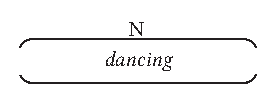
\includegraphics{figures/GrafikActivity.eps}
\end{center}
\caption{Phasal structure of activity}
\label{FigureActivity}
\end{figure}
The traditional label \textit{activity} has been adopted for reasons of familiarity. It is important to notice that in Nyakyusa this class of verbs not only encompasses actions performed by a volitional agent,\is{semantic roles} such as \textit{kama} `milk', \textit{keeta} `look', \textit{lɪma} `cultivate' or \textit{lya} `eat', but also dynamisms such as \textit{bala} `shine (of sun)', \textit{tima} `rain' and verbs traditionally subsumed under states, such as \textit{swiga} `wonder' and \textit{tiila} `fear, obey, respect'. All of these pattern together in their syntactic\is{syntax} and semantic behaviour. \citet[271f]{SeidelF2008} makes a similar observation for \ili{Yeyi} R41.  Semelfactives such as \textit{kema} \lq bark' or \textit{kosomola} \lq cough' may also be subsumed under the category of activities. These verbs normally give a series reading and otherwise pattern with activities in the relevant diagnostic criteria.
 
In the simple present, activity verbs denote an ongoing activity or process (\ref{exActivityPRS}), although they may also have a habitual/generic\is{aspect!habitual}\is{aspect!generic} or \isi{futurate} reading. Similarly, the periphrastic progressive gives an ongoing reading (\ref{exActivityPROG}).

\begin{exe}
\ex \label{exActivityPRS}
\begin{xlist}
\ex \gll i-kʊ-mog-a\\
 1-\textsc{prs}-dance-\textsc{fv}\\
\glt `S/he is dancing.'
\ex \gll ɪɪ-fula jɪ-kʊ-tim-a\\
\textsc{aug}-rain(9) 9-\textsc{prs}-rain-\textsc{fv}\\
\glt `It is raining.'
\ex \gll ɪ-m-bwa jɪ-kʊ-kem-a\\
\textsc{aug}-9-dog 9-\textsc{prs}-bark-\textsc{fv}\\
\glt `A/the dog is barking.'
\end{xlist}

\ex \label{exActivityPROG}
\begin{xlist}
\ex \gll a-lɪ pa-kʊ-mog-a\\
1-\textsc{cop} 16-15-dance-\textsc{fv}\\
\glt `S/he is dancing.'
\ex \gll ɪɪ-fula jɪ-lɪ pa-kʊ-tim-a\\
\textsc{aug}-rain(9) 9-\textsc{cop} 16-15-rain-\textsc{fv}\\
\glt \lq It is raining.'
\ex \gll ɪ-m-bwa jɪ-lɪ pa-kʊ-kem-a\\
\textsc{aug}-9-dog 9-\textsc{cop} 16-15-bark-\textsc{fv}\\
\glt `A/the dog is barking.'
\end{xlist}
\end{exe}

The simple present as the complement of the persistive aspect auxiliary has a reading of a continuing process and can also have a persistent habitual/generic\is{aspect!habitual}\is{aspect!generic} reading:
\begin{exe}
\ex \label{exActivityPersPRS}
\begin{xlist}
\ex \gll a-kaalɪ i-kʊ-mog-a\\
1-\textsc{pers} 1-\textsc{prs}-dance-\textsc{fv}\\
\glt 1. \lq S/he is still dancing.' \\ 2. \lq S/he still dances.'

\ex \gll ɪɪ-fula jɪ-kaalɪ jɪ-kʊ-tim-a\\
\textsc{aug}-rain(9) 9-\textsc{pers} 9-\textsc{prs}-rain-\textsc{fv}\\
\glt 1. \lq It is still raining.' \\ 2. \lq It still rains.'
\ex \gll ɪ-m-bwa jɪ-kaalɪ jɪ-kʊ-kem-a\\
\textsc{aug}-9-dog 9-\textsc{pers} 9-\textsc{prs}-bark-\textsc{fv}\\
\glt 1. \lq A/the dog is still barking.' \\ 2. \lq A/the dog still barks.'
\end{xlist}
\end{exe}

In the present perfective, activity verbs denote a past eventuality (\ref{exActivityPFV}). Note that this also holds for state-like verbs such as \textit{tiila} \lq  fear' (\ref{exTiilaPfv}). As the class of activities does not encode a resultant state, perfective aspect is not licensed in the complement of the persistive (\ref{exActivityNotPersPFV}).

\begin{exe}
\begin{multicols}{2}
\ex \label{exActivityPFV}
\begin{xlist}
\ex \gll a-mog-ile\\
1-dance-\textsc{pfv}\\
\glt `S/he has danced.'
\ex \gll ɪɪ-fula jɪ-tim-ile\\
\textsc{aug}-rain(9) 9-rain-\textsc{pfv}\\
\glt `It has rained.'
\ex \gll ɪ-m-bwa jɪ-kem-ile\\
\textsc{aug}-9-dog 9-bark-\textsc{pfv}\\
\glt `A/the dog has barked.'
\ex \label{exTiilaPfv}\gll a-kʊ-tiil-ile\\
1-\textsc{2sg}-fear-\textsc{pfv}\\
\glt \lq S/he has feared you.'
\end{xlist}
\end{multicols}
\clearpage
\ex\label{exActivityNotPersPFV} \begin{xlist}
\ex[*]{\gll a-kaalɪ a-mog-ile\\ 
1-\textsc{pers} 1-dance-\textsc{pfv}\\}
\ex[*]{\gll ɪɪ-fula jɪ-kaalɪ jɪ-tim-ile\\
\textsc{aug}-rain(9) 9-\textsc{pers} 9-rain-\textsc{pfv}\\}
\ex[*]{\gll ɪ-m-bwa jɪ-kaalɪ jɪ-kem-ile\\
\textsc{aug}-9-dog 9-\textsc{pers} 9-bark-\textsc{pfv}\\}
\ex[*]{\gll a-kaalɪ a-kʊ-tiil-ile\\
1-\textsc{pers} 1-\textsc{2sg}-fear-\textsc{pfv}\\}
\end{xlist}
\end{exe}

As activity verbs do not encode an inherent endpoint, they are not directly compatible with the time-span verb phrase \lq take X time'. Two repair readings are available, however, and most activity verbs allow for at least one of the two. The first is a conative reading denoting the time that elapses before the beginning of the lexical act (see \citealt[57]{DowtyD1979} for a similar observation for English).\il{English} The second repair reading is that of a quasi-accomplishment; see p. \pageref{QuasiAccomplishment} below for discussion.

\begin{exe}
\ex\label{exActivityTakeXTime}
\begin{xlist}
\ex \gll eeg-ile a-ka-balɪlo a-ka-tali ʊ-kʊ-mog-a\\
1.take-\textsc{pfv} \textsc{aug}-12-time \textsc{aug}-12-long \textsc{aug}-15-dance-\textsc{fv}\\
\glt 1. \lq S/he took a long time to (begin to) dance.'\\
2. \lq S/he took a long time to finish dancing (i.e. at a social event).'

\ex \gll eeg-ile a-ka-balɪlo a-ka-tali ʊ-kʊ-ly-a\\
1.take-\textsc{pfv} \textsc{aug}-12-time \textsc{aug}-12-long \textsc{aug}-15-eat-\textsc{fv}\\
\glt 1. \lq  S/he took a long time to begin to eat.'\\
2. \lq  S/he took a long time to eat (i.e. finish the meal).' 

\ex \gll eeg-ile a-ka-balɪlo a-ka-pimba ʊ-kʊ-kosomol-a\\
1.take-\textsc{pfv} \textsc{aug}-12-time \textsc{aug}-12-short \textsc{aug}-15-cough-\textsc{fv}\\
\glt \lq S/he took a short time to finish coughing (i.e. overcome illness).'
\end{xlist}
\end{exe}

The auxiliary \textit{anda} `begin, start' refers to the beginning of the activity (\ref{exActivityAnda1}, \ref{exActivityAnda2}), or in the case of semelfactives the beginning of the series (\ref{exActivitySemelfactiveAnda}).

\begin{exe}
\ex \begin{xlist}
\ex \label{exActivityAnda1}\gll and-ile ʊ-kʊ-mog-a\\
1.begin-\textsc{pfv} \textsc{aug}-15-dance-\textsc{fv}\\
\glt `S/he has started to dance.' 
\ex \label{exActivityAnda2} \gll ɪɪ-fula j-and-ile ʊ-kʊ-tim-a\\
\textsc{aug}-rain(9) 9-begin-\textsc{pfv} \textsc{aug}-15-rain-\textsc{fv}\\
\glt `It has started to rain.'
\ex \label{exActivitySemelfactiveAnda}\gll ɪ-m-bwa j-and-ile ʊ-kʊ-kem-a\\
\textsc{aug}-9-dog 9-begin-\textsc{pfv} \textsc{aug}-15-bark-\textsc{fv}\\
\glt `A/the dog has started to bark.'
\end{xlist}
\end{exe}

\label{QuasiAccomplishment} The terminative auxiliary \textit{mala} can be used with some but not all activity verbs. This is apparently dependent on two factors. First, a \lq\lq quasi-accomplishment sense'' \citep[176]{BinnickR1991} needs to be available. Binnick, on the basis of \citet[61]{DowtyD1979}, observes that this is the case when one speaks about an activity that forms part of or constitutes a specific task or habit. The second requirement is not one of phasal structure, but of thematic relations, namely that the subject be an agent or force.\is{semantic roles} The latter is in agreement with the findings on simple and transitional accomplishments (\sectref{VerbalClassSimpleAccomplishment}, \ref{VerbalClassTransitionalAccomplishment}, respectively); see also \citet[135]{FreedA1979} on \ili{English} \textit{finish}. Thus compare (\ref{exActivityMalaOK1}, \ref{exActivityMalaOK2}) to (\ref{exActivityMalaBad1}, \ref{exActivityMalaBad2}).
\begin{exe}
\ex\begin{xlist}
\ex[]{\label{exActivityMalaOK1}\gll a-mal-ile ʊ-kʊ-mog-a\\
1-finish-\textsc{pfv} \textsc{aug}-15-dance-\textsc{fv}\\
\glt \lq S/he has finished dancing.'}
\ex[]{\label{exActivityMalaOK2}\gll ɪ-m-bwa jɪ-mal-ile ʊ-kʊ-kem-a\\
\textsc{aug}-9-dog 9-finish-\textsc{pfv} \textsc{aug}-15-bark-\textsc{fv}\\
\glt \lq The dog has finished barking.'}
\ex[*]{\label{exActivityMalaBad1}\gll ɪɪ-fula jɪ-mal-ile ʊ-kʊ-tim-a\\
\textsc{aug}-rain(9) 9-finish-\textsc{pfv} \textsc{aug}-15-rain-\textsc{fv}\\
\glt (intended: \lq The rain has finished.')}
\ex[*]{\label{exActivityMalaBad2}\gll a-mal-ile ʊ-kʊ-n-diil-a\\
1-finish-\textsc{pfv} \textsc{aug}-15-\textsc{1sg}-fear-\textsc{fv}\\
\glt (intended: \lq S/he is done fearing me.')}
\end{xlist}
\end{exe}

Lastly, the egressive auxiliary \textit{leka} denotes a cessation or interruption:
\begin{exe}
\ex
\begin{xlist}
\ex \gll a-lek-ile ʊ-kʊ-mog-a\\
1-cease-\textsc{pfv} \textsc{aug}-15-dance-\textsc{pfv}\\
\glt \lq S/he has stopped dancing.'
\ex \gll ɪɪ-fula jɪ-lek-ile ʊ-kʊ-tim-a\\
\textsc{aug}-rain(9) 9-cease-\textsc{pfv} \textsc{aug}-15-rain-\textsc{pfv}\\
\glt \lq It has stopped raining.'
\ex \gll ɪ-m-bwa jɪ-lek-ile ʊ-kʊ-kem-a\\
\textsc{aug}-9-dog 9-cease-\textsc{pfv} \textsc{aug}-15-bark-\textsc{fv}\\
\glt \lq A/the dog has stopped barking.'
\end{xlist}
\end{exe}

\subsection{Simple accomplishments}\label{VerbalClassSimpleAccomplishment}
Simple accomplishments encode an activity that is delimited by an endpoint. That is, they correspond to \citeauthor{VendlerZ1957}'s (\citeyear{VendlerZ1957}) \textit{accomplishments}. Following \citet{BotneR2008}, the qualification \textit{simple} has been adopted to distinguish them from their transitional counterpart (\sectref{VerbalClassTransitionalAccomplishment}). The phasal structure of simple accomplishments can be schematized as in \figref{FigureSimpleAccomplishment} for \textit{pona} \lq recover'. Other lexical verbs of this class are \textit{bɪfwa} \lq ripen', \textit{lembʊka} \lq wake up, get up' and \textit{talalɪla} \lq cool (intr.)'. Accomplishments can also be derived from activities, e.g. by means of a quantized primary object, as in \textit{lya ɪngʊkʊ joosa} \lq eat a whole chicken' or \textit{kama ɪɪng'ombe syosa} \lq milk all cows' (see \citealt{VerkuylH1972}; \citealt{DowtyD1979}). The derivation of accomplishments through other means, such as measure (\lq walk a mile') or goal noun phrases (\lq walk to the park') is open to further research. Note that in Nyakyusa, objects, once they have been introduced into discourse, are often understood from context without repetition or cross-referencing. Lastly, it should be noted that not all simple accomplishments constitute actions performed by a volitional agent.\is{semantic roles} The same is true for activity verbs.

\begin{figure}[h]
\begin{center}
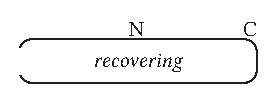
\includegraphics{figures/GrafikSimpleAccomplishment.eps}
\end{center}
\caption{Phasal structure of simple accomplishment}
\label{FigureSimpleAccomplishment}
\end{figure}
Like activity verbs and transitional accomplishments, simple accomplishments denote an ongoing process in the simple present (\ref{exSimpleAccomplishmentPRS}), although they may also have a futurate and habitual or generic reading.\is{aspect!habitual}\is{aspect!generic} In the same vein, the periphrastic progressive refers to the process of change (\ref{exSimpleAccomplishmentPROG}).

\begin{exe}
\ex \label{exSimpleAccomplishmentPRS}
\begin{xlist}
\ex \gll ʊ-m̩-bine i-kʊ-pon-a\\
\textsc{aug}-1-ill 1-\textsc{prs}-recover-\textsc{fv}\\
\glt \lq A/the sick person is recovering.'

\ex \gll i-kʊ-lembʊk-a\\
1-\textsc{prs}-awake-\textsc{fv}\\
\glt \lq S/he is waking up.'

\ex \gll i-kʊ-ly-a ɪ-n-gʊkʊ j-oosa\\
1-\textsc{prs}-eat-\textsc{fv} \textsc{aug}-9-chicken 9-all\\
\glt \lq S/he is eating a whole chicken.'
\end{xlist}
\ex \label{exSimpleAccomplishmentPROG}
\begin{xlist}
\ex \gll ʊ-m̩-bine a-lɪ pa-kʊ-pon-a\\
\textsc{aug}-1-ill 1-\textsc{cop} 16-15-recover-\textsc{fv}\\
\glt \lq A/the sick person is recovering.'

\ex \gll a-lɪ pa-kʊ-lembʊk-a\\
1-\textsc{cop} 16-15-awake-\textsc{fv}\\
\glt \lq S/he is waking up.'

\ex \gll a-lɪ pa-kʊ-ly-a ɪ-n-gʊkʊ j-oosa\\
1-\textsc{cop} 16-15-eat-\textsc{fv} \textsc{aug}-9-chicken 9-all\\
\glt \lq S/he is eating a whole chicken.'
\end{xlist}
\end{exe}

As expected, the combination of persistive aspect and the simple present denotes the continuation of the process and further allows for a persistent habitual/generic reading:\is{aspect!habitual}\is{aspect!generic}

\begin{exe}
\ex
\begin{xlist}
\ex \gll ʊ-m̩-bine a-kaalɪ i-kʊ-pon-a\\
\textsc{aug}-1-ill 1-\textsc{pers} 1-\textsc{prs}-recover-\textsc{fv}\\
\glt 1. \lq  A/the sick person is still recovering.'\\ 2. \lq  A/the sick person still recovers (frequently).'

\ex \gll a-kaalɪ i-kʊ-lembʊk-a\\
1-\textsc{pers} 1-\textsc{prs}-awake-\textsc{fv}\\
\glt 1. \lq S/he is still waking up.'\\ 2. \lq S/he still wakes up.'

\ex \gll a-kaalɪ i-kʊ-ly-a ɪ-n-gʊkʊ j-oosa\\
1-\textsc{pers} 1-\textsc{prs}-eat-\textsc{fv} \textsc{aug}-9-chicken 9-all\\
\glt 1. \lq S/he is still [occupied with] eating a whole chicken.'\\
2. \lq S/he still eats whole chickens.'
\end{xlist}
\end{exe}

In the present perfective, simple accomplishments denote that the eventuality has passed (\ref{exSimpleAccomplishmentPFV}). As they do not encode a resultant state, perfective aspect is not licensed in the complement of the persistive aspect auxiliary (\ref{exSimpleAccomplishmentNoPERSPFV}).

\begin{exe}
%keine multicols weil akaali aliile ... zu lang
\ex\label{exSimpleAccomplishmentPFV}
\begin{xlist}
\ex[]{ \gll ʊ-m̩-bine a-pon-ile\\
\textsc{aug}-1-ill 1-recover-\textsc{pfv}\\
\glt \lq A/the sick person has recovered.'}

\ex[]{ \gll a-lembwike\\
1-awake.\textsc{pfv}\\
\glt \lq S/he has woken up.'}

\ex[]{ \gll a-l-iile ɪ-n-gʊkʊ j-oosa\\
1-eat-\textsc{pfv} \textsc{aug}-9-chicken 9-all\\
\glt \lq S/he has eaten a whole chicken.'}
\end{xlist}
\ex\label{exSimpleAccomplishmentNoPERSPFV} \begin{xlist}
\ex[*]{\gll a-kaalɪ a-pon-ile\\
1-\textsc{pers} 1-recover-\textsc{pfv}\\
\glt (intended: \lq S/he is still healed.')}
\ex[*]{\gll a-kaalɪ a-lembwike\\
1-\textsc{pers} 1-awake.\textsc{pfv}\\
\glt (intended: \lq S/he is still awake.')}
\ex[*]{\gll a-kaalɪ a-l-iile ɪ-n-gʊkʊ j-oosa\\
1-\textsc{pers} 1-eat-\textsc{pfv} \textsc{aug}-9-chicken 9-all\\
\glt (intended: \lq S/he is still full from eating a whole chicken.')}
\end{xlist}
\end{exe}%keine multicols, weil zu lang

With simple accomplishments, the time-span verb phrase \lq take X time' unambiguously refers to the time that elapses before the culmination of the process.

\begin{exe}
\ex
\begin{xlist}
\ex \gll ʊ-m̩-bine eeg-ile a-ka-balɪlo a-ka-tali ʊ-kʊ-pon-a\\
\textsc{aug}-1-ill 1.take-\textsc{pfv} \textsc{aug}-12-time \textsc{aug}-12-long \textsc{aug}-15-recover-\textsc{fv}\\
\glt \lq A/the sick person has taken a long time to recover.'

\ex \gll eeg-ile ɪɪ-sala j-oosa ʊ-kʊ-lembʊk-a\\
1.take-\textsc{pfv} \textsc{aug}-hour(9) 9-all \textsc{aug}-15-awake-\textsc{fv}\\
\glt \lq S/he has taken a whole hour to wake up.'

\ex \gll eeg-ile a-ka-balɪlo a-ka-pimba ʊ-kʊ-ly-a ɪ-n-gʊkʊ j-oosa\\
1.take-\textsc{pfv} \textsc{aug}-12-time \textsc{aug}-12-short \textsc{aug}-15-eat-\textsc{fv} \textsc{aug}-9-chicken 9-all\\
\glt \lq S/he has taken a short time to eat a whole chicken.'
\end{xlist}
\end{exe}

The ingressive auxiliary \textit{anda} \lq start, begin' refers to the beginning of the process:
\begin{exe}
\ex\begin{xlist}
\ex \gll ʊ-m̩-bine and-ile ʊ-kʊ-pon-a\\
\textsc{aug}-1-ill 1.begin-\textsc{pfv} \textsc{aug}-15-recover-\textsc{fv}\\
\glt \lq A/the sick person has begun to recover.'

\ex \gll and-ile ʊ-kʊ-lembʊk-a\\
1.begin-\textsc{pfv} \textsc{aug}-15-awake-\textsc{fv}\\
\glt \lq S/he has begun to wake up.'

\ex \gll and-ile ʊ-kʊ-ly-a ɪ-n-gʊkʊ j-oosa\\
1.begin-\textsc{pfv} \textsc{aug}-15-eat-\textsc{fv} \textsc{aug}-9-chicken 9-all\\
\glt \lq S/he has started to eat a whole chicken.'
\end{xlist}
\end{exe}
The terminative auxiliary \textit{mala} is compatible with some, but not all, accomplishments and denotes that the process has been completed. As with activity verbs in their quasi-accomplishment reading, and as will be seen for transitional accomplishments (\sectref{VerbalClassTransitionalAccomplishment}), \textit{mala} requires a subject with the semantic role of agent or force:\is{semantic roles}

\begin{exe}
\ex\begin{xlist}
\ex[]{\label{exSimpleAccomplishmentMalaOK1}\gll a-mal-ile ʊ-kʊ-lembʊk-a\\
1-finish-\textsc{pfv} \textsc{aug}-15-awake-\textsc{fv}\\
\glt \lq S/he has finished getting up.'}
\ex[]{\label{exSimpleAccomplishmentMalaOK2}\gll a-mal-ile ʊ-kʊ-ly-a ɪ-n-gʊkʊ j-oosa\\
1-finish-\textsc{pfv} \textsc{aug}-15-eat-\textsc{fv} \textsc{aug}-9-chicken 9-all\\
\glt \lq S/he has finished eating a whole chicken.'}
\ex[*]{\label{exSimpleAccomplishmentMalaBad1}\gll ʊ-m̩-bine a-mal-ile ʊ-kʊ-pon-a\\
\textsc{aug}-1-ill 1-finish-\textsc{pfv} \textsc{aug}-15-recover-\textsc{fv}\\
\glt (intended: \lq A/the sick person has accomplished recovery.')}
\ex[*]{\label{exSimpleAccomplishmentMalaBad2}\gll a-ma-tooki ga-mal-ile ʊ-kʊ-bɪfw-a\\
\textsc{aug}-6-banana 6-finish-\textsc{pfv} \textsc{aug}-15-ripen-\textsc{fv}\\
\glt (intended: \lq The bananas have become completely ripe.')}
\end{xlist}
\end{exe}

Lastly, \textit{leka} \lq cease, stop' denotes a cessation or interruption of the process:
\begin{exe}
\ex\begin{xlist}
\ex \gll ʊ-m̩-bine a-lek-ile ʊ-kʊ-pon-a\\
\textsc{aug}-1-ill 1-cease-\textsc{pfv} \textsc{aug}-15-recover-\textsc{fv}\\
\glt \lq A/the sick person has ceased to recover.'

\ex \gll a-lek-ile ʊ-kʊ-lembʊk-a\\
1-cease-\textsc{pfv} \textsc{aug}-15-awake-\textsc{fv}\\
\glt \lq S/he has ceased to wake up (viz. fallen asleep again).'

\ex \gll a-lek-ile ʊ-kʊ-ly-a ɪ-n-gʊkʊ j-oosa\\
1-cease-\textsc{pfv} \textsc{aug}-15-eat-\textsc{fv} \textsc{aug}-9-chicken 9-all\\
\glt \lq S/he has ceased eating a whole chicken.'
\end{xlist}
\end{exe} 

\subsection{Transitional accomplishments}\label{VerbalClassTransitionalAccomplishment}
\is{inchoative verbs|(}Transitional accomplishments encode a process that leads to a new state. They thus share characteristics of activity verbs and simple accomplishments on the one hand and of inchoative achievement verbs (\sectref{VerbalClassTransitionalAchievement}, \ref{VerbalClassResultativeAchievement}) on the other. Note that a distinction between transitional achievements and transitional accomplishments has so far only been observed for neighbouring \ili{Ndali} \citep{BotneR2008}. Its importance for a theory of Aristotelian aspect is highlighted in \citet{PersohnB2017b}. More systematic research on Aristotelian aspect in other Bantu languages might bring to light similar distinctions.

The phasal structure of transitional accomplishments can be schematized as in \figref{FigureTransitionalAccomplishment} for \textit{gaala} \lq get drunk, be drunk'. Other verbs of this class include \textit{fwala} `dress, wear', \textit{isʊla} \lq swell, be full', and \textit{onangɪka} \lq be(come) spoiled'. As becomes most clear with the last two verbs, and as is the case with activity verbs and simple accomplishments, the lexicalized process need not be dependent on a volitional agent.\is{semantic roles}

\begin{figure}[h]
\begin{center}

\includegraphics{figures/GrafikTransitionalAccomplishment.eps}
\end{center}
\caption{Phasal structure of transitional accomplishment}
\label{FigureTransitionalAccomplishment}
\end{figure}

Like activity verbs and simple accomplishments, transitional accomplishments denote an ongoing process in the simple present (\ref{exTransitionalAccomplishmentPRS}), as well as a possible futurate or habitual/generic reading.\is{aspect!habitual}\is{aspect!generic} In the same vein, the periphrastic progressive refers to the process of change (\ref{exTransitionalAccomplishmentPROG}).
\begin{exe}
\ex \label{exTransitionalAccomplishmentPRS}
\begin{xlist}
\ex\gll i-kʊ-gaal-a\\
1-\textsc{prs}-be(come)\_drunk-\textsc{fv}\\
\glt `S/he is getting drunk.'
\ex\gll i-kʊ-fwal-a \textup{(}ii-koti\textup{)}\\
1-\textsc{prs}-dress/wear-\textsc{fv} (5-coat<SWA)\\
\glt `S/he is dressing (putting on a/the coat).'
\end{xlist}
\ex \label{exTransitionalAccomplishmentPROG}
\begin{xlist}
\ex\gll a-lɪ pa-kʊ-gaal-a\\
1-\textsc{cop} 16-15-be(come)\_drunk-\textsc{fv}\\
\glt `S/he is getting drunk.'
\ex\gll a-lɪ pa-kʊ-fwal-a \textup{(}ii-koti\textup{)}\\
1-\textsc{cop} 16-15-dress/wear-\textsc{fv} (5-coat)\\
\glt `S/he is dressing (putting on a/the coat).'
\end{xlist}
\end{exe}

\largerpage
Also like activities and simple accomplishments, but unlike transitional achievements, the simple present as the complement of the persistive aspect auxiliary denotes the continuation of the pre-culmination process:
\begin{exe}
\ex\label{exTransitionalAccomplishmentPERSPRS}
\begin{xlist}
\ex\gll a-kaalɪ i-kʊ-gaal-a\\
1-\textsc{pers} 1-\textsc{prs}-be(come)\_drunk-\textsc{fv}\\
\glt 1. \lq S/he still gets drunk (regularly).'\\
2. \lq S/he is still getting drunk.'
\ex\gll a-kaalɪ i-kʊ-fwal-a \textup{(}ii-koti\textup{)}\\
1-\textsc{pers} 1-\textsc{prs}-dress/wear-\textsc{fv} (5-coat)\\
\glt 1. \lq S/he still dresses (puts on a/the coat).'\\
2. \lq S/he is still dressing (putting on a/the coat).'
\end{xlist}
\end{exe}

As with all inchoative verbs, but unlike activities and simple accomplishments, the perfective of transitional accomplishments is licensed as the complement of the persistive aspect auxiliary (\ref{exTransitionalAccomplishmentPERSPFV}), a combination that denotes a persistent resultant state.
\begin{exe}
\ex \label{exTransitionalAccomplishmentPERSPFV}\begin{xlist}
\ex\gll a-kaalɪ a-gaal-ile\\
1-\textsc{pers} 1-be(come)\_drunk-\textsc{pfv}\\
\glt `S/he is still drunk.'
\ex \gll a-kaalɪ a-fweele \textup{(}ii-koti\textup{)}\\
1-\textsc{pers} 1-dress/wear.\textsc{pfv} (5-coat)\\
\glt `S/he is still dressed (with a/the coat).'
\end{xlist}
\end{exe}

The time-span phrase \lq take X time', as with simple accomplishments, refers to the time elapsing before the culmination:
\begin{exe}
\ex \begin{xlist}
\ex \gll eeg-ile a-ka-balɪlo a-ka-tali ʊ-kʊ-gaal-a\\
1.take-\textsc{pfv} \textsc{aug}-12-time \textsc{aug}-12-long \textsc{aug}-15-be(come)\_drunk-\textsc{fv}\\
\glt \lq S/he took a long time to get drunk.'
\ex \gll eeg-ile a-ka-balɪlo a-ka-tali ʊ-kʊ-fwal-a \textup{(}ii-koti\textup{)}\\
1.take-\textsc{pfv} \textsc{aug}-12-time \textsc{aug}-12-long \textsc{aug}-15-dress/wear-\textsc{fv} (5-coat)\\
\glt \lq S/he took a long time to dress (put on a/the coat).'
\end{xlist}
\end{exe}

The auxiliary \textit{anda} \lq begin, start' in the single event reading denotes the beginning of the process of change:
\begin{exe}
\ex\begin{xlist}
\ex \gll and-ile ʊ-kʊ-gaal-a\\
1.begin-\textsc{pfv} \textsc{aug}-15-be(come)\_drunk-\textsc{fv}\\
\glt \lq S/he has begun to get drunk.'
\ex \gll and-ile ʊ-kʊ-fwal-a \textup{(}ii-koti\textup{)}\\
1.begin-\textsc{pfv} \textsc{aug}-15-dress/wear-\textsc{fv} (5-coat)\\
\glt \lq S/he has started to dress (to put on a/the coat).'
\end{xlist}
\end{exe}

The auxiliary \textit{mala} `finish' with transitional accomplishments can have a single event reading, in which case it refers to the culmination of the process. This behaviour is shared with activities and simple accomplishments, but not with transitional achievements. To be compatible with \textit{mala} requires the subject to have the semantic role of agent or force,\is{semantic roles} as in (\ref{exTransitionalAccomplishmentMalaOK1}, \ref{exTransitionalAccomplishmentMalaOK2}) but not (\ref{exTransitionalAccomplishmentMalaBad}).
\begin{exe}
\ex\begin{xlist}
\ex[]{\label{exTransitionalAccomplishmentMalaOK1}\gll a-mal-ile ʊ-kʊ-gaal-a\\
1-finish-\textsc{pfv} \textsc{aug}-15-be(come)\_drunk-\textsc{fv}\\
\glt \lq S/he has finished getting drunk (purposefully).'}
\ex[]{\label{exTransitionalAccomplishmentMalaOK2}\gll a-mal-ile ʊ-kʊ-fwal-a \textup{(}ii-koti\textup{)}\\
1-finish-\textsc{pfv} \textsc{aug}-15-dress/wear-\textsc{fv} (5-coat)\\
\glt \lq S/he has finished dressing (putting on a/the coat).'}
\ex[*]{\label{exTransitionalAccomplishmentMalaBad}\gll ii-galɪ lɪ-mal-ile ʊ-k-oonangɪk-a\\
5-car 5-finish-\textsc{pfv} \textsc{aug}-15-be(come)\_spoiled-\textsc{fv}\\
\glt (intended: \lq A/the car has broken down completely.')}
\end{xlist}
\end{exe}

Lastly, \textit{leka} \lq cease, stop' in a single event reading refers to a cessation or interruption of the process:
\begin{exe}
\ex \begin{xlist}
\ex \gll a-lek-ile ʊ-kʊ-gaal-a\\
1-cease-\textsc{pfv} \textsc{aug}-15-be(come)\_drunk-\textsc{fv}\\
\glt `S/he has ceased to get drunk (e.g. stopped drinking).'
\ex \gll a-lek-ile ʊ-kʊ-fwal-a \textup{(}ii-koti\textup{)}\\
1-cease-\textsc{pfv} \textsc{aug}-15-dress/wear-\textsc{fv} (5-coat)\\
\glt `S/he has stopped dressing (putting on a/the coat).'
\end{xlist}
\end{exe}
\is{inchoative verbs|)}
\subsection{Transitional achievements}\label{VerbalClassTransitionalAchievement}
\is{inchoative verbs|(}
Transitional achievements encode a change-of-state as well a pre-culmination state and a resultant state. Their phasal structure can thus be schematized as in \figref{FigureTransitionalAchievement} for \textit{kalala} `be(come) angry'. This class of verbs makes up the vast majority of achievements in the sample. Other examples include \textit{fugama} \lq kneel', \textit{fwa} `die', \textit{gwa paasi} \lq fall down', \textit{katala} `be(come) tired', \textit{kola} \lq grasp, hold' and \textit{nyala} \lq be(come) dirty'.

\begin{figure}[h]
\begin{center}

\includegraphics{figures/GrafikTransitionalAchievement.eps}
\caption{Phasal structure of transitional achievement}
\label{FigureTransitionalAchievement}
\end{center}
\end{figure}

In the simple present, transitional achievements have a coming-to-be reading (\ref{exTransitionalAchievementPRS}), as well as a habitual/generic\is{aspect!habitual}\is{aspect!generic} and a \isi{futurate} one. Likewise, the periphrastic progressive refers to the coming-to-be. Typically this is understood as being close to a change-of-state (\ref{exTransitionalAchievementPROG}).
\begin{exe}
\begin{multicols}{2}
\ex\label{exTransitionalAchievementPRS} \begin{xlist}
\ex \gll i-kʊ-kalal-a\\
1-\textsc{prs}-be(come)\_angry-\textsc{fv} \phantom{16-15}\\
\glt `S/he is becoming angry.'
\ex \gll i-kʊ-fw-a\\
1-\textsc{prs}-die-\textsc{fv}\\
\glt `S/he is dying.'
\end{xlist}
\columnbreak
\ex\label{exTransitionalAchievementPROG} \begin{xlist}
\ex \gll a-lɪ pa-kʊ-kalal-a\\
1-\textsc{cop} 16-15-be(come)\_angry-\textsc{fv}\\
\glt `S/he is about to be angry.'
\ex \gll a-lɪ pa-kʊ-fw-a\\
1-\textsc{cop} 16-15-die-\textsc{fv}\\
\glt `S/he is about to die.'
\end{xlist}
\end{multicols} 
\end{exe}%hier muss vllt getrickst werden mit \vspace*{\fill} nach jeweils dem ersten bsp o.ae.

Some, but not all, transitional achievements can be used with the simple present as the complement of the persistive aspect auxiliary (\ref{exTransitionalAchievementPERSPRS}). In this case, what is referred to is the continuation of the resultant state. This behaviour is shared with resultative achievements (\sectref{VerbalClassResultativeAchievement}) but not with transitional accomplishments (\sectref{VerbalClassTransitionalAccomplishment}). However, those language assistants that accepted these readings were either hesitant at first or considered these readings to be less natural than the use of the persistive plus perfective aspect, which makes this look like a clear case of coercion; see \citet{MichaelisL2004} for a theory of coercion.

\begin{exe}
\ex \label{exTransitionalAchievementPERSPRS}\begin{xlist}
\ex[]{\gll a-kaalɪ i-kʊ-fugam-a\\
1-\textsc{pers} 1-\textsc{prs}-kneel-\textsc{fv}\\
\glt 1. \lq S/he still kneels.'\\
2. \lq  S/he is still kneeling.'}
\ex[*]{\gll a-kaalɪ i-kʊ-fw-a\\
1-\textsc{pers} 1-\textsc{prs}-die-\textsc{fv}\\
\glt (intended: \lq S/he is still being dead.')}
\end{xlist}
\end{exe}

As with all inchoative verbs, the perfective form of transitional achievements is licensed as the complement of the persistive aspect auxiliary (\ref{exTransitionalAchievementPersPFV}).
\begin{exe}
\ex \label{exTransitionalAchievementPersPFV}\begin{xlist}
\ex\gll a-kaalɪ a-kaleele\\
1-\textsc{pers} 1-be(come)\_angry.\textsc{pfv}\\
\glt `S/he is still angry.'
\ex \gll ii-lʊʊka lɪ-kaalɪ lɪ-fw-ile\\
5-store 5-\textsc{pers} 5-die-\textsc{pfv}\\
\glt `The store is still dead (viz. closed).'
\end{xlist}
\end{exe}

The ingressive auxiliary \textit{anda} `begin, start' refers to the beginning of the development:
\begin{exe}
\ex \begin{xlist}
\ex \gll and-ile ʊ-kʊ-kalal-a\\
1.begin-\textsc{pfv} \textsc{aug}-15-be(come)\_angry-\textsc{fv}\\
\glt `S/he has started to become angry.'
\ex \gll and-ile ʊ-kʊ-fw-a\\
1.begin-\textsc{pfv} \textsc{aug}-15-die-\textsc{fv}\\
\glt `S/he has started to die.'
\end{xlist}
\end{exe}
Some transitional achievements are compatible with \textit{mala} \lq finish', in which case the reference is to the eventuality as a whole. As observed in \sectref{VerbalClassActivities}--\ref{VerbalClassTransitionalAccomplishment}, this requires the subject to have the semantic role\is{semantic roles} of agent or force, or to be construable as such. Thus compare (\ref{exTransitionalAchievementMala1}, \ref{exTransitionalAchievementMala2}) to (\ref{exTransitionalAchievementMala3}, \ref{exTransitionalAchievementMala4}):

\begin{exe}
\ex
\begin{xlist}
\ex[]{\label{exTransitionalAchievementMala1}\gll a-mal-ile ʊ-kʊ-kol-a ii-bwe\\
1-finish-\textsc{pfv} \textsc{aug}-15-grasp/hold-\textsc{fv} 5-stone\\
\glt \lq S/he has finished holding a/the stone.'
}
\ex[]{\label{exTransitionalAchievementMala2}\gll a-mal-ile ʊ-kʊ-fugam-a\\
1-finish-\textsc{pfv} \textsc{aug}-15-kneel-\textsc{fv}\\
\glt \lq S/he has finished kneeling.'}

\ex[?]{\label{exTransitionalAchievementMala3}\gll a-mal-ile ʊ-kʊ-kalal-a\\
1-finish-\textsc{pfv} \textsc{aug}-15-be(come)\_angry-\textsc{fv}\\
\glt \lq S/he has finished being angry.'}

\ex[*]{\label{exTransitionalAchievementMala4}\gll ii-lʊʊka lɪ-mal-ile ʊ-kʊ-fw-a\\
5-store 5-finish-\textsc{pfv} \textsc{aug}-15-die-\textsc{fv}\\
\glt (intended: \lq The store is not closed anymore (i.e. has opened again).')}
\end{xlist}
\end{exe}

Likewise, a single event reading with the egressive auxiliary \textit{leka} is available for some, but not all, transitional achievements. In accordance with their meaningful focus on the resultant state, this denotes an interruption or cessation of the latter. It is not entirely clear what the determining semantic factors are. The following examples suggest that at least world knowledge comes into play:

\begin{exe}
\ex\begin{xlist}
\ex[]{\label{exTransAchievementLeka1}\gll a-lek-ile ʊ-kʊ-fugam-a\\
1-cease-\textsc{pfv} \textsc{aug}-15-kneel-\textsc{fv}\\
\glt \lq S/he has ceased to be kneeling.'}
\ex[]{\label{exTransAchievementLeka2}\gll a-lek-ile ʊ-kʊ-kalal-a\\
1-cease-\textsc{pfv} \textsc{aug}-15-be(come)\_angry-\textsc{fv}\\
\glt \lq S/he has ceased to be angry.'}
\ex[?]{\gll ɪɪ-nyumba jɪ-lek-ile ʊ-kʊ-nyala-a\\
\textsc{aug}-house(9) 9-cease-\textsc{pfv} \textsc{aug}-15-be(come)\_dirty-\textsc{fv}\\
\glt \lq A/the house has ceased to be dirty.'}
\ex[*]{\gll ii-lʊʊka ly-a-fw-ile looli lɪ-lek-ile ʊ-kʊ-fw-a\\
5-store 5-\textsc{pst}-die-\textsc{pfv} but 5-cease-\textsc{pfv} \textsc{aug}-15-die-\textsc{fv}\\
\glt (intended: \lq The store was closed but it is not closed anymore.')}
\end{xlist}
\end{exe}

The language assistants commented that examples such as (\ref{exTransAchievementLeka1}, \ref{exTransAchievementLeka2}) are acceptable but not very natural. A more common way to refer to a state, e.g. of anger, that has come to an end would be the following:

\begin{exe}
\ex 
\begin{xlist}
\gll a-a-kaleele, looli si-mal-iike\\
1-\textsc{pst}-be(come)\_angry.\textsc{pfv} now/but 10-finish-\textsc{neut.pfv}\\
\glt \lq S/he was angry, but now it is over.'
\end{xlist}
\end{exe}

Last, the time-span phrase \lq take X time' refers to the time elapsing before the change-of-state:

\begin{exe}
\ex  \gll eeg-ile a-ka-balɪlo a-ka-pimba fiijo ʊ-kʊ-kalal-a\\
1.take-\textsc{pfv} \textsc{aug}-12-time \textsc{aug}-12-short \textsc{intens} \textsc{aug}-15-be(come)\_angry-\textsc{fv}\\
\glt \lq S/he got angry in a very short time.'
\ex  \gll eeg-ile a-ka-balɪlo a-ka-tali ʊ-kʊ-fugam-a\\
1.take-\textsc{pfv} \textsc{aug}-12-time \textsc{aug}-12-short \textsc{aug}-15-kneel-\textsc{fv}\\
\glt \lq S/he took a lot of time to get on his/her knees.'
\end{exe}
\is{inchoative verbs|)}
\subsection{Resultative achievements}\label{VerbalClassResultativeAchievement}
\is{inchoative verbs|(}
Resultative achievements encode a change-of-state together with the resultant state. Their phasal structure can thus be schematized as in \figref{FigureResultativeAchievement} for \textit{hoboka} `be(come) happy'. Other examples are \textit{benga} \lq hate', \textit{gana} \lq like, love', \textit{gona ʊtʊlo} \lq sleep' and \textit{twala} \lq carry, bring'.

\begin{figure}[h]
\begin{center}
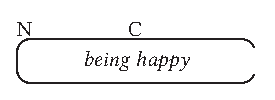
\includegraphics{figures/GrafikResultativeAchievement.eps}
\caption{Phasal structure of resultative achievement}
\label{FigureResultativeAchievement}
\end{center}
\end{figure}

In the simple present, resultative achievements have a \isi{futurate} reading as well as a habitual/generic one,\is{aspect!habitual}\is{aspect!generic} but no progressive reading (\ref{exResultiveAchievementPRS}).

\begin{exe}
\ex \label{exResultiveAchievementPRS} \begin{xlist}
\ex \gll i-kʊ-hobok-a\\
1-\textsc{prs}-be(come)\_happy-\textsc{fv}\\
\glt 1. `S/he will become happy.'\\2. `S/he becomes happy (e.g. on each particular occasion).' 

\ex \gll i-kʊ-m-beng-a\\
1-\textsc{prs}-\textsc{1sg}-hate-\textsc{fv}\\
\glt 1. \lq S/he will hate me.'\\
2. \lq S/he hates me (e.g. shows it every time we meet).'

\end{xlist}
\end{exe}

The periphrastic progressive construction with resultative achievements refers to the resultant state (\ref{exResultativeAchievementPROG}). This is unlike transitional achivements (\sectref{VerbalClassTransitionalAchievement}), which do encode an Onset state. 
\begin{exe}
\ex \label{exResultativeAchievementPROG}\begin{xlist}
\ex\gll a-lɪ pa-kʊ-hobok-a\\
1-\textsc{cop} 16-15-be(come)\_happy-\textsc{fv}\\
\glt `S/he is happy.'
\ex \gll a-lɪ pa-kʊ-m-beng-a\\
1-\textsc{cop} 16-15-\textsc{1sg}-hate-\textsc{fv}\\
\glt \lq S/he hates me (e.g. is acting hostile).'
\end{xlist}
\end{exe}

Some, but not all, resultative achievements can be coerced into a progressive reading with the simple present as the complement of the persistive aspect auxiliary (\ref{exResultativeAchievementPERSPRS}). As with transitional achievements, what is referred to in this case is the resultant state.

\begin{exe}
\ex \label{exResultativeAchievementPERSPRS}
\begin{xlist}
\ex\gll a-kaalɪ i-kʊ-hobok-a\\
1-\textsc{pers} 1-\textsc{prs}-be(come)\_happy-\textsc{fv}\\
\glt 1. \lq S/he still becomes happy.'\\
2. \lq  S/he is still being happy.'

\ex\gll a-kaalɪ i-kʊ-m-beng-a\\
1-\textsc{pers} 1-\textsc{prs}-\textsc{1sg}-hate-\textsc{fv}\\
\glt 1. \lq S/he still hates me (e.g. still shows it every time we meet).'\\
2. \lq  S/he is still hating me (e.g. acting hostile).'
\ex \gll a-kaalɪ i-kʊ-twal-a ɪ-kɪ-kapʊ\\
1-\textsc{pers} 1-\textsc{prs}-carry-\textsc{fv} \textsc{aug}-7-basket\\
\glt \lq S/he still carries a/the basket (regularly).'\\
not: \lq S/he is still carrying a/the basket.'
\end{xlist}
\end{exe}

As with all inchoative verbs, the common way to refer to the resultant state is with the use of the perfective aspect, which is licensed as the complement of the persistive aspect auxiliary (\ref{exResultativeAchievementPERSFV}), a combination that denotes the persistence of the resultant state.
\begin{exe}
\ex \label{exResultativeAchievementPERSFV}\begin{xlist}
\ex\gll a-kaalɪ a-hobwike\\
1-\textsc{pers} 1-be(come)\_happy.\textsc{pfv}\\
\glt `S/he is still happy.'

\ex \gll a-kaalɪ a-m-beng-ile\\
1-\textsc{pers} 1-\textsc{1sg}-hate-\textsc{pfv}\\
\glt \lq S/he still hates me.'
\end{xlist}
\end{exe}

The time-span phrase \lq take X time' refers to the time elapsing before the entry into the new state:

\begin{exe}
\ex \begin{xlist}
\ex \gll eeg-ile a-ka-balɪlo a-ka-tali ʊ-kʊ-hobok-a\\
1.take-\textsc{pfv} \textsc{aug}-12-time \textsc{aug}-12-long \textsc{aug}-15-be(come)\_happy-\textsc{fv}\\
\glt \lq S/he took a long time to become happy.'

\ex \gll eeg-ile a-ka-balɪlo a-ka-pimba ʊ-kʊ-m-beng-a\\
1.take-\textsc{pfv} \textsc{aug}-12-time \textsc{aug}-12-short \textsc{aug}-15-\textsc{1sg}-hate-\textsc{fv}\\
\glt \lq S/he came to hate me within a short time.'
\end{xlist}
\end{exe}

Related to the behaviour of resultative achievements with the simple present and periphrastic progressive, the auxiliary \textit{anda} `begin, start' in the single event reading refers to an initial subphase of the resultant state:
\begin{exe}
\ex \begin{xlist}
\ex \gll and-ile ʊ-kʊ-hobok-a\\
1.begin-\textsc{pfv} \textsc{aug}-15-be(come)\_happy-\textsc{fv}\\
\glt `S/he has begun to be happy.'
\ex\gll and-ile ʊ-kʊ-m-beng-a\\
1.begin-\textsc{pfv} \textsc{aug}-15-\textsc{1sg}-hate-\textsc{fv}\\
\glt \lq S/he has begun to hate me.'
\end{xlist}
\end{exe}

Parallel to what has been observed for transitional achievements, at least some resultative achievements can be coerced into a progressive reading of the resultant state in the syntactic frame of the simple present as the complement of the persistive aspect auxiliary. 

\begin{exe}
\ex[]{\gll a-kaalɪ i-kʊ-hobok-a\\
1-\textsc{pers} 1-\textsc{prs}-be(come)\_happy-\textsc{fv}\\
\glt 1. \lq S/he still becomes happy (e.g. on each certain occasion).'\\
2. \lq S/he is still being (behaving) happy.'}
\ex[]{\gll a-kaalɪ i-kʊ-m-beng-a\\
1-\textsc{pers} 1-\textsc{prs}-\textsc{1sg}-hate-\textsc{fv}\\
\glt 1. \lq S/he still hates me (generally speaking).'\\
2. \lq S/he is still hating me (i.e. acting hostile).'}
\end{exe}

The auxiliary \textit{mala} \lq finish' refers to the resultant state. As has been observed in the preceding sections, \textit{mala} requires its subject to have the semantic role of agent or force:\is{semantic roles}

\begin{exe}
\ex[]{\gll a-mal-ile ʊ-kʊ-twal-a ɪ-kɪ-kapʊ\\
1-finish-\textsc{pfv} \textsc{aug}-15-cary-\textsc{fv} \textsc{aug}-7-basket\\
\glt \lq S/he has finished carrying a/the basket.'}
\ex[]{\gll a-mal-ile ʊ-kʊ-gon-a ʊ-tʊ-lo\\
1-finish-\textsc{pfv} \textsc{aug}-15-rest-\textsc{fv} \textsc{aug}-12-sleep\\
\glt \lq S/he has finished sleeping.'}
\ex[*]{\gll a-mal-ile ʊ-kʊ-hobok-a\\
1-finish-\textsc{pfv} \textsc{aug}-15-be(come)\_happy-\textsc{fv}\\
\glt (intended: \lq S/he is not happy anymore.')}
\ex[*]{\gll a-mal-ile ʊ-kʊ-m-beng-a\\
1-finish-\textsc{pfv} \textsc{aug}-15-\textsc{1sg}-hate-\textsc{fv}\\
\glt (intended: \lq S/he does not hate me anymore.')}
\end{exe}

As is the case with transitional achievements, a single event reading with the egressive auxiliary \textit{leka} is available for at least some resultative achievements:

\begin{exe}
\ex \begin{xlist}
\ex[]{\gll a-lek-ile ʊ-kʊ-gon-a ʊ-tʊ-lo\\
1-cease-\textsc{pfv} \textsc{aug}-15-rest-\textsc{fv} \textsc{aug}-12-sleep\\
\glt \lq S/he has ceased to be sleeping.'}
\ex[]{\gll a-lek-ile ʊ-kʊ-n̩-gan-a\\
1-cease-\textsc{pfv} \textsc{aug}-15-1-like/love-\textsc{fv}\\
\glt \lq S/he has ceased to love him/her.'}
\ex[?]{\gll a-lek-ile ʊ-kʊ-hobok-a\\
1-cease-\textsc{pfv} \textsc{aug}-15-be(come)\_happy-\textsc{fv}\\
\glt \lq S/he has ceased to be happy.'}
\end{xlist}
\end{exe}

One verb in the sample, \textit{manya} \lq know', patterns to a large extent with resultative achievements. Unlike the latter, however, \textit{manya} is incompatible with the periphrastic progressive:
\begin{exe}
\ex[*]{\label{exManyaProgressive} \gll a-lɪ pa-kʊ-many-a ɪ-kɪ-ngelesa\\
1-\textsc{cop} 16-15-know-\textsc{fv} \textsc{aug}-7-English\\
\glt (intended: \lq S/he is learning English.' or \lq S/he knows English.')}
\end{exe}

In all other respects, \textit{manya} \lq know' behaves no differently from the verbs discussed so far in this section. Thus in the simple present it has a generic (\ref{exManyaGeneric}) as well as a futurate reading (\ref{exManyaFuturate}). To refer to the state of having knowledge, the perfective aspect is employed (\ref{exManyaPFV}) and its compatibility with persistive aspect shows that this state forms part of its lexical meaning (\ref{exManyaPERSPFV}).

\begin{exe}
\ex \label{exManyaGeneric}
\gll a-baa-sukuulu bi-kʊ-many-a ɪ-kɪ-ngelesa\\
\textsc{aug}-2-student 2-\textsc{prs}-know-\textsc{fv} \textsc{aug}-7-English\\
\glt \lq Students know English.'
\ex \label{exManyaFuturate}
\gll lɪlɪno kʊʊ-many-a, fiki ʊ-ti-kw-amul-a bo n-gʊ-kʊ-laalʊʊsy-a?\\
now/today \textsc{2sg.prs.1sg}-know-\textsc{fv} why \textsc{2sg}-\textsc{neg}-\textsc{prs}-answer-\textsc{fv} as \textsc{1sg}-\textsc{prs}-\textsc{2sg}-ask-\textsc{fv}\\
\glt \lq Now you'll get to know me, why don't you answer when I'm asking you?' [Saliki and Hare]
\ex \label{exManyaPFV} \gll a-meenye ɪ-kɪ-ngelesa\\
1-know.\textsc{pfv} \textsc{aug}-7-English(<SWA)\\
\glt \lq S/he knows English.'
\ex \label{exManyaPERSPFV}\gll a-kaalɪ a-meenye ɪ-kɪ-ngelesa\\
1-\textsc{pers} 1-know.\textsc{pfv} \textsc{aug}-7-English\\
\glt \lq S/he still knows English.'
\end{exe}

The time-span verb phrase \lq take X time' refers to the time elapsing before entering into the state of knowledge (\ref{exManyaTakeXTime}). Also note that \textit{manya} in the \isi{narrative tense} -- see \sectref{NarrativeTense} -- normally yields a change-of-state reading (\ref{exManyaNarrative}).

\begin{exe}
\ex \label{exManyaTakeXTime} \gll eeg-ile ɪ-fy-ɪnja f-ingi ʊ-kʊ-many-a ɪ-kɪ-ngelesa\\
1.take-\textsc{pfv} \textsc{aug}-8-year 8-many \textsc{aug}-15-know-\textsc{fv} \textsc{aug}-7-English\\
\glt \lq S/he took many years to (get to) know English.' [ET] 

\ex \label{exManyaNarrative} \gll ʊ-mw-ene Jesu nakalɪnga a-lɪnkʊ-\textbf{many}-a mu-n-dumbula j-aake ʊkʊtɪ bi-kw-inogon-a bo ɪ-si mu-n-dumbula sy-abo, a-lɪnkʊ-ba-laalʊʊsy-a, a-lɪnkʊ-tɪ \ldots\\
\textsc{aug}-1-self J. immediately 1-\textsc{narr}-know-\textsc{fv} 18-9-heart 9-\textsc{poss.sg} \textsc{comp} 2-\textsc{prs}-think-\textsc{fv} as \textsc{aug}-\textsc{prox.10} 18-10-heart 10-\textsc{poss.pl} 1-\textsc{narr}-2-ask-\textsc{fv} 1-\textsc{narr}-say {}\\
\glt \lq And immediately when Jesus perceived in his spirit that they so reasoned within themselves, he said unto them \ldots [J. immediately understood in his heart \ldots he asked them \ldots]' (Mark 2: 8)
\end{exe}

In their discussion of neighbouring \ili{Ndali} and Sukwa,\il{Sukwa} \citet{BotneR2008} and \citet{KershnerT2002}, respectively, recognize a separate group of purely static verbs, which among others includes the cognates of Nyakyusa \textit{benga} \lq hate', \textit{gana} \lq love', and, in the case of Sukwa, \textit{manya} \lq know'. As seen above, in Nyakyusa the first two pattern with other verbs such as \textit{hoboka} \lq be(come) happy' as resultative achievements. It is noteworthy that these putatively stative verbs in \ili{Ndali} and \ili{Sukwa} pattern with the other classes of inchoatives with respect to their behaviour with perfective aspect (\lq\lq completive'' in Botne \& Kershner's terms; see \sectref{PerfectivityCompletion} for discussion), which is unfortunately not further discussed by these authors. The validity of a separate class of states in Nyakyusa remains open to further research. Note that \citet{SeidelF2008} does not recognize such a class for \ili{Yeyi} R41. Concerning the broader Niger-Congo context, \citet[ch. 5.4]{ToewsC2015} finds that \ili{Siamou} (Kru) entirely lacks state verbs. In order to describe stative situations, other strategies are evoked, namely non-verbal predicates, a stativizing verbal suffix, imperfective aspect with certain non-inchoatives (often as the result of a figurative reading) and perfective aspect with inchoative verbs.
\is{inchoative verbs|)}
\subsection{Other achievement classes}\label{VerbalClassOtherAchievements}
Two verbs in the sample, \textit{fika} \lq arrive' and \textit{aga} \lq find', classify as achievements, but they both differ from the achievements classes discussed in the preceding sections in important ways. These two verbs can be taken as representatives of the classes of inceptive and acute achievements (Kershner's \lq inceptive punctives' and \lq achievement punctives'), which are well-established classes in neighbouring \ili{Ndali} and Sukwa.\il{Sukwa} Their scarcity in the sample is most likely due to the limited sample of verbs. As a single verb each, however, is insufficient to justify an achievement class of its own, this classification remains tentative. The two verbs are discussed jointly in this section.

To begin with, \textit{fika} in the simple present has a coming-to-be reading (\ref{exInceptiveAchievementPRS}) as well as a habitual/generic\is{aspect!habitual}\is{aspect!generic} and a \isi{futurate} one. Likewise, the periphrastic progressive refers to the coming-to-be (\ref{exInceptiveAchievementProg}). This indicates a lexical Onset phase and parallels the transitional achievements (\sectref{VerbalClassTransitionalAchievement}).

\begin{exe}
\begin{multicols}{2}
\ex \label{exInceptiveAchievementPRS}

\gll i-kʊ-fik-a\\
1-\textsc{prs}-arrive-\textsc{fv}\\
\glt \lq S/he is arriving.'
\columnbreak
\ex \label{exInceptiveAchievementProg}
\gll a-lɪ pa-kʊ-fik-a\\
1-\textsc{cop} 16-15-arrive-\textsc{fv}\\
\glt \lq S/he is arriving.'
\end{multicols}
\end{exe}

\textit{Fika} also resembles transitional achievements in that the simple present as the complement of the persistive aspect auxiliary has a habitual/generic\is{aspect!habitual}\is{aspect!generic} reading, but not one of a progressive change-of-state:

\begin{exe}
\ex \gll a-kaalɪ i-kʊ-fik-a\\
1-\textsc{pers} 1-\textsc{prs}-arrive-\textsc{fv}\\
\glt \lq S/he still arrives (regularly).'\\
not: \lq S/he is still arriving.'
\end{exe}

Further proof of a lexicalized Onset phase is found in the behaviour of \textit{fika} with \textit{anda} \lq begin, start'. This auxiliary has a habitual/generic\is{aspect!habitual}\is{aspect!generic} reading and 
can also refer to the preliminary phase of a single eventuality with \textit{fika} (\ref
{exInceptiveAchievementsAnda}).

\begin{exe}
\ex\label{exInceptiveAchievementsAnda}
\gll and-ile ʊ-kʊ-fik-a\\
1.begin-\textsc{pfv} \textsc{aug}-15-arrive-\textsc{fv}\\
\glt 1. \lq S/he has begun to arrive (e.g. get to a place regularly).'\\
2. \lq She has begun to arrive (right now).'
\end{exe}

As expected, the time-span verb phrase \lq take X time' with \textit{fika} refers to the time elapsing before the change-of-state:

\begin{exe}
\ex \gll eeg-ile a-ka-balɪlo a-ka-tali ʊ-kʊ-fik-a\\
1.take-\textsc{pfv} \textsc{aug}-12-time \textsc{aug}-12-long \textsc{aug}-15-arrive-\textsc{fv}\\
\glt \lq S/he took a long time to arrive.'
\end{exe}

The perfective aspect with \textit{fika} denotes that the eventuality has passed (\ref
{exInceptiveAchievementPerfective}). The fact that perfective aspect is not licensed in the complement of the persistive aspect auxiliary (\ref{exInceptiveAchievementNoPersPerfective}) provides proof that, unlike transitional and resultative achievements, no Coda state is lexically encoded.
\begin{exe}
\ex\label{exInceptiveAchievementPerfective}
\begin{multicols}{2}
\gll a-fik-ile\\
1-arrive-\textsc{pfv}\\
\glt \lq S/he has arrived.'
\columnbreak
\ex[*]{\label{exInceptiveAchievementNoPersPerfective}
\gll a-kaalɪ a-fik-ile\\
1-\textsc{pers} 1-arrive-\textsc{pfv}\\}
\end{multicols}
\end{exe}

Lastly, \textit{mala} \lq finish' is not compatible with \textit{fika} (\ref{exInceptiveAchievementNoMala}), while \textit{leka} \lq cease, stop' denotes the cessation or interruption of a series or habit, but does not have a single event reading with this verb (\ref{exInceptiveAchievementLeka}).

\begin{exe}
\ex[*]{\label{exInceptiveAchievementNoMala}\gll a-mal-ile ʊ-kʊ-fik-a\\
1-finish-\textsc{pfv} \textsc{aug}-15-arrive-\textsc{fv}\\
\glt (intended: \lq S/he has arrived completely.')}
\ex[]{\label{exInceptiveAchievementLeka}\gll a-lek-ile ʊ-kʊ-fik-a a-pa\\
1-cease-\textsc{pfv} \textsc{aug}-15-arrive-\textsc{fv} \textsc{aug}-\textsc
{prox.16}\\
\glt \lq S/he no longer gets here.'\\
not: \lq S/he has ceased to arrive here.'}
\end{exe}

To summarize, \textit{fika} differs from transitional and resultative achievements in that it does not lexicalize a Coda state. Like transitional, but unlike resultative achievements, it does, however, encode an Onset phase. Its phasal structure can thus be schematized as in 
\figref{FigureInceptiveAchievement}.
\begin{figure}[h]
\begin{center}
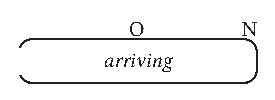
\includegraphics{figures/GrafikInceptiveAchievement.eps}
\caption{Phasal structure of \textit{fika}}
\label{FigureInceptiveAchievement}
\end{center}
\end{figure}

As for \textit{aga} \lq find', in the simple present this verb has a habitual/generic\is{aspect!habitual}\is{aspect!generic} and a \isi{futurate} reading, but no progressive one (\ref{exAcuteAchievementPRS}), which indicates the lack of a lexical Onset phase. Accordingly, the simple present in the complement of the persistive aspect auxiliary does not have a single event reading (\ref{exAcuteAchievementPersPRS}).

\begin{exe}
\ex \label{exAcuteAchievementPRS}
 \gll tʊ-kw-ag-a ɪɪ-fungulo jɪ-lɪ paa-meesa\\
\textsc{1pl}-\textsc{prs}-find-\textsc{fv} \textsc{aug}-key(9)(<SWA) 9-\textsc{cop} 16-table(9)(<SWA)\\
\glt 1. \lq We will find that a/the key is on a/the table (e.g. thus we have 
been informed).'\\
2. \lq We find that a/the key is on a/the table (e.g. each time we search for it).'

\ex \label{exAcuteAchievementPersPRS}\gll tʊ-kaalɪ tʊ-kw-ag-a bi-kʊ-ly-a\\
\textsc{1pl}-\textsc{pers} \textsc{1pl}-\textsc{prs}-find-\textsc{fv} 
2-\textsc{prs}-eat-\textsc{fv}\\
\glt \lq We still find them eating (frequently).'\\
not: \lq We are still finding them eating (sic!).'
\end{exe}

Further proof of the lack of an Onset phase is found in the facts that \textit{aga} is incompatible with the periphrastic progressive (\ref{exAcuteAchievementProg}) and that it does not have a single event reading with the ingressive \textit{anda} (\ref{exAcuteAchievementAnda}):
\begin{exe}
\ex[*]{\label{exAcuteAchievementProg}\gll tʊ-lɪ pa-kw-ag-a bi-kʊ-ly-a\\
\textsc{1pl}-\textsc{cop} 16-15-find-\textsc{fv} 2-\textsc{prs}-eat-\textsc
{fv}\\
\glt (intended: \lq We are about to find them eating.')}

\ex[]{\label{exAcuteAchievementAnda}\gll tw-and-ile ʊ-kw-ag-a bi-kʊ-ly-a\\
\textsc{1pl}-start-\textsc{pfv} \textsc{aug}-15-find-\textsc{fv} 2-\textsc
{prs}-eat-\textsc{fv}\\
\glt \lq We have begun to find them eating (e.g. each time we pass).'\\
not: \lq We have begun to find them eating (right now).'}
\end{exe}

The perfective aspect with \textit{aga }denotes that the eventuality has passed (\ref
{exAcuteAchievementPFV}). The incompatibility of perfective aspect with persistive aspect shows that no Coda phase is encoded (\ref{exAcuteAchievementPersPFV}).

\begin{exe}
\ex[]{\label{exAcuteAchievementPFV} \gll tw-ag-ile bi-kʊ-ly-a\\
\textsc{1pl}-find-\textsc{pfv} 2-\textsc{prs}-eat-\textsc{fv}\\
\glt \lq We have found them eating.'}

\ex[*]{\label{exAcuteAchievementPersPFV}\gll tʊ-kaalɪ tw-ag-ile bi-kʊ-ly-a\\
\textsc{1pl}-\textsc{pers} \textsc{1pl}-find-\textsc{pfv} 2-\textsc{prs}-eat-
\textsc{fv}\\
\glt (intended: \lq We are still informed that they are eating.')}
\end{exe}

The time-span phrase \lq take X time' denotes the time elapsing before the 
change-of-state:
\begin{exe}
\ex \gll tw-eg-ile a-ka-balɪlo a-ka-tali ʊ-kw-ag-a ɪɪ-fungulo jɪ-lɪ paa-meesa
\\
\textsc{1pl}-take-\textsc{pfv} \textsc{aug}-12-time \textsc{aug}-12-long  \textsc{aug}-15-find-\textsc{fv} \textsc{aug}-key(9)(<SWA) 9-\textsc{cop} 16-table(9)(<SWA)\\
\glt \lq We took a long time to find that a/the key is on a/the table.'
\end{exe}

Lastly, \textit{mala} \lq finish' cannot be used with \textit{fika} (\ref{exAcuteAchievementsMala}) and \textit{leka} \lq cease, stop' does not have a single event reading (\ref{exAcuteAchievementsLeka}).
\begin{exe}
\ex[*]{\label{exAcuteAchievementsMala}\gll tʊ-mal-ile ʊ-kw-ag-a ɪɪ-fungulo 
jɪ-lɪ paa-meesa\\
\textsc{1pl}-finish-\textsc{pfv} \textsc{aug}-15-find-\textsc{fv}  \textsc
{aug}-key(9) 9-\textsc{cop} 16-table(9)\\
\glt (intended: \lq We're done finding that a/the key is on the table (sic!).')}
\ex[]{\label{exAcuteAchievementsLeka}\gll tʊ-lek-ile ʊ-kw-ag-a ɪɪ-fungulo jɪ-lɪ paa-meesa\\
\textsc{1pl}-cease-\textsc{pfv} \textsc{aug}-15-find-\textsc{fv} \textsc{aug}-key(9) 9-\textsc{cop} 16-table(9)\\
\glt \lq We no longer find that a/the key is on the table'\\
not: \lq We have ceased to be finding that a/the key is on the table (sic!).'}
\end{exe}

To summarize, \textit{aga} differs from the other achievements in that it encodes neither an Onset nor a Coda phase, but only a punctual change-of-state. That is, it corresponds to the Vendlerian\ia{Vendler, Zeno} definition of achievements; see \sectref{AristotelianAspect} for discussion. Its phasal structure can be schematized as in \figref{FigureAcuteAchievement}.

\begin{figure}[h]
\begin{center}

\includegraphics{figures/GrafikAcuteAchievement.eps}
\caption{Phasal structure of \textit{aga}}
\label{FigureAcuteAchievement}
\end{center}
\end{figure}

\is{aspect!Aristotelian|)}
\is{aspect!perfective|)}\is{aspect!imperfective|)}\is{aspect!progressive|)}\is{aspect!persistive|)}\is{auxiliary|)}\is{phasal verbs|)}\is{simple present|)}\is{phase!Onset phase|)}\is{phase!Nucleus phase|)}\is{phase!Coda phase|)}
 \chapter{Tense and aspect constructions 1: present and past tense}\label{TenseAspectConstructions}
\largerpage
\section{Introduction}
In this and the following two chapters, constructions expressing \isi{tense} and grammatical aspect\is{aspect!grammatical} will be described. This chapter contains a general overview of tense and aspect in Nyakyusa, followed by a discussion of negation\is{negative} (\sectref{Negations}) and an investigation into two recurring aspectual suffixes, which show considerable morphophonemic alternation (\sectref{AlternationsIPFVaga}, \ref{Imbrication}). Its main body consists of a description of present and past tense constructions. This description is divided into constructions consisting of just the inflected verb (\sectref{SimpleConstructions}) and \isi{auxiliary} or compound constructions (\sectref{ComplexConstructions}). What is for convenience termed \lq present tense'\is{tense!present} throughout this study can be understood as having non-past reference. This is discussed in \sectref{PRSasNonPST}. Note that the dedicated narrative markers,\is{narrative markers} though they have past tense\is{tense!past} reference, will be dealt with separately in Chapter \ref{NarrativeMarkers}.

\section{Overview of tense and aspect in Nyakyusa}
A key element of the Nyakyusa TMA system in the present\is{tense!present} (non-past) and past tense\is{tense!past} is the opposition between imperfective\is{aspect!imperfective} and perfective aspect.\is{aspect!perfective} The use of grammatical aspect\is{aspect!grammatical} is closely linked to the lexical opposition between inchoative\is{inchoative verbs} and non-inchoative verbs (see Chapter \ref{AspectualClassification}). A central element here is the completion of the Nucleus phase\is{phase!Nucleus phase} of an eventuality, which is discussed in \sectref{PerfectivityCompletion}.  As each of the major present and past tense\is{tense!present}\is{tense!past} constructions is also marked for aspect, neither \isi{tense} nor grammatical aspect\is{aspect!grammatical} can be considered primary. Instead, when linguistically construing  a given state-of-affairs, a speaker of Nyakyusa has to decide on both the temporal dimension\is{tense} (\sectref{Tense}) as well as the aspectual vantage point (\sectref{Aspect})\is{aspect!grammatical} in relation to the verb's inherent aspectual potential\is{aspect!Aristotelian} (\sectref{AristotelianAspect}).

Concerning constructions with future time reference, which build on the simple present,\is{simple present} as well as the subjunctive\is{mood!subjunctive} and desiderative moods,\is{mood!desiderative} Nyakyusa rather has an opposition between aspectually neutral and imperfective aspect,\is{aspect!imperfective} where the latter frequently also adds modal\is{modality} nuances.

\section{Negation in Nyakyusa}\label{Negations}
\is{negative|(}In \sectref{SimpleConstructions}, \ref{ComplexConstructions}, \ref{Subjunctive}, the description of each affirmative construction will be followed by its negative counterpart. As has been pointed out by \citet{ContiniMoravaE1989}, among others, the semantic relationship between affirmative and negative forms is not a straightforward one. Nevertheless, when language assistants were asked for the negative equivalent of a given form, they responded readily and unanimously (see also \citealt[196]{NurseD2008}). Negation in Nyakyusa shows some uncommon characteristics, however, which deserve a short discussion.

Nyakyusa has three negative prefixes: \textit{ti}-, \textit{ka}- and \textit{nga}-. All three stand in the  post-initial slot. Their distribution is delimited along two major lines: mood and temporal reference. The \textit{nga}- negation is limited to the negative subjunctive (\sectref{NegativeSubjunctive}). Of the remaining two negative prefixes, \textit{ka}- is used in constructions that make reference to a point of time prior to the moment of speech,\footnote{The moment of speech is to be understood here as the default reference point.} while \textit{ti}- occurs solely in the present and in futurates.\footnote{This contrasts with Ndali, which has \textit{ta}- for non-pasts as well as pasts (\citealt{BotneR2008}; \citealt{SwillaI1998}). The \ili{Ngonde} varieties described by \citet{KishindoP1999} and \citet{LabroussiC1998} seem to exhibit a certain variability and stand between Nyakyusa and \ili{Ndali} with regards to the negative markers.} The apparent exception is the negative copula, which for the non-generic\is{aspect!generic} present is \textit{ka-j-a} (\sectref{Copulae}). However, this can clearly be attributed to its origin in the negation of \lq become', which, depending on the context, is still a possible reading. What has just been outlined is uncommon in two ways. First, in the majority of those Bantu languages having more than one negative marker, these occur in different positions in the verbal word. Second, in those Bantu languages with three negative markers, the typical distribution is main clause vs. subjunctive vs. relative clause \citep[184--191]{NurseD2008}.

A common typological criterion concerning verbal negation is symmetry. As \citet[556]{MiestamoM2007} defines it, ``symmetric negative constructions do not differ from non-negatives in any other way than by the presence of the negative marker(s)''.\footnote{More precisely, Miestamo in the quoted section is concerned with \lq standard negation', that is, the negation of declarative verbal main clauses, excluding, for instance, existential or copula clauses or non-declarative ones such as the imperative.} While negation in Nyakyusa is mostly symmetric, as can be seen from the sample constructions in \tabref{tableSymmetricNegation}, there are several cases of asymmetric negation; see \tabref{tableAsymmetricNegation}. There are also cases of syncretism, where more than one affirmative paradigm shares a common negative counterpart; see \tabref{tableSyncretismNegation}. \citet{MiestamoM2005} calls the latter ``paradigmatic A/Cat asymmetry''.


\begin{table}[H]
\begin{center}
\begin{tabular}{ccc}
\lsptoprule 
& \footnotesize{Affirmative} & \footnotesize{Negative}\\ 
\midrule 
Simple present & \textit{kʊ}-\textsc{vb}-\textit{a} & \textit{ti}-\textit{kʊ}-\textsc{vb}-\textit{a}\\ 
Past perfective & \textit{a(lɪ)}-\textsc{vb}-\textit{ile} & \textit{ka}-\textit{a(lɪ)}-\textsc{vb}-\textit{ile}\\ 
Past imperfective & \textit{a}-\textsc{vb}-\textit{aga} & \textit{ka}-\textit{a}-\textsc{vb}-\textit{aga}\\ 
\lspbottomrule
\end{tabular} 
\caption{Cases of symmetric negation}
\label{tableSymmetricNegation}
\end{center}
\end{table}

\begin{table}[H]
\begin{center}
\begin{tabular}{ccc}
\lsptoprule 
& \footnotesize{Affirmative} & \footnotesize{Negative}\\ 
\midrule 
Present perfective & \textit{ø}-\textsc{vb}-\textit{ile} & \textit{ka}-\textsc{vb}-\textit{a}\\ 
Subjunctive & \textit{ø}-\textsc{vb}-\textit{e}(\textit{ge}) & \textit{nga}-\-\textsc{vb}-\textit{a}(\textit{ga})\\
Narrative tense & \textit{lɪnkʊ}-\textsc{vb}-\textit{a} & \textit{lɪnkʊ}-\textit{sit}-\textit{a} + infinitive\\
\lspbottomrule
\end{tabular} 
\caption{Cases of asymmetric negation}
\label{tableAsymmetricNegation} 
\end{center}
\end{table}

\begin{table}[H]
\begin{center}
\begin{tabular}{cc}
\lsptoprule 
\footnotesize{Affirmative} & \footnotesize{Negative}\\ 
\midrule 
Simple present & \multirow{2}{*}{Negative present}\\
Present progressive & \\ \hline
Past imperfective & \multirow{2}{*}{Negative past imperfective}\\
Past progressive & \\ \hline
Subjunctive & \multirow{2}{*}{Negative subjunctive}\\
Distal/itive subjunctive& \\
\lspbottomrule
\end{tabular}
\caption{Syncretism in negation}
\label{tableSyncretismNegation}  
\end{center}
\end{table}
\is{negative|)}

\newpage 
\section{Morphophonology of common TMA suffixes}
\subsection{Alternations of imperfective -\textit{aga}}\label{AlternationsIPFVaga} 
\is{aspect!imperfective|(}The imperfective suffix surfaces as -\textit{aga} in those paradigms characterized by the default final vowel -\textit{a}, and as -\textit{ege} in the affirmative subjunctive.\is{mood!subjunctive} The defective verb \textit{tɪ} (\sectref{defectiveti}) occurs as \textit{tɪgɪ}.
\begin{exe}
\ex
\begin{tabular}[t]{ll}
\textit{twajobaga}&`we were speaking'
\\\textit{tʊjobege}&\lq we should be speaking'
\\\textit{twatɪgɪ}&`we were saying'
\end{tabular}
\end{exe}

When one of the clitics\is{enclitic} (see \sectref{PostfinalClitics}) \textit{=po}, \textit{=mo} or \textit{=ko} (independent of their specific function) or \textit{=kʊ} \lq where' follows, the velar segment is prenasalized (\ref{exEncliticsAgaPrenasalized}). With the \isi{enclitic} form of \textit{ki} `what', no prenasalization takes place (\ref{exEncliticsAgaKiNotPrenasalized}).
\begin{exe}
\ex\label{exEncliticsAgaPrenasalized}
\begin{tabbing}
\textit{gwabʊʊk\textbf{anga}kʊ}x\=(\degree ba-a-sook-aga=mo)x\=\kill
\textit{baaswɪl\textbf{anga}po}\>(\degree ba-a-swɪl-aga=po)\>`they were raising there (class 16)'\\
\textit{biigal\textbf{anga}ko}\>(\degree ba-a-igala-aga=ko)\>`they were closing there (class 17)'\\
\textit{baasook\textbf{anga}mo}\>(\degree ba-a-sook-aga=mo)\>`they were going outside (class 18)'\\
\textit{ʊswɪl\textbf{enge}po}\>(\degree ʊ-swɪl-ege=po)\>`you should raise there (class 16)'\\
\textit{gwigal\textbf{enge}ko}\>(\degree ʊ-igal-ege=ko)\>`you should close there (class 17)'\\
\textit{ʊsook\textbf{enge}mo}\>(\degree ʊ-sook-ege=mo)\>`you should go outside (class 18)'\\
\textit{gwabʊʊk\textbf{anga}kʊ}\>(\degree ʊ-a-bʊʊk-aga=kʊ)\>`Where were you going?'\\
\textit{mbʊʊk\textbf{enge}kʊ}\>(\degree n-bʊʊk-ege=kʊ)\>`Where should I go?'
\end{tabbing}
\ex\label{exEncliticsAgaKiNotPrenasalized}\begin{tabbing}
\textit{gwabʊʊk\textbf{anga}kʊ}x\=(\degree ba-a-sook-aga=mo)x\=\kill
\textit{gwabomb\textbf{aga}ki}\>(\degree ʊ-a-bom-aga=ki)\>`What were you doing?'
\end{tabbing}
\end{exe}
\is{aspect!imperfective|)}
\subsection{Perfective -\textit{ile} and its variants}\label{Imbrication} 
\is{imbrication|(}\is{aspect!perfective|(}
Perfective stems in Nyakyusa are subject to complex allomorphic variation. With the widespread Bantu suffix -\textit{ile} as the underlying form, surface forms are diverse and in many cases show characteristics of fusional morphology. Before going into detail with the numerous shapes perfective stems take and the phonological and morphological factors triggering the choice of these, it should be stated that perfective stem formation can be understood as variation on three re-occurring themes. The first and most straightforward is suffixation of -\textit{ile}:
\begin{exe}
\ex
\begin{tabular}[t]{@{}>{\itshape}llll}
\textit{nwa}&`drink'& > \textit{nwile}
\\\textit{gana}&`love'& > \textit{ganile}
\\\textit{nyunyuuta}&`whine'& > \textit{nyunyuutile}
\end{tabular}
\end{exe} 
The second theme is called \textit{imbrication}, a term coined by \citet{BastinY1983}. In its prototypical form, imbrication consists of infixing -\textit{i}- before the last base consonant and suffixing -\textit{e}. The rules of word-internal hiatus solution (\sectref{HiatusSolution}) apply.
\begin{exe}
\ex
\begin{tabular}[t]{@{}>{\itshape}llll}
\textit{lwasya}&`nurse the sick, care for'& > \textit{lwa<\textbf{i}>sy-\textbf{e}}& > \textit{lwesye}
\\\textit{bukuka}&`flare'& > \textit{buku<\textbf{i}>k-\textbf{e}} & > \textit{bukwike}
\\\textit{ambɪlɪla}&`receive; entertain guests'& > \textit{ambɪlɪ<\textbf{i}>l-\textbf{e}}& > \textit{ambɪliile}
\end{tabular}
\end{exe} 
A third theme will be referred to as \textit{copying}. In its basic form, copying consists of a surface alternation /-CG/ $\rightarrow$ /-CiiCGe/, where CG stands for the base-final consonant plus a following glide. Although at first this looks like a case of reduplication,\is{reduplication} the discussion below will show that these forms can best be explained by assuming \isi{templatic} requirements of certain types of stems.
\begin{exe}
\ex
\begin{tabular}[t]{@{}>{\itshape}lll}
\textit{busya}&`return (tr.)'& > \textit{busiisye}
\\\textit{pʊfya}&`whistle'& > \textit{pʊfiifye}
\\\textit{ibwa}&`forget'& > \textit{ibiibwe}
\end{tabular}
\end{exe}

The following in-depth description of perfective stem formation will be structured according to the syllable count of the verbal base, as this is a major conditioning factor and each syllable count can be associated with a default process. Some of the regularities outlined have already been recognized by \citet{BergerP1938}. However, the present data shows a number of deviations from Berger's analysis, which in most cases can be attributed to the greater quantity of data considered.\footnote{Berger himself recognizes the limits of his corpus and that the transcription of some of his second-hand data is rather dubious. Nevertheless, his work is a valuable point of departure. Apart from \citet{BergerP1938}, the forms cited in \citet{FelbergK1996} have been taken as an indication of where to look for regularity and variation. All forms stemming from those sources that were felt to be suspicious have been checked in elicitation.} This is based on the examination of some 1600 verbal bases for which perfective stems were available at the time of writing this section.

\subsubsection{Monosyllabic verbs}
% \todo{is the extra tab in fwile intended?}
With monosyllabic verbs, -\textit{ile} is suffixed. The general rules of vowel juxtaposition apply (\sectref{HiatusSolution}). Defective \textit{tɪ} (\sectref{defectiveti}) yields \textit{tile}, which is often reduced to [tʰi̯ɛ]. Likewise, \textit{jile} is often heard as [ɟi̯ɛ]. In both cases, \isi{stress} remains on the stem syllable.
\begin{exe}
%\begin{multicols}{2}
\ex
\begin{tabbing}
\textit{kya}x \=`dawn; cease\= to rain'x\= > \textit{kiile}\kill
\textit{pa}\>`give'\> > \textit{peele}\\
\textit{ja}\>`be(come)'\> > \textit{jile}\\
\textit{tɪ}\>`say'\> > \textit{tile} \\
\textit{twa}x\=`be plenty (esp. fish)'x\= > \textit{twile}\kill %Unsinnszeile für neue tabs
\textit{fwa}\>`die'\> > \textit{fwile} \\
\textit{gwa}\>`fall'\> > \textit{gwile} \\
\textit{kwa}\>`pay dowry'\> > \textit{kwile} \\% \columnbreak
\textit{lwa}\>`fight'\>\> > \textit{lwile} \\ 
\textit{mwa}\>`shave'\>\> > \textit{mwile} \\
\textit{nwa}\>`drink'\>\> > \textit{nwile} \\
\textit{swa}\>`spit; forgive'\>\> > \textit{swile} \\
\textit{twa}\>`be plenty (esp. fish)'\>\> > \textit{twile}\\
\textit{kya}\>`dawn; cease to rain'\>\> > \textit{kiile}\\
%\end{tabbing}
%\end{multicols}
%\end{exe}
%\clearpage
%\begin{exe}
%\sn
%\begin{tabbing}
%\textit{pya}x\=`be(come) burnt'x\= > \textit{piile}\kill
\textit{lya}\>`eat'\> > \textit{liile} \\
\textit{nia}\>`defecate'\> > \textit{niile} \\
\textit{pya}\>`be(come) burnt'\> > \textit{piile}\\
\textit{sya}\>`grind'\> > \textit{siile}
\end{tabbing}
\end{exe}

\subsubsection{Disyllabic verbs} \label{ImbricationDisyllabic}
Disyllabic verbs show by far the most complex variation. Suffixation of -\textit{ile}
can be considered the default case:
\begin{exe}
\ex
\begin{tabular}[t]{@{}>{\itshape}lll}
\textit{goga}&`kill'& > \textit{gogile}\\
\textit{keeta}&`watch'& > \textit{keetile}\\
\textit{konga}&`follow'& > \textit{kongile}\\
\textit{ʊla}&`buy'& > \textit{ʊlile}
\end{tabular}
\end{exe}


With disyllabic applicatives (that is, applicatives of monosyllabic roots) -\textit{iile}, with a long morpheme-initial vowel,\is{vowels!length} is suffixed.
\begin{exe}
\ex
\begin{tabbing}
\textit{nwela}x\=`defecate with/at/for'x\=\kill%unsinnige Zeile nur fuer tabs
\textit{peela}\>`give off'\> > \textit{peeliile}\\
\textit{jɪɪla}\>`be in a condition'\> > \textit{jɪɪliile}\\
\textit{lɪɪla}\>`eat with/at/for'\> > \textit{lɪɪliile}\\
\textit{niela}\>`defecate with/at/for'\> > \textit{nieliile}\\
\textit{syela}\>`grind with/at/for'\> > \textit{syeliile}\\
\textit{gwɪla}\>`fall with/to/for'\> > \textit{gwɪliile}\\
\textit{nwela}\>`drink with/at/for'\> > \textit{nweliile}
\end{tabbing}
\end{exe}

\largerpage
With disyllabic fossilized passives\is{passive!fossilized} (\sectref{FossilizedPassive}), -\textit{il}- is infixed before the glide and -\textit{e} is suffixed (\ref{exFossilizedPassivesImbrication}). These verbs thus occupy an intermediate position between suffixing and imbrication in the strict sense.\footnote{\citet{SchumannK1899} and \citet{BergerP1938} note that these verbs form their perfective stem with long -\textit{iilwe}.\is{vowels!length} This could not be confirmed and might be due to diatopic variation or due to confusion with their applicativized forms.} The same holds for one of the perfective stem variants of \textit{lɪɪgwa} \lq be eaten' (\ref{exlIIgwaSemiImbrication}).
\begin{exe}
\ex\label{exFossilizedPassivesImbrication}
\begin{tabbing}
\textit{nyonywa}x\=`be burdened'x\= > \textit{nyonyilwe}\kill
\textit{babwa}\>`be in pain'\> > \textit{babilwe}\\ 
\textit{gogwa}\>`dream'\> > \textit{gogilwe}\\
\textit{milwa}\>`drown'\> > \textit{mililwe}\\
\textit{nyonywa}\>`desire'\> > \textit{nyonyilwe}\\
\textit{syʊkwa}\>`miss sadly'\> > \textit{syʊkilwe}\\
\textit{tolwa}\>`be burdened'\> > \textit{tolilwe}
\end{tabbing}
\ex \label{exlIIgwaSemiImbrication}
\begin{tabbing}
\textit{nyonywa}x\=`be burdened'x\= > \textit{nyonyilwe}\kill
\textit{lɪɪgwa}\>`be eaten'\> > \textit{lɪɪgilwe} (also \textit{lɪɪgiigwe}, see below)
\end{tabbing}
\end{exe}

Verbs of the shapes CG\textit{al} and CG\textit{an} induce imbrication (\ref{exImbricationalaman}). One exception to this rule is attested (\ref{exCGAXloansNoImbrication}). The unusual sequence /ŋw/ indicates that the verb \textit{ng'wala} might be a \ili{Ndali} loan.\footnote{Cf. pairs such as Nyakyusa \textit{nwa}, \ili{Ndali} \textit{ŋwa} \lq drink' < PB *\textit{ɲwó}.} \citet{BergerP1938} further lists \textit{nywama} > \textit{nyweme}, thus CG\textit{am}. Of the speakers consulted, several did not know this verb at all. Those familiar with it unanimously gave \textit{nywamile} as their first answer. Some accepted \textit{nyweme} as a variant perfective stem, whereas it was rejected by others (\ref{exCGAXnywama}). The only other verb of the shape in question is \textit{kwama} \lq be(come) stuck', an obvious loan from Swahili, which has the perfective stem \textit{kwamile}  not *\textit{kweme}. As the examples in (\ref{exCGACnoImbrication}) illustrate, other CG\textit{a}C shapes do not induce imbrication.

\begin{exe}
\ex
\begin{tabbing}
\textit{nywama}x\=\lq resemble; be enough'x\=\kill  %unsinnige Zeile fur Tabulatoren
\textit{fwala}\>`wear; receive salary'\> > \textit{fwele}
\\\textit{syala}\>`remain'\> > \textit{syele}\label{exImbricationalaman}
\\\textit{fwana}\>\lq resemble; be enough'\> > \textit{fwene}
\\\textit{lwana}\>`quarrel'\> > \textit{lwene}
\end{tabbing}
\ex\label{exCGAXloansNoImbrication}
\begin{tabbing}
\textit{nywama}x\=\lq resemble; be enough'x\=\kill  %unsinnige Zeile fur Tabulatoren
\textit{ng'wala}\> \lq scratch with claws'\> > \textit{ng'walile} (not *\textit{ng'wele})
\end{tabbing}
\ex\label{exCGAXnywama}
\begin{tabbing}
\textit{nywama}x\=\lq resemble; be enough'x\=\kill  %unsinnige Zeile fur Tabulatoren
\textit{nywama}\>`enlarge (intr.); chase'\> > \textit{nywamile} (also \textit{nyweme})
\end{tabbing}
\ex\label{exCGACnoImbrication}
\begin{tabbing}
\textit{nywama}x\= \lq resemble; be enough'x\=\kill  %unsinnige Zeile fur Tabulatoren
\textit{fyata}\>`fasten'\> > \textit{fyatile} (not *\textit{fyete})
\\\textit{kwaba}\>`take'\> > \textit{kwabile} (not *\textit{kwebe})
\end{tabbing}
\end{exe}

The verb \textit{baala} \lq increase, thrive' shows variation between an imbricating and a suffixing form (\ref{exBaalaImbrication}). This must be considered an idiosyncrasy, as no other verb of the shape /Caal/ has an imbricating perfective stem (\ref{exCaalNoImbrication}).

\begin{exe}
\ex\label{exBaalaImbrication}
\begin{tabbing}
\textit{paala}x\= \lq get drunk, be drunk'x\=\kill  %unsinnige Zeile fur Tabulatoren
\textit{baala}\> \lq increase; thrive' \>> \textit{beele} / \textit{baalile}
\end{tabbing}
\ex\label{exCaalNoImbrication}
\begin{tabbing}
\textit{paala}x\= \lq get drunk, be drunk'x\= > \textit{paalile}x\=\kill  %unsinnige Zeile fur Tabulatoren
\textit{gaala}\> \lq get drunk, be drunk' \> > \textit{gaalile}\>(not *\textit{geele})\\
\textit{paala}\> \lq invite' \> > \textit{paalile}\>(not *\textit{peele})\\
\textit{saala}\> \lq be(come) happy' \> > \textit{saalile}\>(not *\textit{seele})
\end{tabbing}
\end{exe}

Two further disyllabic verbs must be considered irregular: \textit{manya} \lq know' and \textit{bona} \lq see'. These trigger imbrication although no other regularity can account for this. Further, \textit{bona} does not yield *\textit{bwine} as would be expected from the rules of vowel coalescence.
\begin{exe}
\ex
\begin{tabular}[t]{@{}>{\itshape}lll}
\textit{manya} &`know' & > \textit{meenye}
\\\textit{bona} & `see' & > \textit{bwene}
\end{tabular}
\end{exe}

\is{causative|(}
Disyllabic causatives trigger copying, yielding (C)(G)V\textit{siisye} if the base ends in /sy/ and (C)(G)V\textit{fiifye} if the base ends in /fy/. This holds for causatives\is{causative} of monosyllabic roots\is{root} formed with the long causative\textsubscript{2} \mbox{-\textit{ɪsi} }(\ref{exCopyingBiCausativeLong}), as well as for those causatives formed with the short causative\textsubscript{1} \mbox{-\textit{i}} on disyllabic verbs (\ref{exCopyingBiCausativeShort}); see \sectref{TwoCausatives} for a discussion of the two causatives. Causatives with base-final nasals also have a perfective stem of the shape (C)VN\textit{iisye} (\ref{exDisyllabicCausativesWithNasal}), which shows that synchronically speaking this is not a rule of reduplication,\is{reduplication} as it might appear at first sight. A historic scenario for this alternation is provided by \citet{HymanL2003b}. He argues that its origin most probably lies in imbrication plus a cyclic application of \isi{spirantization} through the causative\textsubscript{1} -\textit{i} (\sectref{Causative1}), thus yielding (C)(G)V\textit{siisye} for base-final spirantizing\is{spirantization} oral linguals. This then came to be re-analysed as a process of reduplication,\is{reduplication} yielding (C)(G)V\textit{fiifye} with base-final oral labials. Lastly, this turned into a phonological pattern requirement\is{templatic} for disyllabic causative stems to end in -\textit{ii}\{\textit{s},\textit{f}\}\textit{ye}, hence the extension to final nasals (and causatives of monosyllabic verbs, which are not discussed by Hyman).

Note that disyllabic causatives derived from the verbs of the shape CG\textit{a}\{\textit{l}, \textit{n}\} discussed above are excluded from this process. As with their underlying bases,\is{base} imbrication takes place (\ref{exNoImbricationDisyllabicanlm}). The causative of \textit{baala}, \textit{baasya} \lq increase (tr.)' shows variation just like its underlying root,\is{root} and is attested with both imbricating and copying forms (\ref{exImbricationBaasya}).

\begin{exe}
\ex Causatives of monosyllabic roots:\\
\label{exCopyingBiCausativeLong}
\begin{tabular}[t]{@{}>{\itshape}lll}
%\textit{gw-ɪsi-a}x\=`overturn; throw down'x\= > \textit{gwɪsiisye}\kill
\textit{lw-ɪsi-a}&`make fight'& > \textit{lwɪsiisye}
\\\textit{gw-ɪsi-a}&`overturn; throw down'& > \textit{gwɪsiisye}
\end{tabular}
\ex Disyllabic causatives with -\textit{i}:\\
\label{exCopyingBiCausativeShort}
\begin{tabular}[t]{@{}>{\itshape}llll}
%\textit{pyʊfya}x\=(\degree pyʊp-i-a)x\=`warm, heat up'x\= > \textit{pyʊfiifye}\kill
\textit{bosya}&(\degree bol-i-a)&`cause to rot'& > \textit{bosiisye}
\\\textit{pyʊfya}&(\degree pyʊp-i-a)&`warm, heat up'& > \textit{pyʊfiifye}
\end{tabular}
\ex Disyllabic causatives with final nasal:\\
\label{exDisyllabicCausativesWithNasal}
\begin{tabular}[t]{@{}>{\itshape}lll}
%\textit{taam-y-a}x\=`put out, extinguish'x\=\kill%Unsinnige Zeile nur fuer Tabulatoren
\textit{pon}-\textit{i}-\textit{a}&`greet; visit'& > \textit{poniisye}
\\\textit{an}-\textit{i}-\textit{a}&`ask'& > \textit{aniisye}
\\\textit{sim}-\textit{y}-\textit{a}&`put out, switch off'& > \textit{simiisye}
\\\textit{taam}-\textit{y}-\textit{a}&`trouble, persecute'& > \textit{taamiisye}
\end{tabular}
\ex Disyllabic causatives CG\textit{a\{l, n\}-i}:\\\label{exNoImbricationDisyllabicanlm}
\begin{tabular}[t]{@{}>{\itshape}llll}
%\textit{lwania}x\=(\degree lwan-i-a)x\=`confront; make quarrel'x\=\kill
\textit{lwasya}&(\degree lwal-i-a)&`nurse the sick, care for'& > \textit{lwesye}
\\\textit{syasya}&(\degree syal-i-a)&`leave over'& > \textit{syesye}
\\\textit{fwania}&(\degree fwan-i-a)&`match; reconcile'& > \textit{fwenie}
\\\textit{lwania}&(\degree lwan-i-a)&`confront; make quarrel'& > \textit{lwenie}
\end{tabular}
\ex Causative of \textit{baala}:\label{exImbricationBaasya}\\
\begin{tabular}[t]{@{}>{\itshape}llll}
\textit{baasya}&(\degree baal-i-a)&`increase (tr.)'& > \textit{beesye} / \textit{baasiisye}
\end{tabular}
\end{exe}
\is{causative|)}
Some other verbs of the shape (C)VCG form their perfective stems by copying (C\textsubscript{1})VC\textsubscript{2}G $\rightarrow$ (C\textsubscript{1})VC\textsubscript{2}-\textit{ii}-C\textsubscript{2}G-\textit{e}.\footnote{For \textit{bɪfwa}, \citet{BergerP1938} and \citet{FelbergK1996} list \textit{bɪfwifwe} as a variant, while for \textit{ibwa} \citet{BergerP1938} also has \textit{ibwibwe}; \citet{NurseD1979} has \textit{okya} > \textit{okyokye}, thus (C\textsubscript{1})(G)VC\textsubscript{2}G $\rightarrow$ (C\textsubscript{1})VC\textsubscript{2}GV-\textit{i}-C\textsubscript{2}G-\textit{e}. All the speakers consulted in the present study rejected these forms, which seems to be a case of diatopic\is{dialects} variation (both Felberg's and Berger's main sources stem from more southern varieties). \citet{FelbergK1996} further lists a copying stem for \textit{miimwa} \lq crave; envy', which was also rejected.}
\begin{exe}
\ex
\begin{tabular}[t]{@{}>{\itshape}llll}
\textit{bɪfwa}&`ripen'& > \textit{bɪfiifwe}
\\\textit{ibwa}&`forget'& > \textit{ibiibwe}
\\\textit{ikya}&`be(come) confident'& > \textit{ikiikye}
\\\textit{okya}&`grill, burn'& > \textit{okiikye}
\\\textit{lɪɪgwa}&`be eaten'& > \textit{lɪɪgiigwe} (also \textit{lɪɪgilwe}; see above)
\\\textit{peegwa}&`be given'& > \textit{peegiigwe}
\end{tabular}
\end{exe} 

\subsubsection{Tri- and polysyllabic verbs}
With verbs that have three or more syllables, imbrication is the default. %evtl je vokal nur eins
\begin{exe}
\ex%hier muss es tabbing sein, da das sonst mit dem Seitenumbruch nicht funktioniert. Das longtable-Paket scheitert daran, die Tabelle oben in dem Beispiel auszurichten
\begin{tabbing}
\textit{bʊmbʊlʊka}x\='be slackened, give in'x\=\kill%unsinnszeile für tabs
\textit{aganila}\>`meet'\> > \textit{aganiile} \\
\textit{gundamika}\>`bend over'\> > \textit{gundamiike}\\
\textit{guulɪla}\>`wait for'\> > \textit{guuliile}\\
\textit{itɪkɪla}\>`answer; approve'\> > \textit{itɪkiile}\\ 
\textit{geleka}\>`thatch, pile'\> > \textit{geliike}\\
\textit{koolela}\>`call; name; bid'\> > \textit{kooliile} \\
\textit{bagala}\>`carry on shoulder'\> > \textit{bageele} \\
\textit{fumbata}\>`(en)close'\> > \textit{fumbeete}\\
\textit{jobana}\>`converse'\> > \textit{jobeene}\\
\textit{honyoka}\>`be slackened; give in'\> > \textit{honywike}\\
\textit{kosomola}\>`cough'\> > \textit{kosomwile}\\
\textit{bʊmbʊlʊka}\>`get well, be healed'\> > \textit{bʊmbʊlwike}\\
\textit{fyʊtʊla}\>`pull out'\> > \textit{fyʊtwile}\\
\textit{fujula}\>`humiliate, dishonour'\> > \textit{fujwile}\\
\textit{amula}\>`answer'\> > \textit{amwile}
\end{tabbing}
\end{exe}

With the long\is{vowels!length} allomorph of the \isi{reciprocal} -\textit{aan} and its causativized/plur\-action\-al\is{causative}\is{pluractional} form \mbox{-(\textit{ɪs})\textit{aani}}, imbrication takes place:

\begin{exe}
\ex
\begin{tabular}[t]{@{}>{\itshape}lll}
\textit{bʊngaana}&`(be) assemble(d)'& > \textit{bʊngeene}\\
\textit{bʊngaania}&`gather'& > \textit{bʊngeenie}\\
\textit{lʊngaana}&`join together (intr.)'& > \textit{lʊngeene}\\
\textit{lʊngɪsaania}&`put together, arrange'& > \textit{lʊngɪseenie}\\
\textit{ongaana}&`be together, mixed'& > \textit{ongeene}\\
\textit{ongaania}&`mix, sum up'& > \textit{ongeenie}
\end{tabular}
\end{exe}

The verb \textit{ilaamwa} \lq disregard, doubt' shows some variation. An imbricating stem \textit{ileemwe} was observed, as well as \textit{ilaamwisye}. \citet{BergerP1938} observes a third hybrid variant \textit{ileemwisye}. With the speakers consulted, \textit{ileemwe} is the most frequent form.

All other verbs which have more than two syllables, a long rightmost vowel and that are not causatives\is{causative} form their perfective stems by suffixation of -\textit{ile}: %(\ref{exLongVowelNoImbrication}). 
\begin{exe}
\ex \label{exLongVowelNoImbrication}
\begin{tabbing}
\textit{niembeteela}x\=`wrap, conceal'x\= > \textit{niembeteelile}\kill
\textit{jɪgɪɪla}\>`shake (intr.)'\> > \textit{jɪgɪɪlile}\\
\textit{ogeela}\>`swim'\> > \textit{ogeelile}\\
\textit{niembeteela}\>`wrap, conceal'\> > \textit{niembeteelile}\\
\textit{tendeela}\>`peep, peek'\> > \textit{tendeelile}\\
\textit{kolooma}\>`grown'\> > \textit{koloomile}
\end{tabbing}
\end{exe}

With verbs that feature a base-final prenasalized plosive (recall that these predictably induce lengthening\is{vowels!length} in the preceding vowel), as well as with causatives\is{causative} having a long vowel\is{vowels!length} in the rightmost position (minus those containing the \isi{reciprocal} plus causative,\is{causative} as discussed above), variation is found. Typically, the former trigger suffixing of -\textit{ile} while the latter trigger copying, which yields \mbox{-C\textit{iisye}/}\mbox{-C\textit{iifye}}. These are the formations given by \citet{SchumannK1899} and \citet{BergerP1938} and the only ones attested in the textual data. However, at least for the verbs given in (\ref{exImbricationVariationNC}, \ref{exImbricationVariationLongCaus}), some speakers also have imbricating forms.\footnote{Given this variation and the variant forms of \textit{ilaamwa}, together with the fact that tri- and polysyllabic verbs ending in -\textit{aan(i)} induce imbrication, one might suspect a loosening constraint against imbrication with long and lengthened vowels\is{vowels!length} (in terms of moraic phonology: bimoraic vowels). \citet{FelbergK1996} lists \textit{bulunga} > \textit{bulungile} / \textit{bulwinge}, \textit{l[a]alʊʊsya} / \textit{l[a]alwsiye} (indication of vowel length\is{vowels!length} missing) and  \textit{palamaasya} > \textit{palamaasiisye} / \textit{palameesye}.}

\begin{exe}
\ex Copying with -VV\textit{\{s, f\}y}:\\
\label{exLongCausCopying}
\begin{tabular}[t]{@{}>{\itshape}lll}
malɪɪsya&`end, eliminate'& > \textit{malɪɪsiisye}
\\eneesya&`inspect, visit'& > \textit{eneesiisye}
\\balabaasya& \lq spread out (tr.); pretend'& > \textit{balabaasiisye}
\\syʊngʊʊsya&`rotate (tr.)'& > \textit{syʊngʊʊsiisye}
\\nyonyoofya&`attract, rouse desire'& > \textit{nyonyofiifye}
\end{tabular}
\ex Variation with -VNC:\label{exImbricationVariationNC}\\
\begin{tabular}[t]{@{}>{\itshape}lll}
%\textit{kung'unda}x\=`shake off; beat up; knock'x\= >\textit{kung'undile}x\= \=\kill
onanga& \lq destroy'& > \textit{onangile} / \textit{onenge}
\\tononda&`peck; dot up'& > \textit{tonondile} / \textit{tonwinde}
\\kung'unda&shake off; beat up'& > \textit{kung'undile} / \textit{kung'winde}
\\bulunga&`roll up, make round'& > \textit{bulungile} / \textit{bulwinge}
\end{tabular}
\ex Variation with -VV\textit{sy}:\\
\label{exImbricationVariationLongCaus}
\begin{tabular}[t]{@{}>{\itshape}lll}
%\textit{palamaasya}x\=`proclaim (<SWA)'x\= > \textit{palamaasiisye}x\= \kill%Unsinn, nur fuer Tabulatoren
palamaasya&`touch; grope'& > \textit{palamaasiisye} / \textit{palameesye}
\\tangaasya& \lq proclaim (<SWA)'& > \textit{tangaasiisye} / \textit{tangeesye}
\\laalʊʊsya& \lq ask'& > \textit{laalʊʊsiisye} / \textit{laalwisye}
\end{tabular}
\end{exe}

Lastly, partially reduplicated\is{reduplication} verbs that have one of the shapes \mbox{C\textsubscript{1}V\textsubscript{1}C\textsubscript{1}V\textsubscript{1}V\textsubscript{1}C\textsubscript{2}} or \mbox{C\textsubscript{1}G\textsubscript{1}V\textsubscript{1}C\textsubscript{1}G\textsubscript{1}V\textsubscript{1}C\textsubscript{2}}, where C\textsubscript{2} is an approximant or plosive, are treated as if disyllabic. The same holds for spirantized\is{spirantization} causatives\is{causative} (\sectref{Causative1}) thereof. Although for the first pattern this behaviour could also be motivated by the rightmost long vowel,\is{vowels!length} the second group shows that this is rather a function of the overall phonemic shape. It is a noteworthy fact that all the attested verbs in question can be considered onomatopoetic or de-ideophonic.\is{ideophones} A similar rule that blocks imbrication holds in \ili{Yao} P21 \citep[112, 120]{BergerP1938}. This suggests itself to be functionally motivated, in order to preserve the sound symbolism. For a discussion of how sound symbolism can motivate exceptions on the diachronic axis, see \citet[55f]{DimmendaalG2011}.
\begin{exe}
\ex Shape C\textsubscript{1}V\textsubscript{1}C\textsubscript{1}V\textsubscript{1}V\textsubscript{1}C\textsubscript{2}:
\\\begin{tabular}[t]{@{}>{\itshape}lll}
%\textit{ng'ong'oola}x\=`grimace at'x\=\kill
\textit{boboota}&`grunt'& > \textit{bobootile}
\\\textit{hohoola}&`jeer'& > \textit{hohoolile}
\\\textit{ng'ong'oola}&`grimace at'& > \textit{ng'ong'oolile}
\\\textit{nyunyuuta}&`whine'& > \textit{nyunyuutile}
\\\textit{nyinyiila}&`squint'& > \textit{nyinyiilile}
\end{tabular}
\ex Shape C\textsubscript{1}G\textsubscript{1}V\textsubscript{1}C\textsubscript{1}G\textsubscript{1}V\textsubscript{1}C\textsubscript{2}:
\\\begin{tabular}[t]{@{}>{\itshape}lll}
%\textit{mwemweka}x\=`blab, talk nonsense'x\=\kill%unsinnig, aber fuer Tabulatoren
\textit{bwabwata}&`blab, talk nonsense'& > \textit{bwabwatile}
\\\textit{bwabwaja}&`blab, talk nonsense'& > \textit{bwabwajile}
\\\textit{mwemweka}&`glitter'& > \textit{mwemwekile}
\end{tabular}
\ex Shape C\textsubscript{1}G\textsubscript{1}V\textsubscript{1}C\textsubscript{1}G\textsubscript{1}V\textsubscript{1}C\textsubscript{2}-\textit{i}\textsubscript{\textsc{caus}}:
\\\begin{tabular}[t]{@{}>{\itshape}lll}
\textit{mwemwesya}&`move around light'& > \textit{mwemwesiisye}
\\\textit{myamyasya}&`smoothen out'& > \textit{myamyasiisye}
\\\textit{i-ng'weng'wesya}&`grumble'& > \textit{i-ng'weng'wesiisye}
\\\textit{ng'wang'wasya}&`not do thoroughly'& > \textit{ng'wang'wasiisye}
\end{tabular}
\end{exe}
\is{imbrication|)}\is{aspect!perfective|)}

\label{PastNonPast}
\section{Synthetic present and past constructions} \label{SimpleConstructions}
In the following, present\is{tense!present} (non-past) and past\is{tense!past} tense constructions consisting of solely the inflected verb will be described. These are listed in \tabref{tableSimpleConstructions}.
\begin{table}[hh]
\setlength{\tabcolsep}{2pt}
\begin{tabularx}{\textwidth}{llll}
\lsptoprule
\footnotesize{Label} & \footnotesize{Shape} & \footnotesize{Example}\\
\midrule 
Simple present & \textsc{sm}\textsubscript{2}-\textit{kʊ}-\textsc{vb}-\textit{a} & \textit{tʊkʊjoba} & \lq we  speak' \\  
Negative present & \textsc{sm}-\textit{ti}-\textit{kʊ}-\textsc{vb}-\textit{a} &  \textit{tʊtikʊjoba} & \lq we do not speak'\\ 
Present perfective & \textsc{sm}-\textsc{vb}-\textit{ile} & \textit{tʊjobile} & \lq we have spoken'\\ 
Neg. present perfective & \textsc{sm}-\textit{ka}-\textsc{vb}-\textit{a} & \textit{tʊkajoba} & \lq we have not spoken'\\ 
Past perfective & \textsc{sm}-\textit{a}(\textit{lɪ})-\textsc{vb}-\textit{ile} & \textit{twajobile} & \lq we spoke' \\ 
Neg. past perfective & \textsc{sm}-\textit{ka}-\textit{a}(\textit{lɪ})-\textsc{vb}-\textit{ile} & \textit{tʊkaajobile} & \lq we did not speak' \\ 
Past imperfective & \textsc{sm}-\textit{a}-\textsc{vb}-\textit{aga} & \textit{twajobaga} & \lq we were speaking' \\ 
Neg. past imperfective & \textsc{sm}-\textit{ka}-\textit{a}-\textsc{vb}-\textit{aga} & \textit{tʊkaajobaga} & \lq we were not speaking' \\  
\lspbottomrule  
\end{tabularx}
\caption{Synthetic non-past/present and past tense constructions}\label{tableSimpleConstructions}
\end{table}
\subsection{Simple present}\label{Present}
\is{simple present|(}\is{tense!present|(}The simple present is formed by a subject prefix\is{subject marker} from the second series (see \sectref{SubjectConcords}) followed by a prefix \textit{kʊ}- in post-initial position, together with the final vowel -\textit{a}.
\begin{exe}
\ex\textit{tʊkʊjoba} \lq we speak / are speaking'
\end{exe}

The familiar label \textit{simple present} is applied to this construction for reasons of convenience. More precisely, this construction can be understood as the imperfective\is{aspect!imperfective} counterpart to the present perfective\is{aspect!perfective} (\sectref{PresentPerfective}). Depending on context and co-text, the simple present can have a continuous/progressive\is{aspect!progressive} reading (\ref{exPRScontinuous}). For a discussion of this reading vis-à-vis the periphrastic progressive,\is{aspect!progressive} see \sectref{Progressive}.

\begin{exe}
\ex \label{exPRScontinuous}\gll tʊ-kʊ-fw-a, jɪ-kʊ-tʊ-gog-a ɪ-n-galamu\\
\textsc{1pl}-\textsc{prs}-die-\textsc{fv} 9-\textsc{prs}-\textsc{1pl}-kill-\textsc{fv} \textsc{aug}-9-lion\\
\glt `We're dying, the lion is killing us.' [Chief Kapyungu]
\end{exe}

The availability of this continuous reading hinges on the availability of a pre-culminative phase, i.e. an extended Onset\is{phase!Onset phase} or Nucleus phase\is{phase!Nucleus phase} (see Chapter \ref{AspectualClassification}), or alternatively, as in (\ref{exPRScontinuous}), the availability of a series reading.

The simple present is found in some further functions that can be related to its continuous reading. These are illustrated in the following examples (terminology following \citealt[247]{BinnickR1991}). For use of the simple present as a narrative present,\is{narrative present} see \sectref{NarrativePresent}.

\begin{exe}
\ex Reportative:\\
\gll ii-peasi lɪ-mo \textbf{li}-\textbf{kʊ}-\textbf{satʊk}-\textbf{a} paa-si. \textbf{i}-\textbf{kʊ}-\textbf{sal}-\textbf{a} n=ʊ-kʊ-pugut-a n=ɪ-kɪ-tambala. \textbf{i}-\textbf{kʊ}-\textbf{bɪɪk}-\textbf{a} kangɪ n-kɪ-kapʊ\\
5-pear(<SWA) 5-one 5-\textsc{prs}-fall-\textsc{fv} 16-down 1-\textsc{prs}-pick-\textsc{fv} \textsc{com}=\textsc{aug}-15-shake\_off-\textsc{fv} \textsc{com}=\textsc{aug}-7-cloth 1-\textsc{prs}-put-\textsc{fv} again 18-7-basket\\
\glt `One pear falls on the ground. He picks it up and cleans it with a cloth. He puts it back into the basket.' [Elisha Pear Story]
\ex Performative:\\
\gll \textbf{n}-\textbf{gʊ}-\textbf{mm}-\textbf{oosy}-\textbf{a} ʊ-mw-ana ʊ-jʊ Joni\\ \textsc{1sg}-\textsc{prs}-1-baptize-\textsc{fv} \textsc{aug}-1-child \textsc{aug}-\textsc{prox.1} J.\\
\glt `I baptize [name] this child John.' [ET]
\end{exe}

The simple present is further used in habitual and generic statements:\is{aspect!habitual}\is{aspect!generic}
\begin{exe}
\ex \label{exPRSHABGEN1} \gll ɪ-n-gambɪlɪ si-ti-kʊ-j-a n=ɪ-n-dumbula m-mu-nda. ɪ-n-gambɪlɪ \textbf{tʊ}-\textbf{kʊ}-\textbf{si}-\textbf{lek}-\textbf{a} m-mi-piki\\
\textsc{aug}-10-monkey 10-\textsc{neg}-\textsc{prs}-be(come)-\textsc{fv} \textsc{com}=\textsc{aug}-10-heart 18-3?-inside\_of\_body \textsc{aug}-10-monkey \textsc{1pl}-\textsc{prs}-10-let-\textsc{fv} 18-4-tree\\
\glt \lq Monkeys don't have their hearts inside the body. Us monkeys, we leave them in the trees.' [Crocodile and Monkey]
\ex \label{exPRSHABGEN2} \gll po na lɪlɪno \textbf{li}-\textbf{kʊ}-\textbf{kol}-\textbf{a} \textbf{kʊkʊtɪ} \textbf{ii}-\textbf{sikʊ}. looli ɪ-n-gʊkʊ \textbf{kw}-\textbf{ag}-\textbf{a} \textbf{kʊkʊtɪ} \textbf{ka}-\textbf{balɪlo} si-lɪ paa-si, si-kʊ-lond-a ɪɪ-sindaano ɪ-jɪ sy-aly-asiime kʊ-ly-ebe\\
then \textsc{com} now/today 5-\textsc{prs}-grasp-\textsc{fv} every 5-day but \textsc{aug}-10-chicken \textsc{2sg.prs}-find-\textsc{fv} every 12-time 10-\textsc{cop} 16-down 10-\textsc{prs}-search-\textsc{fv} \textsc{aug}-needle(<SWA)(9) \textsc{aug}-\textsc{prox.9} 10-\textsc{pst}-borrow.\textsc{pfv} 17-5-crow\\
\glt \lq So even now it [Crow] takes them [little chicks] every day. As for the chickens, you find them all the time on the ground, searching for the needle that they had borrowed from Crow.' [Chickens and Crow]
\end{exe}

The simple present can also be used to refer to future eventualities, often within the same day.\is{futurate} In (\ref{exPRSFutureMonkeTortoise}), the speaker, Monkey, angrily soliloquises, announcing that Tortoise will pay back his overdue debts this very same day. In (\ref{exPRSFutureKillerWoman}), a strange woman has visited the speaker's wife and asked for breast milk. She was told to come back later and now the husband explain his plans to trap her, using the simple present with future reference. 
\begin{exe}
\ex \label{exPRSFutureMonkeTortoise}\gll ii-sikʊ lɪ-lɪ-ngɪ po a-al-iis-ile mwa=n-gambɪlɪ, a-al-iis-ile n=ɪ-ly-ojo \textup{\lq\lq}lɪlɪno \textbf{kʊ}-\textbf{m}-\textbf{b}-\textbf{a}=\textbf{ko} ɪɪ-heela j-angʊ, \textbf{kʊ}-\textbf{m}-\textbf{b}-\textbf{a}=\textbf{ko} ɪɪ-heela j-angʊ\textup{''} i-kʊ-job-a mu-n-jɪla\\
5-day 5-5-other then 1-\textsc{pst}-come-\textsc{pfv} matronym=9-monkey 1-\textsc{pst}-come-\textsc{pfv} \textsc{com}=\textsc{aug}-5-anger \phantom{\lq\lq}now/today \textsc{2sg.prs}-\textsc{1sg}-give-\textsc{fv}=17 \textsc{aug}-money(9) 9-\textsc{poss.1sg} \textsc{2sg.prs}-\textsc{1sg}-give-\textsc{fv}=17 \textsc{aug}-money(9) 9-\textsc{poss.1sg} 1-\textsc{prs}-speak-\textsc{fv} 18-9-path\\
\glt `Another day Mr. Monkey came, he came with anger. ``Today you're giving me my money, you're giving me my money'' he is saying on the way.' [Monkey and Tortoise]
\ex \label{exPRSFutureKillerWoman} \gll lɪnga iis-ile ʊ-ne \textbf{n}-\textbf{gw}-\textbf{i}-\textbf{fis}-\textbf{a} \textbf{n}-\textbf{gʊ}-\textbf{j}-\textbf{a} kʊʊ-sofu, ʊ-gwe ʊ-job-ege nagwe ʊkʊtɪ a-kʊ-p-e ɪ-kɪ-kombe gʊ-n-kam-il-e. ʊ-ne \textbf{n}-\textbf{gʊ}-\textbf{n}-\textbf{kol}-\textbf{a} ʊkʊtɪ a-m-bʊʊl-e ɪ-fi i-kʊ-bomb-el-a!\\
if/when 1.come-\textsc{pfv} \textsc{aug}-\textsc{1sg} \textsc{1sg}-\textsc{prs}-\textsc{refl}-hide-\textsc{fv} \textsc{1sg}-\textsc{prs}-be(come)-\textsc{fv} 17-room.9 \textsc{aug}-\textsc{2sg} \textsc{2sg}-speak-\textsc{ipfv.subj} \textsc{com}.1 \textsc{comp} 1-\textsc{2sg}-give-\textsc{subj} \textsc{aug}-7-cup \textsc{2sg}-1-milk-\textsc{appl}-\textsc{subj} \textsc{aug}-\textsc{1sg} \textsc{1sg}-\textsc{prs}-1-hold-\textsc{fv} \textsc{comp} 1-\textsc{1sg}-tell-\textsc{subj} \textsc{aug}-\textsc{prox.8} 1-\textsc{prs}-do-\textsc{appl}-\textsc{fv}\\
\glt `When she comes, I'll hide, I'll be in the bedroom, you talk with her so that she gives you the cup so that you can express milk for her. I'll catch her so that she tells me what she does with it!' [Killer woman]
\end{exe}
Rather than being a calendaric constraint, the present day is the default for the \isi{futurate} use of the simple present. However, the simple present can also be used to talk about eventualities later than the same day. This is common with plans (\ref{exPRSplanned}) and regular or scheduled eventualities (\ref{exPRSscheduled}). What is more, the simple present can be used to talk about a future eventuality with certainty (\ref{exPRSfuturate}); see also (\ref{exProcliticAavsPRS}) on p. \pageref{exProcliticAavsPRS}.

\begin{exe}
\ex \label{exPRSplanned} Context: The household help informs that she will not be present the next day.\\
\gll kɪ-laabo n-gʊ-sumuk-a kʊ-Tʊkʊjʊ\\
7-tomorrow \textsc{1sg}-\textsc{prs}-depart-\textsc{fv} 17-T.\\
\glt `Tomorrow I am heading to Tukuyu.' [overheard]
\ex \label{exPRSscheduled} \gll kɪ-laabo n=ʊ-lʊ-bʊnjʊ fiijo ii-sʊba li-kʊ-sook-a\\
7-tomorrow \textsc{com}=\textsc{aug}-11-morning \textsc{intens} 5-sun 5-\textsc{prs}-leave-\textsc{fv}\\
\glt `The sun rises early tomorrow morning.' [ET]
\ex \label{exPRSfuturate}
Context: Mbeya FC is playing against Simba SC tomorrow. You are sure that Mbeya FC will win.\\
\gll tʊ-kʊ-ba-tol-a kɪ-laabo\\
\textsc{1pl}-\textsc{prs}-2-defeat-\textsc{fv} 7-tomorrow\\
\glt \lq We are defeating them tomorrow (sic!).' [ET]
\end{exe}

Conversely, when specifically evoking a later period of the same day as the reference frame, the future\is{tense!future} \isi{proclitic} \textit{aa}= (\sectref{ProcliticAa}) is used. (\ref{exProcliticAaEvening}) illustrates this. Note that the proclitic is represented as \textit{a}= in this example, as it is followed by a prenasalized plosive and its length\is{vowels!length} is thus predictable. Likewise, addition of the future\is{tense!future} \isi{proclitic} changes (\ref{exPRSfuturate}) above to a mere prediction (\ref{exProcliticAaLessCertain}).
\begin{exe}
\ex \label{exProcliticAaEvening}
Context: Talking about the speaker's plans for the evening.\\
\gll na=a-ma-jolo a=n-gʊ-j-a pa-kʊ-bomb-a pa-ky-alo\\
\textsc{com}=\textsc{aug}-6-evening \textsc{fut}=\textsc{1sg}-\textsc{prs}-be(come)-\textsc{fv} 16-15-work-\textsc{fv} 16-8-field\\
\glt `In the evening I will be working in the field.' [ET]
\ex \label{exProcliticAaLessCertain}
Context: Mbeya FC is playing against Simba SC tomorrow. You think that Mbeya FC will win.\\
\gll aa=tʊ-kʊ-ba-tol-a kɪ-laabo\\
\textsc{fut}=\textsc{1pl}-\textsc{prs}-2-defeat-\textsc{fv} 7-tomorrow\\
\glt \lq We will defeat them tomorrow.' [ET]
\end{exe}

In past narrative discourse,\is{narrative} the simple present features as a \isi{narrative present} and in subordinate contexts; see \sectref{PRSasNonPST}. It is also found in the coda section\is{section!coda} of some narratives, with reference to the speaker-now, as in (\ref{exPRSHABGEN2}) above.
\is{simple present|)}\is{tense!present|)}
\subsection{Negative present}\label{NegPresent}
\is{negative|(}\is{tense!present|(}
The negative counterpart to the \isi{simple present} consists of the post-initial negative prefix \textit{ti} followed by the present prefix \textit{kʊ}- and the final vowel -\textit{a}. As the subject prefix\is{subject marker} is not directly adjacent to the present prefix, the series 1 prefixes are used; see \sectref{SubjectConcords}. Diachronically speaking, \textit{ti}-\textit{kʊ}- most likely goes back to the fusion of \textit{ta}- and \textit{ikʊ}-; see \sectref{SubjectConcords} on the vowel /i/ preceding the present prefix. The negative prefix is \textit{ta}- in all indicative constructions in neighbouring \ili{Ngonde} \citep[77]{KishindoP1999}, as well as in \ili{Ndali} \citep[108--116]{BotneR2008} and \ili{Sukwa} \citep[45--51]{KershnerT2002}.

\begin{exe}
\ex \textit{tʊtikʊjoba} \lq we do not speak / we are not speaking'
\end{exe}

Like its affirmative counterpart, the negative present has a continuous reading (\ref{exNegPRSPROG}), which also serves as the negative counterpart to the present progessive (\sectref{Progressive}).\is{aspect!progressive} It is also used for negative habituals and generics\is{aspect!habitual}\is{aspect!generic} (\ref{exNegPRSHabGen2}, \ref{exNegPRSHabGen3}).
\begin{exe}
\ex \label{exNegPRSPROG} \gll bʊle, a-lɪ pa-kʊ-ly-a? -- mma, \textbf{a}-\textbf{ti}-\textbf{kʊ}-\textbf{ly}-\textbf{a}\\
\textsc{q} 1-\textsc{cop} 16-15-eat-\textsc{fv} {} no 1-\textsc{neg}-\textsc{prs}-eat-\textsc{fv}\\
\glt \lq Is s/he eating?' -- \lq No, s/he is not eating.' [ET]
\ex \label{exNegPRSHabGen2} \gll ʊ-gʊʊso m-oolo. \textbf{a}-\textbf{ti}-\textbf{kʊ}-\textbf{bomb}-\textbf{a} n=ɪ-m-bombo na=jɪ-mo. i-kʊ-syʊngʊʊtɪl-a itolo\\
\textsc{aug}-your\_father(1) 1-lazy 1-\textsc{neg}-\textsc{prs}-work-\textsc{fv} \textsc{com}=\textsc{aug}-9-work \textsc{com}=9-one 1-\textsc{prs}-surround-\textsc{fv} just\\
\glt `Your father is lazy. He doesn't do any work. He just wanders around.' [Monkey and Tortoise] 
\ex \label{exNegPRSHabGen3} \gll n=ɪɪ-swi ɪ-si si-li=mo n-kɪ-siba mu-la, a-b-eene ka-aja a-ba ba-lɪ kɪfuki \textbf{ba}-\textbf{ti}-\textbf{kʊ}-\textbf{ly}-\textbf{a}, paapo a-ba-ndʊ ba-al-iibiile ba-a-jongiile paa$\sim$po\\
\textsc{com}=\textsc{aug}-fish(10) \textsc{aug}-\textsc{prox.10} 10-\textsc{cop}=18 18-7-pond 18-\textsc{dist} \textsc{aug}-2-owner 12-homestead \textsc{aug}-\textsc{prox.2} 2-\textsc{cop} near 2-\textsc{neg}-\textsc{prs}-eat-\textsc{fv} because \textsc{aug}-2-person 2-\textsc{pst}-sink.\textsc{pfv} 2-\textsc{pst}-disappear.\textsc{pfv} \textsc{redupl}$\sim$\textsc{ref.16}\\ 
\glt `And as for the fish in that pond, the people living near do not eat them, because people sank and disappeared there.' [Selfishness kills]
\end{exe}

The following examples illustrate the use of the negative present in negative futurates.\is{futurate}
\begin{exe}
\ex \gll n-sulumeenie fiijo paapo ʊlʊ n-iis-ile n-kʊ-kw-eg-a \textbf{ʊ}-\textbf{ti}-\textbf{kʊ}-\textbf{gomok}-\textbf{a} kangɪ\\
\textsc{1sg}-afflict.\textsc{pfv} \textsc{intens} because now \textsc{1sg}-come-\textsc{pfv} 18-15-\textsc{2sg}-take-\textsc{fv} \textsc{2sg}-\textsc{neg}-\textsc{prs}-return-\textsc{fv} again\\
\glt \lq I'm very sad, because this time that I've come to pick you up you won't return.' [Crocodile and Monkey]
\ex Context: According to contract we do not work the next day.\\
\gll kɪ-laabo \textbf{tʊ}-\textbf{ti}-\textbf{kʊ}-\textbf{bomb}-\textbf{a} ɪ-m-bombo\\
7-tomorow \textsc{1pl}-\textsc{neg}-\textsc{prs}-work-\textsc{fv} \textsc{aug}-9-work\\
\glt `Tomorrow we do not work.' [ET]
\end{exe}
\is{negative|)}\is{tense!present|)}

\subsection{Present perfective}\label{PresentPerfective}
\is{tense!present|(}\is{aspect!perfective|(}
\subsubsection{Formal makeup and overview of meaning}\label{PresentPerfectiveIntroduction}
The present perfective is formed with the perfective final suffix -\textit{ile} or one of its allomorphs; see \sectref{Imbrication}.

\begin{exe}
\ex \label{exPRSPFVEinstiegsbeispiel} \textit{tʊjobile} \lq we have spoken'
\end{exe}

The meaning of the present perfective depends on the aspectual class of the lexical verb. When used with non-inchoative verbs, it refers to a completed act (\ref{exPRSPFVnonInchoative}). With inchoative verbs,\is{inchoative verbs} the default reading of the present perfective is one of a present state (\ref{exPRSPFVInchoative}).

\begin{exe}
\ex \label{exPRSPFVnonInchoative} \gll mu-keet-ile leelo, mu-keet-ile leelo! n-iis-ile ne malafyale\\
\textsc{2pl}-watch-\textsc{pfv} now/but \textsc{2pl}-watch-\textsc{pfv} now/but \textsc{1sg}-come-\textsc{pfv} \textsc{1sg} chief(1)\\
\glt `You have seen now! You have seen now! I have come as a king.' [Hare and Hippo]
\ex \label{exPRSPFVInchoative} \gll a-kaleele\\
1-be(come)\_angry.\textsc{pfv}\\
\glt (Default reading:) \lq S/he is angry.' [ET]
\end{exe}

Accordingly, the present perfective is used with \isi{inchoative verbs} in a number of cases that translate as a simple present or present progressive\is{aspect!progressive} in English. The following are a few examples; for \isi{narrative present} uses see \sectref{NarrativePresent}.
\begin{exe}
\ex \label{exAlsAnteriorOfResult1}Stative:\\
\gll ee, nalooli \textbf{n}-\textbf{dʊ}-\textbf{gan}-\textbf{ile}\\
yes really \textsc{1sg}-11-love-\textsc{pfv}\\
\glt `Yes, I really love him [spider].' [Hare and Spider]
\ex \label{exAlsAnteriorOfResult2}Stative:\\
\gll \textbf{a}-\textbf{tʊʊgeele} pa-kɪ-kota, a-lɪ pa-kw-ɪmb-a ɪ-kɪ-tabʊ\\
1-get\_seated/sit.\textsc{pfv} 16-7-chair 1-\textsc{cop} 16-15-read-\textsc{fv} \textsc{aug}-7-book(<SWA)\\
\glt `He is sitting in a chair, reading a book.' [ET]
\ex Reportative:\\
\gll i-kʊ-kɪnd-a ʊ-n-nyambala n=ɪ-m-bene. \textbf{a}-\textbf{kol}-\textbf{ile} ɪɪ-kamba\\
1-\textsc{prs}-pass-\textsc{fv} \textsc{aug}-1-man \textsc{com}=\textsc{aug}-9-goat 1-grasp/hold-\textsc{pfv} \textsc{aug}-rope(9)(<SWA)\\
\glt \lq A man with a goat passes. He holds a rope.' [Elisha Pear Story]
\end{exe}

Although a present state reading is more common with inchoative verbs\is{inchoative verbs}, the present perfective also allows for a change-of-state reading (\ref{exPRSPFVInchoativeDynamic}).\footnote{\citet[127]{CraneTM2011} gives a pragmatic explanation as to why the stative reading is the default for inchoative verbs: ``With change-of-state verbs [inchoatives, BP], the implicature of continued resultant state is particularly salient. This implicature is easy to derive from general conversational principles of relevance. Use of a verb describing entry into a state, in general, is most relevant if the state holds at perspective time. For example, [in \ili{Totela} K41, BP] a verb like -\textit{taba} \lq become happy', requires no direct reference to the situation resulting in happiness, although the context may provide such information. Thus, when uttering \textit{ndataba} without much other context, a speaker is less likely to be referring to the rather ethereal process of obtaining happiness than to the ensuing happy state.''} However, to express that the resultant state of an inchoative verb held at a certain time in the past, the past perfective has to be used (\ref{exPRSPFVnotPSTstate}).

\begin{exe}
\ex \label{exPRSPFVInchoativeDynamic} Context: How did your father react when he heard the news this morning?\\
\gll pa-bw-andɪlo a-kaleele fiijo, ʊlʊ si-maliike\\
16-14-beginning 1-be(come)\_angry.\textsc{pfv} \textsc{intens} now 10-finish.\textsc{pfv}\\
\glt `First he got angry, but now the anger is gone.' [ET]
\ex \label{exPRSPFVnotPSTstate} \gll a-a-kaleele\\
1-\textsc{pst}-be(come)\_angry.\textsc{pfv}\\
\glt (Default reading:) \lq S/he was angry.' [ET]
\end{exe}

Like all present tense paradigms, the present perfective can be used with relative time reference in a number of subordinate contexts and as a \isi{narrative present} (\sectref{PRSasNonPST}). Given the right context, it can also be used to refer to a completed\is{completion} eventuality situated in future time. In (\ref{exPFVboFuture}) the future reference anchor established by the adverbial clause\is{subordinate clauses!temporal clause} is re-introduced through a stressed form of the class 14 referential demonstrative \textit{bo}. In (\ref{exPFVtajaliFuture}), context plus \textit{tajalɪ} \lq already' (a Swahili loan) licenses a future reading. Note that in many cases this is the only way of depicting a future state without referring to its inception.

\begin{exe}
\ex \label{exPFVboFuture}
\gll ʊ-lɪ n-sekele fiijo, kangɪ lɪnga ga-kɪnd-ile a-ma-sikʊ ma-nandɪ, ʊ-gwe \textbf{bo} \textbf{ʊ}-\textbf{fw}-\textbf{ile}\\
\textsc{2sg}-\textsc{cop} 1-thin \textsc{intens} again if/when 6-pass-\textsc{pfv} \textsc{aug}-6-day 6-little \textsc{aug}-\textsc{2sg} \textsc{ref.14} \textsc{2sg}-die-\textsc{pfv}\\
\glt `‎‎You are very tiny, also, when few days have passed, then you'll be dead.' [Mosquito and Ear]
\ex \label{exPFVtajaliFuture} Context: Your brother is late for dinner.\\
\gll lɪnga a-fik-ile ɪ-fi-ndʊ \textbf{tajalɪ} \textbf{fi}-\textbf{talaliile}\\
if/when 1-arrive-\textsc{pfv} \textsc{aug}-8-food already(<SWA) 8-cool.\textsc{pfv}\\
\glt `When he arrives, the food will be cold.' [ET]
\end{exe}

\subsubsection{Perfectivity as completion of the Nucleus}\label{PerfectivityCompletion}
\is{completion|(}The question now arises as to whether there is a common semantic core to the different readings and uses of the present perfective. \citet[43]{BotneR2010b} defines perfectivity in Bantu as ``an assertion about a time of the event subsequent to the endpoint of the event nucleus''. Recall from \sectref{AristotelianAspect} that Nucleus in Botne \& Kershner's framework is the characteristic act encoded in the verb. With \isi{inchoative verbs} this is the change-of-state; with most types of non-inchoatives it is the eventuality as such.



Botne's definition of perfectivity obviously differs from the more widespread one in theories of grammatical aspect, according to which ``perfectivity indicates the view of a situation as a whole, without distinction of the various separate phases that make up the situation'' \citep[16]{ComrieB1976}. It does, however, correspond to what \citet{BotneRKershnerT2000} call \lq\lq completive'' for the Zulu S42 suffix \mbox{-\textit{ile}}, a label that is also employed by \citet{BotneR2008} and \citet{KershnerT2002} for \mbox{-\textit{ite}} (allomorphs i.a. \mbox{-\textit{ile}}) in Nyakyusa's neighbours \ili{Ndali} and Sukwa.\il{Sukwa} A comparable use of \textit{completive} is already found in \citet{WelmersW1974}. \citet[118--142]{CraneTM2011}, in a lengthy discussion of the subject in \ili{Totela} K41, speaks of ``nuclear completion''. Botne's definition also comes close to \citeauthor{JohansonL2000}'s (\citeyear[29]{JohansonL2000}) \lq\lq postterminal viewpoint'', that \lq\lq envisag[es] the event after the transgression of its relevant limit''. Johnson's \lq\lq relevant limit'', however, hinges upon a conception of Aristotelian aspect similar to Sasse \& Breu's (see \sectref{AristotelianAspect}). In the present study, the term \textit{perfective} is preferred over \textit{completive}, as the latter is commonly used with a sense of ``to do something thoroughly and to completion, e.g. \textit{to shoot someone dead}, \textit{to eat up}'' \citep[318]{BybeePerkinsPaglucia1994}. What is more, the term \textit{perfective} stresses the opposition to a clearly imperfective category, an opposition which is central to the Nyakyusa TMA system.

Adopting the above definition of perfectivity, the different readings of the perfective in Nyakyusa find a unified explanation.\footnote{The following argumentation owes much to \citeauthor{CraneTM2011}'s (\citeyear{CraneTM2011}) ample discussion of the concept of completion of the Nucleus phase in \ili{Totela} K41, which shares a number of similarities with Nyakyusa.} With non-inchoatives, a post-Nucleus vantage point equals a vantage point following the situation as a whole. This is depicted in \figref{FigurePerfectiveActivity} for the activity verb \textit{moga} \lq dance'. As for inchoative verbs, both the stative and the change-of-state reading can be explained by a post-Nucleus vantage point. In the more common stative reading, the vantage point falls within the stative coda phase.\is{phase!Coda phase} For the present perfective used in main clauses this normally coincides with the time of speech, thus giving a present state reading. A change-of-state reading arises from a vantage point following the eventuality as a whole. That is to say, the perfective selects a time as following the Nucleus as the vantage point, but is vague as to the exact position of the eventuality. \figref{FigurePerfectiveInchoative} depicts the two perspectives for the transitional achievement \textit{kalala} \lq be(come) angry'.

\begin{figure} 
\begin{center}
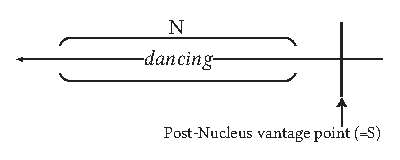
\includegraphics{figures/GrafikActivityCompletive.eps}
\caption{Perfective with an activity verb}
\label{FigurePerfectiveActivity}
\end{center}
\end{figure}

\begin{figure} 
\begin{center}
\caption{\label{FigurePerfectiveInchoative}Perfective with an inchoative verb}
\subfigure[Stative reading]{
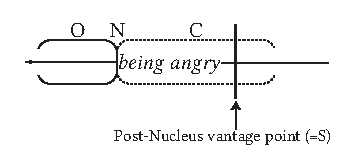
\includegraphics[width=0.47\textwidth]{figures/GrafikInchoativeStative.eps}}
\subfigure[Change-of-state reading]{
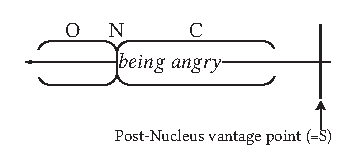
\includegraphics[width=0.47\textwidth]{figures/GrafikInchoativeChangeOfState.eps}}
\is{completion|)}
\end{center}
\end{figure}

 \newpage 
\subsubsection{Present perfective vs. anterior}\label{PRSPFVvsAnterior}
\is{aspect!anterior|(}It is opportune at this point to consider an alternative analysis of present perfective construction. At first glance, the Nyakyusa configuration \textit{ø}-\textsc{vb}-\textit{ile} resembles an \textit{anterior} or \textit{perfect}.\footnote{The term \textit{anterior}, as used by among others \citet{BybeePerkinsPaglucia1994}, is synonymous with the traditional \textit{perfect}, but has the advantage of not being easily confused with \textit{perfective}.} This is how it has been labelled in some of the previous accounts of Nyakyusa: \citet{SchumannK1899} speaks of a \lq\lq Perfectum'' and \citet{EndemannC1914} of a \lq\lq Perfekt''. Likewise, \citet{MwangokaNVoorhoeveJ1960b} use the label \lq\lq recent perfect''. The anterior (perfect) is also how this construction is in many cases conveniently translated into English. In fact, the Nyakyusa present perfective covers all of the sentences in \citeauthor{DahlOe1985}'s (\citeyear{DahlOe1985}) tense and aspect questionnaire that are identified as prototypical for the employment of the crosslinguistic category of anteriors.

An analysis as an anterior is also suggested by the criteria proposed in Nurse's pan-Bantu study of tense and aspect, in which he identifies the configuration \mbox{\textit{ø}-}\textsc{vb}\mbox{-\textit{ile}} as the most common marker of anteriors in his sample of Bantu languages \citep[156]{NurseD2008}. More importantly, \citet[95--99]{NurseD2008} proposes a number of criteria specific to the morphosyntactic make-up of Bantu languages in order to distinguish between anteriors on the one hand and near past perfectives on the other. Two of these criteria can readily be applied to Nyakyusa. The first one concerns the interaction of grammatical aspect with the aspectual potential of the lexical verb. Drawing on the concepts of consequent state and relevance, which are widely considered core components of anteriors, \citeauthor{NurseD2008} states:
\begin{quote}
For an action verb, for example, anterior represents a situation that is completed but relevant, whereas for a stative verb anterior represents the continuing state resulting from an action initiated in the past. \citep[73]{NurseD2008}
\end{quote}

\newpage 
As has been seen in \sectref{PresentPerfectiveIntroduction}, while a resultant state reading is indeed the default for the Nyakyusa present perfective with \isi{inchoative verbs} (Nurse’s statives), a dynamic change-of-state reading is also available. More example cases are given in the following. In (\ref{exInchoativeChangeOfStateOver}) the resultant state is explicitly cancelled for utterance time, leaving only the dynamic reading. In (\ref{exInchoativeChangeOfStateExistential}), the question is about a previous event of turning angry, not a present state.\footnote{See \sectref{MoSome} on the enclitic =\textit{mo}.} Lastly, in (\ref{exInchoativeChangeOfStateTemporalAdverb}) the event time adverbial phrase \lq last year' allows only for a change-of-state reading. While \lq to die' in English is often considered a punctual achievement (e.g. \citealt[54]{DowtyD1979}), its Nyakyusa equivalent \textit{fwa} is an inchoative verb\is{inchoative verbs} best translated as \lq to be moribund/die/be dead'; see \sectref{VerbalClassTransitionalAchievement}. Also note that lexical verbs which are non-inchoative but suggest the entry into a state do not depend upon a result persisting at utterance time, as with \textit{isa} \lq come' in (\ref{exPRSPFVsequence2}) below.

\begin{exe}
\ex \label{exInchoativeChangeOfStateOver}\gll ii-treni ly-ɪm-ile, lɪno li-kw-end-a kangɪ\\
5-train(<SWA) 5-stand/stop-\textsc{pfv} now 5-\textsc{prs}-walk/travel-\textsc{fv} again\\
\glt \lq The train stopped, but now it is moving again.' [ET]
\ex \label{exInchoativeChangeOfStateExistential} \gll a-kaleele=mo sikʊ baaba gw-ako?\\ 1-be(come)\_angry.\textsc{pfv}=some ever father(<SWA) 1-\textsc{poss.2sg}\\\glt `Has your father ever become angry?' [ET] %ist gecheckt <-lieber hier behalten, als 'weiteres BSP'
\ex \label{exInchoativeChangeOfStateTemporalAdverb} \gll a-fw-ile ɪ-ky-ɪnja ɪ-kɪ kɪ-kɪnd-ile\\
1-die-\textsc{pfv} \textsc{aug}-7-year \textsc{aug}-\textsc{prox.7} 7-pass-\textsc{pfv}\\
\glt `He died last year.' [ET]
\end{exe}

What is more, the present perfective does not feature a strong relevance component. Instead it is the default paradigm for relating recent non-progressive states-of-affairs. In doing so it can be freely used with sequential eventualities, which is a negative criterion for anteriors (\citealt[138]{DahlOe1985}; \citealt[54]{BybeePerkinsPaglucia1994}; \citealt[371]{LindstedtJ2000}). The following examples illustrate both points. In (\ref{exPRSPFVsequence1}) Tortoise asks his child for the whereabouts of a grindstone. Tortoise's child's answer consists of three clauses. In the first, the past perfective with inchoative \textit{kalala} \lq be(come) angry' refers to Mr. Monkey's previous state of mind, which has not only passed but is background information. In the two following clauses, the eventualities affecting the discourse topic (the grindstone) are summarized in the form of a minimal narrative using the present perfective. In (\ref{exPRSPFVsequence2}) a woman reports to her husband the recent happenings, again using two narrative clauses\is{clause types (Labov \& Waletzky)!narrative clause} with the present perfective.

\begin{exe}
\ex \label{exPRSPFVsequence1}
\gll mw-anangʊ, lʊ-lɪ koo=kʊʊgʊ ʊ-lw-ala lw-angʊ?\\
1-my\_child 11-\textsc{cop} \textsc{ref}.17=where \textsc{aug}-11-grindstone 11-\textsc{poss.1sg}\\
\glt `[Tortoise:] My child, where is my grindstone?'
\sn \gll aah, mwa=n-gambɪlɪ a-a-kaleele fiijo. \textbf{eeg}-\textbf{ile} ʊ-lw-ala lʊ-la, \textbf{a}-\textbf{taag}-\textbf{ile} m-mi-syanjʊ\\
 \textsc{interj} matronym=9-monkey 1-\textsc{pst}-be(come)\_angry.\textsc{pfv} \textsc{intens} 1.take-\textsc{pfv} \textsc{aug}-11-grindstone 11-\textsc{dist} 1-throw-\textsc{pfv} 18-4-bush\\
\glt \lq [Tortoise's child:] Aah, Mr. Monkey was very angry. He took that grindstone, he threw it into the bush.' [Monkey and Tortoise]
\ex \label{exPRSPFVsequence2} \gll \textbf{iis}-\textbf{ile}=\textbf{po} ʊ-mu-ndʊ jʊ-mo, a-a-sʊʊm-aga a-ma-beele. leelo \textbf{n}-\textbf{um̩}-\textbf{bʊʊl}-\textbf{ile} ʊkʊtɪ iis-e na=a-ma-jolo\\
1.come-\textsc{pfv}=16 \textsc{aug}-1-person 1-one 1-\textsc{pst}-beg-\textsc{ipfv} \textsc{aug}-6-breast\_milk now/but \textsc{1sg}-1-tell-\textsc{pfv} \textsc{comp} 1.come-\textsc{subj} \textsc{com}=\textsc{aug}-6-evening\\
\glt `Somebody came by, she was asking for breast milk. I told her to come back in the evening.' [Killer woman]
\end{exe} 

To sum up so far, the Nyakyusa present perfective neither necessarily brings about a persistent result, nor does it feature a strong relevance component. Now, recall from \sectref{TenseAspect} that \citeauthor{BotneRKershnerT2008} define tense in terms of inclusion and exclusion of the deictic locus. Being a present tense construction, not only does the vantage point evoked by the present perfective by default coincide with the time of speech, but the eventuality depicted is also situated within the same reference frame. Any notion of prevailing effects can thus be understood as a mere function of the eventuality being included within the here-and-now reality of the speech event, particularly when taking into consideration the opposition to its past tense\is{tense!past} counterpart \mbox{a(\textit{lɪ})-}\textsc{vb}\mbox{-\textit{ile}}. There is thus no need to assume any of the further components of meaning commonly assumed in the literature on anteriors such as the introduction of a \lq\lq perfect state'' (\citealt{MoensM1987}; \citealt{MoensMSteedmanM1988}), \lq\lq result state'' \citep{KampHReyleU1993} or a modal presupposition \citep{PortnerP2003};\footnote{Also note that these authors, in drawing on \citet{ReichenbachH1947}, take as a starting point the temporal ordering of an eventuality relative to a reference point (which for a present anterior equals time of speech), as in \citeauthor{ReichenbachH1947}'s famous formalisation \lq\lq E--R,S''. As seen in \sectref{PerfectivityCompletion}, the vantage point evoked rather follows the characteristic act (Nucleus)\is{phase!Nucleus phase} which may be followed by a resultant state phase (Coda).\is{phase!Coda phase}} see \citet{RitzM2012} for an overview of common theories of anteriors.

\largerpage
Nurse's second criterion concerns compound verb constructions. Anteriors, but not perfectives, should be found in these. The present perfective with \isi{inchoative verbs} can serve as the complement of the persistive aspect \isi{auxiliary} (\sectref{Persistive}),\is{aspect!persistive} which would speak in favour of a classification as an anterior. However, the same combinatory possibility also holds for the past perfective, which itself is most likely derived historically from a compound verb construction consisting of the \isi{copula} plus the present perfective (\sectref{PastPerfective}).

Furthermore, the notion of \lq still', as expressed through the persistive in Nyakyusa, is typically incompatible with anteriors (see \citealt{NedjalkovPJaxontovS1988} among others). To combine with `still' is instead said to be a hallmark of resultatives.\is{resultative} These are grammatical constructions that express a state brought about by a past situation. In this they differ from anteriors, which focus on the past situation itself (\citealt[134]{DahlOe1985}; \citealt[69]{BybeePerkinsPaglucia1994}). The Nyakyusa perfective in its stative reading asserts that the subject is in the resultant state of the act lexically encoded as the Nucleus, and thus comes closer to a \isi{resultative} than to an anterior. As seen in \sectref{PerfectivityCompletion} above, this resultative-like\is{aspect!resultative} reading falls out naturally from the analysis of \mbox{-\textit{ile}} as a marker of nuclear completion.\is{completion}\is{phase!Nucleus phase}

Lastly, consider the organization of the Nyakyusa TAM system. Within the present tense, the perfective contrasts primarily with the simple present.\is{simple present} While the perfective selects a time posterior to the right edge of the Nucleus phase,\is{phase!Nucleus phase} the simple present denotes the unfolding or future occurrence of a single eventuality. That is, it denotes a time before the endpoint of the Nucleus.\is{phase!Nucleus phase} In the past tense,\is{tense!past} the very same opposition is found between the past perfective -- which shows the same interaction with the lexical dimension -- and the past imperfective.\is{aspect!imperfective}\is{aspect!grammatical}

In sum, an analysis of the configuration \textit{ø}-\textsc{vb}-\textit{ile} as an anterior is contradicted by its semantics and distribution. Instead, its meaning and use, including any overlap with the crosslinguistic category of anterior, are readily explained by the aspectual notion of a post-Nucleus vantage point, together with the present tense \lq\lq denoting a primary, prevailing [\ldots] perspective'' \citep[153]{BotneRKershnerT2008}. What is more, postulating an analysis of \textit{ø}-\textsc{vb}-\textit{ile} as an anterior would preclude a compositional analysis of its past-marked counterpart \mbox{\textit{a}(\textit{lɪ})-}\textsc{vb}-\mbox{\textit{ile}}.\footnote{Unless both are analysed as anteriors, which would not only render this label vacuous, but is contradicted by the negative criteria of their compatibility with sequential events and persistive aspect.\is{aspect!persistive}} It would also miss the systematic parallel between the aspectual oppositions in the present and past tenses.
\is{aspect!anterior|)}
\subsubsection{Summary}
To sum up, the Nyakyusa present perfective depicts the \isi{completion} of an eventuality's Nucleus\is{phase!Nucleus phase} without dissociation to a distant reference frame. In this it forms part of a coherent grammatical system, centred around the notions of perfectivity as \isi{completion} of the Nucleus phase\is{phase!Nucleus phase} in the dimension of grammatical aspect,\is{aspect!grammatical} and association vs. dissociation in the dimension of tense.\is{tense}

Consistent with this analysis, in past tense \isi{narrative} discourse the present perfective is found in a few clearly determined environments: first, as a narrative present,\is{narrative present} where it provides information ancillary to the storyline and patterns with the \isi{simple present} and present copula;\is{copula} and second, with relative time reference in subordinate clauses.\is{subordinate clauses} These two kinds of uses are discussed separately in \sectref{PRSasNonPST}. Lastly, it features in the coda section\is{section!coda} of some narratives (\ref{PRSPFVCodaNarration}), where it refers to the speaker-now and is again in predictable alternation with the other present-tense paradigms.

\begin{exe}
\ex \label{PRSPFVCodaNarration} \gll a-ka-pango ka-mal-iike\\
\textsc{aug}-12-story 12-finish-\textsc{neut}.\textsc{pfv}\\
\glt \lq The story is over.' [Monster with Guitar]
\end{exe}
\is{tense!present|)}\is{aspect!perfective|)}

\subsection{Negative present perfective}\label{NEGPresentPerfective}
\is{tense!present|(}\is{negative|(}
The negative counterpart to the present perfective\is{aspect!perfective} consists of the negative post-initial prefix \textit{ka}- and the default final vowel -\textit{a}.

\begin{exe}
\ex \textit{tʊkajoba} \lq we have not spoken'
\end{exe}
With inchoative verbs,\is{inchoative verbs} this construction typically negates the resultant state (\ref{NegPrsPfv1}), while with non-inchoatives, the eventuality is typically understood not to have occurred (\ref{NegPrsPfv2}).

\begin{exe}
\ex \label{NegPrsPfv1}\gll \textbf{ba}-\textbf{k}-\textbf{ii}-\textbf{gan}-\textbf{a} ʊ-kʊ-bomb-el-a ɪ-fy-ombo ɪ-fy-a kw-asim-a kʊ-ba-palamani\\
2-\textsc{neg}-\textsc{refl}-like-\textsc{fv} \textsc{aug}-15-work-\textsc{appl}-\textsc{fv} \textsc{aug}-8-tool \textsc{aug}-8-\textsc{assoc} 15-borrow-\textsc{fv} 17-2-neighbour\\
\glt \lq They do not like to work with tools borrowed from neighbours' [Types of tools in the home] %inchoative
\ex  \label{NegPrsPfv2}\gll mma, \textbf{a}-\textbf{ka}-\textbf{job}-\textbf{a} bo ʊ-lʊ. a-t-ile \textup{\lq\lq}kalʊlʊ ʊ-jʊ n-heesya gw-ɪtʊ\textup{''}\\
no, 1-\textsc{neg}-speak-\textsc{fv} as \textsc{aug}-\textsc{prox.11} 1-say-\textsc{pfv} \phantom{\lq\lq}hare(1) \textsc{aug}-\textsc{prox.1} 1-foreigner 1-\textsc{poss.1pl}\\
\glt \lq No, he didn't speak like that. He said \lq\lq This hare's our guest.''' [Saliki and Hare]
%non-inchoative
\end{exe}
Examples such as (\ref{exImperfectiveParadox1}, \ref{exImperfectiveParadox2}) constitute a variation on \citeauthor{DowtyD1979}'s (\citeyear{DowtyD1979}) \lq\lq imperfective paradox''.\is{aspect!imperfective} These were judged redundant but not contradictory. This suggests that what is actually negated is the \isi{completion} of the Nucleus phase.\is{phase!Nucleus phase}

\begin{exe}
\ex \label{exImperfectiveParadox1} \gll a-ka-fik-a, leelo a-lɪ pa-kʊ-fik-a\\
1-\textsc{neg}-arrive-\textsc{fv} now/but 1-\textsc{cop} 16-15-arrive-\textsc{fv}\\
\glt \lq He has not arrived (yet), but he is arriving.' [ET]
\ex \label{exImperfectiveParadox2} \gll a-ka-kalal-a, leelo a-lɪ pa-kʊ-kalal-a\\
1-\textsc{neg}-be(come)\_angry-\textsc{fv} now/but 1-\textsc{cop} 16-15-be(come)\_angry-\textsc{fv}\\
\glt \lq He is not angry (yet), but he is about to get angry.' [ET]
\end{exe}
\is{tense!present|)}\is{negative|)}
\subsection{Past perfective}\label{PastPerfective}
\is{tense!past|(}\is{aspect!perfective|(}
\subsubsection{Formal makeup}
The past perfective consists of a prefix \textit{a}- and the suffix -\textit{ile} (\ref{exPSTPFValiConsonantInitial}); see \sectref{Imbrication} on the allomorphs of -\textit{ile}. Preceding a vowel, i.e. in vowel-initial stems (\ref{exPSTPFValiVowelInitial}) or the reflexive object marker (\ref{exPSTPFValiReflexive}), the prefix of the past perfective has the allomorph \textit{alɪ}-. The usual rules of pre-stem vowel contact apply; see \sectref{HiatusSolution}.

\begin{exe}
\ex \label{exPSTPFValiConsonantInitial}
\begin{tabbing}
\textit{twaliikeetile}x\=(\degree tʊ-alɪ-i-keet-ile)x\=\kill
\textit{twabombile}\>(\degree tʊ-a-bomb-ile)\>`we worked'\\
\textit{twakeetile}\>(\degree tʊ-a-keet-ile)\>`we watched'
\end{tabbing}
\ex \label{exPSTPFValiVowelInitial}
\begin{tabbing}
\textit{twaliikeetile}x\=(\degree tʊ-alɪ-i-keet-ile)x\=\kill
\textit{twaliisile}\>(\degree tʊ-alɪ-is-ile)\>`we came'\\
\textit{twalyɪmile}\>(\degree tʊ-alɪ-ɪm-ile)\>`we stopped'\\
\textit{twalyegile}\>(\degree tʊ-alɪ-eg-ile)\>`we took'\\
\textit{twalyagile}\>(\degree tʊ-alɪ-ag-ile)\>`we found'\\
\textit{twalyogile}\>(\degree tʊ-alɪ-og-ile)\>`we bathed'\\
\textit{twalyʊmile}\>(\degree tʊ-alɪ-ʊm-ile)\>`we dried'
\end{tabbing}
\ex
\label{exPSTPFValiReflexive}
\begin{tabbing}
\textit{twaliikeetile}x\=(\degree tʊ-alɪ-i-keet-ile)x\=\kill
\textit{twaliikeetile}\>(\degree tʊ-alɪ-i-keet-ile)\>`we looked at ourselves'\\
\textit{twaliipakile}\>(\degree tʊ-alɪ-i-pak-ile)\>`we painted ourselves' 
\end{tabbing}
\end{exe}
The same allomorph \textit{alɪ}- also surfaces preceding the object markers\is{object marker} of the first person singular (\ref{exPSTPFValiOM1SG}) and noun class 1 (\ref{exPSTPFValiOMNCL1}), regardless of their respective allomorphs.\footnote{See \sectref{sectionParticipantOM}, \ref{sectionNCLOM} on the morphophonemics of these prefixes.}

\pagebreak
\begin{exe}
\ex\label{exPSTPFValiOM1SG}
\begin{tabbing}
\textit{mwalɪndaagile}x\=(\degree mu-alɪ-ny-taag-ile)x\=\kill
\textit{mwalɪndaagile}\>(\degree mu-alɪ-ny-taag-ile)\>`you (pl.) threw me'\\
\textit{mwalɪmbʊʊlile}\>(\degree mu-alɪ-ny-bʊʊl-ile)\>`you (pl.) told me'\\
\textit{mwalɪɪmetile}\>(\degree mu-alɪ-ny-met-ile)\>`you (pl.) shaved me'\\
\textit{mwalɪɪsalile}\>(\degree mu-alɪ-ny-sal-ile)\>`you (pl.) chose me'\\
\textit{mwalɪɪnyaagile}\>(\degree mu-alɪ-ny-ag-ile)\>`you (pl.) found me'
\end{tabbing}
\ex\label{exPSTPFValiOMNCL1}
\begin{tabbing}
\textit{twalɪmmwagile}x\=(\degree tʊ-alɪ-mu-bʊʊl-ile)x\=\kill%sinnnlose Zeile, fuer Tabulatoren
\textit{twalɪntaagile}\>(\degree tʊ-alɪ-mu-taag-ile)\>`we threw him/her'\\
\textit{twalɪm̩bʊʊlile}\>(\degree tʊ-alɪ-mu-bʊʊl-ile)\>`we told him/her'\\
\textit{twalɪmmetile}\>(\degree tʊ-alɪ-mu-met-ile)\>`we shaved him/her'\\
\textit{twalɪnsalile}\>(\degree tʊ-alɪ-mu-sal-ile)\>`we chose him/her'\\
\textit{twalɪmmwagile}\>(\degree tʊ-alɪ-mu-ag-ile)\>`we found him/her'\\ 
\textit{twalɪmmootile}\>(\degree tʊ-alɪ-mu-ot-ile)\>`we invited him/her'
\end{tabbing}
\end{exe}

The sequence /lɪ/ indicates that diachronically the longer form of the prefix is derived from a serial construction involving the \isi{copula} \textit{lɪ} (see \citealt{BotneR1986}). From a synchronic perspective, this allomorphy finds a functional explanation: due to the rules of vowel coalescence (\sectref{HiatusSolution}),\is{vowels!hiatus solution} a prefix \textit{a}- would assimilate to the vowel of vowel-initial stems and the \isi{reflexive} prefix, resulting in forms homophonous with the present perfective. Similarly, any vowel preceding the first person singular object prefix surfaces as long\is{vowels!length} (\sectref{sectionParticipantOM}), while any vowel preceding the class 1 object prefix surfaces as short\is{vowels!length} (\sectref{sectionNCLOM}). Again, without the alternation \textit{a}-/\textit{alɪ}- this would result in formal identity of the present and past perfective with subjects of \isi{noun classes} 1, 2, 6, 12 and 16. Note that classes 1 and 2 include all human beings. Thus the alternation between \textit{a}- and \textit{alɪ}- serves to avoid a high degree of ambiguity.\footnote{Interestingly, where Nyakyusa has \textit{ø}-\textsc{vb}-\textit{ile} vs. \textit{a(lɪ)}-\textsc{vb}-\textit{ile}, the \ili{Ngonde} variety described by \citet[76f]{KishindoP1999} has an opposition between \textit{a}-\textsc{vb}-\textit{ile} and \textit{ali}-\textsc{vb}-\textit{ile}.}

\subsubsection{Overview of meaning}\label{PastPerfectiveOverviewMeaning}
The past perfective construes a state-of-affairs as situated in the conceptual past (i.e. past D-domain in \citeauthor{BotneRKershnerT2008}'s framework; see \sectref{Tense}) with its Nucleus phase\is{phase!Nucleus phase} completed.\is{completion} The aspectual notion of \isi{completion} is discussed in more detail in \sectref{PerfectivityCompletion}. As (\ref{exPSTPFValiOM1SG}, \ref{exPSTPFValiOMNCL1}) show, with non-inchoative verbs this gives a typical posterior reading. With inchoative verbs,\is{inchoative verbs} the default reading is one of a state holding at some contextually defined past moment:

\begin{exe}
\ex \gll a-a-kaleele\\
1-\textsc{pst}-be(come)\_angry.\textsc{pfv}\\
\glt (Default reading:) \lq S/he was angry.' [ET]
\end{exe}

However, a posterior, holistic perspective is also possible with inchoative verbs. In the opening of a \isi{narrative} given in (\ref{exPSTPFVinchoativePosterior1}), the past perfective with the inchoative verb \textit{lambalala} \lq lie down, sleep' depicts the eventuality as a whole, rather than the state of being asleep at a certain point in time. The same holds for the inchoative verb\is{inchoative verbs} \textit{gona} \lq rest, sleep' in (\ref{exPSTPFVinchoativePosterior2}).

\begin{exe}
\ex \label{exPSTPFVinchoativePosterior1}\gll po leelo ɪ-n-galamu j-aa-lɪ m-bine. \textbf{j}-\textbf{aa}-\textbf{lambaleele} a-ma-sikʊ ma-tatʊ n-nyumba\\
then now/but \textsc{aug}-9-lion 9-\textsc{pst}-\textsc{cop} 9-ill 9-\textsc{pst}-lie\_down.\textsc{pfv} \textsc{aug}-6-day 6-three 18-house(9)\\
\glt \lq Lion was ill. He slept for three days in his house.' [Lion and Tortoise]

\ex \label{exPSTPFVinchoativePosterior2}
\gll bo a-fik-ile kʊ-ka-aja \textbf{a}-\textbf{a}-\textbf{gon}-\textbf{ile}. n=ʊ-lʊ-bʊnjʊ a-lɪnkʊ-bʊʊk-a m-ma-tengele\\
as 1-arrive-\textsc{pfv} 17-12-homestead 1-\textsc{pst}-rest-\textsc{pfv} \textsc{com}=\textsc{aug}-11-morning 1-\textsc{narr}-go-\textsc{fv} 18-6-bush\\
\glt \lq When she arrived home, she slept. In the morning she went into the bush.' [Mfyage turns into a lion] %es sei denn, noch besseres bsp gehalten
\end{exe}

Note that the past perfective by itself does not denote sequential events. Consider the following plot summary of a story, which was given subsequent to the \isi{narrative} itself; Hare's running alone, mentioned for the first time in (\ref{exHareTugutuSummarySentences1and2}), only takes place after Tugutu's preparations (\ref{exHareTugutuSummarySentence4}, \ref{exHareTugutuSummarySentence5}). The flowchart in \figref{FigureRelativeOrderHareTugutuSummary} illustrates the relative order of events. The shunt to the right symbolizes that the \isi{negative} verb in (\ref{exHareTugutuSummarySentence3})  remains outside the sequence as a function of its negative polarity.

\begin{exe}
\ex \label{exHareTugutuSummary} \begin{xlist}
\ex\label{exHareTugutuSummarySentences1and2}\gll a-a-bop-ile mw-ene, a-a-bop-ile mw-ene kalʊlʊ\\
1-\textsc{pst}-run-\textsc{pfv} 1-self 1-\textsc{pst}-run-\textsc{pfv} 1-self hare(1)\\
\glt `He ran alone, Hare ran alone.'
\ex\label{exHareTugutuSummarySentence3}\gll mwa=n-dugutu a-ka-a-bop-ile=po\\
matronym=9-type\_of\_bird 1-\textsc{neg}-\textsc{pst}-run-\textsc{pfv}=\textsc{part}\\
\glt `Mr. Tugutu did not run at all.'
\ex\label{exHareTugutuSummarySentence4}\gll a-a-ba-paal-ile a-ba-nine\\
1-\textsc{pst}-2-invite-\textsc{pfv} \textsc{aug}-2-colleague\\
\glt \lq He had gathered companions.'
\ex\label{exHareTugutuSummarySentence5}\gll bo a-ba a-a-ba-bɪɪk-ile ʊ-kʊ-tɪ maelɪ jɪ-mo, maelɪ jɪ-mo, maelɪ jɪ-mo\\
\textsc{ref.2} \textsc{aug}-\textsc{prox.2} 1-\textsc{pst}-2-put-\textsc{pfv} \textsc{aug}-15-say mile(9)(<EN) 9-one mile(9) 9-one mile(9) 9-one\\
\glt \lq Those are the ones he placed, like one mile, one mile, one mile.'%gutes bsp cleft
\ex\label{exHareTugutuSummarySentence6}\gll po kalʊlʊ a-a-bop-ile mw-ene\\
then hare(1) 1-\textsc{pst}-run-\textsc{pfv} 1-self\\
\glt \lq So Hare ran alone.' [Hare and Tugutu]
\end{xlist}
\end{exe}

\begin{figure}[hbt]
\begin{center}
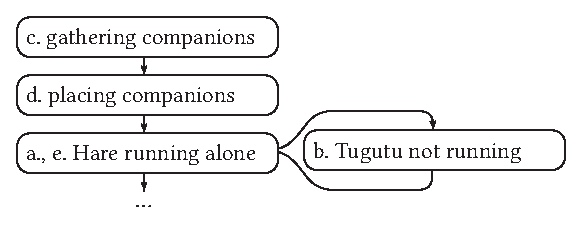
\includegraphics{figures/GrafikRelativeOrderHareTugutuPFV.eps}
\caption{Relative event order of (\ref{exHareTugutuSummary})}
\label{FigureRelativeOrderHareTugutuSummary}
\end{center}
\end{figure}
 
\subsubsection{The past perfective in narrative discourse}
\label{PastPerfectiveNarrative}\is{narrative|(}
\paragraph{Introduction}
While in many languages a perfective form is the principle paradigm for relating the storyline in narrative discourse (see i.a. \citealt{HopperP1979}; \citealt{FleischmanS1990}), this does not hold for Nyakyusa.\footnote{For a recent discussion of the relationship between TMA constructions and narrating in African languages see \citet{PayneDLShirtzS2015}.} As discussed in \sectref{NarrativeMarkersLicensingDependency}, none of the narrative texts in the corpus exclusively features the past perfective  in the recollection of storyline eventualities. Instead, Nyakyusa possesses two dedicated \isi{narrative markers} -- see \sectref{NarrativeMarkersApproximation} for an introduction -- which are employed in a collaborative manner together with the past perfective to fulfil this function. 

As was observed in the discussion of (\ref{exHareTugutuSummary}) above, the past perfective may be used with sequential events, but does not inherently encode any chronological ordering. Further, what is construed with the past perfective has an independent existence in discourse, quite contrary to the \isi{narrative tense} and subsecutive,\is{subsecutive} which are pragmatically dependent and thus embedded in a situation established by other means, usually through the use of a preceding past tense verb (\sectref{NarrativeMarkersLicensingDependency}). A series of mere past perfectives, such as the plot summary in (\ref{exHareTugutuSummary}) above, thus results in a loose enumeration of discrete events rather than forming a coherent narrative discourse of its own.

 
In the following, the usage of the past perfective in Nyakyusa narrative discourse will be outlined. In order to identify patterns of usage, it is necessary to first take a look at the typical composition of Nyakyusa narratives\is{narrative} (\sectref{PastPFVNarrativeDiscourseOpenings}--\ref{PastPFVNarrativeDiscourseSupportive}). Considering a set of occurrences not readily explained by notions of textual macro-structure (\sectref{PastPFVNarrativeDiscourseOtherDiscontinuities}), it will then be shown that the various uses of the past perfective in \isi{narrative} discourse form part of a larger coherent pattern of tense usage, whose common denominator is the notion of \isi{thematic continuity} (\sectref{PastPFVNarrativeDiscourseSummary}). The following analysis is based mainly on the oral narratives\is{narrative} in the corpus, but some additional examples were taken from written texts.

  
\paragraph{Opening a narrative}\label{PastPFVNarrativeDiscourseOpenings}
A narrative in Nyakyusa typically opens with an orientation section\is{section!orientation} of varying length. By definition  -- see \sectref{ToolsNarrativeAnalysis} -- the orientation section\is{section!orientation} depicts states-of-affairs that hold throughout the whole text and orient the listener in respect to the setting. In the expected division of labour with the other past tense paradigms, the past perfective is used here with inchoative verbs,\is{inchoative verbs} giving a stative reading (\ref{exPSTPFVOrientationSectionInchoative}), as well as with non-inchoatives, which have a pluperfect reading (\ref{exPSTPFVOrientationSectionPluPerfect}).

\begin{exe}
\ex \label{exPSTPFVOrientationSectionInchoative}
\gll a-a-li=ko kalʊlʊ n=ɪɪ-fubu. \textbf{ba}-\textbf{a}-\textbf{many}-\textbf{eene} fiijo. kangɪ b-angal-aga pamopeene ʊ-bʊ-sikʊ b-oosa\\
1-\textsc{pst}-\textsc{cop}=17 hare(1) \textsc{com}=\textsc{aug}-hippo(9) 2-\textsc{pst}-know-\textsc{recp.pfv} \textsc{intens} again 2-\textsc{pst}.be\_well-\textsc{ipfv} together \textsc{aug}-14-time 14-all\\
\glt \lq Once upon a time, Hare and Hippo were very much friends. And they used to be together the whole time.' [Hare and Hippo]

\ex \label{exPSTPFVOrientationSectionPluPerfect}
\gll ijolo ky-a-li=ko ɪ-ky-amba. pa-mwanya pa-ky-amba pa-a-lɪ pa-tengaamu itolo. \textbf{ba}-\textbf{a}-\textbf{jeng}-\textbf{ile}=\textbf{po} a-ba-ndʊ ba-tatʊ\\
old\_times 7-\textsc{pst}-\textsc{cop}=17 \textsc{aug}-7-mountain 16-high 16-7-mountain 16-\textsc{pst}-\textsc{cop} 16-peaceful just 2-\textsc{pst}-build-\textsc{pfv}=16 \textsc{aug}-2-person 2-three\\
\glt \lq Long ago there was a mountain. On top of the mountain it was all peaceful. Three people had built there.' [Selfishness kills]
\end{exe}%xxx vokallänge nochmal checken tenga(a?)mu

Following the orientation section,\is{section!orientation} one commonly finds a verb in one of the past tense paradigms that sets the stage for the first episode. In cases where there is no orientation section,\is{section!orientation} this constitutes the opening of the text. For an example of the past perfective in this environment, see (\ref{exNarrBeginningPlotUnequalNarr}) on p.\nobreakspace\pageref{exNarrBeginningPlotUnequalNarr}.

\paragraph{Textual boundaries}\label{PastPFVNarrativeDiscourseBoundaries}
In longer narratives, subsequent major units are commonly also delimited by one or more past tense verbs. This often implies a shift away from one of the narrative markers.\is{narrative markers} These verbs depict the state-of-affairs out of which the following course of events develops. Again, the past perfective, imperfective\is{aspect!imperfective} and \isi{copula} pattern together, depending on the aspectual profile\is{aspect!grammatical} of the state-of-affairs and the verb's Aristotelian aspect.\is{aspect!Aristotelian}

It is important to note at this point that the notions of boundary marking and staging operate within the textual component.\is{component of meaning!textual} An event that forms part of the semantic storyline may additionally be construed as the setting of a unit within the text if it depicts the circumstances under which following eventualities take place \citep{PayneD1992}. By virtue of its aspectual semantics,\is{aspect!grammatical} it is the past perfective that is employed in these cases. Further, it is typically not every episode within longer texts that starts out with a past tense. The following examples will illustrate both points.

In the text \lq\lq Monkey and Tortoise'', lazy but witty Tortoise sends his child to Monkey's to get food, pretending to buy it on credit. After obtaining the food, little Tortoise returns home. They enjoy their meals and never make the agreed payment (\ref{exMonkeyTortoiseFirstNoPaying}). Clause (\ref{exMonkeyTortoiseSentence1}) is the last one in the food-obtaining episode. The following clauses (\ref{exMonkeyTortoiseSentence2}--\ref{exMonkeyTortoiseSentences6and7}) are all marked for past tense and group together to describe a major discontinuity in action and time. Of these, (\ref{exMonkeyTortoiseSentences4and5}, \ref{exMonkeyTortoiseSentences6and7}), by virtue of the states-of-affairs they depict, as well as the fact that they include two negatives,\is{negative} give information that diverges from the main storyline. The eating in (\ref{exMonkeyTortoiseSentence2}), however, is no less eventive than the preceding walk home. Nevertheless, it is construed as part of the upcoming episode's setting.

\begin{exe}
\ex \label{exMonkeyTortoiseFirstNoPaying} \begin{xlist}
\ex \label{exMonkeyTortoiseSentence1} \gll po mw-ene jʊ-la gw-a kajamba a-lɪnkʊ-bʊʊk-a kʊ-ka-aja n=ɪ-fi-ndʊ fi-la\\
then 1-self 1-\textsc{dist} 1-\textsc{assoc} tortoise(1) 1-\textsc{narr}-go-\textsc{fv} 17-12-homestead \textsc{com}=\textsc{aug}-8-food 8-\textsc{dist}\\
\glt \lq Tortoise's child went home with that food.'
\ex \label{exMonkeyTortoiseSentence2}
\gll po n=ʊ-gwise po \textbf{ba}-\textbf{a}-\textbf{l}-\textbf{iile}\\
then \textsc{com}=\textsc{aug}-his\_father(1) then 2-\textsc{pst}-eat-\textsc{pfv}\\
\glt \lq  He and his father ate.'
\ex \label{exMonkeyTortoiseSentence3}
\gll po ba-a-hobwike fiijo a-ma-sikʊ ma-bɪlɪ\\
then 2-\textsc{pst}-be(come)\_happy.\textsc{pfv} \textsc{intens} \textsc{aug}-6-day 6-two\\
\glt \lq They were very happy for two days.'

\ex \label{exMonkeyTortoiseSentences4and5} \gll leelo bo gɪ-kɪnd-ile ɪ-mi-lʊngʊ mi-bɪlɪ, kajamba a-ka-a-buj-iisye. a-ka-a-bʊʊk-ile kw-a mwa=n-gambɪlɪ kʊ-kʊ-bɪɪk-a ɪɪ-heela\\
now/but as 4-pass-\textsc{pfv} \textsc{aug}-4-week 4-two tortoise(1) 1-\textsc{neg}-\textsc{pst}-return-\textsc{caus.pfv} 1-\textsc{neg}-\textsc{pst}-go-\textsc{pfv} 17-\textsc{assoc} matronym=9-monkey 17-15-put-\textsc{fv} \textsc{aug}-money(9)\\
\glt \lq When two weeks passed, Tortoise had not paid. ‎‎He had not gone to Monkey's to hand over the money.'

\ex  \label{exMonkeyTortoiseSentences6and7} \gll gw-a-kɪnd-ile ʊ-n̩-dʊngʊ gʊ-mo. gy-a-kɪnd-ile mi-bɪlɪ na=ka-mo n=ʊ-kʊ-bʊʊk-a kʊ-kʊ-bɪɪk-a\\
3-\textsc{pst}-pass-\textsc{pfv} \textsc{aug}-3-week 3-one 4-\textsc{pst}-pass-\textsc{pfv} 4-two \textsc{com}=12-one \textsc{com}=\textsc{aug}-15-go-\textsc{fv} 17-15-put-\textsc{fv}\\
\glt\lq One week passed. Two weeks passed, not once going to hand it over.'

\ex \label{exMonkeyTortoiseSentence8} \gll po mwa=n-gambɪlɪ a-a-tɪ \textup{\lq\lq}hee. po m-bʊʊk-e kw-a kajamba kʊ-kʊ-mel-a ɪɪ-heela sy-angʊ\textup{''}\\
as matronym=9-monkey 1-\textsc{subsec}-say \phantom{\lq\lq}\textsc{interj} then \textsc{1sg}-go-\textsc{subj} 17-\textsc{assoc} tortoise(1) 17-15-claim-\textsc{fv} \textsc{aug}-money(10) 10-\textsc{poss.1sg}\\
\glt \lq Then Monkey said \lq\lq Hee. ‎‎I shall go to Tortoise to demand my money.''{}'
\ex \label{exMonkeyTortoiseSentence9} \gll po a-lɪnkw-end-a, a-lɪnkw-end-a, a-lɪnkw-end-a\\
then 1-\textsc{narr}-walk/travel-\textsc{fv} 1-\textsc{narr}-walk/travel-\textsc{fv} 1-\textsc{narr}-walk/travel-\textsc{fv}\\
\glt \lq He walked and walked and walked.' [Monkey and Tortoise]
\end{xlist}
\end{exe}

With (\ref{exMonkeyTortoiseSentence8}, \ref{exMonkeyTortoiseSentence9}) the storyline continues. Tortoise makes an excuse and Monkey gives up on claiming his money that day. This episode is narrated entirely using the \isi{narrative markers} (plus one token of a narrative present).\is{narrative present} Now, after two more weeks, Monkey returns to Tortoise's only to hear another excuse and to go home again without his money. This episode, whose main events essentially repeat those of the preceding one, is not further delimited by a shift to the past tense (\ref{exMonkeyTortoiseNoStaging}).

\largerpage[2]
\begin{exe}
\ex \label{exMonkeyTortoiseNoStaging}
\begin{xlist}
\ex \label{exMonkeyTortoiseNoStagingSentence1} \gll kangɪ po bo gɪ-kɪnd-ile ɪ-mi-lʊngʊ mi-bɪlɪ, kangɪ \textbf{a}-\textbf{lɪnkʊ}-\textbf{buj}-\textbf{a} kw-a kajamba\\
again then as 4-pass-\textsc{pfv} \textsc{aug}-4-week 4-two again 1-\textsc{narr}-return-\textsc{fv} 17-\textsc{assoc} tortoise(1)\\
\glt \lq When two weeks had passed, he returned again to Tortoise's.'

\ex \gll bo i-kʊ-fik-a i-kʊ-mmw-ani-a ʊ-mw-anaake \lq\lq a-li=po ʊ-gʊʊso a-pa?''\\
as 1-\textsc{prs}-arrive-\textsc{fv} 1-\textsc{prs}-1-ask-\textsc{fv} \textsc{aug}-1-his\_child \phantom{\lq\lq}1-\textsc{cop}=16 \textsc{aug}-your\_father \textsc{aug}-\textsc{prox.16}\\
\glt \lq As he was arriving he asks his (Tortoise's) child \lq\lq Is your father here?''{}' [Monkey and Tortoise]
\end{xlist}
\end{exe}

In contrast, the next episode does start with a shift to the past tense (\ref{exMonkeyTortoiseStaging}). Note how the content of the first two clauses of this episode (\ref{exMonkeyTortoiseStagingSentence1}, \ref{exMonkeyTortoiseStagingSentence2}) mostly parallels the first clause of the preceding episode (\ref{exMonkeyTortoiseNoStagingSentence1}). The use of the past perfective instead of the \isi{narrative tense} coincides with a change in Monkey's attitude. This entails an important shift in the development of events. Instead of continuing the routine of the preceding two episodes, Tortoise finds himself needing to resort to a more elaborate trick to get away without paying his debts.
\begin{exe}
\ex\label{exMonkeyTortoiseStaging} 
\begin{xlist}
\ex \label{exMonkeyTortoiseStagingSentence1} \gll ii-sikʊ lɪ-lɪ-ngɪ po \textbf{a}-\textbf{al}-\textbf{iis}-\textbf{ile} mwa=n-gambɪlɪ\\
5-day 5-5-other then 1-\textsc{pst}-come-\textsc{pfv} matronym=9-monkey\\
\glt \lq Another day Mr. Monkey came.'
\ex \label{exMonkeyTortoiseStagingSentence2} \gll \textbf{a}-\textbf{al}-\textbf{iis}-\textbf{ile} n=ɪ-ly-ojo\\
1-\textsc{pst}-come-\textsc{pfv} \textsc{com}=\textsc{aug}-5-anger\\
\glt \lq He came with anger.'
\ex \gll \textup{\lq\lq}lɪlɪno kʊ-m-b-a=ko ɪɪ-heela j-angʊ, kʊ-m-b-a=ko ɪɪ-heela j-angʊ\textup{''} i-kʊ-job-a mu-n-jɪla\\
\phantom{\lq\lq}now/today \textsc{2sg.prs}-\textsc{1sg}-give-\textsc{fv}=17 \textsc{aug}-money(9) 9-\textsc{poss.1sg} \textsc{2sg.prs}-\textsc{1sg}-give-\textsc{fv}=17 \textsc{aug}-money(9) 9-\textsc{poss.1sg} 1-\textsc{prs}-speak-\textsc{fv} 18-9-path\\
\glt \lq\lq \lq Today you're giving me my money, you're giving me my money'', he is saying on his way.'
\ex\gll a-lɪnkw-a kʊ-fik-a pa-a kajamba\\
1-\textsc{narr}-go.\textsc{fv} 15-arrive-\textsc{fv} 16-\textsc{assoc} tortoise(1)\\
\glt \lq He arrived at Tortoise's.' [Monkey and Tortoise]
\end{xlist}
\end{exe}

\paragraph{Further supportive material}
\label{PastPFVNarrativeDiscourseSupportive}
The storyline may be sprinkled with occasional supportive information in the past tense, be it the past perfective, past imperfective\is{aspect!imperfective} or the past copula,\is{copula} or a \isi{narrative present} (see \sectref{NarrativePresent} on the latter). This may consist of embedded orientations, that is, states-of-affairs that hold throughout all or parts of the text. The past perfective is therefore used with inchoative verbs.\is{inchoative verbs} This is common with verbs depicting psychological states, as illustrated in (\ref{exPstPfvSupportiveInchoativeSentences2}). Note that with most \isi{inchoative verbs} the past perfective is the only paradigm that can denote the resultant state and not merely the change-of-state. 
\newpage
\begin{exe}
\ex Context: Monkey is waiting for Tortoise.

\begin{xlist}
\ex \gll a-a-j-ile kʊ-buj-a. \textup{\lq\lq}Hahaha mwa=n-gambɪlɪ ʊ-li=po. gw-is-ile, pole! n-gʊ-p-a lɪlɪno ɪɪ-heela sy-ako\textup{''}\\
1-\textsc{pst}-go-\textsc{pfv} 15-return-\textsc{fv} \phantom{\lq\lq}\textsc{interj} matronym=9-monkey \textsc{2sg}-\textsc{cop}=16 \textsc{2sg}-come-\textsc{pfv} sorry(<SWA) \textsc{1sg}-\textsc{prs}-give-\textsc{fv} now/today \textsc{aug}-money(10) 10-\textsc{poss.2sg}\\
\glt \lq He [Tortoise] went and returned. \lq\lq Hahaha, Mr. Monkey, you are here! You have come, sorry! I'm giving you your money now.''
\ex \label{exPstPfvSupportiveInchoativeSentences2}
 \gll po mwa=n-gambɪlɪ \textbf{a}-\textbf{a}-\textbf{hobwike} \textup{\lq\lq}haa \textup{(clapping hands)} mma po kʊ-m-b-a ahahaa\textup{''}\\
then matronym=9-monkey 1-\textsc{pst}-be(come)\_happy.\textsc{pfv}
\phantom{\lq\lq}\textsc{interj} {} no then \textsc{2sg.prs}-\textsc{1sg}-give-\textsc{fv} \textsc{interj}\\
\glt \lq Mr. Monkey was happy \lq\lq Haa (clapping hands), you are giving me [my money], ahahaa.'' [Monkey and Tortoise]
\end{xlist}
\end{exe}

The past perfective is also used for flashbacks. It is the only verbal paradigm attested in the case of flashbacks.

\begin{exe}
\ex Context: Tortoise's child and Monkey are waiting for Tortoise.
\begin{xlist}
\ex \gll ba-lɪnkʊ-m̩-bon-a bo a-fum-ile bo kʊ-la\\
2-\textsc{narr}-1-see-\textsc{fv} as 1-come\_from-\textsc{pfv} as 17-\textsc{dist}\\
\glt \lq They saw him [Tortoise] as he came from over there.' 

\ex \gll ʊ-tɪ \textbf{ba}-\textbf{alɪ}-\textbf{n}-\textbf{taag}-\textbf{ile} mu-m-mi-syanjʊ\\
\textsc{2sg}-say.\textsc{subj} 2-\textsc{pst}-1-throw-\textsc{pfv} 18-18-4-bush\\
\glt \lq Do you know, they had thrown him into the bush.'

\ex \gll po \textbf{a}-\textbf{a}-\textbf{j}-\textbf{ile} kw-end-a kʊ-la\\
then 1-\textsc{pst}-go-\textsc{pfv} 15-walk/travel-\textsc{fv} 17-\textsc{dist}\\
\glt \lq He had (gone and) had a walk there.'

\ex \gll \textbf{a}-\textbf{a}-\textbf{j}-\textbf{ile} kʊ-buj-a\\
1-\textsc{pst}-go-\textsc{pfv} 17-return-\textsc{fv}\\
\glt \lq He had gone and returned.' [Monkey and Tortoise]
\end{xlist}
\end{exe}

\paragraph{Further storyline events} \label{PastPFVNarrativeDiscourseOtherDiscontinuities}
As has been discussed thus far, the past perfective is frequently employed -- together with the other past tense paradigms -- in narrative discourse for setting the stage at major episode boundaries and for providing information ancillary to the storyline. In addition, it is commonly found in relating more storyline events, where its employment vis-à-vis the dedicated \isi{narrative markers} is not readily explained by the patterns described above. A closer examination shows that in these cases it normally depicts eventualities that are unpredictable, pivotal for the development of the plot and/or constitute a major change in the roles of participants.\footnote{\citet[8]{JonesLBJonesLK1979} define pivotal events as \lq\lq very crucial or significant events of a narrative [\ldots] when collected together, they form a high-level summary or abstract of the story''. This definition is reflected in \citet[90]{TomlinR1985} and \citet[5]{LongacreR1990}.} In \sectref{PastPFVNarrativeDiscourseSummary} below it will be shown that all these uses of the past perfective form part of one coherent pattern of employment of the past tense paradigms vis-à-vis the narrative markers.\is{narrative markers} It will be shown that this pattern is governed by the notion of thematic continuity.\is{thematic continuity}

The uses of the past perfective with further storyline events will be illustrated by walking through the narrative of \lq\lq Hare and Tugutu''. A summary of this story was given in (\ref{exHareTugutuSummary}) on p.\nobreakspace\pageref{exHareTugutuSummary} above. (\ref{exOpeningHareTugutu}) presents the first three clauses of the narrative. Instead of featuring a proper orientation section,\is{section!orientation} the two protagonists and the setting are introduced in the opening clause (\ref{exOpeningHareTugutuSentence1}). This is followed by a switch to the \isi{narrative tense} in (\ref{exOpeningHareTugutuSentence2}). The use of the past perfective in (\ref{exOpeningHareTugutuSentence3}), however, is conspicuous, as this example neither constitutes an episode boundary nor backgrounded material. However, the proposition given in this clause, Tugutu's challenging of Hare, is a major turning point in the story. It constitutes the raison d'être for the following race, around which the story revolves. Furthermore, apart from Tugutu's answer being somewhat unexpected, there is a major discontinuity in the relative roles of the participants. From this point on, Tugutu is the focal character driving the action. This stands in contrast to the first two clauses which centre around Hare.
\begin{exe}
\ex\label{exOpeningHareTugutu}
\begin{xlist}
\ex \label{exOpeningHareTugutuSentence1}\gll ii-sikʊ lɪ-mo, kalʊlʊ a-aly-ag-an-iile n=ii-tugutu\\
5-day 5-one hare(1) 1-\textsc{pst}-find-\textsc{recp}-\textsc{appl.}\textsc{pfv} \textsc{com}=5-type\_of\_bird\\
\glt \lq One day, Hare met with Tugutu (a type of bird).'
\ex \label{exOpeningHareTugutuSentence2}
\gll a-lɪnkʊ-tɪ \textup{\lq\lq}gwe, tugutu, ʊ-gwe! ʊ-ka-bagɪl-a ʊ-kʊ-n-gɪnd-a ʊ-ne ʊ-kʊ-bop-a, ʊ-ne n-gʊ-bop-a fiijo, m-bagiile ʊ-kʊ-kʊ-tol-a\textup{''}\\
1-\textsc{narr}-say \phantom{\lq\lq}\textsc{2sg} t.o.bird \textsc{aug}-\textsc{2sg} \textsc{2sg}-\textsc{neg}-be\_able-\textsc{fv} \textsc{aug}-15-\textsc{1sg}-surpass-\textsc{fv} \textsc{aug}-\textsc{1sg} \textsc{aug}-15-run-\textsc{fv} \textsc{aug}-\textsc{1sg} \textsc{1sg}-\textsc{prs}-run-\textsc{fv} \textsc{intens} \textsc{1sg}-be\_able.\textsc{pfv} \textsc{aug}-15-\textsc{2sg}-beat-\textsc{fv}\\
\glt \lq He said \lq\lq You, Tugutu, you! You can't beat me in running, I run fast, I can beat you.'''
\ex \label{exOpeningHareTugutuSentence3}\gll ii-tugutu \textbf{ly}-\textbf{a}-\textbf{t}-\textbf{ile} \textup{\lq\lq}mma. ʊ-ka-bagɪl-a ʊ-kʊ-n-dol-a kalʊlʊ ʊ-kʊ-bop-a. tʊ-bagiile pamo ʊ-kʊ-tol-an-a, ʊ-kʊ-fwan-a\textup{''}\\
5-t.o.bird 5-\textsc{pst}-say-\textsc{pfv} \phantom{\lq\lq}no \textsc{2sg}-\textsc{neg}-be\_able-\textsc{fv} \textsc{aug}-15-\textsc{1sg}-beat-\textsc{fv} hare(1) \textsc{aug}-15-run-\textsc{fv} \textsc{1pl}-be\_able.\textsc{pfv} maybe \textsc{aug}-15-beat-\textsc{recp}-\textsc{fv} \textsc{aug}-15-be(come)\_equal-\textsc{fv}\\
\glt \lq Tugutu said \lq\lq No. You, Hare, can't beat me in running. We can maybe have a tie.''{}' [Hare and Tugutu]
\end{xlist}
\end{exe}

  
The continuation of the story is given in (\ref{exHareTugutuPlacing}). Hare's answer in (\ref{exHareTugutuPlacingSentence1}), using the subsecutive,\is{subsecutive} still forms part of the challenging episode. With (\ref{exHareTugutuPlacingSentence2}--\ref{exHareTugutuPlacingSentence7}) the narrator shifts to the past perfective as he takes up a new line of events: Tugutu invites his companions and places them along the track. Leaving aside the parenthetic insertion in (\ref{exHareTugutuPlacingSentence4}), the events given are preliminary and decisive for the development of the plot. Rather than mere staging for the upcoming race, these can be considered to form a coherent episode of their own. 
%discontinuity: scene, auch temporal terms nur loosely connected, zudem anderes theme 
\largerpage
\begin{exe}
\ex \label{exHareTugutuPlacing}\begin{xlist}
\ex \label{exHareTugutuPlacingSentence1}\gll a-a-tɪ \textup{\lq\lq}mma popaa$\sim$po tw-and-e kɪ-laabo ʊ-kʊ-bop-a\textup{''}\\
1-\textsc{subsec}-say \phantom{\lq\lq}no \textsc{redupl}$\sim$then \textsc{1pl}-start-\textsc{subj} 7-tomorrow \textsc{aug}-15-run-\textsc{fv}\\
\glt \lq He (Hare) said \lq\lq Ok then, tomorrow let's start to run.''{}'
\ex \label{exHareTugutuPlacingSentence2} \gll po mwa=n-dugutu \textbf{a}-\textbf{a}-\textbf{bʊʊk}-\textbf{ile}\\
then matronym=9-t.o.bird 1-\textsc{pst}-go-\textsc{pfv}\\
\glt \lq Mr. Tugutu went.'
\ex\label{exHareTugutuPlacingSentence3} \gll \textbf{a}-\textbf{a}-\textbf{ba}-\textbf{paal}-\textbf{ile} a-ba-nine ba-haano\\
1-\textsc{pst}-2-invite-\textsc{pfv} \textsc{aug}-2-companion 2-five\\
\glt \lq He gathered five companions.'
\ex\label{exHareTugutuPlacingSentence4} \gll paapo ba-al-iitɪk-eene na kalʊlʊ ʊ-kʊ-bop-a a-ma-eli ma-haano\\
because 2-\textsc{pst}-agree-\textsc{recp.pfv} \textsc{com} hare(1) \textsc{aug}-15-run-\textsc{fv} \textsc{aug}-6-mile(EN) 6-five\\
\glt \lq Because they had agreed to run five miles.'
\ex\label{exHareTugutuPlacingSentence5} \gll bo ii-sikʊ ly-a kɪ-laabo, bo lɪ-fik-ile, mwa=n-dugutu \textbf{a}-\textbf{alɪ}-\textbf{m̩}-\textbf{bɪɪk}-\textbf{ile} mwa=n-dugutu n-nine pa-bw-andɪlo\\
as 5-day 5-\textsc{assoc} 7-tomorrow as 5-arrive-\textsc{pfv} matronym=9-t.o.bird 1-\textsc{pst}-1-put-\textsc{fv} matronym=9-t.o.bird 1-companion 16-14-start\\
\glt \lq When the next day arrived, Mr. Tugutu placed a fellow Mr. Tugutu at the start.'
\ex\label{exHareTugutuPlacingSentence6} \gll ɪɪ-maeli j-aa bʊ-bɪlɪ mwa=n-dugutu ʊ-jʊ-ngɪ \textup{[\ldots]}\\
\textsc{aug}-mile(9) 9-\textsc{assoc} 14-two matronym=9-t.o.bird \textsc{aug}-1-other\\
\glt \lq The second mile another Mr. Tugutu [\ldots]'
\ex\label{exHareTugutuPlacingSentence7}\gll na kʊ-bʊ-malɪɪkɪlo, maeli ga-a bʊ-haano, mwa=n-dugutu ʊ-jʊ-ngɪ\\
\textsc{com} 17-14-end mile 6-\textsc{assoc} 14-five matronym=9-t.o.bird \textsc{aug}-1-other\\
\glt \lq At the finish line, the fifth mile, another Mr. Tugutu.' [Hare and Tugutu]%\footnotemark
\end{xlist}
\end{exe}

\largerpage
The rest of the story consists of a detailed description of the race itself and the dialogue that takes place throughout the race, which are narrated entirely using the narrative markers,\is{narrative markers} with the exception of one flashback.
\paragraph{Summary and discussion}\label{PastPFVNarrativeDiscourseSummary}
The preceding sections have shown a number of recurring contexts in which the past perfective is employed within narrative discourse. It can be seen that it is used, as are the other past tense paradigms, in free\is{clause types (Labov \& Waletzky)!free clause} and restricted\is{clause types (Labov \& Waletzky)!restricted clause} clauses that provide information ancillary to the storyline. These clauses may be contained within a dedicated orientation section\is{section!orientation} or be distributed throughout the text. Consistent with the semantics of the past perfective, this mostly gives a stative reading with \isi{inchoative verbs} and a posterior one with non-inchoatives. Within the \isi{plot} proper, the latter can be employed for flashbacks. The past perfective is further used to set the stage at major boundaries within the text, again in a division of labour with the other past tense paradigms. This is common as a \lq backdrop' to the first episode of a text, and is also found in major units throughout narratives. Lastly, the past perfective is also found with storyline events that form important turning points.
\is{storyline ranks|(}
Note that this distribution of the past perfective defies \citeauthor{LongacreR1990}'s approach of storyline ranks, which is widely received in linguistic discourse studies, especially in the SIL tradition. According to Longacre, TMA categories within a given language can be ranked  in order of the degree to which the clauses they are found in either belong to the primary storyline, augment the storyline (pivotal events) or depart from it (e.g. secondary storyline, backgrounded actions, setting); also see \sectref{NarrativeMarkersTypologies}. The Nyakyusa past perfective figures all over Longacre's storyline ranks: it is used with ancillary material, i.e. below the storyline, with events that serve as staging for what follows, as well as with pivotal events, which have the highest degree of saliency in Longacre's framework. That is, the employment of TMA categories in Nyakyusa narrative discourse cannot be explained on the basis of storyline ranks.

Interestingly, in \citeauthor{LongacreR1990}'s own work one finds a case that very much parallels that of Nyakyusa. In a discussion of \ili{Avokaya} (East Sudanic, Nilo-Saharan), Longacre stipulates that the so-called \textit{narrative tense} is a marker of the primary storyline, while the perfect or perfective -- his use of the two terms is inconsistent -- belongs to a lower rank, the secondary storyline \citep[91--97]{LongacreR1990}. The latter paradigm, however, is used not only to stage and re-stage sequences of actions, but also to \lq\lq show that a particular action is not script-predictable''. Longacre goes on to conclude that in the first case we are dealing with events that are \lq\lq preliminary and preparatory for what follows [\ldots] but this usage grades off into one representing events that are not script-predictable, but rather of themselves shift a sequence of actions/events into the direction of a new script''.
\is{storyline ranks|)}

If not storyline concerns, then what is the conceptual category that governs Nyakyusa narrative discourse? \citet[120]{NurseD2008}, in a discussion of narrative markers in Bantu, states that \lq\lq [u]se of the special [narrative, BP] marker can be suspended and then deliberately reintroduced by the speaker to stress continuity.'' Put the other way around, use of verbal paradigms other than the narrative markers signals discontinuity. If one states Nurse's vague term of continuity more precisely as thematic continuity,\is{thematic continuity} all of the uses of the past perfective, as well as of the other past tense paradigms, find a common denominator. As \citet{GivonT1984} describes it, \isi{thematic continuity} is a conceptual notion that holds within (parts of) a text and is made up of four thematic dimensions: the three dimensions of time, place, action, i.e. the unity well-known from ancient Greek playwrights, plus a fourth one of participants. Languages may employ specific signals that continuity is significantly interrupted in at least one of these four dimensions \citep{DooleyRALevinsohnSH2000}. \tabref{TableThematicContinuityDiscontinuity} illustrates the dimensions of thematic continuity and their respective continuities and discontinuities.

\begin{table}[htb]
\begin{center}
\begin{tabularx}{\textwidth}{lXX}
\lsptoprule 
& \footnotesize{Continuity} & \footnotesize{Discontinuity}\\
\midrule
\footnotesize{time} & events separated by at most only small forward gaps & large forward gaps or events out of order\\
\footnotesize{place} & same place or continuous motion & discrete changes of place\\
\footnotesize{action} & all material of the same type & changes from one type of material to another \\
\footnotesize{participants} & same cast and same general roles vis-à-vis one other & discrete changes of cast or changes in relative roles\\
\lspbottomrule 
\end{tabularx}
\captionabove{Dimensions of thematic continuity/discontinuity (adapted from \citealt[19]{DooleyRALevinsohnSH2000})}\is{thematic continuity}
\label{TableThematicContinuityDiscontinuity}
\end{center}
\end{table}

The opening of a narrative, as well as an initial orientation section,\is{section!orientation} are discontinuous among all these dimensions with regard to the discursive context. Ancillary information distributed throughout the text is highly discontinuous with regard to the storyline, by virtue of the type of material it provides (dimension of action), as well as by being outside the temporal sequence (dimension of time). The latter also holds for flashbacks. Episodes and groups of episodes within a text are by definition major thematic groupings that deserve to be delimited by use of a past tense paradigm. Lastly, important turning points in the plot constitute major changes in at least one of the thematic dimensions.

To sum up then, as far as tense and \isi{narrative markers} are concerned, Nyakyusa narrative discourse is structured around the conceptual notions of \isi{thematic continuity} in the storyline (employment of the narrative markers)\is{narrative markers} and discontinuity (employment of the past tense paradigms). Comparable analyses focusing on \isi{thematic continuity} as the motivation for the choice of TMA categories in narrative discourse have been put forward by \citet{WattersD2002} for \ili{Kham} (Sino-Tibetan) and by \citet{RobarE2014} for Biblical Hebrew.\il{Biblical Hebrew} A similar line of reasoning is made by \citet{CarlsonR1992} for a number of West and East African languages. The past perfective occupies a privileged role in this interplay between past tense and \isi{narrative markers} as it can be employed for discontinuous events. It is important to note at this point that this employment of the TMA categories constitutes a discursive convention, which leaves the narrator with room for stylistic considerations. There is considerable variation across texts concerning how much of the storyline is carried by the past perfective vis-à-vis the narrative markers.\is{narrative markers} This is further discussed and illustrated in \sectref{NarrativeMarkersUseDistribution}.\is{narrative|)}
\is{tense!past|)}\is{aspect!perfective|)}
\subsection{Negative past perfective}
\label{NEGPstPFV}\is{tense!past|(}\is{aspect!perfective|(}\is{negative|(}
The negative past perfective is formed with the negative prefix \textit{ka}-, the past prefix \textit{a}- and the perfective suffix -\textit{ile} or one of its allomorphs (see \sectref{Imbrication}). As with the affirmative past perfective, the past prefix surfaces as \textit{alɪ}- preceding vowel-initial stems, the \isi{reflexive} object marker,\is{object marker} as well as the object markers of the first person singular and noun class 1; see \sectref{PastPerfective}.

\begin{exe}
\ex \textit{tʊkaajobile} \lq we did not work'
\end{exe}

With non-inchoative verbs, this construction gives a negative posterior/ho\-lis\-tic reading (\ref{exNegativePastPerfective1}). As such it is by far the most common form used in the \is{narrative} corpus to assert the non-occurrence of eventualities. With inchoative verbs,\is{inchoative verbs} all tokens in the corpus have a negative state reading, as illustrated in (\ref{exNegativePastPerfective2}, \ref{exNegativePastPerfective3}).

\begin{exe}
\ex \label{exNegativePastPerfective1}
\gll po jɪ-lɪnkʊ-bʊʊk-a ʊ-kʊ-sook-a=po. po leelo \textbf{jɪ}-\textbf{ka}-\textbf{a}-\textbf{bʊʊk}-\textbf{ile} pa-bʊ-tali\\
then 9-\textsc{narr}-go-\textsc{fv} \textsc{aug}-15-leave-\textsc{fv}=16 then but/now 9-\textsc{neg}-\textsc{pst}-go-\textsc{pfv} 16-14-long\\
\glt \lq It [snake] went and left. It did not go far.' [Python and woman]

\ex \label{exNegativePastPerfective2}
\gll ʊ-mw-ene kalʊlʊ \textbf{a}-\textbf{ka}-\textbf{a}-\textbf{meenye} ʊkʊtɪ ʊ-lw-ɪfi lʊ-nyeel-iile pa-n-sana paapo lw-a-lɪ lʊ-pepe\\
\textsc{aug}-1-self hare(1) 1-\textsc{neg}-\textsc{pst}-know.\textsc{pfv} \textsc{comp} \textsc{aug}-11-chameleon 11-jump-\textsc{appl.pfv} 16-3-waist because 11-\textsc{pst}-\textsc{cop} 11-light\\
\glt \lq Hare himself did not know that Chameleon had jumped at his hip because he was light.' [Hare and Chameleon]

\ex \label{exNegativePastPerfective3} \gll a-a-li=ko kajamba jʊ-mo. a-a-lɪ m-oolo fiijo. \textbf{a}-\textbf{ka}-\textbf{al}-\textbf{iigan}-\textbf{ile} ʊ-kʊ-bomb-a ɪ-m-bombo\\
1-\textsc{pst}-\textsc{cop}=17 tortoise(1) 1-one 1-\textsc{pst}-\textsc{cop} 1-lazy \textsc{intens} 1-\textsc{neg}-\textsc{pst}-like-\textsc{pfv} \textsc{aug}-15-work-\textsc{fv} \textsc{aug}-9-work\\
\glt \lq There was a certain tortoise. It was very lazy. It did not like to work.' [Monkey and Tortoise]
\end{exe}
\is{tense!past|)}\is{aspect!perfective|)}\is{negative|)}
\subsection{Past imperfective}\label{PastImperfective}
\is{tense!past|(}\is{aspect!imperfective|(}
\subsubsection{Formal makeup and overview of meaning}
The past imperfective is formed with the past prefix \textit{a}- and the imperfective suffix -\textit{aga}. See \sectref{AlternationsIPFVaga} for allomorphs of the latter.

\begin{exe}
\ex \textit{twajobaga} \lq we used to speak / we were speaking'
\end{exe}

\largerpage
This construction has the uses typically associated with a past imperfective category (\citealt{ComrieB1976}; \citealt{DahlOe1985}). It can give a past continuous reading (\ref{exPSTIPFVcontinuous1}, \ref{exPSTIPFVcontinuous2}) and can also give a broad range of past habitual or generic readings\is{aspect!habitual}\is{aspect!generic} (\ref{exPSTIPFVhab}, \ref{exPSTIPFVgen}).
\begin{exe}

\ex \label{exPSTIPFVcontinuous1}  
\gll a-pa ʊ-m-b-eele ɪ-fi-ndʊ. ɪ-n-jala \textbf{j}-\textbf{a}-\textbf{n}-\textbf{dʊm}-\textbf{aga}\\
\textsc{aug}-\textsc{prox.16} \textsc{2sg}-\textsc{1sg}-give-\textsc{pfv} \textsc{aug}-8-food \textsc{aug}-9-hunger 9-\textsc{pst}-\textsc{1sg}-bite-\textsc{ipfv}\\
\glt \lq Here you've given me food. I was hungry [lit. hunger was biting me].' [Lake Kyungululu]


\ex 
\label{exPSTIPFVcontinuous2} \gll fyobeene \textbf{gw}-\textbf{a}-\textbf{job}-\textbf{aga}, nalooli lʊ-kafu\\
therefore \textsc{2sg}-\textsc{pst}-speak-\textsc{ipfv} really 11-difficult\\
\glt `That is why you were speaking, it [the lock] truly is tough.' [Wage of the thieves]

\ex
\label{exPSTIPFVhab}
\gll n-kɪ-panga kɪ-la a-a-li=po ʊ-n-kiikʊlʊ ʊ-n-hɪɪji ʊ-jʊ \textbf{a}-\textbf{a}-\textbf{bomb}-\textbf{aga} ɪ-j-aa kw-ib-a ɪ-fi-ndʊ ɪ-fi ba-pɪɪj-ile a-ba-nine,\\
18-7-village 7-\textsc{dist} 1-\textsc{pst}-\textsc{cop}=16 \textsc{aug}-1-woman \textsc{aug}-1-thief \textsc{aug}-\textsc{prox.1} 1-\textsc{pst}-work-\textsc{ipfv} \textsc{aug}-9-\textsc{assoc} 15-steal-\textsc{fv} \textsc{aug}-8-food \textsc{aug}-\textsc{prox.8} 2-cook-\textsc{pfv} \textsc{aug}-2-companion\\
\glt `In that village there was a thieving woman, who used to steal the food the others had cooked,'\\
\sn  \gll \textbf{a}-\textbf{a}-\textbf{fyʊl}-\textbf{aga} mu-n-deko na muu-sefulɪla\\
1-\textsc{pst}-remove-\textsc{ipfv} 18-10-earthen\_pot \textsc{com} 18-cooking\_pot(9)(<SWA)\\
\glt \lq She used to take it out of earthen pots and cooking pots.'
\sn \gll pa-la lɪnga a-bʊʊk-ile n-k-ookol-a ʊ-m-ooto kʊ-ba-nine, lɪnga ba-lɪ pa-nja, \textbf{a}-\textbf{a}-\textbf{kuputul}-\textbf{aga} ɪ-fi-ndʊ n=ʊ-kʊ-fyʊl-a=mo fi-mo, \textbf{a}-\textbf{a}-\textbf{bʊʊk}-\textbf{aga} na=fyo kʊ-my-ake\\
16-\textsc{dist} if/when 1-go-\textsc{pfv} 18-15-fetch\_fire-\textsc{fv} \textsc{aug}-3-fire 17-2-companion, if/when 2-\textsc{cop} 16-outside 1-\textsc{pst}-uncover-\textsc{ipfv} \textsc{aug}-8-food \textsc{com}=\textsc{aug}-15-remove-\textsc{fv}=18 8-one 1-\textsc{pst}-go-\textsc{ipfv} \textsc{com}=\textsc{ref.8} 17-4-\textsc{poss.sg}\\
\glt \lq When she went to her neighbours to get fire, if they were outside she would uncover the food, take some out and go home with it.' [Thieving woman]
\end{exe} 
\exewidth{(100)}
\begin{exe}
\ex
\gll a-ba-nyambala \textbf{ba}-\textbf{a}-\textbf{fwal}-\textbf{aga} ɪ-n-gʊbo j-aa ng'ombe mu-no mu-n-sana\\
\textsc{aug}-2-man 2-\textsc{pst}-dress/wear-\textsc{ipfv} \textsc{aug}-9-skin 9-\textsc{assoc} cow(9) 18-\textsc{prox} 18-3-waist\\
\glt \lq The men wore a skin of a cow here at the waist.' [Clothing long ago]\label{exPSTIPFVgen}
\end{exe}

\subsubsection{Uses in narrative discourse}
Not surprisingly, in past narratives\is{narrative} the past imperfective is mainly used in the orientation section,\is{section!orientation} as exemplified in (\ref{exPSTIPFVhab}) above. To a lesser extent, it is found in free\is{clause types (Labov \& Waletzky)!free clause} or restricted\is{clause types (Labov \& Waletzky)!restricted clause} clauses that constitute embedded orientation. This is illustrated in (\ref{exPSTIPFVembeddedOriention}). %später querverweisen zu BSP die bei pst.pfv verwendet

\begin{exe}
\ex \label{exPSTIPFVembeddedOriention} 
\gll kɪ-laabo ɪ-kɪ-ngɪ Sokoni a-lɪnkʊ-bʊʊk-a kangɪ kʊ-kʊ-kʊng-ɪl-a ɪɪ-ng'ombe\\
7-tomorrow \textsc{aug}-7-other S. 1-\textsc{narr}-go-\textsc{fv} again 17-15-tie-\textsc{appl}-\textsc{fv} \textsc{aug}-10.cow\\
\glt `The next day, Sokoni went again to tie the cows.'
\sn \gll p-oope a-alɪ-mmw-ag-ile ʊ-n-kasi gw-a Pakyɪndɪ i-kʊ-bomb-a bo sila$\sim$si-la ɪ-sy-a m-ma-jolo\\
16-also 1-\textsc{pst}-1-find-\textsc{pfv} \textsc{aug}-1-wife 1-\textsc{assoc} P. 1-\textsc{prs}-work-\textsc{fv} as \textsc{redupl}$\sim$10-\textsc{dist} \textsc{aug}-10-\textsc{assoc} 18-6-evening\\
\glt `Again he found Pakyindi's wife doing just like the day before.'
\sn\gll looli ʊ-n̩-dʊme \textbf{a}-\textbf{m̩}-\textbf{bʊʊl}-\textbf{aga} \textbf{a}-\textbf{a}-\textbf{t}-\textbf{ɪgɪ} \textup{\lq\lq}n-gʊ-bʊʊk-a kʊ-kʊ-nyukul-a a-ma-jabʊ\textup{''}\\
but \textsc{aug}-1-husband 1.\textsc{pst}-1-tell-\textsc{ipfv} 1-\textsc{pst}-say-\textsc{ipfv} \phantom{\lq\lq}\textsc{1sg}-\textsc{prs}-go-\textsc{fv} 17-15-pull\_up-\textsc{fv} \textsc{aug}-6-cassava\\
\glt `But to her husband she always said ``I am going to harvest cassava.''{}' [Sokoni and Pakyindi]
\end{exe}

The past imperfective is also used in the staging of episodes within a text, as in (\ref{exPSTIPFVstaging}); see \sectref{PastPFVNarrativeDiscourseBoundaries} on staging in Nyakyusa \isi{narrative} discourse.
\begin{exe}
\ex \label{exPSTIPFVstaging}
\begin{xlist}
\ex \gll ʊ-mu-ndʊ jʊ-mo \textbf{a}-\textbf{a}-\textbf{tiim}-\textbf{aga} ɪɪ-ng'oosi\\
\textsc{aug}-1-person 1-one 1-\textsc{pst}-herd-\textsc{ipfv} \textsc{aug}-sheep(10)\\
\glt \lq A man was herding sheep.'
\ex \gll a-a-lɪ n=ɪ-m-bwa\\
1-\textsc{pst}-\textsc{cop} \textsc{com}=\textsc{aug}-9-dog\\
\glt \lq He had a dog.'
\ex \gll popaa$\sim$po ʊ-mu-ndʊ jʊ-la a-lɪnkʊ-bʊʊk-a pa-kɪ-syanjʊ pa-kʊ-tʊʊsy-a\\
\textsc{redupl}$\sim$then \textsc{aug}-1-person 1-\textsc{dist} 1-\textsc{narr}-go-\textsc{fv} 16-7-thicket 16-15-rest-\textsc{fv}\\
\glt \lq That man went into the thicket to rest.'
\end{xlist}
\end{exe}

\subsubsection{Modal uses}\label{PastImperfectiveModal}
Apart from its basic uses, the past imperfective is also found in the apodoses of counterfactual conditionals.\is{conditional}\footnote{For another strategy of marking the apodoses of counterfactuals see \sectref{ngali}.} Employed in this way, the past imperfective loses its temporal\is{tense} and aspectual\is{aspect!grammatical} specification. It can be used with a present\is{tense!present} or future\is{tense!future} reading (\ref{exPSTIPFVapodosisPRS1}, \ref{exPSTIPFVapodosisPRS2}) and in typical perfective\is{aspect!perfective} contexts (\ref{exPSTIPFVapodosisPFV}).

\begin{exe}
\ex \label{exPSTIPFVapodosisPRS1} \gll lɪnga n-aa-lɪ ne laɪsi n-aa-ba-tʊʊl-aga a-ba-londo\\
if/when \textsc{1sg}-\textsc{pst}-\textsc{cop} \textsc{1sg} president(<SWA) \textsc{1sg}-\textsc{pst}-2-help-\textsc{ipfv} \textsc{aug}-2-poor\\
\glt `If I were president, I would help/be helping the poor.' [ET]
\ex \label{exPSTIPFVapodosisPRS2} \gll lɪnga n-aa-lɪ jo ʊ-ne n-aa-bʊʊk-aga kɪ-laabo\\
if/when \textsc{1sg}-\textsc{pst}-\textsc{cop} \textsc{ref.1} \textsc{aug}-\textsc{1sg} \textsc{1sg}-\textsc{pst}-go-\textsc{ipfv} 7-tomorrow\\
\glt \lq If it were me, I would go tomorrow.' [ET]
\ex \label{exPSTIPFVapodosisPFV} \gll lɪnga tʊ-ka-aly-ag-ile ʊ-lw-ɪsi tw-a-fw-aga\\
if/when \textsc{1pl}-\textsc{neg}-\textsc{pst}-find-\textsc{pfv} \textsc{aug}-11-river \textsc{1pl}-\textsc{pst}-die-\textsc{ipfv}\\
\glt `If we had not found the river, we would have died.' [ET]
\end{exe}

Another modal\is{modality} use is attested in the following example:

\begin{exe}
\ex Context: The researcher has asked a language assistant if she is free in the following days.\\
\gll ee ka-lʊmbʊ n-dɪ na=a-ka-balɪlo. ʊ-gwe \textbf{gw}-\textbf{a}-\textbf{lond}-\textbf{aga} bo ndɪɪli tw-ag-an-il-e\\
yes 12-sibling\_of\_opposite\_sex \textsc{1sg}-\textsc{cop} \textsc{com}=\textsc{aug}-12-time \textsc{aug}-\textsc{2sg} \textsc{2sg}-\textsc{pst}-want-\textsc{ipfv} as when \textsc{1pl}-find-\textsc{recp}-\textsc{appl}-\textsc{subj}\\
\glt \lq Yes little brother, I have time. Whenever you want, let's meet.' [overheard]
\end{exe}
\subsection{Negative past imperfective}\label{NegPSTIPFV}\is{negative|(}
The negative counterpart to the past imperfective consists of the negative prefix \textit{ka}-, the past prefix \textit{a}- and the imperfective  suffix -\textit{aga}. See \sectref{AlternationsIPFVaga} for allomorphs of the latter.

\begin{exe}
\ex \textit{tʊkaajobaga} \lq we did not use to speak / we were not speaking'
\end{exe}

The uses of the negative past imperfective parallel those of its affirmative counterpart. It has a continuous/progressive reading (\ref{exNEGPASTIPFVcontinuous}), which also serves as the negative counterpart to the periphrastic past progressive\is{aspect!progressive} (\sectref{Progressive}). It is further used for negative past habituals and generics\is{aspect!habitual}\is{aspect!generic} (\ref{exNEGPSTIPFVhab}, \ref{exNEGPSTIPFVgen}).

\largerpage[2]
\begin{exe}
\ex \label{exNEGPASTIPFVcontinuous}\gll fiki gwe mw-inɪɪtʊ, gwe gw-a bʊ-tatʊ, gw-a-tʊ-bʊʊl-iile bo ʊ-seng-iigwe, \textbf{ʊ}-\textbf{ka}-\textbf{a}-\textbf{lek}-\textbf{aga} fiki tw-esa tʊ-seng-igw-e?\\
why \textsc{2sg} 1-our\_companion \textsc{2sg} 1-\textsc{assoc} 14-three \textsc{2sg}-\textsc{pst}-\textsc{1pl}-tell-\textsc{appl.pfv} as \textsc{2sg}-chop-\textsc{pass.pfv} \textsc{2sg}-\textsc{neg}-\textsc{pst}-let-\textsc{ipfv} why \textsc{1pl}-all \textsc{1pl}-chop-\textsc{pass}-\textsc{subj}\\
\glt `Why, our friend, you the third one, did you tell us when you were cut, why did you not let all of us be cut?' [Wage of the thieves]
\ex \label{exNEGPSTIPFVhab} \gll ʊ-mw-ana \textbf{a}-\textbf{k}-\textbf{end}-\textbf{aga}. ɪ-fy-ɪnja \textbf{a}-\textbf{k}-\textbf{end}-\textbf{aga}\\
\textsc{aug}-1-child 1-\textsc{neg}.\textsc{pst}-walk/travel-\textsc{ipfv} \textsc{aug}-8-year 1-\textsc{neg}.\textsc{pst}-walk/travel-\textsc{ipfv}\\
\glt `The child did not walk. For years it did not walk.' [Pregnant women]
\ex \label{exNEGPSTIPFVgen} \gll \textbf{ba}-\textbf{k}-\textbf{eeg}-\textbf{an}-\textbf{aga} ʊ-bw-egi bʊ-la bw-a kʊ-piny-a pamo kw-i-kanisa. b-aa-lɪ n=ʊ-bw-egi ʊ-bw-a kyenyeeji\\
2-\textsc{neg}-\textsc{pst}.marry-\textsc{recp}-\textsc{ipfv} \textsc{aug}-14-marriage 14-\textsc{dist} 14-\textsc{assoc} 15-tie-\textsc{fv} maybe 17-5-church(<SWA) 2-\textsc{pst}-\textsc{cop} \textsc{com}=\textsc{aug}-14-marriage \textsc{aug}-14-\textsc{assoc} informal\_type(<SWA)\\
\glt \lq They did not have weddings of that type where they tie the bond maybe at church. They had weddings of an informal type.' [Life and marriage long ago]  
\end{exe}

\is{tense!past|)}\is{aspect!imperfective|)}\is{negative|)}

\section{Periphrastic present and past constructions}
\label{ComplexConstructions}
In the following subsections, periphrastic present (non-past)\is{tense!present} and past tense\is{tense!past} constructions will be described. An overview of these is given in \tabref{TableComplexConstructions}. For ease of reading, the present and past forms of each paradigm will be discussed together in single sections (\sectref{Progressive}, \ref{Persistive}). Some further infrequent constructions will be discussed in \sectref{MinorConstructions}.

\begin{table}[H]
\setlength{\tabcolsep}{2pt}
\begin{tabularx}{\textwidth}{llll}
\lsptoprule
\footnotesize{Label} & \footnotesize{Shape} & \footnotesize{Example}\\
\midrule 
\multirow{2}{*}{Progressive} & \textsc{sm}-\textit{lɪ} \textit{pa}-\textit{kʊ}-\textsc{vb}-\textit{a} & \textit{tʊlɪ pakʊjoba} & \lq we are speaking' \\  
& \textsc{sm}-\textit{a}-\textit{lɪ} \textit{pa}-\textit{kʊ}-\textsc{vb}-\textit{a} & \textit{twalɪ pakʊjoba} & \lq we were speaking'\\ 
\multirow{2}{*}{Persistive} & \textsc{sm}-\textit{kaalɪ} (+ Verb) & \textit{tʊkaalɪ tʊkʊjoba} & \lq we still speak'\\ 
 & \textsc{sm}-\textit{a}-\textit{kaalɪ} (+ Verb) & \textit{twakaalɪ twajobaga} & \lq we were still speaking'\\
\lspbottomrule  
\end{tabularx}
\caption{Periphrastic non-past/present and past tense constructions}\label{TableComplexConstructions}
\end{table}

\subsection{Progressive}\label{Progressive}
\is{aspect!progressive|(}
The progressive consists of the \isi{copula} \textit{lɪ}\is{tense!present} and an \isi{infinitive} marked for \isi{locative} noun class 16. The past\is{tense!past} progressive is formed with the past prefix \textit{a}- on the copula.\is{copula}
\begin{exe}
\ex
\begin{xlist}
\ex \textit{tʊlɪ pakʊjoba} \lq we are speaking'
\ex \textit{twalɪ pakʊjoba} \lq we were speaking'
\end{xlist}
\end{exe}

There is no \isi{negative} counterpart to the progressive. Instead, the negative present\is{tense!present} (\sectref{NegPresent}) and the negative past\is{tense!past} imperfective\is{aspect!imperfective} (\sectref{NegPSTIPFV}) are used.

As the label \textit{progressive} suggests, this construction expresses that an eventuality is ongoing. Unlike the \isi{simple present} and the past imperfective,\is{tense!past}\is{aspect!imperfective} no habitual/generic\is{aspect!habitual}\is{aspect!generic} reading is available with the progressive.\footnote{\citet[168--174]{KershnerT2002} discusses a parallel construction in Sukwa,\il{Sukwa} for which she coins the label \lq\lq punctuated imperfectivity''. Contrasting this with the progressive reading of the \ili{Sukwa} equivalents of the simple present and past imperfective, she postulates that the periphrastic construction construes the subject as \lq\lq inside the event'' or \lq\lq engaged in the event'' in contrast with a mere unfolding of the eventuality. No indication of such a reading was found in the Nyakyusa data.} While frequently heard, use of the periphrastic progressive is far from obligatory. The \isi{simple present} and the past imperfective\is{tense!past}\is{aspect!imperfective} can also give a progressive reading  (\sectref{Present}, \ref{PastImperfective}).
In temporal clauses (\sectref{TemporalConditionalClauses}),\is{subordinate clauses!temporal clause} the progressive is used only infrequently and often retains a locational reading (\ref{exPROGtemporalclause1}, \ref{exPROGtemporalclause2}). The \isi{simple present} is the paradigm of choice for an ongoing eventuality in this context.

\begin{exe}
\ex \label{exPROGtemporalclause1}
\gll a-ba-ndʊ bo a-bo bi-kʊ-bʊʊk-a kʊ-kw-asim-a ɪ-fi-bombelo ɪ-fy-a kʊ-bomb-el-a ɪ-m-bombo \textbf{bo} a-b-iinaabo \textbf{ba}-\textbf{lɪ} \textbf{pa}-\textbf{kʊ}-\textbf{tʊʊsy}-\textbf{a}\\
\textsc{aug}-2-person as \textsc{aug}-\textsc{ref.2} 2-\textsc{prs}-go-\textsc{fv} 17-15-borrow-\textsc{fv} \textsc{aug}-8-tool \textsc{aug}-8-\textsc{assoc} 15-work-\textsc{appl}-\textsc{fv} \textsc{aug}-9-work as \textsc{aug}-2-their\_companion 2-\textsc{cop} 16-15-rest-\textsc{fv}\\
\glt \lq People like those go to borrow tools to do work with, when their fellows are resting.' [Types of tools in the home]
\ex \label{exPROGtemporalclause2}
\gll \textbf{lɪnga} \textbf{ba}-\textbf{lɪ} \textbf{pa}-\textbf{kʊ}-\textbf{sanuk}-\textbf{a} kʊʊ-nyuma kʊ-no k-oope ba-a-kyakyatɪl-aga fiijo bʊno$\sim$bʊ-no\\
if/when 2-\textsc{cop} 16-15-alter-\textsc{fv} 17-back(9) 17-\textsc{prox} 17-also 2-\textsc{pst}-move\_back\_and\_forth-\textsc{ipfv} \textsc{intens} \textsc{redupl}$\sim$14-\textsc{dem}\\
\glt \lq When they were turning back there they would move quickly back and forward like this.' [Custom of dancing]
\end{exe}

A further difference between the \isi{simple present} and the past imperfective\is{tense!past}\is{aspect!imperfective} on the one hand and the (past) progressive on the other concerns the interaction of the progressive with the lexical class of resultative achievements: with these verbs, the \isi{simple present} and the past imperfective\is{tense!past}\is{aspect!imperfective} are not available in a progressive reading, while the periphrastic progressive may be used with reference to the resultant state (see Chapter \ref{AspectualClassification}).\footnote{Note that \isi{locative} noun class 16 commonly denotes proximity (\sectref{NounClasses}). To summarize the interaction of the periphrastic progressive with different lexical classes as analysed in Chapter \ref{AspectualClassification}, one finds an ongoing/pre-change reading with those verbs that feature either an extended Nucleus\is{phase!Nucleus phase} or an extended Onset phase.\is{phase!Onset phase} Resultative achievements, however, feature a punctiliar Nucleus plus an extended Coda,\is{phase!Coda phase} but lack an Onset phase. One may now interpret the phase selection of the progressive as a metaphoric extension of the erstwhile \isi{locative} semantics: \lq proximity to X' → \lq proximity to culmination of the characteristic act (N)'. The post-change reading with resultative achievements can then be understood as a \lq\lq second-best choice'' where no other phase around the right edge of N is available.}
\is{aspect!progressive|)}
\subsection{Persistive}\label{Persistive}\is{aspect!persistive|(}
Persistive aspect denotes that a state-of-affairs continues to hold from an earlier point until a later point of reference, by default the moment of speech. Grammaticalized constructions for this \lq\lq still-tense'' are common in Bantu, although often overlooked \citep[45]{NurseD2008}.
In Nyakyusa, persistive aspect is expressed by a periphrastic construction consisting of the subject prefix and a persistive \isi{auxiliary} \textit{kaalɪ}.

\begin{exe}
\ex \label{exPersistiveIntroductory}\gll tʊ-kaalɪ tʊ-kʊ-job-a\\
\textsc{1pl}-\textsc{pers} \textsc{1pl}-\textsc{prs}-speak-\textsc{fv}\\
\glt `we still speak / we are still speaking'
\end{exe}

The persistive \isi{auxiliary} takes an \isi{infinitive} with the augment, an \isi{infinitive} additionally marked for either of \isi{locative} classes 16 and 18, or an inflected verb as its complement. It can also be used with nominal predicates and for \isi{locative} predication. Some of these combinations merit a short discussion.

With an \isi{infinitive} complement, the persistive denotes that the act encoded in the verb has not yet taken place (\lq yet to V'):
\begin{exe}
\ex \gll m-ba-kooliile ʊkʊtɪ m-ba-lagɪl-e a-ma-syʊ bo \textbf{n}-\textbf{gaalɪ} \textbf{ʊ}-\textbf{kʊ}-\textbf{fw}-\textbf{a}\\
\textsc{1sg}-\textsc{2pl}-call.\textsc{pfv} \textsc{comp} \textsc{1sg}-\textsc{2pl}-dictate-\textsc{subj} \textsc{aug}-6-word as \textsc{1sg}-\textsc{pers} \textsc{aug}-15(\textsc{inf})-die-\textsc{fv}\\
\glt `I've called you (pl.) to give you instructions before I die.' [Chief Kapyungu]
\ex \gll nsyɪsyɪ a-lɪnkʊ-m̩-bʊʊl-a kalʊlʊ a-lɪnkʊ-tɪ \textup{\lq\lq}ɪɪ-nyama jɪ-p-iile, is-aga tʊ-ly-ege!\textup{''} po kalʊlʊ a-lɪnkʊ-tɪ \textup{\lq\lq}taasi. \textbf{jɪ}-\textbf{kaalɪ} \textbf{ʊ}-\textbf{kʊ}-\textbf{py}-\textbf{a}\textup{''}\\
skunk(1) 1-\textsc{narr}-1-tell-\textsc{fv} hare(1) 1-\textsc{narr}-say \phantom{\lq\lq}\textsc{aug}-meat(9) 9-be(come)\_burnt-\textsc{pfv} come-\textsc{ipfv} \textsc{1pl}-eat-\textsc{ipfv.subj} then hare(1) 1-\textsc{narr}-say yet 9-\textsc{pers} \textsc{aug}-15(\textsc{inf})-be(come)\_burnt-\textsc{fv}\\
\glt `Skunk told Hare ``The meat is done, come let's eat!'' Hare said ``Later. It's not yet done.''{}' [Hare and Skunk]
\end{exe}

This is also the default interpretation for the persistive without an overt complement (\ref{exBarePersistive}). If a polar question contains the persistive plus a complement, a bare persistive in the answer is understood as being elliptic (\ref{exPersistiveQuestion}).

\begin{exe}
\ex \label{exBarePersistive} \gll ɪ-li-sikʊ ly-a kw-and-a a-a-bʊʊk-ile kʊ-kʊ-keet-a ɪ-fi-lombe muno fi-j-ɪɪl-iile ʊkʊtɪ kalɪ fi-bɪfiifwe pamo \textbf{fi}-\textbf{kaalɪ}\\
\textsc{aug}-5-day 5-\textsc{assoc} 15-begin-\textsc{fv} 1-\textsc{pst}-go-\textsc{pfv} 17-15-look-\textsc{fv} \textsc{aug}-8-maize whether 8-be(come)-\textsc{appl}-\textsc{pfv} \textsc{comp} \textsc{q} 8-ripen.\textsc{pfv} or 8-\textsc{pers}\\
\glt `On the first day he went to look at how the maize was looking to see if it had ripened yet or not.' [Thieving monkeys]
\ex \label{exPersistiveQuestion}
\gll bʊle, ʊ-kaalɪ kʊ-manyil-a? -- ee, \textbf{n}-\textbf{gaalɪ}\\
\textsc{q} \textsc{2sg}-\textsc{pers} \textsc{2sg.prs}-learn-\textsc{fv} {} yes \textsc{1sg}-\textsc{pers}\\
\glt \lq Are you still studying?' -- \lq Yes, I still am.' [overheard]
\end{exe}

\newpage
Apart from the bare infinitive,\is{infinitive} verbal nouns additionally marked for \isi{locative} classes 16 and 18 are attested. It is unclear whether these differ in meaning and in how far speaker preferences and diatopic\is{dialects} variation are involved.\footnote{For a comparable case with \isi{phasal verbs} see \sectref{VerbalNounsArguments}.}

\begin{exe}
\ex \label{exPers16INF}
\gll i-kʊ-j-a pa-kʊ-kwel-a kangɪ, paapo ɪ-kɪ-kapʊ kɪ-mo \textbf{kɪ}-\textbf{kaalɪ} \textbf{pa}-\textbf{kw}-\textbf{isʊl}-\textbf{a}\\
1-\textsc{prs}-be(come)-\textsc{fv} 16-15-climb-\textsc{fv} again because \textsc{aug}-7-basket 7-one 7-\textsc{pers} 16-15-be(come)\_full-\textsc{fv}\\
\glt \lq He is about to climb up again, because one basket is still empty.' [Elisha Pear Story]
\ex \label{exPers18INF}
\gll \textbf{ga}-\textbf{kaalɪ} \textbf{n}-\textbf{kʊ}-\textbf{kom}-\textbf{a}\\
6-\textsc{pers} 18-15-become\_ripe-\textsc{fv}\\
\glt \lq They [the bananas] are still not ripe.' [overheard]
\end{exe} 

With a \isi{simple present} (\sectref{Present}) or past imperfective\is{tense!past}\is{aspect!imperfective} (\sectref{PastImperfective}) complement, both the continuous and habitual/generic\is{aspect!habitual}\is{aspect!generic} readings are available; see (\ref{exPersistiveIntroductory}) above and (\ref{exPersPST1}) below. With inchoative verbs,\is{inchoative verbs} the persistive can take a complement inflected for perfective\is{aspect!perfective} aspect. This collocation denotes that the resultant state continues to hold. For further discussion see Chapter \ref{AspectualClassification}.\footnote{This argument is of course circular, as the possible collocation of persistive and perfective\is{aspect!perfective} is the major criterion for distinguishing inchoative verbs.\is{inchoative verbs}}

\begin{exe}
\ex \gll a-ba ba-ka-j-a ba-kɪlisiti \textbf{ba}-\textbf{kaalɪ} \textbf{b}-\textbf{ʊʊmɪɪliile} ʊ-lw-iho ʊ-lw-a kʊ-lond-a ʊ-kʊ-tiil-igw-a\\
\textsc{aug}-\textsc{prox.2} 2-\textsc{neg}-be(come)-\textsc{fv} 2-christian 2-\textsc{pers} 2-stick\_to.\textsc{pfv} \textsc{aug}-11-custom \textsc{aug}-11-\textsc{assoc} 15-want-\textsc{fv} \textsc{aug}-15-fear-\textsc{pass}-\textsc{fv}\\
\glt `Those that are not Christians stick to the tradition of wanting to be feared.' [Should she save a life\ldots]
\end{exe}

With the \isi{negative} counterpart to the present\is{tense!present} perfective\is{aspect!perfective} (\sectref{NEGPresentPerfective}) as a complement, the persistive denotes that the state-of-affairs encoded in the lexical verb still has not occurred. 

\begin{exe}
\ex \gll \textbf{a}-\textbf{kaalɪ} \textbf{a}-\textbf{ka}-\textbf{fik}-\textbf{a} pa-ka-aja\\
1-\textsc{pers} 1-\textsc{neg}-arrive-\textsc{fv} 16-12-homestead\\
\glt `S/he still has not arrived home.' [ET]
\ex \gll taata ʊ-ne nalooli ɪ-fy-ʊma \textbf{n}-\textbf{gaalɪ} \textbf{n}-\textbf{ga}-\textbf{kab}-\textbf{a} ɪɪ-sala ɪ-jɪ\\
my\_father \textsc{aug}-\textsc{1sg} truely \textsc{aug}-8-rich \textsc{1sg}-\textsc{pers} \textsc{1sg}-\textsc{neg}-get-\textsc{fv} \textsc{aug}-hour(9)(<SWA) \textsc{aug}-\textsc{prox.9}\\
\glt `Father [honorific], I still haven't obtained the brideprice.' [Man and his in-law] 
\end{exe}

The meaning of this combination (\lq still not V-ed') is obviously similar to that of the persistive with an \isi{infinitive} complement (\lq yet to V'). One difference can be found in pragmatics: when the pending state-of-affairs is expressed as counter to expectation or custom, it is the \isi{negative} perfective\is{aspect!perfective} that is used:
\begin{exe}
\ex \begin{xlist}
\ex \gll m-ma-jolo n-aa-lambaleele bo ʊ-n-kʊlʊ gw-angʊ \textbf{a}-\textbf{kaalɪ} \textbf{a}-\textbf{ka}-\textbf{fik}-\textbf{a} pa-ka-aja\\
18-6-evening \textsc{1sg}-\textsc{pst}-lie\_down.\textsc{pfv} as \textsc{aug}-1-elder\_sibling 1-\textsc{poss.sg} 1-\textsc{pers} 1-\textsc{neg}-arrive-\textsc{fv} 16-12-homestead\\
\glt `Yesterday I went to bed when my elder brother still had not come home.' (implies: his late arrival is unusual) [ET]
\ex \gll m-ma-jolo n-aa-lambaleele bo ʊ-n-kʊlʊ gw-angʊ \textbf{a}-\textbf{kaalɪ} \textbf{ʊ}-\textbf{kʊ}-\textbf{fik}-\textbf{a} pa-ka-aja\\
18-6-evening \textsc{1sg}-\textsc{pst}-lie\_down.\textsc{pfv} as \textsc{aug}-1-elder\_sibling 1-\textsc{poss.sg} 1-\textsc{pers} \textsc{aug}-15-arrive-\textsc{fv} 16-12-homestead\\
\glt `Yesterday I went to bed before my older brother arrived home.' [ET]
\end{xlist}
\end{exe}

The persistive can also take a predicate nominal as a complement with subjects other than the participants\is{discourse participants} (see \sectref{CopulaUse} on the use of the zero copula):\is{copula}
\begin{exe}
\ex \gll ba-kaalɪ ba-fumuke\\
2-\textsc{pers} 2-famous\\
\glt `They are still famous.' [ET]
\ex \gll a-ma-tunda ga-kaalɪ ma-nyaafu\\
\textsc{aug}-6-fruit 6-\textsc{pers} 6-tasty\\
\glt `The fruits are still tasty.' [ET]
\end{exe}

Interestingly, \isi{locative} predication, otherwise one of the cases where use of the \isi{copula} is obligatory, is also possible with the persistive (\ref{exPERSLOC0COP}). The \isi{copula} can be used here, though in most cases it is optional (\ref{exPERSLOCoptionalCOP}). Also see (\ref{exDistalKaSubordinateAbility}) on p.\nobreakspace\pageref{exDistalKaSubordinateAbility}.
\begin{exe}
\ex\label{exPERSLOC0COP} \gll po bo a-kaalɪ mu-n-jɪla po kajamba a-a-t-ile\\
then as 1-\textsc{pers} 18-9-path then tortoise(1) 1-\textsc{pst}-say-\textsc{pfv}\\
\glt `As he [Mr. Monkey] was still on the way, Tortoise said:' [Monkey and Tortoise]
\ex \label{exPERSLOCoptionalCOP} \gll ʊ-n-kiikʊlʊ a-kaalɪ (a-lɪ) paa-sokoni\\
\textsc{aug}-1-woman 1-\textsc{pers} (1-\textsc{cop}) 16-market(9)(<SWA)\\
\glt `The woman is still at the market.' [ET]
\end{exe}

The past persistive\is{tense!past} is formed with the past prefix \textit{a}- following the subject prefix\is{subject marker} (\ref{exPersPST1}, \ref{exPersPST2}). Note that this clearly distinguishes the persistive from the negated past copula,\is{negative}\is{tense!past}\is{copula} which shares the shape \textit{kaalɪ} with the present\is{tense!present} persistive (see \sectref{Copulae}).

\begin{exe}
\ex \label{exPersPST1}\gll tw-a-kaalɪ tw-a-ly-aga\\
\textsc{1pl}-\textsc{pst}-\textsc{pers} \textsc{1pl}-\textsc{pst}-eat-\textsc{ipfv}\\
\glt \lq We were still eating. / We still used to eat.' [ET]
\ex \label{exPersPST2}\gll tw-a-kaalɪ tw-a-kateele\\
\textsc{1pl}-\textsc{pst}-\textsc{pers} \textsc{1pl}-\textsc{pst}-be(come)\_tired.\textsc{ipfv}\\
\glt \lq We were still tired.' [ET]
\end{exe}
\is{aspect!persistive|)}
\subsection{Minor constructions}
\label{MinorConstuctions}In this subsection, a few less frequent constructions will be discussed. The collocation of the existential construction (\sectref{Existentials}) with the \isi{locative} class 18 enclitic plus the \isi{simple present} gives a reading of a constantly or consistently occurring eventuality (\ref{exExistential18PRS1}). In this, it can itself occur as the complement of the persistive\is{aspect!persistive} aspect auxiliary,\is{auxiliary} as illustrated in (\ref{exExistential18PRS2}); \citet[125]{NurseD1979} lists a comparable example. Its past\is{tense!past} counterpart is formed with the past imperfective\is{aspect!imperfective} (\ref{exExistential18PST}).

\largerpage[2]
\begin{exe}
\ex \label{exExistential18PRS1}\gll \textbf{a}-\textbf{li}=\textbf{mo} \textbf{i}-\textbf{kw}-\textbf{ib}-\textbf{a} ɪ-fi-lombe fy-angʊ\\
1-\textsc{cop}=18 1-\textsc{prs}-steal-\textsc{fv} \textsc{aug}-8-maize 8-\textsc{poss.1sg}\\
\glt \lq S/he constantly steals my maize.' [ET]
\ex \label{exExistential18PRS2}
\gll ʊ-saj-igw-ege n=ʊ-n-twa paapo na ʊlʊ \textbf{ʊ}-\textbf{kaalɪ} \textbf{ʊ}-\textbf{li}=\textbf{mo} \textbf{kʊ}-\textbf{bomb}-\textbf{a} ɪ-sy-a b-ooloolo. kangɪ lɪlɪno po ʊ-bomb-ile ɪ-n-gɪnd-ɪlɪsi kʊ-sy-a kw-and-a\\
\textsc{2sg}-bless-\textsc{pass}-\textsc{ipfv.subj} \textsc{com}=\textsc{aug}-1-lord because \textsc{com} now \textsc{2sg}-\textsc{pers} \textsc{2sg}-\textsc{cop}=18 \textsc{2sg.prs}-do-\textsc{fv} \textsc{aug}-10-\textsc{assoc} 14-kind again now/today then \textsc{2sg}-do-\textsc{pfv} \textsc{aug}-10-pass-\textsc{ints.agnr} 17-10-\textsc{assoc} 15-begin-\textsc{fv}\\
\glt \lq Blessed be thou of the lord, my daughter: for thou hast shewed more kindness in the latter end than at the beginning [lit. \ldots because you still continuously do kind things and now you have done things much more kind than those in the beginning]' (Ruth 3:10)
\ex \label{exExistential18PST} \gll a-a-li=mo a-a-tʊ-taamy-aga\\
1-\textsc{pst}-\textsc{cop}=18 1-\textsc{pst}-\textsc{1pl}-trouble-\textsc{ipfv}\\
\glt \lq S/he constantly annoyed us.' [ET]
\end{exe}

A parallel construction is formed with a noun class 16 (but not class 17) existential. This denotes a continuous single event or series of events. The following examples were both suggested during elicitation sessions directed at verb categorization (Chapter \ref{AspectualClassification}).

\begin{exe}
\ex\gll \textbf{n}-\textbf{di}=\textbf{po} \textbf{n}-\textbf{gʊ}-\textbf{ly}-\textbf{a} (ɪɪ-sala j-oosa)\\
\textsc{1sg}-\textsc{cop}=16 \textsc{1sg}-\textsc{prs}-eat-\textsc{fv} (\textsc{aug}-hour(<SWA) 9-all)\\
\glt \lq I have been eating continually (for a whole hour).' [ET]
\ex \gll ɪɪ-nyumba j-and-ile ʊ-kʊ-nyal-a, a-ba-ndʊ b-ingi \textbf{ba}-\textbf{li}=\textbf{po} \textbf{bi}-\textbf{kw}-\textbf{ingɪl}-\textbf{a}\\
\textsc{aug}-house(9) 9-begin-\textsc{pfv} \textsc{aug}-15-be(come)\_dirty-\textsc{fv} \textsc{aug}-2-person 2-many 2-\textsc{cop}=16 2-\textsc{prs}-enter-\textsc{fv}\\
\glt \lq The house has begun to get dirty, many people are entering.' [ET]
\end{exe}

Lastly, as discussed in \sectref{Progressive}, \ref{NarrativeTense}, \ref{ProspectiveKujapa}, the collocations of the \isi{copula} plus an \isi{infinitive} marked for \isi{locative} noun class 16 or 18 have become grammaticalized as the progressive,\is{aspect!progressive} the prospective/inceptive\is{aspect!prospective} (both class 16) and the \isi{narrative tense} (\sectref{NarrativeTense}) (class 18), respectively. An infinitive marked for \isi{locative} noun class 17, however, is very rare and maintains a primarily locative reading. \citet[23]{SchumannK1899} also notes that this is a \lq\lq very infrequent form'' (translated from the original German, BP) and \citet{EndemannC1914} mentions it only marginally. The only attested token in the data is (\ref{exCopInf17}). Also note (\ref{exCopInf17Busse}).

\begin{exe}
\ex \label{exCopInf17}Context: You are asked where your brother is.\\
\gll n-gw-ag-a kʊʊ-sala ɪ-si \textbf{a}-\textbf{lɪ} \textbf{kʊ}-\textbf{kʊ}-\textbf{kin}-\textbf{a}\\
\textsc{1sg}-\textsc{prs}-find-\textsc{fv} 17-hour(10)(<SWA) \textsc{aug}-\textsc{prox.10} 1-\textsc{cop} 17-15-play-\textsc{fv}\\
\glt \lq I think he is playing (= is where they play).' [ET]
\ex \label{exCopInf17Busse}
\gll leelo popaa$\sim$po n-aa-meenye ʊkʊtɪ taata \textbf{a}-\textbf{lɪ} \textbf{kʊ}-\textbf{kʊ}-\textbf{lɪm}-\textbf{a}\\
now/but \textsc{redupl}$\sim$then \textsc{1sg}-\textsc{pst}-know.\textsc{pfv} \textsc{comp} my\_father(1) 1-\textsc{cop} 17-15-farm-\textsc{fv}\\ \largerpage
\glt \lq I, however, knew that Father was farming.' (\citealt[204]{BusseJ1949}; orthography adapted)
\end{exe}

\label{MinorConstructions}
\section{The present as non-past}\label{PRSasNonPST}\is{tense!present|(}
Having discussed the individual present tense constructions, it is worth considering a number of cases in which all of the present tense paradigms pattern with references other than the time of speech, including the unmarked \isi{copula} (\sectref{Copulae}) and derived constructions. It is essential here to make a basic distinction between their use in main clauses on the one hand, and in subordinate clauses on the other hand.

With regard to the former, a widespread crosslinguistic phenomenon is the so-called narrative present,\is{narrative present} which is the employment of a present tense in past \is{narrative} discourse. While in a language such as \ili{English} this may be subsumed under a single category of \textit{present tense} uses, in Nyakyusa, with its pervasive system of aspectuality, this phenomenon encompasses a wider array of verbal paradigms. This will be discussed in \sectref{NarrativePresent}.

Regarding use in subordinate clauses, \citet{NurseD2008} exhorts researchers of Bantu languages not to be misled in their analysis by the sequence-of-tense rules commonly found in Western European languages, such as in the \ili{English} sentence \textit{When he had paid the car, he drove it home}, not *\textit{When he (has) paid the car he drove it home}. Discussing these sequence-of-tense rules, he observes that
\begin{quote}
No Bantu language with which I am familiar does what English does. Instead of shifting the tenses on the left one step further into the past, as English, Bantu languages would keep the forms on the left in the contexts on the right. \citep[159]{NurseD2008}
\end{quote}
For a more general discussion see \citet{CoverRTonhauserJ2015}. Tense use in subordinate contexts will be discussed in \sectref{PRSsubordinate}, where a further distinction will be made between different types of subordinate clauses.

As will become clear from the following discussion, in a number of subordinate contexts the present tense paradigms take their temporal reference from the matrix clause. Further, the \isi{simple present} (\sectref{Present}) may be used as a futurate,\is{futurate} and can be shifted to a future\is{tense!future} reference frame by the use of the future \isi{enclitic} \textit{aa}= (\sectref{ProcliticAa}). What is more, under certain conditions that will be discussed in their appropriate places, other paradigms such as the present perfective\is{aspect!perfective} (\sectref{PresentPerfective}) and the present or zero \isi{copula} (\sectref{Copulae}) may be used with reference to future state-of-affairs. What is termed \textit{present tense} throughout this study can thus well be understood as having non-past reference.\footnote{Cf. \citeauthor{KleinW1994}'s (\citeyear[124--128]{KleinW1994}) analysis of the \ili{German} present tense as expressing non-past.}
\subsection{Narrative present}\label{NarrativePresent}\is{narrative present|(}
As \citet[376]{FleischmanS1990} defines it, a narrative present is the primarily oral phenomenon of a present tense that is used in narratives,\is{narrative} where it refers to the past time of the storyworld. This device \lq\lq enables particular textual\is{component of meaning!textual} or expressive\is{component of meaning!expressive} effects because the meaning \lq simultaneous with S' [\ldots] is always open'' (p. 54). 

In Nyakyusa, given the basic division between inchoative\is{inchoative verbs} and non-inchoative verbs and its reflection in choice of grammatical aspect,\is{aspect!grammatical} as well as the morphologically divergent copulae,\is{copula} the phenomenon of narrative present encompasses a number of verbal paradigms. (\ref{exNarrativePresentPRS}) illustrates the use of the simple present.\is{simple present} Note how the use of a narrative present here forms part of a shift towards drama,\label{Drama}\footnote{\label{FNDrama}Drama, in the sense of \citet[43]{LongacreR1996}, is ``a very vivid style of discourse in which quotation formulas drop out and people speak out in multiple I-thou relations''.} characterized by the omission of an otherwise compulsory form of the quotative verb \textit{tɪ} (\sectref{defectiveti}). Example (\ref{exNarrativePresentNegPfv}) illustrates the use of the \isi{negative} counterpart to the present perfective\is{aspect!perfective} with the inchoative verb\is{inchoative verbs} \textit{manya} \lq know'.

\begin{exe}
\ex \label{exNarrativePresentPRS}
\gll po kalʊlʊ a-lɪnkʊ-lembʊk-a. \textbf{i}-\textbf{kʊ}-\textbf{kuut}-\textbf{a} \textup{\lq\lq}hɪhɪɪ. ba-n-gom-ile, ba-n-gom-ile, ba-n-gom-ile.\textup{''} po nsyɪsyɪ \textup{\lq\lq}jw-ani a-kʊ-kom-ile?\textup{''}\\
then hare(1) 1-\textsc{narr}-awake-\textsc{fv} 1-\textsc{prs}-cry-\textsc{fv} \phantom{\lq\lq}of\_crying 2-\textsc{1sg}-hit-\textsc{pfv} 2-\textsc{1sg}-hit-\textsc{pfv} 2-\textsc{1sg}-hit-\textsc{pfv} then skunk(1) \phantom{\lq\lq}1-who 1-\textsc{2sg}-hit-\textsc{pfv}\\
\glt \lq Then Hare woke up. He cries \lq\lq Hihii. They've beaten me, they've beaten me, they've beaten me.'' Skunk: \lq\lq Who's beaten you?'' [Hare and Skunk]
\ex \label{exNarrativePresentNegPfv}
\gll po ʊ-m-fimba gw-ake gw-a n-nyambala jʊ-la, a-lɪnkw-a kʊ-syɪl-a. a-lɪnkw-a kʊ-bɪɪk-ɪl-a ii-pumba n=ʊ-kʊ-syɪl-a kʊ-la\\
then \textsc{aug}-3-corpse 3-\textsc{poss.sg} 3-\textsc{assoc} 1-man 1-\textsc{dist} 1-\textsc{narr}-go.\textsc{fv} 15-bury-\textsc{fv} 1-\textsc{narr}-go.\textsc{fv} 15-put-\textsc{appl}-\textsc{fv} 5-grave \textsc{com}=\textsc{aug}-15-bury-\textsc{fv} 17-\textsc{dist}\\
\glt \lq The corpse of that man, he went and buried it. He went and put it in a grave and buried it there.'
\sn \gll ʊ-n-kasi \textbf{a}-\textbf{ka}-\textbf{many}-\textbf{a} ɪ-lɪ na ɪ-lɪ\\
 \textsc{aug}-1-wife 1-\textsc{neg}-know-\textsc{fv} \textsc{aug}-\textsc{prox.5} \textsc{com} \textsc{aug}-\textsc{prox.5}\\
\glt \lq His [killer's] wife does not know anything.' [Man and his in-law] 
\end{exe}

The narrative present is relatively infrequent in the corpus. With the exception of one text, in which nearly the entire peak episode is related in the narrative present, it hardly ever appears in consecutive clauses.

\citet{FleischmanS1990}, following \citet{BuffinJ1925}, distinguishes between two varieties of the narrative present: the ``action'' variety, used for narrating events, and the ``visualizing'' variety for descriptions. The majority of instances of the narrative present of the type discussed so far belong to the action variety. (\ref{exNarrativePresentNegPfv}) above is among the few exceptions. Furthermore, all occurrences of the action variety in the corpus feature the imperfective simple present.\is{aspect!imperfective}\is{simple present}

Concerning the visualizing variety of the narrative present, there is a reoccurring construction consisting of a present tense paradigm together with the interjection of surprise \textit{ngɪmba} (topolectual variant:\is{dialects} \textit{ndɪmba}) `behold, gosh'. This construction is in fact not limited to narratives,\is{narrative} but also found in past \isi{expository} texts. In the case of narratives,\is{narrative} the use of \textit{ngɪmba} plus narrative present often goes along with intrusions of the narrator, who typically foregrounds relevant information that is not transparent for at least one participant or the hearer. This is specifically the case with the secret intentions or attitudes of a protagonist. With this construction, a greater variety of verbal paradigms is encountered. (\ref{exNarrativePresentNgimbaPRS}--\ref{exNarrativePresentNgimbaCOP}) illustrate uses of the simple present,\is{simple present} the present perfective\is{aspect!perfective} and the zero copula,\is{copula} respectively.  

\begin{exe}
\ex \label{exNarrativePresentNgimbaPRS}
\gll bo bi-kʊ-gomok-a mu-n-jɪla, kalʊlʊ a-lɪnkʊ-jɪ-bʊʊl-a ɪɪ-fubu a-lɪnkʊ-tɪ \textup{\lq\lq}ba-kʊ-tuufiifye fiijo ʊ-gwe ʊkʊtɪ ʊ-lɪ n-nunu, looli fi-fy-ɪma fy-ako fi-kɪnd-ɪliile ʊ-bʊ-nywamu, ba-t-ile ʊ-pungusy-e\textup{''}.\\
as 2-\textsc{prs}-return-\textsc{fv} 18-9-path hare(1) 1-\textsc{narr}-9-tell-\textsc{fv} \textsc{aug}-hippo(9) 1-\textsc{narr}-say \phantom{\lq\lq}2-\textsc{2sg}-praise.\textsc{pfv} \textsc{intens} \textsc{aug}-\textsc{2sg} \textsc{comp} \textsc{2sg}-\textsc{cop} 1-good but 8-8-thigh 8-\textsc{poss.2sg} 8-pass-\textsc{ints}.\textsc{pfv} \textsc{aug}-14-big 2-say-\textsc{pfv} \textsc{2sg}-reduce-\textsc{subj}\\
\glt \lq As they were on the road returning, Hare told Hippo, ``They've praised you a lot, that you're a good person, but your thighs are too big, they have said you should lose weight.''{}'
\sn \gll looli \textbf{ngɪmba} kalʊlʊ \textbf{i}-\textbf{kʊ}-\textbf{lond}-\textbf{a} ɪɪ-nyama ɪ-j-aa kʊ-ly-a\\
but behold hare(1) 1-\textsc{prs}-want-\textsc{fv} \textsc{aug}-meat(9) \textsc{aug}-9-\textsc{assoc} 15-eat-\textsc{fv}\\
\glt  \lq But gosh, Hare wants meat for eating.' [Hare and Hippo]
\ex \label{exNarrativePresentNgimbaPFV}\gll kalʊlʊ a-lɪnkw-angal-a pala$\sim$pa-la kɪsita kʊ-lʊ-bon-a ʊ-lʊ-bʊbi.\\
hare(1) 1-\textsc{narr}-be\_well-\textsc{fv}  \textsc{redupl}$\sim$16-\textsc{dist} without 15-11-see-\textsc{fv} \textsc{aug}-11-spider \\
\glt `Hare stayed right there without seeing Spider.'
\sn \gll \textbf{ngɪmba} ʊ-lʊ-bʊbi \textbf{lʊ}-\textbf{bʊʊk}-\textbf{ile} kʊ-ka-aja kʊ-my-ake\\
behold \textsc{aug}-11-spider 11-go-\textsc{pfv} 17-12-homestead 17-4-\textsc{poss.sg}\\
\glt \lq Gosh, Spider has gone home.' [Hare and Spider]
\ex \label{exNarrativePresentNgimbaCOP}\gll a-a-kalang-ile ii-fumbɪ lɪ-la. \textbf{ngɪmba} ii-fumbɪ \textup{(}\textbf{ø}\textup{)} ly-a sota\\
1-\textsc{pst}-fry-\textsc{pfv} 5-egg 5-\textsc{dist} behold 5-egg (\textsc{cop}) 5-\textsc{assoc} python(9)\\
\glt \lq She fried that egg. Gosh, that egg is Python's.' [Python and woman]
\end{exe}

The interjection \textit{ngɪmba}/\textit{ndɪmba} is strongly associated with the present tense. It is otherwise only attested in the corpus as an exclamation of surprise or as a question tag in direct speech. It should be noted that exchanging the present tense paradigms in the above examples for their past tense\is{tense!past} counterparts would lead to a past-in-the-past reading.
\is{narrative present|)}

\subsection{Present tense in subordinate clauses}\label{PRSsubordinate}
In the following, the use of the present tense in the most common types of subordinate clauses which feature a finite indicative verb will be described. The focus is on past tense discourse.

\subsubsection{Temporal and conditional adverbial clauses}\label{TemporalConditionalClauses}\is{subordinate clauses!temporal clause|(}\is{subordinate clauses!conditional protasis|(}
Temporal adverbial clauses are most commonly introduced by the augmentless noun class 14 referential demonstrative \textit{bo}, which in this use will be glossed as \lq as' throughout this study. When it introduces temporal clauses \textit{bo} is unstressed and may be considered a proclitic to the verb phrase.

These clauses introduced by \textit{bo} can occur in either pre-verbal or post-verbal position, although the pre-verbal position clearly predominates in the corpus. The most common paradigms in temporal clauses are the present perfective\is{aspect!perfective} and the simple present.\is{simple present} The present perfective\is{aspect!perfective} is used when the state-of-affairs it describes is construed as completed before the one expressed in the matrix clause takes place (\ref{exBoPRSPFVsuccession}). With \isi{inchoative verbs} this typically gives a stative reading (\ref{exBoPRSPFVinchoative}). The simple present,\is{simple present} on the other hand, is commonly used with a continuous, simultaneous reading (\ref{exBoPRS}).
\begin{exe}
\ex \label{exBoPRSPFVsuccession}
\gll \textbf{bo} \textbf{a}-\textbf{mal}-\textbf{ile} ɪ-m-bombo j-aake a-a-sook-ile=po, a-a-bʊʊk-ile kʊ-my-ake\\
as 1-finish-\textsc{pfv} \textsc{aug}-9-work 9-\textsc{poss.sg} 1-\textsc{pst}-leave-\textsc{pfv}=16 1-\textsc{pst}-go-\textsc{pfv} 17-4-\textsc{poss.sg}\\
\glt \lq When he finished his work, he left and went home.' [Hare and Hippo]
\ex \label{exBoPRSPFVinchoative}
\gll po \textbf{bo} ɪ-li-ndʊ lɪ-la \textbf{lɪ}-\textbf{gon}-\textbf{ile} itolo ba-aly-eg-ile a-m-ɪɪsi ga-la\\
then as \textsc{aug}-5-monster 5-\textsc{dist} 5-rest-\textsc{pfv} just 2-\textsc{pst}-take-\textsc{pfv} \textsc{aug}-6-water 6-\textsc{dist}\\
\glt \lq When that monster was deeply asleep they took that water.' [Monster with guitar]
\ex \label{exBoPRS}
\gll po \textbf{bo} \textbf{i}-\textbf{kw}-\textbf{ɪmb}-\textbf{a} po jɪ-lɪnkʊ-tup-a\\
then as 1-\textsc{prs}-sing-\textsc{fv} then 9-\textsc{narr}-become\_fat-\textsc{fv}\\
\glt \lq As it [child] was singing, it [snake] became fat.' [Snake and children]
\end{exe}

At first glance it may seem that these clauses introduced by \textit{bo} express two conflicting kinds of temporal ordering between the matrix clause and the temporal clause: posteriority (\ref{exBoPRSPFVsuccession}) vs. simultaneity (\ref{exBoPRSPFVinchoative}, \ref{exBoPRS}). However, in both cases the time interval for which the matrix clause eventuality is asserted can be understood as concomitant with the state-of-affairs expressed in the adverbial clause. As discussed in \sectref{PresentPerfective}, perfective aspect\is{aspect!perfective} in Nyakyusa introduces a post-Nucleus\is{phase!Nucleus phase} perspective. With a perfective\is{aspect!perfective} non-inchoative verb in the temporal clause, as in (\ref{exBoPRSPFVsuccession}), the main clause eventuality is thus constrained to the post-time of the subordinate one. With an inchoative verb\is{inchoative verbs} in the temporal clause (\ref{exBoPRSPFVinchoative}), the main clause eventuality is concomitant with the resultant state. In the same fashion, adverbial clauses of anteriority feature either the persistive\is{aspect!persistive} (\sectref{Persistive}) in its \lq still to/not yet' reading (\ref{exBoPersistive}) or the \isi{negative} counterpart to the present perfective\is{aspect!perfective} (\ref{exBoNegPrsPfv}).
\begin{exe}
\ex \label{exBoPersistive}
\gll po jʊ-mo ʊ-jʊ a-lɪnkʊ-mmw-eg-a ʊ-mw-ana \textbf{bo} \textbf{a}-\textbf{kaalɪ} \textbf{ʊ}-\textbf{kʊ}-\textbf{piny}-\textbf{a} ɪ-ly-ʊndʊ\\
then 1-one \textsc{aug}-\textsc{prox.1} 1-\textsc{narr}-1-take-\textsc{fv} \textsc{aug}-1-child as 1-\textsc{pers} \textsc{aug}-15-bind-\textsc{fv} \textsc{aug}-5-thatching\_grass\\
\sn \lq One of them took her child before binding the grass.' [Throw away the child]
\ex \label{exBoNegPrsPfv}
\gll \textbf{bo} \textbf{a}-\textbf{ka}-\textbf{fik}-\textbf{a} pa-la a-lɪnkw-ag-an-il-a n=ʊ-mu-ndʊ pa-n-jɪla\\
as 1-\textsc{neg}-arrive-\textsc{fv} 16-\textsc{dist} 1-\textsc{narr}-find-\textsc{recp}-\textsc{appl}-\textsc{fv} \textsc{com}=\textsc{aug}-1-person 16-9-path\\
\glt \lq Before she arrived there, she met a person on the way.' [Throw away the child]
\end{exe}

\largerpage
(\ref{exTemporalClauseCopula}) illustrates the use of the \isi{copula} in a temporal clause. (\ref{exTemporalClauseNegative}) is an example featuring a negated verb,\is{negative} while (\ref{exTemporalClauseFuture}) illustrates reference to a future state-of-affairs.
\begin{exe}
\ex  \label{exTemporalClauseCopula} \gll \textbf{bo} \textbf{tʊ}-\textbf{lɪ} ba-niini tw-a-bʊʊk-ile kʊ-dalesalama\\
as \textsc{1pl}-\textsc{cop} 2-little \textsc{1pl}-\textsc{pst}-go-\textsc{pfv} 17-D.\\
\glt \lq When we were little we went to Dar es Salaam.'  [ET]
\ex \label{exTemporalClauseNegative}
\gll po \textbf{bo} \textbf{ba}-\textbf{ti}-\textbf{kʊ}-\textbf{j}-\textbf{aag}-\textbf{a} po ɪ-ly-ebe ly-al-iis-ile ʊ-kw-and-a ʊ-kʊ-kol-a ʊ-tw-ana tw-a n-gʊkʊ\\
then as 2-\textsc{neg}-\textsc{prs}-9-find-\textsc{fv} then \textsc{aug}-5-crow 5-\textsc{pst}-come-\textsc{pfv} \textsc{aug}-15-begin-\textsc{fv} \textsc{aug}-15-grasp-\textsc{fv} \textsc{aug}-12-child 12-\textsc{assoc} 10-chicken\\
\glt \lq As/while they were not finding it [needle], Crow came, beginning to catch the little children of the chickens.' [Chickens and Crow]
\ex \label{exTemporalClauseFuture} \gll \textbf{bo} \textbf{ga}-\textbf{kɪnd}-\textbf{ile} a-ma-sikʊ a-ma-longo ma-na a-ka-aja a-ka-a Ninibe ki-kʊ-pyut-igw-aga\\
as 6-pass-\textsc{pfv} \textsc{aug}-6-day \textsc{aug}-6-ten 6-four \textsc{aug}-12-village \textsc{aug}-12-\textsc{assoc} N. 12-\textsc{mod.fut}-ruin-\textsc{pass}-\textsc{mod.fut}\\
\glt \lq Yet forty days, and Nineveh shall be overthrown.' (Jonah 3:4)
\end{exe}

A less frequent kind of temporal clauses is introduced by the \isi{locative} noun class 17 proximal demonstrative \textit{kʊno}. All occurrences of this in the corpus are found in post-verbal positions. Again, the present tense paradigms are used, with temporal reference stemming from the matrix clause. Thus, in (\ref{exKunoAdverbialile}) the present perfective\is{aspect!perfective} with inchoative\is{inchoative verbs} \textit{kola} \lq grasp, hold' induces a stative reading, which is construed as concomitant with the eventuality of returning. Similarly in (\ref{exKunoAdverbialPFV}) the act of singing, in the simple present,\is{simple present} takes place at the same time as the act of going home.
\begin{exe}
\ex \label{exKunoAdverbialile} \gll a-ba-ndʊ ba-la ba-lɪnkʊ-buj-a kʊ-ka-aja, \textbf{kʊ}-\textbf{no} \textbf{ba}-\textbf{kol}-\textbf{ile} a-ma-boko ga-abo m-mi-tʊ\\
\textsc{aug}-2-person 2-\textsc{dist} 2-\textsc{narr}-return-\textsc{fv} 17-12-homestead 17-\textsc{prox} 2-hold-\textsc{pfv} \textsc{aug}-6-hand 6-\textsc{poss.pl} 18-4-head\\
\glt `‎‎Those people returned home with their hands on their heads.' [Thieving monkeys]
\ex \label{exKunoAdverbialPFV} \gll ba-lɪnkʊ-bʊʊk-a na=gyo kʊ-my-abo n=ʊ-lʊ-saalo ʊ-lʊ-nywamu fiijo \textbf{kʊ}-\textbf{no} \textbf{bi}-\textbf{kw}-\textbf{ɪmb}-\textbf{a} ɪɪ-nyɪmbo\\
2-\textsc{narr}-go-\textsc{fv} \textsc{com}=\textsc{ref.4} 17-4-\textsc{poss.pl} \textsc{com}=\textsc{aug}-11-happiness \textsc{aug}-11-big \textsc{intens} 17-\textsc{prox} 2-\textsc{prs}-sing-\textsc{fv} \textsc{aug}-song(10)\\
\glt `They went home with them [monkey's tails], very happy and singing songs.' [Thieving monkeys]
\end{exe}

A similar pattern of usage is found with adverbial clauses introduced by \textit{lɪnga} \lq if, when'. As the English translation suggests, these can receive a temporal as well as a \isi{conditional} reading. Again, one of the present paradigms is used, with temporal reference stemming from the main clause:

\begin{exe}
\ex \label{exLingaPSTGeneric}
\gll po \textbf{lɪnga} \textbf{ba}-\textbf{n}-\textbf{swɪl}-\textbf{ile} po ʊ-mw-ana a-a-j-aga na=a-ma-ka fiijo\\
then if/when 2-1-feed-\textsc{pfv} then \textsc{aug}-1-child 1-\textsc{pst}-be(come)-\textsc{ipfv} \textsc{com}=\textsc{aug}-6-strength \textsc{intens}\\
\glt \lq When they had fed it, the child would become very strong.' [Clothing long ago]
\ex \gll kangɪ \textbf{lɪnga} \textbf{kʊ}-\textbf{ga}-\textbf{keet}-\textbf{a} ma-tiitʊ\\
again if/when \textsc{2sg.prs}-6-watch-\textsc{fv} 6-black\\
\glt \lq When you look at it [water], it is black' [Selfishness kills]
\end{exe}

\begin{exe}
\ex \gll \textbf{lɪnga} \textbf{ga}-\textbf{fik}-\textbf{ile} a-ma-jolo ʊ-ka-suluk-ege paa-si\\
if/when 6--arrive-\textsc{pfv} \textsc{aug}-6-evening \textsc{2sg}-\textsc{itv}-descend-\textsc{ipfv.subj} 16-below\\
\glt \lq When the evening has come, then you can climb down.' [Mfyage turns into a lion]
\end{exe}

However, in the \isi{conditional} reading of \textit{lɪnga}, overt marking of past tense\is{tense!past} is possible, if the state-of-affairs in the \isi{conditional} clause is overtly construed in a past reference frame.\is{tense!past}

\begin{exe}
\ex \gll \textbf{lɪnga} ɪ-fi-ndʊ \textbf{fy}-\textbf{a}-\textbf{lɪ} paa-meesa ba-a-l-iile\\
if/when \textsc{aug}-8-food 8-\textsc{pst}-\textsc{cop} 16-table(9)(<SWA) 2-\textsc{pst}-eat-\textsc{pfv}\\
\glt \lq If the food was on the table [on that occasion] then they ate it.' [ET]
\ex \gll lɪlɪno \textbf{lɪnga} ʊ-jo ʊ-gwise gw-a n̩-dʊme \textbf{a}-\textbf{ka}-\textbf{alɪ}-\textbf{m̩}-\textbf{bonwile} ʊ-n-kasi gw-a mw-anaake, po i-kʊ-bomb-aga bʊle$\sim$bʊle?\\
now/today if/when \textsc{aug}-\textsc{ref.1} \textsc{aug}-his\_father(1) 1-\textsc{assoc} 1-husband 1-\textsc{neg}-\textsc{pst}-1-pay\_off.\textsc{pfv} \textsc{aug}-1-wife 1-\textsc{assoc} 1-his\_child then 1-\textsc{mod.fut}-do-\textsc{mod.fut} \textsc{redupl}$\sim$how\\
\glt `Nowadays, if the father of the husband has not paid the wife of his child, then what will she do?' [Should she save a life\ldots]
\end{exe}

Lastly, in adverbial clauses referring to iteratives, habituals\is{aspect!habitual} or generics,\is{aspect!generic} the temporal reference can be understood as relative to the singular events that make up these repeated occurrences. These types of adverbial clauses are often introduced by \textit{kʊkʊtɪ} \lq every' (\ref{exKukutiClause1}, \ref{exKukutiClause2}). (\ref{exAdverbialGenericAnteriority}) illustrates a temporal clause of anteriority relating to a past generic\is{aspect!generic} proposition. See also (\ref{exLingaPSTGeneric}) above.
\begin{exe}
\ex \label{exKukutiClause1}\gll \textbf{kʊkʊtɪ} \textbf{m}-\textbf{bomb}-\textbf{ile}=\textbf{po} panandɪ itolo ɪ-m-bombo n-gw-ag-a n-gateele\\
every \textsc{1sg}-work-\textsc{pfv}=\textsc{part} a\_little just \textsc{aug}-9-work \textsc{1sg}-\textsc{prs}-find-\textsc{fv} \textsc{1sg}-be(come)\_tired.\textsc{pfv}\\
\glt \lq Every time after working just a bit I find myself tired.' [ET]
\ex \label{exKukutiClause2} \gll \textbf{kʊkʊtɪ} \textbf{a}-\textbf{sulwike} paa-si a-a-j-aga ɪ-n-galamu\\
every 1-descend.\textsc{pfv} 16-down 1-\textsc{pst}-be(come)-\textsc{ipfv} \textsc{aug}-9-lion\\
\glt \lq Every time she went down to the ground she would become a lion.' [Mfyage turns into a lion]

\ex\label{exAdverbialGenericAnteriority}\gll \textbf{bo} \textbf{ba}-\textbf{kaalɪ} \textbf{ʊ}-\textbf{kw}-\textbf{and}-\textbf{a} ʊ-kʊ-mog-a ba-a-fwal-aga ɪ-my-enda ɪ-my-elu, pamo a-ma-golole a-m-eelu
\\
as 2-\textsc{pers} \textsc{aug}-15-begin-\textsc{fv} \textsc{aug}-15-dance-\textsc{fv} 2-\textsc{pst}-dress/wear-\textsc{ipfv} \textsc{aug}-4-cloth \textsc{aug}-4-white or \textsc{aug}-6-sheet \textsc{aug}-6-white\\
\glt \lq Before starting to dance, they would put on white clothes, or white sheets.' [Custom of dancing]
\end{exe}
\is{subordinate clauses!temporal clause|)}\is{subordinate clauses!conditional protasis|)}
\subsubsection{Complements of PCU verbs}\label{PRSnonpstPCU}\is{subordinate clauses!complement clause|(}
With verbs of perception, cognition and utterance (PCU verbs; terminology following \citealt{GivonT2001}), a pattern parallel to that of temporal adverbial clauses is found. In the following, verbs of perception and cognition will be discussed before turning to verbs of utterance, specifically information verbs.

The following examples illustrate the use of present tense paradigms in the clausal complements of perception and cognition verbs, with temporal reference relative to the state-of-affairs depicted in the matrix clause. Thus, the \isi{simple present} in (\ref{exPRSparadigmsInComplementPerception1}) and in the first complement clause of (\ref{exPRSparadigmsInComplementCognition1}) depicts a process unfolding at the same time as its perception. The same holds for the periphrastic present progressive\is{aspect!progressive} in the second complement clause of (\ref{exPRSparadigmsInComplementCognition2}). The present perfective\is{aspect!perfective} is used with \isi{inchoative verbs} in the second and third complement clauses of (\ref{exPRSparadigmsInComplementCognition1}) and accordingly gives a stative reading. Use of the present perfective\is{aspect!perfective} with non-inchoative verbs is illustrated in (\ref{exPRSparadigmsInComplementCognition2}, \ref{exPRSparadigmsInComplementPerception2}). Accordingly it denotes a completed eventuality whose result is perceived.
\begin{exe} %sortierung ist durchdacht, damit es sich auch im text gut fassen lässt.
\ex \label{exPRSparadigmsInComplementPerception1} \gll Sambʊka a-lɪnkʊ-kalal-a mu-n-dumbula ʊkʊtɪ \textbf{i}-\textbf{kʊ}-\textbf{n̩}-\textbf{dek}-\textbf{a} mw-ene\\
S. 1-\textsc{narr}-be(come)\_angry-\textsc{fv} 18-9-heart \textsc{comp} 1-\textsc{prs}-1-let-\textsc{fv} 1-only\\
\glt `Sambuka became angry in her heart that she [Asia] was leaving her alone.' [Juma, Asia and Sambuka]
\ex \label{exPRSparadigmsInComplementCognition1}\gll po a-lɪnkw-ag-a kajamba \textbf{i}-\textbf{kʊ}-\textbf{sook}-\textbf{a}, \textbf{a}-\textbf{fwele} ɪ-kɪ-tili, n=ii-koti ly-ake, \textbf{a}-\textbf{kol}-\textbf{ile} n=ɪ-n-gili j-aa kw-end-el-a, ɪ-kɪ-ngoti\\
then 1-\textsc{narr}-find-\textsc{fv} tortoise(1) 1-\textsc{prs}-leave-\textsc{fv} 1-dress/wear.\textsc{pfv} \textsc{aug}-7-hat \textsc{com}=5-coat(<SWA) 5-\textsc{poss.sg} 1-grasp-\textsc{pfv} \textsc{com}=\textsc{aug}-9-stick 9-\textsc{assoc} 15-walk/travel-\textsc{appl}-\textsc{fv} \textsc{aug}-7-walking\_stick\\
\glt `He [Monkey] found Tortoise coming out, wearing a hat and his coat, holding a stick for walking,  a walking stick.' [Monkey and Tortoise]
\ex \label{exPRSparadigmsInComplementCognition2} \gll bo a-fik-ile pa-la a-lɪnkʊ-sy-ag-a ɪ-n-gambɪlɪ i-haano \textbf{si}-\textbf{fi}-\textbf{fungamiile} ɪ-fi-lombe mu-n̩-gʊnda gw-ake, \textbf{si}-\textbf{lɪ} \textbf{pa}-\textbf{kʊ}-\textbf{ly}-\textbf{a}\\
as 1-arrive-\textsc{pfv} 16-\textsc{dist} 1-\textsc{narr}-10-find-\textsc{fv} \textsc{aug}-10-monkey 10-five 10-8-put\_pressure\_on.\textsc{pfv} \textsc{aug}-8-maize 18-3-field 3-\textsc{poss.sg} 10-\textsc{cop} 16-15-eat-\textsc{fv}\\
\glt `When he arrived there, he found five monkeys had devastated the maize in his field and were eating.' [Thieving monkeys]
\ex \label{exPRSparadigmsInComplementPerception2}%das ist klare perception
\gll ii-sikʊ lɪ-mo kalʊlʊ bo i-kʊ-jaat-a a-lɪnkʊ-fi-bon-a ɪ-fi-lombe mu-n̩-gʊnda \textbf{fi}-\textbf{bɪfiifwe}\\
5-day 5-one hare(1) as 1-\textsc{prs}-walk-\textsc{fv} 1-\textsc{narr}-8-see-\textsc{fv} \textsc{aug}-8-maize 18-3-field 8-ripen.\textsc{pfv}\\
\glt \lq One day Hare, while he was taking a walk, saw that the maize in the field was ripe.' [Saliki and Hare]
\end{exe}

Sometimes \textit{bo} \lq as' (see \sectref{TemporalConditionalClauses} above) follows a verb of perception:

\begin{exe}
\ex \label{exPRSparadigmsInComplementBo} \gll po a-a-pɪliike bo kʊ-kʊ-lɪl-a ``káa!''\\
then 1-\textsc{pst}-hear.\textsc{pfv} as 17-\textsc{prs}-sound-\textsc{fv} \phantom{\lq\lq}of\_sickle\_swinging\\
\glt `Then he heard it as there was a sound ``Káa!'' [of a sickle swinging]' [Wage of the thieves]
\end{exe}

Information verbs also follow the now familiar pattern. They differ, however, in their preferences as to the syntactic\is{syntax} structure of their complement. The complement most commonly consists of a headless relative clause,\is{subordinate clauses!relative clause} as in (\ref{exSpeechReport1}). Alternatively, complementation through the associative plus infinitive of \textit{tɪ} (see \sectref{defectiveti}) is attested (\ref{exSpeechReport2}). In both cases, within the relative clause\is{subordinate clauses!relative clause} the \isi{subject marker} typically is of noun class 10. This can be understood as referring to implicit \textit{ɪɪnongwa} \lq issue(s) (9/10)', an interpretation that is strengthened by example (\ref{exSpeechReport3}). Note that again the present perfective\is{aspect!perfective} is used in the relative clause.\is{subordinate clauses!relative clause}

\begin{exe}
\ex \label{exSpeechReport1} \gll a-lɪnkʊ-ba-bʊʊl-a \textbf{ɪ}-\textbf{si} \textbf{si}-\textbf{sookiile} pa-ka-aja pa-my-ake\\
1-\textsc{narr}-2-tell-\textsc{fv} \textsc{aug}-\textsc{prox.10} 10-happen.\textsc{pfv} 16-12-homestead 16-4-\textsc{poss.sg}\\
\glt \lq He told them what had happened in his house.' [Killer woman]
\ex \label{exSpeechReport2} \gll bo ba-gomwike kʊ-malafyale gw-abo, ba-alɪ-m-pangiile ɪ-sy-\textbf{a} \textbf{kʊ}-\textbf{tɪ} ʊ-n-nuguna \textbf{a}-\textbf{fug}-\textbf{ile} ɪ-n-galamu\\
as 2-return.\textsc{pfv} 17-chief(1) 2-\textsc{poss.pl} 2-\textsc{pst}-1-tell.\textsc{pfv} \textsc{aug}-10-\textsc{assoc} 15-say \textsc{aug}-1-younger\_sibling 1-tame-\textsc{pfv} \textsc{aug}-9-lion\\
\glt `When they returned to their chief, they told him that his younger brother had tamed a lion.' [Chief Kapyungu]
\ex \label{exSpeechReport3}
\gll ʊ-n-kʊlʊmba gw-abo ɪɪ-sofu jɪ-lɪnkw-igʊl-a ʊ-lʊ-komaano n=ʊ-kʊ-fi-bʊʊl-a ɪ-fi-nyamaana \textbf{ɪɪ}-\textbf{nongwa} \textbf{ɪ}-\textbf{jɪ} \textbf{jɪ}-\textbf{m}-\textbf{pel}-\textbf{ile} ʊ-kʊ-koolel-a ʊ-lʊ-komaano\\
\textsc{aug}-1-older 1-\textsc{poss.pl} \textsc{aug}-elephant(9) 9-\textsc{narr}-open-\textsc{fv} \textsc{aug}-11-meeting \textsc{com}=\textsc{aug}-15-8-tell-\textsc{fv} \textsc{aug}-8-animal \textsc{aug}-issue(9) \textsc{aug}-\textsc{prox.9} 9-1-make-\textsc{pfv} \textsc{aug}-15-call-\textsc{fv} \textsc{aug}-11-meeting\\
\sn \lq Their eldest, Elephant, opened the meeting and told the animals the reason that had made him call the meeting.' [Hare and Chameleon]
\end{exe}

Similarly to what was found for temporal clauses, in complements of PCU verbs which relate to an iterative, habitual\is{aspect!habitual} or generic\is{aspect!generic} proposition, the temporal perspective can be understood as relative to the individual sub-events:

\begin{exe}
\ex \gll po tw-a-many-aga ʊkʊtɪ kʊ-la ʊ-bw-ite \textbf{bʊ}-\textbf{kol}-\textbf{eene} ʊ-bw-a kʊ-mog-a\\
then \textsc{1pl}-\textsc{pst}-know-\textsc{ipfv} \textsc{comp} 17-\textsc{dist} \textsc{aug}-14-fight 14-hold-\textsc{recp.pfv} \textsc{aug}-14-\textsc{assoc} 15-dance-\textsc{fv}\\
\glt \lq Then we would know that a dancing competition was being held.' [Custom of dancing]
\end{exe}
\is{subordinate clauses!complement clause|)}
\subsubsection{Relative clauses}\label{PRSnonPSTRelativeClauses}\is{subordinate clauses!relative clause|(}\is{tense!past|(}
Relative clauses show a more complex picture. Within past narrative discourse, both present tense verbs and past tense verbs are encountered in relative clauses. In terms of temporal reference, the present tense is found both with its default meaning and with past time reference (present-in-the-past). Likewise, the past tense is encountered both as a concomitant past and as a past-in-the-past.

In the cases discussed in \sectref{NarrativePresent}--\ref{PRSnonpstPCU} above -- that is, relative clauses subordinate to a narrative present,\is{narrative present} embedded in a temporal clause\is{subordinate clauses!temporal clause} or modifying the perceived, cognized or uttered proposition of PCU verbs\is{subordinate clauses!complement clause} -- the use of a present tense paradigm is predictable through \isi{syntax} and semantics. Further straightforward cases are those relative clauses referring to timeless statements or past iteratives, habituals\is{aspect!habitual} and generics.\is{aspect!generic} These will be discussed further below. Excluding these predictable cases, there remains a number of alternations between present and past tense\is{tense!past} which are governed by pragmatic considerations, namely by the textual\is{component of meaning!textual} and expressive\is{component of meaning!expressive} components of meaning. The past tense, however, clearly predominates and is to be considered the default.

\is{information status|(}For a first approximation of the alternations of tenses, it is worth considering the activation status of the information given in the relative clauses in question; see \sectref{ToolsNarrativeAnalysis} on the categories of activation status.  All relative clauses that feature a present tense predicate with past time reference contain either old information, that is, both their head and the proposition they contain can be classified as either discourse-old/hearer-old, or information that is strongly inferable.

It follows from this generalization that all relative clauses containing brand new information relating to past time (the story-now) feature a past tense verb. A prototypical case is that of explicative relative clauses in the orientation section:\is{section!orientation}

\begin{exe}
\ex \label{exRelativeClausePSTorientation}%bsp pst relative clause orientation, new information
\gll ijolo n-k-iisʊ ky-a Tʊkʊjʊ, ba-a-li=ko a-ba-ndʊ \textbf{a}-\textbf{ba} \textbf{ba}-\textbf{a}-\textbf{lɪm}-\textbf{aga} ɪ-mi-gʊnda gy-abo kɪfuki na=a-ma-tengele\\
old\_times 18-7-land 7-\textsc{assoc} T. 2-\textsc{pst}-\textsc{cop}=17 \textsc{aug}-2-person \textsc{aug}-\textsc{prox.2} 2-\textsc{pst}-farm-\textsc{ipfv} \textsc{aug}-4-farm 4-\textsc{poss.pl} near \textsc{com}=\textsc{aug}-6-bush\\
\glt \lq Long ago in Tukuyu there were people who were farming their fields near the forest.' [Thieving monkeys] 
\end{exe}

\largerpage
This association between information status and tense marking is a one-way conditional. While brand new information invariably comes with the past tense, discourse-old/hearer-old or inferable propositions can also receive past tense marking:

\begin{exe}
\ex \label{exRelativeClausePSTalsoOldInformation}
Context: A monster had caught and killed a child.\\
\gll ba-lɪnkʊ-pɪlɪkɪsy-a a-ba-kamu ba-a mw-ana \textbf{jʊ}-\textbf{la} \textbf{ly}-\textbf{alɪ}-\textbf{n}-\textbf{kol}-\textbf{ile} ɪ-li-ndʊ\\
2-\textsc{narr}-listen-\textsc{fv} \textsc{aug}-2-relative 2-\textsc{assoc} 1-child 1-\textsc{dist} 5-\textsc{pst}-1-grasp-\textsc{pfv} \textsc{aug}-5-monster\\
\glt \lq The relatives of that child that the monster had caught listened.'
[Monster with Guitar]
\end{exe}
\is{information status|)}

Before taking a closer look at these tense alternations, the contexts which allow for them need to be narrowed down further. In semantic terms, what allows for the use of the present tense as a present-in-the-past is the lack of tense specification which goes together with the lack of overt morphological tense marking. \citet{FleischmanS1990} calls this the \lq\lq zero interpretation''. Consequently, if a relative clause depicts a state or an unfolding process that is situated prior to the state-of-affairs of the matrix clause, an overt past tense is required.\footnote{As \citet[84]{SmithC1997} notes, both stat(iv)es and progressives\is{aspect!progressive} depict a state-of-affairs that is stable and extends in time. Another logically possible case, that would be predicted to require a past tense, but which is not attested in the corpus, is that of habitual\is{aspect!habitual} or generic\is{aspect!generic} propositions relating to a previous reference frame, as in \textit{He carved with the same adze that his father had used to carve with}.} This is illustrated in (\ref{exRelPSTinPSTinchoative}--\ref{exRelPSTinPSTCop}) for an inchoative verb\is{inchoative verbs} with perfective aspect\is{aspect!perfective}, a non-inchoative verb with imperfective aspect\is{aspect!imperfective}, and the \isi{copula}, respectively.

\begin{exe}
\ex \label{exRelPSTinPSTinchoative}
Context: A dog had hunted and saved some leftover meat, which in the meantime has been eaten by another dog.\\
\gll ɪɪ-nine j-oope jɪ-lɪnkʊ-kong-a muu-nyuma pa-kɪ-syanjʊ \textbf{a}-\textbf{pa} \textbf{j}-\textbf{aa}-\textbf{syele} ɪɪ-nyama\\
\textsc{aug}-companion(9) 9-also 9-\textsc{narr}-follow-\textsc{fv} 18-back(9) 16-7-thicket \textsc{aug}-\textsc{prox.16} 9-\textsc{pst}-remain.\textsc{pfv} \textsc{aug}-meat(9)\\
\glt \lq The other dog followed behind to the thicket where the meat had been left.' [Dogs laughed at each other] 

\ex \label{exRelPSTinPSTipfv}
Context: Sambuka has deceived Juma by saying that her fiancé does not love her.\\
\gll Juma a-lɪnkʊ-swig-a fiijo kʊ-ma-syʊ a-ga \textbf{a}-\textbf{a}-\textbf{job}-\textbf{aga} Sambʊka\\
J. 1-\textsc{narr}-wonder-\textsc{fv} \textsc{intens} 17-6-word \textsc{aug}-\textsc{prox.6} 1-\textsc{pst}-speak-\textsc{ipfv} S.\\
\glt \lq Juma wondered much about the words that Sambuka had been saying.' [Juma, Asia and Sambuka]

\ex \label{exRelPSTinPSTCop}
Context: The late chief has split up his chiefdom between his two heirs.\\
\gll bo ka-kɪnd-ile a-ka-balɪlo ka-nandɪ ʊ-n-kʊlʊmba a-lɪnkʊ-lond-a ʊ-bʊ-nyafyale bo \textbf{ʊ}-\textbf{bʊ} \textbf{a}-\textbf{a}-\textbf{lɪ} na=bo ʊ-gwise\\
as 12-pass-\textsc{pfv} \textsc{aug}-12-time 12-little \textsc{aug}-1-older 1-\textsc{narr}-want-\textsc{fv} \textsc{aug}-14-chiefdom as \textsc{aug}-\textsc{prox.14} 1-\textsc{pst}-\textsc{cop} \textsc{com}=\textsc{prox.14} \textsc{aug}-his\_father\\
\glt \lq After a little while the elder brother wanted a chiefdom just like the one his father had had.' [Chief Kapyungu] % cop
\end{exe}

So far it has been established that the alternations between past and present tense are found in those relative clauses that act on old or inferred information and which do not require a preceding reference frame. A look at the relative frequency again reveals a clear preference for the past tense, which dominates by a factor of approximately 2.5 in the corpus. The present tense is thus to be considered the \lq\lq deviation from [the] default parameter setting'' \citep[64f]{HaspelmathM2006} for which specific pragmatic functions must be assumed.\footnote{\citet{HaspelmathM2006} discusses the numerous possible uses of the more traditional term \textit{markedness} and suggests abandoning it altogether in favour of a more specific terminology. In the case discussed here, two uses of markedness are in conflict: \lq\lq markedness as deviation from the default parameter setting'' vs. \lq\lq markedness as overt coding''.}

(\ref{exInvadersRelAlternations}) is a representative example of the alternation between present and past tense with a concomitant state. Perfective aspect\is{aspect!perfective} is here employed with an inchoative verb,\is{inchoative verbs} yielding a stative reading. In (\ref{exInvadersRelPRS}) the present perfective is used,\is{aspect!perfective} but in (\ref{exInvadersRelPST}) -- a few clauses later in same text and depicting essentially the same state-of-affairs -- the past perfective\is{aspect!perfective} is used. Two things are apparently going on in this example. First, the act of hiding in (\ref{exInvadersRelPRS}) immediately precedes this eventuality.\footnote{\textit{biibɪɪliile} may thus be paraphrased as \lq have just hidden and are in hiding'. See \sectref{PresentPerfective} for a more detailed discussion of the semantic interplay between perfective aspect\is{aspect!perfective} and inchoative verbs.\is{inchoative verbs}} Second, (\ref{exInvadersRelPRS}) depicts a moment of high tension: will the invaders notice the hidden locals? Note how the narrator employs repetition so as not to let this moment go unnoticed. The relative clause with the default past tense in (\ref{exInvadersRelPST}), however, merely serves to identify the patient of the stabbing.

\begin{exe}
\ex \label{exInvadersRelAlternations}\begin{xlist}
\ex Context: Invaders have come to a certain land. Three of the locals have run off and hidden below the straw on the fields.\label{exInvadersRelPRS}\\
\gll po leelo bo b-iibɪɪliile ba-lɪnkw-is-a a-ba-lʊgʊ. po ba-lɪnkw-end-a pa-mwanya pa-my-abo. ba-lɪnkw-end-a pa-my-abo pa-ba-ndʊ \textbf{a}-\textbf{ba} \textbf{b}-\textbf{iibɪɪliile} paa-si\\ %fall von foregrounding
then now/but as 2-hide\_at.\textsc{pfv} 2-\textsc{narr}-come-\textsc{fv} \textsc{aug}-2-enemy then 2-\textsc{narr}-travel/walk-\textsc{fv} 16-high 14-4-\textsc{poss.pl} 2-\textsc{narr}-walk/travel-\textsc{fv} 16-4-\textsc{poss.pl} 16-2-person \textsc{aug}-\textsc{prox.2} 2-hide\_at.\textsc{pfv} 16-below\\
\glt \lq ‎‎So when they had hidden, the invaders came. They walked on top of them. They walked on top of the people that were hidden below.'
\ex Context: One of the invaders has heard one of the hidden locals speaks.\\
\label{exInvadersRelPST} \gll a-a-las-ile paa-si. a-alɪ-n̩-das-ile \textbf{jʊ}-\textbf{la} \textbf{a}-\textbf{al}-\textbf{iibɪɪliile} paa-si\\
1-\textsc{pst}-stab-\textsc{pfv} 16-below 1-\textsc{pst}-1-stab-\textsc{pfv} 1-\textsc{dist} 1-\textsc{pst}-hide\_at.\textsc{pfv} 16-below\\
\glt \lq He drove the spear downwards. He stabbed that one that was hidden below.' [Invaders]
\end{xlist}
\end{exe}

The preceding examples feature perfective aspect\is{aspect!perfective} with an inchoative verb.\is{inchoative verbs} A specifically intriguing case is the alternation between the past and present perfective\is{aspect!perfective} with non-inchoative verbs. Independent of tense, perfective\is{aspect!perfective} aspect with these verbs yields a posterior vantage point (see \sectref{PresentPerfective}). There is thus the choice of which temporal perspective\is{tense} to apply to the preceding event (\sectref{Tense}). Example (\ref{exRelPFVDogs1}) illustrates the use of the present perfective vis-à-vis the past perfective with a non-inchoative verb. The eating of the remaining meat, construed with the present perfective\is{aspect!perfective} (\ref{exRelPFVDogs1sentence1}), takes place in the episode preceding the two dogs' encounter; while the act of hunting, which is construed in the past perfective,\is{aspect!perfective} is more remote in temporal and textual\is{component of meaning!textual} terms (\ref{exRelPFVDogs1sentence3}). Further, it is the act of eating that allows the story's central conflict to develop. Lastly, in (\ref{exRelPFVDogs1sentence3}) the \isi{negative} counterpart to the present perfective\is{aspect!perfective} is employed, which as an evaluative device works on the expressive component:\is{component of meaning!expressive}  it is the second dog's imprudence that will have fatal consequences and that constitutes the story's theme. As \citet[159]{FleischmanS1990} points out, \isi{negative} predicates in narratives are evaluative, as they entail an unrealized alternative scenario. 

\begin{exe}
\ex \label{exRelPFVDogs1}Context: A dog has hunted and left some meat uneaten, which in the meantime has been eaten by another dog.
\begin{xlist}
\ex 
\label{exRelPFVDogs1sentence1}
\gll jɪ-lɪnkw-ag-an-il-a n=ɪ-m-bwa \textbf{ɪ}-\textbf{jɪ} \textbf{jɪ}-\textbf{l}-\textbf{iile} ɪɪ-nyama\\
9-\textsc{narr}-find-\textsc{recp}-\textsc{appl}-\textsc{fv} \textsc{com}=\textsc{aug}-9-dog \textsc{aug}-\textsc{prox.9} 9-eat-\textsc{pfv} \textsc{aug}-meat(9)\\
\glt \lq He met the dog that had eaten the meat.'
\ex\gll jɪ-lɪnkʊ-jɪ-laalʊʊsy-a jɪ-lɪnkʊ-tɪ, \textup{\lq\lq}mw-inangʊ, ʊ-sumwike kʊʊgʊ?\textup{''}\\
9-\textsc{narr}-9-ask-\textsc{fv} 9-\textsc{narr}-say \phantom{\lq\lq}1-my\_companion \textsc{2sg}-depart.\textsc{pfv} where\\
\glt \lq He [dog who has eaten the meet] asked \lq\lq My friend, where are you going?''{}'

\ex\label{exRelPFVDogs1sentence3}
\gll ɪ-m-bwa \textbf{ɪ}-\textbf{jɪ} \textbf{j}-\textbf{aa}-\textbf{fwɪm}-\textbf{ile} jɪ-lɪnkʊ-tɪ \textup{\lq\lq}n-sumwike kʊ-kʊ-malɪɪsy-a ɪɪ-nyama j-angʊ\textup{''}\\
\textsc{aug}-9-dog \textsc{aug}-\textsc{prox.9} 9-\textsc{pst}-hunt-\textsc{pfv} 9-\textsc{narr}-say \phantom{\lq\lq}\textsc{1sg}-depart.\textsc{pfv} 17-15-end-\textsc{fv} \textsc{aug}-meat(9) 9-\textsc{poss.1sg}\\
\glt \lq The dog that had hunted said \lq\lq I am going to finish my meat.''{}'

\ex \label{exRelPFVDogs1sentence4}
\gll ɪ-m-bwa \textbf{ɪ}-\textbf{jɪ} \textbf{jɪ}-\textbf{ka}-\textbf{fwɪm}-\textbf{a}=\textbf{po} jɪ-lɪnkʊ-tɪ \textup{\lq\lq}ɪɪ-nyama ɪ-jɪ gw-a-syesye n-d-iile ʊ-ne\textup{''}\\
\textsc{aug}-9-dog \textsc{aug}-\textsc{prox.9} 9-\textsc{neg}-hunt-\textsc{fv}=\textsc{part} 9-\textsc{narr}-say \phantom{\lq\lq}\textsc{aug}-meat(9) \textsc{aug}-\textsc{prox.9} \textsc{2sg}-\textsc{pst}-remain.\textsc{caus.pfv} \textsc{1sg}-eat-\textsc{pfv} \textsc{aug}-\textsc{1sg}\\
\glt \lq The dog that had not hunted said \lq\lq The meat you left over, I ate it.''{}' [Dogs laughed at each other]
\end{xlist}
\end{exe}

Immediateness as well as evaluation also appear to be relevant in the following example:%mal sehen, ob wer sagt, ich solle da mehr zu sagen

\begin{exe}
\ex Context: A woman has cooked chicken for her guests. While she was outside fetching water, a thieving woman stole most of the food.\\
\gll Ngateele a-al-iinogwine fiijo kangɪ sy-alɪ-m̩-bab-ile mu-n-dumbula, paapo a-al-iib-ɪl-iigwe ɪ-fi-ndʊ \textbf{ɪ}-\textbf{fi} \textbf{a}-\textbf{ba}-\textbf{pɪɪj}-\textbf{iile} a-ba-heesya ba-ake\\
N. 1-\textsc{pst}-think.\textsc{pfv} \textsc{intens} again 10-\textsc{pst}-1-hurt-\textsc{pfv} 18-9-heart because 1-\textsc{pst}-steal-\textsc{appl}-\textsc{pass.pfv} \textsc{aug}-8-food \textsc{aug}-\textsc{prox.8} 1-2-cook-\textsc{appl.pfv} \textsc{aug}-2-foreigner 2-\textsc{poss.sg}\\
\glt \lq Ngateele thought much and it hurt her in her heart, because she was robbed of the food she had cooked for her guests.' [Thieving woman]
\end{exe}

To summarize then, in past tense \isi{narrative} discourse relative clauses that refer to the story-now and that introduce new information\is{information status} invariably feature a past tense verb. In relative clauses that contain old or inferred information, the past tense is the default. The present tense may, however, be 
employed to foreground and evaluate.\footnote{One may object that relative clauses are inherently backgrounded as a function of their syntactic status. However, as shown i.a. by \citeauthor{FleischmanS1985} (\citeyear{FleischmanS1985}; \citeyear[ch. 6]{FleischmanS1990}) among others, grounding is best understood as a cluster concept. It follows that salience within a text constitutes a spectrum or continuum rather than a binary opposition. What is more, the syntactic status of a clause is only one among various factors determining the relative salience of the state-of-affairs it describes. Information provided in a relative clause thus possesses a relative salience, which can be modulated by the choice of TMA paradigm among other means. Fleischman further notes a close conceptual connection between grounding as a means of textual\is{component of meaning!textual} organisation and evaluation as an expressive\is{component of meaning!expressive} device.} In the case of stative predicates or continuous/progressive aspect,\is{aspect!progressive} this requires the depicted state-of-affairs to be concomitant with the one expressed in the matrix clause. With perfective aspect,\is{aspect!perfective} the preceding event or entrance into a new state is typically close by and/or of direct relevance to the storyline.

Other instances of present tense relative clauses in a past tense environment are subject- and object-relative clauses of past iteratives, habituals\is{aspect!habitual} and generics.\is{aspect!generic} This patterns with what has been found for temporal clauses\is{subordinate clauses!temporal clause} and complements\is{subordinate clauses!complement clause} of PCU verbs. In (\ref{exPRSnonPSTipfv1}) there are a present tense \isi{copula} and a \isi{simple present} in the subject- and object-relative clauses, respectively. These describe states-of-affairs concomitant with the one expressed in the main clause. In (\ref{exPRSnonPSTipfv2}), the present perfective\is{aspect!perfective} in the object-relative clause construes the occurrences of cooking as taking place before the occurrences of stealing.
\begin{exe}
\ex \label{exPRSnonPSTipfv1} \gll \textbf{a}-\textbf{ba} \textbf{ba}-\textbf{lɪ} kɪfuki n=ii-tengele ba-a-tumul-aga n=ʊ-kʊ-b-ʊʊl-ɪkɪsy-a \textbf{a}-\textbf{ba} \textbf{bi}-\textbf{kʊ}-\textbf{ga}-\textbf{lond}-\textbf{a}\\
\textsc{aug}-\textsc{prox.2} 2-\textsc{cop} near \textsc{com}=5-bush 2-\textsc{pst}-cut-\textsc{ipfv} \textsc{com}=\textsc{aug}-15-2-buy-\textsc{caus.appl}-\textsc{fv} \textsc{aug}-\textsc{prox.2} 2-\textsc{prs}-6-want-\textsc{fv}\\
\glt \lq Those who were near to the bush would cut it [grass] and sell it to those who wanted it.' [Nyakyusa houses of long ago]
\ex \label{exPRSnonPSTipfv2} \gll n-kɪ-panga kɪ-la a-a-li=po ʊ-n-kiikʊlʊ ʊ-n-hɪɪji ʊ-jʊ a-a-bomb-aga ɪ-j-aa kw-ib-a ɪ-fi-ndʊ \textbf{ɪ}-\textbf{fi} \textbf{ba}-\textbf{pɪɪj}-\textbf{ile} a-ba-nine\\
18-7-village 7-\textsc{dist} 1-\textsc{pst}-\textsc{cop}=16 \textsc{aug}-1-woman \textsc{aug}-1-thief \textsc{aug}-\textsc{prox.1} 1-\textsc{pst}-work-\textsc{ipfv} \textsc{aug}-9-\textsc{assoc} 15-steal-\textsc{fv} \textsc{aug}-8-food \textsc{aug}-\textsc{prox.8} 2-cook-\textsc{pfv} \textsc{aug}-2-companion\\
\glt \lq In that village there was a thieving woman, who used to steal the food the others had cooked.' [Thieving woman]
\end{exe}
\is{tense!past|)}

Lastly, the present tense paradigms feature with their default meaning in relative clauses that depict timeless states-of-affairs. Thus, in (\ref{exPRSnonPSTRelativeTimeless1}), the referential demonstrative serves as an emphatic copulative\is{copula} (see \sectref{CopulaUse}) and in (\ref{exPRSnonPSTRelativeTimeless2}) the \isi{simple present} has a generic\is{aspect!generic} reading.

\begin{exe}
\ex \label{exPRSnonPSTRelativeTimeless1}\gll ɪɪ-sofu j-aa-jɪ-kooliile ɪ-n-galamu \textbf{ɪ}-\textbf{jɪ} \textbf{jo} j-aa kɪ-bɪlɪ\\
\textsc{aug}-elephant(9) 9-\textsc{pst}-9-call.\textsc{pfv} \textsc{aug}-9-lion \textsc{aug}-\textsc{prox.9} \textsc{ref.9} 9-\textsc{assoc} 7-two\\
\glt \lq Elephant called Lion, who is the second [in rank].' [Hare and Chameleon]
\ex \label{exPRSnonPSTRelativeTimeless2}\gll kangɪ ga-a-li=ko na=a-ma-laasi \textbf{a}-\textbf{ga} \textbf{bi}-\textbf{kʊ}-\textbf{tem}-\textbf{a} ʊ-bw-alwa \textbf{ʊ}-\textbf{bʊ} \textbf{bi}-\textbf{kʊ}-\textbf{tɪ} ʊ-bʊ-laasi\\
again 6-\textsc{pst}-\textsc{cop}=17 \textsc{com}=\textsc{aug}-6-bamboo \textsc{aug}-\textsc{prox.6} 2-\textsc{prs}-tap-\textsc{fv} \textsc{aug}-14-alcohol \textsc{aug}-\textsc{prox.14} 2-\textsc{prs}-say \textsc{aug}-14-bamboo\_beer\\
\glt \lq Also there was bamboo from which they tap this beer they call bamboo beer.' [Nyakyusa houses of long ago]
\end{exe}
\is{subordinate clauses!relative clause|)}
\is{tense!present|)}


 \chapter{Tense and aspect constructions 2: narrative markers}
\is{narrative markers|(}\is{narrative|(}
\label{NarrativeMarkers}
\section{Introduction}
\is{narrative tense|(}\is{subsecutive|(}
This chapter deals with two verbal paradigms whose use is essential for understanding coherent narrative discourse in Nyakyusa: the narrative tense (\sectref{NarrativeTense}) and the subsecutive (\sectref{Subsecutive}). \tabref{TableNarrativeMarkers} shows the formal composition of the two.

\begin{table}[H]
\begin{center}
\begin{tabular}{llll}
\lsptoprule
\footnotesize{Label} & \footnotesize{Shape} & \footnotesize{Example}\\
\midrule
Narrative tense & \textsc{sm}-\textit{lɪnkʊ}-\textsc{vb}-\textit{a} & \textit{tʊlɪnkʊjoba} & \lq we spoke' \\  
Subsecutive & \textsc{sm}-\textit{a}-\textsc{vb}-\textit{a} & \textit{twajoba} & \lq (then) we spoke'\\
\lspbottomrule  
\end{tabular}
\caption{Narrative markers}\label{TableNarrativeMarkers}
\end{center}
\end{table}

In the following sections, first a short approximation to the concept of narrative markers will be given, together with an overview over the commonalities and differences between Nyakyusa's two narrative markers (\sectref{NarrativeMarkersComparison}). This is followed by an in-depth examination of the the narrative tense and the subsecutive (\sectref{NarrativeTense}, \ref{Subsecutive}).

\section{The two narrative markers: a comparison} \label{NarrativeMarkersComparison}

\label{NarrativeMarkersApproximation}
Dedicated narrative markers are a common device in African languages \citep[113f]{DahlOe1985}. Concerning Bantu, \citet{NurseD2008} gives a rough description of what makes up this wider category:

\begin{quote}
The time of the situation is first established, either explicitly in the first verb in a string, or implicitly [\ldots] All following verbs in the sequence are then marked by a special narrative marker, which replaces the tense marker appropriate to the time established by the first verb. Just because most sequences deal with past events, this special marker is most frequent in past narratives, less frequent in timeless events, followed by futures. It also occurs across sentences and utterances, in which case the context most often crosses sentence boundaries and characterizes a long utterance. Use of the special marker can be suspended and then deliberately reintroduced by the speaker to stress continuity.  \citep[120]{NurseD2008}
\end{quote}

Nurse's description will serve as a valuable starting point for an understanding of the function of narrative markers in Bantu. Nevertheless, it contains a number of points that require further scrutiny as they relate to the Nyakyusa narrative tense and subsecutive. Before turning to a closer examination of these points for each of the two narrative makers, some more general points about the Nyakyusa inventory of narrative markers are worth a discussion.

To begin with, \citet[120]{NurseD2008} goes on to generalize that ``most [Bantu] languages have only one narrative marker and the number of narrative markers never exceeds that of past tense markers.'' Nyakyusa, having two narrative markers, thus not only runs counter to a strong tendency within the language family, but contradicts Nurse's second generalization, as Nyakyusa does not make remoteness distinctions in the past.\is{tense!past}\footnote{Unless one classifies the present perfective\is{aspect!perfective} as a near past,\is{tense!past} an attribute that rather derives from its more general aspectual meaning (\sectref{PresentPerfective}).}

In the following sections, common typologies of narrative markers will be discussed (\sectref{NarrativeMarkersTypologies}), to then take a closer look at the pragmatic factors that license the employment of the Nyakyusa narrative markers (\sectref{NarrativeMarkersLicensingDependency}). This is followed by a discussion of their distribution in the macro-structure of narrative discourse (\sectref{NarrativeMarkersUseDistribution}) and their quantitative distribution (\sectref{NarrativeMarkersQuantitativeDistribution}). Lastly, \sectref{NarrativeMarkersFunctionalDifferences} summarizes the functional differences between the two narrative markers.

\subsection{On typologies of narrative markers}\label{NarrativeMarkersTypologies}
Given Nyakyusa's inventory of two narrative markers, the question arises as to how far they differ in meaning and use. In discussions of narrative markers, especially for African languages, two typologies are commonly encountered. The first one has a syntactic\is{syntax} basis and distinguishes narrative markers according to the subject of the verb thus marked \citep[19]{RoseEtal2002}. Narrative markers that are used with the same subject as that of the initial verb then classify as \textit{consecutive} or \textit{narrative}. A narrative marker used with different subjects, on the other hand, is termed a \textit{subsecutive}/\textit{sequential}. However, \mbox{(dis-)}continuity of the grammatical subject is not a delimiting parameter in Nyakyusa. Firstly, both the Nyakyusa narrative tense and the subsecutive can co-occur in the same stretch of a narrative, as in (\ref{exSubsecutiveJaKufikaRepetitionEnda}) below. Secondly, the subject of both the narrative tense and the subsecutive may be the same as that of the initial verb within a span; see e.g. (\ref{exNARRhoboka}) below for the narrative tense and (\ref{exSubsecPigDuck}) for the subsecutive. Both are, however, also found with different subjects; see e.g.(\ref{exNARRhoboka}) below for the narrative tense and (\ref{exSubsecAfterIPFVFelbergstory}) for the subsecutive. %XXX anderes BSP different subject NARR
\is{storyline ranks|(}
Another dichotomous typology of narrative markers has been proposed by \citet{LongacreR1990}, who focuses on pragmatic factors. He distinguishes a \textit{narrative tense}, defined as marking only storyline events (i.e. only those events that advance the narrative) and possibly used from the first clause of a text onwards, from a \textit{consecutive tense}, which is ``either dependent on a special initial form and/or is rank-shifted in sequence with non-storyline initials'' \citep[109]{LongacreR1990}. The first criterion, dependency on an initial form, will be examined in  \sectref{NarrativeMarkersLicensingDependency}.

Longacre's second criterion, rank-shifting, deserves a short excursion. In his work on narrative discourse, Longacre stipulates that in any given language there is a verbal construction associated with those clauses that advance the progress of a story. Once this construction is identified, the remaining verbal paradigms or constructions used in narrative discourse can be ranked. This ranking is based on the degree that the clauses they are found in depart from the main storyline (e.g. secondary storyline > backgrounded actions > setting). Some languages may also posses a construction that is used in those clauses that rank higher than the main storyline (pivotal events). \is{storyline ranks|)}
\subsection{Licensing and dependency}\label{NarrativeMarkersLicensingDependency}
As discussed in \sectref{NarrativeMarkersTypologies}, \citeauthor{LongacreR1990}'s (\citeyear{LongacreR1990}) typology distinguishes between those narrative markers that can be used from the first clause of a narrative on and those that require the employment of an initial verb form.

An examination of the text corpus shows that all narratives open with at least one past tense verb, typically in the form of an orientation section\is{section!orientation} that may vary in length. Thus in (\ref{exNARRopeningSentence1}), not only the protagonists are introduced, but the situation is established by the use of the past imperfective.\is{aspect!imperfective}\is{tense!past} The onset of the storyline here coincides with the use of the narrative tense (\ref{exNARRopeningSentence2}, \ref{exNARRopeningSentence3}).

\begin{exe}
	\ex \label{exNARRopening}
	\begin{xlist}
		\ex \label{exNARRopeningSentence1} \gll po leelo ɪ-m-bwele \textbf{j}-\textbf{aa}-\textbf{lond}-\textbf{aga} ʊkʊtɪ jɪ-j-eeg-e ɪ-m-bʊlʊkʊtʊ\\
		then now/but \textsc{aug}-9-mosquito 9-\textsc{pst}-want-\textsc{ipfv} \textsc{comp} 9-9-marry-\textsc{subj} \textsc{aug}-9-ear\\
		\glt `So, Mosquito wanted to marry Ear.'
		\ex \label{exNARRopeningSentence2}\gll po leelo ɪ-m-bwele \textbf{jɪ}-\textbf{lɪnkʊ}-\textbf{bʊʊk}-\textbf{a} kʊ-m-bʊlʊkʊtʊ\\
		then now/but \textsc{aug}-9-mosquito 9-\textsc{narr}-go-\textsc{fv} 17-9-ear\\
		\glt `So Mosquito went to Ear.'
		\ex \label{exNARRopeningSentence3}\gll \textbf{jɪ}-\textbf{lɪnkʊ}-\textbf{tɪ} \textup{\lq\lq}gwe, m-bʊlʊkʊtʊ, ʊ-ne n-gʊ-gan-ile fiijo \ldots\textup{''}\\
		9-\textsc{narr}-say \phantom{\lq\lq}\textsc{2sg} 9-mosquito \textsc{aug}-\textsc{1sg} \textsc{1sg}-\textsc{2sg}-love-\textsc{pfv} \textsc{intens}\\
		\glt `It said ``You, Ear, I love you very much \ldots''{}' [Mosquito and Ear]
	\end{xlist}
\end{exe}

Note that while in the case of (\ref{exNARRopening}) the onset of the storyline coincides with a shift from a past tense\is{tense!past} verb to the narrative tense, this is not true for all texts. This will be discussed in detail in \sectref{NarrativeMarkersUseDistribution}.

To continue, negative data corroborates the observation that neither the narrative tense nor the subsecutive can by themselves open a text. Constructed mini-narratives that open with a verb in the narrative tense, such as (\ref{exNARRFromFirstClause}), were unanimously rejected by the language assistants and corrected so as to start with a past tense verb (\ref{exNARRFromFirstClauseCorrected}). Note that this example does feature the frame adverb \textit{mmajolo} \lq yesterday'.

\begin{exe}
	\ex\label{exNARRFromFirstClause}
	\begin{xlist}
		\ex[\#]{\gll m-ma-jolo \textbf{n}-\textbf{dɪnkʊ}-\textbf{lembʊk}-\textbf{a} n=ʊ-lʊ-bʊnjʊ fiijo\\
			18-6-evening \textsc{1sg}-\textsc{narr}-awake-\textsc{fv} \textsc{com}=\textsc{aug}-11-morning \textsc{intens}\\}
		
		\ex[]{\gll n-dɪnkʊ-nw-a ɪɪ-t͜ʃai\\
			\textsc{1sg}-\textsc{narr}-drink-\textsc{fv} \textsc{aug}-tea(9)(<SWA)\\}
		
		\ex[]{\gll bo n-nw-ile ɪɪ-t͜ʃai n-dɪnkʊ-bʊʊk-a kʊ-kʊ-kam-a ʊ-lʊ-kama \ldots\\
			as \textsc{1sg}-drink-\textsc{pfv} \textsc{aug}-tea(9) \textsc{1sg}-\textsc{narr}-go-\textsc{fv} 17-15-milk-\textsc{fv} \textsc{aug}-11-milk\\
			\glt (intended: \lq Yesterday I got up very early. I had breakfast (lit. \lq drank tea'). When I finished breakfast, I went to milk the cows …') [ET]}
	\end{xlist}
	\ex\label{exNARRFromFirstClauseCorrected} Correction of (\ref{exNARRFromFirstClause}):
	\begin{xlist}
		\ex[]{\gll m-ma-jolo \textbf{n}-\textbf{aa}-\textbf{lembwike} n=ʊ-lʊ-bʊnjʊ fiijo\\
			18-6-evening \textsc{1sg}-\textsc{pst}-awake.\textsc{pfv} \textsc{com}=\textsc{aug}-11-morning \textsc{intens}\\}
		\ex[]{\gll n-dɪnkʊ-nw-a ɪɪ-t͜ʃai \ldots \\
			\textsc{1sg}-\textsc{narr}-drink-\textsc{fv} \textsc{aug}-tea(9)\\}
	\end{xlist}
\end{exe}

Constructed texts whose opening sentence consists of a temporal clause\is{subordinate clauses!temporal clause} referring to a specific situation, such as (\ref{exNARRFromFirstClauseWithAdverbial}), however, were accepted.
\begin{exe} %specific situation ist zwar schwamming, aber das soll Becker sagen
	\ex \label{exNARRFromFirstClauseWithAdverbial} \begin{xlist}
		\ex \gll m-ma-jolo, \textbf{bo} \textbf{n}-\textbf{gʊ}-\textbf{pɪlɪk}-\textbf{a} ɪɪ-ng'ombe si-kʊ-jweg-a fiijo \textbf{n}-\textbf{dɪnkʊ}-\textbf{lembʊk}-\textbf{a}\\
		18-6-evening as \textsc{1sg}-\textsc{prs}-hear-\textsc{fv} \textsc{aug}-cow(10) 10-\textsc{prs}-shout-\textsc{fv} \textsc{intens} \textsc{1sg}-\textsc{narr}-awake-\textsc{fv}\\
		\glt `Yesterday, when I heard the cows making a lot of noise, I got up.'
		\ex \gll n-dɪnkʊ-bʊʊk-a kʊ-kʊ-kam-a ʊ-lʊ-kama \ldots\\
		\textsc{1sg}-\textsc{narr}-go-\textsc{fv} 17-15-milk-\textsc{fv} \textsc{aug}-11-milk\\
		\glt `I went to milk the cows …' [ET]
	\end{xlist}
\end{exe}

The same can be observed for the subsecutive: constructed mini-narratives such as (\ref{exSubsecutiveFromFirstClause}) were rejected by the language assistants and corrected so as to start with a past tense verb\is{tense!past} (\ref{exSubsecutiveFromFirstClauseCorrected}).

\begin{exe}
	\ex\label{exSubsecutiveFromFirstClause}
	\begin{xlist}
		\ex[\#]{\gll m-ma-jolo \textbf{n}-\textbf{aa}-\textbf{lembʊk}-\textbf{a} n=ʊ-lʊ-bʊnjʊ fiijo\\
			18-6-evening \textsc{1sg}-\textsc{subsec}-awake-\textsc{fv} \textsc{com}=\textsc{aug}-11-morning \textsc{intens}\\}
		
		\ex[]{\gll n-aa-nw-a ɪɪ-t͜ʃai\\
			\textsc{1sg}-\textsc{subsec}-drink-\textsc{fv} \textsc{aug}-tea(9)(<SWA)\\}
		
		\ex[]{\gll bo n-nw-ile ɪɪ-t͜ʃai n-aa-bʊʊk-a kʊ-kʊ-kam-a ʊ-lʊ-kama\\
			as \textsc{1sg}-drink-\textsc{pfv} \textsc{aug}-tea(9) \textsc{1sg}-\textsc{subsec}-go-\textsc{fv} 17-15-milk-\textsc{fv} \textsc{aug}-11-milk\\
			\glt (intended: \lq Yesterday I got up very early. I had breakfast (lit. \lq drank tea'). When I finished breakfast, I went to milk the cows …') [ET]}
	\end{xlist}
	\ex\label{exSubsecutiveFromFirstClauseCorrected} Correction of (\ref{exSubsecutiveFromFirstClause}):
	\begin{xlist}
		\ex[]{\gll m-ma-jolo \textbf{n}-\textbf{aa}-\textbf{lembwike} n=ʊ-lʊ-bʊnjʊ fiijo\\
			18-6-evening \textsc{1sg}-\textsc{pst}-awake.\textsc{pfv} \textsc{com}=\textsc{aug}-11-morning \textsc{intens}\\}
		\ex[]{\gll n-aa-nw-a ɪɪ-t͜ʃai \ldots \\
			\textsc{1sg}-\textsc{narr}-drink-\textsc{fv} \textsc{aug}-tea(9)\\}
	\end{xlist}
\end{exe}

To conclude, neither of Nyakyusa's narrative markers can on their own open a text. Instead, they are pragmatically dependent on an otherwise established context. In this, they come close to encoding a dependent \textit{taxis}, as originally defined by \citet[46]{JakobsonR1957}: \lq\lq taxis characterizes the narrated event in relation to another narrated event and without reference to the speech event''. Its temporal semantics, however, preclude the application of this term. \citeauthor{ContiniMoravaE1987} (\citeyear{ContiniMoravaE1987}; \citeyear{ContiniMoravaE1989}), in a discussion of Swahili,\il{Swahili} speaks of a \lq\lq contingency'' relation. \citet{SeidelF2015}, in a wider perspective, employs the term \lq\lq notional dependency''.

In Nyakyusa narrative discourse the function of providing a context on which the narrative tense elaborates is normally fulfilled by a preceding independent clause. As will be shown in \sectref{NARRpast}, \ref{SubsecutiveSemantics}, the semantics of both the narrative tense and the subsecutive include past time reference. Examples (\ref{exNARRFromFirstClause}--\ref{exSubsecutiveFromFirstClauseCorrected}) above indicate that what is required for the employment of the narrative markers in Nyakyusa is not so much a preceding independent clause, nor a narrowed-down time frame, but rather the establishment of a specific situation. 


\subsection{Distribution in narrative discourse}
\label{NarrativeMarkersUseDistribution}
Having discussed the principle pragmatic requirements for the employment of Nyakyusa's narrative markers, in this section their distribution will be discussed in regards to the macro-structure of narratives and the discourse conventions governing their use in alternation with other verbal paradigms.

The narrative tense and the subsecutive are found essentially only within the complicating action,\is{section!complicating action} evaluation\is{section!evaluation} and resolution\is{section!resolution} sections of the text, that is within the \isi{plot} proper \citep[ch. 5]{FleischmanS1990}. The only exceptions are endings of the type illustrated in the following examples:\footnote{\textit{kampyenyule} as a nominal predicate without a copula is a common closing formula in the folk tales collected by \citet{BergerP1933} and \citet{BusseJ1942}. (\ref{exSubsecutiveFinis}) is the only token in the present corpus.}

\begin{exe}
	\ex \label{exNarrFinis}
	\gll gʊ-lɪnkʊ-j-a mw-iʃo gw-ake papaa$\sim$pa\\
	3-\textsc{narr}-be(come)-\textsc{fv} 3-end(<SWA) 3-\textsc{poss.sg} \textsc{redupl}$\sim$\textsc{prox.16}\\
	\glt \lq Right here it ended.' [Throw away the child]
	\ex \label{exSubsecutiveFinis}
	\gll ka-a-j-a ka-mpyenyule\\
	12-\textsc{subsec}-be(come)-\textsc{fv} 12-closing\_formula\\
	\glt \lq The story is over' [Man and his in-law]
\end{exe}

Note that this association of the narrative markers with the plot,\is{plot} however, is a one-way conditional. Unlike what has been reported for other African languages such as Supyire (Senufo), where a narrative marker is used ``in all but the initial main line clause'' \citep[34]{CarlsonR1994}, in the Nyakyusa corpus there are few narratives in which the entire storyline is told using the narrative tense and subsecutive. To varying degrees, events that clearly form part of the storyline are construed in the past perfective.\is{tense!past}\is{aspect!perfective}

To begin with, the onset of the \isi{plot} does not always equal a switch to the narrative markers. In many texts, following the orientation section, one finds a verb in one of the past tense\is{tense!past} paradigms setting the stage for the first episode. In cases where there is no orientation section,\is{section!orientation} this constitutes the opening of the text. With eventive material, the past perfective\is{tense!past}\is{aspect!perfective} is the paradigm of choice. This is illustrated in (\ref{exNarrBeginningPlotUnequalNarr}), where the narrative tense is employed only from (\ref{exNarrBeginningPlotUnequalNarrSentence4}) onwards; see Appendix \ref{AppendixCrocodileMonkey} for the full text.
\begin{exe}
	\ex \label{exNarrBeginningPlotUnequalNarr}
	\begin{xlist}
		\ex Orientation section:\\
		\gll ɪ-n-gwina n=ɪ-n-gambɪlɪ ba-a-lɪ bʊ-manyaani fiijo a-ka-balɪlo a-k-a ijolo. ba-a-jaat-an-il-aga n=ʊ-kw-angal-a pamopeene. ɪ-n-gwina j-iis-aga n-kʊ-j-eeg-a ɪ-n-gambɪlɪ n=ʊ-kʊ-bʊʊk-a na=jo pa-lʊ-sʊngo pa-kw-angal-a. ii-sikʊ lɪ-mo ʊ-n-na gw-a n-gwina a-a-lɪ m̩-bine\\
		\textsc{aug}-9-crocodile \textsc{com}=\textsc{aug}-9-monkey 2-\textsc{pst}-\textsc{cop} 14-friendship \textsc{intens} \textsc{aug}-12-time \textsc{aug}-12-\textsc{assoc} old\_times 2-\textsc{pst}-walk-\textsc{recp}-\textsc{appl}-\textsc{ipfv} \textsc{com}=\textsc{aug}-15-be\_well-\textsc{fv} together \textsc{aug}-9-crocodile 9-\textsc{pst}.come-\textsc{ipfv} 18-15-9-take-\textsc{fv} \textsc{aug}-9-monkey \textsc{com}=\textsc{aug}-15-go-\textsc{fv} \textsc{com}=\textsc{ref.9} 16-11-island 16-15-be\_well-\textsc{fv} 5-day 5-one \textsc{aug}-1-his\_mother 1-\textsc{assoc} 9-crocodile 1-\textsc{pst}-\textsc{cop} 1-ill\\
		\glt \lq Monkey and Crocodile were good friends long ago. They visited and accompanied each other. Crocodile used to come to pick up monkey and go with him to an island to spend time together. One day, Crocodile's mother was sick.' 
		\ex Begin of complicating action:\\
		\gll po ɪ-n-gwina \textbf{j}-\textbf{aa}-\textbf{bʊʊk}-\textbf{ile} n-kʊ-jɪ-bʊʊl-a ɪ-n-gambɪlɪ ʊkʊtɪ \textup{\lq\lq}jʊʊba gw-angʊ m̩-bine. tʊ-bʊʊk-e ʊ-ka-n-keet-e.\textup{''}\\
		then \textsc{aug}-9-crocodile 9-\textsc{pst}-go-\textsc{pfv} 18-15-9-tell-\textsc{fv} \textsc{aug}-9-monkey \textsc{comp} \phantom{\lq\lq}my\_mother 1-\textsc{poss.1sg} 1-ill \textsc{1pl}-go-\textsc{subj} \textsc{2sg}-\textsc{itv}-1-look-\textsc{subj}\\
		\glt \lq So Crocodile went to tell Monkey, \lq\lq My mother is sick. Let's go, you should see her.''{}'
		\ex\gll ɪ-n-gambɪlɪ \textbf{j}-\textbf{aal}-\textbf{iitiike}\\
		\textsc{aug}-9-monkey 9-\textsc{pst}-agree.\textsc{pfv}\\
		\glt \lq Monkey agreed.'
		\ex \label{exNarrBeginningPlotUnequalNarrSentence4} \gll \textbf{ba}-\textbf{lɪnkʊ}-\textbf{bʊʊk}-\textbf{a}\\
		2-\textsc{narr}-go-\textsc{fv}\\
		\glt \lq They went.' [Crocodile and Monkey]
	\end{xlist}
\end{exe}

In the same vein, eventive material that occurs at the beginning of a subsequent major textual unit is commonly expressed in the past perfective. In addition, the past perfective\is{tense!past}\is{aspect!perfective} rather than the narrative tense or subsecutive is often employed for storyline events that are highly unpredictable, pivotal and/or constitute a major change in the roles of participants. In \sectref{PastPFVNarrativeDiscourseSummary} it is shown that the central conceptual notion that governs the linguistic construal of narrative discourse in Nyakyusa is thematic continuity.\is{thematic continuity} These mentioned cases of the employment of the past perfective\is{tense!past}\is{aspect!perfective} form part of a larger coherent pattern, in which past tense\is{tense!past} paradigms are employed at significant interruptions to thematic continuity.\is{thematic continuity} Employment of the narrative tense and subsecutive, on the other hand, is a linguistic signal of maintained thematic continuity.\is{thematic continuity} In this the narrative markers and their alternation with the past tense\is{tense!past} paradigms work mainly on the textual component\is{component of meaning!textual} of meaning (\sectref{ToolsNarrativeAnalysis}), in that they serve to structure the hearer's mental representation. As will be seen in (\ref{exThrowAwayTheChildPstPfv}, \ref{exHareSkunkEpisode3}), these alternations also seem to serve to control the information flow.

While the conceptual notion of \isi{thematic continuity} allows for a coherent explanation of the employment of the narrative markers vis-à-vis the past tense paradigms,\is{tense!past} it has to be kept in mind that this is a discoursive convention. There is significant variation across texts concerning how much of the storyline is carried by the narrative markers on the one hand and the past perfective\is{tense!past}\is{aspect!perfective} on the other. The opposite poles of this continuum can be illustrated by two stories in the corpus. In the text \lq\lq Throw away the child'' two women with young children go to pluck thatching grass. Having gathered enough, they tie it into bundles. One of the two women hides her child in the grass. Instead of the child, she then carries a stone on her back. On their way home, she convinces the other woman to throw her child into a ravine, claiming to have done so with her own child. During a pause, she then takes out her child to breastfeed it and thus the second woman understands she has been deceived. She sets off and magical beings give her directions to a place where she is finally given a child more beautiful than her own one. Nearly the entire storyline is carried by the narrative tense plus a few occurrences of the narrative present.\is{narrative present} The only exception is the past perfective\is{tense!past}\is{aspect!perfective} in (\ref{exThrowAwayTheChildPstPfvSentence3}), which delimits the deception episode.

\begin{exe}
	\ex \label{exThrowAwayTheChildPstPfv}
	\begin{xlist}
		\ex \gll ba-lɪnkw-i-twɪk-a ɪ-ly-ʊndʊ\\
		2-\textsc{narr}-\textsc{refl}-lift\_to\_head-\textsc{fv} \textsc{aug}-5-thatching\_grass\\
		\glt \lq They loaded the grass on their heads.'
		
		\ex \gll ba-lɪnkw-end-a\\
		2-\textsc{narr}-walk/travel-\textsc{fv}\\
		\glt \lq They went.'
		
		\ex \label{exThrowAwayTheChildPstPfvSentence3}
		\gll po bo bi-kw-end-a bi-kw-end-a po \textbf{ba}-\textbf{a}-\textbf{fik}-\textbf{ile} pa-mo a-pa b-end-aga\\
		then as 2-\textsc{prs}-walk/travel-\textsc{fv} 2-\textsc{prs}-walk/travel-\textsc{fv} then 2-\textsc{pst}-arrive-\textsc{pfv} 16-one \textsc{aug}-\textsc{prox.16} 2-\textsc{pst}.walk/travel-\textsc{ipfv}\\
		\glt \lq As they were going and going they arrived at some place where they were going.'
		
		\ex\gll ba-lɪnkʊ-ky-ag-a ɪ-k-iina ɪ-kɪ ki-kʊ-job-igw-a ʊkʊtɪ kɪ-sooko, ɪ-kɪ-tali fiijo\\
		2-\textsc{narr}-7-find-\textsc{fv} \textsc{aug}-7-cave \textsc{aug}-\textsc{prox.7} 7-\textsc{prs}-speak-\textsc{pass}-\textsc{fv} \textsc{comp} 7-ravine \textsc{aug}-7-long \textsc{intens}\\
		\glt \lq They found a cave which is called a ravine, a deep one.'
		
		\ex \gll po ʊ-jʊ \textbf{a}-\textbf{lɪnkʊ}-\textbf{n}-\textbf{syob}-a ʊ-n-nine\\
		then \textsc{aug}-\textsc{prox.1} 1-\textsc{narr}-1-deceive-\textsc{fv} \textsc{aug}-1-companion\\
		\glt \lq This one betrayed her friend.' [Throw away the child]
	\end{xlist}
\end{exe}

The text ``Hare and Skunk'', of comparable length, shows the very opposite distribution of the past perfective\is{tense!past}\is{aspect!perfective} vis-à-vis the narrative markers. The story goes as follows. The two protagonists go hunting and get hold of a guinea fowl. They put it on a fire and roast it. While Skunk repeatedly claims that it is done, Hare each time replies ``Not yet''. This leads to Skunk getting tired of waiting and dozing off. Hare seizes the chance and eats up all the meat. When Skunk wakes up, Hare claims to have also been asleep and that the meat has burnt on the fire. Another day, Skunk takes revenge while Hare is asleep. He covers him with leaves and beats him hard with a stick. Then he steals off again. When Hare wakes up crying, Skunk appears and acts as if he has no idea what has happened. Some days later, both go to a festivity where drums are played. First Hare, then Skunk plays the drum and while singing they confess their deeds. This leads to a fight (resulting in Hare's ears being stretched and Skunk's nose being squeezed), which is stopped by Dog.

Within each episode of this second text, all of the essential actions and developments are depicted in the past perfective\is{tense!past}\is{aspect!perfective} (plus some ancillary information with inchoative verbs\is{inchoative verbs}). Verbs with the narrative tense and subsecutive mainly depict the communication between the two protagonists and amplify their actions (e.g. `They fought and fought and fought'). This gives the impression of 
the narrator sharply delimiting the sets of predications that depict the \lq outline' of the story from elaboration upon these circumstances. In quantitative terms, this employment of the verbal categories leads to nearly twice as many verbs in the past perfective\is{tense!past}\is{aspect!perfective} as in the narrative tense and subsecutive combined. As an example, the third episode is given in (\ref{exHareSkunkEpisode3}); see Appendix \ref{AppendixHareSkunk} for the full text.

\begin{exe}
	\ex\label{exHareSkunkEpisode3}
	\begin{xlist}
		\ex\gll po nsyɪsyɪ a-a-kateele\\
		then skunk(1) 1-\textsc{pst}-be(come)\_tired.\textsc{pfv}\\
		\glt `Then Skunk became tired.'
		\ex \gll a-aly-and-ile ʊ-kʊ-sipʊk-a\\
		1-\textsc{pst}-begin-\textsc{pfv} \textsc{aug}-15-doze-\textsc{fv}\\
		\glt `He began to doze.'
		\ex\gll po bo i-kʊ-sipʊk-a, bo a-gon-ile ʊ-tʊ-lo po kalʊlʊ a-aly-eg-ile ɪɪ-nyama j-oosa\\
		then as 1-\textsc{prs}-doze-\textsc{fv} as 1-rest-\textsc{pfv} \textsc{aug}-13-sleep then hare(1) 1-\textsc{pst}-take-\textsc{pfv} \textsc{aug}-meat(9) 9-all\\
		\glt `‎‎As he was dozing, as he was asleep, Hare took all the meat.'
		\ex\gll a-a-l-iile pyʊ́, a-a-l-iile pyʊ́\\
		1-\textsc{pst}-eat-\textsc{pfv} of\_consuming\_completely 1-\textsc{pst}-eat-\textsc{pfv} o.c.c.\\
		\glt `He ate it up, he ate it up.'
		\ex\gll bo i-kʊ-lembʊk-a nsyɪsyɪ a-lɪnkw-ag-a kalʊlʊ a-l-iile j-oosa ɪɪ-nyama\\
		as 1-\textsc{prs}-wake\_up-\textsc{fv} skunk(1) 1-\textsc{narr}-find-\textsc{fv} hare(1) 1-eat-\textsc{pfv} 9-all \textsc{aug}-meat(9)\\
		\glt `When Skunk woke up, he found that Hare had eaten all of the meat.'
		\ex\gll po a-lɪnkʊ-mmw-ani-a kalʊlʊ a-lɪnkʊ-tɪ \textup{\lq\lq}ɪɪ-nyama jɪ-bʊʊk-ile kʊʊgʊ?\textup{''}\\
		then 1-\textsc{narr}-1-ask-\textsc{fv} hare(1) 1-\textsc{narr}-say \phantom{\lq\lq}\textsc{aug}-meat(9) 9-go-\textsc{pfv} where\\
		\glt `So he asked Hare ``The meat, where has it gone?''{}'
		\ex\gll po kalʊlʊ a-lɪnkʊ-tɪ \textup{\lq\lq}hee. n-aa-gon-eliile niine ʊ-tʊ-lo. keet-a, jɪ-p-iile j-oosa, jɪ-bwes-ile. jɪ-bwes-ile, hee\textup{''}'\\
		then hare(1) 1-\textsc{narr}-say \phantom{\lq\lq}\textsc{interj} \textsc{1sg}-\textsc{pst}-rest-\textsc{ints.pfv} \textsc{com.1sg} \textsc{aug}-13-sleep watch-\textsc{fv} 9-be\_burnt-\textsc{pfv} 9-all 9-be\_burnt\_down-\textsc{pfv} 9-be\_burnt\_down-\textsc{pfv} \textsc{interj}\\
		\glt `Hare said ``Hee, I was also asleep. Look, it all burnt to ashes. It burnt, hee.''
		\ex\gll po nsyɪsyɪ a-a-kaleele fiijo\\
		then skunk(1) 1-\textsc{pst}-be(come)\_angry.\textsc{pfv} \textsc{intens}\\
		\glt `Skunk was very angry.' % hier erst, oder vorher schon?
		\ex\gll a-a-tɪ \textup{\lq\lq}haya!\textup{''}\\
		1-\textsc{subsec}-say \phantom{\lq\lq}OK(<SWA)\\
		\glt `He said ``OK!''{}' [Hare and Skunk] 
	\end{xlist}
\end{exe}

Interestingly, \citet[118--120]{ContiniMoravaE1989} observes a similar variability for \ili{Swahili} and points out the extensive use of the simple past by the author Shabaan Robert, which goes along with a \lq\lq leisurely, didactic, even pedantic'' (p. 119) style, whereas fast-spaced, fluent discourse is characterized by greater reliance on the so-called \lq consecutive'.

To sum up, in Nyakyusa, narrative texts are construed around the notion of \isi{thematic continuity} and discontinuity. The narrative markers are here confined to the \isi{plot} (complicating action,\is{section!complicating action} resolution,\is{section!resolution} evaluation\is{section!evaluation} sections) and contrast with the past perfective.\is{tense!past}\is{aspect!perfective} It has been seen that the narrator nevertheless possesses a considerable degree of freedom as to the degree to which s/he explicitly signals (dis-)continuity in the storyline by alternating between the narrative markers and the past perfective.\is{tense!past}\is{aspect!perfective} A discussion of two texts in the corpus has shown the opposite poles of this continuum. In one, all of the essential developments are related in the past perfective\is{tense!past}\is{aspect!perfective} and contingent elaboration is depicted through the narrative markers. In the other text, once sufficient orientation has been given, the storyline is \lq allowed to flow' almost entirely through the use of the narrative markers.


\subsection{Quantitative distribution}\label{NarrativeMarkersQuantitativeDistribution}
In the preceding subsections, it has been seen that the narrative tense and the subsecutive show equal behaviour in regards to subject continuity (\sectref{NarrativeMarkersTypologies}) as well as in regards to Longacre's criteria of textual dependency and \isi{storyline ranks} (\sectref{NarrativeMarkersLicensingDependency}, \ref{NarrativeMarkersUseDistribution}). It has also been seen that both markers have the same distribution in regards to the macro-structure of narrative discourse (\sectref{NarrativeMarkersUseDistribution}). With neither of these allowing for a functional differentiation of Nyakyusa's two narrative markers, it is necessary to take a closer look.

A striking difference between Nyakyusa's narrative markers can be found in their quantitative distribution. As an approximation to the latter, \tabref{TableFrequencyNARRandSUBSEC} lists the number of clauses marked with the narrative tense versus the subsecutive in 17 narratives. All of these come from recordings of oral renditions, apart from \lq\lq The one who eats \ldots'', which is the only written story in the corpus that features the subsecutive. Sequences of a verb of speech followed by an inflected form of the quotative verb \textit{tɪ} (see \sectref{defectiveti}) have been conflated into a single clause. Elliptical verbless clauses  -- see (\ref{exHareTugutuSummary}) in \sectref{PastPerfectiveOverviewMeaning} for an example -- as well as each turn within drama (renditions of dialogue without overt quotation formulae) are counted as one independent clause.

As can be gathered from \tabref{TableFrequencyNARRandSUBSEC}, in all oral narratives in the corpus, the narrative tense is employed. The narrative tense further clearly predominates over the subsecutive in the total number of tokens (it is also used in all of the written narratives). The subsecutive, however, does not feature at all in a number of texts. Within those texts in which both narrative markers are employed, either the narrative tense clearly predominates or both markers are roughly equal. Furthermore, the subsecutive, but not the narrative tense, is subject to certain sociolinguistic constrictions (see \sectref{SubsecutiveAndNarrative}).

\begin{table}%[!htb] % [H] sorgt dafür, dass genau hier und nicht verrutscht; ausrufezeichen macht, dass sich latex 'strenger' bemüht
\begin{center}
\begin{tabularx}{\textwidth}{lXXXXXXXXX}
\lsptoprule
& HaS & LaT & MaE & MaI & PaD & PW & HaT & EoF & MaT\\ \midrule
\footnotesize{Clauses} & 77 & 19 & 9 & 98 & 10 & 41 & 34 & 9 & 96 \\
%\midrule
\footnotesize{Narrative tense} & 21 & 11 & 5 & 56 & 2 & 20 & 19 & 5 & 21 \\
%\midrule
\footnotesize{Subsecutive} & 2 & 0 & 0 & 24 & 2 & 2 &4 & 1 & 21 \\
\midrule
& CaM & INV & CaC &  SaC & TaC & LK & MwG & PaW & $\sum$\\ \midrule
\footnotesize{Clauses} & 27 & 29 & 21 & 59 & 90 & 92 & 66 & 142 & 918\\
\footnotesize{Narrative tense} & 17 & 6 & 6 & 30 & 72 & 54 & 8 & 34 & 387\\
%\midrule
\footnotesize{Subsecutive} & 0 & 0 & 1 & 10 & 0 & 0 & 10 & 22 & 99\\
\lspbottomrule
\end{tabularx}
\caption{Frequency distribution of narrative tense and subsecutive}\label{TableFrequencyNARRandSUBSEC}
\end{center}
\small{HaS = Hare and Skunk; LaT = Lion and Tortoise; MaE = Mosquito and Ear; MaI = Man and his in-law; PaD = Pig and Duck; PW = Pregnant women; HaT = Hare and Tugutu; EoF = The one who eat's \ldots; MaT = Monkey and Tortoise; CaM = Crocodile and Monkey; INV = Invaders; CaC = Chickens and Crow; SaC = Snake and children; TaC = Throw away the child; LK = Lake Kyungululu; MwG = Monster with guitar; PaW = Python and woman}
\end{table}


\subsection{Functional differences} \label{NarrativeMarkersFunctionalDifferences}
As the detailed examination of the two narrative markers in \sectref{NarrativeTense}, \ref{Subsecutive} will show, the two markers do not only differ in regards to their quantitative distribution, but also in their diachronic sources, their semantics and their micro-patterns of employment. To anticipate these findings, Nyakyusa's two narrative markers most likely constitute two former present tense\is{tense!present} paradigms contrasting in grammatical aspect.\is{aspect!grammatical} In the present-day language, their opposition can be understood as one between the narrative tense as the aspectually unspecified, all-purpose narrative marker on the one hand and the subsecutive as the more restricted, specifically perfective\is{aspect!perfective} marker of a narrative development on the other.
\is{subsecutive|)}
\section{Narrative tense}\label{NarrativeTense}
This section deals with the narrative tense, the more frequent of Nyakyusa's two narrative markers. In this section, its formal makeup will be discussed first (\sectref{sectionNarrativeTenseFormalAspects}). Building on this, a number of semantic features will be examined (\sectref{NARRpast}, \ref{NARRsequentiality}).
\subsection{Formal makeup}
\label{sectionNarrativeTenseFormalAspects}
The narrative tense consists of the non-tensed \isi{copula} \textit{lɪ} with an \isi{infinitive} complement marked for \isi{locative} class 18.

\begin{exe}
\ex \textit{tʊlɪ nkʊjoba} \lq we spoke'
\end{exe}
The familiar label \textit{narrative tense} is applied to this construction for reasons of convenience. Note, however, that this construction does not constitute a tense\is{tense} in the sense of \sectref{Tense}. Earlier studies referred to the Nyakyusa narrative tense as the \textit{historical tense} or \textit{tempus historicum} (\citealt{SchumannK1899}; \citealt{EndemannC1914}; \citealt{MwangokaNVoorhoeveJ1960}).

Throughout the rest of this study the left-of-the-stem portion of the narrative tense will be considered one unanalysed morpheme. While its composition is still transparent, the fact that no material can intervene between what corresponds to the \isi{copula} and its complement suggests that synchronically this construction should be analysed as consisting of a prefix \textit{lɪnkʊ}- plus the default final vowel.

\begin{exe}
\ex \begin{xlist}
\ex[]{\gll m-ma-jolo tʊ-lɪnkʊ-job-a\\
18-6-evening \textsc{1pl}-\textsc{narr}-speak-\textsc{fv}\\
\glt \lq Yesterday we spoke.'}
\ex[]{tʊlɪnkʊjoba mmajolo}
\ex[*]{tʊlɪ mmajolo nkʊjoba}
\end{xlist}
\end{exe}

In its composition the Nyakyusa narrative tense corresponds to a periphrastic progressive\is{aspect!progressive} construction that is widespread in Bantu and in many languages has grammaticalized\is{grammaticalization} further to a \isi{simple present} tense (\citealt{BastinY1989a}; \citeyear{BastinY1989b}); also see \citet{deKindJetal2015} for numerous cases in the \ili{Kikongo} H16 cluster.\footnote{In fact, \citeauthor{LusekeloA2008} (\citeyear{LusekeloA2008}; \citeyear{LusekeloA2013}) does not distinguish the narrative tense from the periphrastic progressive\is{aspect!progressive} construction (\sectref{Progressive}), and lists it under the heading of progressive aspect.} This correspondence vis-à-vis its present-day uses point to a former \isi{simple present} (i.e. present\is{tense!present} imperfective\is{aspect!imperfective}), whose use as a \isi{narrative} present has become conventionalized up to the point of losing its original meaning and becoming restricted to the \lq\lq narrative mode'' \citep{SmithC2003} of discourse. As a syntactic\is{syntax} correlate, the narrative tense is attested exclusively in independent clauses. In all probability, this specialization as a narrative marker took place parallel to the rise of the new \isi{simple present} (\sectref{Present}). As \citet{HaspelmathM1998} points out, in many languages old present tense\is{tense!present} paradigms that have been replaced by newer construction persist in specialized functions, e.g. as futurates,\is{futurate} subjunctives\is{mood!subjunctive} or narrative markers; this functional shift is discussed in more detail in \citet{PersohnB2016}. For a Bantu language, however, this originally periphrastic construction  is a very uncommon source for a narrative marker. It does not figure as such in the neighbouring languages, nor in any of the around 140 languages for which \citet{NurseD2008} provides tense\is{tense} and aspect\is{aspect!grammatical} matrices. 

To conclude the discussion of the narrative tense's formal makeup, note that there is no morphologically negated\is{negative} counterpart to the narrative tense, instead a \isi{negative} \isi{auxiliary} \textit{sita} is used, which takes an augmentless \isi{infinitive} as its complement:

\begin{exe}
\ex \gll tʊ-lɪnkʊ-sit-a kʊ-job-a\\
\textsc{1pl}-\textsc{narr}-\textsc{neg.aux}-\textsc{fv} 15-speak-\textsc{fv}\\
\glt `We did not speak.'
\end{exe}

\subsection{Temporal and aspectual semantics}
\label{NARRpast}
Taking up Nurse's (\citeyear{NurseD2008}) description of narrative markers in Bantu, recall that he points out that \lq\lq just because most sequences deal with past events, this special [narrative, BP] marker is most frequent in past narratives, less frequent in timeless events, followed by futures'' (p. 120). Concerning the Nyakyusa narrative tense, despite its source in a present tense construction,\is{tense!present} it is attested only with past time reference. This was already observed by \citet[61]{EndemannC1914}, who notes that \lq\lq [i]n its original meaning, this is thus a present tense form, but it serves as a Tempus historicum with a preterite meaning'' (translated from the original German, BP). Negative evidence from elicitation shows that the narrative tense is not licensed in timeless \isi{generic} (\ref{exNARRNotGeneric}) nor future\is{tense!future} (\ref{exNARRNotFuture}) contexts.

\begin{exe}
\ex \label{exNARRNotGeneric}
Context: Describing the process of preparing stiff porridge.
\begin{xlist}
\ex[]{\gll  bi-kʊ-kosy-a ʊ-m-ooto\\
2-\textsc{prs}-light-\textsc{fv} \textsc{aug}-3-fire\\}
\ex[\#]{\gll  ba-lɪnkʊ-suk-a ɪ-fy-a kʊ-pɪɪ-jɪl-a\\
2-\textsc{narr}-wash-\textsc{fv} \textsc{aug}-8-\textsc{assoc} 15-cook-\textsc{appl}-\textsc{fv}\\}
\ex[\#]{\gll ba-lɪnkʊ-bɪɪk-a a-m-ɪɪsi pa-m-ooto \ldots\\
2-\textsc{narr}-put-\textsc{fv} \textsc{aug}-6-water 16-3-fire\\
\glt (intended: \lq They light the fire. They wash the cooking utensils. They put the water on the fire.')}
\end{xlist}
\ex \label{exNARRNotFuture} Context: A young man's plans for the future.
\begin{xlist}
\ex[]{\gll bo n-gʊl-ile a=n-gʊ-jeng-a ɪɪ-nyumba ɪɪ-nywamu\\
as \textsc{1sg}-grow-\textsc{pfv} \textsc{fut}=\textsc{1sg}-\textsc{prs}-build-\textsc{fv} \textsc{aug}-house(9)  \textsc{aug}-big(9)\\}
\ex[\#]{\gll n-dɪnkʊ-tim-a ɪɪ-ng'ombe pa-ka-aja\\
\textsc{1sg}-\textsc{narr}-herd-\textsc{fv} \textsc{aug}-cow(10) 16-12-homestead\\
\glt (intended: \lq When I am grown up, I will build a big house. Then I will herd cows at home.')}
\end{xlist}
\end{exe}

As described in \sectref{PRSsubordinate}, temporal adverbial clauses\is{subordinate clauses!temporal clause} feature present tense\is{tense!present} (non-past) predicates, which take their temporal reference from the matrix clause. The narrative tense here patterns with the past tense paradigms\is{tense!past} (and the subsecutive)\is{subsecutive}. What is more, with an intervening narrative present,\is{narrative present} past time reference need not be re-established (\ref{exNarrNoRestatementAfterNarrativePresent}). The latter has also been observed before by \citet{EatonH2013}.\footnote{See \sectref{NarrativePresent} on the interjection \textit{ngɪmba}.}

\begin{exe}
\ex \label{exNarrNoRestatementAfterNarrativePresent}
\begin{xlist}
\ex \gll Asia a-lɪnkʊ-sʊʊbɪl-a ʊkʊtɪ Juma aa=i-kʊ-j-a n̩-dʊme gw-ake\\
A. 1-\textsc{narr}-expect-\textsc{fv} \textsc{comp} J. \textsc{fut}=1-\textsc{prs}-be(come)-\textsc{fv} 1-husband 1-\textsc{poss.sg}\\
\glt \lq Asia expected that Juma would become her husband.'

\ex \gll ngɪmba \textbf{a}-\textbf{saam}-\textbf{iile} kw-a Sambʊka kɪsita kʊ-many-a\\
behold 1-migrate-\textsc{appl.pfv} 17-\textsc{assoc} S. without 15-know-\textsc{fv}\\
\glt \lq Gosh, he has moved to Sambuka's, without knowing [that Sambuka has lied to him].'\footnotemark

\ex \gll Juma na Sambʊka \textbf{ba}-\textbf{lɪnkw}-\textbf{eg}-\textbf{an}-\textbf{a}\\
J. \textsc{com} S. 2-\textsc{narr}-marry-\textsc{recp}-\textsc{fv}\\
\glt \lq Juma and Sambuka married.' [Juma, Asia and Sambuka]
\end{xlist}
\end{exe}

\label{Episodic}\is{aspect!grammatical|(}
To conclude, the temporal semantics of the narrative tense includes past time reference. This leads to the question of its aspectual meaning. In (\ref{exNARRNotGeneric}) above it was shown that the narrative tense is incompatible with timeless \isi{generic} statements. Apart from temporal semantics, this is further linked to the fact that the narrative tense is attested only in episodic sentences. As \citet[36]{KrifkaMetal1995} define them, \lq\lq [e]pisodic sentences are those whose main predicate has a situation argument bound by existential closure; they report a specific event or occasion'' as opposed to the generalizations that characterize generic\is{aspect!generic} and habitual\is{aspect!habitual} statements. Note that this definition includes cases of plural participants or events (see \citealt{CarlsonG2009}). (\ref{exNarrIterative}) illustrates such a case, where the narrative tense apparently serves to individuate the single, asserted occurrences.\footnote{For the projective/conative construction consisting of \textit{tɪ} followed by a verb in the subjunctive, see \sectref{ComplexConructionsWithSubjunctive}.} This interpretation is strengthened by the fact that the past imperfective\is{tense!past}\is{aspect!imperfective} in its non-episodic habitual/generic\is{aspect!habitual}\is{aspect!generic} reading (see \sectref{PastImperfective}) was considered infelicitous in this context.
\begin{exe}
\ex Context: Children have killed a snake that was laying in front of them on the path. Now they try to pass the snake's dead body. \label{exNarrIterative} \\
\gll bo bi-kʊ-lond-a ʊ-kʊ-kɪnd-a kʊkʊtɪ bi-kʊ-tɪ ba-jɪ-tambʊk-e ba-kɪnd-e \textbf{jɪ}-\textbf{lɪnkʊ}-\textbf{tup}-\textbf{a} kangɪ \textbf{jɪ}-\textbf{lɪnkʊ}-\textbf{j}-\textbf{a} n-dali\\
as 2-\textsc{prs}-try-\textsc{fv} \textsc{aug}-15-pass-\textsc{fv} every 2-\textsc{prs}-say 2-9-cross-\textsc{subj} 2-pass-\textsc{subj} 9-\textsc{narr}-become\_fat-\textsc{fv} again 9-\textsc{narr}-be(come)-\textsc{fv} 9-long\\
\glt \lq As they tried to pass, each time they wanted to cross and pass it [snake], it became fat and long.' [Children and Snake]
\end{exe}

Apart from its restriction to episodic sentences, the narrative tense can be considered unspecified for grammatical aspect. With \isi{inchoative verbs} and other types of verbs that include a change-of-state or inherent endpoint (see \sectref{AspectualClassification}),\is{aspect!Aristotelian} it typically refers to the passing of this endpoint. This is illustrated in (\ref{exNARRhoboka}, \ref{exNARRIma}) with the \isi{inchoative verbs} \textit{hoboka} \lq be(come) happy' and \textit{ɪma} \lq stand, stop'.


\begin{exe}
\ex\label{exNARRhoboka}
\gll Juma a-lɪnkʊ-m̩-bʊʊl-a Sambʊka a-lɪnkʊ-tɪ \lq\lq Po n-gw-eg-ege jʊ$\sim$jʊʊ-gwe, bʊle, paapo gʊ-n-gan-ile. ʊ-jʊ a-ka-n-gan-a n-dek-e.''\\
J. 1-\textsc{narr}-1-tell-\textsc{fv} S. 1-\textsc{narr}-say then \textsc{1sg}-\textsc{2sg}-marry-\textsc{ipfv.subj} \textsc{redupl}$\sim$\textsc{2sg} \textsc{q} because \textsc{2sg}-\textsc{1sg}-love-\textsc{pfv} \textsc{aug}-\textsc{prox.1} 1-\textsc{neg}-\textsc{1sg}-love-\textsc{fv} \textsc{1sg}-let-\textsc{subj}\\
\glt Juma told Sambuka \lq\lq Then I'll marry you, because you love me. The one who doesn't love me, I'll leave him.''{}'
\sn \gll Sambʊka \textbf{a}-\textbf{lɪnkʊ}-\textbf{hobok}-\textbf{a} fiijo paapo ɪ-si a-a-lond-aga a-a-sy-ag-ile\\
 S. 1-\textsc{narr}-be(come)\_happy-\textsc{fv} \textsc{intens} because \textsc{aug}-\textsc{prox.10} 1-\textsc{pst}-want-\textsc{ipfv} 1-\textsc{pst}-10-find-\textsc{pfv}\\
\glt \lq  Sambuka became very happy because she had achieved what she wanted.' [Juma, Asia and Sambuka]
\ex \label{exNARRIma} \gll po leelo bo a-fik-ile kɪfuki pa-k-iina pamo paa-sofu j-aa n-galamu kajamba \textbf{a}-\textbf{lɪnkw}-\textbf{ɪm}-\textbf{a} pa-nja\\
then now/but as 1-arrive-\textsc{pfv} near 16-7-cave or 16-room(9) 9-\textsc{assoc} 9-lion tortoise(1) 1-\textsc{narr}-stand/stop-\textsc{fv} 16-outside\\
\glt \lq When it arrived near the cave or the bedroom of Lion, Tortoise stopped outside.' [Lion and Tortoise]
\end{exe}

With activity-type verbs\is{aspect!Aristotelian} the reading depends on the context and co-text. To begin with, the narrative tense can give a reading of an eventuality as a discrete whole. This is most obvious in those cases where the discourse environment clearly delimits the occurrence, as in (\ref{exNARRactivitydelimitedSentence2}).

\begin{exe}
\ex \label{exNARRactivitydelimited}
\begin{xlist}
\ex \gll po ba-lɪnkʊ-bʊʊk-a kʊ-kw-ip-a ɪ-ly-ʊndʊ kʊ-la\\
then 2-\textsc{narr}-go-\textsc{fv} 17-15-pluck-\textsc{fv} \textsc{aug}-5-thatching\_grass 17-\textsc{dist}\\
\glt \lq They went to pluck grass there.'

\ex \label{exNARRactivitydelimitedSentence2} \gll po \textbf{ba}-\textbf{lɪnkw}-\textbf{ip}-\textbf{a} ɪ-ly-ʊndʊ\\
then 2-\textsc{narr}-pluck-\textsc{fv} \textsc{aug}-5-thatching\_grass\\
\glt \lq They plucked grass.'

\ex \gll po bo b-iip-ile ɪ-fi-kose, kʊkʊtɪ mu-ndʊ ɪ-fi-kose, ba-lɪnkʊ-j-a ba-ndʊ ba-a kʊ-piny-a\\
then as 2-pluck-\textsc{pfv} \textsc{aug}-8-bundle every 1-person \textsc{aug}-8-bundle 2-\textsc{narr}-be(come)-\textsc{fv} 2-person 2-\textsc{assoc} 15-bind-\textsc{fv}\\
\largerpage
\glt 'When they had plucked bunches, each one bunches, they began to tie [the grass].' [Throw away the child]
\end{xlist}
\end{exe}

Unlike the \isi{subsecutive} (\sectref{SubsecutiveSemantics}), a progressive reading,\is{aspect!progressive} however, is also possible with the narrative tense. The following two examples will illustrate this. In (\ref{exNarrProg2}) a woman has deceived her friend by asking her to throw her child into a ravine and claiming to have done so with her own child. Now she takes it from its hiding place and begins to breastfeed it (\ref{exNarrProg2Sentence1}, \ref{exNarrProg2Sentence2}). (\ref{exNarrProg2Sentence4}) serves not only to express her lack of reaction to the deceived woman's indignation, as expressed in (\ref{exNarrProg2Sentence3}), but explicitly depicts the act of breastfeeding as ongoing without interruption.\footnote{This story was told by a speaker of one of the northernmost varieties\is{dialects} of Nyakyusa, hence the less common shape \textit{ʊ}- of the noun class 1 subject prefix\is{subject marker} in (\ref{exNarrProg2Sentence3}); see \sectref{SubjectConcordsNCL}.} The flow chart in \figref{FigureRelativeOrderProgressives1} gives a graphic illustration of the relative order of events.

\begin{figure}[hbt]
\begin{center}
% \includegraphics{figures/GrafikRelativeOrderThrowAway.eps}
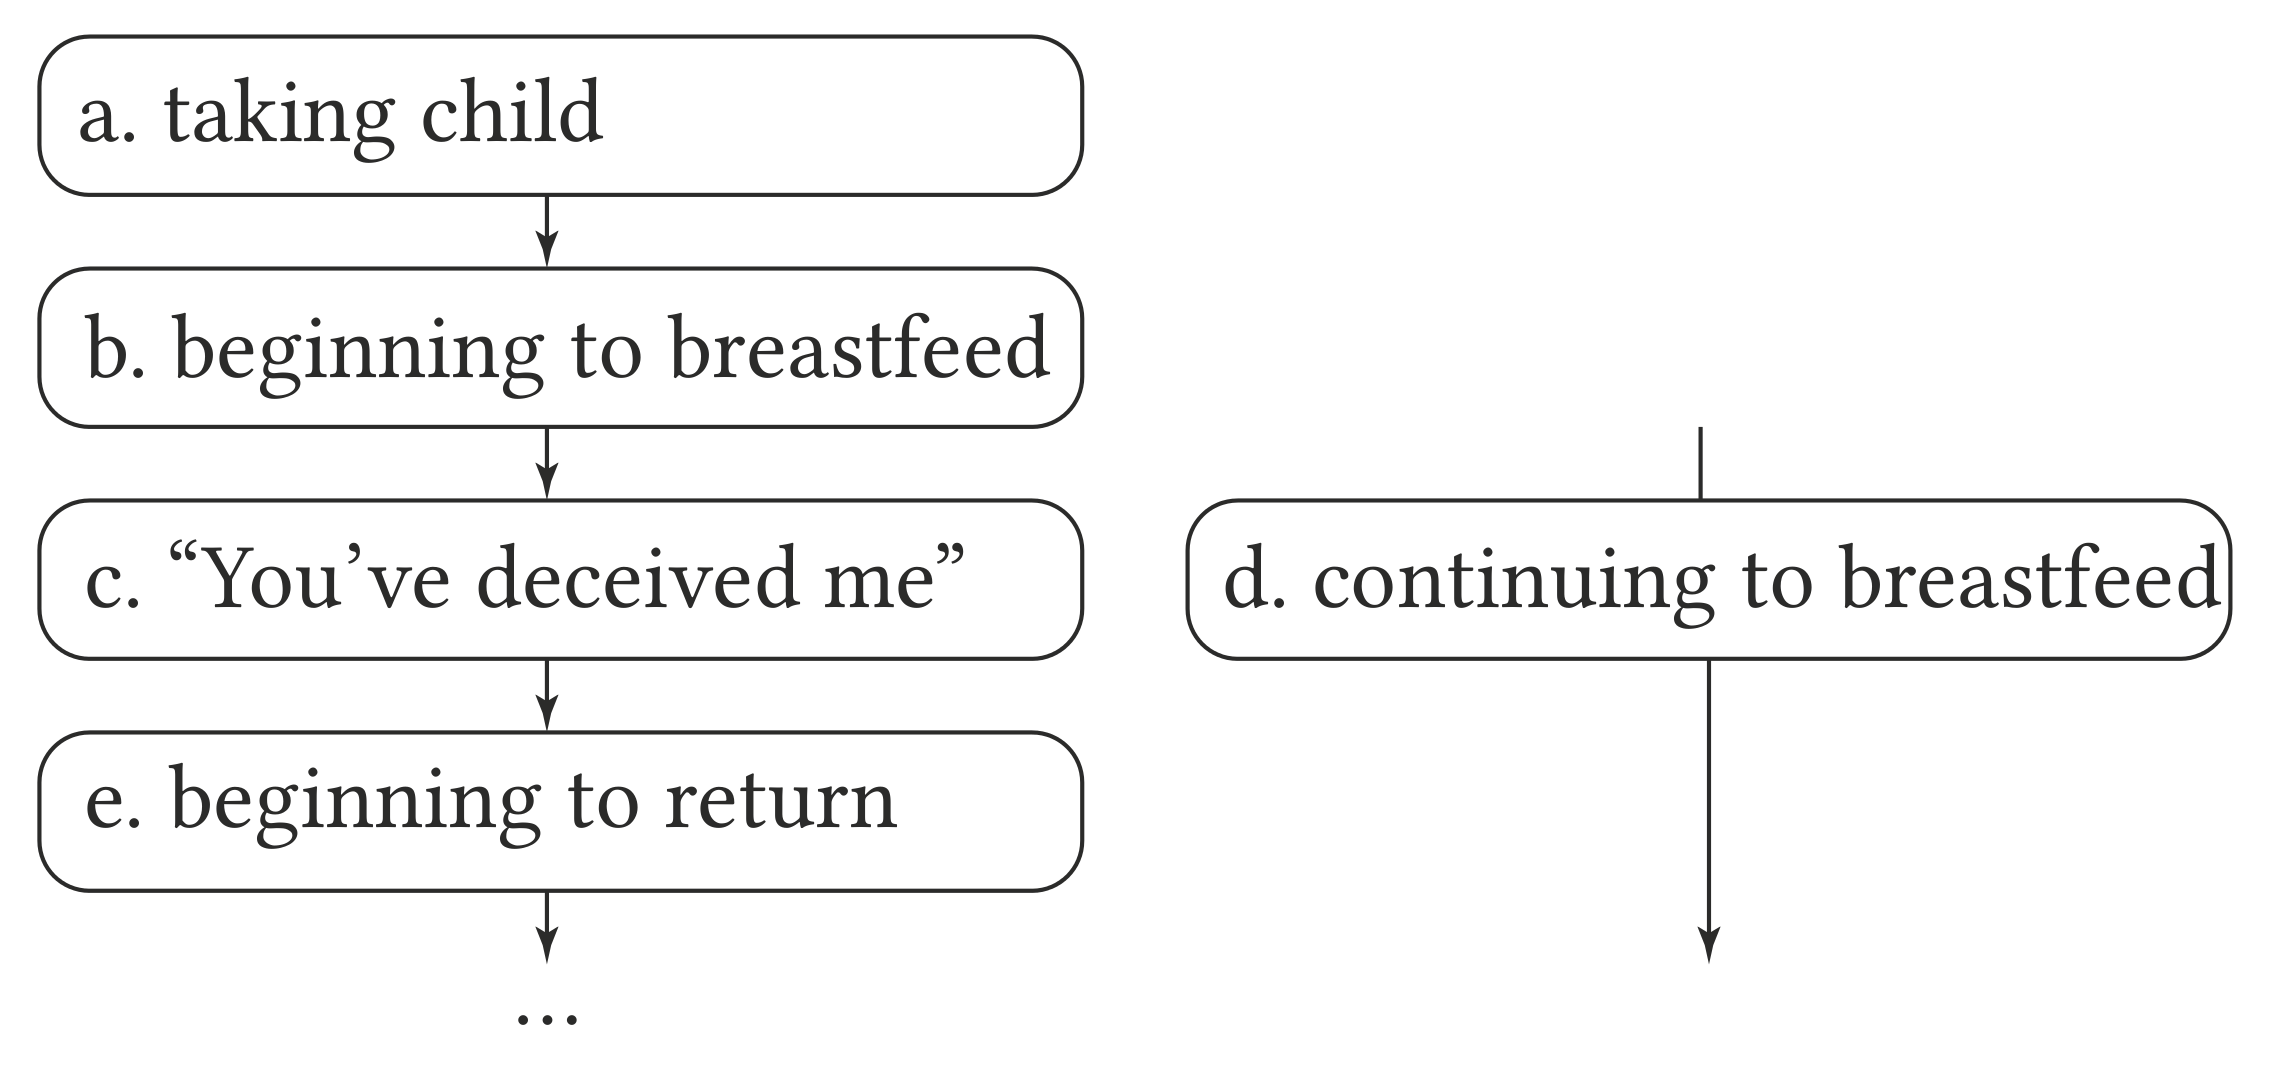
\includegraphics{figures/GrafikRelativeOrderThrowAway.png}
\caption{Relative event order of  (\ref{exNarrProg2})}
\label{FigureRelativeOrderProgressives1}
\end{center}
\end{figure}

\begin{exe}
\ex\label{exNarrProg2}
\begin{xlist}
\ex\label{exNarrProg2Sentence1}\gll a-lɪnkʊ-mmw-eg-a ʊ-mw-anaake\\
1-\textsc{narr}-1-take-\textsc{fv} \textsc{aug}-1-his\_child\\
\glt \lq She took her child.'
\ex\label{exNarrProg2Sentence2}\gll a-lɪnkw-end-a n=ʊ-kʊ-tɪ fi, ʊ-kw-and-a ʊ-kʊ-mm-ongesya\\
a-\textsc{narr}-walk/travel-\textsc{fv} \textsc{com}=\textsc{aug}-15-say what \textsc{aug}-15-begin-\textsc{fv} \textsc{aug}-15-1-breastfeed-\textsc{fv}\\
\glt \lq She then did what, began to breastfeed it.'
\ex\label{exNarrProg2Sentence3}\gll bo ʊ-kʊ-mm-ongesy-a a-lɪnkʊ-tɪ \lq\lq Haa! keet-a ʊʊ-syob-ile, gwe mw-inangʊ. ʊ-t-ile \lq\lq n-daag-ile ʊ-mw-ana''{}''\\
as 1-\textsc{prs}-1-breastfeed-\textsc{fv} 1-\textsc{narr}-say \textsc{interj} \phantom{\lq\lq}watch-\textsc{fv} \textsc{2sg.1sg}-deceive-\textsc{pfv} \textsc{2sg} 1-my\_companion \textsc{2sg}-say-\textsc{pfv} \textsc{1sg}-throw-\textsc{pfv} \textsc{aug}-1-child\\
\glt \lq As she was breastfeeding it, she [the other woman] said \lq\lq Haa! Look, you've deceived me, my friend. You said \lq\lq I've thrown away the child.''{}''{}'
\ex \label{exNarrProg2Sentence4}\gll po jʊ-la \textbf{a}-\textbf{lɪnkw}-\textbf{endelel}-\textbf{a} ʊ-kʊ-mm-ongesy-a ʊ-mw-ana\\
then 1-\textsc{dist} 1-\textsc{narr}-continue-\textsc{fv} \textsc{aug}-15-1-breastfeed-\textsc{fv} \textsc{aug}-1-child\\
\lq That one continued to breastfeed the child.'
\ex \label{exNarrProg2Sentence5}
\gll jʊ-la a-lɪnkw-and-a ʊ-kʊ-buj-a ʊ-kʊ-bʊʊk-a kʊ-kʊ-n-keet-a ʊ-mw-anaake\\
1-\textsc{dist} 1-\textsc{narr}-begin-\textsc{fv} \textsc{aug}-15-return-\textsc{fv} \textsc{aug}-15-go-\textsc{fv} 17-15-1-look-\textsc{fv} \textsc{aug}-1-child\\
\glt \lq That one began returning, going to look for her child.' [Throw away the child]
\end{xlist}
\end{exe}

\largerpage
Example (\ref{exNarrProg3}) depicts the beginning of a race between Hare and Tugutu, a type of bird. While Tugutu remains at the start (\ref{exNarrProg3Sentence4}), Hare does run (\ref{exNarrProg3Sentence2}, \ref{exNarrProg3Sentence5}). Hare's act of running is construed as an ongoing activity contemporaneous with his acts of speaking (\ref{exNarrProg3Sentence3}) and completing the first mile (\ref{exNarrProg3Sentence6}). \figref{FigureRelativeOrderProgressives2} illustrates this as a flow chart.

\begin{exe}
\ex Context: Hare and Tugutu are running a race.
\label{exNarrProg3}
\begin{xlist}
\ex \label{exNarrProg3Sentence1} \gll a-lɪnkʊ-tɪ \textup{\lq\lq}oko kalʊlʊ! tʊ-bop-ege leelo!\textup{''}\\
1-\textsc{narr}-say \phantom{\lq\lq}\textsc{interj} hare(1) \textsc{1pl}-run-\textsc{ipfv.subj} now/but\\
\glt \lq He [Tugutu] said \lq\lq Here we go, Hare! Let's run now!''

\ex\label{exNarrProg3Sentence2} \gll po kalʊlʊ \textbf{a}-\textbf{lɪnkʊ}-\textbf{bop}-\textbf{a}\\
then hare(1) 1-\textsc{narr}-run-\textsc{fv}\\
\glt \lq Hare ran/was running.'

\ex \label{exNarrProg3Sentence3}\gll a-lɪnkʊ-tɪ \textup{\lq\lq}lɪnga tʊ-bop-ile a-ma-elɪ jɪ-mo n-gʊ-kʊ-koolel-a ʊkutɪ \textup{\lq\lq}bʊle, mwa=n-dugutu, ʊ-li-po?\textup{''} gw-itɪk-e ʊ-tɪ \textup{\lq\lq}ee, n-di=po\textup{''{}''}\\
1-\textsc{narr}-say \phantom{\lq\lq}if/when \textsc{1pl}-run-\textsc{pfv} \textsc{aug}-6-mile(<EN) 9-one \textsc{1sg}-\textsc{prs}-\textsc{2sg}-call-\textsc{fv} \textsc{comp} \phantom{\lq\lq}\textsc{q} matronym=9-type\_of\_bird \textsc{2sg}-\textsc{cop}=16 \textsc{2sg}-agree-\textsc{subj} \textsc{2sg}-say.\textsc{subj} \phantom{\lq\lq}yes \textsc{1sg}-\textsc{cop}=16\\
\glt \lq He said \lq\lq When we've run one mile, I'll call you saying \lq\lq Mr. Tugutu are you there?'' You shall answer \lq\lq Yes, I'm here.''{}''{}'\footnote{The narrator oscillates between placing the loanword for \lq mile' in noun class 6, thus re-analyzing /ma/ as a prefix, and placing it in noun class 9a, the default for loans.}

\ex \label{exNarrProg3Sentence4} \gll po bo b-and-ile ʊ-kʊ-bop-a jʊ-la mwa=n-dugutu a-a-syeele pala$\sim$pa-la\\
then as 2-begin-\textsc{pfv} \textsc{aug}-15-run-\textsc{fv} 1-\textsc{dist} matronym=9-t.o.bird 1-\textsc{pst}-remain.\textsc{pfv} \textsc{redupl}$\sim$16-\textsc{dist}\\
\glt  ‎\lq When they had started to run that Mr. Tugutu had remained right there.'

\ex\label{exNarrProg3Sentence5}\gll po kalʊlʊ \textbf{a}-\textbf{lɪnkʊ}-\textbf{bop}-\textbf{a} mw-ene\\
then hare(1) 1-\textsc{narr}-run-\textsc{fv} 1-only\\
\glt \lq So Hare ran/was running alone.'

\ex \label{exNarrProg3Sentence6} \gll a-lɪnkʊ-mal-a a-ma-elɪ ga-mo\\
1-\textsc{narr}-finish-\textsc{fv} \textsc{aug}-6-mile 6-one\\
\glt \lq He completed one mile.' [Hare and Tugutu]
\end{xlist}
\end{exe}

\begin{figure}[hbt]
	\begin{center}
% 		\includegraphics{figures/GrafikRelativeOrderHareTugutu.eps}
		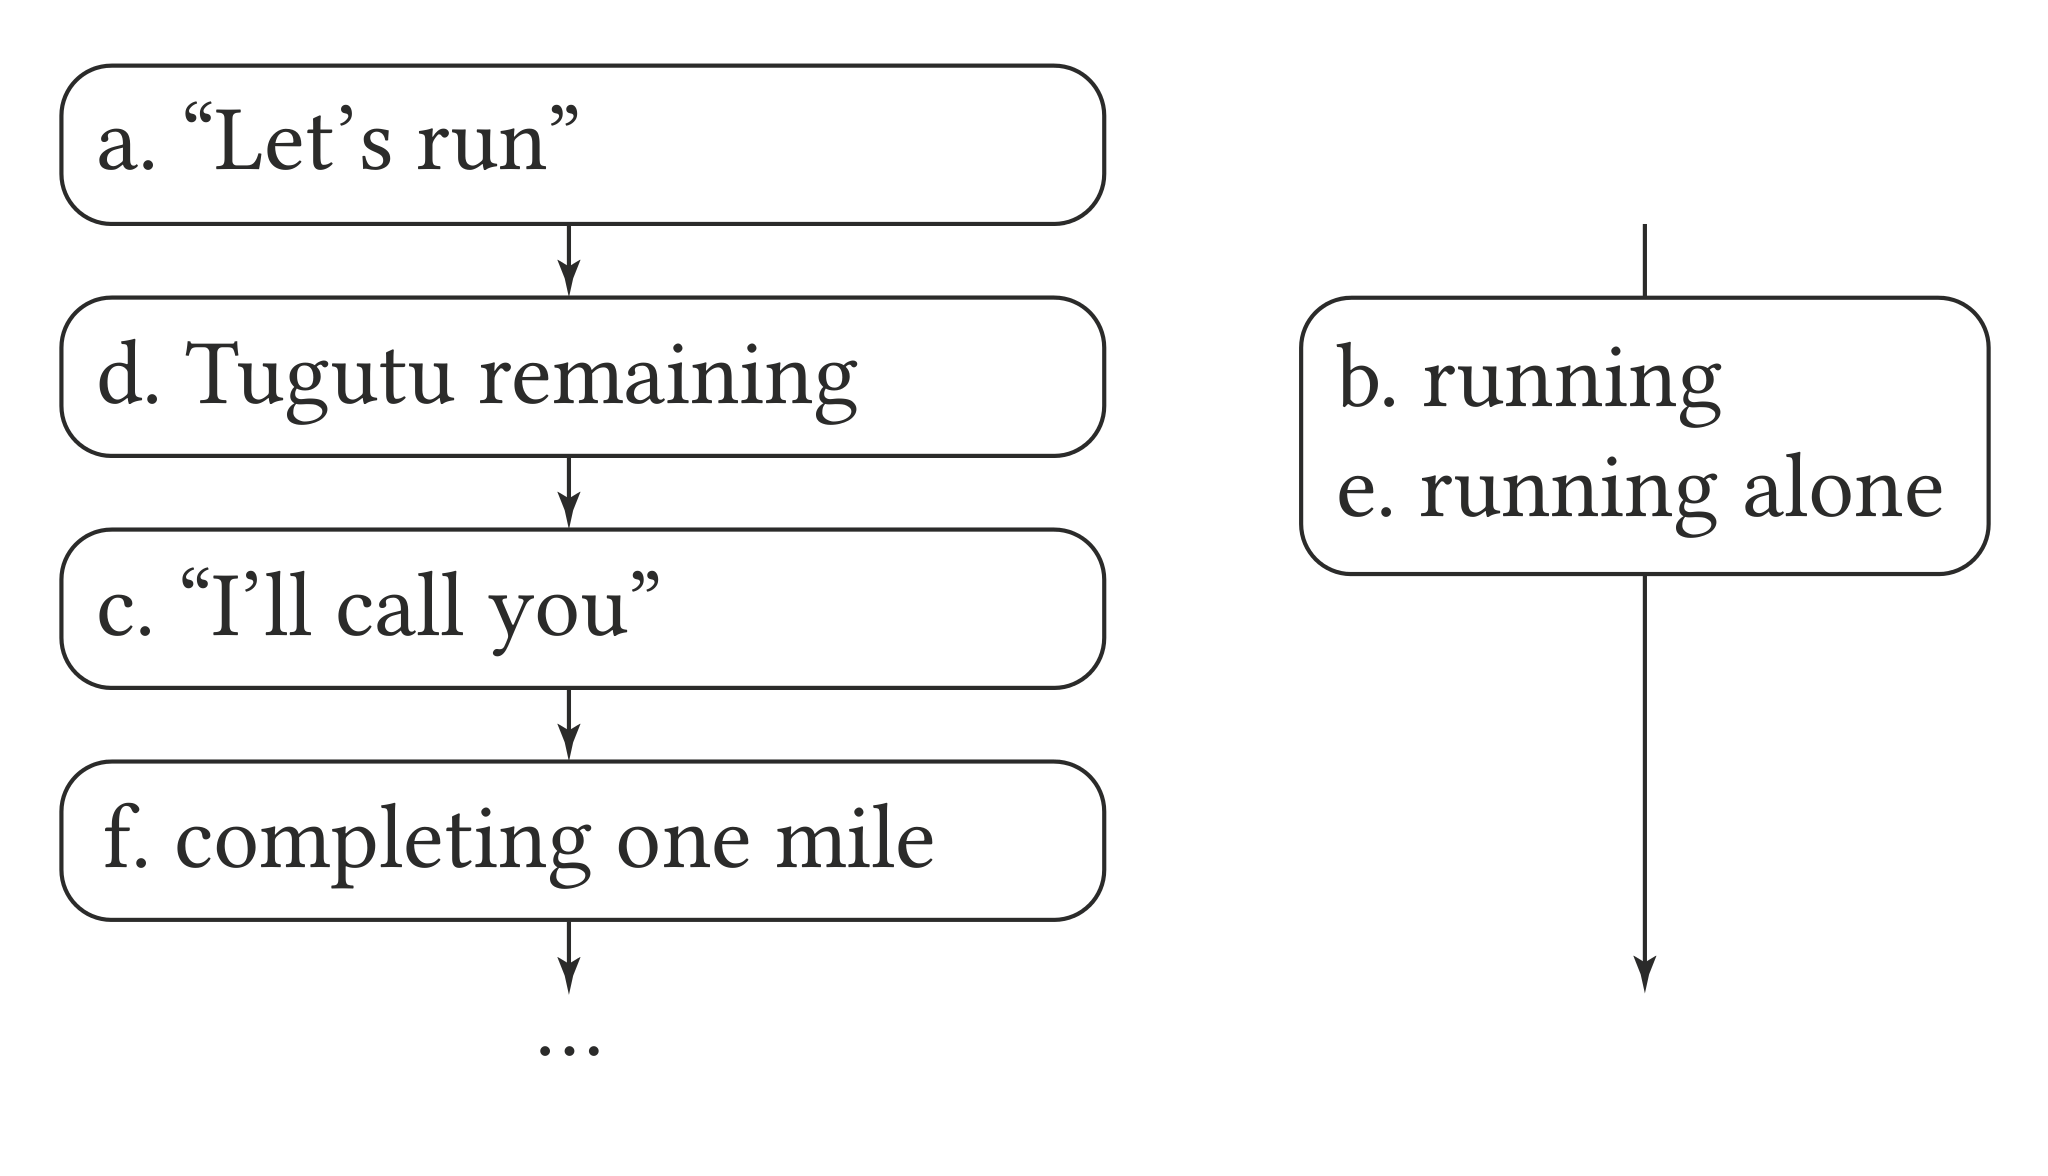
\includegraphics{figures/GrafikRelativeOrderHareTugutu.png}
		\caption{Relative event order of (\ref{exNarrProg3})}
		\label{FigureRelativeOrderProgressives2}
	\end{center}
\end{figure}

To summarize, the semantics of the Nyakyusa narrative tense include past time reference. Further, it is closely linked to episodic events and unspecified for grammatical aspect.

Considering that historically the narrative tense constituted a present tense\is{tense!present} construction, likely one carrying imperfective aspect,\is{aspect!imperfective} this indicates that its employment as a \isi{narrative present} has led to a profound re-adjustment of its semantics. For discussion see \citet{PersohnB2016}, where this shift in meaning is attributed to \citeauthor{FleischmanS1990}'s (\citeyear{FleischmanS1990}) \lq\lq plus interpretation'', by which a \isi{simple present} as the least specific TMA construction takes over the temporal (i.e. past tense)\is{tense!past} and aspectual\is{aspect!grammatical} meaning appropriate to context, as well as to a cross-Bantu tendency to have aspectually underspecified forms as narrative markers. \citet{RobarE2014} convincingly argues that the so-called \textit{wayyiqtol}-construction in \ili{Biblical Hebrew} underwent a comparable change, starting out as a \isi{simple present} whose extensive use as a \isi{narrative present} with the pragmatic function of signalling continuity has led to a bleaching of its original semantic content. In the case of Biblical Hebrew this has gone even further, allowing for the construction in question to take over any kind of tense,\is{tense} aspect\is{aspect!grammatical} or mood.\is{mood}
\is{aspect!grammatical|)}
\subsection{Sequentiality of events}
\label{NARRsequentiality}
Closely linked to the question of aspectual semantics\is{aspect!grammatical} is that of sequential ordering. At first the very concept of a narrative marker may suggest that the Nyakyusa narrative tense denotes sequential ordering of events. Moreover, on the basis of a \ili{Swahili} example taken as typical for Bantu, \citet[121]{NurseD2008} generalizes that ``the narrative explicitly sequences events [\ldots] and says that [\ldots] the second situation is later than the first''. \citet[111]{CoverR2010} cautions againt prematurely accepting such an assumption and observes that sequentiality is not part of the semantics of the narrative paradigms in \ili{Badiaranke} (Northern Atlantic). Similar observations have been made for the \textit{narrative}/\textit{consecutive tense} in the Senufo language \ili{Supyire} \citep{CarlsonR1994} and the so-called \textit{wayyiqtol}-construction in \ili{Biblical Hebrew} \citep{CookJ2004}. Concerning Bantu, \citet[277]{MorrisonME2011}, in her grammar of \ili{Bena} G63, notes that ``[the narrative tense] is \textit{often} best translated as \lq and then X' [emphasis added]'', while \citet{SeidelF2015} makes a similar observation for \ili{Yeyi} R41. Even for Nurse's model example, Swahili,\il{Swahili} a detailed examination shows that not all instances of the paradigm in question feature sequential ordering \citep[112f]{ContiniMoravaE1987}.

\citeauthor{LabovWWaletzkyJ1967}'s (\citeyear{LabovWWaletzkyJ1967}) framework of narrative analysis -- see \sectref{ToolsNarrativeAnalysis} -- provides us with a valuable tool to check whether the Nyakyusa narrative tense inherently encodes sequentiality. Assuming that it does encode an ordering of events would predict that no clause containing it can be displaced without changing the underlying order of events. That is, the narrative tense should only figure in those clauses that are classified as \textit{narrative clauses}.\is{clause types (Labov \& Waletzky)!narrative clause} The discussion of its aspectual semantics, however, has already shown that the narrative tense can have a progressive reading.\is{aspect!progressive} As a function of being ongoing, the eventualities in question overlap with other eventualities. That is, they can be displaced throughout a determined part of the text without changing the underlying order of events and can therefore be classified as \textit{restricted clauses}.\is{clause types (Labov \& Waletzky)!restricted clause} A few additional examples will illustrate the Nyakyusa narrative tense outside of narrative clauses.\is{clause types (Labov \& Waletzky)!narrative clause}

Another representative example of the narrative tense appearing in a restricted clause\is{clause types (Labov \& Waletzky)!restricted clause} is given in (\ref{exNARRnosequence1}). (\ref{exNARRnosequence1sentence1}) contains a husband's orders to his wife and (\ref{exNARRnosequence1sentence2}, \ref{exNARRnosequence1sentence3}) her carrying out these orders. Each step is dependent on the previous one. That is, these three clauses describe eventualities that happen in sequential order. The eventuality described in (\ref{exNARRnosequence1sentence4}), however, takes place simultaneously to the ones described in (\ref{exNARRnosequence1sentence2}, \ref{exNARRnosequence1sentence3}). This means that (\ref{exNARRnosequence1sentence4}) could be anticipated without changing the relative order of events, and is hence a restricted clause.\is{clause types (Labov \& Waletzky)!restricted clause} This becomes clear from the wider context of the story -- he goes on to clandestinely kill her father -- and is also signaled by spatial deixis: his actions take place at the deictic centre (\textit{kʊno} \lq here') while hers is viewed against the ground of an associated \isi{motion} event (see \sectref{jaAspectualizer} on the movement gram (\textit{j})\textit{a}). \figref{FigureRelativeOrderInLaw} is a visualization of the relative order of events.


\begin{exe}
\ex \label{exNARRnosequence1}
\begin{xlist}
\ex \label{exNARRnosequence1sentence1} \gll a-lɪnkʊ-n-koolel-a ʊ-n-kasi, a-lɪnkʊ-tɪ \textup{\lq\lq}n-kasi gw-angʊ, bʊʊk-e lɪlɪno ʊlʊ, k-ʊʊl-e ɪ-fi-lombe, ʊ-ka-sy-e ʊ-bʊ-fu, kʊ-ma-lʊʊka\textup{''}\\
1-\textsc{narr}-1-call-\textsc{fv} \textsc{aug}-1-wife 1-\textsc{narr}-say \phantom{\lq\lq}1-wife 1-\textsc{poss.1sg}, go-\textsc{subj} now/today now \textsc{itv}-buy-\textsc{subj} \textsc{aug}-8-maize \textsc{2sg}-\textsc{itv}-grind-\textsc{subj} \textsc{aug}-14-flour 17-6-store\\
\glt `He called his wife and said ``My wife, go right now, go buy maize, go grind flour, in the stores.''{}'

\ex \label{exNARRnosequence1sentence2} \gll nalooli ʊ-n-kiikʊlʊ \textbf{a}-\textbf{lɪnkw}-\textbf{a} \textbf{k}-\textbf{ʊʊl}-\textbf{a} ɪ-fi-lombe\\
really \textsc{aug}-1-woman 1-\textsc{narr}-go.\textsc{fv} 15-buy-\textsc{fv} \textsc{aug}-8-maize\\
\glt `She went and bought maize.'
\ex \label{exNARRnosequence1sentence3} \gll \textbf{a}-\textbf{lɪnkw}-\textbf{a} \textbf{kʊ}-\textbf{sy}-\textbf{a} ʊ-bʊ-fu kʊ-ma-lʊʊka\\
1-\textsc{narr}-go.\textsc{fv} 15-grind-\textsc{fv} \textsc{aug}-14-flour 17-6-shop\\
\glt `She went and ground flour at the stores.'
\ex \label{exNARRnosequence1sentence4} \gll kʊ-no ʊ-n̩-dʊme \textbf{a}-\textbf{lɪnkʊ}-\textbf{tendekesy}-\textbf{a} ʊ-tʊ-ndʊ, ɪ-fi-lwɪlo fy-a kʊ-n̩-gog-el-a ʊ-gwise\\
17-\textsc{prox} \textsc{aug}-1-husband 1-\textsc{narr}-prepare-\textsc{fv} \textsc{aug}-13-thing \textsc{aug}-8-poison 8-\textsc{assoc} 15-1-kill-\textsc{appl}-\textsc{fv} \textsc{aug}-his\_father(1)\\
\glt `Here her husband prepared things, poison to kill her father with.'
\ex \label{exNARRnosequence1sentence5} \gll a-a-gomok-a ʊ-mw-anike jʊ-la\\
1-\textsc{subsec}-return-\textsc{fv} \textsc{aug}-1-young\_person 1-\textsc{dist}\\
\glt `Then that young woman returned.' [Man and his in-law]
\end{xlist}
\end{exe}

\begin{figure}[hbt]
	\begin{center}
% 		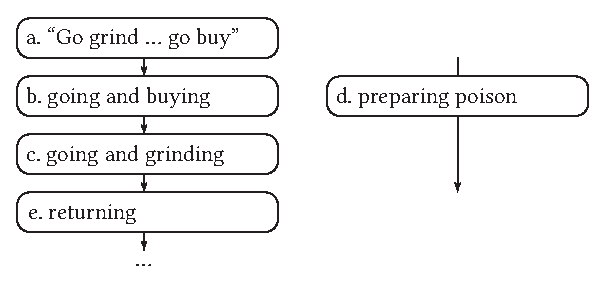
\includegraphics{figures/GrafikRelativeOrderInLaw.eps}
		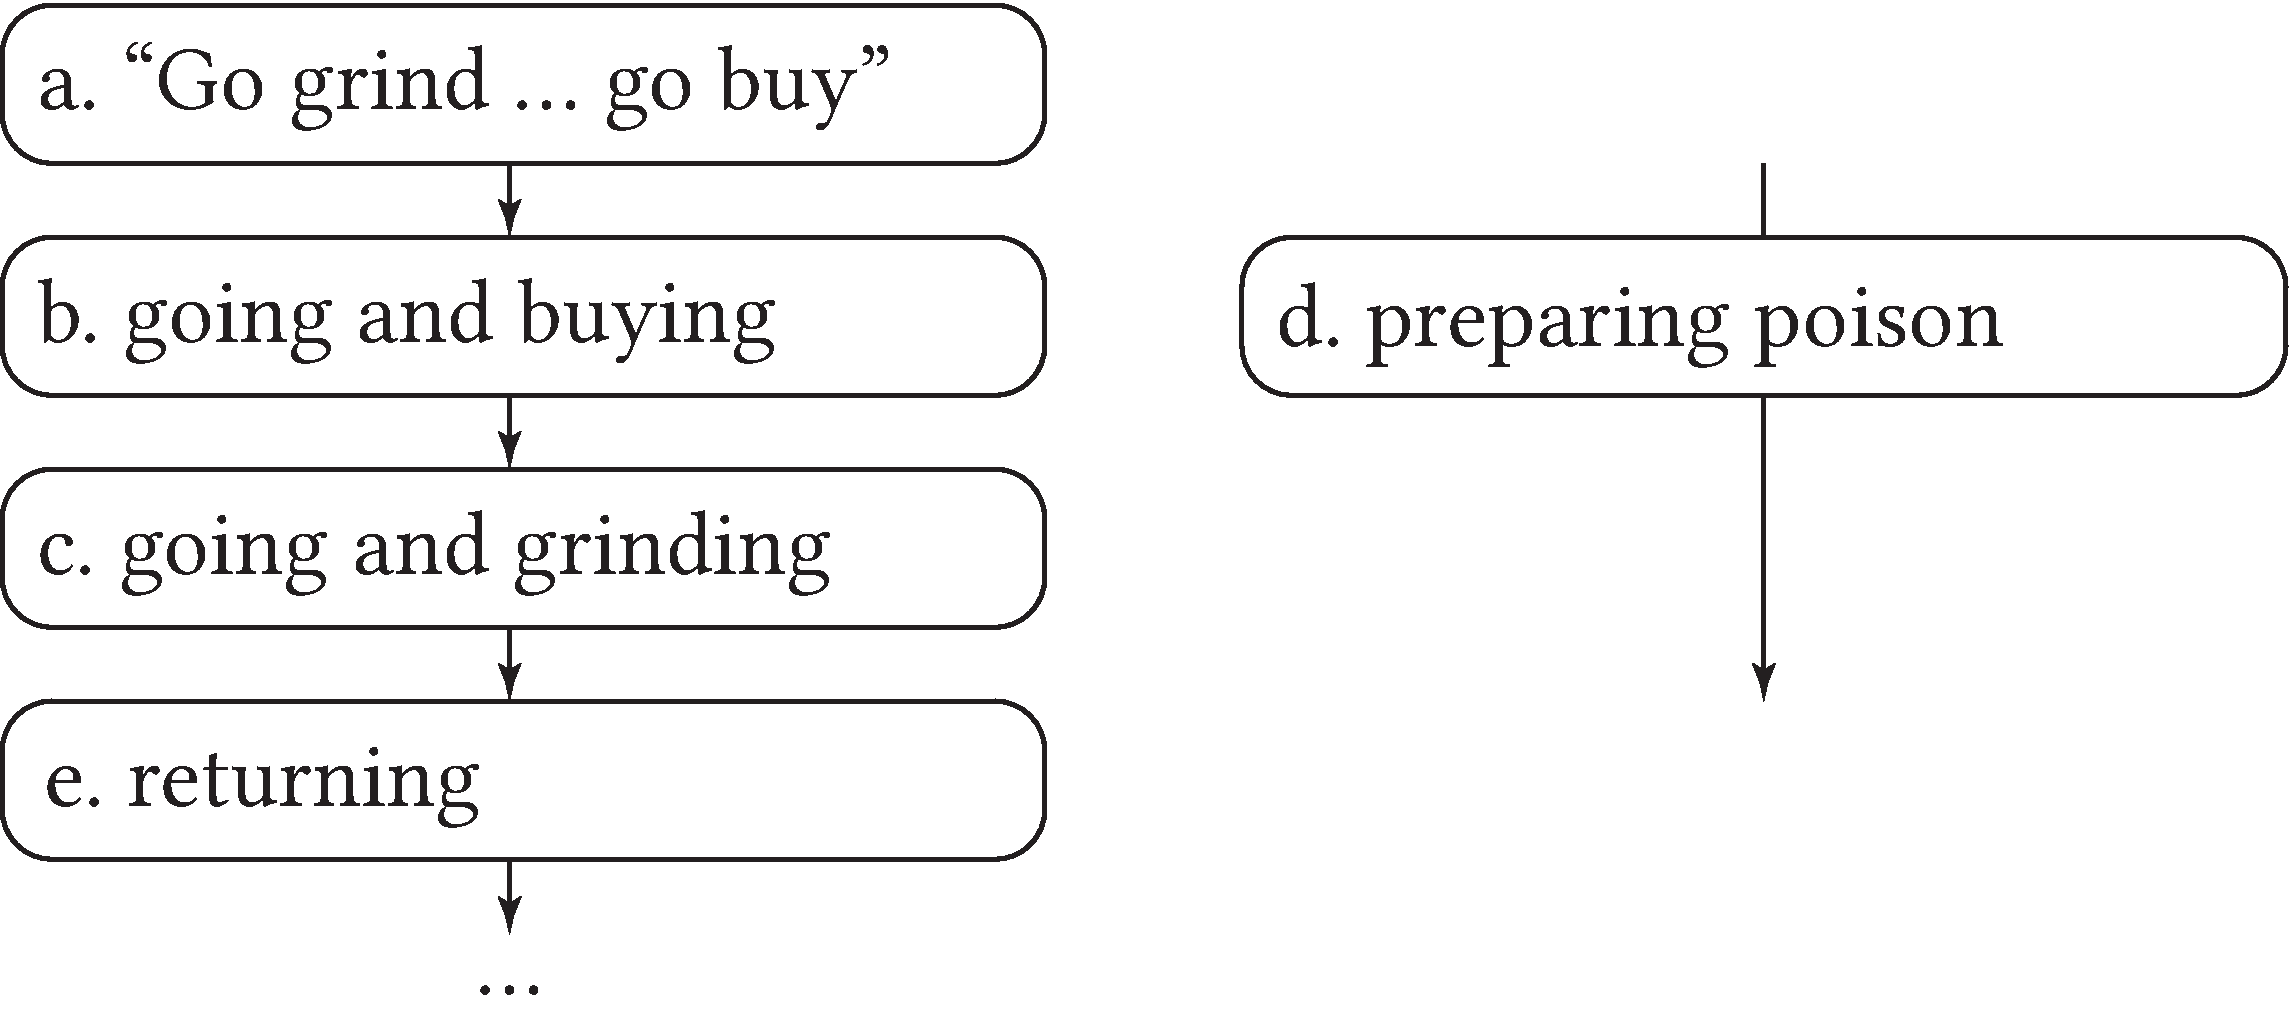
\includegraphics{figures/GrafikRelativeOrderInLaw.png}
	\end{center}
	\caption{Relative event order of (\ref{exNARRnosequence1})}
	\label{FigureRelativeOrderInLaw}
\end{figure}

The narrative tense also features in iconic repetitions that express a single extended eventuality (\ref{exNarrIconicRepetitions}). What is depicted in the three clauses in (\ref{exNarrIconicRepetitionsSentences1}) is not internally ordered. These clauses are thus classified as \textit{co-ordinate clauses}.\is{clause types (Labov \& Waletzky)!co-ordinate clause} The case of (\ref{exNarrIconicRepetitionsSentence2}) presents more difficulties: it is not entirely clear if the speech act depicted takes place during the protagonists' walking or if it is preceded by a stop.

\begin{exe}
\ex \label{exNarrIconicRepetitions}
\begin{xlist}
\ex \label{exNarrIconicRepetitionsSentences1} \gll po \textbf{ba}-\textbf{lɪnkw}-\textbf{end}-\textbf{a}, \textbf{ba}-\textbf{lɪnkw}-\textbf{end}-\textbf{a}, \textbf{ba}-\textbf{lɪnkw}-\textbf{end}-\textbf{a}\\
then 2-\textsc{narr}-walk/travel-\textsc{fv} 2-\textsc{narr}-walk/travel-\textsc{fv} 2-\textsc{narr}-walk/travel-\textsc{fv}\\
\glt \lq They walked, they walked, they walked.'
\ex \label{exNarrIconicRepetitionsSentence2} \gll ba-lɪnkʊ-tɪ \textup{\lq\lq}eh tʊ-kateele\textup{''}\\
2-\textsc{narr}-say \phantom{\lq\lq}\textsc{interj} \textsc{2pl}-be(come)\_tired.\textsc{pfv}\\
\glt \lq They said \lq\lq Eh, we're tired.''{}' [Throw away the child]
\end{xlist}
\end{exe}

Another case of the narrative tense featuring in co-ordinate clauses\is{clause types (Labov \& Waletzky)!co-ordinate clause} is given in
(\ref{exNARRnosequence2}). Clauses (\ref{exNARRnosequence2sentence1}, \ref{exNARRnosequence2sentence2}) describe eventualities that happen in sequence: the pepper only comes out of the bottles after the monkeys catch them. Clauses (\ref{exNARRnosequence2sentence3}--\ref{exNARRnosequence2sentence5}) however, describe various facets of one and the same eventuality. They can be freely swapped with each other, but are ordered relative to (\ref{exNARRnosequence2sentence2}).

\begin{exe}
\ex \label{exNARRnosequence2}
Context: People try to get rid of a group of thieving monkeys that devastate their fields. To fight them, they throw small bottles filled with pepper.
\begin{xlist}
\ex \label{exNARRnosequence2sentence1} \gll si-lɪnkw-angɪl-a m-mwanya\\
10-\textsc{narr}-catch-\textsc{fv} 18-high\\
\glt `They caught (the bottles) in mid air.'

\ex \label{exNARRnosequence2sentence2} \gll ɪ-m-bilipili jɪ-lɪnkʊ-sunyunduk-a n-tʊ-supa mu-la n=ʊ-kʊ-nyeel-el-a m-maa-so na m-mi-lomo \\
\textsc{aug}-9-pepper(<SWA) 9-\textsc{narr}-come\_out\_of-\textsc{fv} 18-13-bottle 18-\textsc{dist} \textsc{com}=\textsc{aug}-15-jump-\textsc{appl}-\textsc{fv} 18-6-eye \textsc{com} 18-4-lip\\
\glt `The pepper came out of the little bottles and flew into their eyes and mouths.'

\ex \label{exNARRnosequence2sentence3} \gll popaa$\sim$po ɪ-n-gambɪlɪ \textbf{si}-\textbf{lɪnkʊ}-\textbf{gw}-\textbf{a} paa-si paapo j-aa-lɪ n-galɪ fiijo\\
\textsc{redupl}$\sim$then \textsc{aug}-10-monkey 10-\textsc{narr}-fall-\textsc{fv} 16-below because 9-\textsc{pst}-\textsc{cop} 9-fierce \textsc{intens}\\
\glt `And so the monkeys fell down because it was very hot.'

\ex \label{exNARRnosequence2sentence4} \gll \textbf{si}-\textbf{lɪnkʊ}-\textbf{kuut}-\textbf{a} si-lɪnkʊ-tɪ, ``Ho! Ho! Ho!''\\
10-\textsc{narr}-cry-\textsc{fv} 10-\textsc{narr}-say \phantom{\lq\lq}\textsc{interj} \textsc{interj} \textsc{interj}\\
\glt `‎‎They cried and said, ``Ho! Ho! Ho!''{}'
\ex \label{exNARRnosequence2sentence5} \gll si-mo \textbf{si}-\textbf{lɪnkʊ}-\textbf{gw}-\textbf{a} paa-si, \textup{\lq\lq}puu!\textup{''}\\
10-one 10-\textsc{narr}-fall-\textsc{fv} 16-below \phantom{\lq\lq}of\_falling\_down\\
\glt `Some fell down, ``Splat!''{}' [Thieving monkeys]
\end{xlist}
\end{exe} %d.h. einen restricted clause

To conclude, the Nyakyusa narrative tense appears in narrative clauses\is{clause types (Labov \& Waletzky)!narrative clause} as well as in restricted\is{clause types (Labov \& Waletzky)!restricted clause} and co-ordinate clauses.\is{clause types (Labov \& Waletzky)!co-ordinate clause} This shows that sequential order is not one of its semantic features. The fact that most eventualities depicted in this paradigm stand in sequence is a mere correlate of the predominantly iconic ordering of narrative discourse.

However, it is important to note that while in examples (\ref{exNarrProg2}--\ref{exNARRnosequence2}) not all the eventualities depicted in the narrative tense are ordered relative to each other, no out-of-sequence uses are attested. The narrative tense does not feature in free clauses.\is{clause types (Labov \& Waletzky)!free clause}  Although it does feature in certain restricted clauses,\is{clause types (Labov \& Waletzky)!restricted clause} this is limited to clearly defined episodic situations; see also \sectref{NARRpast}. That is, the narrative tense does not feature in clauses that serve as orientation; see also \sectref{NarrativeMarkersUseDistribution}. Lastly, flashbacks in narrative discourse are exclusively expressed by means of the past perfective (\sectref{PastPFVNarrativeDiscourseSupportive}).
\subsection{Summary}
To summarize, the Nyakyusa narrative tense goes back to a \isi{simple present} or present progressive\is{aspect!progressive} used as a narrative present.\is{narrative present} In the present-day language, it is the most common dedicated narrative marker (see \sectref{NarrativeMarkersQuantitativeDistribution}), whose semantics include reference to the past time. It is unspecified for grammatical aspect,\is{aspect!grammatical} but restricted to episodic situations and thus the narrative storyline. The narrative tense by itself does not encode sequential ordering. Instead it is attested with sequential as well as simultaneous eventualities. The employment of the narrative tense, like the subsecutive,\is{subsecutive} is dependent on an otherwise established situation and forms part of a larger pattern, in which narrative discourse is constructed around the notion of \isi{thematic continuity} and discontinuity.  Given that the narrative tense is a dedicated marker of narrative  discourse, the narrative tense can further be understood as a metalinguistic\is{component of meaning!metalinguistic} signal of narrativity.
\is{narrative tense|)}
\section{Subsecutive}\label{Subsecutive}\is{subsecutive|(}
This section deals with the subsecutive, Nyakyusa's second dedicated narrative marker. In the following sub-sections, first its formal makeup and possible diachronic source will be discussed (\sectref{SubsecutiveIntroduction}), then some restrictions on the use of the subsecutive will be broached (\sectref{SubsecutiveAndNarrative}). This is followed by an overview of its semantics together with its basic textual function\is{component of meaning!textual} (\sectref{SubsecutiveSemantics}), as these two facets are inseparably linked. The latter are then illustrated by a number of common uses (\sectref{SubsecutiveCommon}) before going on to discuss a number of examples of the subsecutive without strict temporal progression (\sectref{SubsecutiveCounterExamples}).
\subsection{Formal makeup}\label{SubsecutiveIntroduction}
\largerpage
The subsecutive is formed by a prefix \textit{a}- in the post-initial slot, together with the default final vowel -\textit{a}.

\begin{exe}
\ex \textit{twajoba} `then we spoke'
\end{exe}

There is no \isi{negative} counterpart to the subsecutive. In elicitation, negation of the subsecutive through the \isi{negative} \isi{auxiliary} \textit{sita} plus an augmentless infinitive,\is{infinitive} parallel to what is found for the \isi{narrative tense} (see \sectref{sectionNarrativeTenseFormalAspects}), was accepted. This pattern is, however, not attested in the text corpus. Like the narrative tense,\is{narrative tense} the subsecutive is attested only in independent clauses.

\citet{SchumannK1899} and \citet{EndemannC1914} consider the subsecutive a simple past,\is{tense!past}\footnote{They refer to it as \textit{Imperfektum}. In the German tradition this term is sometimes used as a synonym for \textit{Präteritum} (preterite/simple past\is{tense!past}), which fits their description.} an analysis that is, however, not corroborated by its usage in text collections from the chronolect described by them (\citealt{BergerP1933}; \citealt{BusseJ1942}; \citeyear{BusseJ1949}). The term \textit{subsecutive} has been adopted from \citeauthor{MwangokaNVoorhoeveJ1960b}'s (\citeyear{MwangokaNVoorhoeveJ1960b}) grammatical sketch. Some of the uses of this construction found in \citeauthor{MeyerT1989}'s (\citeyear{MeyerT1989}) ethnological notes, originally gathered at the turn of the twentieth century, indicate that the subsecutive constitutes a former present perfective\is{tense!present}\is{aspect!perfective} or anterior.\is{aspect!anterior} Such an origin is also indicated by the \isi{evidential} of report \textit{baatɪ} (\sectref{defectiveti}), most likely from \lq they (have) said', and the two variants of the courtesy formula \textit{naapela} / \textit{mbelile} `please', the former featuring the subsecutive, the latter the present perfective.\is{tense!present}\is{aspect!perfective} What is more, as the following discussion will show, a diachronic source along the lines of a present perfective\is{tense!present}\is{aspect!perfective} or anterior\is{aspect!anterior} is consistent with the meaning and use of the subsecutive in the present day language.

\subsection{Restrictions on use}\label{SubsecutiveAndNarrative}
As discussed in \sectref{NarrativeMarkersQuantitativeDistribution}, the subsecutive is the less frequent of Nyakyusa's two narrative markers, considering the absolute frequency within a given text as well as across the entire corpus of oral narratives. Unlike the narrative tense,\is{narrative tense} which no narrative in the corpus can do without, the subsecutive is completely absent from nearly half of all oral narratives. What is more, the subsecutive is subject to normative restrictions.

To begin with, the subsecutive does not appear in written narratives, with the exception of one sole token. In discussions of examples from oral narratives, some of the language assistants stated that the subsecutive is a common device in storytelling, but followed up by saying that it would be inappropriate in the written medium.\footnote{A similar phenomenon has been observed in \ili{Malila} M24, where speakers would use the present perfective,\is{tense!present}\is{aspect!perfective} likewise of the shape \textit{a}-\textsc{vb}-\textit{a}, in the storyline of oral narratives, but insisted that it would be inappropriate for a written story \citep[24]{EatonH2015a}.} Other language assistants rejected any constructed examples containing the subsecutive but then used it themselves in oral texts. A few speakers even considered this construction a \ili{Ndali} intrusion into their language. This assessment can easily be rejected, given the construction's apparent age, the fact that it is found in the eastern varieties of Nyakyusa (\sectref{InternalClassiffication}), whereas \ili{Ndali} is one of Nyakyusa's western neighbours, and its distribution, which does not resemble that of its \ili{Ndali} cognate as described by \citet{BotneR2008}.

\largerpage
\subsection{Semantics and basic textual function}\label{SubsecutiveSemantics}
As discussed in \sectref{NARRpast}, narrative markers across languages differ, among other ways, in their possible temporal reference. The Nyakyusa subsecutive, like the narrative tense,\is{narrative tense} is attested only with temporal reference preceding the time of speech. This is corroborated by negative evidence from elicitation, where it was rejected for future\is{tense!future} predictions (\ref{exSubsecNotFuture1}, \ref{exSubsecNotFuture2}) as well as in a timeless \isi{generic} use (\ref{exSubsecNotGeneric}).
\begin{exe}


\newpage 
\ex \label{exSubsecNotFuture1} Context: A young man's plans for the future.
\begin{xlist}
\ex[]{\gll bo n-gʊl-ile a=n-gʊ-jeng-a ɪɪ-nyumba ɪɪ-nywamu\\
as \textsc{1sg}-grow-\textsc{pfv} \textsc{fut}=\textsc{1sg}-\textsc{prs}-build-\textsc{fv} \textsc{aug}-house(9) \textsc{aug}-big(9)\\}
\ex[\#]{\gll \textbf{n}-\textbf{aa}-\textbf{tim}-\textbf{a} ɪɪ-ng'ombe pa-ka-aja\\
\textsc{1sg}-\textsc{subsec}-herd-\textsc{fv} \textsc{aug}-cow(10) 16-12-homestead\\
\glt (intended: \lq When I am grown up, I will build a big house. Then I will herd cows at home.')}
\end{xlist}
\ex \label{exSubsecNotFuture2} Context: Talking about the speaker's plans for tomorrow.
\begin{xlist}
\ex[]{\gll kɪ-laabo a=n-gʊ-kin-a ʊ-m-pɪla\\
7-tomorrow \textsc{fut}-\textsc{1sg}-\textsc{prs}-play-\textsc{fv} \textsc{aug}-3-ball\\}
\ex[\#]{\gll bo m-mal-ile pa-kʊ-kin-a \textbf{n}-\textbf{aa}-\textbf{bʊʊk}-\textbf{a} kʊ-n-nuguna gw-angʊ kʊ-kʊ-ly-a nagwe ɪ-fi-ndʊ fy-a pa-muu-si\\
as \textsc{1sg}-finish-\textsc{pfv} 16-15-play-\textsc{fv} \textsc{1sg}-\textsc{subsec}-go-\textsc{fv} 17-1-younger\_sibling\_of\_same\_sex 1-\textsc{poss.1sg} 17-15-eat-\textsc{fv} \textsc{com.1} \textsc{aug}-8-food 8-\textsc{assoc} 17-3-daytime\\
\glt (intended: \lq Tomorrow I will play football. When I am done playing, I will go to my younger brother to have lunch with him.')}
\end{xlist}
\ex \label{exSubsecNotGeneric} Context: Describing the process of preparing stiff porridge.
\begin{xlist}
\ex[]{\gll bi-kʊ-kosy-a ʊ-m-ooto\\
2-\textsc{prs}-light-\textsc{fv} \textsc{aug}-3-fire\\}
\ex[\#]{\gll \textbf{b}-\textbf{aa}-\textbf{suk}-\textbf{a} ɪ-fy-a kʊ-pɪɪj-ɪl-a\\
2-\textsc{subsec}-wash-\textsc{fv} \textsc{aug}-8-\textsc{assoc} 15-cook-\textsc{appl}-\textsc{fv}\\}
\ex[\#]{\gll \textbf{b}-\textbf{aa}-\textbf{bɪɪk}-\textbf{a} a-m-ɪɪsi pa-m-ooto \ldots\\
2-\textsc{subsec}-put-\textsc{fv} \textsc{aug}-6-water 16-3-fire\\
\glt (intended: \lq They light the fire. Then they wash the cooking utensils. Then they put the water on the fire \ldots')}
\end{xlist}
\end{exe}

Like the narrative tense,\is{narrative tense} the subsecutive is only attested in episodic sentences, that is reports of specific events or occasions; see \sectref{NARRpast} for discussion. Negative evidence from elicitation shows that even within the past\is{tense!past} it cannot continue habituals\is{aspect!habitual} or generics:\is{aspect!generic}

\begin{exe}
\ex
\begin{xlist}
\ex[]{\gll ijolo ba-a-mog-aga fiijo\\
old\_times 2-\textsc{pst}-dance-\textsc{ipfv} \textsc{intens}\\
}
\ex[]{\gll ba-a-fwal-aga kanunu fiijo\\
2-\textsc{pst}-dress/wear-\textsc{ipfv} well \textsc{intens}\\}
\ex[\#]{\gll b-oog-a\\
2-\textsc{subsec}.bathe-\textsc{fv}\\}
\ex[\#]{\gll ba-a-sanjʊl-a n=ɪɪ-nywili \ldots\\
2-\textsc{subsec}-comb-\textsc{fv} \textsc{com}=\textsc{aug}-hair(10) {}\\
\glt (intended: \lq Long ago they used to dance a lot. They dressed well. They bathed. They combed their hair \ldots')}
\end{xlist}
\end{exe}

Concerning its aspectual semantics,\is{aspect!grammatical} the subsecutive, unlike the narrative tense,\is{narrative tense} always has a perfective reading;\is{aspect!perfective} see \sectref{PerfectivityCompletion} for a discussion of perfectivity. What is more, the subsecutive explicitly marks a step forward in the text. In this it can be understood as a verbal variety of what \citet{DooleyRALevinsohnSH2000} call a \lq\lq developmental marker'', which \lq\lq indicate[s] that the material so marked represents a new development in the story or argument, as far as the author's purpose is concerned'' (p. 48). This function will become clear when looking at its common uses in \sectref{SubsecutiveCommon}. In the majority of cases, the narrative development goes along with an advancement of narrative time. Thus, the subsecutive nearly exclusively occurs in narrative clauses,\is{clause types (Labov \& Waletzky)!narrative clause} i.e. those clauses that stand in fixed sequence; see \sectref{ToolsNarrativeAnalysis} for \citeauthor{LabovWWaletzkyJ1967}'s (\citeyear{LabovWWaletzkyJ1967}) classification of independent clauses within narratives. Unlike the narrative tense,\is{narrative tense} the subsecutive is not attested in restricted clauses.\is{clause types (Labov \& Waletzky)!restricted clause} A few cases of the subsecutive in co-ordinate\is{clause types (Labov \& Waletzky)!co-ordinate clause} clauses will be examined more closely in \sectref{SubsecutiveCounterExamples}. Closely linked to this distribution, the only type of temporal adverbials the subsecutive is attested with is adverbials referring to a subsequent time span. (\ref{exSubsecutiveSerieSentence2}) illustrates the latter for a temporal clause,\is{subordinate clauses!temporal clause} (\ref{exSubsecutiveSerieSentence5}) for the adverbial \textit{kɪlaabo} \lq tomorrow, next day'. 

\begin{exe}
\ex Context: A girl has eloped with a man. Her father has found out where they are.
\begin{xlist}
\ex \label{exSubsecutiveSerieSentence1} \gll po piitaasi ʊ-n-nyambala jʊ-la a-lɪnkʊ-j-a mu-ndʊ gw-a kʊ-fung-a ɪɪ-safalɪ j-aake j-aa kʊ-bʊʊk-a kʊ-no ba-li=ko ba-la, kʊ-kʊ-mel-a ɪ-fy-ʊma\\
then later \textsc{aug}-1-man 1-\textsc{dist} 1-\textsc{narr}-be(come)-\textsc{fv} 1-person 1-\textsc{assoc} 15-tie-\textsc{fv} \textsc{aug}-journey(9)(<SWA) 9-\textsc{poss.sg} 9-\textsc{assoc} 15-go-\textsc{fv} 17-\textsc{prox} 2-\textsc{cop}=17 2-\textsc{dist} 17-15-claim-\textsc{fv} \textsc{aug}-8-rich\\
\glt \lq Then later that man started to set out for where they were, in order to claim the brideprice.'
\ex \label{exSubsecutiveSerieSentence2}\gll \textbf{bo} \textbf{a}-\textbf{fik}-\textbf{ile} kʊ-la \textbf{b}-\textbf{a}-\textbf{mmw}-\textbf{ambɪlɪl}-\textbf{a} kanunu\\
as 1-arrive-\textsc{pfv} 17-\textsc{dist} 2-\textsc{subsec}-1-receive-\textsc{fv} well\\
\glt \lq When he arrived there, they received him well.'

\ex \gll a-a-ly-a\\
1-\textsc{subsec}-eat-\textsc{fv}\\
\glt \lq He ate.'

\ex \gll a-a-gon-a\\
1-\textsc{subsec}-rest-\textsc{fv}\\
\glt \lq He slept.'

\ex \label{exSubsecutiveSerieSentence5} \gll po \textbf{kɪ}-\textbf{laabo} \textbf{a}-\textbf{mmw}-\textbf{eg}-\textbf{a} ʊ-n-kyameni n=ʊ-kʊ-m̩-bʊʊl-a ɪ-si si-n-twele pa-la\\
then 7-tomorrow 1.\textsc{subsec}-1-take-\textsc{fv} \textsc{aug}-1-chairman(<EN) \textsc{com}=\textsc{aug}-15-1-tell-\textsc{fv} \textsc{aug}-\textsc{prox.10} 10-1-carry.\textsc{pfv} 16-\textsc{dist}\\
\glt \lq The next day he contacted  a chairman and told him what brought him there.' [Man and his in-law]

\end{xlist}
\end{exe}

Consecutive clauses featuring the subsecutive are generally understood as depicting an ordered sequence of completed\is{completion} eventualities building on each other, as in (\sectref{exSubsecutiveSerieSentence1}--\ref{exSubsecutiveSerieSentence5}). A few exceptions, in which a sequence of clauses featuring the subsecutive group together, will be examined in \sectref{SubsecutiveCounterExamples}.

Note at this point that the opposition between the \isi{narrative tense} and the subsecutive in the present-day language cannot be reduced merely to one of grammatical aspect. As discussed in \sectref{NARRpast}, the \isi{narrative tense} is best understood as unspecified for aspect and allows for a perfective-like\is{aspect!perfective} reading, too. Rather, these two paradigms form an opposition between the default, all-purpose narrative tense on the one hand and the subsecutive as the more restricted, specifically perfective\is{aspect!perfective} marker of a narrative development on the other.

\subsection{Common occurrences}
\label{SubsecutiveCommon}
Many tokens of the subsecutive in the corpus are found in discernible, reoccurring environments. To begin with, it is found in pairings with the narrative tense,\is{narrative tense} as in (\ref{exSubsecutivePreparationResultSentence2}, \ref{exSubsecutivePreparationResultSentence3}) and (\ref{exSubsecutivePreparationResultSentence5}, \ref{exSubsecutivePreparationResultSentence6}), in which a situation is depicted first in its inception or preparation and then in its culmination.


\begin{exe}
\ex \label{exSubsecutivePreparationResult}
\begin{xlist}
\ex \gll po ba-lɪnkw-and-a b-oope bo bʊ-k-iile n=ʊ-lʊ-bʊnjʊ\\
then 2-\textsc{narr}-begin-\textsc{fv} 2-also as 14-dawn-\textsc{pfv} \textsc{com}=\textsc{aug}-11-morning\\
\glt \lq Early in the morning they started.'

\ex \label{exSubsecutivePreparationResultSentence2}\gll ba-lɪnkʊ-j-a b-andʊ ba-a k-oog-a b-ooga\\
2-\textsc{narr}-be(come)-\textsc{fv} 2-person 2-\textsc{assoc} 15-bathe-\textsc{fv} 14-bath\\
\glt \lq They began to bath.'

\ex \label{exSubsecutivePreparationResultSentence3}\gll \textbf{ba}-\textbf{a}-\textbf{fwal}-\textbf{a} kanunu\\
2-\textsc{subsec}-dress/wear-\textsc{fv} well\\
\glt \lq They got dressed up.'

\ex \label{exSubsecutivePreparationResultSentence4}\gll ba-lɪnkʊ-j-a b-andʊ ba-a kʊ-piny-a ɪ-mi-sigo gy-abo n=ʊ=kʊ-bʊʊk-a\\
2-\textsc{narr}-be(come)-\textsc{fv} 2-person 2-\textsc{assoc} 15-bind-\textsc{fv} \textsc{aug}-4-burden 4-\textsc{poss.pl} \textsc{com}=\textsc{aug}-15-go-\textsc{fv}\\
\glt \lq They began to bind their things and go.'

\ex \label{exSubsecutivePreparationResultSentence5} \gll a-lɪnkʊ-pimb-a ʊ-bʊ-fu bw-ake n̩goosi\\
1-\textsc{narr}-load-\textsc{fv} \textsc{aug}-14-flour 14-\textsc{poss.sg} N.\\
\glt \lq Ngoosi lifted that flour.'

\ex \label{exSubsecutivePreparationResultSentence6} \gll \textbf{ii}-\textbf{twɪk}-\textbf{a} pa-n-tʊ\\
1.\textsc{subsec}.\textsc{refl}-lift\_to\_head-\textsc{fv} 16-3-head\\
\glt \lq She loaded it on her head.' [Man and his in-law]
\end{xlist}
\end{exe}
Interestingly, \citet[ch. 6]{FleischmanS1990} notes a mostly parallel pattern in \ili{Old French} epics, which consists of depicting certain eventualities through an alternation of a \isi{narrative present} followed by the present anterior\is{tense!present}\is{aspect!anterior} (\textit{passé composé} in the francophone tradition). The latter in that early romance variety came close to a present perfective.\is{aspect!perfective} She goes on to observe that

\begin{quote}
the first situation is presented in its inception [\ldots] and the second as completed [\ldots], it is as if the first precipitates the second to its conclusion, uniting the two into a global event [\ldots] Tense switches of this type, which operate to split a macro-event into its constituent phases, are a common device for establishing cohesion. The distinct phases reported by verbs in individual clauses are bound together into complex predicates \citep[196f]{FleischmanS1990}
\end{quote}

Recall from  \sectref{SubsecutiveIntroduction} that there are a number of independent indications that the subsecutive constitutes a former present anterior\is{tense!present}\is{aspect!anterior} or present perfective,\is{aspect!perfective} while the source of the \isi{narrative tense} is doubtless a former imperfective present\is{aspect!imperfective} (\sectref{NarrativePresent}). Pairings such as (\ref{exSubsecutivePreparationResultSentence2}, \ref{exSubsecutivePreparationResultSentence3}) and (\ref{exSubsecutivePreparationResultSentence5}, \ref{exSubsecutivePreparationResultSentence6}) can thus be understood as another case in point and may well be the source of the present-day functions of the subsecutive. 

In a fashion similar to the preceding example, the movement\is{motion} gram (\textit{j})\textit{a} (\sectref{jaAspectualizer}) is commonly found in the subsecutive with \textit{fika} `arrive' as its complement and following iconic repetitions of \textit{enda} `walk, travel' in the \isi{narrative tense} (\ref{exSubsecutiveJaKufikaRepetitionEnda}). This can be understood as closing the macro-event of \isi{motion} on the one hand, while on the other advancing the text by indicating the conclusion of a prolonged journey. Note also how temporal and spatial progression in this case go together in one complex predicate. A variation of this theme is found in (\ref{exSubsecutiveJaKufikaEndelela}), where the subsecutive follows \textit{endelela} `continue (the journey)'.


\begin{exe}
\ex \label{exSubsecutiveJaKufikaRepetitionEnda}
\begin{xlist}
\ex\gll b-oosa ba-bɪlɪ ba-lɪnkʊ-j-a ba-ndʊ ba-a kʊ-bʊʊk-a m̩-bʊ-ganga\\
2-all 2-two 2-\textsc{narr}-be(come)-\textsc{fv} 2-person 2-\textsc{assoc} 15-go-\textsc{fv} 18-1-doctor\\
\glt `The two of them set out to go to a healer.'
\ex\gll boo=bʊno$\sim$bʊ-no ba-lɪnkw-end-a, ba-lɪnkw-end-a, ba-lɪnkw-end-a, ba-lɪnkw-end-a n=ʊ-kw-end-a\\
\textsc{ref.14}=\textsc{redupl}$\sim$14-\textsc{dem} 2-\textsc{narr}-walk/travel-\textsc{fv} 2-\textsc{narr}-walk/travel-\textsc{fv} 2-\textsc{narr}-walk/travel-\textsc{fv} \textsc{com}=\textsc{aug}-15-walk/travel-\textsc{fv} \textsc{com}=\textsc{aug}-15-walk/travel-\textsc{fv}\\
\glt `Thus they travelled, travelled, travelled and travelled.'
\ex\gll \textbf{ba}-\textbf{a}-\textbf{j}-\textbf{a} kʊ-\textbf{fik}-a n-k-iisʊ kɪ-mo\\
2-\textsc{subsec}-go-\textsc{fv} 15-arrive-\textsc{fv} 18-7-land 7-one\\
\glt `Finally they arrived in some land.' [Pregnant women]
\end{xlist}
\ex \label{exSubsecutiveJaKufikaEndelela}
\begin{xlist}
\ex \gll ba-alɪnkw-endelel-a n=ɪɪ-safalɪ\\
2-\textsc{narr}-continue-\textsc{fv} \textsc{com}=\textsc{aug}-journey(9)(<SWA)\\
\glt \lq They continued their journey.'
\ex \gll po balɪnkw-endelel-a bʊbʊʊ$\sim$bʊ\\
then 2-\textsc{narr}-continue-\textsc{fv} \textsc{redupl}$\sim$\textsc{prox.14}\\
\glt \lq Thus they continued.'
\ex\gll \textbf{ba}-\textbf{a}-\textbf{j}-\textbf{a} kʊ-\textbf{fik}-a n-ky-eni kangɪ\\
 2-\textsc{subsec}-go-\textsc{fv} 15-arrive-\textsc{fv} 18-7-forehead again\\
\glt `They got further ahead.' [Man and his in-law]
\end{xlist}
\end{exe}

This use of the subsecutive to conclude a macro-event and at the same time advance the story is also found on a bigger scale. (\ref{exSubsecutiveHareTugutu}) is an abridged version of a narrative episode in which Tugutu, a type of bird, prepares a racetrack in order to outwit Hare. The subsecutive in (\ref{exSubsecutiveHareTugutuSentence6}) concludes the preparation episode and leads over to the next episode, the race itself. See (\ref{exNARRnosequence1}) on p.\nobreakspace\pageref{exNARRnosequence1sentence5} for a comparable example of the subsecutive concluding an extensive macro-event. 

\begin{exe}
\ex \label{exSubsecutiveHareTugutu}
Context: Tugutu (a type of bird) has challenged Hare to a race. He has gathered five companions.
\begin{xlist}

\ex \gll mwa=n-dugutu a-a-bʊʊk-ile\\
matronym=9-type\_of\_bird 1-past-go-\textsc{pfv}\\
\glt \lq Mr. Tugutu went.'

\ex \gll a-a-ba-paal-ile a-ba-nine ba-haano \ldots\\
1-\textsc{pst}-2-invite-\textsc{pfv} \textsc{aug}-2-companion 2-five {}\\
\glt \lq He gathered five companions \ldots'


\ex \label{exSubsecutiveHareTugutuSentence3} \gll bo ii-sikʊ ly-a kɪ-laabo, bo lɪ-fik-ile, mwa=n-dugutu a-alɪ-m̩-bɪɪk-ile mwa=n-dugutu n-nine pa-bw-andɪlo\\
as 5-day 5-\textsc{assoc} 7-tomorrow as 5-arrive-\textsc{pfv} matronym=9-t.o.bird 1-\textsc{pst}-1-put-\textsc{pfv} matronym=9-t.o.bird 1-companion 16-14-start\\
\glt \lq When the next day arrived, Mr. Tugutu placed a fellow Mr. Tugutu at the start.'

\ex \label{exSubsecutiveHareTugutuSentence4} \gll kangɪ maelɪ jɪ-ngɪ jɪ-mo a-alɪ-m̩-bɪɪk-ile mwa=n-dugutu n-nine \ldots\\
again mile(9)(<EN) 9-other 9-one 1-\textsc{pst}-1-put-\textsc{pfv} matronym=9-t.o.bird 1-companion {}\\
\glt \lq Another mile, he placed a fellow Mr. Tugutu \ldots'

\ex \label{exSubsecutiveHareTugutuSentence5} \gll na kʊ-lʊ-malɪɪkɪlo, ma-elɪ ga-a bʊ-haano mwa=n-dugutu ʊ-jʊ-ngɪ\\
\textsc{com} 17-11-end 6-mile 6-\textsc{assoc} 5-five matronym=9-t.o.bird \textsc{aug}-1-other\\
\glt \lq At the finish line, the fifth mile, another Mr. Tugutu.'

\ex \label{exSubsecutiveHareTugutuSentence6} \gll po mwa=n-dugutu ʊ-jʊ-ngɪ, jʊ-la ba-a-job-aga na kalʊlʊ \textbf{a}-\textbf{a}-\textbf{j}-\textbf{a} pa-bw-andɪlo pa-la\\
then matronym=9-t.o.bird \textsc{aug}-1-other 1-\textsc{dist} 2-\textsc{pst}-speak-\textsc{ipfv} \textsc{com} hare(1) 1-\textsc{subsec}-be(come)-\textsc{fv} 16-14-start 16-\textsc{dist}\\
\glt \lq  ‎‎The other Mr. Tugutu, the one who had been talking with Hare, he then was at the start.' [Hare and Tugutu]
\end{xlist}
\end{exe}%FN wegen mile und ncl 9a/6 kopieren?

Interestingly, \citet[143ff]{CraneTM2011} observes that, in \ili{Totela} K41, a hodiernal perfective\is{aspect!perfective} -- she speaks of a marker of \lq\lq nuclear completion'';\is{completion} see \sectref{PerfectivityCompletion} for discussion -- is similarly employed at the boundary of scenes or episodes within narratives, where it marks the \lq\lq completion of one set of activities and the commencement of another''. The situation in that particular language, however, differs from Nyakyusa in that the verbal paradigm in question is fully operative outside of narrative discourse.

Another recurring device in the narrative corpus consists of a past imperfective\is{tense!past}\is{aspect!imperfective} verb followed by one in the subsecutive. In these pairs, the imperfective\is{aspect!imperfective} depicts a setting, while the subsecutive verb constitutes a progression that evolves out of, and ruptures, the preceding situation. (\ref{exSubsecPigDuck}) gives the opening four sentences of a short narrative. (\ref{exSubsecPigDuckSentence1}) constitutes the orientation section,\is{section!orientation} while (\ref{exSubsecPigDuckSentence2}) sets the stage for the upcoming event. Duck's pecking for food is a continuous activity and accordingly it is depicted in the past imperfective.\is{tense!past}\is{aspect!imperfective} With (\ref{exSubsecPigDuckSentence3}), the complicating action\is{section!complicating action} of the narrative begins. Duck's search ends with the sight of Pig's food, which is marked by use of the subsecutive plus \textit{enda} `walk/travel' as an ingressive auxiliary.\is{auxiliary} This sets the ball rolling and leads to the ultimately fatal act described in (\ref{exSubsecPigDuckSentence4}).

\begin{exe}
\ex \label{exSubsecPigDuck}
\begin{xlist}
\ex \label{exSubsecPigDuckSentence1}\gll ɪ-li-sikʊ lɪ-mo, ɪ-n-gʊlʊbe j-aa-bɪɪk-ɪl-iigwe ɪ-fi-ndʊ fy-ake\\
\textsc{aug}-5-day 5-one \textsc{aug}-9-pig 9-\textsc{pst}-put-\textsc{appl}-\textsc{pass.pfv} \textsc{aug}-8-food 8-\textsc{poss.sg}\\
\glt `One day, Pig was given its food.'

\ex\label{exSubsecPigDuckSentence2}\gll po leelo ɪ-li-seekwa \textbf{ly}-\textbf{a}-\textbf{salaga}$\sim$\textbf{sal}-\textbf{aga} ʊ-kʊ-lond-a ɪ-fi-ndʊ fy-a kw-i-swɪl-a ly-ope\\
then now/but \textsc{aug}-5-pig 5-\textsc{pst}-\textsc{redupl}$\sim$choose-\textsc{ipfv} \textsc{aug}-15-search-\textsc{fv} \textsc{aug}-8-food 8-\textsc{assoc} 15-\textsc{refl}-feed-\textsc{fv} 5-also\\
\glt `Duck was pecking for food to feed itself.'

\ex\label{exSubsecPigDuckSentence3}\gll po ɪ-ly-ene \textbf{ly}-\textbf{end}-\textbf{a} \textbf{n}=\textbf{ʊ}-kʊ-fi-bon-a ɪ-fi-ndʊ fy-a n-gʊlʊbe\\
then \textsc{aug}-5-self 5-\textsc{subsec}.walk/travel-\textsc{fv} \textsc{com}=\textsc{aug}-8-see-\textsc{fv} \textsc{aug}-8-food 8-\textsc{assoc} 9-pig\\
\glt `Then it saw Pig's food.'

\ex\label{exSubsecPigDuckSentence4}\gll lɪ-lɪnkw-ingɪl-a mw-i-tembe ly-a n-gʊlʊbe n=ʊ-kw-and-a ʊ-kʊ-ly-a ɪ-fi-ndʊ fi-la\\
5-\textsc{narr}-enter-\textsc{fv} 18-5-stable 5-\textsc{assoc} 9-pig \textsc{com}=\textsc{aug}-15-begin-\textsc{fv} \textsc{aug}-15-eat-\textsc{fv} \textsc{aug}-8-food 8-\textsc{dist}\\ \largerpage
\glt  '‎‎It entered the pigshed and started to eat that food.' [The one who eats others' food]
\end{xlist}
\end{exe}

While the preceding example constitutes the opening of a short narrative, (\ref{exSubsecAfterIPFVFelbergstory}) is an excerpt close to the end of a longer text.
(\ref{exSubsecAfterIPFVFelbergstorySentences2and3}) depicts a crucial moment in the development of the plot. With tension at the maximum, the past imperfective\is{tense!past}\is{aspect!imperfective} verb in (\ref{exSubsecAfterIPFVFelbergstorySentence4}) demarcates and sets the stage for the peak episode, while at the same time depicting the husband's attempt at flight, which is impeded immediately (\ref{exSubsecAfterIPFVFelbergstorySentence5}). All four following narrative clauses,\is{clause types (Labov \& Waletzky)!narrative clause} the first of which is given in (\ref{exSubsecAfterIPFVFelbergstorySentence6}), likewise feature the subsecutive, and, in clearly delimited steps that built on each other, they advance the story towards resolution.

\begin{exe}
\ex \label{exSubsecAfterIPFVFelbergstory}
Context: The protagonist's husband has killed his father-in-law, whose chopped-off head is hidden in a sack of flour. People have become suspicious.
 \begin{xlist}
\ex \label{exSubsecAfterIPFVFelbergstorySentences2and3} \gll ba-lɪnkw-abʊl-a, ba-lɪnkʊ-gw-ag-a ʊ-n-tʊ gw-a gwise gw-a n̩goosi gʊ-li=ko kʊ-bʊ-fu bʊ-la\\
2-\textsc{narr}-open-\textsc{fv} 2-\textsc{narr}-3-find-\textsc{fv} \textsc{aug}-3-head 1-\textsc{assoc} his\_father(1) 1-\textsc{assoc} N. 3-\textsc{cop}=17 17-14-flour 14-\textsc{dist}\\
\glt `They opened it [sack], they found that Ngoosi's father's head was in that flour.'
\ex \label{exSubsecAfterIPFVFelbergstorySentence4} \gll ʊ-n-nyambala jʊ-la \textbf{a}-\textbf{a}-\textbf{lond}-\textbf{aga} ʊ-kʊ-bop-a, ʊ-n̩-dʊme gw-a n̩goosi\\
\textsc{aug}-1-man 1-\textsc{dist} 1-\textsc{pst}-try-\textsc{ipfv} \textsc{aug}-15-run-\textsc{fv} \textsc{aug}-1-husband 1-\textsc{assoc} N.\\
\glt `That man, Ngoosi's husband, was trying to run away.'
\ex \label{exSubsecAfterIPFVFelbergstorySentence5} \gll \textbf{b}-\textbf{a}-\textbf{n}-\textbf{kol}-\textbf{a} pala$\sim$pa-la\\
2-\textsc{subsec}-1-grasp-\textsc{fv} \textsc{redupl}$\sim$16-\textsc{dist}\\
\glt `They caught him right there.'


\ex \label{exSubsecAfterIPFVFelbergstorySentence6} \gll \textbf{b}-\textbf{a}-\textbf{n̩}-\textbf{gog}-\textbf{a}\\
2-\textsc{subsec}-1-kill-\textsc{fv}\\
\glt `They killed him.' [Man and his in-law]
\end{xlist}
\end{exe}

A similar case of advancement towards the resolution is found in (\ref{exSubsecPigDuckPeakWithSubsec}), which is taken from a second version of the fable of Pig and Duck, whose commencement was discussed in (\ref{exSubsecPigDuck}) above. Note how the storyteller creates a crescendo in that he first depicts, in the narrative tense,\is{narrative tense} two eventualities that are ongoing and simultaneous with what follows (\ref{exSubsecPigDuckPeakWithSubsecSentence3}, \ref{exSubsecPigDuckPeakWithSubsecSentence4}), and thereafter employs the subsecutive to lead the story to its dramatic end in two concise steps (\ref{exSubsecPigDuckPeakWithSubsecSentence5}, \ref{exSubsecPigDuckPeakWithSubsecSentence6}). 

\pagebreak
\begin{exe}
\ex Context: Pig sees Duck feeding on his food.
\label{exSubsecPigDuckPeakWithSubsec}\begin{xlist}
\ex \label{exSubsecPigDuckPeakWithSubsecSentence1} \gll j-aa-bop-ile\\
9-\textsc{pst}-run-\textsc{pfv}\\
\glt \lq He [Pig] ran.'
\ex \label{exSubsecPigDuckPeakWithSubsecSentence2} \gll j-aa-kat-ile ʊ-n-tʊ gw-a ii-seekwa\\
9-\textsc{pst}-break(<SWA)-\textsc{pfv} \textsc{aug}-3-head 3-\textsc{assoc} 5-duck\\
\glt \lq He broke Duck's head.'
\ex \label{exSubsecPigDuckPeakWithSubsecSentence3} \gll po ii-seekwa lɪ-lɪnkw-i-pʊʊl-a \lq\lq{po po po po po}''\\
then 5-duck 5-\textsc{narr}-\textsc{refl}-thresh-\textsc{fv} \phantom{\lq\lq}of\_cackling\\
\glt \lq Duck fluttered around \lq \lq po po po po po''.
\ex \label{exSubsecPigDuckPeakWithSubsecSentence4} \gll ʊ-mw-ene fi-tiimigwa a-lɪnkʊ-bop-a\\
\textsc{aug}-1-owner 8-livestock 1-\textsc{narr}-run-\textsc{fv}\\
\glt `The livestock owner ran.'
\ex \label{exSubsecPigDuckPeakWithSubsecSentence5}\gll \textbf{eeg}-\textbf{a} ʊ-m-mage\\
1.\textsc{subsec}.take-\textsc{fv} \textsc{aug}-3-knife\\
\glt `He took a knife.'
\ex\label{exSubsecPigDuckPeakWithSubsecSentence6}\gll \textbf{a}-\textbf{a}-\textbf{lɪ}-\textbf{buut}-\textbf{a} ii-seekwa\\
1-\textsc{subsec}-5-slaughter-\textsc{fv} 5-duck \\
\glt `He slaughtered Duck.' [Pig and Duck]
\end{xlist}
\end{exe}

\subsection{Tokens without strict temporal progression}\label{SubsecutiveCounterExamples}
In \sectref{SubsecutiveSemantics} it has been observed that the subsecutive is attested mainly in narrative clauses,\is{clause types (Labov \& Waletzky)!narrative clause} that is those clauses that cannot be displaced without changing the inferred sequence of eventualities (see \sectref{ToolsNarrativeAnalysis}). In a few tokens, however, the subsecutive is attested in co-ordinate clauses,\is{clause types (Labov \& Waletzky)!co-ordinate clause} i.e. clauses that can be freely swapped with each other. These belong to two types: first, the \isi{copula} \textit{ja} in the subsecutive preceded by a past imperfective\is{tense!past}\is{aspect!imperfective} (see \sectref{Copulae} on Nyakyusa's two copulae) and second, a series of subsecutives depicting various components of one and the same eventuality.

Concerning the first, the stative description provided by a \isi{copula} seems to be essentially incompatible with the notion of narrative development. Three tokens of the copula \textit{ja} in the subsecutive preceded by a past imperfective\is{tense!past}\is{aspect!imperfective} are attested in the corpus. Two of these pairs are given in (\ref{exSubsecCopSentence1}, \ref{exSubsecCopSentence2}) and (\ref{exSubsecCopSentence3}, \ref{exSubsecCopSentence4}) respectively. These four clauses stand at the beginning of a crucial episode within this story, in which a man clandestinely kills his father-in-law at night, chops off his head and hides it in a sack of flour.

\begin{exe}
\ex\label{exSubsecCop} \begin{xlist}
\ex\label{exSubsecCopSentence1}\gll ʊ-gwise gw-a n̩goosi, ʊ-n-nyambala jʊ-la, a-a-tʊʊgal-aga n-ky-umba ky-ake pasima\\
\textsc{aug}-his\_father(1) 1-\textsc{assoc} N. \textsc{aug}-1-man 1-\textsc{dist} 1-\textsc{pst}-stay-\textsc{ipfv} 18-7-room(<SWA) 7-\textsc{poss.sg} different\\
\glt `Ngoosi's father, that man's father in-law, he was staying in a separate room.'
\ex\label{exSubsecCopSentence2}\gll po n-ky-umba mu-la \textbf{a}-\textbf{a}-\textbf{j}-\textbf{a} mw-ene itolo\\
then 18-7-room 18-\textsc{dist} 1-\textsc{subsec}-be(come)-\textsc{fv} 1-self just\\
\glt `In that room he was all alone.'
\ex \label{exSubsecCopSentence3}\gll po mw-ene n̩goosi na jʊ-n̩-dʊme ba-a-j-aga n=ɪ-ky-umba ky-abo\\
then 1-self N. \textsc{com} 1-1-husband 2-\textsc{pst}-be(come)-\textsc{ipfv} \textsc{com}=\textsc{aug}-7-room 7-\textsc{poss.pl}\\
\glt `Ngoosi and her husband, they had their own room.'
\ex\label{exSubsecCopSentence4}\gll po p-ii-balasi pa-la \textbf{j}-\textbf{aa}-\textbf{j}-\textbf{a}=\textbf{po} ɪɪ-meesa a-pa paa$\sim$pa n̩goosi a-a-tʊʊl-ile ʊ-bʊ-fu bw-ake\\
then 16-5-veranda 16-\textsc{dist} 9-\textsc{subsec}-be(come)-\textsc{fv}=16 \textsc{aug}-table(9)(<SWA) \textsc{aug}-\textsc{prox.16} \textsc{redupl}$\sim$\textsc{prox.16} N. 1-\textsc{pst}-take\_from\_head-\textsc{pfv} \textsc{aug}-14-flour 14-\textsc{poss.sg}\\
\glt `On the veranda there was a table where Ngoosi had put the flour.' [Man and his in-law]
\end{xlist}
\end{exe}

Recall from the discussion of (\ref{exSubsecPigDuck}, \ref{exSubsecAfterIPFVFelbergstory}) in 
\sectref{SubsecutiveCommon} that the same pattern of a past imperfective\is{tense!past}\is{aspect!imperfective} followed by the subsecutive is employed with verbs other than the \isi{copula} to relate the setting of an episode within a narrative, plus an ensuing disruptive development. One may assume that the narrator is resorting to this convention in order to promote the states of the father-in-law's aloneness and the presence of the table with the sack of flour to an event-like status (see \citealt[25]{LongacreR1996}). Such an interpretation matches with the dramatic effect that is created in both (\ref{exSubsecCopSentence1}, \ref{exSubsecCopSentence2}) and (\ref{exSubsecCopSentence3}, \ref{exSubsecCopSentence4}), in that the scene of the upcoming killing is first depicted broadly, to then \lq aim the camera' first at the victim and then at the essential prop. All other tokens of the copula in the subsecutive contain \isi{locative} predicates, giving a change-of-location reading as in (\ref{exSubsecutiveHareTugutuSentence6}) above.

Concerning the subsecutive in co-ordinate clauses,\is{clause types (Labov \& Waletzky)!co-ordinate clause} a first example is given in (\ref{exSubsecutiveMotionEvent}). Note that what is depicted in (\ref{exSubsecutiveMotionEventSentence2}, \ref{exSubsecutiveMotionEventSentence3}) does not constitute two separate subsequent eventualities, but provides different components, namely manner and goal, of one and the same \isi{motion} eventuality; see \citet{TalmyL1985} on the semantics of motion.\is{motion} In Nyakyusa, the different components of motion are mostly encoded in separate lexical verbs. In narrating a \isi{motion} event, the speaker thus has to resort either to infinitives\is{infinitive} (\sectref{VerbalNounsConverbsAndRelated}) or, as in this case, to separate independent clauses. The hearer unequivocally understands these two clauses as one single event subsequent to the one depicted in (\ref{exSubsecutiveMotionEventSentence1}).

\begin{exe}
\ex
\label{exSubsecutiveMotionEvent}
\begin{xlist}
\ex \label{exSubsecutiveMotionEventSentence1} \gll a-a-nyak-ile ʊ-lw-ala\\
1-\textsc{pst}-snatch-\textsc{pfv} \textsc{aug}-11-grindstone\\
\glt \lq He [Monkey] snatched the grindstone.'
\ex \label{exSubsecutiveMotionEventSentence2}\gll \textbf{a}-\textbf{a}-\textbf{bop}-\textbf{a} na lw-ala lʊ-la\\
1-\textsc{subsec}-run-\textsc{fv} \textsc{com} 11-grindstone 11-\textsc{dist}\\
\glt \lq He ran with that grindstone.'%\clearpage
\ex \label{exSubsecutiveMotionEventSentence3}\gll \textbf{a}-\textbf{a}-\textbf{bʊʊk}-\textbf{a} m-mi-syanjʊ\\
1-\textsc{subsec}-go-\textsc{fv} 18-6-bush\\
\glt \lq He went [=ran] into the bush.' [Monkey and Tortoise]
\end{xlist}
\end{exe}

(\ref{exSubsecutiveTake}) is another representative example of the subsecutive in co-ordinate clauses.\is{clause types (Labov \& Waletzky)!co-ordinate clause} Clauses (\ref{exSubsecutiveTakeSentence3}, \ref{exSubsecutiveTakeSentence4}) again describe different components of one and the same eventuality of taking food, which is then summarized in (\ref{exSubsecutiveTakeSentence5}). Note that the acts depicted in these clauses close off a longer chain of eventualities about Tortoise sending his son to Monkey to get food, similar to the cases discussed in \sectref{SubsecutiveCommon} above.

\begin{exe}
\ex\label{exSubsecutiveTake} Context: Tortoise has sent his son to buy food from Monkey on credit. Monkey has agreed.
\begin{xlist}
\ex \label{exSubsecutiveTakeSentence1}
\gll po kajamba ʊ-n-nine a-lɪnkʊ-tɪ \textup{\lq\lq}ndaga\textup{''}\\
then tortoise(1) \textsc{aug}-1-companion 1-\textsc{narr}-say \phantom{\lq\lq}thanks\\
\glt \lq Tortoise's child said \lq\lq Thanks.''{}'
\ex \label{exSubsecutiveTakeSentence2}
\gll po b-ingɪl-a mu-n̩-gʊnda\\
then 2-\textsc{subsec}.enter-\textsc{fv} 18-3-field\\
\glt \lq They entered the farm.'
\ex \label{exSubsecutiveTakeSentence3}
\gll \textbf{b}-\textbf{eeg}-\textbf{a} a-ma-sɪmbɪ\\
2-\textsc{subsec}.take-\textsc{fv} \textsc{aug}-6-cocoyam\\
\glt \lq They took cocoyam.'
\ex \label{exSubsecutiveTakeSentence4}
\gll \textbf{b}-\textbf{eeg}-\textbf{a} ii-seeke\\
2-\textsc{subsec}.take-\textsc{fv} 5-sidedish\\
\glt \lq They took a side dish.'
\ex \label{exSubsecutiveTakeSentence5}
\gll \textbf{b}-\textbf{eeg}-\textbf{a} fy-osa\\
2-\textsc{subsec}.take-\textsc{fv} 8-all\\
\glt \lq They took all sorts of food.' [Monkey and Tortoise]
\end{xlist}
\end{exe}

Unlike the narrative tense, the subsecutive does not figure in iconic repetitions. The only apparent case is given in (\ref{exSubsecutiveRepetition}). Discussion of this example in elicitation, however, shows that (\ref{exSubsecutiveRepetitionSentence2}--\ref{exSubsecutiveRepetitionSentence4}) can only be understood as a sequence of eventualities performed by different subsets of the subject \textit{abanyambala} \lq (the) men'. Thus, examples (\ref{exSubsecutiveMotionEvent}--\ref{exSubsecutiveRepetition}) share a common denominator in that a single eventuality is broken down into its constituent components and that these are clearly identifiable as such, either through the convention of how \isi{motion} eventualities are depicted (\ref{exSubsecutiveMotionEvent}), or by featuring identical verbs (\ref{exSubsecutiveTake}, \ref{exSubsecutiveRepetition}).

\begin{exe}
\ex \label{exSubsecutiveRepetition} Context: Python has devoured a woman's children.
\begin{xlist}
\ex \gll a-lɪnkʊ-koolel-a a-ba-nyambala \textup{\lq\lq}a-mil-ile a-ba-ana!\textup{''}\\
1-\textsc{nar}-call-\textsc{fv} \textsc{aug}-2-man \phantom{\lq\lq}1-devour-\textsc{pfv} \textsc{aug}-2-child\\
\glt \lq She called to the men, \lq\lq She's devoured the children!''{}'
\ex \label{exSubsecutiveRepetitionSentence2}
\gll po a-ba-nyambala \textbf{b}-\textbf{and}-\textbf{a} ʊ-kʊ-bop-a\\
then \textsc{aug}-2-man 2-\textsc{subsec}.begin-\textsc{fv} \textsc{aug}-15-run-\textsc{fv}\\
\glt \lq [Some of the] men began to run.'
\ex \label{exSubsecutiveRepetitionSentence3} \gll \textbf{b}-\textbf{and}-\textbf{a} ʊ-kʊ-bop-a\\
2-\textsc{subsec}.begin-\textsc{fv} \textsc{aug}-15-run-\textsc{fv}\\
\glt \lq They [some other men] began to run.'
\ex \label{exSubsecutiveRepetitionSentence4}\gll \textbf{b}-\textbf{and}-\textbf{a} ʊ-kʊ-bop-a\\
2-\textsc{subsec}.begin-\textsc{fv} \textsc{aug}-15-run-\textsc{fv}\\
\glt \lq They [some other men] began to run.' [Python and woman]
\end{xlist}
\end{exe}

\subsection{Summary}
To summarize, the subsecutive most likely goes back to a former present perfective\is{tense!past}\is{aspect!perfective} or anterior.\is{aspect!anterior} In the present-day language, it is the less frequent and more specific of Nyakyusa's two narrative markers. Its semantics include reference to the past time and, unlike the narrative tense,\is{narrative tense} it is specified for perfective aspect\is{aspect!perfective} and marks an advancement in the story. This usually, but not always, goes along with an advancement of narrative time. The use of the subsecutive often serves a textual function\is{component of meaning!textual} of creating cohesion, in that it closes off one set of eventualities while advancing the text towards the next one. Just like the narrative tense,\is{narrative tense} the subsecutive is pragmatically dependent on an otherwise established context and its employment forms part of the same larger discourse convention, according to which narratives are built around the notion of \isi{thematic continuity} and discontinuity (see \sectref{NarrativeMarkersUseDistribution}). Being a dedicated narrative marker, the subsecutive can be understood to also work on the metalingistic component\is{component of meaning!metalinguistic} by signalling this specific type of discourse. Lastly, it is the subject of normative considerations and a marker of an informal, oral style.
\is{narrative markers|)}\is{narrative|)}
\is{subsecutive|)}
 \chapter{Tense and aspect constructions 3: futurates}
\label{Futurates} 
\section{Introduction}
\is{futurate|(}
It is a common feature of languages to have several constructions with future time orientation. This synchronic multiplicity of forms arises through historical layering of \isi{grammaticalization} processes from different sources as well as from similar sources at different periods (\citealt{BybeePagliucaPerkins1991}; \citealt{BybeePerkinsPaglucia1994}). Not all of these constructions can be considered to encode future tense\is{tense!future} in the sense of \sectref{TenseAspect}. Therefore \textsc{futurate} will be used as an umbrella term, following \citet{BinnickR1991}.

From a wider Bantu perspective, Nyakyusa is unusual in having more constructions for future states-of-affairs than for the past (cf. \citealt[89]{NurseD2008}). All of these are grammaticalized from two sources. On the one hand, there are paradigms featuring reflexes of \ili{Proto-Bantu} \textit{*gɪ̀} \lq go', which is found in the present day language as a movement\is{motion} gram (\sectref{jaAspectualizer}) as well as a \isi{copula} \lq be(come)' (see  \sectref{Copulae}). On the other hand, there are constructions featuring \textit{isa} \lq come' (\sectref{isaAspectualizer}). Leaving aside the copula, one finds a parallel distribution of the two movement verbs: both are found with their bare stems as proclitics\is{proclitic} to the inflected verb (\sectref{ProcliticAa}, \ref{ProcliticIsa}) and both are found in constructions that originate in their use as auxiliaries\is{auxiliary} in the \isi{simple present} (\sectref{Prospectivekwa}, \ref{isaFut}).

An intriguing feature of futurates in Nyakyusa is the possibility of combining them into a single complex predicate. The following examples illustrate these possibilities:
\begin{exe}
\ex \label{exFuturatesCombinations}
\begin{xlist}
\ex \gll tʊ-kw-a kʊ-kin-a\\
\textsc{1pl}-\textsc{prs}-go.\textsc{fv} 15-play-\textsc{fv}\\
\glt \lq We will go and play.'
\ex \gll aa=tʊ-kw-a kʊ-kin-a\\
\textsc{fut}=\textsc{1pl}-\textsc{prs}-go.\textsc{fv} 15-play-\textsc{fv}\\
\glt `We will go and play (at some distant time).'
\ex \gll tw-isakw-a kʊ-kin-a\\
\textsc{1pl}-\textsc{indef.fut}-go.\textsc{fv} 15-play-\textsc{fv}\\
\glt `We might go and play.'
\ex  \gll aa=tw-isakw-a kʊ-kin-a\\
\textsc{fut}=\textsc{1pl}-\textsc{indef.fut}-go.\textsc{fv} 15-play-\textsc{fv}\\
\glt `We might go and play (at some distant time).' [ET]
\end{xlist}
\end{exe}
As can be seen in (\ref{exFuturatesCombinations}), the meaning of these complex futurates arises through the composition of its constituent parts. In the following discussion, each futurate construction will thus be dealt with separately.

Lastly, it has often been noted (\citealt[103]{DahlOe1985} among others) that there is a close conceptual tie between future orientation and modality.\is{modality} In the case of Nyakyusa, this becomes clearest in the cases of constructions that are on the threshold between futurate and modality (\sectref{isaFut},\ref{Desiderative}, \ref{ModalFuture}). These have been classified as either futurates or modals according to which meaning component prevails in the present-day language.
\is{futurate|)}
\section{Proclitic \textit{aa}=}\label{ProcliticAa}
\is{future!future aa=|(}\is{tense!future|(}
A clitic\is{proclitic} \textit{aa}= can be added to all constructions that have future, namely the \isi{simple present} (\sectref{Present}), the other futurates-is{futurate} (\sectref{Prospectivekwa}--\ref{ProspectiveKujapa}), the subjunctive\is{mood!subjunctive} (\sectref{Subjunctive}), the desiderative (\sectref{Desiderative})\is{mood!desiderative} and the modal future\is{future!modal future} construction (\sectref{Commissive}). It can also attach to \isi{conditional} \textit{ngalɪ} (\sectref{ngali}). Concerning the pre-initial position in Bantu, \citeauthor{GueldemannT2003} observes:
\begin{quote}
For pre-initial forms one can say that they are most likely the result of concatenation and truncation of a binary predicate structure. The first part is a finite auxiliary or non-finite predicator while the second part is a dependent finite form comprising the content verb. In the first case, the auxiliary is subject to phonetic truncation and the initial of the content verb continues to encode the subject.  \citep[186]{GueldemannT2003}
\end{quote}
The clitic's shape, its future semantics and its opposition to a \isi{proclitic} form of \textit{isa} `come' in some varieties of Nyakyusa (\sectref{ProcliticIsa}) all give evidence that the first part of this former binary structure included the \isi{auxiliary} (\textit{j})\textit{a} `go'.

As for its semantics, \textit{aa}= localizes the eventuality described in its host verb to a future reference frame -- or temporal domain, in \citeauthor{BotneRKershnerT2008}'s (\citeyear{BotneRKershnerT2008}) terminology. \citet[316]{NurseD2008} calls this kind of marker a ``shifter'', which is defined as ``a clitic, which, added to an existing tensed form, shifts its reference further away from the reference point''. This notion of shifting will become more tangible when looking at some uses of \textit{aa}=.

A very common collocation consists of \textit{aa}= and the simple present.\is{simple present} This collocation covers many of the prototypical uses ascribed to a future tense (\citealt{DahlOe1985}; \citeyear{DahlOe2000b}). It is the default form for pure predictions about the future (\ref{exAaPRSnoIntention1}, \ref{exAaPRSnoIntention2}) and can also be used when intention is involved (\ref{exAaPRSwithIntention1}, \ref{exAaPRSwithIntention2}).
 
\begin{exe}
\ex \label{exAaPRSnoIntention1} Context: What will happen if I eat this mushroom?\\
\gll lɪnga ʊ-l-iile, aa=kʊ-fw-a\\
if/when \textsc{2sg}-eat-\textsc{pfv} \textsc{fut}=\textsc{2sg.prs}-die-\textsc{fv}\\
\glt `If you eat it, you will die.' [ET]
\ex \label{exAaPRSnoIntention2} Context: It's no use trying to swim in the lake tomorrow.\\
\gll komma ʊ-kʊ-bʊʊk-a, a-m-ɪɪsi aa=gi-kʊ-j-a ma-talalɪfu\\
\textsc{proh} \textsc{aug}-15-go-\textsc{fv} \textsc{aug}-6-water \textsc{fut}=6-\textsc{prs}-be(come)-\textsc{fv} 6-cold\\
\glt `Don't go, the water will be cold.' [ET]
\ex \label{exAaPRSwithIntention1}Context: A young man is speaking about his plans for the future.\\
\gll lɪnga n-gʊl-ile a=n-gʊ-jeng-a ɪɪ-nyumba ɪɪ-nywamu\\
if/when \textsc{1sg}-grow-\textsc{pfv} \textsc{fut}=\textsc{1sg}-\textsc{prs}-build-\textsc{fv} \textsc{aug}-house(9) \textsc{aug}-big(9)\\
\glt `When I am grown up, I will build a big house.' [ET]
\ex \label{exAaPRSwithIntention2} Context: Talking about the speaker's plans for the evening.
\gll na=a-ma-jolo a=n-gʊ-j-a=po pa-ka-aja\\
\textsc{com}=\textsc{aug}-6-evening \textsc{com}=\textsc{1sg}-\textsc{prs}-be(come)-\textsc{fv}=16 16-12-homestead\\
\glt `In the evening I will be at home.' [ET]
\end{exe}

Interestingly, Lusekelo (\citeyear{LusekeloA2007}; \citeyear{LusekeloA2013}) lists \textit{aa}= plus \isi{simple present} under ``future tense'' and states that ``there is only one future tense in Kinyakyusa'' \citep[109]{LusekeloA2013}, while a century earlier \citet[32]{SchumannK1899} listed it under ``rarely used constructions'' (Translated from the original German, BP.) and \citet{EndemannC1914} did not discuss it at all. This coincides with the chronolect (and topolect)\is{dialects} described by the latter authors having the de-ventive indefinite future\is{future!indefinite future} (\sectref{isaFut}) as the primary construction for predictions. For a short discussion of the diachronic scenario see \sectref{isaFutDiachronic}. Also note that unlike the indefinite future,\is{future!indefinite future} the collocation of \textit{aa}= plus the \isi{simple present} does not allow for a purely epistemic\is{modality} reading without future time reference:
\clearpage
\begin{exe}
\ex Context: You are asked where your brother is.\\
\gll \#aa=i-kʊ-kin-a ʊ-m-pɪla\\
\phantom{\#}\textsc{fut}=1-\textsc{prs}-play-\textsc{fv} \textsc{aug}-3-ball\\
\glt \makebox[\myl][l]{}(intended: \lq He will be [=presumably he is] playing football.')
\ex Context: The cows are mooing. You are asked why they are making so much noise.\\
\gll \#aa=si-kʊ-j-a n=ɪ-n-jala\\
\phantom{\#}\textsc{fut}=10-\textsc{prs}-be(come)-\textsc{fv} \textsc{com}=9-hunger\\
\glt \makebox[\myl][l]{}(intended: \lq They will be [=presumably they are] hungry.')
\end{exe} %myl is defined in localcommands.tex as the length of <#>. This is necessary, as the phantom commands do not work in a \glt line (they produce unwanted vertical space, even \hphantom does not

Some further examples from discourse will illustrate the shifting function of \textit{aa}=. In (\ref{exProcliticAaMonkeyTortoise}) Tortoise answers Monkeys's demand for payment by making an excuse and promising to pay at another time. Monkey in turn accepts and announces that he will come again. Both Tortoise's promise in (\ref{exProcliticAaMonkeyTortoiseA}) and Monkey's announcement in (\ref{exProcliticAaMonkeyTortoiseB}) feature the future proclitic,\is{proclitic} with the modal future\is{future!modal future} construction and the \isi{simple present} as the respective hosts. Omission of \textit{aa}= was judged inadequate in discussion of these examples. Note also how this contrasts with the use of the \isi{simple present} in (\ref{exPRSFutureMonkeTortoise}) on p.\nobreakspace\pageref{exPRSFutureMonkeTortoise}, which is taken from an earlier episode of the same narrative and describes Monkey's demand to be paid on that very day.
\begin{exe}
\ex Context: Monkey has come to Tortoise's in order to collect debts.
\label{exProcliticAaMonkeyTortoise}
\begin{xlist}
\ex \label{exProcliticAaMonkeyTortoiseA}
\gll po kajamba a-a-tɪ \textup{\lq\lq}hee. gʊʊ-hobok-el-ege. lɪlɪno n-dɪ n=ɪ-n-jɪla. n-sumwike kw-a ɗaaɗa gw-angʊ. a-lɪ n=ɪ-fy-ɪnja mia mooja. po a-bɪɪk-ile ʊ-bʊ-fumbwe\\
then tortoise(1) 1-\textsc{subsec}-say \phantom{\lq\lq}\textsc{interj} \textsc{2sg.1sg}-be(come)\_happy-\textsc{appl}-\textsc{ipfv.subj} now/today \textsc{1sg}-\textsc{cop} \textsc{com}=9-path \textsc{1sg}-depart.\textsc{pfv} 17-\textsc{assoc} sister(1)(SWA) 1-\textsc{poss.1sg} 1-\textsc{cop} \textsc{com}=\textsc{aug}-8-year one(SWA) hundred(SWA). then 1-put-\textsc{pfv} \textsc{aug}-14-concern\\
\glt `Tortoise said ``Hee. Forgive me. Now I am travelling. I'm heading to my sister's. She is a hundred years old. She has made an invitation.'
\ex \gll po lee koo=kʊ-no n-gʊ-bʊʊk-a. po leelo ɪɪ-heela j-aako \textbf{aa}=\textbf{kw}-\textbf{eg}-\textbf{aga} kangɪ bo n-iis-ile\textup{''}\\
then now/but \textsc{ref.17}=17-\textsc{prox} \textsc{1sg}-\textsc{prs}-go-\textsc{fv} then now/but \textsc{aug}-money(9) 9-\textsc{pos.2sg} \textsc{fut}=\textsc{2sg.mod.fut}-take-\textsc{mod.fut} again as \textsc{1sg}-come-\textsc{pfv}\\
\glt  \lq\lq There I'm going. Your money you shall take when I've come back.''{}'
\ex \label{exProcliticAaMonkeyTortoiseB}
\gll po mwa=n-gambɪlɪ a-a-tɪ \textup{\lq\lq}ee, haya! mma po \textbf{a}=\textbf{n}-\textbf{gw}-\textbf{is}-\textbf{a} kangɪ\textup{''}. a-lɪnkʊ-bʊʊk-a kʊ-ka-aja\\
then matronym-9-monkey 1-\textsc{subsec}-say yes OK(<SWA) no then \textsc{fut}=\textsc{1sg}-\textsc{prs}-come-\textsc{fv} again 1-\textsc{narr}-go-\textsc{fv} 17-12-homestead\\
\glt `Mr. Monkey said ``Yes, OK. I'll come again.'' He went home.' [Monkey and Tortoise]
\end{xlist}
\end{exe}

In (\ref{exProcliticAaQuestionHareSpider}) the trickster Hare asks Spider's prospective wife, rhetorically, if she is willing to draw eight buckets of water each time her future husband bathes. The reference frame evoked here is the time of being married, which is not only situated in the future, but also constitutes an entirely new situation.

\begin{exe}
\ex \label{exProcliticAaQuestionHareSpider}\gll ee, a-lɪ na=go lwele kʊkʊtɪ kɪ-lʊndɪ ki-k-oog-a ɪ-n-dobo jɪ-mo. ʊ-gwe kʊ-lond-a ʊ-neg-ege ɪ-n-dobo lwele, bʊle \textbf{aa}=\textbf{kʊ}-\textbf{bwesy}-\textbf{a}?\\
yes, 1-\textsc{cop} \textsc{com}=\textsc{ref.6} eight every 7-leg 7-\textsc{prs}-bathe-\textsc{fv} \textsc{aug}-9-bucket 9-one \textsc{aug}-\textsc{2sg} \textsc{2sg.prs}-want-\textsc{fv} \textsc{2sg}-draw\_liquid-\textsc{ipfv.subj} \textsc{aug}-10-bucket eight \textsc{q} \textsc{fut}=\textsc{2sg.prs}-overcome-\textsc{fv}\\
\glt `Yes, it [Spider] has eight legs, every leg bathes in one bucket. You, do you want to draw eight buckets full, will you bear that?' [Hare and Spider]
\end{exe}

Similarly, in (\ref{exProcliticAavsPRS}) the speaker, an anthropomorphized python, first employs the \isi{simple present} as a \isi{generic} futurate.\is{futurate} In the following sentence, \textit{aa}= serves to shift to a specific reference frame which is characterized by a change in conditions, namely that the children are locked in.

\begin{exe}
\ex \label{exProcliticAavsPRS}
Context: A python wants to devour a woman's children. She has announced that she will lock them in. Python answers.\\
\gll mma, n-gʊ-ba-ag-a. p-oope \textbf{a}=\textbf{n}-\textbf{gʊ}-\textbf{ba}-\textbf{ag}-\textbf{a}\\
no \textsc{1sg}-\textsc{prs}-2-find-\textsc{fv}. 16-also \textsc{fut}=\textsc{1sg}-\textsc{prs}-2-find-\textsc{fv}\\
\glt \lq No, I'm finding them (sic!). Even then I'll find them.' [Python and woman]
\end{exe}

The first sentence of (\ref{exProcliticAavsPRS}) illustrates another important fact about the organization of the future in Nyakyusa. While the collocation of \textit{aa}= with the \isi{simple present} is the common form for making predictions, the bare simple present may be employed to convey a high degree of certainty. Thus (\ref{exPRSFuturateVsProclitic}) contrasts with (\ref{exAaPRSnoIntention1}) above in its epistemic\isi{modality} value. See also (\ref{exPRSfuturate}) on p.\nobreakspace\pageref{exPRSfuturate}.

\begin{exe}
\ex
\label{exPRSFuturateVsProclitic}
Context: What will happen if I eat this mushroom?\\
\gll lɪnga ʊ-l-iile, kʊ-fw-a\\
if/when \textsc{2sg}-eat-\textsc{pfv} \textsc{2sg.prs}-die-\textsc{fv}\\
\glt \lq If you eat it, you die (i.e. this is a known fact).' [ET]
\end{exe}

The employment of \textit{aa}= with a number of other future-orientated paradigms is illustrated in the following examples. In (\ref{exProcliticAaSubjunctiveKapyung}), the subjunctive\is{mood!subjunctive} verb carries \textit{aa}= because the reference frame is shifted to the time after the chief's death. (\ref{exProcliticAaProgressive}--\ref{exProcliticAaIndefFut}) illustrate the use of \textit{aa}= with the periphrastic progressive,\is{aspect!progressive}\footnote{While the present and past progessives feature the copula \textit{lɪ}, for future reference \textit{ja} \lq be(come)' has to be used. See \sectref{Copulae} on the two copulae.\is{copula}} the de-itive prospective/movement\is{motion} construction and the indefinite future\is{future!indefinite future} respectively. For an example featuring the desiderative,\is{mood!desiderative} see (\ref{exDesiderativeHareHippo}) on p.\nobreakspace\pageref{exDesiderativeHareHippo}.
\begin{exe}
\ex \label{exProcliticAaSubjunctiveKapyung}
Context: A moribund chief gives his sons instructions for the time after his death.\\
 \gll looli ɪ-si n-gʊ-ba-bʊʊl-a, \textbf{aa}=\textbf{mu}-\textbf{si}-\textbf{kol}-\textbf{ege} fiijo lɪnga m-fw-ile\\
but \textsc{aug}-\textsc{prox.10} \textsc{1sg}-\textsc{prs}-\textsc{2pl}-tell-\textsc{fv} \textsc{fut}=\textsc{2pl}-10-grasp-\textsc{ipfv.subj} \textsc{intens} if/when \textsc{1sg}-die-\textsc{pfv}\\
\glt `The things I tell you, you must stick to when I'm dead.' [Chief Kapyungu]
\ex \label{exProcliticAaProgressive} \gll \textbf{aa}=\textbf{i}-\textbf{kʊ}-\textbf{j}-\textbf{a} pa-kʊ-jeng-a\\
\textsc{fut}=1-\textsc{prs}-be(come)-\textsc{fv} 16-15-build-\textsc{fv}\\
\glt \lq He will be building.' [ET]
\ex \gll \textbf{aa}=\textbf{tʊ}-\textbf{kw}-\textbf{a} kʊ-kin-a ʊ-m-pɪla\\
\textsc{fut}=\textsc{1pl}-\textsc{prs}-go.\textsc{fv} 15-play-\textsc{fv} \textsc{aug}-3-ball\\
\glt \lq We will go and play football (at some distant time).' [ET]
\ex  \label{exProcliticAaIndefFut} \gll pa-lʊ-bʊnjʊ \textbf{aa}=\textbf{tw}-\textbf{isakʊ}-\textbf{kin}-\textbf{a} ʊ-m-pɪla\\
16-11-morning \textsc{fut}=\textsc{1pl}-\textsc{indef.fut}-play-\textsc{fv} \textsc{aug}-3-ball\\
\glt \lq The day after tomorrow we might play football.' [ET]
\end{exe}

The future \isi{proclitic} can also attach to a \isi{simple present} that stands as the complement of the persistive aspect\is{aspect!persistive} \isi{auxiliary} (\sectref{Persistive}). This is illustrated in (\ref{exProcliticAaPersisitve}). Lastly, for a discussion of \textit{aa}= together with the \isi{conditional} marker \textit{ngalɪ}, see \sectref{ngali}.
\begin{exe}
\ex \label{exProcliticAaPersisitve}\gll na=a-ma-jolo \textbf{ba}-\textbf{kaalɪ} \textbf{aa}=\textbf{bi}-\textbf{kʊ}-\textbf{mog}-\textbf{a}\\
\textsc{com}=\textsc{aug}-6-evening 2-\textsc{pers} \textsc{fut}=2-\textsc{prs}-dance-\textsc{fv}\\
\glt `In the evening they will still be dancing.' [ET]
\end{exe}
\is{future!future aa=|)}\is{tense!future|)}
\section{Proclitic (\textit{i})\textit{sa}=}\label{ProcliticIsa}
\is{future!future (i)sa=|(}
Parallel to the de-itive future proclitic \textit{aa=} (\sectref{ProcliticAa}), some varieties\is{dialects} of Nyakyusa feature a de-ventive clitic \textit{(i)sa=}. Though this form is not found in the varieties on which this description is based, it merits a short discussion for the sake of completeness.

\citet[31]{SchumannK1899} and \citet[54]{EndemannC1914} both list the combination of a proclitic \mbox{\textit{isa}=} and the \isi{simple present} without further discussions of meaning and use. Two tokens of this construction are found in the text collection by \citet{BergerP1933}, one of which is given in (\ref{exProcliticIsa1}). All three sources are based on the topolect\is{dialects} (and respective chronolect) of the lake-shore plains.

\begin{exe}
\ex \label{exProcliticIsa1}
Context: a discussion of how a group of people may cross a river.\\
 \gll leelo ʊ-ne ni-kʊ-laalʊʊsy-a ni-kʊ-tɪ: kalɪ b-isakʊ-lobok-a bʊle$\sim$bʊle pa-lw-ɪsi? namanga ʊ-lw-ɪsi lʊlʊʊ$\sim$lʊ kɪ-siba, kangɪ ɪ-n-gwina ny-ingi fiijo; mw-ene mu-m̩-bwato mo bi-kʊ-sʊʊbɪl-a ʊ-kw-end-a\\
now/but \textsc{aug}-\textsc{1sg} \textsc{1sg}-\textsc{prs}-ask-\textsc{fv} \textsc{1sg}-\textsc{prs}-say \textsc{q} 2-\textsc{indef.fut}-cross\_over\_water-\textsc{fv} \textsc{redupl}$\sim$how 16-11-river because \textsc{aug}-11-river \textsc{redupl}$\sim$\textsc{prox.11} 7-pond again \textsc{aug}-10-crocodile 10-many \textsc{intens} 18-only 18-18-boat(1)(<EN) \textsc{ref.18} 2-\textsc{prs}-hope-\textsc{fv} \textsc{aug}-15-walk/travel-\textsc{fv}\\
\glt \lq Now I ask and say: How will they cross the river? Because this river is very deep and the crocodiles are many. Only in a boat they can travel.'
\sn \gll  bʊle gwe mw-inangʊ, gwe kʊ-bal-a ɪɪ-nongwa sisii$\sim$si, kʊ-tɪ fi-ki, kw-inogon-a \textbf{sa}=\textbf{bi}-\textbf{kʊ}-\textbf{lobok}-\textbf{a} bʊle$\sim$bʊle?\\
\textsc{q} \textsc{2sg} 1-my\_companion \textsc{2sg} 15-read-\textsc{fv} \textsc{aug}-issue(10) \textsc{redupl}$\sim$\textsc{prox.10} \textsc{2sg.prs}-say 8-what \textsc{2sg.prs}-think-\textsc{fv} come=2-\textsc{prs}-cross\_over\_water-\textsc{fv} \textsc{redupl}$\sim$how\\
\glt \lq  You, my friend, who you are reading these words, how do you think that they will cross over?' (\citealt[150]{BergerP1933};  orthography adapted)
% \sn used to keep at least the free translation together; anotheer option might be to employ \sn right after kw-inogon-a, in order to keep the last line in the text + gloss + free translation together (but this would create more white space at the bottom of the page)
\end{exe}

In a current draft of a Bible translation by SIL International, which is also based on the lake-shore-plains variety,\is{dialects} the \isi{proclitic} is found with host verbs inflected for the simple present,\isi{simple present} the modal future\is{future!modal future} construction (\sectref{Commissive}) and the subjunctive\is{mood!subjunctive} (\sectref{Subjunctive}). Example (\ref{exProcliticIsa2}) again features a host verb inflected for the simple present.\is{simple present} Note that, unlike what these examples may suggest, the \isi{proclitic} is found in both questions and declarative sentences. 

\begin{exe}
\ex \label{exProcliticIsa2}
Context: Jesus speaks about the Kingdom of Heaven.\\
\gll ʊ-n-twa a-lɪnkʊ-job-a a-lɪnkʊ-tɪ \lq\lq mu-sy-ag-an-i-e ɪ-si i-kʊ-job-a ʊ-n̩-dongi ʊ-n-niongafu!'' bʊle, Kyala a-ti-kʊ-ba-longel-a kanunu a-ba-sʊngʊligwa ba-ake, a-ba bi-kʊ-n̩-dɪlɪl-a pa-muu-si na pa-kɪ-lo? bʊle, \textbf{isa}=\textbf{i}-\textbf{kʊ}-\textbf{kaabɪl}-\textbf{a} ʊ-kʊ-ba-tʊʊl-a?\\
\textsc{aug}-1-lord 1-\textsc{narr}-speak-\textsc{fv} 1-\textsc{narr}-say \phantom{\lq\lq}\textsc{2pl}-10-find-\textsc{recp}-\textsc{caus}-\textsc{subj} \textsc{aug}-\textsc{prox.10} 1-\textsc{prs}-speak-\textsc{fv} \textsc{aug}-1-judge \textsc{aug}-1-twisted \textsc{q} God(1) 1-\textsc{neg}-\textsc{prs}-2-judge-\textsc{fv} well \textsc{aug}-2-selected 2-\textsc{poss.sg} \textsc{aug}-\textsc{prox.8} 2-\textsc{prs}-1-lament-\textsc{fv} 16-3-daytime \textsc{com} 16-7-night \textsc{q} come=1-\textsc{prs}-be\_late-\textsc{fv} \textsc{aug}-15-2-help-\textsc{fv}?\\
\glt \lq And the Lord said, Hear what the unjust judge saith. And shall no God avenge his own elect, which cry day and night unto him, though he bear long with them?'
\sn \gll n-gʊ-ba-bʊʊl-a ʊkʊtɪ, Kyala i-kʊ-ba-longel-a m̩bɪbɪ$\sim$m̩bɪbɪ ɪ-fi bi-kʊ-lond-igw-a ʊ-kʊ-kab-a. looli bo i-kw-is-a n-nya-mu-ndʊ, bʊle, \textbf{isa}=\textbf{i}-\textbf{kʊ}-\textbf{ba}-\textbf{ag}-\textbf{a} a-ba-ndʊ a-ba bi-kʊ-mmw-itɪk-a?\\
\textsc{1sg}-\textsc{prs}-\textsc{2pl}-tell-\textsc{fv} \textsc{comp} God 1-\textsc{prs}-2-judge-\textsc{fv} \textsc{redupl}$\sim$fast \textsc{aug}-\textsc{prox.} 2-\textsc{prs}-want-\textsc{pass}-\textsc{fv} \textsc{aug}-15-get-\textsc{fv} but as 1-\textsc{prs}-come-\textsc{fv} 1-kinship-1-person \textsc{q} come=1-\textsc{prs}-2-find-\textsc{fv} \textsc{aug}-2-person \textsc{aug}-\textsc{prox.2} 2-\textsc{prs}-1-believe-\textsc{fv}\\
\glt \lq  I tell you that he will avenge them speedily. Nevertheless when the Son of man cometh, shall he find faith on earth?' (Luke 18: 6--8)
\end{exe}

In elicitation, all speakers consulted for the present study rejected this kind of construction. When presented with examples from \citet{BergerP1933} and the translation of the Bible, they similarly considered these to be erroneous. Some would \lq\lq correct'' them to feature the indefinite future\is{future!indefinite future} (\sectref{isaFut}).

Given that the de-ventive \isi{proclitic} does not occur in the varieties\is{dialects} in focus here, a functional characterization clearly lies outside the scope of the present study. In a first examination of its uses in the Bible translation a vague pattern, however, emerges, in which the \isi{proclitic} is mostly used in the last verb in a paragraph, more often than not in the context of prophecies. Thus both tokens in (\ref{exProcliticIsa2}) do not only deal with judgement day, but also close the respective utterances of God and Jesus. This observation must, of course, be taken with a grain of salt, given the peculiarities of religious material. But it does fit the fact that in (\ref{exProcliticIsa1}), the author, after an exposition of the subjects' situation, turns towards the reader to ask for his evaluation of how their dilemma will eventually be solved.
\is{future!future (i)sa=|)}
\section{Proclitic \textit{naa}=}\label{ProcliticNaa}\is{future!future naa=|(}
In the southern topolects of Nyakyusa, a further proclitic \textit{naa}= with a future or \isi{futurate} meaning is found. Its shape indicates that this proclitic might be a portmanteau of comitative \textit{na} and the future\is{tense!future} \isi{proclitic} \textit{aa}=\is{future!future aa=} (\sectref{ProcliticAa}). See p.\nobreakspace\pageref{SubjunctiveNa} in \sectref{SubjunctiveNa} for \textit{na} together with the subjunctive mood.\is{mood!subjunctive} The only token in the text corpus is (\ref{exProclitNaaInLaw}), which is taken from a \isi{narrative} told by a speaker of the lake-shore-plains varieties.\is{dialects} See also (\ref{exProclitNaaRuth}), which is based on the same variety.

In elicitation, speakers of the Selya variety knew this construction, although the difference between this and \isi{proclitic} \textit{aa}=\is{future!future aa=} remains unclear. Speakers from the village of Lwangwa -- at the transition between Selya to the south and Mwamba (Lugulu) to the north (\sectref{Varietydescribed}) --
and speakers of the Mwamba/Lugulu variety either rejected it or considered it a feature of more southern varieties.\is{dialects}

\begin{exe}
\ex \label{exProclitNaaInLaw} \gll po p-ii-balasi j-aa-j-a=po ɪɪ-meesa a-pa paa$\sim$pa N̩goosi a-a-tʊʊl-ile ʊ-bʊ-fu bw-ake, bʊ-la ba-j-ile kʊ-sy-a, ʊ-bʊ \textbf{naa}=\textbf{i}-\textbf{kʊ}-\textbf{bʊʊk}-\textbf{a} na=bo ʊ-gwise\\
then 16-5-veranda(<SWA) 9-\textsc{subsec}-be(come)-\textsc{fv}=16 \textsc{aug}-table(9)(<SWA) \textsc{aug}-\textsc{prox.16} \textsc{redupl}$\sim$\textsc{prox.16} N. 1-\textsc{pst}-take\_from\_head-\textsc{pfv} \textsc{aug}-14-flour 14-\textsc{poss.sg} 16-\textsc{dist} 2-go-\textsc{pfv} 15-grind-\textsc{fv} \textsc{aug}-\textsc{prox.4} \textsc{fut}=1-\textsc{prs}-go-\textsc{fv} \textsc{com}=\textsc{ref.14} \textsc{aug}-his\_father(1)\\
\glt \lq On the veranda there was a table where Ngoosi had put the flour that they had gone to grind, the one that her father would go with.' [Man and his in-law] %bessere Übersetzung -> FleX

\ex \label{exProclitNaaRuth}\gll po ʊ-mu-ndʊ jʊ-la ʊ-gw-a kɪ-lɪngo a-lɪnkw-amul-a, a-lɪnkʊ-tɪ \textup{\lq\lq}a-pa bo si-lɪ bʊno$\sim$bʊ-no, ʊ-ne n-dek-ile, n-ga-bagɪl-a ʊ-kʊ-ʊl-a paapo \textbf{na}=\textbf{n}-\textbf{gw}-\textbf{is}-\textbf{a} k-oonang-a ɪ-kɪ-lɪngo ky-a ba-anangʊ a-ba-a kw-is-a kw-ingɪl-a=po pa-my-angʊ\textup{''}\\
then \textsc{aug}-1-person 1-\textsc{dist} \textsc{aug}-1-\textsc{assoc} 7-inheritance 1-\textsc{narr}-answer-\textsc{fv} 1-\textsc{narr}-say \phantom{\lq\lq}\textsc{aug}-\textsc{prox.16} as 10-\textsc{cop} \textsc{redupl}$\sim$14-\textsc{dem} \textsc{aug}-\textsc{1sg} \textsc{1sg}-let-\textsc{pfv} \textsc{1sg}-\textsc{neg}-be\_able-\textsc{fv} \textsc{aug}-15-buy-\textsc{fv} because \textsc{fut}=\textsc{1sg}-\textsc{prs}-come-\textsc{fv} 15-destroy-\textsc{fv} \textsc{aug}-7-inheritance 7-\textsc{assoc} 2-my\_child \textsc{aug}-2-\textsc{assoc} 15-come-\textsc{fv} 15-enter-\textsc{fv}=16 16-4-\textsc{poss.1sg}\\
\glt \lq And the kinsman said \lq\lq I cannot redeem it for myself, lest I mar mine own inheritance [lit. \ldots  I cannot buy it because I will come to destroy the inheritance of my children who will come to succeed me]') (Ruth 4:6)

\end{exe}
\is{future!future naa=|)}

\section{Prospective/movement \textit{kwa} INF}
\is{futurate|(}\is{aspect!prospective|(}\is{motion|(}
\label{Prospectivekwa}
The simple present form of the movement gram \textit{(j)a} (\sectref{jaAspectualizer}), together with an augmentless infinitive,\is{infinitive} serves as a marker of prospective aspect.

\begin{exe}
\ex \textit{tʊkwa kʊjoba} \lq we are going to (go and) speak'
\end{exe}

As \citet[76]{ComrieB1976} defines it, prospective aspect expresses that ``a state is related to some subsequent action, for instance when someone is in a state of being about to do something''. This is further refined by \citet[18f]{FleischmanS1982}, who characterizes \lq go-futures' as having a set of closely related and partly overlapping uses, denoting present relevance, imminence, intentionality, inception or assumed eventualities. In Nyakyusa, there are two constructions that each cover some of these uses: the de-itive constuction discussed in this section and the prospective/inceptive construction discussed in \sectref{ProspectiveKujapa}.

The following examples will illustrate the use of prospective/movement \textit{kwa}. In (\ref{exkwakuThievingMonkeys}), the first occurrence of the construction denotes the speaker's intention to throw pepper at the thieving monkeys. Apart from intentionality, the notion of movement remains intact. The second occurrence presents the assumed reaction of those monkeys, which is also situated away from the speaker's current location. Similarly, in (\ref{exkwakuHareSpider}) Hare begs local people to help him descend from a tree where he is trapped, thus present relevance, and presents his intended action. Again, the original sense of the movement gram remains intact, as Hare's action is situated away from his initial location. Lastly, in (\ref{exkwakuHareHippo}) Hare declares his coming back to a group of girls who have just rebuffed him, thus there is an overlap between intentionality and present relevance.
 
\begin{exe}
\ex \label{exkwakuThievingMonkeys} \gll tʊ-tik-e ɪ-m-bilipili tʊ-bɪɪk-e n-tʊ-supa. \textbf{tʊ}-\textbf{kw}-\textbf{a} kʊ-si-sop-el-a paapo ɪ-sy-ene \textbf{si}-\textbf{kw}-\textbf{a} kʊ-t-ɪgɪ \textup{\lq\lq}bi-kʊ-tʊ-p-a ɪ-fi-ndʊ\textup{''}\\
\textsc{1pl}-pound-\textsc{subj} \textsc{aug}-9-pepper \textsc{1pl}-put-\textsc{subj} 18-13-bottle \textsc{1pl}-\textsc{prs}-go.\textsc{fv} 15-10-throw-\textsc{appl}-\textsc{fv} because \textsc{aug}-10-self 10-\textsc{prs}-go.\textsc{fv} 15-say-\textsc{ipfv} \phantom{\lq\lq}2-\textsc{prs}-\textsc{1pl}-give-\textsc{fv} \textsc{aug}-8-food\\
\glt `We should pound pepper and put it in little bottles. Then we will go throw them at them [monkeys], for they'll think ``they're throwing food.''{}' (Thieving Monkeys)%1. intention Bewegungskomponente dabei 2.assumed und IPFV

\ex \label{exkwakuHareSpider}
\gll n-gʊ-sʊʊm-a mw-eg-e ʊ-lʊ-goje, mu-m-biny-e ɪ-m-bʊlʊkʊtʊ. mu-kol-e fiijo, mu-sulusy-ege panandɪ$\sim$panandɪ. lɪnga m-fik-ile \textbf{n}-\textbf{gw}-\textbf{a} kʊ-jɪgɪsy-a ʊ-lʊ-goj-e, ʊ-mwe mu-kʊ-lek-esy-aga\\
\textsc{1sg}-\textsc{prs}-beg-\textsc{fv} \textsc{2pl}-take-\textsc{subj} \textsc{aug}-11-rope \textsc{2pl}-\textsc{1sg}-bind-\textsc{subj} \textsc{aug}-10-ear \textsc{1pl}-grasp-\textsc{subj} \textsc{intens} \textsc{2pl}-lower-\textsc{ipfv.subj} \textsc{redupl}$\sim$a\_little if/when \textsc{1sg}-arrive-\textsc{pfv} \textsc{1sg}-\textsc{prs}-go.\textsc{fv} 15-shake-\textsc{fv} \textsc{aug}-11-rope  \textsc{aug}-\textsc{2pl} \textsc{2pl}-\textsc{mod.fut}-let-\textsc{caus}-\textsc{mod.fut}\\
\glt `I beg you (pl.) to take a rope and tie it to my ears. Hold it tight, lower it step by step. When I arrive [at the ground] I will shake the rope and you shall let go of it.' [Hare and Spider] %intention, present relevance%bessere Übersetzung -> FleX

\ex \label{exkwakuHareHippo}\gll \textbf{n}-\textbf{gw}-\textbf{a} kw-is-a n=ʊ-n-kamu gw-angʊ ʊ-n-nywamu fiijo\\
\textsc{1sg}-\textsc{prs}-go.\textsc{fv} 15-come-\textsc{fv} \textsc{com}=\textsc{aug}-1-relative 1-\textsc{poss.1sg} \textsc{aug}-1-big \textsc{intens}\\
\glt `I will come with my very big relative.' [Hare and Hippo] %intention
\end{exe}

Note that the \isi{simple present} form of (\textit{j})\textit{a} only serves this function as a prospective/movement futurate. It does not have a habitual/generic\is{aspect!habitual}\is{aspect!generic} reading (see \sectref{jaAspectualizer}), nor does it have a progressive\is{aspect!progressive} one and nor does it denote motion with purpose:

\begin{exe}
\ex \label{exKwaNotProg} \gll n-gw-a kʊ-kin-a ʊ-m-pɪla\\
\textsc{1sg}-\textsc{prs}-go.\textsc{fv} 15-play-\textsc{fv} \textsc{aug}-3-ball\\
\glt \lq I will (go and) play football.'\\
not: \lq I am going (in order) to play football.'\\
not: \lq I am going to (the place that we) play football.'
\end{exe}

In its use as a futurate, the complement of (\textit{j})\textit{a} can take the imperfective\is{aspect!imperfective} final suffix \mbox{-\textit{aga}}. To begin with, this gives a continuous/progressive reading, which can shade into an emphatic one (\ref{exkwakuAgaFootball}). The imperfective can also add the epistemic\is{modality} flavour of an assumed eventuality, as in (\ref{exkwakuAgaBuild}) and in the second token in (\ref{exkwakuThievingMonkeys}) above. Lastly, -\textit{aga} can also give a habitual/generic reading (\ref{exkwakuAgaDance}).\is{aspect!habitual}\is{aspect!generic}

\begin{exe}
\ex \label{exkwakuAgaFootball}
\gll lɪlɪno tʊ-kw-a kʊ-kin-aga ʊ-m-pɪla\\
now/today \textsc{1pl}-\textsc{prs}-go.\textsc{fv} 15-play-\textsc{ipfv} \textsc{aug}-3-ball\\
\glt 1. \lq Today we will (go and) be playing football (i.e. not stop).'\\
2. \lq Today we will (go and) be playing (no matter what).' [ET]

\ex \label{exkwakuAgaBuild}
\gll i-kw-a kʊ-jeng-aga kʊ-Tʊkʊjʊ\\
1-\textsc{prs}-go.\textsc{fv} 15-build-\textsc{ipfv} 17-T.\\
\glt 1. \lq He will (go and) be building in Tukuyu (continuously).'\\
2. \lq He will (go and) build in Tukuyu (assumedly).' [ET]

\ex \label{exkwakuAgaDance}
 \gll kʊkʊtɪ ky-ɪnja bi-kw-a kʊ-mog-aga ii-ng'oma\\
every 7-year 2-\textsc{prs}-go.\textsc{fv} 15-dance-\textsc{ipfv} 5-type\_of\_dance\\
\glt \lq Every year they will go and dance the \textit{ng'oma} dance.' [ET]
\end{exe}
\is{futurate|)}\is{aspect!prospective|)}\is{motion|)}
\section{Indefinite future}\label{isaFut}
\is{future!indefinite future|(}
\subsection{Formal makeup}
The indefinite future consists of a pre-initial prefix \textit{isakʊ} and the final vowel -\textit{a} or imperfective\is{aspect!imperfective} -\textit{aga}.

\begin{exe}
\ex \textit{twisakʊjoba} \lq we will possibly speak'
\end{exe}

The indefinite future constitutes an advanced stage of \isi{grammaticalization} of \textit{isa} \lq come' as an \isi{auxiliary} in the \isi{simple present} (\sectref{isaAspectualizer}). While its source construction is still mostly transparent, no material can intervene between what corresponds to the original auxiliary and its \isi{infinitive} complement. 

\begin{exe}
\ex \begin{xlist}
\ex[]{\gll tw-isakʊ-kin-a ʊ-m-pɪla m̩-bʊ-sikʊ bʊla$\sim$bʊ-la\\
\textsc{1pl}-\textsc{indef.fut}-play-\textsc{fv} \textsc{aug}-3-ball 18-14-time \textsc{redupl}$\sim$14-\textsc{dist}\\
\glt \lq We might play football some day.' [ET]
}
\ex[*]{twisa m̩bʊsikʊ bʊlabʊla kʊkina mpɪla}
\end{xlist}
\end{exe}

Furthermore, juxtaposition with the subject prefix yields the expected output concerning glide formation and vowel quality (\sectref{HiatusSolution}), but does not result in a long vowel\is{vowels!length} (\ref{exIsaFutVowelShortNCL}). This also holds for the prefix of the first person singular\is{subject marker} (\ref{exIsaFutVowelShort1sg}).
\begin{exe}
\ex \label{exIsaFutVowelShortNCL}\begin{tabbing}
\textit{sisakʊjoba}x\=(\degree si-isakʊ-job-a)x\=\kill%unsinnszeile für Tabulatoren
\textit{isakʊjoba}\>(\degree a-isakʊ-job-a)\>`he will possibly speak'\\ 
\textit{bisakʊjoba}\>(\degree ba-isakʊ-job-a)\>`they will possibly speak'\\
\textit{jisakʊjoba}\>(\degree jɪ-isakʊ-ly-a)\>`it (9) will possibly eat'\\ 
\textit{sisakʊjoba}\>(\degree si-isakʊ-ly-a)\>`they (10) will possibly eat'
\end{tabbing} 
\ex\label{exIsaFutVowelShort1sg}
\begin{tabbing}
\textit{sisakʊjoba}x\=(\degree si-isakʊ-job-a)x\=\kill%unsinnszeile für Tabulatoren
\textit{nisakʊjoba}\>(\degree n-isakʊ-job-a)\>`I will possibly speak'
\end{tabbing}
\end{exe}

The indefinite future is negated with the \isi{negative} prefix \textit{t}(\textit{i}) following the subject marker.\is{subject marker} As the indefinite future is derived from the \isi{simple present} of \isi{auxiliary} \textit{isa}, it is assumed that the underlying negation is \textit{ti} (\sectref{NegPresent}). Again, the vowel remains short\is{vowels!length} (\ref{exNegativeIndefFuture}):

\begin{exe}
\ex \label{exNegativeIndefFuture}\textit{tʊtisakʊjoba} \lq we will not possibly speak' 
\end{exe}

In the following discussion, the meaning and uses of the indefinite future will be described as they are found synchronically in the varieties\is{dialects} that are in the focus of this study. After that, a diachronic perspective will be applied, which will help us to understand the position of the construction in question in the present-day Nyakyusa TMA system.

\subsection{Meaning and use}
\is{modality|(}\is{tense!future|(}
While older grammatical sketches consider the construction in question Nyakyusa's main future tense, it was hardly ever spontaneously offered by speakers in this study. In elicitation, language assistants unanimously rejected the use of this construction for prototypical predictions (\ref{exIsaFutPrediction1}, \ref{exIsaFutPrediction2}) or intention-based future eventualities (\ref{exIsaFutIntention1}, \ref{exIsaFutIntention2}). In these typical future tense contexts, the collocation of \textit{aa}=\is{future!future aa=} and the \isi{simple present} would be used; see (\ref{exAaPRSnoIntention1}--\ref{exAaPRSwithIntention2}) on p.\nobreakspace\pageref{exAaPRSnoIntention1}. The examples are based on \citeauthor{DahlOe1985}'s (\citeyear{DahlOe1985}; \citeyear{DahlOe2000b}) questionnaires.
\begin{exe}
\ex \label{exIsaFutPrediction1}
Context: What will happen if I eat this mushroom? -- You will die.\\
\gll \#lɪnga ʊ-l-iile gw-isakʊ-fw-a\\
\phantom{\#}if/when \textsc{2sg}-eat-\textsc{pfv} \textsc{2sg}-\textsc{indef.fut}-die-\textsc{fv}\\

\ex \label{exIsaFutPrediction2}
Context: It's no use trying to swim in the lake tomorrow. The water will be cold.\\
\gll \#a-m-ɪɪsi g-isakʊ-j-a ma-talalɪfu\\
\phantom{\#}\textsc{aug}-6-water 6-\textsc{indef.fut}-be(come)-\textsc{fv} 6-cold\\
\ex \label{exIsaFutIntention1}
Context: A young man's plans for the future. He intends to build a big house then.\\
\gll \#lɪnga n-gʊl-ile n-isakʊ-jeng-a ɪɪ-nyumba ɪɪ-nywamu\\
\phantom{\#}if/when \textsc{1sg}-grow-\textsc{pfv} \textsc{1sg}-\textsc{indef.fut}-build-\textsc{fv} \textsc{aug}-house(9) \textsc{aug}-big(9)\\
\ex \label{exIsaFutIntention2}
Context: Talking about the speaker's plans for the evening. He will be at home.\\
\gll \#n-isakʊ-j-a itolo pa-ka-aja\\
\phantom{\#}\textsc{1sg}-\textsc{indef.fut}-be(come)-\textsc{fv} just 16-12-homestead\\
\end{exe}

Examples containing the indefinite future that were constructed by the researcher were interpreted as describing events that are less probable and/or contingent on other circumstances.

\begin{exe}
\ex\gll tw-isakʊ-kin-a ʊ-m-pɪla\\
\textsc{1pl}-\textsc{indef.fut}-play-\textsc{fv} \textsc{aug}-3-ball\\
\glt \lq We might play football (unsure or dependent on circumstances).' [ET]
\ex\gll tw-isakʊ-fik-a kʊ-ka-aja k-ɪɪnʊ\\
\textsc{1pl}-\textsc{indef.fut}-arrive-\textsc{fv} 17-12-homestead 12-\textsc{poss.2pl}\\
\glt \lq We might arrive at your place some day (i.e do not overdo your bragging about it, we might come and check).' [ET]
\end{exe}

Examples (\ref{exIndefiniteFutureBySpeakers1}, \ref{exIndefiniteFutureBySpeakers2}) are typical of the few cases in which speakers themselves offered uses of the indefinite future within the wider elicitation context. Again, a future-oriented epistemic reading lies at the heart of these examples, apparently with some persistent ingressive flavour.

\begin{exe}
\ex \label{exIndefiniteFutureBySpeakers1} \gll mu-nga-bʊʊk-aga kʊ-m-ɪɪsi mwibeene, ɪ-n-joka \textbf{j}-\textbf{isakʊ}-\textbf{ba}-\textbf{mil}-\textbf{a}\\
\textsc{2pl}-\textsc{neg.subj}-go-\textsc{ipfv} 17-6-water \textsc{2pl}.self \textsc{aug}-9-snake 9-\textsc{indef.fut}-\textsc{2pl}-swallow-\textsc{fv}\\
\glt \lq Don't go to the water by yourselves, a snake might devour you.' [ET]
\ex \label{exIndefiniteFutureBySpeakers2} \gll a-ka-pɪɪj-a=mo ɪ-m-balaga, kangɪ \textbf{a}-\textbf{t}-\textbf{isakʊ}-\textbf{pɪɪj}-\textbf{a}=\textbf{mo}\\
1-\textsc{neg}-cook-\textsc{fv}=some \textsc{aug}-9-banana\_stew again 1-\textsc{neg}-\textsc{indef.fut}-cook-\textsc{fv}=some\\
\glt `She has never cooked banana stew and she won't likely ever do so.' [ET]
\end{exe}

Concerning uses of the indefinite future in a more spontaneous context, consider the following example. The researcher was standing on a path leading away from the village of Lwangwa and having a chat with some of the local inhabitants. A motorcycle taxi came rushing by and the researcher only jumped aside in the last moment. After it had passed, (\ref{exIsaFutBodaBoda}) was uttered, giving the researcher to understand that such unalert behaviour might at some point lead to an accident.

\begin{exe}
\ex \label{exIsaFutBodaBoda} \gll b-isakʊ-kʊ-tik-a\\
2-\textsc{indef.fut}-\textsc{2sg}-pound-\textsc{fv}\\
\glt `They might (eventually) knock you over.' [overheard]
\end{exe}

These readings of the indefinite future are probably the reason that \citet{NurseD1979} considers this construction a \lq\lq distant future''. Rather than a question of temporal remoteness, this interpretation apparently derives from the strongly modal semantics of the construction. To begin with, even in predictions of a temporally very distant time, the collocation of future \isi{proclitic} \textit{aa}=\is{future!future aa=} plus the \isi{simple present} (\sectref{ProcliticAa}) is normally used:

\begin{exe}
\ex \gll lɪnga fi-kɪnd-ile ɪ-fy-ɪnja f-ingi ɪ-fi fi-kw-is-a \textbf{aa}=\textbf{bi}-\textbf{kʊ}-\textbf{mal}-\textbf{a} ɪ-n-jɪla j-aa kʊ-bʊʊk-a kʊ-Tʊkʊjʊ\\
if/when 8-pass-\textsc{pfv} \textsc{aug}-8-year 8-many \textsc{aug}-\textsc{prox.8} 8-\textsc{prs}-come-\textsc{fv} \textsc{fut}=2-\textsc{prs}-finish-\textsc{fv} \textsc{aug}-9-path 9-\textsc{assoc} 15-go-\textsc{fv} 17-T.\\
\glt \lq In many years, they will finish the road to Tukuyu.' [ET]
\end{exe}

Furthermore, the indefinite future itself can be combined with the future \isi{proclitic} \textit{aa}=\is{future!future aa=} (\ref{exIndefiniteFutureAa}). In fact, when checking in elicitation how far this construction can be combined with definite temporal adverbials, speakers nearly always added \textit{aa}= when repeating the constructed examples.

\begin{exe}
\ex \label{exIndefiniteFutureAa} \gll aa=tw-isakʊ-fik-a kɪ-laabo\\
\textsc{fut}=\textsc{1pl}-\textsc{indef.fut}-arrive-\textsc{fv} 7-tomorrow\\
\glt \lq We will probably arrive tomorrow.' [ET]
\end{exe}

The indefinite future can further be used to express epistemic modality without future time reference (\ref{exIsaFutEpistemic1}, \ref{exIsaFutEpistemic2}). As \citet{BybeePagliucaPerkins1991} point out, epistemic uses other than future prediction are typical of old future forms. Indeed, as (\ref{exIsaFutEpistemic3}) shows, this use was already available in the nineteen-forties.

\begin{exe}
\ex \label{exIsaFutEpistemic1}
Context: You are asked where your brother is. You assume he is playing football.\\
\gll \textbf{isakʊ}-\textbf{kin}-\textbf{a} ʊ-m-pɪla\\
1.\textsc{indef.fut}-play-\textsc{fv} \textsc{aug}-3-ball\\
\glt `He will be [=presumably he is] playing football.' [ET] %auch mal gucken, ob -aga geht

\clearpage

\ex \label{exIsaFutEpistemic2}
Context: The cows are mooing loudly. You are asked why they are making so much noise. You assume they are hungry.
\gll \textbf{s}-\textbf{isakʊ}-\textbf{j}-\textbf{a} n=ɪ-n-jala\\
10-\textsc{indef.fut}-be(come)-\textsc{fv} \textsc{com}=\textsc{aug}-9-hunger\\
\glt `They will be [=presumably they are] hungry.' [ET]
\ex \label{exIsaFutEpistemic3}
\gll ʊ-mw-ana i-kʊ-lɪl-a n-nyumba. \textbf{isakʊ}-\textbf{bunguluk}-\textbf{ɪl}-\textbf{a} m-m-ooto\\
\textsc{aug}-1-child 1-\textsc{prs}-cry-\textsc{fv} 18-house(9) 1.\textsc{indef.fut}-toss\_and\_turn-\textsc{appl}-\textsc{fv} 18-3-fire\\
\glt \lq The chid is crying in the house. It'll have [=presumably it has] fallen into the fire.' (Busse 1949: 199; orthography adapted)
\end{exe}

Lastly, imperfective\is{aspect!imperfective} -\textit{aga} adds a continuous or \is{aspect!habitual} reading:
\begin{exe}
\ex \gll n-isak-ʊʊl-aga ɪ-fi\\
\textsc{1sg}-\textsc{indef.fut}-buy-\textsc{ipfv} \textsc{aug}-\textsc{prox.8}\\
\glt \lq I will (probably or eventually) buy these things (habitually).' [ET]
\ex \gll isakʊ-jeng-aga papaa$\sim$pa\\
1.\textsc{indef.fut}-build-\textsc{ipfv} \textsc{redupl}$\sim$\textsc{prox.16}\\
\glt \lq He will (probably or eventually) be building right here.' [ET]
\end{exe}

\subsection{A diachronic perspective}\label{isaFutDiachronic}\is{grammaticalization|(} In the introduction to this section it was commented that the indefinite future constitutes an advanced stage of grammaticalization of \textit{isa} `come' as an \isi{auxiliary} in the simple present.\is{simple present} While the phonetic attrition is self-evident, the construction's meaning and use suggest a more complex chain of developments. As discussed in \sectref{isaAspectualizer}, the de-ventive auxiliary \textit{isa} has an ingressive reading and in its \isi{futurate} use contrasts with the de-itive prospective/movement construction (\sectref{Prospectivekwa}).\is{futurate}\is{aspect!prospective}Only the latter of the two allows a component of intentionality. Now, in the first grammatical sketches of Nyakyusa (\citealt{SchumannK1899}; \citealt{EndemannC1914}), the indefinite future construction is listed as the main future tense. Correspondingly it is relatively frequent in the text collections from that time (\citealt{BergerP1933}; \citealt{BusseJ1942}; \citeyear{BusseJ1949}), where it is found with future predictions that do not necessarily involve an ingressive component. One can thus assume a semantic generalization from an assertion about reaching a certain condition in the future towards a prediction about a future state-of-affairs. This is precisely what has been documented for de-ventive futures in Swedish \citep{ChristensenL1997} and Rhaeto-Romance \citep{EbneterT1973}. Such a grammaticalization path is also suggested by \citet{TraugottE1978}.

While at the turn of the twentieth century the indefinite future apparently constituted a core construction in Nyakyusa's TMA system, the above discussion has shown that this does not hold for the present-day language. Note also that \citeauthor{LusekeloA2007} (\citeyear{LusekeloA2007}; \citeyear{LusekeloA2013}) in his discussion of tense and aspect in Nyakyusa, does not list the indefinite future at all, but states that the collocation of the future clitic \textit{aa}=\is{future!future aa=} plus the \isi{simple present} (\sectref{ProcliticAa}) is the only future tense\is{tense!future} in this language. \citet{NurseD1979}, as noted above, considers the construction in question a \lq\lq distant future'' in contrast to the \lq\lq intermediate future'' expressed through \mbox{\textit{aa}=} plus simple present.\is{simple present}

The history of the indefinite future as attested in the first descriptions of Nyakyusa and its usage in earlier text collections, its strongly modal\is{modality} flavour in the present-day language plus the fact that it allows for a non-temporal epistemic reading, as well as its distribution and combinatory possibilities, all point towards an old future construction that has mainly been displaced into the modal dimension.\is{modality} This most likely went along with the future proclitic \textit{aa}=\is{future!future aa=} (\sectref{ProcliticAa}), especially in collocation with the simple present, occupying the former territory of the construction.\footnote{Note also that some language assistants commented on the use of the indefinite future in typical prediction contexts: ``Maybe you would use that in the written language. But in speaking, we don't say it like that''. The only more widely known written materials in Nyakyusa are translations of the Bible, which are based on the variety described by \citet{SchumannK1899} and \citet{EndemannC1914}.}\is{grammaticalization|)}
\is{future!indefinite future|)}\is{modality|(}\is{tense!future|)}
\section{Prospective/Inceptive \textit{ja pa}-INF}\label{ProspectiveKujapa}%fertig
\is{futurate|(}\is{aspect!prospective|(}
This construction consists of the \isi{copula} verb \textit{ja} \lq be(come)' plus an \isi{infinitive} marked for \isi{locative} noun class 16.

\begin{exe}
\ex \textit{tʊkʊja pakʊjoba} \lq we are about to speak'
\end{exe}

Formally this construction constitutes the inceptive counterpart to the periphrastic progressive\is{aspect!progressive} (\sectref{Progressive}). As for its semantics, it construes a future eventuality as very near or imminent to a point of reference, by default the time of speech. This often goes along with a sense of intention. Unlike the de-itive construction described in \sectref{Prospectivekwa}, this construction does not have a possible reading of physical motion.\is{motion} The following examples illustrate the use of this construction in the present tense.\is{tense!present}

\begin{exe}
\ex \label{exPRSpakuProspectiveNearIntention}
\gll ʊ-n-kiikʊlʊ n-ummw-ag-ile, \textbf{tʊ}-\textbf{kʊ}-\textbf{j}-\textbf{a} \textbf{pa}-\textbf{kw}-\textbf{eg}-\textbf{an}-\textbf{a} kɪfuki\\
\textsc{aug}-1-woman \textsc{1sg}-1-find-\textsc{pfv} \textsc{1pl}-\textsc{prs}-be(come)-\textsc{fv} 16-15-marry-\textsc{recp}-\textsc{fv} near\\
\glt `I've found a woman, we'll marry soon.' [Hare and Spider]
\ex \label{exPRSpakuProspectiveIntention}
\gll bo \textbf{kʊ}-\textbf{j}-\textbf{a} \textbf{pa}-\textbf{kʊ}-\textbf{nw}-\textbf{a} ʊ-n-kota ʊ-gʊ taasi ʊ-ka-bʊʊk-ege n=ʊ-lʊ-bʊnjʊ m-ma-tengele\\
as \textsc{2sg.prs}-be(come)-\textsc{fv} 16-15-drink-\textsc{fv} \textsc{aug}-3-medicine \textsc{aug}-\textsc{prox}.3 first \textsc{2sg}-\textsc{itv}-go-\textsc{ipfv.subj} \textsc{com}=\textsc{aug}-11-morning 18-6-bush\\
\glt `When you plan to drink this portion, first go into the bush in the morning.' [Mfyage turns into a lion]\
\ex %damit BSP ohne intention
\gll ɪɪ-fula \textbf{jɪ}-\textbf{kʊ}-\textbf{j}-\textbf{a} \textbf{pa}-\textbf{kʊ}-\textbf{tim}-\textbf{a}\\
\textsc{aug}-rain(9) 9-\textsc{prs}-be(come)-\textsc{fv} 16-15-rain-\textsc{fv}\\
\glt \lq It is about to rain.' [ET]  
\end{exe}

While the prospective/movement construction discussed in \sectref{Prospectivekwa} only has a prospective reading when used in the simple present,\is{simple present} the prospective/inceptive construction can be used in the past tense:\is{tense!past}
\begin{exe}
\ex \gll bo m-fik-ile pa-ka-aja, ʊ-n-nuguna gw-angʊ \textbf{a}-\textbf{a}-\textbf{j}-\textbf{aga} \textbf{pa}-\textbf{kʊ}-\textbf{sook}-\textbf{a}=\textbf{po}\\
as \textsc{1sg}-arrive-\textsc{pfv} 16-12-homestead \textsc{aug}-1-younger\_sibling 1-\textsc{poss.1sg} 1-\textsc{pst}-be(come)-\textsc{ipfv} 16-15-leave-\textsc{fv}=16\\
\glt \lq When I arrived at home my younger brother was about to leave.' [ET]
\end{exe}

\is{futurate|)}\is{aspect!prospective|)}
 \chapter{Mood and modal categories}
\label{MoodModal}
\section{Introduction}\is{mood|(}\is{modality|(}
In this chapter, mood and modal constructions will be described, starting with the imperative\is{mood!imperative} (\sectref{Imperative}), then the subjunctive mood (\sectref{Subjunctive}).\is{mood!subjunctive} The latter shows a broad variety of meanings and uses, as is common in Bantu languages. The treatment of the subjunctive includes a discussion of its \isi{negative} counterpart and the distal/itive\is{itive} \textit{ka}-. Following this, two modal constructions will be described, which are rather uncommon for a Bantu language, namely the desiderative\is{mood!desiderative} (\sectref{Desiderative}) and the modal future construction (\sectref{Commissive}).\is{future!modal future} Lastly, there is a section on the \isi{conditional} marker (\sectref{ngali}).

An overview of mood and modal constructions and their composition is given in \tabref{tableMoodModalConstructions}. The terminology in this chapter follows \citet{PalmerF2007}, unless indicated otherwise.

\begin{table}[htb]%h 'genau hier' t 'top of page' als zweite lösung, b als letzte
\setlength{\tabcolsep}{2pt}
\begin{tabularx}{\textwidth}{llll}
\lsptoprule
\footnotesize{Label} & \footnotesize{Shape} & \footnotesize{Example}\\
\midrule
Imperative & \textsc{vb}-a(\textit{ga}) & \textit{joba} & \lq Speak!'\\ 
Subjunctive & \textsc{sm}-\textsc{vb}-\textit{e}(\textit{ge}) & \textit{tʊjobe} & \lq we should speak' \\ 
Distal subjunctive & \textsc{sm}-\textit{ka}-\textsc{vb}-\textit{e}(\textit{ge}) & \textit{tʊkajobe} & \lq we should go speak' \\ 
Neg. subjunctive & \textsc{sm}-(\textit{lɪ})-\textit{nga}-\textsc{vb}-\textit{a}(\textit{ga}) & \textit{tʊngajoba} & \lq we should not speak' \\
Desiderative & \textsc{sm}-\textit{lɪ}-\textsc{vb}-\textit{a}(\textit{ga}) & \textit{tʊlɪjoba} & \lq we would like to speak'\\ 
Modal future & \textsc{sm}\textsubscript{2}-\textit{kʊ}-\textsc{vb}-\textit{aga} & \textit{tʊkʊjobaga} & \lq we shall speak'\\ 
Conditional & \textit{ngalɪ} verb & \textit{ngalɪ tʊkʊjoba} & \lq we would speak'\\
\lspbottomrule  
\end{tabularx}
\caption{Mood and modal constructions}\label{tableMoodModalConstructions}
\end{table}
\is{mood|)}\is{modality|)}
\section{Imperative}\label{Imperative}
\is{mood!imperative|(}Direct orders in the second person singular are expressed by the imperative, which can consist of the bare stem:\is{stem}
\begin{exe}
\ex
\begin{tabbing}
\textit{bʊʊk-a!}x\=\kill
\textit{bʊʊk-a!}\>`Go!'
\\\textit{kin-a!}\>`Play!'
\\\textit{mog-a!}\>`Dance!'
\end{tabbing}
\end{exe}
The prosody of imperatives requires any vowel in initial position of the verbal word to be short\is{vowels!length} (\ref{exImperativeVowelShort}). This holds even for vowels followed by a prenasalized plosive (\ref{ImperativeShortBeforeNC}).\footnote{No imperative of the shape /ʊNC\ldots / is attested in the data and no Nyakyusa verb features initial /u/ (\sectref{PhonologicalStructureVerbalMorphemes}).}

\begin{exe}
\ex\label{exImperativeVowelShort}
\begin{tabbing}
\textit{ʊlɪsya!}x\=\kill
\textit{igala!}\>`Open!'
\\\textit{ɪma!}\>`Stand up!'
\\\textit{ega!}\>`Take!'
\\\textit{amula!}\>`Answer!
\\\textit{okya!}\>`Roast!'
\\\textit{ʊlɪsya!}\>`Sell!'
\end{tabbing}
\ex\label{ImperativeShortBeforeNC}
\begin{tabbing}
\textit{ongelapo!}x\=[ɔ.{\ᵑ}gɛ.ˈla.pʰɔ]x\=\kill
\textit{ingɪla!}\>[i.ˈ{\ᵑ}gɪɾ.a]\>`Enter!'
\\\textit{ɪmba!}\>[ˈɪ.ᵐba]\>`Sing!' 
\\\textit{endesya}\>[ɛ.ˈⁿdɛ.sʸa]\>`Drive!'
\\\textit{anda!}\>[ˈa.ⁿda]\>`Start!'
\\\textit{ongelapo!}\>[ɔ.{\ᵑ}gɛ.ˈla.pʰɔ]\>`Continue a bit!'
\end{tabbing}
\end{exe}

Verbs in the imperative can carry an object marker.\is{object marker} With object prefixes other than the first person singular the final vowel changes to -\textit{e}. This also holds for the \isi{reflexive} object prefix.\footnote{The resulting forms can thus be considered to be hybrid forms between the imperative and the subjunctive;\is{mood!subjunctive} see \citet[17--22]{DevosVanOlmen2013} for a discussion of such forms across Bantu. Also see p.\nobreakspace\pageref{SUBJohneSM} in \sectref{Subjunctive} for a similarly hybrid imperative-like subjunctive.} When the object prefix\is{object marker} of the first person singular precedes a plosive or approximant and thus the resultant word would be monosyllabic, the prefix surfaces as a syllabic nasal. This is discussed in \sectref{SubjectConcordsParticipants}.
\begin{exe}
\ex\begin{xlist}
\ex\gll m-b-\textbf{a}=ko ʊ-n-katɪ \\
\textsc{1sg}-give-\textsc{fv}=17 \textsc{aug}-3-bread \\
\glt `Give me the bread!'
\ex \gll m-p-\textbf{e}=ko ʊ-n-katɪ \\
1-give-\textsc{imp}=17  \textsc{aug}-3-bread\\
\glt `Give him the bread!'
\ex \gll i-kom-\textbf{e}\\
\textsc{refl}-hit-\textsc{imp}\\
\glt `Hit yourself!'
\end{xlist}
\end{exe}

\label{ImperativesMonosyllabic} Likewise, monosyllabic verbs in their bare stem form cannot be used as imperatives. They have to be augmented by either a meaningless prefix \textit{i}- or carry the imperfective\is{aspect!imperfective} suffix \mbox{-\textit{aga}} (\ref{exIMPmonosyllabic}). This has also been observed by \citet[69]{SchumannK1899}. Monosyllabic verbs are, however, acceptable as imperatives when they carry an \isi{enclitic} (\ref{exIMPMonosyllabicEnclitic}).
\begin{exe}
\ex\label{exIMPmonosyllabic}
\begin{tabbing}
\textit{inwa!}x\= / \textit{nwaga!}x\=`Drink!'x\=\kill
\textit{ilwa!}\> / \textit{lwaga!}\>`Fight!'\>(not *\textit{lwa})
\\\textit{ilya!}\> / \textit{lyaga!}\>`Eat!'\>(not *\textit{lya})
\\\textit{inwa!}\> / \textit{nwaga!}\>`Drink!'\>(not *\textit{nwa})
\end{tabbing}
\ex \label{exIMPMonosyllabicEnclitic}
\begin{tabbing}
\textit{nwapo!}x\=`Drink a bit!'x\=\kill
\textit{lwapo!}\>`Fight a bit!'\\
\textit{lyapo!}\>`Eat a bit!' \\
\textit{nwapo!}\>`Drink a bit!'
 \end{tabbing}
\end{exe}

Direct orders addressed to the second person plural are expressed by the subjunctive\is{mood!subjunctive} (\sectref{Subjunctive}). The only attested cases of formal imperatives directed to the second person plural are \textit{keeta} \lq look' and \textit{isaga} \lq come', which serve as invariable discourse markers. The imperfective\is{aspect!imperfective} suffix -\textit{aga} adds a range of meanings. Depending on the context, it can express a demand for an action to be carried out habitually/regularly\is{aspect!habitual} (\ref{exImperativeHab}). Further, the imperfective imperative can express a demand to continuously perform an action, which can shade over into an urge to initialize or continue said action (\ref{exImperativeContinuousIterative}). Lastly, the imperfective\is{aspect!imperfective} suffix can also serve to mitigate the imperative appeal, yielding phrases that range from weaker commands to invitations (\ref{exImperativeWeak2}). \citet[192]{NurseD2008} notes that this mitigating function of the imperfective imperative is found across Bantu.
\begin{exe}
\ex \label{exImperativeHab}
\gll bomb-aga bwila$\sim$bwila!\\
work-\textsc{ipfv} \textsc{redupl}$\sim$always\\
\glt `Always work! [ET]
\ex \label{exImperativeContinuousIterative}
\gll job-aga!\\
speak-\textsc{ipfv}\\
\glt `Be / get / continue speaking!' [ET]
\ex \label{exImperativeWeak2}
\gll ingɪl-aga\\
enter-\textsc{ipfv}\\
\glt `Come in!' [overheard]
\end{exe} 

Note that imperatives can be used not only for verbs featuring a volitional agent,\is{semantic roles} but also for non-volitional change-of-state verbs; \textcite[320]{SeidelF2008} observes the same for \ili{Yeyi} R41.
\begin{exe}
\ex\label{exImperativeNonVolitional1} 
\gll nyop-a!\\
be(come)\_soaked-\textsc{fv}\\
\glt `Get sweating! (e.g. do the hard work yourself)' [ET]
\ex \label{exImperativeNonVolitional2} 
\gll katal-a!\\
be(come)\_tired-\textsc{fv}\\
\glt `Act tired!' [ET]
\ex \label{exImperativeNonVolitional3}
Context: The plumber is claiming an excessive price.\\
\gll hobok-a!\\
be(come)\_happy-\textsc{fv}\\
\glt `Stop exaggerating!' [overheard]
\end{exe}

While in some Bantu languages, such as \ili{Yeyi} K41 \citep{SeidelF2008} and \ili{Zulu} S42 \citep{ZiervogelDLouwJATaljaardP1981}, the subjunctive and not the imperative has to be used in a sequence of commands from the second verb on, sequences of imperatives are allowed in Nyakyusa:
\begin{exe}
\ex 
\gll bɪɪk-a ʊ-lw-igi lʊ-mo lw-ene saam-il-a bʊbʊʊ$\sim$bo\\
put-\textsc{fv} \textsc{aug}-11-door 11-one 11-only migrate-\textsc{appl}-\textsc{fv} \textsc{redupl}$\sim$\textsc{ref.14}\\
\glt `‎‎Put one door in, so you can move in.' [How to build modern houses]\label{exSeriesImperatives}
\end{exe}

There is no formal \isi{negative} counterpart to the imperative. Instead, two different strategies are available for forming negative orders (prohibitives). First, the prohibitive elements \textit{komma} or \textit{somma} followed by the \isi{infinitive} may be used (see \sectref{VerbalNounsNegation}). This is very common and bears the strongest directive force. A second strategy is the use of the negative subjunctive\is{mood!subjunctive} (\sectref{NegativeSubjunctive}).\is{mood!imperative|)}
\section{Subjunctive}\label{Subjunctive} \is{mood!subjunctive|(}
The final vowel -\textit{e} (imperfective\is{aspect!imperfective} -\textit{ege}) marks a modal category that is commonly labelled \textit{subjunctive} in the Bantuist tradition (\citealt[203f]{DokeC1935}; \citealt[83f]{RoseEtal2002}). \citet[62f]{EndemannC1914} speaks of the \textit{final} mood in his description of Nyakyusa. In the case of defective \textit{tɪ} (\sectref{defectiveti}), no change in final vowel takes place. The subjunctive in Nyakyusa gives a wide array of readings and comes close to what \citet[326]{TimberlakeA2007}, from a typological perspective, characterizes as ``an all-purpose mood used to express a range of less-than-completely real modality''.\is{modality}

In the following description, first the uses of the subjunctive as such will be outlined, distinguishing between independent and subordinate clauses. This is followed by a description of some complex verbal constructions that include a subjunctive verb and a section on the distal/itive prefix\is{itive} \textit{ka}-. Lastly, the \isi{negative} counterpart to the subjunctive paradigm will be discussed. 
\subsection{Uses of the subjunctive}
\subsubsection{Subjunctive uses in main predication}\label{SubjunctiveMainClause}
The subjunctive can be used performatively for directives, where it is considered milder than the imperative.\is{mood!imperative}
\begin{exe}
\ex
\gll ʊ-m-fis-e kʊʊ-sofu tʊ-m̩-buut-e\\
\textsc{2sg}-1-hid-\textsc{subj} 17-room(9) \textsc{1pl}-1-slaughter-\textsc{subj}\\
\glt `Hide him [Hare] in the room, we shall slaughter him.' [Saliki and Hare]
\end{exe}

\label{SUBJohneSM} When the subjunctive is used in a directive, the \isi{subject marker} of the second person singular can be omitted.\footnote{This is frequent in natural speech and also attested in the textual data. In elicitation, however, speakers were hesitant to use this form. Given the constraint on monosyllabic imperatives\is{mood!imperative} and subjunctives (see p.\nobreakspace\pageref{ImperativesMonosyllabic} in \sectref{ImperativesMonosyllabic} and p.\nobreakspace\pageref{MonosyllabicSubjunctives} in \sectref{MonosyllabicSubjunctives}), it is very probable that dropping the subject prefix\is{subject marker} is not possible with monosyllabic roots. Optionality of the subject marker also holds for \ili{Yeyi} \citep[323]{SeidelF2008}. \citet[21f]{DevosVanOlmen2013} indicate more such cases in other Bantu languages.}
\begin{exe}
\ex \gll igʊl-e ʊ-lw-igi\\
open-\textsc{subj} \textsc{aug}-11-door\\
\glt \lq Open the door!' [overheard]
\ex \gll bʊʊk-a k-ʊʊl-e ʊ-bʊ-meme\\
go-\textsc{fv} \textsc{itv}-buy-\textsc{subj} \textsc{aug}-14-electricity(<SWA)\\
\glt `Go buy [vouchers for] electricity!' [overheard]\footnotemark
\end{exe}
\protect\footnotetext{See \sectref{DistalKa} for the distal/itive prefix \textit{ka}-.}

The subjunctive is also used as a counterpart to the imperative\is{mood!imperative} for the second person plural (\ref{exSubjImp2pl}). Negative\is{negative} commands to the second person plural are formed by the use of either \textit{somma}/\textit{komma} plus the infinitive\is{infinitive} (\sectref{VerbalNounsNegation}), or by the use of the negative subjunctive (\sectref{NegativeSubjunctive}).
\begin{exe}
\ex \label{exSubjImp2pl}\gll ʊ-malafyale a-a-ba-bʊʊl-ile a-a-t-ile \textup{\lq\lq}\textbf{mu}-\textbf{bʊʊk}-\textbf{e} nuumwe \textbf{mu}-\textbf{ka}-\textbf{kol}-\textbf{e} ii-boole ɪ-ly-ʊmi \textbf{mu}-\textbf{lɪ}-\textbf{twal}-\textbf{e} kʊ-no!\textup{''}\\
\textsc{aug}-chief(1) 1-\textsc{pst}-2-tell-\textsc{pfv} 1-\textsc{pst}-say-\textsc{pfv} \phantom{\lq\lq}\textsc{2pl}-go-\textsc{subj} \textsc{com.2pl} \textsc{2pl}-\textsc{itv}-grasp/hold-\textsc{subj} 5-leopard \textsc{aug}-5-live \textsc{2pl}-5-carry-\textsc{subj} 17-\textsc{prox}\\
\sn `The chief told them ``You (pl.) too go, catch a live leopard and bring it here!''{}' [Chief Kapyungu]
%\sn used to at least keep the free translation together; might need a different solution in final typesetting
\end{exe}

The subjunctive is also used in jussives, including hortatives (directions to the first person plural):
\begin{exe}
\ex \gll ʊ-jʊ lɪnga i-kʊ-m-boni-a, \textbf{aa}-\textbf{seng}-\textbf{ege} taasi n=ɪ-n-dwanga pa-kɪ-kosi po \textbf{a}-\textbf{m}-\textbf{boni}-\textbf{ege}\\
\textsc{aug}-\textsc{prox.1} if/when 1-\textsc{prs}-\textsc{1sg}-greet-\textsc{fv} 1.\textsc{1sg}-chop-\textsc{ipfv.subj} first \textsc{com}=\textsc{aug}-9-axe 16-7-neck then 1-\textsc{1sg}-greet-\textsc{ipfv.subj}\\
\glt `Whoever greets me shall first hit me with an axe in the neck, then he shall greet me.' [Chief Kapyungu]
\ex \gll po nsyɪsyɪ a-lɪnkʊ-tɪ \textup{\lq\lq}gwe jɪ-p-iile. is-aga \textbf{tʊ}-\textbf{ly}-\textbf{ege}!\textup{̈''}\\
then skunk(1) 1-\textsc{narr}-say \phantom{\lq\lq}\textsc{2sg} 9-be(come)\_burnt-\textsc{pfv} come-\textsc{ipfv} \textsc{2pl}-eat-\textsc{ipfv.subj}\\
\glt `Then Skunk said ``You, it [meat] is done. Come, let's eat!''{}' [Hare and Skunk]
\end{exe}

A pre-initial \textit{a}=\is{proclitic} is sometimes used in directives and hortatives, which apparently provides the request with a summoning or encouraging character (\ref{SubjunctiveA1}, \ref{SubjunctiveA2}). This is not to be confused with the future proclitic \textit{aa}= (\sectref{ProcliticAa}).\is{future!future aa=}

\begin{exe}
\ex \label{SubjunctiveA1}\gll mwe a=mu-pɪlɪkɪsy-e\\
\textsc{2pl} \textsc{hort}=\textsc{2pl}-listen-\textsc{subj}\\
\glt \lq Hey, listen up!' [ET]
\ex \label{SubjunctiveA2}\gll a=tʊ-tʊʊsy-e\\
\textsc{hort}=\textsc{1pl}-rest-\textsc{subj}\\
\glt \lq Come, let's rest!' [ET]
\end{exe}

\largerpage
\label{SubjunctiveNa} A pre-initial form of comitative \textit{na}=\is{proclitic} with directives and jussives strengthens the coercive force and typically gives a reading of urgency (\ref{exnaSUBJ1pl}--\ref{exnaSUBJ2pl2}). \citet[89]{NicolleS2013b} uses the label \lq\lq emphatic subjunctive'' for the same construction in \ili{Digo} E73.
\begin{exe}
\ex \label{exnaSUBJ1pl}
\gll na=tʊ-bʊʊk-e\\
\textsc{com}=\textsc{1pl}-go-\textsc{subj}\\
\glt \lq Let's go! (urging and/or annoyed)' [ET]
\ex \label{exnaSUBJ2pl1} \gll po leelo j-aal-iis-ile ɪ-m-bwa. j-aa-t-ile \textup{\lq\lq}ʊ-mwe \textbf{na}=\textbf{mu}-\textbf{lek}-\textbf{e} ʊ-kʊ-lw-a!\textup{''}\\
then now/but 9-\textsc{pst}-come-\textsc{pfv} \textsc{aug}-9-dog 9-\textsc{pst}-say-\textsc{pfv} \phantom{\lq\lq}\textsc{aug}-\textsc{2pl} \textsc{com}=\textsc{2pl}-let-\textsc{subj} \textsc{aug}-15-fight-\textsc{fv}\\\glt `Then Dog came. He said ``You (pl.), now stop fighting!''{}' [Monkey and Tortoise]
\ex \label{exnaSUBJ2pl2}\gll a-lɪ koo=kʊʊgʊ kajamba? keet-a, n-ga-m̩-bon-a ʊ-kw-is-a kʊ-kʊ-n-geet-a. \textbf{na}=\textbf{mu}-\textbf{bʊʊk}-\textbf{e}, \textbf{mu}-\textbf{ka}-\textbf{n}-\textbf{koolel}-\textbf{e}, \textbf{mu}-\textbf{ka}-\textbf{n̩}-\textbf{dond}-\textbf{e}! iis-e a-n-geet-e\\
1-\textsc{cop} \textsc{ref.17}=where tortoise(1) look-\textsc{fv} \textsc{1sg}-\textsc{neg}-1-see-\textsc{fv} \textsc{aug}-15-come-\textsc{fv} 17-15-\textsc{1sg}-watch-\textsc{fv} \textsc{com}=\textsc{2pl}-go-\textsc{subj} \textsc{2pl}-\textsc{itv}-1-call-\textsc{subj} \textsc{2pl}-\textsc{itv}-1-search-\textsc{subj} 1.come-\textsc{subj} 1-\textsc{1sg}-watch-\textsc{subj}\\
\glt `Where is Tortoise?  ‎‎Look, I haven't seen it coming to see me.  ‎‎Go (pl.) right now, call it, find it! It must come and see me.' [Lion and Tortoise]
\end{exe}

The subjunctive is also used for expressing obligation, which ranges from a weaker notion of necessity to recommendations.
\begin{exe}
\ex \gll j-oope ʊ-n-kiikʊlʊ \textbf{a}-\textbf{j}-\textbf{ege} n=ɪ-n-dwanga ɪ-j-aa kʊ-meny-el-a n=ʊ-kʊ-tumul-ɪl-a ɪ-mi-piki\\
1-also \textsc{aug}-1-woman 1-be(come)-\textsc{ipfv.subj} \textsc{com}=\textsc{aug}-9-axe \textsc{aug}-9-\textsc{assoc} 15-chop-\textsc{appl}-\textsc{fv} \textsc{com}=\textsc{aug}-15-cut-\textsc{appl}-\textsc{fv} \textsc{aug}-4-tree\\
\glt \lq And a woman should have an axe for splitting with and cutting trees with.' [Types of tools in the home]
\ex \gll a-ka-a bʊ-bɪlɪ a-ma-pamba a-ga-a kʊ-jeng-el-a \textbf{gw}-\textbf{ijʊʊl}-\textbf{e} ʊ-kʊ-fyatʊl-a jʊ$\sim$jʊʊ-gwe n=ʊ-kʊ-kosy-a\\
\textsc{aug}-12-\textsc{assoc} \textsc{14}-two \textsc{aug}-6-brick \textsc{aug}-6-\textsc{assoc} 15-build-\textsc{appl}-\textsc{fv} \textsc{2sg}-work\_hard-\textsc{subj} \textsc{aug}-15-make\_bricks-\textsc{fv} \textsc{redupl}$\sim$1-\textsc{2sg} \textsc{com}=\textsc{aug}-15-set\_on\_fire-\textsc{fv}\\
\glt \lq ‎‎Secondly, you should try yourself to make bricks to build with and bake them.' [How to build modern houses]
\end{exe}

Conceptually close to expressing obligation, the subjunctive is found in deliberative and permissive interrogation:
\begin{exe}
\ex \gll tʊ-tɪ=bʊle na=a-ba-anɪɪtʊ!\\
\textsc{1pl}-say.\textsc{subj}=how \textsc{com}=\textsc{aug}-2-our\_child\\
\glt `‎‎What should we do with our children!' [Thieving monkeys]
\ex \gll lɪlɪno kʊʊ-many-a, fi-ki ʊ-ti-kw-amul-a bo n-gʊ-kʊ-laalʊʊsy-a? bʊle \textbf{n}-\textbf{gʊ}-\textbf{kom}-\textbf{e} n=ɪ-kɪ-buli?\\
now/today \textsc{prs}.\textsc{1sg}-know-\textsc{fv} 8-what \textsc{2sg}-\textsc{neg}-\textsc{prs}-answer-\textsc{fv} as \textsc{1sg}-\textsc{prs}-\textsc{2sg}-ask-\textsc{fv} \textsc{q} \textsc{1sg}-\textsc{2sg}-hit-\textsc{subj} \textsc{com}=\textsc{aug}-7-fist\\
\glt `Now you'll get to know me, why don't you answer when I'm asking you? Should I hit you with the fist?' [Saliki and Hare]
\end{exe}

The subjunctive is also used for volitives (\ref{exSUBJvolitive1}, \ref{exSUBJvolitive2}) and, closely related, to announce what one is about to do (\ref{exSUBJannounce}).

\begin{exe}
\ex \label{exSUBJvolitive1}
\gll kyala \textbf{a}-\textbf{kʊ}-\textbf{tʊʊl}-\textbf{e}\\
God 1-\textsc{2sg}-help-\textsc{subj}\\
\glt `May God help you.' [overheard]
\ex \label{exSUBJvolitive2}
\gll ʊ-n-nino iibiibwe fi-mo kʊ-no mw-a-jaat-aga, a-t-ile \textbf{n}-\textbf{ummw}-\textbf{ag}-\textbf{ege} papaa$\sim$pa\\
\textsc{aug}-1-your\_companion \textsc{1}.forget.\textsc{pfv} 8-one 17-\textsc{prox} \textsc{2pl}-\textsc{pst}-walk-\textsc{ipfv} 1-say-\textsc{pfv} \textsc{2sg}-1-find-\textsc{ipfv.subj} \textsc{redupl}$\sim$\textsc{prox.16}\\
\glt `Your friend has forgotten something while you were talking a walk, he said ``I want to meet him right here.''{}' [Hare and Spider]
\ex \label{exSUBJannounce}
\gll po mwa=n-gambɪlɪ a-a-tɪ ``hee. po \textbf{m}-\textbf{bʊʊk}-\textbf{e} kw-a kajamba kʊ-kʊ-mel-a ɪɪ-heela sy-angʊ''. po a-lɪnkw-end-a,  a-lɪnkw-end-a,  a-lɪnkw-end-a\\
then matronym=9-monkey 1-\textsc{subsec}-say \phantom{\lq\lq}\textsc{interj} then \textsc{1sg}-go-\textsc{subj} 17-\textsc{assoc} tortoise(1) 17-15-claim-\textsc{fv} \textsc{aug}-money(10) 10-\textsc{poss.1sg} then 1-\textsc{narr}-walk/travel-\textsc{fv} 1-\textsc{narr}-walk/travel-\textsc{fv} 1-\textsc{narr}-walk/travel-\textsc{fv}\\
\glt `So Mr. Monkey said \textup{\lq\lq}I'll go to Tortoise to claim my money\textup{''}. He walked and walked and walked.' [Monkey and Tortoise] 
\end{exe}

Following \textit{mpaka} \lq no matter what', the subjunctive expresses that the eventuality will or must be fulfilled under all conditions. Thus, in (\ref{exSubjunctiveMpaka1}) it is used in a promise, while in (\ref{exSubjunctiveMpaka2}), an excerpt from a procedural text, it marks the denoted instruction as a necessity, whereas a bare subjunctive could be understood as just one step among various others.
\begin{exe}
\ex\label{exSubjunctiveMpaka1}
\gll n-gʊ-bʊʊl-a ʊkʊtɪ \textbf{mpaka} \textbf{n}-\textbf{iis}-\textbf{e} kɪ-laabo\\
1\textsc{sg}-\textsc{prs}-tell-\textsc{fv} \textsc{comp} no\_matter\_what \textsc{1sg}-come-\textsc{subj} 7-tomorrow\\
\glt `I promise that I will come tomorrow.' [ET]
\ex\label{exSubjunctiveMpaka2} 
\gll kangɪ \textbf{mpaka} \textbf{ʊ}-\textbf{si}-\textbf{keet}-\textbf{e} taasi ɪ-n-dalama ɪ-si ʊ-lɪ na=syo muu-nyambɪ, pamopeene n=ʊ-tʊ-ndʊ ʊ-tʊ-ngɪ ʊ-tʊ tʊ-bagiile ʊ-kʊ-kʊ-tʊʊl-a kʊ-m-bombo ɪ-jo\\
again no\_matter\_what \textsc{2sg}-10-look-\textsc{subj} first \textsc{aug}-10-money \textsc{aug}-10 \textsc{2sg}-\textsc{cop} \textsc{com}=\textsc{ref}.10 18-pocket(9) together \textsc{com}=\textsc{aug}-13-thing \textsc{aug}-13-other \textsc{aug}-\textsc{prox}.13 13-be\_able.\textsc{pfv} \textsc{aug}-15-\textsc{2sg}-help-\textsc{fv} 17-9-work \textsc{aug}-\textsc{ref}.9\\
\glt `Again, you should look first at the money which you have in your pocket, together with other things which can help you in this work.' [How to build modern houses]
\end{exe}

Finally, the subjunctive is also sometimes used to elaborate on states-of-affairs construed with the past imperfective\is{tense!past}\is{aspect!imperfective} in its habitual/generic\is{aspect!habitual}\is{aspect!generic} reading (\sectref{PastImperfective}), as well as with futurates\is{futurate} (Chapter \ref{Futurates}).\footnote{\citet{CarlsonR1992} observes this kind of dual function for categories often labelled \lq subjunctive' in a number of West and East African languages. However, in the languages discussed by Carlson, these uses are commonly more generalized and fulfil the functions covered by the Nyakyusa \isi{narrative tense} (\sectref{NarrativeTense}) and \isi{subsecutive} (\sectref{Subsecutive}).} This is extremely rare in the present data, the only clear case being given in (\ref{exPSTIPFVSUBJIPFV}). The additional example in (\ref{exFuturateSUBJIPFV}) is taken from HIV prevention materials created by SIL International (orthography adapted). A few more instances are found in older text collections (\citealt{BergerP1933}; \citealt{BusseJ1942}; \citeyear{BusseJ1949}), but even there this usage seems far from obligatory.  \citet[130]{BotneR2008}, for neighbouring Ndali,\il{Ndali} lists a number of examples of subjunctive uses under the label \lq coincident future'. Two of his examples are to all appearances also continuations of past generics.\is{tense!past}\is{aspect!generic}

\begin{exe}
\ex \label{exPSTIPFVSUBJIPFV} \gll po ly-a-pɪmb-aga ii-pango po$\sim$p-oosa pa-la li-kʊ-bʊʊk-a. po ly-and-aga ʊ-kʊ-kʊb-a ii-pango lɪ-la. po a-ba-ndʊ \textbf{ba}-\textbf{mog}-\textbf{ege}\\
then 5-\textsc{pst}-carry-\textsc{ipfv} 5-type\_of\_guitar \textsc{redup}$\sim$-16-all 16-\textsc{dist} 5-\textsc{prs}-go-\textsc{fv} then 5-\textsc{pst}.begin-\textsc{ipfv} \textsc{aug}-15-beat-\textsc{fv} 5-type\_of\_guitar 5-\textsc{dist} then \textsc{aug}-2-person 2-dance-\textsc{ipfv.subj}\\
\glt \lq It (the monster) carried the guitar wherever it went. It would begin to play that guitar. People would then dance.' [Monster with guitar]
\ex \label{exFuturateSUBJIPFV} 
\gll paapo mwe ba-ana ʊ-mwe mu-lɪ ba-pɪɪna, ba-li=ko a-ba-nyambala ba-mo a-ba b-isakʊ-ba-syob-aga n=ʊ-kʊ-peefy-a\\
because \textsc{2pl} 2-child \textsc{aug}-\textsc{2pl} \textsc{2pl}-\textsc{cop} 2-orphan 2-\textsc{cop}=17 \textsc{aug}-2-man 2-one \textsc{aug}-\textsc{prox.2} 2-\textsc{indef.fut}-\textsc{2pl}-cheat-\textsc{ipfv} \textsc{com}=\textsc{aug}-15-tempt-\textsc{fv}\\
\glt \lq Because your are orphans, there are some men who might try to persuade you.'
\sn \gll \textbf{ba}-\textbf{ba}-\textbf{p}-\textbf{ege} ɪ-fi-ndʊ n=ʊ-tʊ-ndʊ ʊ-tʊ-ngɪ ʊkʊtɪ mu-logw-ege na=bo\\
2-\textsc{2pl}-give-\textsc{ipfv.subj} \textsc{aug}-8-food \textsc{com}=\textsc{aug}-13-thing \textsc{aug}-13-other \textsc{comp} \textsc{2pl}-copulate-\textsc{ipfv.subj} \textsc{com}=\textsc{ref.2}\\
\glt \lq They will give you food and presents so that you have sex with them.' [Kande's Story]\footnotemark
\protect\footnotetext{\url{https://www.nyakyusalanguage.com/sites/all/libraries/pdf.js/web/viewer.html?file=/en/file/30/force_download} (10 November, 2020). The \ili{Swahili} version of this texts, on which the translation to Nyakyusa is based, uses an infinitive-based construction instead of the subjunctive mood.}
\end{exe}


Lastly, imperfective\is{aspect!imperfective} -\textit{ege} is highly sensitive to context and yields a range of readings including general or habitual\is{aspect!habitual} (\ref{exSUBJegeGeneral}, \ref{exSUBJegeHab}) and continuous (\ref{exSUBJegeContinuous1}). It also has a mitigating function, thus marking a recommendation in (\ref{exSUBJegeRecommendation}).
\begin{exe}
\ex  \label{exSUBJegeGeneral} \gll gwe n-kiikʊlʊ \textbf{ʊ}-\textbf{n̩}-\textbf{jab}-\textbf{ɪl}-\textbf{ege} ʊ-n̩-dʊmego ɪ-kɪ-jabo kɪ-nywamu fiijo\\
\textsc{2sg} 1-woman \textsc{2sg}-1-divide-\textsc{appl}-\textsc{ipfv.subj} \textsc{aug}-1-your\_husband \textsc{aug}-7-share 7-big \textsc{intens}\\
\glt `You, woman must always [while pregnant] give your husband a good share [of the food].' [Pregnant women]
\ex \label{exSUBJegeHab} \gll ɪɪ-fubu j-aal-iitiike looli jɪ-lɪnkʊ-n-sʊʊm-a jɪ-lɪnkʊ-tɪ, ``\textbf{gw}-\textbf{is}-\textbf{enge}=\textbf{ko} kʊ-my-angʊ kʊ-kʊ-m-band-a ɪ-fi-londa\\
\textsc{aug}-hippo(9) 9-\textsc{pst}-agree.\textsc{pfv} but 9-\textsc{narr}-1-beg-\textsc{fv} 9-\textsc{narr}-say \phantom{\lq\lq}\textsc{2sg}-come-\textsc{ipfv.subj}=17 17-4-\textsc{poss.1sg} 17-15-\textsc{1sg}-heal\_wound-\textsc{fv} \textsc{aug}-8-wound\\
\glt `Hippo agreed, but asked him [Hare], \textup{\lq\lq}You should come (regularly) to my home to put hot compresses on my sores.\textup{''}' [Hare and Hippo]

\ex \label{exSUBJegeContinuous1} \gll a-ka-a kw-and-a \textbf{g}-\textbf{ʊʊl}-\textbf{ege} a-ma-lata manandɪ$\sim$ma-nandɪ, mpaka ga-fik-ɪl-e ɪ-m-balɪlo ɪ-jɪ kʊ-jɪ-lond-a\\
\textsc{aug}-12-\textsc{assoc} 15-begin-\textsc{fv} \textsc{2sg}-buy-\textsc{ipfv.subj} \textsc{aug}-6-corrugated\_iron \textsc{redupl}$\sim$6-little until 6-arrive-\textsc{appl}-\textsc{subj} \textsc{aug}-9-number \textsc{aug}-\textsc{prox.9} \textsc{2sg.prs}-9-want-\textsc{fv}\\
\glt `To start with, you should be buying corrugated iron, little by little, until you have enough.' [How to build modern houses]

\ex  \label{exSUBJegeRecommendation}
\gll n-gʊ-kʊ-bʊʊl-a mu-ndʊ ʊ-gwe, \textbf{gw}-\textbf{eg}-\textbf{ege} fy-osa ɪ-fy-ako ɪ-fi ʊ-lɪ na=fyo pamopeene n=ʊ-n-kasigo na=a-ba-anaako n=ɪ-fi-nyamaana fy-ako fy-osa.\\
\textsc{1sg}-\textsc{prs}-\textsc{2sg}-tell-\textsc{fv} 1-person \textsc{aug}-\textsc{2sg} \textsc{2sg}-take-\textsc{ipfv.subj} 8-all \textsc{aug}-8-\textsc{poss.2sg} \textsc{aug}-\textsc{prox.8} \textsc{2sg}-\textsc{cop} \textsc{com}=\textsc{ref.8} together \textsc{com}=\textsc{aug}-1-your\_wife \textsc{com}=\textsc{aug}-2-your\_child \textsc{com}=\textsc{aug}-8-animal 8-\textsc{poss.2sg} 8-all\\
\glt `I'm telling you, you should take all your belongings together with your wife and children and all your animals.'
\sn \gll \textbf{ʊ}-\textbf{bʊʊk}-\textbf{ege} kʊ-bʊ-tali komma ʊ-kʊ-buj-a kangɪ kʊ-no, ʊ-nga-ba-bʊʊl-aga na=a-ba-palamani ba-ako\\
\textsc{2sg}-go-\textsc{ipfv.subj} 17-14-long \textsc{proh} \textsc{aug}-15-return-\textsc{fv} again 17-\textsc{prox} \textsc{2sg}-\textsc{neg.subj}-2-tell-\textsc{ipfv} \textsc{com}=\textsc{aug}-2-neighbour 2-\textsc{poss.2sg}\\
\glt  \lq You should go far and never return here, you shouldn't tell not even your neighbours.' [Selfishness kills]
\end{exe}

\subsubsection{Subjunctive uses in subordinate clauses}\label{SubjunctiveSubordinate}
The subjunctive features in the complements\is{subordinate clauses!complement clause} of \isi{modality} and manipulation verbs, where it alternates with the infinitive.\is{infinitive} If the subject of the main verb is co-referential with the subject of the complement verb, the infinitive is the more common form. The subjunctive is also possible, however (\ref{exSubjunctiveModalitySameSubject}); also see 
(\ref{exNARRopeningSentence1}) on p.\nobreakspace\pageref{exNARRopeningSentence1}, (\ref{exProcliticAaQuestionHareSpider}) on p.\nobreakspace\pageref{exProcliticAaQuestionHareSpider} and
(\ref{exDistalKaSubordinateAbility}) on p.\nobreakspace\pageref{exDistalKaSubordinateAbility}. Subjunctive complements are sometimes introduced by the complementizer \textit{ʊkʊtɪ}, but this is optional in most cases. If the subjects of the two verbs differ, the subjunctive is most commonly used (\ref{exSubjunctiveModalityDifferentSubject}); this includes partly disjunctive reference (see ex. \ref{exDesiderativeHareHippo} on p.\nobreakspace\pageref{exDesiderativeHareHippo}). Alternatively, the complement verb figures as an oblique infinitival clause and its notional subject as the object of the main verb (\ref{exInfinitiveModalityDifferentSubject}).

\begin{exe}
\ex \label{exSubjunctiveModalitySameSubject}
\gll i-kʊ-lond-a \textbf{eeg}-\textbf{e} ii-peasi lɪ-mo\\
1-\textsc{prs}-want-\textsc{fv} 1.take-\textsc{subj} 5-pear(<SWA) 5-one\\
\glt \lq He wants to take one pear.' [Elisha pear story]

\largerpage
\ex \label{exSubjunctiveModalityDifferentSubject}
\gll gwe n̩-ganga n-gʊ-sʊʊm-a \textbf{ʊ}-\textbf{n}-\textbf{dʊʊl}-\textbf{e} \textbf{ʊ}-\textbf{m}-\textbf{b}-\textbf{e}=\textbf{po} ʊ-n-kota ʊ-gw-a lʊ-gano\\
\textsc{2sg} 1-healer \textsc{1sg}-\textsc{prs}-beg-\textsc{fv} \textsc{2sg}-\textsc{1sg}-help-\textsc{subj} \textsc{2sg}-\textsc{1sg}-give-\textsc{subj}=16 \textsc{aug}-3-medicine \textsc{aug}-3-\textsc{assoc} 11-love\\
\glt \lq You, witch doctor, I beg you to help me, give me a love potion.' [Mfyage turns into a lion] 

\ex \label{exInfinitiveModalityDifferentSubject}
\gll ʊ-malafyale a-ba-lagiile b-oosa \textbf{ʊ}-\textbf{kw}-\textbf{is}-\textbf{a} kʊ-my-ake\\
\textsc{aug}-chief(1) \textsc{aug}-2-order.\textsc{pfv} 2-all \textsc{aug}-15-come-\textsc{fv} 17-4-\textsc{poss.sg}\\
\glt \lq The chief ordered everybody to come to his place.' [ET]
\end{exe}

Related to the preceding examples, the subjunctive is also used in indirect orders:
\begin{exe}
\ex \gll ɪ-n-galamu jɪ-lɪnkʊ-fi-bʊʊl-a ɪ-fi-nyamaana fy-osa ʊkʊtɪ \textbf{f}-\textbf{iis}-\textbf{e} kʊ-lʊ-komaano\\
\textsc{aug}-9-lion 9-\textsc{narr}-8-tell-\textsc{fv} \textsc{aug}-8-animal 8-all \textsc{comp} 8-come-\textsc{subj} 17-11-meeting\\
\glt \lq Lion told all the animals to come to the meeting.' [Hare and Chameleon]
\end{exe}

The subjunctive further alternates with the \isi{infinitive} after predicative expressions of disapproval, approval or preference when reference is made to eventualities that are either not actualized (\ref{exSubjunctiveSubNonActualized1}, \ref{exSubjunctiveSubNonActualized2}) or are potential (\ref{exSubjunctivPotential}). These clauses are sometimes introduced by the complementizer \textit{ʊkʊtɪ}. For an example featuring the infinitive, see (\ref{exInfinitiveApproval}) on p.\nobreakspace\pageref{exInfinitiveApproval}.
 
\begin{exe}
\ex \label{exSubjunctiveSubNonActualized1} \gll kanunu \textbf{ʊ}-\textbf{pungusy}-\textbf{e}=\textbf{po} ɪ-fy-ɪma fy-ako bʊle?\\
well \textsc{2sg}-reduce-\textsc{subj}=\textsc{part} \textsc{aug}-8-thigh 8-\textsc{poss.2sg} \textsc{q}\\
\glt `Isn't it good that you should lose weight [lit. reduce a bit] from your thighs?' [Hare and Hippo]
\ex \label{exSubjunctiveSubNonActualized2} \gll kyajɪpo \textbf{tʊ}-\textbf{bʊʊk}-\textbf{ege}\\
preferable \textsc{1pl}-go-\textsc{ipfv.subj}\\
\glt \lq We'd better get going.' [ET]
\ex \label{exSubjunctivPotential}
\gll l-oope lʊ-ka-a lʊ-sumo lʊ-nunu ʊkʊtɪ ʊ-n-kiikʊlʊ \textbf{a}-\textbf{bomb}-\textbf{ege} ɪ-m-bombo n-gafu bo ʊ-n̩-dʊme a-li=ko m-ʊʊmi\\
11-also 11-\textsc{neg}.be(come)-\textsc{fv} 11-custom 11-good \textsc{comp} \textsc{aug}-1-woman 1-work-\textsc{ipfv.subj} \textsc{aug}-10-work 10-difficult as \textsc{aug}-1-husband 1-\textsc{cop}=17 1-live\\
\glt \lq ‎‎Also it is not good manners for a woman to do hard work while the husband is alive.' [Division of labour]
\end{exe}

Similarly, it is used in a variety of subordinate clauses with reference to non-actualized eventualities:
\begin{exe}
\ex \gll iijʊʊl-ege ʊ-kʊ-fi-lond-a \textbf{mpaka} \textbf{a}-\textbf{fy}-\textbf{ag}-\textbf{e}\\
1.work\_hard-\textsc{ipfv.subj} \textsc{aug}-15-8-search-\textsc{fv} until 1-8-find-\textsc{subj}\\
\glt \lq He should try hard to get them (tools) until he gets them.' [Type of tools in the home]
\ex \gll po kangɪ po a-lɪnkʊ-buj-a ʊ-kw-is-a pa-ka-aja pa-kʊ-n̩-guul-ɪl-a kajamba \textbf{ʊkʊtɪ} \textbf{iis}-\textbf{e}\\
then again then 1-\textsc{narr}-return-\textsc{fv} \textsc{aug}-15-come-\textsc{fv} 16-12-homestead 16-15-1-wait-\textsc{appl}-\textsc{fv} tortoise(1) \textsc{comp} 1.come-\textsc{subj}\\
\glt `‎‎Then he [Monkey] returned to the home and waited for Tortoise to come.' [Monkey and Tortoise]
\end{exe}

Lastly, the subjunctive is also used in purpose clauses\is{subordinate clauses!purpose clause} (\ref{exSubjunctivePurposeClause1}) and result clauses\is{subordinate clauses!result clause} (\ref{exSubjunctiveResultClause1}), which are introduced by the complementizer \textit{ʊkʊtɪ}.

\begin{exe}
\ex\label{exSubjunctivePurposeClause1}\gll popaa$\sim$po kalʊlʊ a-lɪnkʊ-bop-a fiijo \textbf{ʊkʊtɪ} \textbf{a}-\textbf{lʊ}-\textbf{kɪnd}-\textbf{e} ʊ-lw-ifi\\
\textsc{redupl}$\sim$then hare(1) 1-\textsc{narr}-run-\textsc{fv} \textsc{intens} \textsc{comp} 1-11-pass-\textsc{subj} \textsc{aug}-11-chameleon\\
\glt `Hare ran fast to beat Chameleon.' [Hare and Chameleon]
\ex\label{exSubjunctiveResultClause1}\gll ba-ka-a-fi-lek-aga panja \textbf{ʊkʊtɪ} \textbf{fi}-\textbf{nyop}-\textbf{ege} n=ɪɪ-fula\\
2-\textsc{neg}-\textsc{pst}-8-let-\textsc{ipfv} outside \textsc{comp} 8-get\_wet-\textsc{ipfv.subj} \textsc{com}=\textsc{aug}-rain(9)\\
\glt `They would not leave them [animals] outside so that they [animals] would get wet in the rain.' [Nyakyusa houses of long ago]
\end{exe}


\subsection{Complex constructions involving the subjunctive}\label{ComplexConructionsWithSubjunctive}
A number of formally biclausal constructions contain subjunctive verbs as the second element. What is common to all of them is that the first element is a form of the versatile verb \textit{tɪ} \lq  say' (\sectref{defectiveti}).

A construction featuring an inflected form of \textit{tɪ} together with a co-referential subjunctive gives projective and conative readings.\footnote{This construction is fairly common in south-eastern Bantu \citep[153]{GueldemannT1996} and has grammaticalized to future tense marking in a number of languages of Bantu zones M and N \citep{BotneR1998a}.} This is often understood as a frustrated intent:
\begin{exe}
\ex \label{exConativeFrustrated2}\gll bo \textbf{i}-\textbf{kʊ}-\textbf{tɪ} \textbf{a}-\textbf{kol}-\textbf{ege} ʊ-lw-igi a-lʊ-kab-e kw-a-t-ile \textup{\lq\lq}kóo\textup{''}. a-a-kuut-ile a-a-t-ile \textup{\lq\lq}ɪɪtaata! m-fw-ile hɪhɪhɪɪ\textup{''}\\
as 1-\textsc{prs}-say 1-grasp/hold-\textsc{ipfv.subj} \textsc{aug}-11-door 1-11-get-\textsc{subj} 17-\textsc{pst}-say-\textsc{pfv} \phantom{\lq\lq}of\_sickle\_swinging 1-\textsc{pst}-cry-\textsc{pfv} 1-\textsc{pst}-say-\textsc{pfv} \phantom{\lq\lq}oh\_father \textsc{1sg}-die-\textsc{pfv} of\_crying\\
\glt `When he tried to grab the door and get hold of it, there was the sound ``kóo!'' [of a sickle]. He cried ``Oh father! I am dead, hihihii!''{}' [Wage of the thieves]
\end{exe}

This, however, turns out to be an implicature rather than part of the meaning of the construction. This is illustrated in (\ref{exConativeImplicature1}, \ref{exConativeImplicature2}). In (\ref{exConativeImplicature1}), the referential demonstrative \textit{syo} serves as the copulative\is{copula} of the cleft sentence and refers to the information Hare has just given the woman and which has caused her to change her mind. In (\ref{exConativeImplicature2}) the intended action is carried out in the following sentence.
\begin{exe}
\ex \label{exConativeImplicature1} \gll kalʊlʊ a-a-hobwike fiijo paapo ʊ-n-kiikʊlʊ a-sambwike, Kalʊlʊ a-lɪnkʊ-tɪ \textup{\lq\lq}syo ɪ-si \textbf{n}-\textbf{d}-\textbf{ile} \textbf{n}-\textbf{gʊ}-\textbf{bʊʊl}-\textbf{e} ʊkʊtɪ ʊ-many-e\textup{”}\\
hare(1) 1-\textsc{pst}-be(come)\_happy.\textsc{pfv} \textsc{intens} because \textsc{aug}-1-woman 1-rebel.\textsc{pfv} hare(1) 1-\textsc{narr}-say \phantom{\lq\lq}\textsc{ref.10} \textsc{aug}-\textsc{prox.10} \textsc{1sg}-say-\textsc{pfv} \textsc{1sg}-\textsc{2sg}-tell-\textsc{subj} \textsc{comp} \textsc{2sg}-know-\textsc{subj} \\
\glt `Hare was very happy because the woman had changed her mind, he said ``That's what I wanted to tell you so that you know it.''{}' [Hare and Spider]
\ex \label{exConativeImplicature2} \gll po leelo a-lɪnkw-is-a ʊ-gw-a bʊ-haano [...] po j-oope \textbf{a}-\textbf{lɪnkʊ}-\textbf{tɪ} \textbf{ɪmb}-\textbf{ege} ʊ-lw-ɪmbo. j-oope a-lɪnkw-ɪmb-a a-lɪnkʊ-tɪ\\
then but 1-\textsc{narr}-come-\textsc{fv} \textsc{aug}-1-\textsc{assoc} 14-five {} then 1-also 1-\textsc{narr}-say 1.sing-\textsc{ipfv.subj} \textsc{aug}-11-song 1-also 1-\textsc{narr}-sing-\textsc{fv} 1-\textsc{narr}-say\\
\glt \lq Then the fifth (child) came. It also wanted to sing the song. It also sang:' [Children and Snake]
\end{exe}
The collocation of \textit{fikʊtɪ}, which is the \isi{simple present} of \textit{tɪ} with a noun class 8 subject, together with a subjunctive verb as its complement denotes various kinds of dynamic and deontic necessity.\is{modality} Only one token of this collocation is attested in the data (\ref{exFikutiTools}). Speakers accepted this construction in elicitation, but considered it somewhat archaic. It is frequent in older text collections. (\ref{exFikutiAlt1}, \ref{exFikutiAlt3}) illustrate this (orthography adapted).

\begin{exe}
\ex \label{exFikutiTools} \gll kʊkʊtɪ mu-ndʊ \textbf{fi}-\textbf{kʊ}-\textbf{tɪ} \textbf{a}-\textbf{j}-\textbf{ege} n=ʊ-tʊ-ndʊ t-oosa ʊ-tʊ tʊ-kʊ-lond-igw-a ʊ-kʊ-bomb-el-a ɪ-m-bombo sy-ake\\
every 1-person 8-\textsc{prs}-say 1-be(come)-\textsc{ipfv.subj} \textsc{com}=\textsc{aug}-13-thing 13-all \textsc{aug}-\textsc{prox.13} 13-\textsc{prs}-want-\textsc{pass}-\textsc{fv} \textsc{aug}-15-work-\textsc{appl}-\textsc{fv} \textsc{aug}-10-work 10-\textsc{poss.sg}\\
\glt \lq ‎It is appropriate for every person to have all the things which are needed to do their work with.' [Types of tools in the home] %deontic necessity

\ex \label{exFikutiAlt1} \gll lɪnga a-li=po ʊ-mu-ndʊ ʊ-jʊ i-kʊ-job-a na Kyala, po \textbf{fi}-\textbf{kʊ}-\textbf{tɪ} g-oope ʊ-m-piki gʊ-mo \textbf{gʊ}-\textbf{j}-\textbf{e}=\textbf{po}\\
if/when 1-\textsc{cop}=16 \textsc{aug}-1-person \textsc{aug}-\textsc{prox.1} 1-\textsc{prs}-speak-\textsc{fv} \textsc{com} god then 8-\textsc{prs}-say 3-also \textsc{aug}-3-tree 3-one 3-be(come)-\textsc{subj}=16\\
\glt \lq When there is a person speaking with God, there must also be a tree.'\\\citep[210]{BusseJ1949} %dynamic situational necessity

\ex\label{exFikutiAlt3}
\gll mwe ba-anangʊ, lɪlɪno a-pa ʊ-n-kiikʊlʊ ʊ-jʊ a-a-lond-aga ʊ-kʊ-ba-gog-a, po \textbf{fi}-\textbf{kʊ}-\textbf{tɪ} na=nuuswe \textbf{tʊ}-\textbf{n̩}-\textbf{gog}-\textbf{e}\\
\textsc{1pl} 2-my\_child now/today \textsc{aug}-\textsc{prox.16} \textsc{aug}-1-woman \textsc{aug}-\textsc{prox.1} 1-\textsc{pst}-want-\textsc{ipfv} \textsc{aug}-15-\textsc{2pl}-kill-\textsc{fv} then 8-\textsc{prs}-say \textsc{com}=\textsc{com.1pl} \textsc{1pl}-1-kill-\textsc{subj}\\
\glt `My children, now that this woman has tried to kill you, it is up to us to kill her.' \citep[143]{BergerP1933} 
\end{exe}

Lastly, the subjunctive of \textit{tɪ} itself, together with a subjunctive complement, expresses obligation.\footnote{The lack of a simple present prefix is evidence for this form not belonging to the indicative paradigms.} Interestingly, in this case the subjunctive of \textit{tɪ} can be marked for past tense (\ref{exSUBJati}).

\begin{exe}
\ex \gll \textbf{ba}-\textbf{tɪ} \textbf{b}-\textbf{iis}-\textbf{e} \textbf{m}-\textbf{ba}-\textbf{p}-\textbf{e}=\textbf{po} ɪɪ-heela\\
2-say 2-come-\textsc{subj} \textsc{1sg}-2-give-\textsc{subj}=16 \textsc{aug}-money(10)\\
\glt `They must come so that I give them the money.' [ET]
\ex\label{exSUBJati}
\gll kʊʊ-nongwa j-aa kʊ-tɪ ɪɪ-ny-iiho sy-a ba-Nyakyʊsa si-kʊ-lond-a ʊkʊtɪ \textbf{a}-\textbf{a}-\textbf{tɪ} \textbf{a}-\textbf{m̩}-\textbf{bonol}-\textbf{e} taasi po bi-kʊ-keet-an-aga n=ʊ-kʊ-ponani-a kɪsita kʊ-tiil-an-a\\
17-issue(9) 9-\textsc{assoc} 15-say \textsc{aug}-10-custom 10-\textsc{assoc} 2-Ny. 10-\textsc{prs}-want-\textsc{fv} \textsc{comp} 1-\textsc{pst}-say.\textsc{subj} 1-1-pay\_brideprice-\textsc{subj} yet then 2-\textsc{mod.fut}-look-\textsc{recp}-\textsc{mod.fut} \textsc{com}=\textsc{aug}-15-greet.\textsc{recp}-\textsc{fv} without 15-fear-\textsc{recp}-\textsc{fv}\\
\glt `‎Because the traditions of the Nyakyusa people require that he should have paid her off first, then they shall look at each other and greet each other without fearing.' [Should she save a life\ldots]
\end{exe}

\subsection{Distal/itive \textit{ka}-}\label{DistalKa}
\is{itive|(}
The subjunctive can be combined with a prefix \textit{ka}-, which is commonly labelled \textit{distal} or \textit{itive}. This morpheme \textit{ka}- is glossed as \textsc{itv} throughout this study, with \textsc{dist} being reserved for the distal demonstrative. Other common labels in the Bantuistic literature include \textit{andative} or \textit{ka movendi} \citep[242]{NurseD2008}. Note that the distal/itive does not constitute a mood of its own, but rather a deictic category that in Nyakyusa is limited to the subjunctive mood. As the name suggests, distal/itive \textit{ka}- locates the state-of-affairs away from the deictic centre (see also \citealt{BotneR1999}).\footnote{\citet[106--109]{LusekeloA2013} lists this as \lq\lq narrative ka-'' on the sole basis that in other Bantu languages a segmentally identical prefix is used for several kinds of past time reference, only to then state (p. 108) that it ``represents future tense as well in Kinyakyusa''. All examples listed by Lusekelo include subjunctive final -\textit{e}(\textit{ge}) and, although they sometimes appear in past contexts, from his own translation as well as from the distribution of the morpheme it is clear that all these cases belong to the subjunctive paradigm.} This often goes together with a sense of physical motion (\ref{exDistalFirstExamples}). Accordingly, it is commonly found after \textit{bʊʊka} \lq go (to)' (\ref{exDistalBuuka1}, \ref{exDistalBuuka2}).
\begin{exe}
\ex \label{exDistalFirstExamples}
\gll (ʊ-)\textbf{ka}-\textbf{sy}-\textbf{e} ɪ-fi-lombe!\\
(\textsc{2sg}-)\textsc{itv}-grind-\textsc{subj} \textsc{aug}-8-maize\\
\glt `Go grind maize!' [ET]
\ex \label{exDistalBuuka1}
\gll po leelo ʊ-bʊʊk-e kw-a mwa=n-gambɪlɪ \textbf{ʊ}-\textbf{ka}-\textbf{m̩}-\textbf{bʊʊl}-\textbf{e} ʊkʊtɪ ``taata i-kʊ-sʊʊm-a a-m-ungu, n=ɪ-m-bilipili na=a-ma-sɪmbɪ n=ii-seeke.''\\
then now/but \textsc{2sg}-go-\textsc{subj} 17-\textsc{assoc} matronym=9-monkey \textsc{2sg}-\textsc{itv}-1-tell-\textsc{subj} \textsc{comp} \phantom{\lq\lq}my\_father 1-\textsc{prs}-beg-\textsc{fv} \textsc{aug}-6-pumpkin \textsc{com}=\textsc{aug}-10-pepper \textsc{com}=\textsc{aug}-6-cocoyam \textsc{com}=5-sidedish\\
\glt `Go to Mr. Monkey and tell him ``Father begs for pumpkins, peppers, cocoyam and a sidedish.''{}'

\sn \gll \textbf{ʊ}-\textbf{ka}-\textbf{tɪ} ɪɪ-heela n-gʊ-twal-aga ʊ-n̩-dʊngʊ ʊ-gʊ gʊ-kw-is-a\\ 
 \textsc{2sg}-\textsc{itv}-say.\textsc{subj} \textsc{aug}-money(10) \textsc{1sg}-\textsc{mod.fut}-carry-\textsc{mod.fut} \textsc{aug}-3-week \textsc{aug}-\textsc{prox.3} 3-\textsc{prs}-come-\textsc{fv}\\
\glt \lq Say that the money I will bring next week.' [Monkey and Tortoise]
\ex \label{exDistalBuuka2}
\gll mu-bʊʊk-e mwe ba-ndʊ b-angʊ nuumwe \textbf{mu}-\textbf{ka}-\textbf{kol}-\textbf{e} ɪ-n-galamu \textbf{mu}-\textbf{ka}-\textbf{twal}-\textbf{e} ɪɪ-ny-ʊʊmi!\\
\textsc{2pl}-go-\textsc{subj} \textsc{2pl} 2-person 2-\textsc{poss.1sg} \textsc{com.2pl} \textsc{2pl}-\textsc{itv}-grasp/hold-\textsc{subj} \textsc{aug}-9-lion \textsc{2pl}-\textsc{itv}-carry-\textsc{subj} \textsc{aug}-9-live\\
\glt `You, my people, you too  go catch a lion and bring it alive!' [Chief Kapyungu]
\end{exe}

While distal/itive \textit{ka}- often goes together with a sense of physical \isi{motion} of the subject, this is not always the case. In (\ref{exDistalOtherSubject}), people plan to take a guitar string, which is made from the dead body of a child, to a witch doctor, who will then bring the child back to life. It is thus not the subject of the distal/itive-marked subjunctive (the witch doctor) that moves, but his actions happen at a place other than the deictic centre. See also (\ref{exPRSpakuProspectiveIntention}) on p.\nobreakspace\pageref{exPRSpakuProspectiveIntention} for an example of a \isi{motion} event that is displaced elsewhere. 

\begin{exe}
\ex \label{exDistalOtherSubject}
\gll baatɪ po ɪ-li-ndʊ ɪ-lɪ tʊ-lɪ-gog-e ʊkʊtɪ tw-eg-e ɪ-kɪ-sipa kɪ-la mw-i-pango, tʊ-twal-e kʊ-n̩-ganga. \textbf{a}-\textbf{ka}-\textbf{m̩}-\textbf{buj}-\textbf{ɪsy}-\textbf{e} ʊ-mw-ana\\
\textsc{interj} then \textsc{aug}-5-monster \textsc{aug}-\textsc{prox.5} \textsc{1pl}-5-kill-\textsc{subj} \textsc{comp} \textsc{1pl}-take-\textsc{subj} \textsc{aug}-7-string 7-\textsc{dist} 18-5-guitar \textsc{1pl}-carry-\textsc{subj} 17-1-healer 1-\textsc{itv}-1-return-\textsc{caus}-\textsc{subj} \textsc{aug}-1-child\\
\glt \lq Look, that monster, we should kill it so that we take that string in the guitar and bring it to the witch doctor. [So that] he'll make the child return.' [Monster with guitar]
\end{exe}

\largerpage
The following examples illustrate some more uses of \textit{ka}- in environments other than directives and requests.

\begin{exe}
\ex Volitive:\\
\gll po ɪɪ-sota bo jɪ-fum-ile n-kʊ-jaat-a jɪ-lɪnkʊ-tɪ \textup{\lq\lq}\textbf{n}-\textbf{ga}-\textbf{keet}-\textbf{e} ii-fumbɪ ly-angʊ\textup{''}\\
then \textsc{aug}-python(9) as 9-come\_from-\textsc{pfv} 18-15-walk-\textsc{fv} 9-\textsc{narr}-say \phantom{\lq\lq}\textsc{1sg}-\textsc{itv}-watch-\textsc{subj} 5-egg 5-\textsc{poss.1sg}\\
\glt \lq Python, when it had come from taking a walk, said \lq\lq I'll go look after my egg.''{}' [Python and woman]
\ex Hortative:\\
\gll is-aga tʊ-bʊʊk-e \textbf{tʊ}-\textbf{ka}-\textbf{m̩}-\textbf{bʊʊl}-\textbf{e} ʊ-n-kʊlʊmba gw-ɪtʊ gw-a fi-nyamaana fy-osa ɪɪ-sofu ʊkʊtɪ a-koolel-e ʊ-lʊ-komaano\\
come-\textsc{ipfv} \textsc{1pl}-go-\textsc{subj} \textsc{1pl}-\textsc{itv}-1-tell-\textsc{subj} \textsc{aug}-1-older 1-\textsc{poss.1pl} 1-\textsc{assoc} 8-animal 8-all \textsc{aug}-elephant(9) \textsc{comp} 1-call-\textsc{subj} \textsc{aug}-11-meeting\\
\glt `Come, let's go and tell our eldest among all animals, Elephant, that he should call a meeting.' [Hare and Chameleon]
\ex Subordinate clause, modality verb: \label{exDistalKaSubordinateAbility}\\
\gll m-bagiile ʊ-kʊ-kʊ-tol-a ʊ-gwe ʊ-kʊ-bop-a ʊ-lʊ-bɪlo, paapo kw-end-a panandɪ$\sim$panandɪ. m-bagiile ʊkʊtɪ \textbf{n}-\textbf{ga}-\textbf{fik}-\textbf{e} kʊ-bʊ-malɪɪkɪsyo n=ʊ-kʊ-gomok-a bo ʊ-kaalɪ ʊ-lɪ pala$\sim$pa-la n-gʊ-lek-ile\\
\textsc{1sg}-be\_able.\textsc{pfv} \textsc{aug}-15-\textsc{2sg}-beat-\textsc{fv} \textsc{aug}-\textsc{2sg} \textsc{aug}-15-run-\textsc{fv} \textsc{aug}-11-race because \textsc{2sg.prs}-walk/travel-\textsc{fv} \textsc{redupl}$\sim$a\_little \textsc{1sg}-be\_able.\textsc{pfv} \textsc{comp} \textsc{1sg}-\textsc{itv}-arrive-\textsc{subj} 17-14-finish \textsc{com}=\textsc{aug}-15-return-\textsc{fv} as \textsc{2sg}-\textsc{pers} \textsc{2sg}-\textsc{cop} \textsc{redupl}$\sim$16-\textsc{dist} \textsc{1sg}-\textsc{2sg}-let-\textsc{pfv}\\ 
\glt `I can beat you in running, because you walk slowly. I can [go] reach the end and return while you are still there where I left you.' [Hare and Chameleon] 
\ex Subordinate clause of purpose:\label{exDistalOhneBuuka2}\\
\gll a-a-bʊngeenie a-ma-tunda ʊkʊtɪ lʊmo \textbf{a}-\textbf{k}-\textbf{ʊʊl}-\textbf{ɪsy}-\textbf{e}\\
1-\textsc{pst}-gather.\textsc{pfv} \textsc{aug}-6-fruit \textsc{comp} maybe 1-\textsc{itv}-buy-\textsc{caus}-\textsc{subj}\\ 
\glt `He gathered the fruits to maybe go and sell them.' [Nicholaus Pear Story]
\end{exe}

The distal/itive subjunctive can be combined with desiderative\is{mood!desiderative} \textit{lɪ}-, yielding \textit{ka}-\textit{lɪ}-\textsc{vb}-\textit{e}-(\textit{ge}). This is discussed in \sectref{Desiderative}. Note that distal/itive \textit{ka}- is only found in affirmative forms. As with the bare subjunctive, it is negated by the \isi{negative} counterpart to the subjunctive.
\is{itive|)}
\subsection{Negative Subjunctive}\label{NegativeSubjunctive}
\is{negative|(}
The negative counterpart to the subjunctive consists of \textit{nga}- in the post-initial slot and the default final vowel -\textit{a} or imperfective -\textit{aga}. Contrary to the directive use of the affirmative subjunctive, the use of a \isi{subject marker} is obligatory in this construction.
\begin{exe}
\ex \textit{tʊngajoba} \lq we should not speak'
\end{exe}

The negative subjunctive prefix is also attested with a variant form \textit{ngɪ}-. This is much less frequent in the data and seems to be typical of the more northern variants\is{dialects} of Nyakyusa. With the first person singular, the combination of subject prefix\is{subject marker} and negative prefix yields \textit{ndɪnga}- (\ref{exNegSubj1SG}). \citet[34f]{SchumannK1899} and \citet[73f]{EndemannC1914} have \textit{n}-\textit{anga}-. The speakers consulted considered this typical of the variety of the lake-shore plains.\is{dialects}

\begin{exe}
\ex \label{exNegSubj1SG} \textit{ndɪngajoba} \lq I should not speak'
\end{exe}

The uses of the negative subjunctive essentially parallel those of its affirmative counterpart. Some of these are illustrated in the following examples.
\begin{exe}
\ex Prohibitive:\\
\gll \textbf{ʊ}-\textbf{nga}-\textbf{gel}-\textbf{a} ʊ-kʊ-ly-a ɪ-fi-ndʊ ɪ-fi!\\
\textsc{2sg}-\textsc{neg.subj}-try-\textsc{fv} \textsc{aug}-15-eat-\textsc{fv} \textsc{aug}-8-food \textsc{aug}-\textsc{prox.8}\\
\glt \lq Don't you dare eat that food!' [ET]
\ex Prohibitive plural:\\
\gll n-gʊ-ba-asim-a, looli \textbf{aa}=\textbf{mu}-\textbf{nga}-\textbf{sob}-\textbf{esy}-\textbf{a} ɪɪ-sindaano j-angʊ\\
\textsc{1sg}-\textsc{prs}-\textsc{2pl}-lend-\textsc{fv} but \textsc{fut}=\textsc{2pl}-\textsc{neg.subj}-get\_lost-\textsc{caus}-\textsc{fv} \textsc{aug}-needle(9)(<SWA) 9-\textsc{poss.1sg}\\
\glt \lq I'm lending it to you, but don't lose my needle.' [Chickens and crow]

\ex Indirect prohibitive:\\
\gll a-m-bʊʊl-ile ʊkʊtɪ \textbf{n}-\textbf{dɪnga}-\textbf{bomb}-\textbf{a}\\
1-\textsc{1sg}-tell-\textsc{pfv} \textsc{comp} \textsc{1sg}-\textsc{neg.subj}-work-\textsc{fv}\\
\glt \lq He told me not to work.' [ET]

\ex Negative Hortative:
\label{exNegativeHortative}\\
\gll \textbf{tʊ}-\textbf{nga}-\textbf{j}-\textbf{aga} n=ɪ-fi-nyonyo bo ɪɪ-fubu ɪ-jɪ j-aa-fw-ile kʊʊ-nongwa ɪ-j-aa fi-londa bo jɪ-kʊ-lond-a ʊ-bʊ-nunu\\
\textsc{1pl}-\textsc{neg.subj}-be(come)-\textsc{ipfv} \textsc{com}=\textsc{aug}-8-desire as \textsc{aug}-hippo(9) \textsc{aug}-\textsc{prox.9} 9-\textsc{pst}-die-\textsc{pfv} 17-issue(9) \textsc{aug}-9-\textsc{assoc} 8-wound as 9-\textsc{prs}-search-\textsc{fv} \textsc{aug}-14-beauty\\
\glt `We should not have desire like Hippo, who died because of his sores, when he was looking for beauty.' [Hare and Hippo]

\ex Negative Jussive: \label{exNegativeJussive}\\
\gll n̩-dʊme gw-angʊ, tʊ-lond-e fi-mo ɪ-fy-a kʊ-n-teg-el-a kalʊlʊ ʊkʊtɪ ii-kol-e tʊ-n̩-gog-e. \textbf{a}-\textbf{ng}-\textbf{and}-\textbf{ɪsy}-\textbf{a} ʊ-kʊ-ly-a ɪ-fi-lombe fy-ɪtʊ paapo i-kʊ-mal-a\\
1-husband 1-\textsc{poss.1sg} \textsc{1pl}-search-\textsc{subj} 8-one \textsc{aug}-8-\textsc{assoc} 15-1-trap-\textsc{appl}-\textsc{fv} hare(1) \textsc{comp} 1.\textsc{refl}-grasp/hold-\textsc{subj} \textsc{1pl}-1-kill-\textsc{subj} 1-\textsc{neg.subj}-begin-\textsc{caus}-\textsc{fv} \textsc{aug}-15-eat-\textsc{fv} \textsc{aug}-8-maize 8-\textsc{poss.1pl} because 1-\textsc{prs}-finish-\textsc{fv}\\
\glt `My husband, let's look for something to trap Hare, so that he gets caught and we kill him. He mustn't eat our maize again, because he's finishing it.' [Saliki and Hare]

\ex \label{exNegativePurposeClause}
Negative purpose clause:\\
\gll ba-lɪnkw-inogon-a ʊ-kʊ-tɪ \textup{\lq\lq}tʊ-bʊʊk-e tʊ-k-iip-e ɪ-ly-ʊndʊ ɪ-ly-a kʊ-gelek-el-a kʊ-mwanya\textup{''} \textbf{ʊkʊtɪ} \textbf{ba}-\textbf{ngɪ}-\textbf{toony}-\textbf{el}-\textbf{igw}-\textbf{aga}\\
2-\textsc{narr}-think-\textsc{fv} \textsc{aug}-15-say \phantom{\lq\lq}\textsc{1pl}-go-\textsc{subj} \textsc{1pl}-\textsc{itv}-pluck-\textsc{subj} \textsc{aug}-5-thatching\_grass \textsc{aug}-5-\textsc{assoc} 15-thatch-\textsc{appl}-\textsc{fv} 17-up \textsc{comp} 2-\textsc{neg.subj}-drip-\textsc{appl}-\textsc{pass}-\textsc{ipfv}\\
\glt \lq They thought \lq\lq We should go pluck grass for thatching the roof with'', so that they would not get wet.' [Throw away the child]
\end{exe}
Like its affirmative counterpart, the negative subjunctive is also used together with modality and manipulation verbs, where it alternates with the infinitive. Verbs with an inherently negative meaning, such as \textit{kaaniysa} \lq forbid' and \textit{sigɪla} \lq  prevent', only take the negative subjunctive:

\begin{exe}
\ex
\begin{xlist}
\ex[]{\gll a-ba-ganga ba-n-kaniisye ʊkʊtɪ a-nga-kin-a ʊ-m-pɪla\\
\textsc{aug}-2-healer 2-1-forbid.\textsc{pfv} \textsc{comp} 1-\textsc{neg.subj}-play-\textsc{fv} \textsc{aug}-3-ball\\
\glt \lq The doctors have forbidden him/her to play football.' [ET]}
\ex[*]{\gll a-ba-ganga ba-n-kaniisye ʊkʊtɪ a-kin-e ʊ-m-pɪla\\
\textsc{aug}-2-healer 2-1-forbid.\textsc{pfv} \textsc{comp} 1-play-\textsc{subj} \textsc{aug}-3-ball\\}
\end{xlist}
\end{exe}

%\pagebreak necessary because of orphan
\pagebreak
As is the case in the affirmative subjunctive, the imperfective\is{aspect!imperfective} suffix \mbox{-\textit{aga}} has a general or habitual\is{aspect!habitual} reading; see (\ref{exNegativeHortative}, \ref{exNegativePurposeClause}) above. It also has a continuous reading (\ref{exNegSubjContinuous}), as well as a mitigating one with directives (\ref{exNegSubjMitigating}).\footnote{\citet[34]{SchumannK1899}, concerning the negative subjunctive, observes that -\textit{aga} ``is very common with this form'' (translated from the original German, BP). According to \citet{NurseD1979}, with verbs of movement in the imperative as well as with its negative counterpart -\textit{aga} is obligatory; however, this could not be confirmed. \citet{MwangokaNVoorhoeveJ1960b} states that -\textit{aga} is obligatory in the negative subjunctive, but this is contradicted by the data, see i.a (\ref{exNegativeJussive}) above.}

\begin{exe}
\ex \label{exNegSubjContinuous}\gll n-um̩-bʊʊl-ile ʊkʊtɪ a-nga-nw-aga fiijo\\
\textsc{1sg}-1-tell-\textsc{pfv} \textsc{comp} 1-\textsc{neg.subj}-drink-\textsc{ipfv} \textsc{intens}\\
\glt \lq I have told him that he should not be drinking too much.' [ET]
\ex \label{exNegSubjMitigating}\gll ʊ-nga-paasy-aga\\
\textsc{2sg}-\textsc{neg.subj}-worry-\textsc{ipfv}\\
\glt \lq Don't worry!' [overheard]
\end{exe}

Lastly, a prefix \textit{lɪ}-, homophonous or identical to the desiderative\is{mood!desiderative} (\sectref{Desiderative}) is sometimes found preceding negative \mbox{\textit{nga}-} (\ref{exNegSubjLi1}, \ref{exNegSubjLi2}). The fact that it is only attested in the written material and was not spontaneously offered suggests that the employment of this prefix constitutes a case of stylistic variation.

\begin{exe}
\ex \label{exNegSubjLi1} \gll lɪnga a-agiilwe fi-mo \textbf{a}-\textbf{lɪ}-\textbf{nga}-\textbf{asim}-\textbf{aga} bwila, iijʊʊl-ege ʊ-kʊ-fi-lond-a\\
if/when 1-lack\textsc{.pfv} 8-one 1-?-\textsc{neg.subj}-borrow-\textsc{ipfv} always 1.work\_hard-\textsc{ipfv.subj} \textsc{aug}-15-8-search-\textsc{fv}\\
\glt \lq If he lacks something, he should not always borrow, he should try hard to get them.' [Types of tools in the home]
\ex \label{exNegSubjLi2} \gll ijolo n̩-dw-iho lw-a ba-Nyakyʊsa ba-a-lɪ na=a-ka-jɪɪlo k-a n-kiikʊlʊ ʊ-kʊ-n-tiil-a ʊ-gwise gw-a n̩-dʊme, ʊ-jʊ tʊ-kʊ-tɪ n-kamwana.\\
old\_times 18-11-custom 11-\textsc{assoc} 2-Ny. 2-\textsc{pst}-\textsc{cop} \textsc{com}=\textsc{aug}-12-custom 12-\textsc{assoc} 1-woman \textsc{aug}-15-1-fear-\textsc{fv} \textsc{aug}-his\_father(1) 1-\textsc{assoc} 1-husband, \textsc{aug}-\textsc{prox.1} \textsc{1pl}-\textsc{prs}-say 1-in\_law\\
\glt `Long ago in the tradition of the Nyakyusa people they had a custom of the woman fearing the father of her husband, whom we call Nkamwana.'
\sn \gll mpaka pa-la lɪnga a-m̩-bonwile ʊkʊtɪ \textbf{a}-\textbf{lɪ}-\textbf{nga}-\textbf{n}-\textbf{tiil}-\textbf{aga}\\
until 16-\textsc{dist} if/when 1-1-pay\_off.\textsc{pfv} \textsc{comp} 1-?-\textsc{neg.subj}-1-fear-\textsc{ipfv}\\
\glt \lq Until the moment that he has paid her off so that she need not fear him any more.' [Should she save a life\ldots]  
\end{exe}
\is{negative|)}\is{mood!subjunctive|)}
\section{Desiderative}
\label{Desiderative}\is{mood!desiderative|(}
The desiderative construction consists of a prefix \textit{lɪ}- and the final vowel -\textit{a}.

\begin{exe}
\ex \label{exDesiderativeEinstieg}\textit{tʊlɪjoba} `we'd like to speak'
\end{exe}
The desiderative is hardly attested at all in the text corpus. Much of the following discussion is therefore based on elicitation. As the label \textit{desiderative} and example (\ref{exDesiderativeEinstieg}) above suggest, this construction expresses a desire or preference for a state-of-affairs. Discussions of \isi{modality} in language have come to include a concept of \textit{bouletic} (also \textit{boulomaic}) modality,\is{modality} which concerns ``what is possible or necessary, given a person's desires'' \citep[2]{vonFintelK2006}, or, as \citet[12]{NuytsJ2005a} puts it, ``indicates the degree of the speaker's (or someone else's) liking or disliking of the state of affairs''. This type of modality\is{modality} to all appearances lies at the semantic core of the desiderative construction.\footnote{Interestingly, for \ili{Nyika} M23, spoken northwest of Nyakyusa, and Nyikas's western neighbour \ili{Namwanga} M22 \citeauthor{BusseJ1940} (\citeyear[70]{BusseJ1940}; \citeyear[45]{BusseJ1960}) gives a future prefix \textit{li}-. \ili{Malila} M24, according to \citet[85]{KutschLojengaC2007}, has a future prefix \textit{lɪ}(\textit{ɪ})-. Given the well-known path of \isi{grammaticalization} from desire to future (\citealt{BybeePerkinsPaglucia1994}), these prefixes might have a common source.} In this the desiderative -- like the subjunctive,\is{mood!subjunctive} with which some overlaps on the paradigmatic level are found (see below) -- is confined to states-of-affairs that are not actualized.

In declaratives sentences with a first or second person subject, the desiderative expresses the speaker's desire or preference. Thus the first person singular desiderative in (\ref{exDesiderativeDeclarative1stPerson}) denotes the speaker's preference for a future act of his/her own, while in (\ref{exDesiderativeDeclarative2ndPerson}) the speaker desires that the act be performed by the hearer, the second person singular subject. For examples of the first and second person plural, respectively, see
(\ref{exDesiderativeBerger138example1}, \ref{exDesiderativeBerger138example2}) below.
\begin{exe}
\ex\label{exDesiderativeDeclarative1stPerson} \gll n-dɪ-syal-a pa-ka-aja\\
\textsc{1sg}-\textsc{desdtv}-remain-\textsc{fv} 16-12-homestead\\
\glt `I'd rather stay at home (e.g. than join you in your activity).' [ET]
\ex\label{exDesiderativeDeclarative2ndPerson} \gll ʊ-lɪ-tem-a=po ii-bɪfu ɪ-lɪ\\
\textsc{2sg}-\textsc{desdtv}-cut-\textsc{fv}=\textsc{part} 5-banana \textsc{aug}-\textsc{prox.5}\\
\glt \lq I would like you to [i.e. please] cut off this banana.' [ET]
\end{exe}

The preceding example (\ref{exDesiderativeDeclarative2ndPerson}) represents the most common use of the desiderative, namely in polite requests. In fact, it is only in this use that the desiderative was spontaneously offered during elicitation sessions. Polite requests are also the only use attested in older text collections, as well as in a recent draft of a Bible translation. The following two examples will illustrate this (orthography adapted):\footnote{\textit{mugonile} \lq lit. you (pl.) have rested', as in (\ref{exDesiderativeBerger138example2}), sg. \textit{ʊgonile}, is the most common greeting formula among the Nyakyusa people.}

\begin{exe}
\ex \label{exDesiderativeBerger138example1}
Context: Children see guineafowls scarifying each other.\\
\gll mwe ma-kanga ʊ-mwe, \textbf{mu}-\textbf{lɪ}-\textbf{tʊ}-\textbf{tem}-\textbf{a}=\textbf{po} nuuswe\\
\textsc{2pl} 6-guineafowl \textsc{aug}-\textsc{2pl} \textsc{2pl}-\textsc{desdtv}-\textsc{1pl}-cut-\textsc{fv}=\textsc{part} \textsc{com.1pl}\\
\glt \lq You guineafowls, please cut us a bit, too.' \citep[116]{BergerP1933}

\ex \label{exDesiderativeBerger138example2}
Context: A group of children are looking for a place to spend the night. They call at a stranger's house.\\
\gll ʊ-n-kangale a-a-t-ile: \textup{\lq\lq}eena, mu-gon-ile! mwe ba-ani?\textup{''} a-ba-anike ba-a-t-ile: \textup{\lq\lq}jo ʊ-swe, tʊ-sob-ile ɪ-n-jɪla j-ɪɪtʊ, \textbf{tʊ}-\textbf{lɪ}-\textbf{gon}-\textbf{a}=\textbf{mo}\textup{''}\\
\textsc{aug}-1-old 1-\textsc{pst}-say-\textsc{pfv} \phantom{\lq\lq}yes \textsc{2pl}-rest-\textsc{pfv} \textsc{2pl} 2-who \textsc{aug}-2-young\_person 2-\textsc{pst}-say-\textsc{pfv} \phantom{\lq\lq}\textsc{ref.1} \textsc{aug}-\textsc{1pl} \textsc{1pl}-be\_lost-\textsc{pfv} \textsc{aug}-9-path 9-\textsc{poss.1pl} \textsc{1pl}-\textsc{desdtv}-rest-\textsc{fv}=18\\
\glt \lq The old woman said: \lq\lq Hello! Who are you?'' The chidren said: \lq\lq It's us, we've lost our way and would like to sleep.''{}' \citep[137]{BergerP1933}
\end{exe}

During discussions of examples such as (\ref{exDesiderativeDeclarative2ndPerson}--\ref{exDesiderativeBerger138example2}), the language assistants remarked on various occasions that a request formulated in the desiderative specifically leaves the choice to the hearer, who may accept or decline. Similarly, in hortatives the desiderative  is considered more of a suggestion (\ref{exDesiderativeHortative}) than the subjunctive,\is{mood!subjunctive} which has a stronger character of a prompt or appeal (\ref{exDesiderativeSubjunctiveHortative}).
\begin{exe}
\ex\begin{xlist}
\ex\label{exDesiderativeHortative} \gll tʊ-lɪ-ly-a=mo\\
\textsc{1pl}-\textsc{desdtv}-eat-\textsc{fv}=some\\
\glt `I'd like us to eat something.' [ET]
\ex \label{exDesiderativeSubjunctiveHortative}\gll tʊ-ly-e=mo\\
\textsc{1pl}-eat-\textsc{subj}=some\\
\glt `Let's eat something!' [ET]
\end{xlist}
\end{exe}

With third person subjects, the interpretation depends on context and co-text. With a non-agentive subject\is{semantic roles} the issuer of the modality is the speaker (\ref{exDesiderativeDeclarative3rdPersonNonAgentive}). With an agentive subject both the speaker and the subject are available as the source of the desire or preference  (\ref{exDesiderativeDeclarative3rdPersonBoth}).

\begin{exe}
\ex\label{exDesiderativeDeclarative3rdPersonNonAgentive}\gll ʊ-mw-enda ʊ-gʊ gʊ-lɪ-j-a mw-elu\\
\textsc{aug}-3-cloth \textsc{aug}-\textsc{prox.3} 3-\textsc{desdtv}-be(come)-\textsc{fv} 3-white\\
\glt `I'd prefer it if this cloth were white.' [ET]
%\ex\gll ɪ-m-bwa ɪ-jɪ jo m-biibi fiijo, jɪ-lɪ-tʊ-lʊm-a\\
%\textsc{aug}-9-dog \textsc{aug}-\textsc{prox.9} \textsc{ref.9} 9-bad \textsc{intens} 9-\textsc{desdtv}-\textsc{1pl}-bite-\textsc{fv}\\
%\glt `That dog is very bad, he wants to bite us.' [ET]
\ex\label{exDesiderativeDeclarative3rdPersonBoth} \gll ɪɪ-ng'ombe si-lɪ-jong-a\\
\textsc{aug}-cow(10) 10-\textsc{desdtv}-run\_away-\textsc{fv}\\
\glt 1. `The cows would like to escape (uttered e.g. as a warning).'\\
2. `I wish that the cows would run away (e.g. malicious thinking).' [ET]
\end{exe}

In questions with a first or second person subject, the modal assessment shifts to the hearer (see \citealt{LehmannC2012} on the role of the modal assessor). With a first person subject, this is typically understood as a request for approval, as in (\ref{exDesiderativeQuestion1SG}). Likewise in (\ref{exDesiderativeHareHippo}) -- the sole token of the desiderative in the text corpus -- Hare asks Hippo whether the latter likes or dislikes the plan of visiting girls in town. Also note the paraphrasis in the last clause. With a second person as the subject, the desiderative in questions is often understood as a request (\ref{exDesiderativeQuestion2SG}). 
\begin{exe}
\ex \label{exDesiderativeQuestion1SG} Context: parent to child.\\
\gll ka-kam-e ɪɪ-ng'ombe! \textbf{n}-\textbf{dɪ}-\textbf{kin}-\textbf{a}=\textbf{po} taasi ʊ-m-pɪla?\\
\textsc{itv}-milk-\textsc{subj} \textsc{aug}-cow(10) \textsc{1sg}-\textsc{desdtv}-play-\textsc{fv}=\textsc{part} yet \textsc{aug}-3-ball\\
\glt `Go milk the cows!' -- \lq May I first play football for a bit?' [ET]
\ex \label{exDesiderativeHareHippo} \gll gw-ɪtʊ n-ka-aja ka-la ba-a-li=ko a-ba-lɪndwana a-ba-nunu fiijo. \textbf{aa}=\textbf{tʊ}-\textbf{lɪ}-\textbf{jaat}-\textbf{a}=\textbf{ko}?\\
1-\textsc{poss.1pl} 18-12-village 12-\textsc{dist} 2-\textsc{pst}-\textsc{cop}=17 \textsc{aug}-2-girl \textsc{aug}-2-good \textsc{intens} \textsc{fut}=\textsc{1pl}-\textsc{desdtv}-walk-\textsc{fv}=17\\ 
\glt `Friend, in that town there were very beautiful girls. Should we go and visit them?' 
\sn \gll  m-ba-bʊʊl-ile ʊkʊtɪ a=n-gw-is-a n=ʊ-m-manyaani gw-angʊ. bʊle gw-igan-ile ʊkutɪ tʊ-bʊʊk-e tw-esa?\\ %erstes wort zerlegen?
\textsc{1sg}-2-tell-\textsc{pfv} \textsc{comp} \textsc{fut}=\textsc{1sg}-\textsc{prs}-come-\textsc{fv} \textsc{com}=\textsc{aug}-1-friend 1-\textsc{poss.sg} \textsc{q} \textsc{2sg}-like-\textsc{pfv} \textsc{comp} \textsc{1pl}-go-\textsc{subj} \textsc{1pl}-all\\
\glt \lq I have told them that I will come with my friend. Hey, would you like it, if we both go?' [Hare and Hippo]
% split a) because it was to long b) to avoide weird pagebreaks

\ex \label{exDesiderativeQuestion2SG}
\gll \textbf{ʊ}-\textbf{lɪ}-\textbf{m}-\textbf{b}-\textbf{a}=\textbf{ko} ɪ-fi-ndʊ?\\
\textsc{2sg}-\textsc{desdtv}-\textsc{1sg}-give-\textsc{fv}=17 \textsc{aug}-8-food\\
\glt \lq Will you give us food?' [ET]
\end{exe}

In questions with a third person subject, as with declaratives, the source of the \isi{modality} may be either the hearer or the subject:

\begin{exe}
\ex
\gll a-ba-ndʊ ba-la ba-l-ingɪl-a n-nyumba?\\
\textsc{aug}-2-person 2-\textsc{dist} 2-\textsc{desdtv}-enter-\textsc{fv} 18-house\\
\glt 1. \lq Do you wish that those people go inside?'\\
2. \lq Will those people go inside?'[ET]
\end{exe}
 
The desiderative can take the imperfective\is{aspect!imperfective} suffix -\textit{aga}. This can be used to add a continuous reading, which can shade into an emphatic one (\ref{exDesiderativeIPFV1}). It is also used to express a desire or preference for a regular/habitual\is{aspect!habitual} occurrence. (\ref{exDesiderativeIPFV2}).

\begin{exe}
\ex \label{exDesiderativeIPFV1}\gll tʊ-lɪ-bʊʊk-aga\\
\textsc{1pl}-\textsc{desdtv}-go-\textsc{ipfv}\\
\glt \lq I'd like us to get going.' [ET] %continuous, shading into emphatic

\ex \label{exDesiderativeIPFV2} \gll ʊ-lɪ-m-b-aga ɪ-fi-ndʊ kʊkʊtɪ ii-sikʊ\\
\textsc{2sg}-\textsc{desdtv}-\textsc{1sg}-give-\textsc{ipfv} \textsc{aug}-8-food every 5-day\\
\glt \lq I'd like you to give me food every day.' [ET] %hab
\end{exe}

The desiderative can also be augmented by the distal/itive prefix\is{itive} \textit{ka}- (\sectref{DistalKa}), in which case the quality of the final vowel changes to -\textit{e}, as is the case in the subjunctive.\is{mood!subjunctive}\footnote{One might take this as evidence for a circumfix \textit{ka}-\ldots-\textit{e}, as \citet{NicolleS2002} assumes for \ili{Digo} E72.}

\begin{exe}
\ex \gll ʊ-lɪ-k-iigʊl-e\\
\textsc{2sg}-\textsc{desdtv}-\textsc{itv}-open-\textsc{fv}\\
\glt `Please go open the door.' [ET]
\end{exe}

Unlike the subjunctive,\is{mood!subjunctive} the affirmative desiderative is excluded from subordinate clauses:
\begin{exe}
\ex[*]{\gll n-aalɪ-n̩-dagiile ʊkʊtɪ a-lɪ-jeng-a ɪɪ-nyumba\\
\textsc{1sg}-\textsc{pst}-1-order.\textsc{pfv} \textsc{comp} 1-\textsc{dsdtv}-build-\textsc{fv} \textsc{aug}-house(9)\\
\glt (intended: `I told him/her to please build a house.')}
\ex[*]{\gll n-gʊ-lond-a ʊkʊtɪ ʊ-l-iigʊl-a ʊ-lw-igi\\
\textsc{1sg}-\textsc{prs}-want-\textsc{fv} \textsc{comp} \textsc{2sg}-\textsc{dsdtv}-open-\textsc{fv} \textsc{aug}-11-door\\
\glt (intended: `I wish you to please open the door.')}\is{subordinate clauses!complement clause}
\ex[*]{\gll n-aalɪ-m-peele ɪ-n-dalama ʊkʊtɪ a-ly-ʊl-a ɪ-fi-ndʊ\\
\textsc{1sg}-\textsc{pst}-1-give.\textsc{pfv} \textsc{aug}-10-money \textsc{comp} 1-\textsc{dsdtv}-buy-\textsc{fv} \textsc{aug}-8-food\\
\glt (intended: `I gave him money so that he could buy food.')}\is{subordinate clauses!purpose clause}
\ex[*]{\gll kyajɪpo \textup{/} paakipo \textup{/} kanunu tʊ-lɪ-bʊʊk-a\\
better {} preferable {} well \textsc{1pl}-\textsc{desdv}-go-\textsc{fv}\\ 
\glt (intended: `It is better/preferable/good that we go.')}
\end{exe}

Lastly, the desiderative is negated\is{negative} with the negative counterpart to the subjunctive, which is discussed in (\sectref{NegativeSubjunctive}).\is{mood!desiderative|)}
\section{Modal future}\label{Commissive}\label{ModalFuture}\is{future!modal future|(}
The last modal paradigm to be discussed constitutes an interesting case of constructionalization. As the \isi{simple present} (\sectref{Present}), in the affirmative it is formed with a subject prefix\is{subject marker} from the second series (\sectref{SubjectConcords}) and a prefix \textit{kʊ}-, while the \isi{negative} consists of a subject prefix from the first series and the negative prefix \textit{ti}- preceding \textit{kʊ}-. Unlike the simple present, however, the final slot is filled by the imperfective suffix\is{aspect!imperfective} -\textit{aga} and its allomorphs; see \sectref{AlternationsIPFVaga}.

In contrast with what would be expected from the composition of this construction, it cannot have a present continuous or habitual/generic reading.\is{aspect!progressive}\is{aspect!habitual}\is{aspect!generic} Instead it expresses a future-oriented type of modality.\is{modality} The same situation is found in neighbouring \ili{Kinga} G65 and \ili{Vwanji} G66 \citep{EatonHToAppear}. The following example illustrates this:

\begin{exe}
\ex \label{exCOMMEinstiegsbeispiel}
\gll tʊ-kʊ-ly-aga ʊ-m-pʊnga\\
\textsc{1pl}-\textsc{prs}-eat-\textsc{ipfv} \textsc{aug}-1-rice\\
\glt `We shall eat rice. (e.g. announcing the next meal or a change in diet)'\\
not: `We are eating rice.'\\
not: `We eat rice.' [ET]
\end{exe}

This construction, which will be labelled \textsc{modal future} throughout this study, depicts a future state-of-affairs as a settled fact; that is, it expresses various kinds of modal necessity.

While this semantics may at first seem odd given the composition of the modal future, the apparent mismatch of form and function may be explained by taking a comparative and diachronic perspective. In various languages of the wider area, e.g. the Tanzanian variety of neighbouring \ili{Ndali} \citep{SwillaI1998}, \ili{Kisi} G67 \citep{GrayMS} and \ili{Malila} M24 (Helen Eaton,\ia{Eaton, Helen} p.c.) the imperfective suffix \mbox{-\textit{aga}} narrows down the possible readings of the simple present to an explicitly habitual\is{aspect!habitual} one. As \citet[21]{ZiegelerD2006} states, habitual\is{aspect!habitual} or generic\is{aspect!generic} aspect -- note that not all authors distinguish between these two, and while some consider habituality\is{aspect!habitual} a special case of genericity,\is{aspect!generic} others use the terms interchangeably -- is a \lq\lq prime candidate for [\ldots] categories residing on the aspect-modality interface''; see also \citet{GivonT1994}. In formal semantics, generic\is{aspect!generic} sentences are commonly understood as law-like generalizations about the \textit{most normal} cases \citep{KrifkaMetal1995}, a qualification necessary to account for the possibility of exceptions. Stating such a regularity implies a prediction that, all things being normal, the eventuality in question will continue to occur in the future. A similar observation has been made by \citet[140f]{BrintonL1988}. Assuming that at an earlier stage the situation in Nyakyusa paralleled the one found in Tanzanian Ndali,\il{Ndali} \ili{Kisi} and Malila,\il{Malila} the present-day semantics of the modal future can be understood as the semanticization of this future-oriented implicature. For a more detailed elaboration of this reconstruction see \citet{PersohnB2016}.

A verbal construction with a number of striking functional similarities is found in \ili{Yucatec Maya} \textit{he}-…-\textit{e'}. \citet{LehmannC2012} calls this a \lq\lq commissive modality''\is{modality} construction, while \citet{BohnemeyerJ2002} speaks of ``assurative''. As both these labels feature notions which rather belong to the realm of pragmatics, the more neutral, albeit vague label \textit{modal future} is preferred.

The following exposition of its uses will illustrate the meaning of the modal future. To begin with, the modal future is employed in generic contexts to depict consequences and sequences of eventualities. In (\ref{exCommissiveSequenceConsequence}), an excerpt from an expository text is given. The modal future construction is found to express determined consequences of specific behaviour in (\ref{exCommissiveSequenceConsequenceSentence1}, \ref{exCommissiveSequenceConsequenceSentence6}, \ref{exCommissiveSequenceConsequenceSentence7}). In (\ref{exCommissiveSequenceConsequenceSentence4}) it is used to depict the next step in a series of acts.

\begin{exe}
\ex Context: Discussing men who do not own tools.
\label{exCommissiveSequenceConsequence}
\begin{xlist}
\ex\label{exCommissiveSequenceConsequenceSentence1}
\gll kʊʊ-nongwa ɪ-jo lɪnga ʊ-n-nyambala a-bagiile ʊ-kʊ-tol-igw-a ʊ-kʊ-mmw-ag-a ʊ-n-kiikʊlʊ ʊ-gw-a kʊ-mmw-eg-a, a-ba-ndʊ \textbf{bi}-\textbf{kʊ}-\textbf{mmw}-\textbf{inogon}-\textbf{aga} ʊ-mu-ndʊ ʊ-jo ʊkʊtɪ m-oolo pa-kʊ-bomb-a ɪ-m-bombo\\
17-issue \textsc{aug}-\textsc{ref.9} if/when \textsc{aug}-1-man 1-be\_able.\textsc{pfv} \textsc{aug}-15-defeat-\textsc{pass}-\textsc{fv} \textsc{aug}-15-1-find-\textsc{fv} \textsc{aug}-1-woman \textsc{aug}-1-\textsc{assoc} 15-1-marry-\textsc{fv} \textsc{aug}-2-person 2-\textsc{mod.fut}-1-think-\textsc{mod.fut} \textsc{aug}-1-person \textsc{aug}-\textsc{ref.1} \textsc{comp} 1-lazy 16-15-work-\textsc{fv} \textsc{aug}-9-work\\
\glt \lq Because of this, if a man is unable to get a woman to marry, people (will) think that this person is lazy in doing work.' %consequence in generics

\ex \label{exCommissiveSequenceConsequenceSentence2}
\gll a-ba-ndʊ bo a-bo bi-kʊ-bʊʊk-a kʊ-kw-asim-a ɪ-fi-bombelo ɪ-fy-a kʊ-bomb-el-a ɪ-m-bombo bo a-b-iinaabo ba-lɪ pa-kʊ-tʊʊsy-a\\
\textsc{aug}-2-person as \textsc{aug}-\textsc{ref.2} 2-\textsc{prs}-go-\textsc{fv} 17-15-borrow-\textsc{fv} \textsc{aug}-8-tool \textsc{aug}-8-\textsc{assoc} 15-work-\textsc{appl}-\textsc{fv} \textsc{aug}-9-work as \textsc{aug}-2-their\_companion 2-\textsc{cop} 16-15-rest-\textsc{fv}\\
\glt \lq People like those go to borrow tools to do work with, when their fellows are resting.'

\ex \label{exCommissiveSequenceConsequenceSentence3}
 \gll  bo ba-m-peele ɪ-fi-bombelo, a-ka-bagɪl-a ʊ-kʊ-bomb-el-a a-ka-balɪlo a-ka-tali\\
as 2-1-give.\textsc{pfv} \textsc{aug}-8-tool 1-\textsc{neg}-be\_able-\textsc{fv} \textsc{aug}-15-work-\textsc{appl}-\textsc{fv} \textsc{aug}-12-time \textsc{aug}-12-long\\
\glt \lq When they have given him tools, he cannot work with them for a long time.'

\ex \label{exCommissiveSequenceConsequenceSentence4}
 \gll lʊmo bo a-bomb-ile=po panandɪ \textbf{kw}-\textbf{ag}-\textbf{aga} a-b-eene na=fyo b-iis-ile kʊ-kw-eg-a\\
maybe as 1-work-\textsc{pfv}=\textsc{part} a\_little \textsc{2sg.mod.fut}-find-\textsc{mod.fut} \textsc{aug}-2-owner \textsc{com}=\textsc{ref.8} 2-come-\textsc{pfv} 17-15-take-\textsc{fv}\\
\glt \lq Or when he has worked for a little while, you will find they have come to take them back.'
%sequence in generics

\ex \label{exCommissiveSequenceConsequenceSentence5}
\gll ʊ-ka-bagɪl-a ʊ-kʊ-kaan-il-a paapo fi-ka-j-a fy-ako, kʊ-gomosy-a\\
\textsc{aug}-12-be\_able-\textsc{fv} \textsc{aug}-15-refuse-\textsc{appl}-\textsc{fv} because 8-\textsc{neg}-be(come)-\textsc{fv} 8-\textsc{poss.2sg} \textsc{2sg.prs}-return.\textsc{caus}-\textsc{fv}\\
\glt \lq You cannot refuse, because they are not yours, you return them.'

\ex \label{exCommissiveSequenceConsequenceSentence6}
\gll lɪnga kʊ-kaabɪl-a ʊ-kʊ-gomosy-a \textbf{bi}-\textbf{kʊ}-\textbf{kw}-\textbf{im}-\textbf{aga} bwila\\
if/when \textsc{2sg.prs}-be\_late-\textsc{fv} \textsc{aug}-15-return.\textsc{caus}-\textsc{fv} 2-\textsc{mod.fut}-\textsc{2sg}-deprive-\textsc{mod.fut} always\\
\glt \lq If you delay in returning, they will withhold them always.'
%consequence in generics

\ex \label{exCommissiveSequenceConsequenceSentence7} \gll po \textbf{kʊ}-\textbf{kʊbɪlw}-\textbf{aga} n=ɪ-n-jala n=ʊ-kʊ-j-a n-kunwe bwila\\
then \textsc{2sg.mod.fut}-suffer-\textsc{mod.fut} \textsc{com}=\textsc{aug}-9-hunger \textsc{com}=\textsc{aug}-15-be(come)-\textsc{fv} 1-poor always\\
\glt \lq And so you will be troubled by hunger and always be poor.'
%consequence in generics
[Types of tools in the home]
\end{xlist}
\end{exe}

As was observed earlier, the modal future does not allow for a timeless reading. Likewise, it is infeliticious in contexts expressing scheduled eventualities (\ref{exCommissiveNotScheduledAffirmative}, \ref{exCommissiveNotScheduledNegative}). (\ref{exCommissiveNotScheduledAffirmative}) could, however, be said of a new train that does not yet run but is announced to leave in the afternoon. Likewise, (\ref{exCommissiveNotScheduledNegative}) is felicitous as a resolution about a new work schedule.

\begin{exe}
\ex\label{exCommissiveNotScheduledAffirmative}Context: According to schedule.\\
\gll \#ii-treni li-kʊ-sook-anga=po pa-muu-si\\
\phantom{\#}5-train(<SWA) 5-\textsc{mod.fut}-leave-\textsc{mod.fut}=16 16-3-daytime\\
\glt \makebox[\myl][l]{}(intended: \lq The train leaves in the afternoon.')
\ex\label{exCommissiveNotScheduledNegative}Context: According to contract.\\
\gll \#pa-kɪ-tatʊ tʊ-ti-kʊ-bomb-aga ɪ-m-bombo\\
\phantom{\#}16-7-three \textsc{1pl}-\textsc{neg}-\textsc{mod.fut}-work-\textsc{mod.fut} \textsc{aug}-9-work\\
\glt \makebox[\myl][l]{}(intended: \lq We do not work this Wednesday/on Wednesdays.')
\end{exe}

Closely related to the preceding examples, the modal future is very common in commissive speech acts. These are utterances which \lq\lq commit the speaker to a certain cause of events'' \citep[156]{AustinJL1962}. The following examples illustrate prototypical cases: (\ref{exCommissiveFelbergstory}) features a promise, (\ref{exCommissiveHareSpider}) an assurance and (\ref{exCommissiveHareChameleon}) an announcement. In all of these the speaker vouches that the future state-of-affairs will occur.

\begin{exe}
\ex \label{exCommissiveFelbergstory}
Context: A girl has eloped with a man. Her father has tracked them down.\\
\gll taata ʊ-ne nalooli ɪ-fy-ʊma n-gaalɪ n-ga-kab-a ɪɪ-sala ɪ-jɪ. looli \textbf{n}-\textbf{gw}-\textbf{i}-\textbf{pʊʊl}-\textbf{aga}. n-gʊ-homb-a ɪ-fy-ʊma fi-la bo ʊlʊ n-iitiike m̩-ba-ndʊ\\
father \textsc{aug}-\textsc{1sg} really \textsc{aug}-8-bride\_price \textsc{1sg}-\textsc{pers} \textsc{1sg}-\textsc{neg}-get-\textsc{fv} \textsc{aug}-hour(9) \textsc{aug}-\textsc{prox.9} but \textsc{1sg}-\textsc{mod.fut}-\textsc{refl}-thresh-\textsc{mod.fut} \textsc{1sg}-\textsc{prs}-pay-\textsc{fv} \textsc{aug}-8-bride\_price 8-\textsc{dist} as now \textsc{1sg}-agree.\textsc{pfv} 18-2-person\\
\glt `Father [honorific], I still haven't obtained the brideprice. But I'll go after it. I'm paying that brideprice, just as I've now agreed to in front of people.' [Man and his in-law]

\ex \label{exCommissiveHareSpider}
Context: Hare and Spider want to climb up a tree.\\
\gll looli kalʊlʊ a-ka-a-meenye ʊ-kʊ-kwel-a m-mwanya, a-lɪnkʊ-lʊ-bʊʊl-a ʊ-lʊ-bʊbi a-lɪnkʊ-tɪ \textup{\lq\lq}ʊ-ne n-ga-many-a ʊ-kʊ-kwel-a m-mwanya\textup{''}\\
but hare(1) 1-\textsc{neg}-\textsc{pst}-know.\textsc{pfv} \textsc{aug}-15-climb-\textsc{fv} 18-up 1-\textsc{narr}-11-tell-\textsc{fv} \textsc{aug}-11-spider 1-\textsc{narr}-say \phantom{\lq\lq}\textsc{aug}-\textsc{1sg} \textsc{1sg}-\textsc{neg}-know-\textsc{fv} \textsc{aug}-15-climb-\textsc{fv} 18-up\\
\glt `But Hare could not climb up there, he told Spider ``I can't climb up there.''{}'
\sn \gll ʊ-lʊ-bʊbi lʊ-lɪnkʊ-job-a ʊkʊtɪ \textup{\lq\lq}ʊ-nga-paasy-aga. ʊ-ne n-dɪ na=bo ʊ-bʊ-ʊsi ʊ-bʊ bʊ-kʊ-n-dwal-a ʊ-ne, mo \textbf{kw}-\textbf{end}-\textbf{anga}=\textbf{mo} nungwe\textup{''}\\
\textsc{aug}-11-spider 11-\textsc{narr}-speak-\textsc{fv} \textsc{comp} \phantom{\lq\lq}\textsc{2sg}-\textsc{neg.subj}-worry-\textsc{ipfv} \textsc{aug}-\textsc{1sg} \textsc{1sg}-\textsc{cop} \textsc{com}=\textsc{ref.14} \textsc{aug}-14-thread \textsc{aug}-\textsc{prox.14} 14-\textsc{prs}-\textsc{1sg}-carry-\textsc{fv} \textsc{aug}-\textsc{1sg} \textsc{ref.18} \textsc{2sg.mod.fut}-walk/travel-\textsc{mod.fut}=18 \textsc{com.2sg}\\
\glt Spider said ``Don't worry. I have a thread that carries me, you too will go on it.''{}' [Hare and Spider]

\ex \label{exCommissiveHareChameleon}
Context: Elephant, in his function as the eldest of animals, has called a meeting.\\
\gll ɪɪ-sofu jɪ-lɪnkʊ-tɪ \lq\lq lɪlɪno \textbf{tʊ}-\textbf{kʊ}-\textbf{ba}-\textbf{keet}-\textbf{aga} kalʊlʊ n=ʊ-lw-ifi bi-kʊ-j-a pa-kʊ-tol-an-a ʊ-lʊ-bɪlo''\\
\textsc{aug}-elephant(9) 9-\textsc{narr}-say \phantom{\lq\lq}now/today \textsc{1pl}-\textsc{mod.fut}-2-watch-\textsc{mod.fut} hare(1) \textsc{com}=\textsc{aug}-11-chameleon 2-\textsc{prs}-be(come)-\textsc{fv} 16-15-win-\textsc{recp}-\textsc{fv} \textsc{aug}-11-race\\
\glt \lq Elephant said \textup{\lq\lq}Today we shall see how Hare and Chameleon are going to compete in a race.\textup{''}' [Hare and Chameleon]
\end{exe}

The modal future is also found with a certain directive force. This use is especially common when describing the target procedure of a plan involving the hearer, as in the following example:

\begin{exe}
%target procedure
\ex
Context: Tortoise explains to his child how to make Monkey believe he is absent.\\
\gll po a-pa n-dʊʊgeele. po a-n-gw-i-sanusy-a. a-ma-lʊndɪ gi-kʊ-keet-a kʊ-mwanya. po ʊ-gwe kʊ-lond-a ii-bwe, kʊ-kol-a. kʊ-bɪɪk-a ɪ-fi-lombe pa-mwanya pa-my-angʊ.\\
then \textsc{aug}-\textsc{prox.16} \textsc{1sg}-stay.\textsc{pfv} then \textsc{fut}=\textsc{1sg}-\textsc{prs}-\textsc{refl}-alter.\textsc{caus}-\textsc{fv} \textsc{aug}-6-leg 6-\textsc{prs}-watch-\textsc{fv} 17-high then \textsc{aug}-\textsc{2sg} \textsc{2sg.prs}-search-\textsc{fv} 5-stone \textsc{2sg.prs}-grasp/hold-\textsc{fv} \textsc{2sg.prs}-put-\textsc{fv} \textsc{aug}-8-maize 16-high 16-4-\textsc{poss.1sg}\\
\glt \lq Here I stay, I'll turn myself over. The legs will look up. ‎‎You'll search for a stone and grasp it. You'll put maize on top of me.'
\sn \gll po \textbf{lʊ}-\textbf{kʊ}-\textbf{fwan}-\textbf{aga} lw-ala. po \textbf{kʊ}-\textbf{sy}-\textbf{aga}\\
 then 11-\textsc{mod.fut}-resemble-\textsc{mod.fut} 11-grindstone then \textsc{2sg.mod.fut}-grind-\textsc{mod.fut}\\
\glt \lq It'll resemble a grindstone. Then you shall grind.' [Monkey and Tortoise]
\end{exe}

Interestingly, all tokens of the modal future within interrogatives in the text corpus constitute rhetorical questions. Thus, in (\ref{exModalFutureRhetoricalQuestion1}), the question is raised as to what it is that a woman will necessarily do when she sees her father-in-law in danger of dying and whether this will involve letting him drown. The answers -- to help and not let him drown -- are implied in the co-text of this behavioural text, which criticizes the tradition of in-law avoidance. In (\ref{exModalFutureRhetoricalQuestion2}) the narrator employs a dramatic ruse by letting the trapped protagonist ask himself if his death in a pit constitutes his inevitable fate, only to let him answer to the contrary with the actions that follow.

\begin{exe}
\ex\label{exModalFutureRhetoricalQuestion1}
Context: Discussing the tradition of in-law avoidance.\\
\gll leelo lɪnga ʊ-gwise gw-a n-nyambala n̩-gaala bw-alwa kʊ-lʊ-sako ʊ-lʊ-nunu lɪnga ʊ-n-kasi gw-a mw-anaake i-kʊ-kɪnd-a pa-la ʊ-gwise gw-a n̩-dʊme i-kʊ-milw-a m-m-ɪɪsi jɪ-kʊ-j-a n-gafu kʊʊ-nongwa j-aa bʊ-gaala bw-alwa bw-ake.\\
now/but if/when \textsc{aug}-his\_father(1) 1-\textsc{assoc} 1-man 1-drink 14-alcohol 17-11-luck \textsc{aug}-11-good if/when \textsc{aug}-1-wife 1-\textsc{assoc} 1-his\_child 1-\textsc{prs}-pass-\textsc{fv} 16-\textsc{dist} \textsc{aug}-his\_father(1) 1-\textsc{assoc} 1-husband 1-\textsc{prs}-drown-\textsc{fv} 18-6-water 9-\textsc{prs}-be(come)-\textsc{fv} 9-difficult 17-issue(9) 9-\textsc{assoc} 14-drink 14-alcohol 14-\textsc{poss.sg}\\
\glt \lq But if the father of the man is a drunkard and if by chance the wife of his child passes by while the father of her husband is drowning in the water, it is difficult because of his drinking.'
\sn \gll bʊle ʊ-n-kiikʊlʊ ʊ-jo \textbf{i}-\textbf{kʊ}-\textbf{bomb}-\textbf{aga} fi-ki? [\dots] kalɪ \textbf{i}-\textbf{kʊ}-\textbf{n̩}-\textbf{dek}-\textbf{aga} a-fw-ege m-m-ɪɪsi kʊʊ-nongwa j-aa kʊ-tiil-a ʊ-kʊ-kilani-a ɪ-m-baatɪko paapo a-ka-m̩-bonol-a?\\
\textsc{q} \textsc{aug}-1-woman \textsc{aug}-\textsc{ref.1} 1-\textsc{mod.fut}-do-\textsc{mod.fut} 8-what? {} Q 1-\textsc{mod.fut}-1-let-\textsc{mod.fut} 1-die-\textsc{subj.ipfv} 18-6-water 17-issue(9) 9-\textsc{assoc} 15-fear-\textsc{fv} \textsc{aug}-15-break\_custom-\textsc{fv} \textsc{aug}-10-procedure because 1-\textsc{neg}-1-pay\_off-\textsc{fv}\\
\glt \lq What will the woman do? [\ldots] Will she really let him die in the water because of fearing to break the customs because he has not paid her off?' [Should she save a life \ldots]

\ex\label{exModalFutureRhetoricalQuestion2}
Context: Hare has fallen into a pit. He is afraid a man is waiting to kill him.\\
\gll kalʊlʊ a-aly-and-ile ʊ-kw-i-laalʊʊsy-a ʊkʊtɪ, \textup{\lq\lq}lɪlɪno ʊ-ne \textbf{n}-\textbf{gʊ}-\textbf{fw}-\textbf{aga} mu-n-k-iina mu-no? po n-ga-bagɪl-a. lɪnga jo mu-ndʊ ʊ-jʊ a-li=po pa-mwanya n-dek-e a-n-gog-ege.\textup{''}\\
hare(1) 1-\textsc{pst}-begin-\textsc{pfv} \textsc{aug}-15-\textsc{refl}-ask-\textsc{fv} \textsc{comp} \phantom{\lq\lq}now/today \textsc{aug}-\textsc{1sg} \textsc{1sg}-\textsc{mod.fut}-die-\textsc{mod.fut} 18-18-7-cave 18-\textsc{prox} then \textsc{1sg}-\textsc{neg}-be\_able-\textsc{fv} if/when \textsc{ref.1} 1-person \textsc{aug}-\textsc{prox.1} 1-\textsc{cop}=16 16-high \textsc{1sg}-let-\textsc{subj} 1-\textsc{1sg}-kill-\textsc{ipfv.subj}\\
\glt \lq Hare started to ask himself \lq\lq Am I to die now in this pit? I can't. If that's a person up there I'll let him kill me.''{}' [he goes on to jump out of the pit] [Saliki and Hare]
\end{exe}

In elicitation, the modal future was also accepted in interrogatives when asking the hearer to make a promise, as in (\ref{exCommissiveQuestionElicitation}), the interrogative counterpart to (\ref{exCommissiveFelbergstory}) above. In compliance with its semantics of a settled future, it was considered infelicitous when asking for a prediction (\ref{exCommissiveQuestionElicitationPrediction}).

\pagebreak %necessary because otherwise the context of the following example would stand alone

\begin{exe}
\ex \label{exCommissiveQuestionElicitation}Context: The hearer owes you money.\\
\gll kw-i-pʊʊl-aga?\\
\textsc{mod.fut}-\textsc{refl}-thresh-\textsc{mod.fut}\\
\glt \lq Will you [promise me to] go after it?' [ET]
\ex \label{exCommissiveQuestionElicitationPrediction} Context: A field has been devastated by monkeys. The owner has just arrived and is shocked by the sight.\\
\gll \#bʊle, i-kʊ-bomb-aga sy-a fi-ki lɪno?\\
\phantom{\#}Q 1-\textsc{mod.fut}-do-\textsc{mod.fut} 10-\textsc{assoc} 8-what now\\
\glt \makebox[\myl][l]{}(intended: \lq What will s/he do now?')
\end{exe} 
\is{future!modal future|)}
\section{Conditional \textit{ngali}}
\label{ngali}\is{conditional|(}
A conditional particle \textit{ngalɪ} serves to introduce the apodosis (consequent clause) of counterfactual conditionals.\footnote{Some information on conditional clauses is also given in \citet{LusekeloA2016}.} The protasis (antecedent) is normally introduced by \textit{lɪnga} \lq if, when' and features a past tense verb (\ref{exNgaliCounterfactual1}, \ref{exNgaliCounterfactual2}).\is{subordinate clauses!conditional protasis}\footnote{See \sectref{PastImperfectiveModal} for another means of introducing counterfactional apodoses.}

\begin{exe}
\ex\label{exNgaliCounterfactual1} \gll lɪnga n-aa-meenye \textbf{ngalɪ} n-ga-lɪm-a ɪ-ky-ɪnja ɪ-kɪ, paapo si-n-gʊfiifye fiijo ɪ-n-gambɪlɪ ɪ-si\\
if/when \textsc{1sg}-\textsc{pst}-know.\textsc{pfv} \textsc{cond} \textsc{1sg}-\textsc{neg}-farm-\textsc{fv} \textsc{aug}-7-year \textsc{aug}-\textsc{prox.7} because 10-\textsc{1sg}-cause\_trouble.\textsc{pfv} \textsc{intens} \textsc{aug}-10-monkey \textsc{aug}-\textsc{prox.10}\\
\glt `If I had known, I would not have farmed this year, because these monkeys have very much hurt me.' [Thieving monkeys]
\ex \label{exNgaliCounterfactual2}
\gll lɪnga fy-a-li=po ɪ-fi-ndʊ paa-meesa \textbf{ngalɪ} tʊ-l-iile\\
if/when 8-\textsc{pst}-\textsc{cop}=16 \textsc{aug}-8-food 16-table(<SWA) \textsc{cond} \textsc{1pl}-eat-\textsc{pfv}\\
\glt \lq If there had been food on the table, we would have eaten it.' [ET]
\end{exe}

In this use, conditional \textit{ngalɪ} can be combined with the future\is{tense!future}\is{future!future aa=} \isi{proclitic} \textit{aa}= (\sectref{ProcliticAa}). It is as yet unclear how far this changes the meaning of the clause. The following two textual examples, taken from a draft of a Bible translation and HIV prevention materials by SIL International, suggest that the addition of \mbox{\textit{aa}=} emphasizes the dissociation between the unfulfilled condition on the one hand and the divergent reality on the other.
\begin{exe}
\ex \gll
a-ba-ndʊ a-bo ba-a-fum-ile kʊ-my-ɪtʊ, looli ba-ka-a-lɪ b-iinɪɪtʊ, paapo \textbf{lɪnga} ba-a-lɪ b-iitɪki b-iinɪɪtʊ \textbf{a}=\textbf{ngalɪ} tʊ-lɪ na=bo,\\
\textsc{aug}-2-person \textsc{aug}-\textsc{ref.2} 2-\textsc{pst}-come\_from-\textsc{pfv} 17-4-\textsc{poss.1pl} but 2-\textsc{neg}-\textsc{pst}-\textsc{cop} 2-our\_companion because if 2-\textsc{pst}-\textsc{cop} 2-believer 2-our\_companion \textsc{fut}=\textsc{cond} \textsc{1pl}-\textsc{cop} \textsc{com}=\textsc{ref.2}\\
\glt \lq They went out from us, but they were not of us [lit: \ldots because if they had been of us they would be with us],'
\sn \gll fyobeene ba-a-tʊ-lek-ile, lɪnga ba-a-lɪ b-iitɪki b-iinɪɪtʊ ngalɪ ba-a-syele na=nʊʊswe. looli bo ba-a-sook-ile=po ba-a-nangiisye ʊkʊtɪ b-oosa ba-ka-a-lɪ b-iinɪɪtʊʊ\\
therefore 2-\textsc{pst}-\textsc{1pl}-let-\textsc{pfv} if 2-\textsc{pst}-\textsc{cop} 2-believer 2-our\_companion \textsc{cond} 2-\textsc{pst}-remain.\textsc{pfv} \textsc{com}=\textsc{com.1pl} but as 2-\textsc{pst}-leave-\textsc{pfv}=16 2-\textsc{pst}-show.\textsc{pfv} \textsc{comp} 2-all 2-\textsc{neg}-\textsc{pst}-\textsc{cop} 2-our\_companion\\
\glt \lq  but they went out, that they might be made manifest that they were not all of us'  [lit: \lq therefore they left us, if they had been believers like us, they would have remained with us \ldots'] (1 John 2: 19)
\ex Context: An orphan is speaking.\\
\gll n-gʊ-ba-syʊkw-a jʊʊba na taata, looli n-gʊ-sʊʊbɪl-a ʊkʊtɪ \textbf{lɪnga} ba-a-j-anga=po ʊlʊ, \textbf{a}=\textbf{ngalɪ} bi-kw-i-tuukɪfy-a ʊ-swe\\
\textsc{1sg}-\textsc{prs}-2-miss\_sadly-\textsc{fv} my\_mother(1) \textsc{com} my\_father(1) but \textsc{1sg}-\textsc{prs}-expect-\textsc{fv} \textsc{comp} if 2-\textsc{pst}-be(come)-\textsc{ipfv}=16 now \textsc{fut}=\textsc{cond} 2-\textsc{prs}-\textsc{refl}-praise.\textsc{appl}-\textsc{fv} \textsc{aug}-\textsc{1pl}\\
\glt \lq I miss Mama and Papa, but I think if they were here they would be proud of us now.' [Kande's story]\footnotemark
\protect\footnotetext{\url{https://www.nyakyusalanguage.com/sites/all/libraries/pdf.js/web/viewer.html?file=/en/file/30/force_download} (10 November, 2020).}
\end{exe}

Lastly, conditional \textit{ngalɪ} is also found outside of conditional clauses, again giving a hypothetical reading:
\begin{exe}
\ex
\gll \textbf{ngalɪ} tʊ-kʊ-ly-a (looli tʊ-kaalɪ tʊ-kʊ-ba-guul-ɪl-a a-ba-heesya)\\
\textsc{cond} 1\textsc{pl}-\textsc{prs}-eat-\textsc{fv} \phantom{(}but 1\textsc{pl}-\textsc{pers} \textsc{1pl}-\textsc{prs}-2-wait-\textsc{appl}-\textsc{fv} \textsc{aug}-2-foreigner\\
\glt \lq We would be eating (but we are still waiting for the guests).' [ET]
\ex
\gll \textbf{ngalɪ} tʊ-l-iile (looli tʊ-kaalɪ tʊ-kʊ-ba-guul-ɪl-a a-ba-heesya)\\
\textsc{cond} \textsc{1pl}-eat-\textsc{pfv}  \phantom{(}but \textsc{1pl}-\textsc{pers} \textsc{1pl}-\textsc{prs}-2-wait-\textsc{appl}-\textsc{fv} \textsc{aug}-2-foreigner\\
\glt \lq We would have eaten (but we are still waiting for the guests).' [ET]
\end{exe}
\is{conditional|)}
 \chapter{Defective verbs, copulae and movement grams}\label{DefectiveVerbsCopulae}
\section{Introduction}
In this chapter, a number of verbs and verbal constructions will be discussed, beginning with a description of Nyakyusa's two copula verbs (\sectref{Copulae}).\is{copula} The description will include the syntactic and semantic\is{syntax} conditions that govern copula use, copula-based existential constructions and the expression of predicative possession. This is followed by a description of the versatile defective verb \textit{tɪ} \lq say' (\sectref{defectiveti}). Lastly, two verbs of motion that have grammaticalized\is{grammaticalization} into auxiliaries\is{auxiliary} of (figurative) movement\is{motion} will be examined (\sectref{MovementGrams}).

\section{The copulae}
\subsection{Copula verbs}
\label{Copulae}\is{copula|(}
Nyakyusa has two copula verbs: defective \textit{lɪ} \lq be' and \textit{ja} \lq be(come)'. The former must be considered defective because it does not take the default final vowel and only occurs in three paradigms: a zero-marked present,\is{tense!present} the affirmative past (formed with the prefix \textit{a}-) and the negative\is{negative} past\is{tense!past} (formed with the prefixes \textit{ka}-\textit{a}-).

\begin{exe}
\ex
\begin{xlist}
\ex \textit{tʊ}-\textit{lɪ bakafu}\phantom{\textit{ka-a-}} `We are healthy.'
\ex \textit{tw}-\textit{a}-\textit{lɪ bakafu}\phantom{\textit{ka-}} `We were healthy.'
\ex \textit{tʊ}-\textit{ka}-\textit{a}-\textit{lɪ} \textit{bakafu} `We were not healthy.'
\end{xlist}
\end{exe}

The two copulae are in near complementary distribution: in all contexts other than the three mentioned above, \textit{ja} is used.\footnote{Interestingly, the distribution of the two copulae in principle corresponds to the distribution of the reflexes of \ili{Proto-Bantu} \textit{*bá} \lq dwell, be, become' and \textit{*dɪ̀} \lq be' in other languages of the Corridor, among them Ndali \citep[104]{BotneR2008}. \textit{ja} most likely stems from a verb of motion \textit{*gɪ̀} \lq go'; note the contextually triggered loss of the consonantal segmental for both the copula and the motion verb (\sectref{jaAspectualizer}).} This includes the infinitive\is{infinitive} and the \isi{negative} counterpart to the present\is{tense!present} (non-past) copula, which is formed with the \isi{negative} prefix \textit{ka}- and the final vowel -\textit{a}. In this context the consonantal segment often drops out, yielding \textit{kaa} with a long final vowel.\is{vowels!length} Note that \isi{stress} remains on \textit{kaa} and is not shifted to the new penultimate syllable.

\begin{exe}
\ex \textit{tʊkaja bakafu} $\sim$ \textit{tʊkaa bakafu} `We are not healthy.'
\end{exe}

Further, \textit{ja} is used in the present\is{tense!present} and past\is{tense!past} for generic\is{aspect!generic} statements:
\begin{exe}
\ex \gll ɪ-n-gambɪlɪ ɪ-si, boo=bʊ-no \textbf{si}-\textbf{kʊ}-\textbf{j}-\textbf{a}\\
\textsc{aug}-10-monkey \textsc{aug}-\textsc{prox}.10 \textsc{ref.14}=14-\textsc{dem} 10-\textsc{prs}-be(come)-\textsc{fv}\\
\glt `These monkeys, this is how they are!' [Thieving monkeys]
\ex \gll ba-a-kitɪk-aga ɪ-m-banda ɪɪ-nunu ɪ-n-golofu pa-katɪ paa-nyumba, ɪ-j-aa kw-ɪm-a=po ʊ-n-talɪko. lɪnga ɪɪ-nyumba nywamu \textbf{j}-\textbf{aa}-\textbf{j}-\textbf{aga} n=ɪ-m-banda i-bɪlɪ pamo i-tatʊ\\
2-\textsc{pst}-stick\_in\_ground-\textsc{ipfv} \textsc{aug}-9-\textsc{post} \textsc{aug}-good(9) \textsc{aug}-9-straight 16-middle 16-house(9), \textsc{aug}-9-\textsc{assoc} 15-stand/stop-\textsc{fv}=16 \textsc{aug}-3-beam if/when \textsc{aug}-house(9) big(9) 9-\textsc{pst}-be(come)-\textsc{ipfv} \textsc{com}=\textsc{aug}-10-post 10-two or 10-three\\
\glt `They would erect a good straight post in the middle of the house, on which lay the ridge pole.  ‎‎If the house was big, it would have two or three posts.' [Nyakyusa houses of long ago]
\end{exe}

Note that the use of \textit{ja} is obligatory for future\is{tense!future} time reference; that is, the unmarked present of \textit{lɪ} cannot normally be used as a futurate:\is{futurate}

\begin{exe}
\ex[*]{\gll kɪ-laabo a-lɪ kʊ-Tʊkʊjʊ\\
7-tomorrow 1-\textsc{cop}  17-T.\\
\glt (intended: \lq Tomorrow he will be at Tukuyu.')}
\end{exe}

There is one exception, however: copula \textit{lɪ} is licensed with reference to the future if a temporal anchor is introduced by a stressed form of the augmentless class 14 referential demonstrative \textit{bo} (\ref{exCOPliFutBo}); see \sectref{PredicativePosession} for the expression of predicative possession through the use of the copula plus the comitative \textit{na}. Likewise, a zero copula (see \sectref{CopulaUse}) is attested in this environment with reference to a future/hypothetical state-of-affairs (\ref{ex0CopFutBo}). See p.\nobreakspace\pageref{exPFVboFuture} in \sectref{PresentPerfectiveIntroduction} for a comparable case with the present perfective.\is{tense!present}\is{aspect!perfective}
\begin{exe}
\ex \label{exCOPliFutBo}
\gll lɪnga fi-kɪnd-ile ɪ-fy-ɪnja a-ma-longo ma-bɪlɪ, ɪɪ-nyumba sy-osa n-ka-aja a-ka \textbf{bo} \textbf{si}-\textbf{lɪ} n=ʊ-bʊ-meme\\
if/when 8-pass-\textsc{pfv} \textsc{aug}-8-year \textsc{aug}-6-ten 6-two \textsc{aug}-house(10) 10-all 18-12-homestead \textsc{aug}-\textsc{prox}.12 as 10-\textsc{cop} \textsc{com}=\textsc{aug}-14-electricity(<SWA)\\
\glt \lq In twenty years, all houses in this village will have electricity.' [ET]
\ex \label{ex0CopFutBo}
\gll lɪnga mu-sob-iisye, \textbf{bo} lw-ɪnʊ\\
if/when \textsc{2pl}-be\_lost-\textsc{caus.pfv} as 11-\textsc{poss.2pl}\\
\glt \lq If you lose it, grief will be yours.' [Chickens and Crow]
\end{exe}

\subsection{Copula use}\label{CopulaUse}
As described in the previous section, the choice between the two copula verbs \textit{lɪ} and \textit{ja} depends mainly on temporal reference and polarity. In the affirmative present\is{tense!present} (non-past), certain environments further license a zero copula or copulative use of the augmentless substitutives (\sectref{Demonstratives}); see \citet{StassenL2005} for a discussion of the term \textit{zero copula}.

With third person (noun class)\is{noun classes} subjects, nominal predication without any overt linking element is the common case (\ref{exZeroCupulaSG}, \ref{exZeroCupulaPL}). The predicate never carries an augment. An augmentless substitutive may be added, which seems to be related to focus (\ref{exSubstitutiveCopulative}). Note that copulative use of the substitutive also features in cleft sentences; see e.g. (\ref{exRelativeClauseParticipants2}; p.\nobreakspace\pageref{exRelativeClauseParticipants2}) and (\ref{exukutimaelijimo}; p.\nobreakspace\pageref{exukutimaelijimo}). 

\begin{exe}
\ex \begin{xlist}
\ex \label{exZeroCupulaSG}\gll ʊ-m-piki n-nywamu\\
\textsc{aug}-3-tree 3-big\\
\glt `The tree is big.' [ET]
\ex \label{exZeroCupulaPL}\gll ɪ-mi-piki mi-nywamu\\
\textsc{aug}-4-tree 4-big\\
\glt `The trees are big.' [ET]
\ex \label{exSubstitutiveCopulative} \gll ɪ-mi-piki ɪ-gɪ gyo mi-nywamu\\
\textsc{aug}-4-tree \textsc{aug}-\textsc{prox.4} \textsc{ref.4} 4-big\\
\glt \lq These trees, they are big.' [ET]
\end{xlist}
\end{exe}
Associatives and possessives are also normally used without an overt copula:

\begin{exe}
\ex \gll gw-a ba-palamaani\\
3-\textsc{assoc} 2-neighbour\\
\glt \lq It (the tree) is the neighbours'.' [ET]
\ex \gll gw-angʊ\\
3-\textsc{poss.1sg}\\
\glt \lq It (the tree) is mine.' [ET]
\end{exe}

With certain types of predicates, however, the use of a copula verb is obligatory even with noun class\is{noun classes} subjects in the affirmative present.\is{tense!present} In some of these, an augmentless substitutive may replace the copula. First, numerals require either the copula or the augmentless substitutive:
\begin{exe}
\ex
\begin{xlist}
\ex \gll a-ba-ana ba-bɪlɪ\\
\textsc{aug}-2-child 2-two\\
\glt \lq two children' not: \lq The children are two.'
\ex \gll a-ba-ana ba-lɪ ba-bɪlɪ\\
\textsc{aug}-2-child 2-\textsc{cop} 2-two\\
\glt \lq The children are two.'
\ex \gll a-ba-ana bo ba-bɪlɪ\\
\textsc{aug}-2-child \textsc{ref.2} 2-two\\
\glt \lq The children are two.'
\end{xlist}
\end{exe}

Note that this does not hold for the quantifiers \textit{nandɪ} \lq little, few' and \textit{ingi} \lq much, many', which are treated as nominals:
\begin{exe}
\ex \gll ʊ-lw-ɪsi ʊ-lʊ lʊ-sisya. a-m-ɪɪsi ma-tiitʊ kangɪ ɪ-n-gwina \textbf{ny}-\textbf{ingi}\\
\textsc{aug}-11-river \textsc{aug}-\textsc{prox.1} 11-frightening \textsc{aug}-6-water 6-black again \textsc{aug}-10-crocodile 10-many\\
\glt \lq This river is frightening. The water is dark and the crocodiles are many.' [ET]
\ex \gll ʊ-n-tondolo mw-ingi, leelo a-ba-tondol-i \textbf{ba}-\textbf{nandɪ}\\
\textsc{aug}-3-harvest 3-many now/but \textsc{aug}-2-harvest-\textsc{agnr} 2-little\\
\glt \lq The harvest truly is great, but the labourers are few.' (Luke 10: 2)
\end{exe}

When adverbials (\ref{exCOPADV1}, \ref{exCOPADV2}) or \isi{ideophones} (\ref{exCOPIDPH1}, \ref{exCOPIDPH2}) are used predicatively, use of a copula verb is compulsory.

\begin{exe}
\ex \label{exCOPADV1}

\begin{xlist}
\ex[]{\gll ʊ-mw-ana a-lɪ nnoono\\
\textsc{aug}-1-child 1-\textsc{cop} so\_much\\
\glt `The child is too much.'}
\ex[*]{ʊmwana jo nnoono}
\ex[*]{ʊmwana nnoono}
\end{xlist}
\pagebreak

\ex \label{exCOPADV2} \begin{xlist}
\ex[]{\gll ɪ-m-bwa jɪ-lɪ kanunu\\
\textsc{aug}-9-dog 9-\textsc{cop} well\\
\glt `The dog is fine.'}

\ex[*]{ɪmbwa jo kanunu\footnotemark}
\ex[*]{ɪmbwa kanunu}
\end{xlist}

\ex \label{exCOPIDPH1} \begin{xlist}
\ex[]{\gll n-nyumba mu-lɪ kée\\
18-house(9) 18-\textsc{cop} vast\\
\glt `The house is empty.'}

\ex[*]{nnyumba mo kée}
\ex[*]{nnyumba kée}
\end{xlist}


\ex \label{exCOPIDPH2} \begin{xlist}
\ex[]{\gll ɪ-my-enda gɪ-lɪ swée\\
\textsc{aug}-4-cloth 4-\textsc{cop} intense\_white\\
\glt `The clothes are white.'}
\ex[*]{ɪmyenda gyo swée}
\ex[*]{ɪmyenda swée}
\end{xlist}
\end{exe}
\protect\footnotetext{This sentence would be acceptable with the meaning \lq This dog's name is Kanunu.'}

Locative\is{locative} predicates also require a copula verb (\ref{exCOPLocative}). This includes locative question words (\ref{exCopulaKuugu}). (\ref{exCOPLocativeSemantics}) illustrates that the \isi{locative} semantics are responsible for this rather than belonging to one of the locative noun classes.\is{noun classes}

\begin{exe}
\ex \label{exCOPLocative}
\begin{xlist}
\ex[]{\gll ʊ-mw-ana a-lɪ mu-m-piki\\
\textsc{aug}-1-child 1-\textsc{cop} 18-3-tree\\
\glt `The child is in a/the tree.'}
\ex[*]{ʊmwana jo mumpiki}
\ex[*]{ʊmwana mumpiki}
\end{xlist}
\ex \label{exCopulaKuugu}
\begin{xlist}
\ex[]{\gll ʊ-mw-ana a-lɪ kʊʊgʊ \textup{/} pooki \textup{/} mooki?\\
\textsc{aug}-1-child 1-\textsc{cop} where(17) {} where(16) {} where(18)\\
\glt `Where / Wherein is the child?}
\ex[*]{ʊmwana jo kʊʊgʊ \textup{/} pooki \textup{/} mooki?}
\ex[*]{ʊmwana kʊʊgʊ \hphantom{jo }\textup{/} pooki \textup{/} mooki?}
\end{xlist}

\ex\label{exCOPLocativeSemantics}
\begin{xlist}
\ex[]{\gll ʊ-mw-ana a-lɪ kɪfuki n=ʊ-m-piki\\
\textsc{aug}-1-child 1-\textsc{cop} near \textsc{com}=\textsc{aug}-3-tree\\
\glt `The child is near the tree.'}
\ex[*]{ʊmwana jo kɪfuki nʊmpiki}
\ex[*]{ʊmwana kɪfuki nʊmpiki}
\end{xlist}
\end{exe}

With first and second person subjects, the use of either the copula or a substitutive is obligatory for nominal predicates in the affirmative present.\is{tense!present} (\ref{exCopula2sg}--\ref{exCopulaSGNegativeExample}) illustrate this for the second person singular. With other types of predicates, the same regularities as for noun class\is{noun classes} subjects hold.

\begin{exe}
\ex[]{\label{exCopula2sg}\gll (ʊ-gwe) ʊ-lɪ n-nandɪ\\
\hphantom{(}\textsc{aug}-\textsc{2sg} \textsc{2sg}-\textsc{cop} 1-small\\
\glt \lq You are small.'}
\ex[]{\gll (ʊ-gwe) gwe n-nandɪ\\
\hphantom{(}\textsc{aug}-\textsc{2sg} \textsc{2sg} 1-small\\
\glt \lq You are small.'}
\ex[*]{\label{exCopulaSGNegativeExample}\gll ʊ-gwe n-nandɪ\\
\textsc{aug}-\textsc{2sg} 1-small\\}
\end{exe}

Lastly, the copula also forms a compulsory part of existential constructions and expressions of predicative possession, which are the topics of the following sections.

\subsection{Existential construction}\label{Existentials}
The presence or existence of an entity is expressed by a copula plus a \isi{locative} enclitic.\is{enclitic} With the copula \textit{lɪ}, the vowel segment is raised to /i/. Noun class 16 \textit{po} expresses proximity to the deictic centre or more definite locations, class 17 \textit{ko} distance from the deictic centre or general existence and class 18 \textit{mo} inside locations.
\begin{exe}
\ex \label{exExistentialaffirmiert1}
\gll \textbf{ga}-\textbf{a}-\textbf{li}=\textbf{po} a-ma-syabala, \textbf{sy}-\textbf{a}-\textbf{li}=\textbf{po} ɪ-n-jʊgʊ. \textbf{ba}-\textbf{a}-\textbf{li}=\textbf{po} baa-mwembe, \textbf{ga}-\textbf{a}-\textbf{li}=\textbf{po} a-m-ungu. fy-osa \textbf{fy}-\textbf{a}-\textbf{li}=\textbf{po} pa-ka-aja pa-n-gambɪlɪ\\
\textsc{6}-\textsc{pst}-\textsc{cop}=16 \textsc{aug}-6-groundnut 10-\textsc{pst}-\textsc{cop}=16 \textsc{aug}-10-jugo\_bean 2-\textsc{pst}-\textsc{cop}=16 2-mango 6-\textsc{pst}-\textsc{cop}=16 \textsc{aug}-6-pumpkin 8-all 8-\textsc{pst}-\textsc{cop}=16 16-12-home 16-9-monkey\\
\glt \lq There were groundnuts, there were jugo beans. There were mangoes, there were pumpkins. There was all sorts of food at Monkey's' [Monkey and Tortoise] 
\ex \label{exExistentialaffirmiert2}
\gll jɪ-kʊ-tɪ bo m-fw-ile ʊ-ne lɪnga ga-kɪnd-ile a-ma-sikʊ ma-nandɪ.\\
9-\textsc{prs}-\textsc{say} as \textsc{1sg}-die-\textsc{pfv} \textsc{aug}-\textsc{1sg} if/when 6-pass-\textsc{pfv} \textsc{aug}-6-day 6-little\\
\glt \lq It says I'm dead when few days have passed.'
\sn \gll po lɪlɪno n-gʊ-bʊʊk-aga kʊkʊtɪ na=a-ma-jolo kʊ-no ɪ-m-bʊlʊkʊtʊ jɪ-lambaleele kʊ-kʊ-jɪ-bʊʊl-a ʊkʊtɪ \lq\lq ʊ-ne n-gaalɪ \textbf{n}-\textbf{di}=\textbf{ko}, n-dɪ n=ʊ-bʊ-ʊmi''\\
then now/today \textsc{1sg}-\textsc{mod.fut}-go-\textsc{mod.fut} every \textsc{com}=\textsc{aug}-6-evening 17-\textsc{prox} \textsc{aug}-9-ear 9-lie\_down-\textsc{pfv} 17-15-9-tell-\textsc{fv} \textsc{comp} \phantom{\lq\lq}\textsc{aug}-\textsc{1sg} \textsc{1sg}-\textsc{pers} \textsc{1sg}-\textsc{cop}=17 \textsc{1sg}-\textsc{cop} \textsc{com}=\textsc{aug}-14-live\\
\glt `So now I shall go every evening when Ear has laid down, to tell it ``I'm still around, I'm alive.''{}' [Mosquito and Ear]
\end{exe}

When the copula is negated,\is{negative} non-existence or absence is expressed:
\begin{exe}
\ex \gll i-kʊ-suluk-a paa-si mu-m-piki n=ʊ-kʊ-keet-a ʊkʊtɪ kɪ-kapʊ kɪ-mo \textbf{kɪ}-\textbf{ka}-\textbf{j}-\textbf{a}=\textbf{po}\\
1-\textsc{prs}-descend-\textsc{fv} 16-below 18-3-tree \textsc{com}=\textsc{aug}-15-watch-\textsc{fv} \textsc{cmpl} 7-basket 7-one 7-\textsc{neg}-be(come)-\textsc{fv}=16\\
\glt `He climbs down the tree and sees that one basket is missing.' [Elisha Pear Story]
\ex \label{exExistentialNegated2}\gll ka-a-li=ko a-ka-aja ka-mo a-ka a-m-ɪɪsi \textbf{ga}-\textbf{ka}-\textbf{a}-\textbf{li}=\textbf{mo}\\ 
12-\textsc{pst}-\textsc{cop}=17 \textsc{aug}-12-village 12-one \textsc{aug}-\textsc{prox.12} \textsc{aug}-6-water 6-\textsc{neg}-\textsc{pst}-\textsc{cop}=18\\
\glt `There was a village in which there was no water.' [Water and toads]
\end{exe}

When \isi{locative} marking on the copula co-occurs with an overt locative noun phrase, both often reference the same locative noun class (\ref{exExistentialSameNounClasses}),\is{noun classes} but mixing of two locative classes is also found (\ref{exExistentialMixedNounClasses}).

\begin{exe}
\ex \label{exExistentialSameNounClasses} \gll a-ma-keeke \textbf{ga}-\textbf{a}-\textbf{li}=\textbf{mo} m-ingi \textbf{mw}-\textbf{ene} \textbf{mw}-\textbf{i}-\textbf{tengele} ɪ-ly-a n-ky-amba Rungwe\\
\textsc{aug}-6-type\_of\_grass 6-\textsc{pst}-\textsc{cop}=18 6-many 18-only 18-5-bush \textsc{aug}-5-\textsc{assoc} 18-7-mountain R.\\
\glt `There was a lot of a certain type of grass only in the bush on mount Rungwe.' [Nyakyusa houses of long ago]
\ex \label{exExistentialMixedNounClasses}\gll \textbf{n}-\textbf{k}-\textbf{iisʊ} kɪ-mo, \textbf{a}-\textbf{a}-\textbf{li}=\textbf{ko} ʊ-malafyale jʊ-mo. ɪ-n-gamu j-aake a-a-lɪ jo Kapyungu\\
18-7-land 7-one 1-\textsc{pst}-\textsc{cop}=17 \textsc{aug}-chief(1) 1-one \textsc{aug}-9-name 9-\textsc{poss.sg} 1-\textsc{pst}-\textsc{cop} \textsc{ref.1} K.\\
\glt `In some land there was a chief. His name was Kapyungu.' [Chief Kapyungu]
\end{exe}

Note that in examples (\ref{exExistentialaffirmiert1}--\ref{exExistentialMixedNounClasses}) the grammatical subject follows the existential copula. This is a common presentational construction. In fact, (\ref{exExistentialNegated2}, \ref{exExistentialMixedNounClasses}) are typical of the orientation sections of Nyakyusa narratives.\is{narrative}

\subsection{Expression of predicative possession}\label{PredicativePosession}
Ownership is expressed by using the copula together with an enclitic form of the comitative \textit{na} on the possessee.

\begin{exe}
\ex \gll ʊ-malafyale ʊ-jʊ \textbf{a}-\textbf{a}-\textbf{lɪ} \textbf{n}=ɪ-fi-panga fi-tatʊ\\
\textsc{aug}-chief(1) \textsc{aug}-\textsc{prox.1} 1-\textsc{pst}-\textsc{cop} \textsc{com}=\textsc{aug}-8-village 8-three\\
\glt `This chief had three villages.' [Chief Kapyungu]
\ex \label{exPredicativePosession2}\gll lɪnga \textbf{ʊ}-\textbf{ka}-\textbf{j}-\textbf{a} \textbf{n}=ʊ-bʊ-jo bw-a kʊ-gon-a=mo kʊ-gon-a muu-nyumba ɪ-sy-a kʊ-pang-a\\
if/when \textsc{2sg}-\textsc{neg}-be(come)-\textsc{fv} \textsc{com}=\textsc{aug}-14-place 14-\textsc{assoc} 15-sleep-\textsc{fv}=18 \textsc{2sg.prs}-sleep-\textsc{fv} 18-house(9) \textsc{aug}-10-\textsc{assoc} 15-rent-\textsc{fv}\\
\glt `If you do not have a place to sleep in, you sleep in a rented house.' [How to build modern houses]
\end{exe}

Typically, the noun expressing the possessee carries the augment, though use without the augment was also encountered:
\begin{exe}
\ex \gll n-ga-a na=m-bombo, n-ga-a na=heela\\
\textsc{1sg}-\textsc{neg}.be(come)-\textsc{fv} \textsc{com}=9-work \textsc{1sg}-\textsc{neg}.be(come)-\textsc{fv} \textsc{com}=money(10)\\
\glt `I don't have a job, I don't have money.' [overheard]
\end{exe}

The possessee can be referred to by a referential demonstrative without the augment. This is the case with anaphoric reference (\ref{exPossessionReferential}). The referential demonstrative can also be used cataphoricly together with the overt noun phase it indexes (\ref{exPossessionBoth}).
\begin{exe}
\ex \label{exPossessionReferential}\gll kangɪ mpaka ʊ-si-keet-e taasi \textbf{ɪ}-\textbf{n}-\textbf{dalama} ɪ-si ʊ-lɪ \textbf{na}=\textbf{syo} muu-ny-ambɪ, pamopeene n=ʊ-tʊ-ndʊ ʊ-tʊ tʊ-bagiile ʊ-kʊ-kʊ-tʊʊl-a kʊ-m-bombo ɪ-jo\\
again no\_matter\_what \textsc{2sg}-10-watch-\textsc{subj} yet \textsc{aug}-10-money \textsc{aug}-\textsc{prox.10} \textsc{2sg}-\textsc{cop} \textsc{com}=\textsc{ref.10} 18-9-pocket together \textsc{com}=\textsc{aug}-13-thing \textsc{aug}-\textsc{prox.13} 13-be\_able.\textsc{pfv} \textsc{aug}-15-\textsc{2sg}-help-\textsc{fv} 17-9-work \textsc{aug}-\textsc{ref.9}\\
\glt `Again, you should first look at the money which you have in your pocket, together with other things which can help you with this work.' [How to build modern houses]
\ex\label{exPossessionBoth} \gll lɪlɪno tʊ-ka-a \textbf{na}=\textbf{fyo} na=fi-mo \textbf{ɪ}-\textbf{fi}-\textbf{ndʊ} ɪ-fy-a kʊ-ly-a n-nyumba\\
now/today \textsc{1pl}-\textsc{neg}.be(come)-\textsc{fv} \textsc{com}=\textsc{ref.8} \textsc{com}=8-one \textsc{aug}-8-food \textsc{aug}-8-\textsc{assoc} 15-eat-\textsc{fv} 18-house(9)\\
\glt `Today we don't have anything to eat at home.' [Monkey and Tortoise]
\end{exe} 
\is{copula|)}
\section{\textit{tɪ} `say; think; do like'}\label{defectiveti} 
The verb \textit{tɪ} \lq say' must be considered defective for a number of reasons. First, its stem does not carry the final vowel -\textit{a}. Consequently, it does not change its shape in the subjunctive.\is{mood!subjunctive} In other respects, its vocalic segment, however, behaves much like the final vowel of regular verbs: in the imperfective\is{aspect!imperfective} \textit{tɪ} takes the shape \textit{tɪgɪ}, resembling the -VCV shape of the regular imperfective suffix (see \sectref{AlternationsIPFVaga}). Second, the vocalic segment is dropped when perfective\is{aspect!perfective} -\textit{ile} is suffixed, yielding \textit{tile} (not *\textit{tiile}).\is{vowels!length} Last, \textit{tɪ} does not accept any derivational suffixes.

For reasons of space and convenience, \textit{tɪ} is glossed as `say' throughout this study. However, as the following discussion will show, this versatile verb shows uses and functions that go far beyond that of a simple verb of speech. \citet{GueldemannT2000} convincingly argues that the use of \textit{tɪ} as a verb of speech across Bantu has arisen out of a more abstract cataphoric function.

Its use as a verb of speech is illustrated in (\ref{extiVerbOfSpeech}). To render speech or sound with verbs other than \textit{tɪ} itself, a form of \textit{tɪ}, either the infinitive\is{infinitive} (\ref{extiNARRINF}) or an inflected verb in a chaining construction (\ref{extiNARRNARR}), is also required.
 
\begin{exe}
\ex \label{extiVerbOfSpeech}
\gll po \textbf{ly}-\textbf{a}-\textbf{t}-\textbf{ile} \textup{\lq\lq}n-gʊ-lond-a ɪɪ-sindaano j-angʊ\textup{''}\\
then 5-\textsc{pst}-say-\textsc{pfv} \phantom{\lq\lq}\textsc{1sg}-\textsc{prs}-want-\textsc{fv} \textsc{aug}-needle(<SWA)(9) 9-\textsc{poss.1sg}\\
\glt \lq It [Crow] said \lq\lq I want my needle.''{}' [Chickens and Crow]
\ex \label{extiNARRINF} \gll a-lɪnkʊ-ba-bʊʊl-a a-ba-ndʊ \textbf{ʊ}-\textbf{kʊ}-\textbf{tɪ}\\
1-\textsc{narr}-2-tell-\textsc{fv} \textsc{aug}-2-person \textsc{aug}-15-say\\
\glt `He told the people:' [Chief Kapyungu]
\ex\label{extiNARRNARR} \gll kalʊlʊ a-lɪnkw-amul-a kʊ-m-manyaani gw-ake \textbf{a}-\textbf{lɪnkʊ}-\textbf{tɪ}\\
hare(1) 1-\textsc{narr}-answer-\textsc{fv} 17-1-friend 1-\textsc{poss.sg} 1-\textsc{narr}-say\\
\glt `Hare answered to his friend:' [Hare and Chameleon]
\end{exe}

The only attested examples in the corpus of illocutionary verbs of speech without a form of \textit{tɪ} are sections of narratives\is{narrative} that move to drama; see p.\nobreakspace\pageref{Drama} in \sectref{Drama}. Apart from speech in the strict sense, \textit{tɪ} is also used for rendering inner speech or thought:

\begin{exe}
\ex \gll ngɪmba mu-n-dumbula \textbf{i}-\textbf{kʊ}-\textbf{tɪ} \textup{\lq\lq}n-gʊ-tosiisye\textup{''}\\
behold 18-9-heart 1-\textsc{prs}-say \phantom{\lq\lq}\textsc{1sg}-\textsc{2sg}-pay\_back.\textsc{pfv}\\
\glt `But in his heart he [Skunk] is thinking ``I've paid you back.''{}' [Hare and Skunk]
\ex \gll ɪ-m-bwa jɪ-lɪnkʊ-j-a n-galɪ fiijo, \textbf{j}-\textbf{aa}-\textbf{t}-\textbf{ɪgɪ} pamo ɪ-li-paatama li-kʊ-j-a pa-kʊ-pok-a ɪɪ-nyama j-aake\\
\textsc{aug}-9-dog 9-\textsc{narr}-be(come)-\textsc{fv} 9-strict \textsc{intens} 9-\textsc{pst}-say-\textsc{ipfv} perhaps \textsc{aug}-5-cheetah 5-\textsc{prs}-be(come)-\textsc{fv} 16-15-plunder-\textsc{fv} \textsc{aug}-meat(9) 9-\textsc{poss.sg}\\
\glt `The dog became very angry, it was thinking that maybe the cheetah would seize his meat.' [Dogs laughed at each other]
\end{exe}

The verb \textit{tɪ} also serves to introduce ideophones.\is{ideophones} All cases in the data feature onomatopoeia. It is unclear if this is a restriction on the use of \textit{tɪ} or an artefact of the data at hand.

\begin{exe}
\ex\label{extiPFVPFVideoph1}
\gll ʊ-gw-a kɪ-bɪlɪ a-a-lʊ-kol-ile ʊ-lw-igi m-ma-ka ma-tupu. looli j-oope kw-a-lɪl-ile \textbf{kw}-\textbf{a}-\textbf{t}-\textbf{ile} \textup{\lq\lq}káa\textup{''}\\
\textsc{aug}-2-\textsc{assoc} 7-two 1-\textsc{pst}-11-grasp/hold-\textsc{pfv} \textsc{aug}-11-door 18-6-strength 6-sudden but 1-also 17-\textsc{pst}-cry-\textsc{pfv} 17-\textsc{pst}-say-\textsc{pfv} \phantom{\lq\lq}of\_sickle\_swinging\\
\glt `The second one grabbed the door with all his strength. But also with him, there was the sound ``káa!'' [of a sickle swinging]' [Wage of the thieves]
\end{exe}

\label{SubjunctiveTiBule}The subjunctive (\sectref{Subjunctive})\is{mood!subjunctive} of \textit{tɪ} is formed by prefixing the subject prefix,\is{subject marker} without any change in the final vowel (\ref{extiSubjunctive}). When the interrogative \textit{bʊle} `how' follows \textit{tɪ}, they optionally merge into one word, with the vocalic segment of the verb assimilating (\ref{extutubule}). The imperfective\is{aspect!imperfective} suffix in this case is attached to the right of the compound \isi{stem} and accordingly takes the shape -\textit{ege} (\ref{extutubulege}).

\begin{exe}
\ex \label{extiSubjunctive}\gll gw-itɪk-e ʊ-tɪ \textup{\lq\lq}ee, n-di=po\textup{''}\\
\textsc{2sg}-agree-\textsc{subj} \textsc{2sg}-say.\textsc{subj} \phantom{\lq\lq}yes \textsc{1sg}-\textsc{cop}=16\\
\glt \lq You shall answer ``Yes, I'm here.''{}' [Hare and Tugutu] %schoenes BSP, nicht so schlimm, dass teils fuer NARR verwendet
\ex \label{extutubule}\textit{tʊtɪ bʊle?} $\sim$ \textit{tʊtʊbʊle?}
\\ \lq What should we say/do?'
\ex \label{extutubulege}\textit{tʊtɪgɪ bʊle?} $\sim$ \textit{tʊtʊbʊlege?}
\\ \lq What should we be saying/doing?'
\end{exe}

As can be gathered from (\ref{extutubule}, \ref{extutubulege}), apart from introducing (inner) speech and sound, \textit{tɪ} can be understood to have a broader meaning of acting in a certain manner. Thus its subjunctive\is{mood!subjunctive} is also used as a prompt to imitate a certain action (\ref{exTiImitate}) (also cf. \citealt[97]{FelbergK1996}). Also note the related uses in (\ref{exTiWhat}, \ref{exukutimaelijimo}).
\begin{exe}
\ex \label{exTiImitate}
\gll \textbf{ʊ}-\textbf{tɪ} bʊ-no\\
\textsc{2sg}-say.\textsc{subj} 14-\textsc{dem}\\
\glt `Do like this!' [ET]
\ex \label{exTiWhat} \gll po jʊ-la ʊ-gw-a pa-lʊ-ʊlʊ \textbf{a}-\textbf{lɪnkʊ}-\textbf{tɪ} fi-ki, a-lɪnkʊ-kaan-a\\
then 1-\textsc{dist} \textsc{aug}-1-\textsc{assoc} 16-11-north 1-\textsc{narr}-say 8-what 1-\textsc{narr}-refuse-\textsc{fv}\\
\glt \lq The one from the north did what? He refused.' [Lake Kyungululu]
\ex \label{exukutimaelijimo}
\gll mwa=n-dugutu a-ka-a-bop-ile=po. a-a-ba-paal-ile a-ba-nine. bo a-ba a-a-ba-bɪɪk-ile \textbf{ʊ}-\textbf{kʊ}-\textbf{tɪ} maelɪ jɪ-mo, maelɪ jɪ-mo, maelɪ jɪ-mo\\
matronym=9-type\_of\_bird 1-\textsc{neg}-\textsc{pst}-run-\textsc{pfv}=\textsc{part} 1-\textsc{pst}-2-invite-\textsc{pfv} \textsc{aug}-2-companion \textsc{ref.2} \textsc{aug}-\textsc{prox.2} 1-\textsc{pst}-2-put-\textsc{pfv} \textsc{aug}-15-say mile(9)(<EN) 9-one mile(9) 9-one mile(9) 9-one\\
\glt `Mr. Tugutu did not run at all. He had gathered companions. Those are the ones he placed, like one mile, one mile, one mile.' [Hare and Tugutu]
\end{exe}

The infinitive\is{infinitive} \textit{ʊkʊtɪ} is further grammaticalized as a complementizer (\ref{exUkutiComplementizer}). It also serves to introduce clauses of purpose\is{subordinate clauses!purpose clause} and result;\is{subordinate clauses!result clause} see \sectref{SubjunctiveSubordinate}.
\begin{exe}
\ex\label{exUkutiComplementizer}
\gll ʊ-meenye ʊkʊtɪ Asia a-ka-kʊ-gan-a?\\
\textsc{2sg}-know.\textsc{pfv} \textsc{comp} A. 1-\textsc{neg}-\textsc{2sg}-love-\textsc{fv}\\
\glt `Do you know that Asia doesn't love you?' [Juma, Asia and Sambuka]
\end{exe}

Similarly, the infinitive\isi{infinitive} of \textit{tɪ} as the dependent element of the associative construction serves to introduce a clause as a nominal complement.\footnote{Following the associative particle, the augment on nouns is banned.} This is frequently used in the collocation \textit{kʊʊnongwa} (\textit{ɪ})\textit{jaa kʊtɪ} `for the reason that, because'.

\begin{exe}
\ex \label{exkunongwajaa} \gll kʊʊ-nongwa j-\textbf{aa} \textbf{kʊ}-\textbf{tɪ} Juma a-a-meenye ʊkʊtɪ Sambʊka m-manyaani gw-a Asia, po a-lɪnkw-itɪk-a ʊ-kʊ-bʊʊk-a kʊ-kʊ-many-a=ko kʊ-my-ake\\
17-issue(9) 9-\textsc{assoc} 15-say J. 1-\textsc{pst}-know.\textsc{pfv} \textsc{comp} S. 1-friend 1-\textsc{assoc} A. then 1-\textsc{narr}-agree-\textsc{fv} \textsc{aug}-15-go-\textsc{fv} 17-15-know-\textsc{fv}=17 17-4-\textsc{poss.sg}\\
\glt `Because Juma knew that Sambuka was a friend of Asia, he agreed to go and get to know her [Sambuka's] home.' [Juma, Asia and Sambuka]

\ex \gll Mfyage a-a-bʊʊk-ile kʊ-n̩-ganga ʊ-gw-a kɪ-tiitʊ, kʊ-kʊ-lond-a ʊ-n-kota ʊ-gw-\textbf{a} \textbf{kʊ}-\textbf{tɪ} ba-n̩-gan-ege fiijo a-ba-nyambala\\
M. 1-\textsc{pst}-go-\textsc{pfv} 17-1-healer \textsc{aug}-1-\textsc{assoc} 7-black 17-15-search-\textsc{fv} \textsc{aug}-3-medicine \textsc{aug}-3-\textsc{assoc} 15-say 2-1-love-\textsc{ipfv.subj} \textsc{intens} \textsc{aug}-2-man\\
\glt `Mfyage went to a witch doctor to find a medicine that would make men love her very much.' [Mfyage turns into a lion] 
\end{exe}

The verb \textit{tɪ} also serves as an auxiliary,\is{auxiliary} taking a subjunctive\is{mood!subjunctive} complement in a number of conventionalized constructions; see \sectref{ComplexConructionsWithSubjunctive}. It also forms part of the invariable \isi{evidential} of report \textit{baatɪ}.\footnote{This can doubtless be analyzed as \textit{ba-a-tɪ}. Given that this form is homophonous with the subsecutive with a noun class 2 subject (i.e. 3rd person plural used as impersonal), this might be an indication that the subsecutive configuration has developed diachronically out of a former perfective\is{aspect!perfective} or anterior,\is{aspect!anterior} thus \lq They (have) said'. Cf. also \ili{Ndali} \textit{báti}, which apparently fulfils the same function \citep[107]{BotneR2008}.} This particle serves to indicate that the source of information is hearsay. It can be used to distance oneself from what is reported, ascribing responsibility to the original source (\ref{exBaatiHare}) and is also commonly used to echo what has just been said (\ref{exBaatiDuka}, \ref{exBaatiMonkeyAndTortoise}).

\begin{exe}
\ex\label{exBaatiHare}
\gll Saliki a-lɪnkʊ-tɪ \textup{\lq\lq}ʊ-m̩-buut-ile kalʊlʊ ʊ-jʊ n-d-ile ʊ-buut-ege?\textup{''} ʊ-n-kasi gw-a Saliki a-lɪnkʊ-tɪ \textup{\lq\lq}keet-a ʊ-t-ile \textbf{baatɪ} n-heesya gw-ɪtu!? n-um̩-buut-iile ɪ-n-gʊkʊ. a-li=mo n-nyumba, a-lɪ pa-kʊ-ly-a=mo\textup{''}\\
S. 1-\textsc{narr}-say \phantom{\lq\lq}\textsc{2sg}-1-slaughter-\textsc{pfv} hare(1) \textsc{aug}-\textsc{prox.1} \textsc{1sg}-say-\textsc{pfv} \textsc{2sg}-slaughter-\textsc{ipfv.subj} \textsc{aug}-1-wife 1-\textsc{assoc} S. 1-\textsc{narr}-say \phantom{\lq\lq}look-\textsc{fv} \textsc{2sg}-say-\textsc{pfv} hearsay 1-guest 1-\textsc{poss.1pl} \textsc{1sg}-1-slaughter-\textsc{appl.pfv} \textsc{aug}-9-chicken 1-\textsc{cop}=18 18-house(9) 1-\textsc{cop} 16-15-eat-\textsc{fv}=some\\
\glt `Saliki said ``Have you slaughtered Hare, whom I told you to slaugher?'' Saliki's wife said ``Look, you said he is our guest!? I slaughtered a chicken for him. He's in the house, he's eating.''{}' [Saliki and Hare]
\ex \label{exBaatiDuka}
Context: The researcher has asked for a soda at a small shop. The friend of the shop owner is surprised by his language skills and repeats his words:\\
\gll \textbf{baatɪ} \textup{\lq\lq}n-gʊ-sʊʊm-a ɪɪ-kook\textup{''}\\
hearsay \phantom{\lq\lq}\textsc{1sg}-\textsc{prs}-beg-\textsc{fv} \textsc{aug}-C.(9)\\
\glt \lq [Quoting:] \lq\lq I'd like a Coke.''{}' [overheard]
\ex\label{exBaatiMonkeyAndTortoise}
Context: Tortoise's child has just told Monkey that Tortoise senior is sad.\\
\gll \textup{\lq\lq}fi-ki?\textup{''} \textup{\lq\lq}a-fw-ile ɗaaɗa gw-ake\textup{''} \textup{\lq\lq}n-koolel-e!\textup{''} a-lɪnkʊ-sook-a kajamba, i-kʊ-lɪl-a \textup{\lq\lq}hɪhɪhɪhɪɪ, hɪhɪhɪhɪɪ, a-fw-ile, a-fw-ile\textup{''}\\
\phantom{\lq\lq}8-what \phantom{\lq\lq}1-die-\textsc{pfv} sister(<SWA) 1-\textsc{poss.sg} \phantom{\lq\lq}1-call-\textsc{imp} 1-\textsc{narr}-leave-\textsc{fv} tortoise(1) 1-\textsc{prs}-cry-\textsc{fv} \phantom{\lq\lq}of\_crying of\_crying 1-die-\textsc{pfv} 1-die-\textsc{pfv}\\
\glt \lq [Monkey:] \lq\lq Why?'' [Tortoise's child:] \lq\lq His sister died'' [Monkey:] \lq\lq Call him!'' Tortoise came out, he is crying \lq\lq ''hihihihiii, hihihihii, she died, she died''.'
\sn \gll po mwa=n-gambɪlɪ \textup{\lq\lq}he? \textbf{baatɪ} a-fw-ile ɗaada, ee? po ndaga\textup{''}\\
then matronym=9-monkey \phantom{\lq\lq}\textsc{interj} hearsay 1-die-\textsc{pfv} sister yes then thanks\\
\glt \lq  Monkey: \lq\lq So your sister died, yes? My sympathy.''{}' [Monkey and Tortoise]
\end{exe}

Note that even in the wider discourse context of the preceding examples there is no referent of noun class 2 which the \textit{ba}- portion could cross-reference. Also note that \textit{tɪ} cannot normally be followed by another instance of itself:
\begin{exe}
\ex[*]{\gll keeta ʊ-t-ile ʊ-kʊ-tɪ n-heesya gw-ɪtʊ\\
look \textsc{2sg}-say-\textsc{pfv} \textsc{aug}-15-say 1-guest 1-\textsc{poss.1pl}\\}  
\label{exNoTwoTi}
\end{exe}
 
A homophonous form \textit{baatɪ} is also used as a call for attention (\ref{exBaatiAttention}).\footnote{Note that this parallels \ili{Swahili} \textit{ati}$\sim$\textit{eti}, which is similarly used as an evidential of report and as an interjection (\citealt[17]{MadanA1903}; \citealt[19]{MawJ2013}). It is unclear if this use of Nyakyusa \textit{baatɪ} is a result of a parallel development or if its usage has been influenced by Swahili.\il{Swahili}.}

\begin{exe}
\ex \label{exBaatiAttention}\textit{baatɪ} \lq Listen!'
\end{exe}

Another use of \textit{tɪ} is that of naming or calling people or entities. Note the \isi{object marker} in (\ref{extiOM}), which is otherwise not licensed with this verb.
\begin{exe}
\ex \gll ijolo n̩-dw-iho lw-a ba-Nyakyʊsa ba-a-lɪ na=a-ka-jɪɪlo k-a n-kiikʊlʊ ʊ-kʊ-n-tiil-a ʊ-gwise gw-a n̩-dʊme, ʊ-jʊ \textbf{tʊ}-\textbf{kʊ}-\textbf{tɪ} n-kamwana\\
old\_times 18-11-custom 11-\textsc{assoc} 2-Ny. 2-\textsc{pst}-\textsc{cop} \textsc{com}=\textsc{aug}-12-custom 12-\textsc{assoc} 1-woman \textsc{aug}-15-1-fear-\textsc{fv} \textsc{aug}-his\_father(1) 1-\textsc{assoc} 1-husband \textsc{aug}-\textsc{prox.1} \textsc{1pl}-\textsc{prs}-say 1-in\_law\\
\glt `Long ago in the tradition of the Nyakyusa people they had a custom of the woman fearing the father of her husband, whom we call Nkamwana.' [Should she save a life\ldots]

\ex \gll ky-a-li=po n=ɪ-kɪ-piki, \textbf{tʊ}-\textbf{kʊ}-\textbf{tɪ} ɪ-m-bale\\
7-\textsc{pst}-\textsc{cop}=16 \textsc{com}=\textsc{aug}-7-stump \textsc{1pl}-\textsc{prs}-say \textsc{aug}-7-type\_of\_wood\\
\glt \lq There was also a wood. We call it Mbale.' [Clothing long ago]

\ex \label{extiOM} \gll \textbf{bi}-\textbf{kʊ}-\textbf{n}-\textbf{tɪ} (jo) Mama Tuma\\ 2-\textsc{prs}-1-say \textsc{ref.1} M. T.\\\glt `They call her Mama Tuma' [ET]
\end{exe}

Lastly, \textit{tɪ} features in the conjunction \textit{kookʊtɪ} `that is to say, that means' (\ref{exkookuti}), in the universal quantifier \textit{kʊkʊtɪ} `every' (\ref{exkukuti}) and in \textit{ngatɪ} `as, like' (\ref{exngati}). 

\begin{exe}
\ex \label{exkookuti}
\gll bo ba-fik-ile pa-la ba-lɪnkʊ-sy-ag-a ɪ-n-gambɪlɪ si-tengeene m-mi-gʊnda gy-abo, si-kʊ-ly-a ɪ-fi-lombe kangɪ si-kw-ɪmb-a si-kʊ-tɪ \textup{\lq\lq}{ho! ho! ho!}\textup{''} \textbf{kookʊtɪ} \textup{\lq\lq}ee fi-nunu! ee fi-nunu! ee fi-nunu!\textup{''}\\
as 2-arrive-\textsc{pfv} 16-{dist} 2-\textsc{narr}-10-find-\textsc{fv} \textsc{aug}-10-monkey 10-live\_in\_peace.\textsc{pfv} 18-4-field 4-\textsc{poss.pl} 10-\textsc{prs}-eat-\textsc{fv} \textsc{aug}-8-maize again 10-\textsc{prs}-\textsc{sing}-\textsc{fv} 10-\textsc{prs}-say \phantom{\lq\lq}\textsc{interj} that\_is\_to\_say \phantom{\lq\lq}yes 8-good yes 8-good yes 8-good\\
\glt `When they arrived there, they found the monkeys looking at home in their fields, eating maize, singing and saying ``Ho! Ho! Ho!'' That is to say ``Yes, it's good! Yes, it's good! Yes, it's good!' (Thieving Monkeys)
\ex \label{exkukuti} \gll ʊ-gwe ʊ-lɪ na=a-ma-lʊndɪ lwele, \textbf{kʊkʊtɪ} kɪ-lʊndɪ k-oog-a a-m-ɪɪsi ɪ-n-dobo jɪ-mo\\
\textsc{aug}-\textsc{2sg} \textsc{2sg}-\textsc{cop} \textsc{com}=\textsc{aug}-6-leg eight every 7-leg \textsc{2sg.prs}-bath-\textsc{fv} \textsc{aug}-6-water \textsc{aug}-9-bucket 9-one\\
\glt `You have eight legs, every leg you bathe in one bucket of water.' [Hare and Spider]
\ex \label{exngati}
\gll po jʊ-la i-kw-and-a ʊ-kʊ-bin-a fiijo n=ʊ-kʊ-ʊbʊk-a ʊ-m̩-bɪlɪ \textbf{ngatɪ} lw-ifi\\
then 1-\textsc{dist} 1-\textsc{prs}-begin-\textsc{fv} \textsc{aug}-15-fall\_sick-\textsc{fv} \textsc{intens} \textsc{com}=\textsc{aug}-15-peel\_off-\textsc{fv} \textsc{aug}-3-body like 11-chameleon\\
\glt \lq Then that person begins to get very ill and his body peels like a chameleon.' [Killer woman]
\end{exe}
\section{Movement grams}\label{MovementGrams}
\is{motion|(}
In this section, two auxiliary verbs will be discussed that provide a sense of (figurative) movement:\footnote{The term \textit{movement gram} has been adopted from \citet{NicolleS2002}.} (\textit{j})\textit{a} `go' and \textit{isa} `come'. Both verbs are not only related in meaning, but also pattern together in syntactic terms.\is{syntax} As their complement, they both take an augmentless infinitive.\is{infinitive} Further, the \isi{simple present} of both verbs has undergone further \isi{grammaticalization} to a futurate,\is{futurate} a use in which the infinitive complement can take the imperfective\is{aspect!imperfective} suffix -\textit{aga}. 

\subsection{(\textit{\textit{j}})\textit{\textit{a}} `go'}\label{jaAspectualizer}
The movement verb (\textit{j})\textit{a}, which is glossed as `go' throughout this study is  attested only as a movement gram, not as a main verb. Following the infinitive\is{infinitive} or \is{simple present} prefix \textit{kʊ}-, only the vocalic segment is realized, yielding \textit{kwa}. This loss of the consonantal segment is shared with the copula of the same shape (\sectref{Copulae}), albeit in a different environment. Use of (\textit{j})\textit{a} construes the state-of-affairs encoded in the lexical verb against a preceding motion event (cf. \citealt[251]{WilkinsD1991}). One possible reading is that of two sequential sub-eventualities, hence \lq go (and) verb':

\begin{exe}
\ex \gll po lɪnga a-ba-bʊʊl-ile a-ba-paapi ba-ake pamo ʊ-gwise gw-a n̩-dʊmyana jʊ-la, \textbf{a}-\textbf{a}-\textbf{j}-\textbf{aga} \textbf{kʊ}-n-sʊʊm-ɪl-a kʊ-gwise gw-a n-kiikʊlʊ ʊkʊtɪ \textup{\lq\lq}ʊ-mw-anaako, n-gʊ-lond-a ʊkʊtɪ eeg-igw-ege n=ʊ-mw-anangʊ\textup{''}\\
then if/when 1-2-tell-\textsc{pfv} \textsc{aug}-2-parent 2-\textsc{poss.sg} or \textsc{aug}-his\_father(1) 1-\textsc{assoc} 1-boy 1-\textsc{dist} 1-\textsc{pst}-go-\textsc{ipfv} 15-1-beg-\textsc{appl}-\textsc{fv} 17-his\_father(1) 1-\textsc{assoc} 1-woman \textsc{comp} \phantom{\lq\lq}\textsc{aug}-1-your\_child \textsc{1sg}-\textsc{prs}-want-\textsc{fv} \textsc{comp} 1.marry-\textsc{pass}-\textsc{ipfv.subj} \textsc{com}=\textsc{aug}-1-my\_child\\
\glt \lq When he had told his parents or his father, he [father] would go to the woman's father and ask \lq\lq Your child, I want her to be married to my child.''{}' [Life and marriage long ago]

\ex Context: The researcher is on his way home in the afternoon.\\
\gll \textbf{ʊ}-\textbf{j}-\textbf{ile} \textbf{kʊ}-bomb-a?\\
\textsc{2sg}-go-\textsc{pfv} 15-work-\textsc{fv}\\
\glt \lq Did you go and work?' [overheard]
\end{exe}

In other cases, \textit{(j)a} does not introduce a change of location. This becomes clearest when it follows a form of the lexical verb \textit{bʊʊka} \lq go', as in (\ref{exJaFollowingBuuka1}, \ref{exJaPython}). Instead of introducing a second motion event, (\textit{j})\textit{a} recapitulates the goal-oriented motion expressed by preceding \textit{bʊʊka}. In (\ref{exJaFollowingBuuka1}), this is the explicitly mentioned field, in (\ref{exJaPython}) the house, which is understood from the context.
\begin{exe}
\ex \label{exJaFollowingBuuka1}\gll bo ka-kɪnd-ile=po a-ka-balɪlo ka-nandɪ Pakyɪndɪ \textbf{a}-\textbf{lɪnkʊ}-\textbf{bʊʊk}-\textbf{a} kʊ-n̩-gʊnda. \textbf{a}-\textbf{lɪnkw}-\textbf{a} \textbf{kʊ}-mmw-ag-a ʊ-n-kasi n=ʊ-n-nyambala ʊ-jʊ-ngɪ mu-n̩-gʊnda mu-la\\
as 12-pass-\textsc{pfv}=\textsc{cmpr} \textsc{aug}-12-time 12-little P. 1-\textsc{narr}-go-\textsc{fv} 17-3-field 1-\textsc{narr}-go.\textsc{fv} 15-1-find-\textsc{fv} \textsc{aug}-1-wife \textsc{com}=\textsc{aug}-1-man \textsc{aug}-1-other 18-3-field 18-\textsc{dist}\\
\glt `When a short time had passed, Pakyindi went to the field. He (went and) found his wife with another man in that field.' [Sokoni and Pakyindi]
\ex \label{exJaPython}
Context: Python is hiding in a banana tree outside a house.\\
\gll po j-aa-tɪ \textup{\lq\lq}niine n-gʊ-bʊʊk-a bo a-ka-j-a=po maama jʊ-la ʊ-n-kiikʊlʊ.\textup{''} po \textbf{bo} \textbf{jɪ}-\textbf{bʊʊk}-\textbf{ile} ɪɪ-sota j-oope \textbf{j}-\textbf{aa}-\textbf{j}-\textbf{ile} \textbf{kw}-ɪmb-a\\
then 9-\textsc{subsec}-say \phantom{\lq\lq}\textsc{com.1sg} \textsc{1sg}-\textsc{prs}-go-\textsc{fv} as 1-\textsc{neg}-be(come)-\textsc{fv}=16 mother(<SWA) 1-\textsc{dist} \textsc{aug}-1-woman then as 9-go-\textsc{pfv} \textsc{aug}-python(9) 9-also 9-\textsc{pst}-go-\textsc{pfv} 15-sing-\textsc{fv}\\
\glt \lq Then it [Python] said \lq\lq Me too, I'm going when that woman isn't there.''  ‎‎When the python had gone [to the house], it sang.' [Python and woman]
\end{exe}
 
The preceding example illustrates another important point about (\textit{j})\textit{a}: this construal of a lexical state-of-affairs against the ground of a motion event is often employed in narratives\is{narrative} to trace the participants and their actions as they move through space. (\ref{exJaFollowingBuuka2}--\ref{exjafika}) are further examples of this.

\begin{exe}
\ex \label{exJaFollowingBuuka2}
Context: Hare and Skunk are staying together.\\
\gll po nsysyɪ j-oope \textbf{a}-\textbf{a}-\textbf{bʊʊk}-\textbf{ile}, \textbf{a}-\textbf{a}-\textbf{j}-\textbf{ile} \textbf{kʊ}-lond-a a-ma-ani. a-al-iis-ile na=a-ma-ani ga-la bo a-gon-ile ʊ-tʊ-lo kalʊlʊ\\
then skunk(1) 1-also 1-\textsc{pst}-go-\textsc{pfv} 1-\textsc{pst}-go-\textsc{pfv} 15-search-\textsc{fv} \textsc{aug}-6-leaf 1-\textsc{pst}-come-\textsc{pfv} \textsc{com}=\textsc{aug}-6-leaf 6-\textsc{dist} as 1-rest-\textsc{pfv} \textsc{aug}-13-sleep hare(1)\\
\glt `Skunk also went, he (went and) searched for leaves. He came with those leaves, while Hare was asleep.' [Hare and Skunk]

\ex \label{exJaNyeela}
Context: Hare is trapped in a pit.\\
\gll a-a-fum-ile na=a-maka n-k-iina mu-la. a-a-nyeel-ile \textbf{a}-\textbf{a}-\textbf{j}-\textbf{ile} \textbf{kʊ}-tɪ \textup{\lq\lq}tuu!\textup{''} p-ii-sɪɪlya\\ 
1-\textsc{pst}-come\_from-\textsc{pfv} \textsc{com}=\textsc{aug}-6-force 18-7-pit 18-\textsc{dist} 1-\textsc{pst}-jump-\textsc{pfv} 1-\textsc{pst}-go-\textsc{pfv} 15-say \phantom{\lq\lq}of\_thunk 16-5-other\_side\\
\glt `He [Hare] came out of that pit with force. He jumped and made ``tuu!'' on the other side.' [Saliki and Hare]

\ex\label{exjafika}
Context: A woman has just passed a branch-off.\\
\gll po a-lɪnkʊ-golok-a, a-lɪnkʊ-golok-a. \textbf{a}-\textbf{lɪnkw}-\textbf{a} \textbf{kʊ}-fik-a kʊ-jeng-iigwe kʊ-nunu fiijo. po \textbf{a}-\textbf{lɪnkw}-\textbf{a} \textbf{kʊ}-ba-ag-a ba-lɪndɪlɪli ba-a ka-aja ka-la. ba-lɪnkʊ-n̩-daalʊʊsy-a ba-lɪnkʊ-tɪ \textup{\lq\lq}kʊ-lond-a fi-ki?\textup{''}\\
then 1-\textsc{narr}-go\_straight-\textsc{fv} 1-\textsc{narr}-go\_straight-\textsc{fv}. 1-\textsc{narr}-go.\textsc{fv} 15-arrive-\textsc{fv} 17-build-\textsc{pass.pfv} 17-well \textsc{intens} then 1-\textsc{narr}-go.\textsc{fv} 15-2-find-\textsc{fv} 2-guard 2-\textsc{assoc} 12-village 12-\textsc{dist} 2-\textsc{narr}-1-ask-\textsc{fv} 2-\textsc{narr}-say \phantom{\lq\lq}\textsc{2sg.prs}-want-\textsc{fv} 8-what\\
\glt \lq She went straight, she went straight. She (went and) arrived at a place well built. She (went and) met the guards of that village. They asked \lq\lq What do you want?''{}' [Throw away the child]
\end{exe}

The simple present of (\textit{j})\textit{a} is further grammaticalized as a marker of prospective aspect,\is{aspect!prospective} which retains a possible spatial or motion reading. This is discussed in \sectref{Prospectivekwa}. Note that the movement gram (\textit{j})\textit{a} cannot express motion with purpose. For this, \textit{bʊʊka} \lq go' plus an infinitive\is{infinitive} marked for \isi{locative} class\is{noun classes} 16 or 18 has to be used; see \sectref{VerbalNounsArguments} for a discussion. Lastly, unlike its counterpart \textit{isa} (\sectref{isaAspectualizer}), the \isi{simple present} of (\textit{j})\textit{a} does not have a habitual\is{aspect!habitual} or generic\is{aspect!generic} reading:

\begin{exe}
\ex[*]{\gll kʊkʊtɪ ky-ɪnja n-gw-a kʊ-gy-ag-a ɪ-mi-kambɪlɪ kʊ-mi-gʊnda gy-ɪtʊ\\
every 7-year \textsc{1sg}-\textsc{prs}-go.\textsc{fv} 15-4-find-\textsc{fv} \textsc{aug}-6-monkey 17-4-field 4-\textsc{poss.1pl}\\
\glt (intended: \lq Every year I go and find damn monkeys in our fields.')}
\end{exe}

\subsection{\textit{isa} `come'}\label{isaAspectualizer}
The verb \textit{isa} \lq come', when used as an auxiliary,\is{auxiliary} has a figurative meaning of reaching, achieving or being led to a particular condition.

\begin{exe}

\ex \gll bo a-lɪ n=ʊ-lw-anda \textbf{iis}-\textbf{aga} \textbf{kʊ}-pon-a nalooli ʊ-mw-ana ʊ-n-kiikʊlʊ\\
as 1-\textsc{cop} \textsc{com}=\textsc{aug}-11-stomach 1.\textsc{pst}.come-\textsc{ipfv} 15-give\_birth-\textsc{fv} really \textsc{aug}-1-child \textsc{aug}-1-woman\\
\glt \lq When she was pregnant, she would eventually give birth to a girl.' [Life and marriage long ago]

\ex \label{exIsaAuxNegPRS}\gll mw-ilaamwisye ɪ-n-dagɪlo sy-angʊ. ʊ-mw-ana a-ka-bagɪl-a ʊ-kw-end-a kangɪ, \textbf{a}-\textbf{ti}-\textbf{kw}-\textbf{is}-\textbf{a} \textbf{kʊ}-job-a sikʊ kangɪ\\
\textsc{2pl}-disregard.\textsc{pfv} \textsc{aug}-10-rule 10-\textsc{poss.1sg} \textsc{aug}-1-child 1-\textsc{neg}-be\_able-\textsc{fv} \textsc{aug}-15-walk/travel-\textsc{fv} again, 1-\textsc{neg}-\textsc{prs}-come-\textsc{fv} 15-speak-\textsc{fv} ever again\\
\glt `You have disregarded my rules. The child can't walk, it'll never get to talk.' [Pregnant women]

\ex \gll po kanunu ʊ-kʊ-j-a m-bombi gw-abo kʊ-ka-balɪlo a-ka-a kʊ-lond-a ʊ-kʊ-kab-a ɪ-n-dalama ɪ-sy-a k-ʊʊl-ɪl-a ɪ-fi-bombelo, ɪ-fy-a \textbf{kw}-\textbf{is}-\textbf{a} \textbf{kʊ}-bomb-el-a kɪsita kʊ-lʊmbʊʊs-igw-a\\
then well \textsc{aug}-15-be(come)-\textsc{fv} 1-worker 1-\textsc{poss.pl} 17-12-time \textsc{aug}-12-\textsc{assoc} 15-want-\textsc{fv} \textsc{aug}-15-get-\textsc{fv} \textsc{aug}-10-money \textsc{aug}-10-\textsc{assoc} 15-buy-\textsc{appl}-\textsc{fv} \textsc{aug}-8-tool \textsc{aug}-8-\textsc{assoc} 15-come-\textsc{fv} 15-work-\textsc{appl}-\textsc{fv} without 15-humiliate-\textsc{pass}-\textsc{fv}\\%xxx check vowel length akaa
\glt \lq ‎‎And so it is good to be their worker for a time in which you want to get money to buy tools with, for later working with without being disparaged [lit. \ldots tools of coming to work with \ldots].' [Types of tools in the home]

\ex \gll a-ka-pango a-ka ki-kʊ-tʊ-many-isy-a ʊkʊtɪ tʊ-ng-iib-aga, \textbf{tʊ}-\textbf{ng}-\textbf{iis}-\textbf{a} \textbf{kʊ}-fw-a bo lʊʊ$\sim$lo sy-a-fw-ile ɪ-n-gambɪlɪ si-la\\
\textsc{aug}-12-story \textsc{aug}-\textsc{prox.12} 12-\textsc{prs}-\textsc{1pl}-know-\textsc{caus}-\textsc{fv} \textsc{comp} \textsc{1pl}-\textsc{neg.subj}-steal-\textsc{ipfv} \textsc{1pl}-\textsc{neg.subj}-come-\textsc{fv} 15-die-\textsc{fv} as \textsc{redupl}$\sim$\textsc{ref.11} 10-\textsc{pst}-die-\textsc{pfv} \textsc{aug}-10-monkey 10-\textsc{dist}\\
\glt `This story teaches us that we should not steal, otherwise we will die [lit. we should not come to die] just like those monkeys died.' [Thieving monkeys]
\end{exe}

In the affirmative subjunctive,\is{mood!subjunctive} a variant construction is attested in which the lexical verb is not expressed as an augment-less infinitive,\is{infinitive} but also figures in the subjunctive paradigm:

\begin{exe}
\ex \gll kangɪ ʊ-swɪl-enge=po n=ɪ-n-gʊlʊbe pa-ka-aja ʊkʊtɪ bo g-ʊʊl-iisye ɪ-n-dalama ɪ-syo \textbf{s}-\textbf{iis}-\textbf{e} \textbf{si}-\textbf{kʊ}-\textbf{tʊʊl}-\textbf{ege} ʊ-kʊ-ba-homb-a a-ba-fundi\\
again \textsc{2sg}-rear-\textsc{ipfv.subj}=16 \textsc{com}=\textsc{aug}-10-pig 16-12-homestead \textsc{comp} as \textsc{2sg}-buy-\textsc{caus.pfv} \textsc{aug}-10-money \textsc{aug}-\textsc{ref.10} 10-come-\textsc{subj} 10-\textsc{2sg}-help-\textsc{ipfv.subj} \textsc{aug}-15-2-pay-\textsc{fv} \textsc{aug}-2-workman(<SWA)\\
\glt \lq And you should be raising pigs at home so that when you have sold them, the money can be helping you to pay the workmen [lit. \ldots so that the money comes to help you \ldots].' [How to build modern houses]
\end{exe}

Note that the movement gram \textit{isa}, like its counterpart (\textit{j})\textit{a} (see \sectref{Prospectivekwa}) cannot express motion with purpose. For this, an infinitive\is{infinitive} marked for \isi{locative} class\is{noun classes} 16 or 18 has to be used; see \sectref{VerbalNounsArguments} for a discussion.

As (\ref{exIsaAuxNegPRS}) above indicates, the \isi{simple present} of \textit{isa} has a \isi{futurate} reading. Another example of this is given in (\ref{exIsaAuxFuturateMovement}). This is also the only use of \textit{isa} discussed by \citet{SchumannK1899} and \citet{EndemannC1914}. As (\ref{exIsaAuxFuturateHabGen}) illustrates, the \isi{simple present} of \textit{isa}, however, also allows for a habitual/generic reading.\is{aspect!habitual}\is{aspect!generic}

\begin{exe}
\ex \label{exIsaAuxFuturateMovement}
\gll lɪlɪno \textbf{tʊ}-\textbf{kw}-\textbf{is}-\textbf{a} \textbf{kʊ}-kin-a ʊ-m-pɪla\\
now/today \textsc{1pl}-\textsc{prs}-come-\textsc{fv} 15-play-\textsc{fv} \textsc{aug}-3-ball\\
\glt \lq Today we'll come to play football [ET]'
\ex \label{exIsaAuxFuturateHabGen} \gll kʊkʊtɪ ky-ɪnja \textbf{n}-\textbf{gw}-\textbf{is}-\textbf{a} \textbf{kʊ}-gy-ag-a ɪ-mi-gambɪlɪ m-mi-gunda gy-ɪtʊ\\
every 7-year \textsc{1sg}-\textsc{prs}-come-\textsc{fv} 15-4-find-\textsc{fv} \textsc{aug}-4-monkey 18-4-farm 4-\textsc{poss.1pl}\\
\glt \lq Every year I come to find damn monkeys in our fields.' [ET]
\end{exe}%auch nötig, weil a INF kein PRS.HAB mehr erlaubt

In the \isi{futurate} use of \textit{isa}, the infinitive complement can take the imperfective\is{aspect!imperfective} suffix \mbox{-\textit{aga}}, which yields a continuous/progressive\is{aspect!progressive} reading and can add an epistemic\is{modality} flavour (\ref{exIsaAuxImperfective1}). Imperfective\is{aspect!imperfective} \mbox{-\textit{aga}} is also used with a habitual/generic reading\is{aspect!habitual}\is{aspect!generic} (\ref{exIsaAuxImperfective2}). Lastly, this \isi{futurate} use of \textit{isa} in the \isi{simple present} has undergone further grammaticalization,\is{grammaticalization} yielding the indefinite future\is{future!indefinite future} construction (\sectref{isaFut}).

\begin{exe}
\ex \label{exIsaAuxImperfective1}
\gll i-kw-is-a kʊ-jeng-aga kʊ-la\\
1-\textsc{prs}-come-\textsc{fv} 15-build-\textsc{ipfv} 17-\textsc{dist}\\
\glt 1. \lq He will come to be building there (continuously).'\\
2. \lq He will come to build there (presumably).' [ET]
\ex \label{exIsaAuxImperfective2}
\gll bi-kw-is-a kʊ-kin-aga ʊ-m-pɪla kʊkʊtɪ ii-sikʊ\\
2-\textsc{prs}-come-\textsc{fv} 15-play-\textsc{ipfv} \textsc{aug}-3-ball every 5-day\\
\glt \lq They will come to play football every day.' [ET]
\end{exe}
\is{motion|)}
 \chapter{Verbal nouns (infinitives)}
\label{ChapterInfinitives}\is{infinitive|(}
\section{Introduction}
In this chapter, verbal nouns (infinitives) will be discussed. After a description of their morphological structure and syntactic characteristics\is{syntax} (\sectref{VerbalNounsStructureCharacteristics}), the negation\is{negative} of verbal nouns and negative construction containing them will be described (\sectref{VerbalNounsNegation}). This is followed by an discussion of some of their functions (\sectref{VerbalNounsArguments}, \ref{VerbalNounsConverbsAndRelated}).
\section{Structure and characteristics of verbal nouns}\label{VerbalNounsStructureCharacteristics}
Verbal nouns (infinitives) share characteristics of both nouns and verbs. Formally, they are class 15 nouns\is{noun classes} and can hence be marked for one of the three \isi{locative} classes or carry the augment (\sectref{NominalMorphology}). Like any other noun phrase, infinitives can fulfil the syntactic\is{syntax} functions of subjects (\ref{exINFasSubject}), objects (\ref{exINFasObject}), the head of possessives (\ref{exINFasObject}), and of the dependent noun of the associative (\ref{exInfAssociative}).

\begin{exe}
\ex \label{exINFasSubject}
\gll kɪsita kʊ-bomb-a bo ʊ-lo, \textbf{kʊ}-ka-a-li=ko \textbf{ʊ}-\textbf{kʊ}-\textbf{keet}-\textbf{an}-\textbf{a} kʊ-maa-so n=ʊ-kʊ-ponani-a\\
without 15(\textsc{inf})-do-\textsc{fv} as \textsc{aug}-\textsc{ref}.11 15(\textsc{inf})-\textsc{neg}-\textsc{pst}-\textsc{cop}=17 \textsc{aug}-15(\textsc{inf})-see-\textsc{recp}-\textsc{fv} 17-6-eye \textsc{com}=\textsc{aug}-15(\textsc{inf})-greet.\textsc{recp}-\textsc{fv}\\
\glt `Without doing so, there was no looking each other in the eyes or greeting each other.' [Should she save a life\ldots]
\ex \label{exINFasObject} \gll n-\textbf{kʊ}-meenye \textbf{ʊ}-\textbf{kʊ}-\textbf{pɪɪj}-\textbf{a} \textbf{kw}-ake\\
\textsc{1sg}-15(\textsc{inf})-know.\textsc{pfv} \textsc{aug}-15(\textsc{inf})-cook-\textsc{fv} 15(\textsc{inf})-\textsc{poss.sg}\\
\glt \lq I know her cooking.' [ET]
\ex\label{exInfAssociative}
 \gll ba-a-tendekesy-aga ngatɪ kɪ-kombe ky-\textbf{a} \textbf{kʊ}-\textbf{nw}-\textbf{el}-\textbf{a} a-m-ɪɪsi\\
2-\textsc{pst}-prepare-\textsc{ipfv} like 7-cup 7-\textsc{assoc} 15(\textsc{inf})-drink-\textsc{appl}-\textsc{fv} \textsc{aug}-6-water\\
\glt \lq They prepared them [calabashes] just like a cup for drinking water.' [Lake Kyungululu]
\end{exe}

With respect to their verbal characteristics, verbal nouns can be modified by adverbials (\ref{exInfinitiveAdverbial}). They can take the complements licensed by the verb \isi{stem} and accordingly may carry an object marker;\is{object marker} see (\ref{exInfiniveImperfective}, \ref{exInfinitiveMotion1}) below. Further, infinitives can take post-final clitics;\is{enclitic} see (\ref{exNukuPreparationCulmination}) below.

\begin{exe}
\ex \label{exInfinitiveAdverbial}\gll ʊ-kʊ-jeng-a panandɪ$\sim$panandɪ jɪ-ka-j-a m-bombo n-gafu\\
\textsc{aug}-15-build-\textsc{fv} \textsc{redupl}$\sim$a\_little 9-\textsc{neg}-be(come)-\textsc{fv} 9-work 9-difficult\\ 
\glt `Building little by little is not difficult work.' [How to build modern houses]
\end{exe}

The \isi{stem} of verbal nouns consists of the base and the default final vowel \mbox{-\textit{a}}. With the movement\is{motion} grams (\textit{j})\textit{a} and \textit{isa} (\sectref{MovementGrams}), the infinitive may take the imperfective\is{aspect!imperfective} final suffix \mbox{-\textit{aga}}. The only other token of an infinitive carrying the imperfective\is{aspect!imperfective} suffix is the following example, where -\textit{aga} seems to indicate the generic aspect\is{aspect!generic} of the comitative infinitive vis-à-vis its perfective\is{aspect!perfective} superordinate verb.
\begin{exe}
\ex \label{exInfiniveImperfective} \gll a-ba-ndʊ ba-a-jeng-ile \textbf{n}=\textbf{ʊ}-\textbf{kʊ}-\textbf{tʊʊgasy}-\textbf{aga} n-ka-aja a-ko looli ba-a-taami-gw-aga ʊ-kʊ-ga-ag-a a-m-ɪɪsi a-ga-a kʊ-nw-a n-ʊ-kʊ-nw-esy-a ɪ-mi-tiimo gy-abo\\ 
\textsc{aug}-2-person 2-\textsc{pst}-build-\textsc{pfv} \textsc{com}=\textsc{aug}-15-settle-\textsc{ipfv} 18-12-homestead \textsc{aug}-\textsc{ref.12} but 2-\textsc{pst}-trouble-\textsc{pass}-\textsc{ipfv} \textsc{aug}-15-6-find-\textsc{fv} \textsc{aug}-6-water \textsc{aug}-6-\textsc{assoc} 15-drink-\textsc{fv} \textsc{com}=\textsc{aug}-15-drink-\textsc{caus}-\textsc{fv} \textsc{aug}-4-herd 4-\textsc{poss.pl}\\
\glt 'People (had) built in that village but they had trouble finding water for drinking and watering their cattle.' [Water and toads]
\end{exe}
\section{Verbal nouns and negation}\label{VerbalNounsNegation}\is{negative|(}
Verbal nouns in Nyakyusa cannot be negated morphologically. To express the negation of an infinitive, periphrastic constructions are used. The most common one is (\textit{ʊ})\textit{kʊsita}, (\textit{ɪ})\textit{kɪsita} `without' followed by an augmentless infinitive (\ref{exKisita}). The former also figures in the negative counterpart to the \isi{narrative tense} (\sectref{NarrativeTense}).

\begin{exe}
\ex \label{exKisita} \gll lɪnga a-lɪ na=fyo a-bagiile ʊ-kʊ-bomb-a ɪ-m-bombo jo$\sim$j-oosa ɪ-jɪ i-kʊ-lond-a ʊ-kʊ-bomb-a \textbf{kɪsita} \textbf{kʊ}-\textbf{taami}-\textbf{gw}-\textbf{a}\\
if/when 1-\textsc{cop} \textsc{com}=\textsc{ref.8} 1-be\_able.\textsc{pfv} \textsc{aug}-15-work-\textsc{fv} \textsc{aug}-9-work \textsc{redupl}$\sim$9-all \textsc{aug}-\textsc{prox.9} 1-\textsc{prs}-want-\textsc{fv} \textsc{aug}-15-work-\textsc{fv} without 15-trouble-\textsc{pass}-\textsc{fv}\\
\glt \lq If he has them [tools], he can do any kind of work which he wants to do, without being bothered.' [Types of tools in the home]
\end{exe}

A construction for constituent negation consists of the substitutive as a \isi{proclitic} to the general negator \textit{mma}, followed by the infinitive carrying the augment.\footnote{Cf. also \citet[69]{SchumannK1899} and \citet[84f]{EndemannC1914}.}
\begin{exe}
\ex \label{exRefMma1}\gll kʊkʊtɪ ii-sikʊ i-kʊ-kʊ-tʊk-a, kangɪ i-kʊ-tɪ \textup{\lq\lq}ʊ-ne \textbf{ne}=\textbf{mma} \textbf{ʊ}-\textbf{kw}-\textbf{eg}-\textbf{igw}-\textbf{a} na Juma, n-ga-n̩-gan-a\textup{''}\\
every 5-day 1-\textsc{prs}-\textsc{2sg}-insult-\textsc{fv} again 1-\textsc{prs}-say \phantom{\lq\lq}\textsc{aug}-\textsc{1sg} \textsc{1sg}=no \textsc{aug}-15-marry-\textsc{pass}-\textsc{fv} \textsc{com} J. \textsc{1sg}-\textsc{neg}-1-love-\textsc{fv}\\
\glt `Every day she speaks badly about you and she says ``Me, I'm not getting married to Juma, I don't love him.''{}' [Juma, Asia and Sambuka]
\end{exe}

This construction, with the class 15 substitutive \textit{ko}, thus \textit{komma}, also serves to form negative commands (\ref{exKomma}). A free variant \textit{somma} is also found (\ref{exSomma1}, \ref{exSomma2}).\footnote{The source of the initial fricative is unclear.} These prohibitives can be adressed to a single person (\ref{exKomma}, \ref{exSomma1}) as well as to the second person plural (\ref{exSomma2}).
\begin{exe}
\ex \label{exKomma}\gll \textbf{komma} \textbf{ʊ}-\textbf{kʊ}-\textbf{nyonyw}-\textbf{a} ɪ-fi a-p-eeliigwe ʊ-n-nino\\
\textsc{proh} \textsc{aug}-15(\textsc{inf})-desire-\textsc{fv} \textsc{aug}-\textsc{prox}.8 1-give-\textsc{pass}.\textsc{pfv} \textsc{aug}-1-your\_companion\\
\glt `Do not desire what your neighbour has been given.' [Chief Kapyungu]
\ex \label{exSomma1}
\gll \textbf{somma} \textbf{ʊ}-\textbf{kʊ}-\textbf{paasy}-\textbf{a}! lee po keet-a, ʊ-ka-a-job-aga bo ʊ-kaalɪ ʊ-kʊʊ-ny-eeg-a?\\
\textsc{proh} \textsc{aug}-15-worry-\textsc{fv} now/but then watch-\textsc{fv} \textsc{2sg}-\textsc{neg}-\textsc{pst}-speak-\textsc{ipfv} as \textsc{2sg}-\textsc{pers} \textsc{aug}-15-\textsc{1sg}-take-\textsc{fv}?\\
\glt \lq Don't worry! Now look, why didn't you speak before picking me up?' [Crocodile and Monkey]
\ex \label{exSomma2}
\gll lɪnga m-b-iigal-iile \textbf{somma} \textbf{ʊ}-\textbf{kʊ}-\textbf{sook}-\textbf{a} pa-nja\\
if/when \textsc{1sg}-\textsc{2pl}-close-\textsc{appl.pfv} \textsc{proh} \textsc{aug}-15-leave-\textsc{fv} 16-outside\\
\glt \lq When I've locked you (pl.) in, don't go outside.' [Python and woman]
\end{exe}
\is{negative|)}
\section{Functions of verbal nouns}\label{VerbalNounsFunctions}

\subsection{Arguments of auxiliaries, modal and motion verbs}\label{VerbalNounsArguments}
Verbal nouns serve as complements of phasal verbs,\is{phasal verbs} also called \textit{aspectualizers}, such as \textit{anda} `begin, start', \textit{mala} `finish, stop', \textit{leka} `seize' or  \textit{endelela} `continue'. These take either the infinitive with the augment or the infinitive marked for \isi{locative} class 16 as their complement. The latter is illustrated in (\ref{exInfinitive16Aspectualizer}). For numerous examples of the first see Chapter \ref{AspectualClassification}. It is unclear how far the two differ in meaning and use. Speaker preferences seem to play a role: the younger language assistants used the class 16 form more frequently than the older assistants.

\begin{exe}
\ex \label{exInfinitive16Aspectualizer}
\gll i-kʊ-kwel-a kangɪ mu-m-piki n=ʊ-kw-\textbf{endelel}-a \textbf{pa}-\textbf{kw}-\textbf{ap}-\textbf{a} a-ma-peasi\\
1-\textsc{prs}-climb-\textsc{fv} again 18-3-tree \textsc{com}=\textsc{aug}-15-continue-\textsc{fv} 16-15-pick-\textsc{fv} \textsc{aug}-6-pear(<SWA)\\
\glt \lq He climbs up the tree again and continues to pick pears.' [Elisha pear story]
\end{exe}

Infinitives, either with the augment or marked for \isi{locative} class 16, also figure as arguments of \isi{modality} and manipulation verbs, where they alternate with the subjunctive\is{mood!subjunctive} (\sectref{SubjunctiveSubordinate}). The alternation between infinitives and the subjunctive mood\is{mood!subjunctive} is also found following predicative expressions of (dis-)approval or preference, including the invariants \textit{kyajɪpo} \lq (it is) better' and \textit{paakipo} \lq (it is) preferable'.

\largerpage[2]
\begin{exe}
\ex \label{exInfinitiveApproval} \gll n̩-dʊ-baatɪko lw-a twe ba-Nyakyusa ʊ-n-nyambala \textbf{ʊ}-\textbf{kʊ}-\textbf{pɪɪj}-\textbf{a}, pamo \textbf{ʊ}-\textbf{kʊ}-\textbf{suk}-\textbf{a} ɪ-my-enda, pamo \textbf{ʊ}-\textbf{kʊ}-\textbf{neg}-\textbf{a} a-m-ɪɪsi bo ba-li=po a-ba-kiikʊlʊ \textbf{mw}-\textbf{iko}\\
18-11-procedure 11-\textsc{assoc} \textsc{1pl} 2-Ny. \textsc{aug}-1-man \textsc{aug}-15-cook-\textsc{fv} or \textsc{aug}-15-wash-\textsc{fv} \textsc{aug}-4-clothe or \textsc{aug}-15-draw\_liquid-\textsc{fv} \textsc{aug}-6-water as 2-\textsc{cop}=16 \textsc{aug}-2-woman 3-taboo\\
\glt \lq  In the custom of us, the Nyakyusa people, it is taboo for men to cook or wash clothes or draw water when women are around.' [Division of labour]
\end{exe}

Infinitives further function as oblique arguments of modal\is{modality} readings of verbs such as \textit{tola} \lq  defeat' and its passive \textit{toligwa} \lq fail', \textit{kɪnda} \lq surpass' or \textit{taamigwa} \lq be troubled' (\ref{exToligwa}). See also (\ref{exInfiniveImperfective}) on p.\nobreakspace\pageref{exInfiniveImperfective} above and (\ref{exOpeningHareTugutuSentence2}, \ref{exOpeningHareTugutuSentence3}) on p.\nobreakspace\pageref{exOpeningHareTugutuSentence2}.

\begin{exe}
\ex \label{exToligwa}
\gll tʊ-tol-iigwe ʊ-kʊ-lɪ-kol-a ii-bole\\
\textsc{1pl}-defeat-\textsc{pass.pfv} \textsc{aug}-15-5-grasp/hold-\textsc{fv} 5-leopard\\
\glt `We've failed to catch the leopard.' [Chief Kapyungu]
\end{exe}

Infinitives additionally marked for \isi{locative} classes\is{noun classes} 16 or 18 also constitute the lexical verb of periphrastic TMA constructions, namely the periphrastic progressive\is{aspect!progressive} (\sectref{Progressive}), the prospective/inceptive\is{aspect!prospective} (\sectref{ProspectiveKujapa}) and the \isi{narrative tense} (\sectref{NarrativeTense}). An infinitive with the augment or marked for \isi{locative} classes 16 or 18\is{noun classes} may further serve as the complement of the persistive\is{aspect!persistive} aspect \isi{auxiliary} (\sectref{Persistive}) and augmentless infinitives may serve as the semantic main verb of the movement grams (\sectref{MovementGrams}).\is{motion}

Lastly, verbs of \isi{motion} and related verbs such as \textit{ɪma} `stand, stop' or \textit{tʊma} \lq send' often take an infinitive complement additionally marked for one of the three \isi{locative} classes.\is{noun classes} Class 16 here indicates that the motion is in relation to a specific place where the eventuality of the verbal noun takes place (\ref{exLocInfMovementVerb16}). With class 17, this typically denotes motion with a purpose (\ref{exLocInfMovementVerb17purpose}). In a related fashion, a class 17 infinitive can specifically serve as a purpose clause in this context (\ref{exLocInfMovementVerb17both}). However, a pure motion reading \lq to / from' the eventuality is also possible (\ref{exLocInfMovementVerb17locational}). Infinitives marked for class 18 also predominantly give a purposive reading (\ref{exLocInfMovementVerb18purpose}), although a locational one is also attested (\ref{exLocInfMovementVerb18locational}).%\vspace{\baselineskip}
\begin{exe}
\ex \label{exLocInfMovementVerb16} \gll ɪ-m-bwa sy-ɪm-aga \textbf{pa}-\textbf{kʊ}-\textbf{ly}-\textbf{a} ɪ-fi-fupa\\
\textsc{aug}-10-dog 10-\textsc{pst}.stand/stop-\textsc{ipfv} 16-15-eat-\textsc{fv} \textsc{aug}-8-bone\\
\glt \lq The dogs would stop and eat the bones.' [Saliki and Hare]

\ex \label{exLocInfMovementVerb17purpose}
\gll a-ka-balɪlo ka-mo a-ba-hɪɪji ba-na ba-a-bʊʊk-ile \textbf{kʊ}-\textbf{kʊ}-\textbf{hɪɪj}-\textbf{a} ɪɪ-ng'ombe pa-kɪ-lo\\
\textsc{aug}-12-time 12-one \textsc{aug}-2-thief 2-four 2-\textsc{pst}-go-\textsc{pfv} 17-15-steal-\textsc{fv} \textsc{aug}-cow(10) 16-7-night\\
\glt \lq One time, four thieves went to steal cows at night.' [Wage of the thieves]
\ex \label{exLocInfMovementVerb17both}
\gll Kalʊlʊ a-lɪnkʊ-bʊʊk-a kʊ-lʊ-bʊbi \textbf{kʊ}-\textbf{kʊ}-\textbf{laalʊʊsy}-\textbf{a} lɪnga lʊ-mmw-ag-ile ʊ-n-kiikʊlʊ\\
Hare 1-\textsc{narr}-go-\textsc{fv} 17-11-spider 17-15-ask-\textsc{fv} if/when 11-1-find-\textsc{pfv} \textsc{aug}-1-woman\\
\glt \lq Hare went to Spider to ask if it had found a woman.' [Hare and Spider]
\ex \label{exLocInfMovementVerb17locational}
\gll bo lʊ-fum-ile \textbf{kʊ}-\textbf{kʊ}-\textbf{hah}-\textbf{a} \ldots\\
as 11-come\_from-\textsc{pfv} 17-15-seduce-\textsc{fv} {}\\
\glt \lq When it [Spider] returned from seducing \ldots' [Hare and Spider]
\ex \label{exLocInfMovementVerb18purpose}
\gll a-ba-ndʊ ba-a-bʊʊk-ile \textbf{n}-\textbf{kʊ}-\textbf{n}-\textbf{keet}-\textbf{a}\\
\textsc{aug}-2-person 2-\textsc{pst}-go-\textsc{pfv} 18-15-1-watch-\textsc{fv}\\
\glt \lq People went to see her.' [Mfyage turns into a lion]
\ex \label{exLocInfMovementVerb18locational}
\gll Saliki a-lɪnkw-is-a ʊ-kʊ-fum-a \textbf{n}-\textbf{kʊ}-\textbf{jaat}-\textbf{a}\\
S. 1-\textsc{narr}-come-\textsc{fv} \textsc{aug}-15-come\_from-\textsc{fv} 18-15-walk-\textsc{fv}\\
\glt \lq Saliki came from taking a walk.' [Saliki and Hare]
\end{exe}

\subsection{Uses as converbs and related functions}\label{VerbalNounsConverbsAndRelated}
Infinitives can be used in a fashion similar to converbs of simultaneity. The term converb is here understood in \citeauthor{HaspelmathM1995}'s (\citeyear[3]{HaspelmathM1995}) definition as \lq\lq a non-finite verb form whose main function is to mark adverbial subordination. Another way of putting it is that converbs are verbal adverbs''. Examples (\ref{exInfinitiveConverbSimultaneity1}--\ref{exInfinitiveMotion1}) illustrate this. The use of infinitives in a converb-like manner is especially common with verbs of motion, where each verb provides different components of a single motion event (\ref{exInfinitiveMotion1}).
\begin{exe}
\ex \label{exInfinitiveConverbSimultaneity1}\gll ba-lɪnkʊ-fimbɪlɪsy-a fiijo \textbf{ʊ}-\textbf{kʊ}-\textbf{n̩}-\textbf{daalʊʊsy}-\textbf{a} mpaka a-a-job-ile a-a-t-ile\\
2-\textsc{narr}-persuade-\textsc{fv} \textsc{intens} \textsc{aug}-15-1-ask-\textsc{fv} until 1-\textsc{pst}-speak-\textsc{pfv} 1-\textsc{pst}-say-\textsc{pfv}\\
\glt `They interrogated her much until she spoke.' [Killer woman]
\ex \label{exInfinitiveConverbSimultaneity2}\gll \textbf{ʊ}-\textbf{kʊ}-\textbf{keet}-\textbf{a} kʊ-mwanya ki-kʊ-bon-a ʊ-mu-ndʊ\\
\textsc{aug}-15-watch-\textsc{fv} 17-high 12-\textsc{prs}-see-\textsc{fv} \textsc{aug}-1-person\\
\glt \lq Looking up he sees a person.' [Nicholaus Pear Story]
\ex \label{exInfinitiveMotion1}\gll bo i-kw-and-a itolo ʊ-kʊ-kam-a, ʊ-n̩-dʊme a-lɪnkʊ-sook-a \textbf{ʊ}-\textbf{kʊ}-\textbf{fum}-\textbf{a} kʊʊ-sofu n=ʊ-kʊ-n-kol-a ʊ-n-kiikʊlʊ jʊ-la\\
as 1-\textsc{prs}-begin-\textsc{fv} just \textsc{aug}-15-milk-\textsc{fv} \textsc{aug}-1-husband 1-\textsc{narr}-leave-\textsc{fv} \textsc{aug}-15-come\_from-\textsc{fv} 17-room(9) \textsc{com}=\textsc{aug}-15-1-grasp/hold-\textsc{fv} \textsc{aug}-1-woman 1-\textsc{dist}\\
\glt `When she was starting to milk, the husband came out of [lit. left coming from] the bedroom and caught that woman.' [Killer woman]
\end{exe}

\label{ComitativeInfinitive}An infinitive together with a \isi{proclitic} form of the comitative \textit{na} can be used following another verb to create a tight link between the states-of-affairs of the two, which often occur in sequence. Most commonly the first verb is fully inflected. The relationship between these verbs can be one of cause and consequence (\ref{exNukuCauseConsequence}), preparation and culmination (\ref{exNukuPreparationCulmination}), or eventualities based on each other in a more general sense (\ref{exNukuBasedOnEachOther}). It is also attested with verbs expressing similar or conceptually related meanings (\ref{exNukuSimilarMeaning1}) and with the last verb in iconic repetitions (\ref{exNukuRepetition}). (\ref{exNukuINF}) illustrates coordination with a preceding infinitive complement.
\begin{exe}
\ex \label{exNukuCauseConsequence} \gll po jɪ-lɪnkʊ-jɪ-lʊm-a ɪɪ-nine \textbf{n}=\textbf{ʊ}-\textbf{kʊ}-\textbf{jɪ}-\textbf{gog}-\textbf{a}\\
then 9-\textsc{narr}-9-bite-\textsc{fv} \textsc{aug}-companion.9 \textsc{com}=\textsc{aug}-15-9-kill-\textsc{fv}\\
\glt `It [dog] bit the other one and killed it.' [Dogs laughed about each other]
\ex \label{exNukuPreparationCulmination} \gll i-kʊ-pɪmb-a ɪ-kɪ-kapʊ ky-osa n-ky-eni mu-n-jɪnga \textbf{n}=\textbf{ʊ}-\textbf{kʊ}-\textbf{sook}-\textbf{a}=\textbf{po}\\
1-\textsc{prs}-lift-\textsc{fv} \textsc{aug}-7-basket 7-all 18-7-forehead 18-9-bicycle \textsc{com}=\textsc{aug}-15-leave-\textsc{fv}=16\\
\glt `He loads a whole basket onto the front of his bicycle and rides away.' [Elisha Pear Story]
\ex \label{exNukuBasedOnEachOther}
\gll ʊ-n-kasi gw-a lʊ-bʊbi a-a-b-ambɪliile \textbf{n}=\textbf{ʊ}-\textbf{kʊ}-\textbf{ba}-\textbf{pɪɪj}-\textbf{ɪl}-\textbf{a} ɪ-fi-ndʊ ɪ-f-ingi fiijo\\
\textsc{aug}-1-wife 1-\textsc{assoc} 11-spider 1-\textsc{pst}-2-receive.\textsc{pfv} \textsc{com}=\textsc{aug}-15-2-cook-\textsc{appl}-\textsc{fv} \textsc{aug}-8-food \textsc{aug}-8-many \textsc{intens}\\
\glt `Spider's wife received them and cooked a lot of food for them.' [Hare and Spider]
\ex \label{exNukuSimilarMeaning1}\gll n̩goosi a-lɪnkʊ-kʊl-a \textbf{n}=\textbf{ʊ}-\textbf{kʊ}-\textbf{kiikʊlʊp}-\textbf{a}\\
N. 1-\textsc{narr}-grow-\textsc{fv} \textsc{com}=\textsc{aug}-15-become\_woman-\textsc{fv}\\
\glt `Ngoosi grew up and became a woman.' [Man and his in-law]
\ex\label{exNukuRepetition} \gll boo=bʊno$\sim$bʊ-no ba-lɪnkw-end-a, ba-lɪnkw-end-a, ba-lɪnkw-end-a \textbf{n}=\textbf{ʊ}-\textbf{kw}-\textbf{end}-\textbf{a}\\
\textsc{ref.14}=\textsc{redupl}$\sim$14-\textsc{dem} 2-\textsc{narr}-walk/travel-\textsc{fv} 2-\textsc{narr}-walk/travel-\textsc{fv} 2-\textsc{narr}-walk/travel-\textsc{fv} \textsc{com}=\textsc{aug}-15-walk/travel-\textsc{fv}\\
\glt \lq Thus they travelled, travelled, travelled and travelled.' [Pregnant women]
% bsp leider doppelt verwendet
\ex\label{exNukuINF} \gll ɪ-n-gwina j-iis-aga n-kʊ-j-eeg-a ɪ-n-gambɪlɪ \textbf{n}=\textbf{ʊ}-\textbf{kʊ}-\textbf{bʊʊk}-\textbf{a} na=jo pa-lʊ-sʊngo pa-kw-angal-a\\
\textsc{aug}-9-crocodile 9-\textsc{pst}.come-\textsc{ipfv} 18-15-9-take-\textsc{fv} \textsc{aug}-9-monkey \textsc{com}=\textsc{aug}-15-go-\textsc{fv} \textsc{com}=\textsc{ref.9} 16-11-island 16-15-be\_well-\textsc{fv}\\
\glt \lq Crocodile used to come to pick up monkey and go with him to an island to spend time together.' [Crocodile and Monkey] %beispiel schon bei NARR
\end{exe}

This structure is conventionalized with the verb \textit{enda} \lq walk/travel' as the first verb and serves as a marker of sequential events:

\begin{exe}
\ex \gll ʊ-n-hɪɪj-i ʊ-jʊ a-a-longwile n-ky-eni a-lɪnkw-\textbf{end}-a \textbf{n}=\textbf{ʊ}-\textbf{kʊ}-\textbf{kol}-\textbf{a} ʊ-lw-igi\\
\textsc{aug}-1-thief \textsc{aug}-\textsc{prox.1} 1-\textsc{pst}-lead.\textsc{pfv} 18-7-forehead 1-\textsc{narr}-walk/travel-\textsc{fv} \textsc{com}=\textsc{aug}-15-grasp/hold-\textsc{fv} \textsc{aug}-11-door\\
\glt \lq The thief who was going ahead then grabbed the door.' [Wage of the thieves]
\end{exe}

Most commonly, only one verb in a sequence is expressed by the comitative infinitive. In a few cases, however, up to three verbs (\ref{exNuku3verbs}) marked in this manner can be found.
\begin{exe}
\ex \label{exNuku3verbs}\gll a-a-gomok-a ʊ-mw-anike jʊ-la \textbf{n}=\textbf{ʊ}-\textbf{kʊ}-\textbf{fik}-\textbf{a} pa-ka-aja pa-la \textbf{n}=\textbf{ʊ}-\textbf{kʊ}-\textbf{m̩}-\textbf{bʊʊl}-\textbf{a} \textbf{n}=\textbf{ʊ}-\textbf{kʊ}-\textbf{n}-\textbf{nangɪsy}-\textbf{a} ɪ-si ʊ-n̩-dʊme\\
1-\textsc{subsec}-return-\textsc{fv} \textsc{aug}-1-young\_person 1-\textsc{dist} \textsc{com}=\textsc{aug}-15-arrive-\textsc{fv} 16-12-homestead 16-\textsc{dist} \textsc{com}=\textsc{aug}-15-1-tell-\textsc{fv} \textsc{com}=\textsc{aug}-15-1-show-\textsc{fv} \textsc{aug}-\textsc{prox.10} \textsc{aug}-1-husband\\
\glt `That young woman returned and arrived at home and told and showed her husband these things.' [Man and his in-law]
\end{exe}

Other infinitives serve a variety of functions which likely go back to their converb-like use. The infinitive of \textit{tɪ} \lq say' among other things serves as a complementizer; see \sectref{defectiveti}. The reciprocal/associative\is{reciprocal} of \textit{konga} `follow' is used as an infinitive in a preposition-like manner, together with a comitative phrase expressing reason (\ref{exINFkongana}). Similarly the infinitive of \textit{fika} \lq arrive', \textit{fuma} \lq come from', and \textit{anda} \lq start', as well as its \isi{applicative} \textit{andɪla}, are used in a preposition-like manner. Note that in the case of the first two, the original spatial meaning has been extended to a temporal one. (\ref{exINFfuma}, \ref{exINFandila}) illustrate this use for \textit{fuma} and \textit{andɪla}.
\begin{exe}
\ex \label{exINFkongana}\gll nalooli \textbf{ʊ}-\textbf{kʊ}-\textbf{kong}-\textbf{an}-\textbf{a} \textbf{n}=ʊ-lʊ-gano ʊ-lʊ a-a-lɪ na=lo n̩goosi a-lɪnkʊ-jong-a n=ʊ-n-nyambala jʊ-mo\\
really \textsc{aug}-15-follow-\textsc{recp}-\textsc{fv} \textsc{com}=\textsc{aug}-11-love \textsc{aug}-\textsc{prox.11} 1-\textsc{pst}-\textsc{cop} \textsc{com}=\textsc{ref.11} N. 1-\textsc{narr}-run\_away-\textsc{fv} \textsc{com}=\textsc{aug}-1-man 1-one\\
\glt `Because of the love that Ngoosi had, she eloped with a man.' [Man and his in-law]
\ex \label{exINFfuma}
\gll ʊ-mu-ndʊ ʊ-jʊ a-fumwike \textbf{ʊ}-\textbf{kʊ}-\textbf{fum}-\textbf{a} pa-tali\\
\textsc{aug}-1-person \textsc{aug}-\textsc{prox.1} 1-be(come)\_famous.\textsc{pfv} \textsc{aug}-15-come\_from-\textsc{fv} 16-long\\
\glt \lq This person has been famous since long ago.' [ET]
\ex \label{exINFandila}
\gll tw-al-iiswisye ɪ-mi-fuko \textbf{ʊ}-\textbf{kw}-\textbf{and}-\textbf{ɪl}-\textbf{a} n=ʊ-lʊ-bʊnjo mpaka pa-muu-si\\
\textsc{1pl}-\textsc{pst}-be(come)\_full.\textsc{caus.pfv} \textsc{aug}-4-sack \textsc{aug}-15-begin-\textsc{appl}-\textsc{fv} \textsc{com}=\textsc{aug}-11-morning until 16-3-daytime\\
\glt \lq We filled sacks from morning till afternoon.' [ET]
\end{exe}%

Lastly, the infinitive of \textit{anda} `begin, start' is further used as the dependent noun in the associative construction as the ordinal number `first':

\begin{exe}
\ex \gll a-lɪnkw-is-a ʊ-mu-ndʊ ʊ-gw-a kw-and-a\\
1-\textsc{narr}-come-\textsc{fv} \textsc{aug}-1-person \textsc{aug}-1-\textsc{assoc} 15-begin-\textsc{fv}\\
\glt `The first person came.' [Chief Kapyungu]
\end{exe}
\is{infinitive|)} 
\appendix

%xxx irgendwas ist strange mit seitenformat, ab Appendix B

\chapter{Overview of core TMA constructions}

This appendix gives an overview over the core tense, aspect and modality constructions, together with a short summary of their respective functions. \tabref{tabAppendixPRSPST} lists the present (non-past) and past tense constructions (Chapter \ref{TenseAspectConstructions}), \tabref{tabAppendixNarrativeMarkers} summarizes the commonalities and differences of the two narrative markers (Chapter \ref{NarrativeMarkers}), \tabref{tabAppendixFuturates} lists the futurate constructions (Chapter \ref{Futurates}), and \tabref{tabAppendixModal} lists mood and modal constructions (Chapter \ref{MoodModal}).

\begin{sidewaystable}
\begin{tabularx}{\textwidth}{lllX}
\lsptoprule
\footnotesize{Label} & \footnotesize{Shape} &\footnotesize{Section} & \footnotesize{Summary of function(s)}\\
\midrule
Simple present & SM\textsubscript{2}-\textit{kʊ}-\textsc{vb}-\textit{a} & \sectref{Present} & Non-past progressive, habitual/generic, and futurate\\
Negative present & SM-\textit{ti}-\textit{kʊ}-\textsc{vb}-\textit{a} & \sectref{NegPresent} & Negative counterpart to simple present\\
Present progressive & SM-\textit{lɪ} \textit{pa}<-\textit{kʊ}-\textsc{vb}-\textit{a} & \sectref{Progressive} & Dedicated non-past progressive \\ 
Present perfective & SM-\textsc{vb}-\textsc{ile} & \sectref{PresentPerfective} & Non-past, completion of Nucleus (non-inchoatives: completed act; inchoatives: stative or change-of-state)\\
Persistive & SM-\textit{kaalɪ} + Verb & \sectref{Persistive} & \multirow{2}{*}{\shortstack[l]{Continuation of a state-of-affairs (\lq still');\\ With infinitives: \lq not yet'}}\\
& & & \\
Neg. present perfective & SM-\textit{ka}-\textsc{vb}-\textit{a} & \sectref{NEGPresentPerfective} & Negative counterpart to present perfective\\
Past perfective & SM-\textit{a}(\textit{lɪ})-\textsc{vb}-\textsc{ile} & \sectref{PastPerfective} & Past, completion of Nucleus phase (see above)\\
Neg. past perfective & SM-\textit{ka}-\textit{a}(\textit{lɪ})-\textsc{vb}-\textit{ile} & \sectref{NEGPstPFV} & Negative counterpart to past perfective\\
Past imperfective & SM-\textit{a}-\textsc{vb}-\textsc{aga} & \sectref{PastImperfective} & Past progressive, habitual, generic; some modal functions\\
Neg. past imperfective & SM-\textit{ka}-\textit{a}-\textsc{vb}-\textit{aga} & \sectref{NegPSTIPFV} & Negative counterpart to past imperfective\\
Past progressive & SM-\textit{a}-\textit{lɪ} \textit{pa}<-\textit{kʊ}-\textsc{vb}-\textit{a} & \sectref{Progressive} & Dedicated past progressive \\ 
Past persistive & SM-\textit{a}-\textit{kaalɪ} + Verb & \sectref{Persistive} & \multirow{2}{*}{\shortstack[l]{Continuation of a past state-of-affairs (\lq still');\\ With infinitives: \lq (had/was) not yet'}}\\
& & &\\
\lspbottomrule
\end{tabularx}	
\caption{Major present (non-past) and past tense constructions}\label{tabAppendixPRSPST}
\end{sidewaystable}	


\begin{sidewaystable}
	\begin{tabularx}{\textwidth}{lllX}
	\lsptoprule
	\footnotesize{Label} & \footnotesize{Shape} & \footnotesize{Section} & \footnotesize{Summary of function(s)}\\
	\midrule
	Narrative tense & SM-\textit{lɪnkʊ}-\textsc{vb}-\textit{a} & \sectref{NarrativeTense} & The \lq\lq all-purpose'' narrative marker: more frequent than the subsecutive and found in all narratives in the corpus; not subject to sociolinguistic restrictions; unspecified for aspect; does not encode sequential ordering\\
	Subsecutive & SM-\textit{a}-\textsc{vb}-\textit{a} & \sectref{Subsecutive} & Less frequent of the two, not found in all oral narratives; subject to	sociolinguistic	restrictions: nearly entirely excluded from written texts; specifically perfective semantics; marks advancement of the story; often serves textual function of creating cohesion\\
	\lspbottomrule
	\end{tabularx}
	\caption{Narrative markers}\label{tabAppendixNarrativeMarkers}
\begin{flushleft}
%	\vspace{\baselineskip}
	Commonalities:
	\begin{compactitem}
		\item past time reference (\sectref{NARRpast}, \ref{SubsecutiveSemantics})
		\item used exlusively with episodic eventualities within the plot proper of narrative discourse (\sectref{NarrativeMarkersUseDistribution})
		\item cannot open a text on their own -- dependent on an otherwise established specific situation (\sectref{NarrativeMarkersLicensingDependency})
		\item narrative discourse is structured around the notion of thematic continuity (\sectref{PastPFVNarrativeDiscourseSummary})
	\end{compactitem}

\end{flushleft}
\end{sidewaystable}


\begin{sidewaystable}
	\begin{tabularx}{\textwidth}{lllX}
		\lsptoprule
		\footnotesize{Label} & \footnotesize{Shape} &\footnotesize{Section} & \footnotesize{Summary of function(s)}\\
		\midrule
		Future proclitic & \textit{aa}=Verb & \sectref{ProcliticAa} & Shifts to a future reference frame (\lq D-Domain')\\
		Proclitic (\textit{i})\textit{sa} & (\textit{i})\textit{sa}=Verb & \sectref{ProcliticIsa} & Function yet unclear; found majoratively at end of paragraphs; limited to lake-shore-plains variety\\
		Proclitic \textit{naa} & \textit{naa}=Verb & \sectref{ProcliticNaa}  & Portmanteau of \textsc{com} \textit{na} and \textit{aa}= (?); function vis-á-vis \textit{aa}= yet unclear; limited to southern topolects\\
		Prospective/movement & SM\textsubscript{2}-\textit{kw}-\textit{a} \textit{kʊ}-\textsc{vb}-a(\textit{ga}) & \sectref{Prospectivekwa} & Future act with present relevance, typically preceded by motion\\
		Indefinite future & SM-\textit{isakʊ}-\textsc{vb}-\textit{a}(\textit{ga}) & \sectref{isaFut} &  Improbable or contingent future state-of-affairs; non-future epistemic reading (presumption) available\\
		Neg. indefinite future & SM-\textit{t}-\textit{isakʊ}-\textsc{vb}-\textit{a}(\textit{ga}) &  \sectref{isaFut} & Negative counterpart to indefinite future\\
		Prospective/inceptive & SM\textsubscript{2}-\textit{kʊ}-\textit{j}-\textit{a} \textit{pa}-\textit{kʊ}-\textsc{vb}-\textit{a} & \sectref {ProspectiveKujapa} & Very near or imminent future state-of-affairs\\
		\lspbottomrule
	\end{tabularx}	
	\caption{Futurate constructions}\label{tabAppendixFuturates}
\end{sidewaystable}	

\begin{sidewaystable}
	\begin{tabularx}{\textwidth}{lllX}
		\lsptoprule
		\footnotesize{Label} & \footnotesize{Shape} &\footnotesize{Section} & \footnotesize{Summary of function(s)}\\
		\midrule
		Imperative & \multirow{2}{*}{
		\shortstack[l]{\textsc{vb}-\textit{a}(\textit{ag})\\ \textsc{vb}-\textit{e}(\textit{ge}) with OM$\neq$\textsc{1sg}}}
		& \sectref{Imperative} & Direct orders to second person singular\\
		& & & \\
		Subjunctive & SM-\textsc{vb}-\textit{e}(\textit{ge}) & \sectref{Subjunctive} & Multi-purpose mood, used i.a. in directives to \textsc{2pl}, jussives (incl. hortatives), volitives, expressions of obligation and not yet realized eventualities; forms part of several complex constructions with \textit{tɪ} \lq say'\\
		Distal/itive subjunctive & SM-\textit{ka}-\textsc{vb}-\textit{e})\textit{ge}) & \sectref{DistalKa} & Subjunctive at place other than deictic centre\\
		Negative subjunctive & SM-(\textit{lɪ})-\textit{nga}-\textsc{vb}-\textit{a})\textit{ga}) & \sectref{NegativeSubjunctive} & Negative counterpart to subjunctive\\
		Desiderative & SM-\textit{lɪ}-\textsc{vb}-\textit{a}(\textit{ga}) & \sectref{Desiderative} & Bouletic (\lq\lq boulemaic'') modality\\
		Modal future & SM\textsubscript{2}-\textit{kʊ}-\textsc{vb}-\textit{aga} & \sectref{ModalFuture} & Future state-of-affairs as a settled fact \\
		Negative Modal future & SM-\textit{ti}-\textit{kʊ}-\textsc{vb}-\textit{aga} & \sectref{ModalFuture} & Negative counterpart to modal future \\
		Conditional & \textit{ngalɪ} + Verb & \sectref{ngali} & Introduces conditionals (hypotheticals)\\
		\lspbottomrule
	\end{tabularx}	
	\caption{Major mood and modality constructions}\label{tabAppendixModal}
\end{sidewaystable}	


\cleardoublepage

\chapter{Texts}
This appendix presents a sample of three texts, all performed orally: two folk narratives and one expository text. For each text, the gender and approximate age of the interlocutor as well as the place and date of recording are provided.

\section{Narrative: Crocodile and Monkey}
\label{AppendixCrocodileMonkey}
This narrative text was told by a male speaker in his 50s in the city of Mbeya in September 2015.

\begin{exe}
%\ex \gll a-ka-pango ka-a ngwina n=ɪ-n-gambɪlɪ\\
%\textsc{aug}-12-story 12-\textsc{assoc} 9-crocodile \textsc{com}=\textsc{aug}-9-monkey\\
%\glt \lq The story of Crocodile and Monkey.'

\ex \gll ɪ-n-gwina n=ɪ-n-gambɪlɪ ba-a-lɪ bʊ-manyaani fiijo a-ka-balɪlo a-k-a ijolo\\
\textsc{aug}-9-crocodile \textsc{com}=\textsc{aug}-9-monkey 2-\textsc{pst}-\textsc{cop} 14-friendship \textsc{intens} \textsc{aug}-12-time \textsc{aug}-12-\textsc{assoc} old\_times\\
\glt \lq Monkey and Crocodile were good friends long ago.'

\ex \gll ba-a-jaat-an-il-aga n=ʊ-kw-angal-a pamopeene\\
2-\textsc{pst}-walk-\textsc{recp}-\textsc{appl}-\textsc{ipfv} \textsc{com}=\textsc{aug}-15-be\_well-\textsc{fv} together\\
\glt \lq They visited and accompanied each other.'

\ex \gll ɪ-n-gwina j-iis-aga n-kʊ-j-eega ɪ-n-gambɪlɪ n=ʊ-kʊ-bʊʊk-a na=jo pa-lʊ-sʊngo pa-kw-angal-a\\
\textsc{aug}-9-crocodile 9.\textsc{pst}-come-\textsc{ipfv} 18-15-9-take-\textsc{fv} \textsc{aug}-9-monkey \textsc{com}=\textsc{aug}-15-go-\textsc{fv} \textsc{com}=\textsc{ref.9} 16-11-island 16-15-be\_well-\textsc{fv}\\
\glt \lq Crocodile used to come to pick up Monkey and go with him to an island to spend time together.'

\ex \gll ii-sikʊ lɪ-mo ʊ-n-na gw-a n-gwina a-a-lɪ m̩-bine\\
5-day 5-one \textsc{aug}-1-his\_mother 1-\textsc{assoc} 9-crocodile 1-\textsc{pst}-\textsc{cop} 1-ill\\
\glt \lq One day Crocodile's mother was sick.'

\ex \gll po ɪ-n-gwina j-aa-bʊʊk-ile n-kʊ-jɪ-bʊʊl-a ɪ-n-gambɪlɪ ʊkʊtɪ \lq\lq jʊʊba gw-angʊ m̩-bine. tʊ-bʊʊk-e ʊ-ka-n-keet-e''\\
then \textsc{aug}-9-crocodile 9-\textsc{pst}-go-\textsc{pfv} 18-15-9-tell-\textsc{fv} \textsc{aug}-9-monkey \textsc{comp} \phantom{\lq\lq}my\_mother(1) 1-\textsc{poss.1sg} 1-ill \textsc{1pl}-go-\textsc{subj} \textsc{2sg}-\textsc{itv}-1-watch-\textsc{subj}\\
\glt \lq So Crocodile went to Monkey to tell him \lq\lq My mother is sick. Let's go, you should see her.''{}'

\ex \gll ɪ-n-gambɪlɪ j-aal-iitiike\\
\textsc{aug}-9-monkey 9-\textsc{pst}-agree.\textsc{pfv}\\
\glt \lq Monkey agreed.'

\ex ba-lɪnkʊ-bʊʊk-a\\
2-\textsc{narr}-go-\textsc{fv}\\
\glt \lq They went.'

\ex \gll bo j-iitog-ile pa-mwanya pa-n-gwina ʊ-kʊ-bʊʊk-a kʊ-kʊ-n-keet-a ʊ-n-na gw-a n-gwina bo ba-lɪ pa-katɪ pa-m-ɪɪsi bi-kw-end-a ɪ-n-gwina jɪ-lɪnkw-and-a ʊ-kʊ-lɪl-a a-ma-soosi\\
as 9-mount-\textsc{pfv} 16-high 16-9-crocodile \textsc{aug}-15-go-\textsc{fv} 17-15-1-watch-\textsc{fv} \textsc{aug}-1-his\_mmother 1-\textsc{assoc} 9-crocodile as 2-\textsc{cop} 16-middle 16-6-water 2-\textsc{prs}-walk/travel-\textsc{fv} \textsc{aug}-9-crocodile 9-\textsc{narr}-begin-\textsc{fv} \textsc{aug}-15-cry-\textsc{fv} \textsc{aug}-6-tear\\
\glt \lq When monkey had mounted Crocodile, going to see Crocodile's mother, when they were travelling in the middle of the water, Crocodile started to cry.'

\ex \gll po ɪ-n-gambɪlɪ jɪ-lɪnkʊ-tɪ \lq\lq fi-ki m-manyaani gw-angʊ kʊ-lɪl-a?''\\
then \textsc{aug}-9-monkey 9-\textsc{narr}-say \phantom{\lq\lq}8-what 1-friend 1-\textsc{poss.1sg} \textsc{2sg.prs}-cry-\textsc{fv}\\
\glt \lq Monkey said \lq\lq Why, my friend, are you crying?''{}'

\ex \gll ɪ-n-gwina jɪ-lɪnkʊ-tɪ \lq\lq n-sulumeenie fiijo paapo ʊlʊ n-iis-ile n-kʊ-kw-eg-a ʊ-ti-kʊ-gomok-a kangɪ\\
\textsc{aug}-9-monkey 9-\textsc{narr}-say \phantom{\lq\lq}\textsc{1sg}-afflict.\textsc{pfv} \textsc{intens} because now \textsc{1sg}-come-\textsc{pfv} 18-15-\textsc{2sg}-take-\textsc{fv} \textsc{2sg}-\textsc{neg}-\textsc{prs}-return-\textsc{fv} again\\
\glt \lq Crocodile said \lq\lq I'm very sad, because this time that I've come to pick you up you won't return.''{}'

\ex \gll po ɪ-n-gambɪlɪ jɪ-lɪnkʊ-tɪ \lq\lq fi-ki n-di-kʊ-gomok-a kangɪ?''\\
then \textsc{aug}-9-monkey 9-\textsc{narr}-say \phantom{\lq\lq}8-what \textsc{1sg}-\textsc{neg}-\textsc{prs}-return-\textsc{fv} again\\
\glt \lq Monkey said \lq\lq Why won't I return?''{}'

\ex \gll ɪ-n-gwina jɪ-lɪnkʊ-tɪ \lq\lq tw-a-bʊʊk-ile kʊ-n̩-ganga. ʊ-n̩-ganga a-a-t-ile jɪ-kʊ-lond-igw-a ɪ-n-dumbula j-aa n-gambɪlɪ. go n-kota gw-a jʊʊba gw-angʊ. po i-kʊ-pon-a\\
\textsc{aug}-9-crocodile 9-\textsc{narr}-say \phantom{\lq\lq}\textsc{1pl}-\textsc{pst}-go-\textsc{pfv} 17-1-healer. \textsc{aug}-1-healer 1-\textsc{pst}-say-\textsc{pfv} 9-\textsc{prs}-need-\textsc{pass}-\textsc{fv} \textsc{aug}-9-heart 9-\textsc{assoc} 9-monkey \textsc{ref.3} 3-medicine 3-\textsc{assoc} my\_mother(1) 1-\textsc{poss.1sg} then 1-\textsc{prs}-heal-\textsc{fv}\\
\glt \lq Crocodile said: \lq\lq We went to a witch doctor. The witch doctor said that a monkey's heart is required. That is the medicine for my mother. Then she'll heal.''{}'

\ex \gll ɪ-n-gambɪlɪ jɪ-lɪnkʊ-tɪ \lq\lq somma ʊ-kʊ-paasy-a! lee po keet-a, ʊ-ka-a-job-aga bo ʊ-kaalɪ ʊ-kʊʊ-ny-eeg-a?''\\
\textsc{aug}-9-crocodile 9-\textsc{narr}-say \phantom{\lq\lq}\textsc{proh} \textsc{aug}-15-worry-\textsc{fv} now/but then watch-\textsc{fv} \textsc{2sg}-\textsc{neg}-\textsc{pst}-speak-\textsc{ipfv} as \textsc{2sg}-\textsc{pers} \textsc{aug}-15-\textsc{1sg}-take-\textsc{fv}?\\
\glt Monkey said \lq\lq Don't worry! Now look, why didn't you speak before picking me up?''{}'

\ex \gll ɪ-n-gwina jɪ-lɪnkʊ-tɪ \lq\lq n-aa-paasy-aga ʊkʊtɪ aa=kʊ-kaan-a''\\
\textsc{aug}-9-crocodile 9-\textsc{narr}-say \phantom{\lq\lq}\textsc{1sg}-\textsc{pst}-worry-\textsc{ipfv} \textsc{comp} \textsc{fut}=\textsc{2sg.prs}-refuse-\textsc{fv}\\
\glt \lq Crocodile said \lq\lq I was worrying that you would refuse.''{}'

\ex \gll po ɪ-n-gambɪlɪ jɪ-lɪnkʊ-tɪ \lq\lq lɪno po ʊ-bomb-ile kabiibi paapo ɪ-n-gambɪlɪ si-kʊ-j-a n=ɪ-n-dumbula m-mu-nda. ɪ-n-gambɪlɪ tʊ-kʊ-si-lek-a m-mi-piki. pa-la gʊʊ-ny-aag-ile mu-m-piki ʊ-ka-fi-bon-a ɪ-fi fy-a-syut-aga fiijo mu-la?''\\
then \textsc{aug}-9-monkey 9-\textsc{narr}-say \phantom{\lq\lq}now/today then \textsc{2sg}-do-\textsc{pfv} badly because \textsc{aug}-10-monkey 10-\textsc{neg}-\textsc{prs}-be(come)-\textsc{fv} \textsc{com}=\textsc{aug}-10-heart 18-3?-inside\_of\_body \textsc{aug}-10-monkey \textsc{1pl}-\textsc{prs}-10-let-\textsc{fv} 18-4-tree. 16-\textsc{dist} \textsc{2sg}-\textsc{1sg}-find-\textsc{pfv} 18-3-tree \textsc{2sg}-\textsc{neg}-8-see-\textsc{fv} \textsc{aug}-\textsc{prox.8} 8-\textsc{pst}-dangle-\textsc{ipfv} \textsc{intens} 18-\textsc{dist}\\
\glt \lq Monkey said \lq\lq Now you did badly because monkeys don't have their hearts inside the body. Us monkeys we leave them in the trees. There where you met me, in the tree, didn't you see the things that were dangling in there?''{}'

\ex \gll ɪ-n-gwina jɪ-lɪnkʊ-tɪ \lq\lq ee, m-fi-bwene''\\
\textsc{aug}-9-monkey 9-\textsc{narr}-say \phantom{\lq\lq}yes, \textsc{1sg}-8-see.\textsc{pfv}\\
\glt \lq Crocodile said \lq\lq Yes, I saw them.''{}'

\ex \gll jɪ-lɪnkʊ-tɪ \lq\lq syo n-dumbula sy-ɪnʊ ɪ-si si-li=po mu-la? po ʊlʊ tʊ-gomok-e, tʊ-ka-tʊngʊl-e jɪ-mo''\\
9-\textsc{narr}-say \phantom{\lq\lq}\textsc{ref.10} 10-heart 10-\textsc{poss.2pl} \textsc{aug}-\textsc{prox.10} 10-\textsc{cop}=16 18-\textsc{dist} then now \textsc{1pl}-return-\textsc{subj} \textsc{1pl}-\textsc{itv}-pick-\textsc{subj} 9-one\\
\glt \lq It said \lq\lq Are those your hearts in there? Then let's return, let's pick one.''{}'

\ex \gll po ɪ-n-gwina jɪ-lɪnkʊ-gomok-a mpaka kʊ-m-balɪ kʊ-lw-ɪsi\\
then \textsc{aug}-9-crocodile 9-\textsc{narr}-return-\textsc{fv} until 17-9-side 17-11-river\\
\glt \lq Crocodile returned to the shore of the river.'

\ex \gll ɪ-n-gambɪlɪ jɪ-lɪnkʊ-ba-bʊʊl-a a-ba-nine\\
\textsc{aug}-9-monkey 9-\textsc{narr}-2-tell-\textsc{fv} \textsc{aug}-2-companion\\
\glt \lq Monkey told the other monkeys.'

\ex \gll jɪ-lɪnkʊ-fyʊk-a mu-m-piki gw-a baa-mwembe\\
9-\textsc{narr}-climb 18-3-tree 3-\textsc{assoc} 2-mango(<SWA)\\
\glt \lq He climbed up a mango tree.'

\ex \gll a-lɪnkʊ-jɪ-koolel-a ɪ-n-gwina ʊkʊtɪ jɪ-j-e kɪfuki paa-si\\
1-\textsc{narr}-9-call-\textsc{fv} \textsc{aug}-9-crocodile \textsc{comp} 9-be(come)-\textsc{subj} near 16-below\\
\glt \lq He called crocodile so that it would be close below.'

\ex \gll a-lɪnkʊ-si-bʊʊl-a ɪ-n-gambɪlɪ ɪɪ-nine\\
1-\textsc{narr}-10-tell-\textsc{fv} \textsc{aug}-10-monkey \textsc{aug}-companion.10\\
\glt \lq He told the other monkeys.'

\ex \gll si-lɪnkw-and-a ʊ-kʊ-jɪ-tuuny-a na=a-baa-mwembe ɪ-n-gwina\\
10-\textsc{narr}-begin-\textsc{fv} \textsc{aug}-15-9-throw-\textsc{fv} \textsc{com}=\textsc{aug}-2-mango \textsc{aug}-9-crocodile\\
\glt \lq They started throwing mangoes at Crocodile.'

\ex \gll fyobeene ɪ-n-gwina ʊ-m̩-bɪlɪ gw-ake gʊ-ka-j-a n-nunu, paapo ba-a-jɪ-tuuny-ile fiijo\\
therefore \textsc{aug}-9-crocodile \textsc{aug}-3-body 3-\textsc{poss.sg} 3-\textsc{neg}-be(come)-\textsc{fv} 3-good because 2-\textsc{pst}-9-throw-\textsc{pfv} \textsc{intens}\\
\glt \lq That is why, as for Crocodile, its body is not beautiful, because they threw at it hard.'

\ex \gll j-aaly-and-ile ʊ-kʊ-bop-a ʊ-kʊ-bop-el-a m-m-ɪɪsi\\
9-\textsc{pst}-begin-\textsc{fv} \textsc{aug}-15-run-\textsc{fv} \textsc{aug}-15-run-\textsc{appl}-\textsc{fv} 18-6-water\\
\glt \lq It started to run, to run into the water.'

\ex \gll ʊ-bʊ-manyaani bw-a n-gwina n=ɪ-n-gambɪlɪ bw-a-mal-iike\\
\textsc{aug}-14-friendship 14-\textsc{assoc} 9-crocodile \textsc{com}=\textsc{aug}-9-monkey 14-\textsc{pst}-finish-\textsc{neut.pfv}\\
\glt \lq The friendship between Crocodile and Monkey came to an end.'

\ex \gll a-ka ko ka-pango\\
\textsc{aug}-\textsc{prox.12} \textsc{ref.12} 12-story\\
\glt \lq This is the story.'

\end{exe}


%xxx Helen fragen, wie alt Kanyiki ist; xxx gezaehlt


\section{Narrative: Hare and Skunk}
\label{AppendixHareSkunk}
This narrative was told by a male speaker in his 60s in the village of Lwangwa in December 2014.

\setcounter{equation}{0}

\begin{exe}
\ex \gll po tʊ-kʊ-tɪ kalʊlʊ na nsyɪsyɪ ba-a-lɪ ba-manyaani fiijo\\
then \textsc{1pl}-\textsc{prs}-say hare(1) \textsc{com} skunk(1) 2-\textsc{pst}-\textsc{cop} 2-friend \textsc{intens}\\
\glt \lq We say, Hare and Skunk were good friends.'

\ex \gll b-end-aga b-oosa kʊkʊtɪ kʊ-no bi-kʊ-bʊʊk-a\\
2-\textsc{pst}.walk/travel-\textsc{ipfv} 2-all every 17-\textsc{prox} 2-\textsc{prs}-go-\textsc{fv}\\
\glt \lq They went together wherever they went.'

\ex \gll po leelo ii-sikʊ lɪ-mo kalʊlʊ na nsyɪsyɪ ba-a-bʊʊk-ile n-kʊ-fwɪm-a\\
then now/but 5-day 5-one hare(1) \textsc{com} skunk(1) 2-\textsc{pst}-go-\textsc{pfv} 18-15-hunt-\textsc{fv}\\
\glt \lq So one day Hare and Skunk went to hunt.'

\ex \gll po bo bi-kʊ-fwɪm-a ba-a-kol-ile ii-kanga\\
then as 2-\textsc{prs}-hunt-\textsc{fv} 2-\textsc{pst}-grasp/hold-\textsc{pfv} 5-guineafowl\\
\glt \lq  When they were hunting they caught a guinea fowl.'

\ex \gll po ba-a-hobwike fiijo\\
then 2-\textsc{pst}-be(come)\_happy.\textsc{pfv} \textsc{intens}\\
\glt \lq They were very happy.'

\ex \gll po ba-lɪnkʊ-bʊʊk-a kʊ-ka-aja\\
then 2-\textsc{narr}-go-\textsc{fv} 17-12-homestead\\
\glt \lq They went home.'

\ex \gll bo ba-fik-ile kʊ-ka-aja ba-a-peeny-ile ii-kanga lɪ-la\\
as 2-arrive-\textsc{pfv} 17-12-homestead 2-\textsc{pst}-remove\_feathers-\textsc{pfv} 5-guineafowl 5-\textsc{dist}\\
\glt \lq When they arrived home, they removed the feathers from that guinea fowl.'

\ex \gll ba-a-peeny-ile,\\
2-\textsc{pst}-remove\_feathers-\textsc{pfv}\\

\ex \gll ba-a-peeny-ile\\
2-\textsc{pst}-remove\_feathers-\textsc{pfv}\\
\glt \lq They removed feathers and removed feathers.'

\ex \gll po ba-aly-and-ile ʊ-k-ooky-a m-m-ooto\\
then 2-\textsc{pst}-begin-\textsc{pfv} \textsc{aug}-15-roast-\textsc{fv} 18-3-fire\\
\glt \lq They began to roast it over fire.'

\ex \gll po bo bi-k-ooky-a po nsyɪsyɪ a-lɪnkʊ-m̩-bʊʊl-a kalʊlʊ a-lɪnkʊ-tɪ \lq\lq ɪɪ-nyama jɪ-p-iile, is-aga tʊ-ly-ege!''\\
then as 2-\textsc{prs}-roast-\textsc{fv} then skunk(1) 1-\textsc{narr}-1-tell-\textsc{fv} hare(1) 1-\textsc{narr}-say 
\phantom{\lq\lq}\textsc{aug}-meat(9) 9-be(come)\_burnt-\textsc{pfv} come-\textsc{ipfv} \textsc{1pl}-eat-\textsc{ipfv.subj}\\
\glt \lq As they were roasting, Skunk told Hare ``The meat is done, come let's eat!''{}'

\ex \gll po kalʊlʊ a-lɪnkʊ-tɪ \lq\lq taasi. jɪ-kaalɪ ʊ-kʊ-py-a''\\
then hare(1) 1-\textsc{narr}-say \phantom{\lq\lq}yet 9-\textsc{pers} \textsc{aug}-15-be(come)\_burnt-\textsc{fv}\\
\glt \lq  Hare said ``Later. It's not yet done.''{}'

\ex \gll po nsyɪsyɪ a-lɪnkʊ-tɪ \lq\lq gwe jɪ-p-iile. is-aga tʊ-ly-ege!''\\
then skunk(1) 1-\textsc{narr}-say \phantom{\lq\lq}\textsc{2sg} 9-be(come)\_burnt-\textsc{pfv} come-\textsc{ipfv} \textsc{1pl}-eat-\textsc{ipfv.subj}\\
\glt `Then Skunk said ``You, it's done. Come, let's eat!''{}'

\ex \gll kalʊlʊ a-lɪnkʊ-tɪ \lq\lq jɪ-kaalɪ ʊ-kʊ-py-a''\\
hare(1) 1-\textsc{narr}-say \phantom{\lq\lq}9-\textsc{pers} \textsc{aug}-15-be(come)\_burnt-\textsc{fv}\\
\glt \lq  Hare said ``It's not yet done.''{}'

\ex \gll ba-lɪnkw-angal-a,\\
2-\textsc{narr}-be\_well-\textsc{fv}\\

\ex \gll ba-lɪnkw-angal-a\\
2-\textsc{narr}-be\_well-\textsc{fv}\\
\glt \lq They sat together and sat together.'

\ex \gll kangɪ nsyɪsyɪ a-lɪnkʊ-tɪ \lq\lq jɪ-p-iile ɪɪ-nyama, is-aga tʊ-ly-ege!''\\
again skunk(1) 1-\textsc{narr}-say \phantom{\lq\lq}9-be(come)\_burnt-\textsc{pfv} \textsc{aug}-meat(9) come-\textsc{ipfv} \textsc{1pl}-eat-\textsc{ipfv.subj}\\
\glt \lq Then Skunk again said \lq\lq The meat is done, come let's eat!''

\ex \gll Kalʊlʊ a-lɪnkʊ-tɪ \lq\lq jɪ-kaalɪ ʊ-kʊ-py-a''\\
hare(1) 1-\textsc{narr}-say \phantom{\lq\lq}9-\textsc{pers} \textsc{aug}-15-be(come)\_burnt-\textsc{fv}\\
\glt \lq  Hare said ``It's not yet done.''{}'

\ex \gll po nsyɪsyɪ a-a-kateele\\
then skunk(1) 1-\textsc{pst}-be(come)\_tired.\textsc{pfv}\\
\glt \lq Then Skunk became tired.'

\ex \gll a-aly-and-ile ʊ-kʊ-sipʊk-a\\
1-\textsc{pst}-begin-\textsc{pfv} \textsc{aug}-15-doze-\textsc{fv}\\
\glt \lq He began to doze.'

\ex \gll po bo i-kʊ-sipʊk-a, bo a-gon-ile ʊ-tʊ-lo po kalʊlʊ a-aly-eg-ile ɪɪ-nyama j-oosa\\
then as 1-\textsc{prs}-doze-\textsc{fv} as 1-rest-\textsc{pfv} \textsc{aug}-12-sleep then hare(1) 1-\textsc{pst}-take-\textsc{pfv} \textsc{aug}-meat(9) 9-all\\
\glt `‎‎As he was dozing, as he was asleep, Hare took all the meat.'

\ex\gll a-a-l-iile pyʊ́,\\
1-\textsc{pst}-eat-\textsc{pfv} of\_consuming\_completely\\

\ex\gll a-a-l-iile pyʊ́\\
 1-\textsc{pst}-eat-\textsc{pfv} o.c.c.\\
\glt `He ate it up, he ate it up.'

\ex\gll bo i-kʊ-lembʊk-a nsyɪsyɪ a-lɪnkw-ag-a kalʊlʊ a-l-iile j-oosa ɪɪ-nyama\\
as 1-\textsc{prs}-wake\_up-\textsc{fv} skunk(1) 1-\textsc{narr}-find-\textsc{fv} hare(1) 1-eat-\textsc{pfv} 9-all \textsc{aug}-meat(9)\\
\glt `When Skunk woke up, he found that Hare had eaten all of the meat.'

\ex\gll po a-lɪnkʊ-mmw-ani-a kalʊlʊ a-lɪnkʊ-tɪ \lq\lq ɪɪ-nyama jɪ-bʊʊk-ile kʊʊgʊ?''\\
then 1-\textsc{narr}-1-ask-\textsc{fv} hare(1) 1-\textsc{narr}-say \phantom{\lq\lq}\textsc{aug}-meat(9) 9-go-\textsc{pfv} where\\
\glt `So he asked Hare ``The meat, where has it gone?''{}'

\ex\gll po kalʊlʊ a-lɪnkʊ-tɪ \lq\lq hee. n-aa-gon-eliile niine ʊ-tʊ-lo. keet-a, jɪ-p-iile j-oosa, jɪ-bwes-ile. jɪ-bwes-ile, hee\textup{''}'\\
then hare(1) 1-\textsc{narr}-say \phantom{\lq\lq}\textsc{interj} \textsc{1sg}-\textsc{pst}-rest-\textsc{ints.pfv} \textsc{com.1sg} \textsc{aug}-13-sleep watch-\textsc{fv} 9-be\_burnt-\textsc{pfv} 9-all 9-be\_burnt\_down-\textsc{pfv} 9-be\_burnt\_down-\textsc{pfv} \textsc{interj}\\
\glt `Hare said ``Hee, I was also asleep. Look, it all burnt to ashes. It burnt, hee.''{}'

\ex\gll po nsyɪsyɪ a-a-kaleele fiijo\\
then skunk(1) 1-\textsc{pst}-be(come)\_angry.\textsc{pfv} \textsc{intens}\\
\glt `Skunk was very angry.'

\ex\gll a-a-tɪ \lq\lq haya!''\\
1-\textsc{subsec}-say \phantom{\lq\lq}OK(<SWA)\\
\glt `He said ``OK!''{}'

\ex \gll ii-sikʊ ɪ-lɪ-ngɪ po ba-lɪnkʊ-bʊʊk-a n-kʊ-lambalal-a\\
5-day \textsc{aug}-5-other then 2-\textsc{narr}-go-\textsc{fv} 18-15-lie\_down-\textsc{fv}\\
\glt \lq  ‎‎Another day they went to sleep.'

\ex \gll po nsyɪsyɪ j-oope a-a-bʊʊk-ile\\
then skunk(1) 1-also 1-\textsc{pst}-go-\textsc{pfv}\\
\glt \lq Skunk also went.'

\ex \gll a-a-j-ile kʊ-lond-a a-ma-ani\\
1-\textsc{pst}-go-\textsc{pfv} 15-search-\textsc{fv} \textsc{aug}-6-leaf\\
\glt \lq He went and searched for leaves.'

\ex \gll a-al-iis-ile na=a-ma-ani ga-la bo a-gon-ile ʊ-tʊ-lo kalʊlʊ\\
1-\textsc{pst}-come-\textsc{pfv} \textsc{com}=\textsc{aug}-6-leaf 6-\textsc{dist} as 1-rest-\textsc{pfv} \textsc{aug}-13-sleep hare(1)\\
\glt \lq He came with those leaves, while Hare was asleep.'

\ex \gll a-alɪ-n-kupɪkiile pa-mwanya\\
1-\textsc{pst}-1-cover.\textsc{pfv} 16-above\\
\glt \lq He covered him [with the leaves].'

\ex \gll po bo a-n-kupɪkiile a-a-lond-ile ɪ-n-gili, bo kalʊlʊ a-gon-ile ʊ-tʊ-lo\\
then as 1-1-cover.\textsc{pfv} 1-\textsc{pst}-search-\textsc{pfv} \textsc{aug}-9-stick as hare(1) 1-rest-\textsc{pfv} \textsc{aug}-12-sleep\\
\glt \lq When he had covered him, he searched for a stick, while Hare was asleep.'

\ex \gll po nsyɪsyɪ a-a-kom-ile,\\
then skunk(1) 1-\textsc{pst}-hit-\textsc{pfv}\\

\ex \gll a-a-kom-ile,\\
1-\textsc{pst}-hit-\textsc{pfv}\\
\ex \gll a-a-kom-ile,\\
1-\textsc{pst}-hit-\textsc{pfv}\\
\ex \gll a-a-kom-ile\\
1-\textsc{pst}-hit-\textsc{pfv}\\
\glt \lq Then Skunk hit and hit and hit and hit him.' 

\ex \gll a-a-kom-ile\\
1-\textsc{pst}-hit-\textsc{pfv}\\
\glt \lq He hit him.'

\ex \gll a-a-bop-ile pa-nja\\
1-\textsc{pst}-run-\textsc{pfv} 16-outside\\
\glt \lq He ran outside.'

\ex \gll a-a-sook-ile pa-nja\\
1-\textsc{pst}-leave-\textsc{pfv} 16-other\\
\glt \lq He went outside.'

\ex \gll po kalʊlʊ a-lɪnkʊ-lembʊk-a\\
then hare(1) 1-\textsc{narr}-awake-\textsc{fv}\\
\glt \lq Then Hare woke up.'

\ex \gll i-kʊ-kuut-a \lq \lq hɪhɪɪ. ba-n-gom-ile, ba-n-gom-ile, ba-n-gom-ile''\\
1-\textsc{prs}-cry-\textsc{fv} \phantom{\lq\lq}of\_crying 2-\textsc{1sg}-hit-\textsc{pfv} 2-\textsc{1sg}-hit-\textsc{pfv} 2-\textsc{1sg}-hit-\textsc{pfv}\\
\glt \lq Then Hare woke up. He cries \lq\lq Hihii. They've beaten me, they've beaten me, they've beaten me.''{}'


\ex \gll po nsyɪsyɪ \lq\lq jw-ani a-kʊ-kom-ile?''\\
then skunk(1) \phantom{\lq\lq}1-who 1-\textsc{2sg}-hit-\textsc{pfv}\\
\glt \lq Skunk: \lq\lq Who's beaten you?''{}'

\ex \gll \lq\lq ndɪɪsi, ndɪɪsi, ndɪɪsi. ndɪɪsi, ndɪɪsi. ba-n-gom-ile.''\\
\phantom{\lq\lq}I\_don't\_know I\_don't\_know I\_don't\_know I\_don't\_know I\_don't\_know. 2-\textsc{1sg}-hit-\textsc{pfv}\\
\glt \lq [Hare:] \lq\lq I don't know, I don't know, I don't know. I don't know, I don't know. They've beaten me.''{}'

\ex \gll po \lq\lq jw-ani a-kʊ-kom-ile, gwe?''\\
then \phantom{\lq\lq}1-who 1-\textsc{2sg}-hit-\textsc{pfv} \textsc{2sg}\\
\glt \lq [Skunk]: \lq\lq Who's beaten you?''{}'

\ex \gll \lq\lq gwe ndɪɪsi. ndɪɪsi, ndɪɪsi.''\\
\phantom{\lq\lq}\textsc{2sg} I\_don't\_know I\_don't\_know I\_don't\_know\\
\glt \lq [Hare:] \lq\lq I don't know. I don't know, I don't know.''{}'

\ex \gll ngɪmba mu-n-dumbula i-kʊ-tɪ \lq\lq n-gʊ-tosiisye.''\\
behold 18-9-heart 1-\textsc{prs}-say \phantom{\lq\lq}\textsc{1sg}-\textsc{2sg}-pay\_back.\textsc{pfv}\\
\glt `But in his heart he [Skunk] is thinking ``I've paid you back.''{}'

\ex \gll po leelo po ii-sikʊ lɪ-mo ba-a-bʊʊk-ile b-oosa kʊ-kʊ-mog-a ɪ-n-goma\\
then now/but then 5-day 5-one 2-\textsc{pst}-go-\textsc{pfv} 2-all 17-15-dance-\textsc{fv} \textsc{aug}-9-type\_of\_drum\\
\glt \lq Then one day they went together to dance to the Ngoma drums.'

\ex \gll po bo ba-fik-ile pa-la kalʊlʊ a-aly-eg-ile ɪ-n-goma\\
then as 2-arrive-\textsc{pfv} 16-\textsc{dist} hare(1) 1-\textsc{pst}-take-\textsc{pfv} \textsc{aug}-9-t.o.drum\\
\glt \lq When they arrived there, Hare took a drum.'

\ex \gll a-aly-and-ile ʊ-kʊ-kom-a \lq\lq n-aa-l-iile j-oosa ɪɪ-nyama m-m-ooto. n-dɪnkʊ-tɪ jɪ-bwes-ile. n-dɪnkʊ-tɪ jɪ-bwes-ile''\\
1-\textsc{pst}-begin-\textsc{pfv} \textsc{aug}-15-hit-\textsc{fv} \phantom{\lq\lq}\textsc{1sg}-\textsc{pst}-eat-\textsc{pfv} 9-all \textsc{aug}-meat(9) 18-3-fire \textsc{1sg}-\textsc{narr}-say 9-be\_burnt\_down-\textsc{pfv} \textsc{1sg}-\textsc{narr}-say  9-be\_burnt\_down-\textsc{pfv}''\\
\glt \lq He began to beat it \lq\lq I ate all the meat on the fire. I said it had burnt. I said it had burnt.''{}'

\ex \gll po nsyɪsyɪ a-lɪnkʊ-pɪlɪkɪsy-a\\
then skunk(1) 1-\textsc{narr}-listen-\textsc{fv}\\
\glt \lq Skunk listened.'

\ex \gll po bo a-bɪɪk-ile paa-si ɪ-n-goma j-oope nsyɪsyɪ eeg-a ɪ-n-goma\\
then as 1-put-\textsc{pfv} 16-below \textsc{aug}-9-t.o.drum 1-also skunk(1) 1.\textsc{subsec}.take-\textsc{fv} \textsc{aug}-9-t.o.drum\\
\glt \lq When he [Hare] had put the drum on the ground, Skunk also took the drum.'

\ex \gll a-aly-and-ile ʊ-kʊ-kom-a ɪ-n-goma ʊ-kʊ-tɪ \lq\lq n-aa-lɪ-kom-ile, n-aa-lɪ-kom-ile. n-aa-lɪkomile$\sim$lɪ-kom-ile paa-nyuma''\\
1-\textsc{pst}-begin-\textsc{pfv} \textsc{aug}-15-hit-\textsc{fv} \textsc{aug}-9-t.o.drum \textsc{aug}-15-say \phantom{\lq\lq}\textsc{1sg}-\textsc{pst}-5-hit-\textsc{pfv} \textsc{1sg}-\textsc{pst}-5-hit-\textsc{pfv} \textsc{1sg}-\textsc{pst}-\textsc{redupl}$\sim$5-hit-\textsc{pfv} 16-back(9)\\
\glt \lq He started to beat the drum saying ''I beat him, I beat him. I beat him on the back.''{}'

\ex \gll po kalʊlʊ a-lɪnkʊ-pɪlɪkɪsy-a\\
then hare(1) 1-\textsc{narr}-listen-\textsc{fv}\\
\glt \lq Hare listend.'

\ex \gll po bo i-kʊ-pɪlɪkɪsy-a po a-a-sumwike kalʊlʊ\\
then as 1-\textsc{prs}-listen-\textsc{fv} then 1-\textsc{pst}-depart.\textsc{pfv} hare(1)\\
\glt \lq As he was listening, Hare stood up.'

\ex \gll a-lɪnkʊ-m̩-bʊʊl-a nsyɪsyɪ \lq\lq ngɪmba jo ʊ-gwe gw-alɪ-n-gom-ile?''\\
1-\textsc{narr}-1-tell-\textsc{fv} skunk(1) \phantom{\lq\lq}behold \textsc{ref.1} \textsc{aug}-\textsc{2sg} \textsc{2sg}-\textsc{pst}-\textsc{1sg}-hit-\textsc{pfv}\\
\glt \lq He told Skunk \lq\lq So it was you who beat me!?''

\ex \gll j-oope nsyɪsyɪ a-lɪnkʊ-tɪ \lq\lq ngɪmba jo ʊ-gwe gw-a-l-iile ɪɪ-nyama j-oosa?\\
1-also skunk(1) 1-\textsc{narr}-say \phantom{\lq\lq}behold \textsc{ref.1} \textsc{aug}-\textsc{2sg} \textsc{2sg}-\textsc{pst}-eat-\textsc{pfv} \textsc{aug}-meat(9) 9-all\\
\glt \lq Also Skunk said \lq\lq So you ate all the meat!?''

\ex \gll \lq\lq ngɪmba jo ʊ-gwe gw-alɪ-n-gom-ile.''\\
\phantom{\lq\lq}behold \textsc{ref.1} \textsc{aug}-\textsc{2sg} \textsc{2sg}-\textsc{pst}-\textsc{1sg}-hit-\textsc{pfv}\\
\glt \lq [Hare:] \lq\lq So you beat me!?''{}'

\ex \gll \lq\lq n-gʊ-tɪ \lq\lq jo ʊ-gwe gw-a-l-iile ɪɪ-nyama j-oosa.''''\\
\phantom{\lq\lq}\textsc{1sg}-\textsc{prs}-say \phantom{\lq\lq}\textsc{ref.1} \textsc{aug}-\textsc{2sg} \textsc{2sg}-\textsc{pst}-eat-\textsc{pfv} \textsc{aug}-meat(9) 9-all\\
\glt \lq [Skunk:] \lq\lq I'm saying \lq\lq You ate all the meat.''{}''{}'

\ex \gll \lq\lq n-gʊ-tɪ \lq\lq ngɪmba jo ʊ-gwe gw-alɪ-n-gom-ile?'' n-gʊ-kw-ani-a''\\
\phantom{\lq\lq}\textsc{1sg}-\textsc{prs}-say \phantom{\lq\lq}behold \textsc{1.ref} \textsc{aug}-\textsc{2sg} \textsc{2sg}-\textsc{pst}-\textsc{1sg}-hit-\textsc{pfv} \textsc{1sg}-\textsc{prs}-\textsc{2sg}-ask-\textsc{fv}\\
\glt \lq [Hare:] \lq\lq I'm saying \lq\lq It was you who beat me?'' I'm asking you.''{}'

\ex \gll \lq\lq ngɪmba jo ʊ-gwe gw-a-l-iile ɪɪ-nyama j-oosa''\\
\phantom{\lq\lq}behold \textsc{ref.1} \textsc{aug}-\textsc{2sg} \textsc{2sg}-\textsc{pst}-eat-\textsc{pfv} \textsc{aug}-meat(9) 9-all\\
\glt \lq [Skunk:] \lq\lq So you ate all the meat.''{}'

\ex \gll po ba-aly-angɪl-eene mu-m̩-bɪlɪ\\
then 2-\textsc{pst}-catch-\textsc{recp.pfv} 18-3-body\\
\glt \lq They grasped each other's bodies.'

\ex \gll kol-aan-a, kol-aan-a, kol-aan-a ba-a-kol-eene\\
grasp/hold-\textsc{recp}-\textsc{fv} grasp/hold-\textsc{recp}-\textsc{fv} grasp/hold-\textsc{recp}-\textsc{fv} 2-\textsc{pst}-grasp/hold-\textsc{recp.pfv}\\
\glt \lq Holding each other,\footnote{This use of \textit{kolaana} is the only attested use of a bare verb stem that does not serve as an imperative.} holding each other, holding each other, they held each other.'

\ex \gll po kalʊlʊ a-alɪ-n-kol-ile nsyɪsyɪ\\
then hare(1) 1-\textsc{pst}-1-grasp/hold-\textsc{pfv} skunk(1)\\
\glt \lq Hare grasped Skunk.'

\ex \gll a-alɪ-m̩-bind-ile kʊ-ka-nwa\\
1-\textsc{pst}-1-squeeze-\textsc{pfv} 17-12-mouth\\
\glt \lq He squeezed around his [Skunk's] snout.'

\ex \gll a-aly-and-ile ʊ-kʊ-bind-a kʊ-ka-nwa\\
1-\textsc{pst}-begin-\textsc{pfv} \textsc{aug}-15-squeeze-\textsc{fv} 17-12-mouth\\
\glt \lq He began to squeeze around his snout.'

\ex \gll po j-oope nsyɪsyɪ a-a-kol-ile ɪ-m-bʊlʊkʊtʊ sy-a kalʊlʊ\\
then 1-also skunk(1) 1-\textsc{pst}-grasp/hold-\textsc{pfv} \textsc{aug}-10-ear 10-\textsc{assoc} hare(1)\\
\glt \lq Also Skunk grasped Hare's ears.'

\ex \gll a-aly-and-ile ʊ-kʊ-luus-a, ʊ-kʊ-luus-a\\
1-\textsc{pst}-begin-\textsc{fv} \textsc{aug}-15-pull-\textsc{fv} \textsc{aug}-15-pull-\textsc{pfv}\\
\glt \lq He started to pull, to pull.'

\ex \gll ba-lɪnkʊ-lw-a,\\
2-\textsc{narr}-fight-\textsc{fv}\\

\ex \gll ba-lɪnkʊ-lw-a,\\
2-\textsc{narr}-fight-\textsc{fv}\\

\ex \gll ba-lɪnkʊ-lw-a\\
2-\textsc{narr}-fight-\textsc{fv}\\
\glt \lq They fought and fought and fought.'

\ex \gll po leelo j-aal-iis-ile ɪ-m-bwa\\
then now/but 9-\textsc{pst}-come-\textsc{pfv} \textsc{aug}-9-dog\\
\glt \lq Then Dog came.'

\ex \gll j-aa-t-ile \lq\lq ʊ-mwe na=mu-lek-e ʊ-kʊ-lw-a!''\\
9-\textsc{pst}-say-\textsc{pfv} \phantom{\lq\lq}\textsc{aug}-\textsc{2pl} \textsc{com}=\textsc{2pl}-let-\textsc{subj} \textsc{aug}-15-fight-\textsc{fv}\\
\glt \lq He said ``You (pl.), now stop fighting!''{}'

\ex \gll po ba-a-lek-eene\\
then 2-\textsc{pst}-let-\textsc{recp.pfv}\\
\glt \lq They released each other.'

\ex \gll po lʊʊ$\sim$lʊ nsyɪsyɪ kʊ-bobonjeele kʊ-ka-nwa\\
then \textsc{redupl}$\sim$now skunk(1) 17-be(come)\_flat.\textsc{pfv} 17-12-mouth\\
\glt \lq So now Skunk is flat at the snout.'

\ex \gll kalʊlʊ, ɪ-m-bʊlʊkʊtʊ n-dali\\
hare(1) \textsc{aug}-10-ear 10-long\\
\glt \lq As for Hare, his ears are long.'
\end{exe} %xxx gezählt

\section{Expository: The custom of dancing}
This expository text was told by a male speaker in his 40s at Manow mission in October 2015.
 %Daten durch Maritn Mwakaje klären %in Datei gucken, wann
\setcounter{equation}{0}
\begin{exe}
%\setcounter{xnumi}{0}
\ex \gll a-ka-sumo ka-a kʊ-mog-a\\
\textsc{aug}-12-custom 12-\textsc{assoc} 15-dance-\textsc{fv}\\
\glt \lq The custom of dancing.'

\ex \gll ba-a-li=po a-ba-ndʊ b-a ijolo a-ba-tasi\\
2-\textsc{pst}-\textsc{cop} \textsc{aug}-2-person 2-\textsc{assoc} old\_times \textsc{aug}-2-ancestor\\
\glt \lq There were the people of old times, the ancestors.'

\ex \gll ba-a-lɪ n=ii-penenga\\
2-\textsc{pst}-\textsc{cop} \textsc{com}=5-type\_of\_drum\\
\glt \lq They had the Penenga drum.'

\ex \gll ɪ-n-dingala ɪ-jɪ j-aa-job-igw-aga ʊkʊtɪ ii-penenga\\
\textsc{aug}-9-drum \textsc{aug}-\textsc{prox.9} 9-\textsc{pst}-speak-\textsc{pass}-\textsc{ipfv} \textsc{comp} 5-penenga\\
\glt \lq This drum was called Penenga.'

\ex \gll po ʊ-lʊ-sumo lw-ake ba-a-mog-aga fiijo\\
then \textsc{aug}-11-custom 11-\textsc{poss.sg} 2-\textsc{pst}-dance-\textsc{ipfv} \textsc{intens}\\
\glt \lq As to its custom, they danced much.'

\ex \gll kʊ-kʊ-mog-a kw-ake ba-a-fwal-aga kanunu fiijo\\
17-15-dance-\textsc{fv} 15-\textsc{poss.sg} 2-\textsc{pst}-dress/wear-\textsc{ipfv} well \textsc{intens}\\
\glt \lq For the dancing they dressed well.'

\ex \gll b-oog-aga fiijo\\
2-\textsc{pst}.bathe-\textsc{ipfv} \textsc{intens}\\
\glt \lq They bathed well.'

\ex \gll ba-mo ba-a-sanjʊl-aga n=ɪɪ-nywili\\
2-one 2-\textsc{pst}-comb-\textsc{ipfv} \textsc{com}=\textsc{aug}-hair(10)\\
\glt \lq Some combed their hair.'

\ex \gll sy-a-fyʊk-aga fiijo\\
10-\textsc{pst}-climb-\textsc{ipfv} \textsc{intens}\\
\glt \lq It stood much.'

\ex \gll ba-a-sanjʊl-aga\\
2-\textsc{pst}-comb-\textsc{ipfv}\\
\glt \lq They combed it.'

\ex \gll ba-a-t-ɪgɪ ɪ-fi-bwesi\\
2-\textsc{pst}-say-\textsc{ipfv} \textsc{aug}-8-type\_of\_hairstyle\\
\glt \lq They called it Fibwesi [hairstyle].'

\ex \gll ba-mo ba-a-sanjʊl-aga\\
2-one 2-\textsc{pst}-\textsc{comb}-\textsc{ipfv}\\
\glt \lq Some combed it.'

\ex \gll ba-a-bɪɪk-aga n=ɪɪ-syɪti\\
2-\textsc{pst}-put-\textsc{ipfv} \textsc{com}=\textsc{aug}-parting(9)\\
\glt \lq They parted it.'


\ex \gll ba-a-kol-aga na=a-ma-koma ng'ombe ga-a kʊ-mog-el-a\\
2-\textsc{pst}-grasp/hold-\textsc{ipfv} \textsc{com}=\textsc{aug}-6-hit cow(9) 6-\textsc{assoc} 15-dance-\textsc{appl}-\textsc{fv}\\
\glt \lq They also used whips for dancing.'

\ex \gll bo ba-kaalɪ ʊ-kw-and-a ʊ-kʊ-mog-a ba-a-fwal-aga ɪ-my-enda ɪ-my-elu, pamo a-ma-golole a-m-eelu\\
as 2-\textsc{pers} \textsc{aug}-15-begin-\textsc{fv} \textsc{aug}-15-dance-\textsc{fv} 2-\textsc{pst}-dress/wear-\textsc{ipfv} \textsc{aug}-4-cloth \textsc{aug}-4-white or \textsc{aug}-6-sheet \textsc{aug}-6-white\\
\glt \lq Before starting to dance, they would put on white clothes, or white sheets.'

\ex \gll ga-a-j-aga a-ma-fume fiijo\\
6-\textsc{pst}-be(come)-\textsc{ipfv} \textsc{aug}-6-embroidered \textsc{intens}\\
\glt \lq They were nicely embroidered.'

\ex \gll ga-a-fwan-aga mu-ndʊ a-ti-kʊ-kol-a=po\\
6-\textsc{pst}-resemble-\textsc{ipfv} 1-person 1-\textsc{neg}-\textsc{prs}-grasp/hold-\textsc{fv}=\textsc{part}\\
\glt \lq They [were so clean that it] appeared as if a person never held them at all.'

\ex \gll looli leelo ngɪmba a-ba-ndʊ bi-kʊ-kol-a kʊʊ-nongwa j-aa kʊ-tɪ a-ba-ndʊ ba-la ba-a-j-aga b-iifyʊsi fiijo\\
but now/but behold \textsc{aug}-2-person 2-\textsc{prs}-grasp/hold-\textsc{fv} 17-issue(9) 9-\textsc{assoc} 15-say \textsc{aug}-2-person 2-\textsc{dist} 2-\textsc{pst}-be(come)-\textsc{ipfv} 2-clean \textsc{intens}\\
\glt \lq But truely, behold, people hold them because those people were very neat.'

\ex \gll po lɪnga bo ba-lɪ pa-kʊ-mog-a ba-a-mog-aga\\
then if/when as 2-\textsc{cop} 16-15-dance-\textsc{pfv} 2-\textsc{pst}-dance-\textsc{ipfv}\\
\glt \lq When people were dancing, they danced.'

\ex \gll ba-a-labɪl-aga ʊ-bʊ-pande bʊ-mo bw-ene\\
2-\textsc{pst}-go\_in\_direction-\textsc{ipfv} \textsc{aug}-14-side<SWA 14-one 14-self\\
\glt \lq They tilted to one side.'

\ex \gll lɪnga bi-kʊ-sanuk-a kangɪ ba-a-sanuk-ɪl-aga ʊ-bʊ-pande\\
if/when 2-\textsc{prs}-alter-\textsc{fv} again 2-\textsc{pst}-alter-\textsc{appl}-\textsc{ipfv} \textsc{aug}-14-side\\
\glt \lq When they turned, they turned to the [other] side.'
% pande <SWA?

\ex \gll lʊmo ba-a-bop-el-aga na n-ky-eni\\
maybe 2-\textsc{pst}-run-\textsc{appl}-\textsc{ipfv} \textsc{com} 18-7-forehead\\
\glt \lq Sometimes they would run to the front.'

\ex \gll po a-ba-kiikʊlʊ ba-a-j-anga=po ba-la ba-a kʊ-luluutɪl-a ʊkʊtɪ \lq\lq lulululululu''\\
then \textsc{aug}-2-woman 2-\textsc{pst}-be(come)-\textsc{ipfv}=16 2-\textsc{dist} 2-\textsc{assoc} 15-ululuate-\textsc{fv} \textsc{comp} \phantom{\lq\lq}of\_ululating\\
\glt \lq As for the women, there were those that ululuated \lq\lq lulululululu''.'

\ex \gll halafu lɪnga ba-luluutiile po ba-a-mog-aga fiijo\\
afterwards(<SWA) if/when 2-ululate.\textsc{pfv} then 2-\textsc{pst}-dance-\textsc{ipfv} \textsc{intens}\\
\glt \lq When they [women] had ululuated, they [men] danced much.'

\ex \gll j-oope ɪ-n-dingala ba-a-kʊb-aga fiijo\\
9-also \textsc{aug}-9-drum 2-\textsc{pst}-beat-\textsc{ipfv} \textsc{intens}\\
\glt \lq They also beated the drum hard.'

\ex \gll po lɪnga ba-kʊb-ile bo ʊ-lʊ, lɪnga jɪ-lɪ kw-Itete kʊ-la, j-iis-aga kʊ-fik-a mpaka kʊ-no\\
then if/when 2-beat-\textsc{pfv} as \textsc{aug}-\textsc{prox.11} if/when 9-\textsc{cop} 17-I. 17-\textsc{dist} 9-\textsc{pst}.come-\textsc{ipfv} 15-arrive-\textsc{fv} until 17-\textsc{prox}\\
\glt \lq When they beated it like this, if it was in Itete over there, it [noise] would come to reach this place here.'

\ex \gll po tw-a-many-aga ʊkʊtɪ kʊ-la ʊ-bw-ite bʊ-kol-eene ʊ-bw-a kʊ-moga\\
then \textsc{1pl}-\textsc{pst}-know-\textsc{ipfv} \textsc{comp} 17-\textsc{dist} \textsc{aug}-14-fight 14-hold-\textsc{recp.pfv} \textsc{aug}-14-\textsc{assoc} 15-dance-\textsc{fv}\\
\glt \lq Then we would know that a dancing competition was being held.'

\ex \gll a-ka-sumo ka-tɪ fi, ka-nog-eliile\\
\textsc{aug}-12-custom 12-say what 12-be\_satisfying-\textsc{ints.pfv}\\
\glt \lq The custom is what?, it is very enjoyable.'
%xxx evtl footnote dass fi<fi-ki haeufig gehoerte abkuerzung \lq what'

\ex \gll po a-ba-ndʊ b-iisʊl-aga pa-la pa-kʊ-keet-a\\
then \textsc{aug}-2-person 2.\textsc{pst}-be(come)\_full-\textsc{ipfv} 16-\textsc{dist} 16-15-watch-\textsc{fv}\\
\glt \lq People crowded there to look.'

\ex \gll kʊʊ-nongwa j-aa kʊ-tɪ fi-ki, ba-a-mog-aga kanunu fiijo\\
17-issue(9) 9-\textsc{assoc} 15-say 8-what 2-\textsc{pst}-dance-\textsc{ipfv} well \textsc{intens}\\
\glt \lq For what reason, [because] they danced very well.'

\ex \gll lɪnga ba-lɪ pa-kʊ-sanuk-a kʊʊ-nyuma kʊ-no k-oope ba-a-kyakyatɪl-aga fiijo bʊno$\sim$bʊ-no\\
if/when 2-\textsc{pst} 16-15-alter-\textsc{fv} 17-back(9) 17-\textsc{prox} 17-also 2-\textsc{pst}-move\_back\_and\_forth-\textsc{ipfv} \textsc{intens} \textsc{redupl}$\sim$14-\textsc{dem}\\
\glt \lq When they were turning back there they would move quickly back and forth like this.'

\ex \gll po lɪnga ba-mog-ile kʊ-lʊ-mogo lw-abo a-ba-ndʊ ba-a-hobok-aga fiijo\\
then if/when 2-dance-\textsc{pfv} 17-11-dance 11-\textsc{poss.pl} \textsc{aug}-2-person 2-\textsc{pst}-be(come)\_happy-\textsc{ipfv} \textsc{intens}\\
\glt \lq When they danced, people rejoiced much at their dance.'

\ex \gll kʊʊ-nongawa j-aa kʊ-ti fi-ndʊ fi-ki, jʊ-la ʊ-gw-a kʊ-kʊb-a j-oope a-kʊb-ile kanunu, a-ba-a kʊ-mog-a ba-mog-ile kanunu\\
17-issue(9) 9-\textsc{assoc} 15-say 8-thing 8-what 1-\textsc{dist} \textsc{aug}-1-\textsc{assoc} 15-beat-\textsc{fv} 1-also 1-beat-\textsc{pfv} well \textsc{aug}-2-\textsc{assoc} 15-dance-\textsc{fv} 2-dance-\textsc{pfv} well\\
\glt \lq For what reason, [because] the drum player had played well, the dancers had danced well.'

\ex \gll po bo n̩di sisii$\sim$si po lo lw-iho lw-ɪtʊ twe ba-Nyakyusa\\
then as 18 \textsc{redupl}$\sim$\textsc{prox.10} then \textsc{ref.11} 11-custom 11-\textsc{poss.1pl} \textsc{1pl} 2-Ny.\\
\glt \lq So this is the custom of us, the Nyakyusa people.'

\ex \gll ii-penenga ɪ-lɪ ba-a-b-oot-aga n=ʊ-kʊ-b-oot-a lɪnga pamo si-li=mo ɪɪ-ʃerehe\\
5-t.o.drum \textsc{aug}-\textsc{prox.5} 2-\textsc{pst}-2-invite-\textsc{ipfv} \textsc{com}=\textsc{aug}-15-2-invite-\textsc{fv} if/when or 10-\textsc{cop}=18 \textsc{aug}-festivity(9)(<SWA)\\
\glt \lq As for that drum, they invited and invited people when there was a celebration.'

\ex \gll po ba-a-bʊʊk-aga kʊ-kʊ-mog-a\\
then 2-\textsc{pst}-go-\textsc{ipfv} 17-15-dance-\textsc{fv}\\
\glt \lq So they went to dance.'

\ex \gll po palɪ sisii$\sim$si si-lɪ m̩-bʊ-pimba, m̩-bʊ-pimba\\
then 16  \textsc{redupl}$\sim$\textsc{prox.10} 10-\textsc{cop} 18-14-short 18-14-short\\
\glt \lq So this is it in short, in short.'

\ex \gll po si-tumukiile papaa$\sim$pa\\
then 10-end\_at.\textsc{pfv} \textsc{redupl}$\sim$\textsc{prox.16}\\
\glt \lq It has finished right here.'

\end{exe}


%%%%%%%%%%%%%%%%%%%%%%%%%%%%%%%%%%%%%%%%%%%%%%%%%%%%
%%%                                              %%%
%%%             Backmatter                       %%%
%%%                                              %%%
%%%%%%%%%%%%%%%%%%%%%%%%%%%%%%%%%%%%%%%%%%%%%%%%%%%%

\sloppy
\is{lexical aspect| see {aspect!Aristotelian}}
\is{actionality| see {aspect!Aristotelian}}
\is{verb aspect| see {aspect!Aristotelian}}
\is{perfect| see {aspect!anterior}}
\is{verbal extensions| see {derivation}}
\is{verbal extensions| see {derivation}}
\is{post-final clitic| see {enclitic}}
\is{negation| see {negative}}
\is{associative| see {reciprocal}}
\is{sociative| see {reciprocal}}
\is{noun-to-verb derivation| see {denominal verbs}}
\is{future!future tense|see {tense, future}}
\is{verbal noun| see {infinitive}}
%\il{some language| see {some other language}}
%\issa{some term with pages}{some other term also of interest}
%\ilsa{some language with pages}{some other lect also of interest} 
% There is normally no need to change the backmatter section
\backmatter
\phantomsection%this allows hyperlink in ToC to work
\printbibliography[heading=references] 
\cleardoublepage

\phantomsection 
\addcontentsline{toc}{chapter}{Index} 
\addcontentsline{toc}{section}{Name index}
\ohead{Name index} 
\printindex
%to be added to Name index: Helen Eaton (several p.c.'s; also mentioned for providing data), Aristotle 
\cleardoublepage
  
\phantomsection 
\addcontentsline{toc}{section}{Language index}
\ohead{Language index} 
\printindex[lan] 
\cleardoublepage
  
\phantomsection 
\addcontentsline{toc}{section}{Subject index}
\ohead{Subject index} 
\printindex[sbj]
\ohead{} 
 
\end{document} 

% you can create your book by running
% xelatex main.tex
%
% you can also try a simple 
% make
% on the commandline
hui
